\documentclass[]{tufte-book}

% ams
\usepackage{amssymb,amsmath}

\usepackage{ifxetex,ifluatex}
\usepackage{fixltx2e} % provides \textsubscript
\ifnum 0\ifxetex 1\fi\ifluatex 1\fi=0 % if pdftex
  \usepackage[T1]{fontenc}
  \usepackage[utf8]{inputenc}
\else % if luatex or xelatex
  \makeatletter
  \@ifpackageloaded{fontspec}{}{\usepackage{fontspec}}
  \makeatother
  \defaultfontfeatures{Ligatures=TeX,Scale=MatchLowercase}
  \makeatletter
  \@ifpackageloaded{soul}{
     \renewcommand\allcapsspacing[1]{{\addfontfeature{LetterSpace=15}#1}}
     \renewcommand\smallcapsspacing[1]{{\addfontfeature{LetterSpace=10}#1}}
   }{}
  \makeatother

\fi

% graphix
\usepackage{graphicx}
\setkeys{Gin}{width=\linewidth,totalheight=\textheight,keepaspectratio}

% booktabs
\usepackage{booktabs}

% url
\usepackage{url}

% hyperref
\usepackage{hyperref}

% units.
\usepackage{units}


\setcounter{secnumdepth}{2}

% citations
\usepackage{natbib}
\bibliographystyle{apalike}

% pandoc syntax highlighting
\usepackage{color}
\usepackage{fancyvrb}
\newcommand{\VerbBar}{|}
\newcommand{\VERB}{\Verb[commandchars=\\\{\}]}
\DefineVerbatimEnvironment{Highlighting}{Verbatim}{commandchars=\\\{\}}
% Add ',fontsize=\small' for more characters per line
\newenvironment{Shaded}{}{}
\newcommand{\AlertTok}[1]{\textcolor[rgb]{1.00,0.00,0.00}{\textbf{#1}}}
\newcommand{\AnnotationTok}[1]{\textcolor[rgb]{0.38,0.63,0.69}{\textbf{\textit{#1}}}}
\newcommand{\AttributeTok}[1]{\textcolor[rgb]{0.49,0.56,0.16}{#1}}
\newcommand{\BaseNTok}[1]{\textcolor[rgb]{0.25,0.63,0.44}{#1}}
\newcommand{\BuiltInTok}[1]{#1}
\newcommand{\CharTok}[1]{\textcolor[rgb]{0.25,0.44,0.63}{#1}}
\newcommand{\CommentTok}[1]{\textcolor[rgb]{0.38,0.63,0.69}{\textit{#1}}}
\newcommand{\CommentVarTok}[1]{\textcolor[rgb]{0.38,0.63,0.69}{\textbf{\textit{#1}}}}
\newcommand{\ConstantTok}[1]{\textcolor[rgb]{0.53,0.00,0.00}{#1}}
\newcommand{\ControlFlowTok}[1]{\textcolor[rgb]{0.00,0.44,0.13}{\textbf{#1}}}
\newcommand{\DataTypeTok}[1]{\textcolor[rgb]{0.56,0.13,0.00}{#1}}
\newcommand{\DecValTok}[1]{\textcolor[rgb]{0.25,0.63,0.44}{#1}}
\newcommand{\DocumentationTok}[1]{\textcolor[rgb]{0.73,0.13,0.13}{\textit{#1}}}
\newcommand{\ErrorTok}[1]{\textcolor[rgb]{1.00,0.00,0.00}{\textbf{#1}}}
\newcommand{\ExtensionTok}[1]{#1}
\newcommand{\FloatTok}[1]{\textcolor[rgb]{0.25,0.63,0.44}{#1}}
\newcommand{\FunctionTok}[1]{\textcolor[rgb]{0.02,0.16,0.49}{#1}}
\newcommand{\ImportTok}[1]{#1}
\newcommand{\InformationTok}[1]{\textcolor[rgb]{0.38,0.63,0.69}{\textbf{\textit{#1}}}}
\newcommand{\KeywordTok}[1]{\textcolor[rgb]{0.00,0.44,0.13}{\textbf{#1}}}
\newcommand{\NormalTok}[1]{#1}
\newcommand{\OperatorTok}[1]{\textcolor[rgb]{0.40,0.40,0.40}{#1}}
\newcommand{\OtherTok}[1]{\textcolor[rgb]{0.00,0.44,0.13}{#1}}
\newcommand{\PreprocessorTok}[1]{\textcolor[rgb]{0.74,0.48,0.00}{#1}}
\newcommand{\RegionMarkerTok}[1]{#1}
\newcommand{\SpecialCharTok}[1]{\textcolor[rgb]{0.25,0.44,0.63}{#1}}
\newcommand{\SpecialStringTok}[1]{\textcolor[rgb]{0.73,0.40,0.53}{#1}}
\newcommand{\StringTok}[1]{\textcolor[rgb]{0.25,0.44,0.63}{#1}}
\newcommand{\VariableTok}[1]{\textcolor[rgb]{0.10,0.09,0.49}{#1}}
\newcommand{\VerbatimStringTok}[1]{\textcolor[rgb]{0.25,0.44,0.63}{#1}}
\newcommand{\WarningTok}[1]{\textcolor[rgb]{0.38,0.63,0.69}{\textbf{\textit{#1}}}}

% longtable
\usepackage{longtable,booktabs}

% multiplecol
\usepackage{multicol}

% strikeout
\usepackage[normalem]{ulem}

% morefloats
\usepackage{morefloats}


% tightlist macro required by pandoc >= 1.14
\providecommand{\tightlist}{%
  \setlength{\itemsep}{0pt}\setlength{\parskip}{0pt}}

% title / author / date
\title{Exploratieve en Descriptieve Data Analyse}
\author{Benoît Depaire, Gert Janssenswillen}
\date{}

\usepackage{booktabs}
\usepackage{tabu}
\titleclass{\subsubsection}{straight}
\titleformat{\subsubsection}%
  [hang]% shape
  {\normalfont\large\itshape}% format applied to label+text
  {\thesubsubsection}% label
  {1em}% horizontal separation between label and title body
  {}% before the title body
  []% after the title body
\hypersetup{colorlinks=false,
allbordercolors={0 0 0},
pdfborderstyle={/S/U/W 1}}

\begin{document}

\maketitle



{
\setcounter{tocdepth}{1}
\tableofcontents
}

\hypertarget{voorwoord}{%
\chapter*{Voorwoord}\label{voorwoord}}
\addcontentsline{toc}{chapter}{Voorwoord}

Dit boek bevat de lecture notes en tutorials voor het opleidingsonderdeel ``Exploratieve en Descriptieve Data Analyse'' (1ste Ba Handelsingenieur/Handelsingenieur in de Beleidsinformatica) aan de Universiteit Hasselt. De lectures notes dienen ter begeleiding van de hoorcolleges, terwijl de tutorials telkens een vervolg zijn hierop ter voorbereiding van de werkzittingen.

\hypertarget{hoe-de-lecture-notes-te-gebruiken}{%
\section*{Hoe de lecture notes te gebruiken}\label{hoe-de-lecture-notes-te-gebruiken}}
\addcontentsline{toc}{section}{Hoe de lecture notes te gebruiken}

Het idee van de lecture notes is om een begeleidende tekst aan te reiken ter ondersteuning van de slide-decks die gebruikt worden tijdens de hoorcolleges. Deze tekst is ``bullet-point'' gewijs opgebouwd en helpt het verhaal dat tijdens het hoorcollege wordt verteld terug op te roepen. Daarnaast zal er per hoofdstuk ook een \emph{referentielijst} aangereikt worden met werken die de diverse topics in detail uitleggen.

\begin{itemize}
\tightlist
\item
  Neem de lecture notes mee naar het hoorcollege (digitaal of geprint), en gebruik deze om belangrijke aspecten tidjens het hoorcollege te markeren en korte nota's toe te voegen. Ga zeker niet de volledige uitleg van het hoorcollege noteren. Dit is vaak niet mogelijk en indien je er toch in slaagt zal je tijdens het hoorcollege niet in staat zijn geweest om een eerste keer te reflecteren over de leerstof.
\item
  Bestudeer na de les de lecture notes samen met de notities. Controleer of je alles begrijpt en waar nodig noteer je aanvullingen. Probeer een overzicht te verkrijgen van de diverse concepten die je tijdens het hoorcollege bestudeerd hebt en tracht na te gaan hoe je deze inzichten kunt gebruiken voor exploratieve en descriptieve data analyse.
\item
  (optioneel) Lees de bronnen in de referentielijst. Indien er elementen niet duidelijk zijn in je eigen notities of de lecture notes, dan ga je best gericht op zoek naar de antwoorden op je vragen in de referentiewerken.
\end{itemize}

\hypertarget{hoe-de-tutorials-te-gebruiken}{%
\section*{Hoe de tutorials te gebruiken}\label{hoe-de-tutorials-te-gebruiken}}
\addcontentsline{toc}{section}{Hoe de tutorials te gebruiken}

De tutorials zijn een logisch gevolg op de leerstof in het hoorcollege en bereiden je voor op de oefening in de werkzittingen. In de tutorials worden de concepten uit het hoorcollege geïlustreerd in R code. Het is niet enkel de bedoeling de tutorials te lezen, maar ook zelf de voorbeelden uit te proberen in Rstudio. Je vindt de nodige datasets hiervoor telkens terug op Blackboard. Zonder de tutorials grondig te bekijken heeft het geen zin om naar de werkzittingen te komen.

\hypertarget{over-de-auteurs}{%
\section*{Over de auteurs}\label{over-de-auteurs}}
\addcontentsline{toc}{section}{Over de auteurs}

Prof.~dr. Benoît Depaire is hoofddocent Beleidsinformatica aan de Universiteit Hasselt en lid van de onderzoeksgroep Beleidsinformatica. Zijn onderzoeksinteresse situeert zich rond de topics data mining, data-gedreven procesanalyse en statistiek met een focus op de extractie van bedrijfskundige inzichten uit data. Als voorzitter van het onderwijsmanagementteam voor de opleiding Beleidsinformatica, alsook op basis van zijn jarenlange ervaring als docent, heeft hij een onderwijsexpertise uitgebouwd rond diverse topics zoals projectmanagement, business process management, data analyse en de rol van IT in de moderne bedrijfswereld. Daarnaast houdt hij zich ook bezig met dienstverlening naar de bedrijfswereld toe door middel van gastlezingen, adviesverstrekking en toegepaste onderzoeksprojecten.

dr. Gert Janssenswillen is academisch medewerker aan de faculteit Bedrijfseconomische Wetenschappen (BINF Business Informatics) van de Universiteit Hasselt. Na het verwerven van zijn diploma Handelsingenieur in de Beleidsinformatica in 2014, behaalde hij in 2019 een PhD in de Bedrijfseconomie aan de Universiteit Hasselt. Tijdens zijn doctoraat ontwikkelde hij de open-source R packages bupaR, welke wereldwijd gebruikt wordt door bedrijven en organisaties voor de analyse van bedrijfsprocessen. Hij spreekt regelmatig op business process management - conferenties, zoals BPM, ICPM, en SIMPDA, alsook R conferenties, zoals useR. Sinds 2019 is hij lid van het organisatie comité van de Europese R User Meeting.

\hypertarget{introductiecollege}{%
\chapter{Introductiecollege}\label{introductiecollege}}

\hypertarget{data-science}{%
\section{Data science?}\label{data-science}}

\hypertarget{netflix}{%
\subsection{Netflix}\label{netflix}}

\begin{itemize}
\tightlist
\item
  Netflix Prize (2006)

  \begin{itemize}
  \tightlist
  \item
    Wereldwijde open competitie voor de constructie van een nieuw algoritme dat moest voorspellen hoe goed een klant een film zou beoordelen op basis van zijn of haar filmvoorkeuren.
  \item
    Winnaar was het team dat als eerste een verbetering van 10\% kon realiseren ten opzichte van het algoritme van Netflix zelf.
  \item
    Eerste prijs was 1 miljoen USD.
  \item
    Hiervoor stelde Netflix een dataset ter beschikking met 100 miljoen filmbeoordelingen van 500 000 klanten met betrekking tot 18 000 films.
  \end{itemize}
\item
  Het kunnen voorspellen hoe hun klanten gaan reageren op specifieke films/series laat Netflix toe hun aanbod aan films en series te optimaliseren om het huidige klantenbestand te behouden en nieuwe klanten aan te trekken.
\item
  De hoeveelheid data die door Netflix wordt verzameld is enorm.

  \begin{itemize}
  \tightlist
  \item
    In 2016 had Netflix 93.8 miljoen leden.
  \item
    Netflix weet wanneer je pauzeert.
  \item
    Netflix weet op welke dagen en welke uren je kijkt.
  \item
    Netflix weet wat je kijkt.
  \item
    Netflix weet van waar je kijkt.
  \item
    Netflix weet op welk soort toestellen je kijkt.
  \item
    Netflix weet wanneer je definitief stopt met het bekijken van een serie.
  \item
    Netflix weet hoe snel je verschillende afleveringen van een serie achter elkaar kijkt.
  \item
    Netflix weet welke titels je zoekt.
  \end{itemize}
\item
  Netflix komt op deze manier zeer veel te weten over het kijkgedrag van zijn klanten en kan op basis van deze inzichten betere beslissingen nemen. Bijvoorbeeld:

  \begin{itemize}
  \tightlist
  \item
    Netflix ontdekt uit haar data dat 40\% van haar klanten een serie zijn beginnen te kijken die door het oorspronkelijke productiehuis is stopgezet.
  \item
    Stel dat Netflix uit de data ook ontdekt dat 85\% van deze klanten de serie volledig uitkijken zonder dat het tempo waartegen men afleveringen kijkt significant afneemt.
  \item
    Op basis van deze inzichten kan Netflix eventueel beslissen om de rechten van de serie te kopen (die goedkoop zullen zijn aangezien de serie was stopgezet) en zelf een nieuw seizoen voor de serie te maken.
  \end{itemize}
\item
  House of Cards

  \begin{itemize}
  \tightlist
  \item
    Netflix deed het beste bod voor de serie House of Cards waardoor het won van kanalen zoals HBO.
  \item
    Ze kochten initieel 2 seizoenen van de serie waar een prijskaartje aan vast hing van meer dan 100 miljoen dollar.
  \item
    Deze beslissing was voor een groot stuk gebaseerd op data:

    \begin{itemize}
    \tightlist
    \item
      Netflix leerde uit haar data dat haar klanten geïnteresseerd waren in producties van regiseur David Fincher.
    \item
      Netflix leerde uit haar data dat haar klanten geïnteresseerd waren in de oorspronkelijke Britse versie van House of Cards.
    \item
      Netflix leerde uit haar data dat haar klanten geïnteresseerd waren in producties met Kevin Spacey.
    \end{itemize}
  \item
    Maar ook na de beslissing om deze serie te maken, bleef Netflix haar data gebruiken om slimme beslissingen te nemen.

    \begin{itemize}
    \tightlist
    \item
      Er werden verschillende trailers gemaakt en afhankelijk van je voorkeuren kreeg je een trailer op maat te zien.
    \item
      Klanten die vooral graag Kevin Spacey zagen, kregen een trailer waar vooral Kevin Spacey in voorkwam.
    \item
      Klanten die vooral geïnteresseerd waren in films van David Fincher, kregen een trailer te zien die de typische ``look\&feel'' had van David Fincher.
    \item
      Klanten die ook de Britse versie hadden gezien, kregen een trailer te zien de vooral op het verhaal focuste.
    \end{itemize}
  \end{itemize}
\end{itemize}

\hypertarget{waar-komt-data-vandaan}{%
\subsection{Waar komt data vandaan?}\label{waar-komt-data-vandaan}}

\begin{itemize}
\tightlist
\item
  Data over een maatschappij

  \begin{itemize}
  \tightlist
  \item
    Het verzamelen van data is iets dat teruggaat tot in de oudheid.
  \item
    Denk hierbij aan de volkstellingen die reeds plaatsvonden ten tijden van de Romeinen.
  \item
    Een volkstelling gaat alle inwoners van een bevolking registreren, samen met diverse kenmerken zoals burgelijke status, leeftijd, geslacht, enzovoort.
  \item
    Volkstellingen waren en zijn nog steeds belangrijk voor een overheid om de impact van haar openbaar beleid te kunnen inschatten.
  \end{itemize}
\item
  Scientific Management

  \begin{itemize}
  \tightlist
  \item
    Frederick Taylor
  \item
    Eind 19de eeuw
  \item
    Benaderde het organiseren van werk op een wetenschappelijke manier.
  \item
    Ging data verzamelen om vervolgens te analyseren hoe men werk efficiënter kon organiseren.
  \item
    Een van de eerste vormen van dataverzameling en -analyse om bedrijfswaarde (productiviteit) te creëren.
  \item
    Beperkt in hoeveelheid data omdat registratie en analyse nog manueel gebeurde.
  \end{itemize}
\item
  Het ontstaan van het digitale tijdperk

  \begin{itemize}
  \tightlist
  \item
    Met de uitvinding van de computer tijdens en na de tweede wereldoorlog, is de mensheid het digitale tijdperk ingegaan.
  \item
    De computer zorgt ervoor dat we data in een digitale vorm (als een reeks van één en nullen) opslaan. Dit biedt het voordeel dat exacte kopieën van de data gemaakt kunnen worden met één muisklik.
  \end{itemize}
\item
  Digitalisatie van de werkvloer

  \begin{itemize}
  \tightlist
  \item
    Computers op de werkvloer dateert terug tot midden vorige eeuw, maar de grote doorbraak komt er met de opkomst van de personal computer

    \begin{itemize}
    \tightlist
    \item
      1977: Apple Home Computer II
    \item
      1981: IBM Personal Computer
    \item
      Eind jaren 80, begin jaren 90 was de PC wijdverspreid op de werkvloer.
    \item
      Dit liet toe meer data te registreren, maar deze was nog moeilijk te delen met andere computers.
    \end{itemize}
  \item
    Opkomst Internet/WWW in de bedrijfswereld

    \begin{itemize}
    \tightlist
    \item
      1990: De technologie voor WWW werd publiek gedeeld door Tim Berners-Lee.
    \item
      Dankzij WWW en internettechnologie werd het steeds eenvoudiger om digitaal werk te delen.
    \end{itemize}
  \item
    Opkomst van e-commerce

    \begin{itemize}
    \tightlist
    \item
      1995: Begin van dot-com bubble/hype.
    \item
      Opkomst van digitale ondernemingen (vb. Amazon, Netflix, Google, \ldots).
    \item
      Digitale handel maakt het eenvoudiger om gegevens hierover te registreren.
    \end{itemize}
  \end{itemize}
\item
  Digitalisatie van mensen

  \begin{itemize}
  \tightlist
  \item
    Opkomst Web 2.0 (begin 2000)

    \begin{itemize}
    \tightlist
    \item
      Inhoud van het web wordt nu gecreëerd door de bezoekers/gebruikers/klanten.
    \item
      Websites worden dynamisch (passen zich aan de context en bezoeker aan).
    \end{itemize}
  \item
    Opkomst sociale media

    \begin{itemize}
    \tightlist
    \item
      Gebruikers gaan spontaan hun leven digitaliseren.
    \item
      Hiervoor worden diverse media gebruikt (foto, video, tekst, \ldots).
    \item
      Facebook, Twitter, Instagram, Persoonlijke blogs, \ldots{} .
    \item
      Nog nooit heeft zo'n groot deel van de wereldbevolking informatie gecreëerd en gedeeld met de rest van de wereld.
    \end{itemize}
  \end{itemize}
\item
  Digitalisatie van dingen

  \begin{itemize}
  \tightlist
  \item
    Opkomst goedkope sensoren
  \item
    Steeds meer ``dingen'' (machines, auto's, huishoudtoestellen, huizen, steden, \ldots) worden `inteligent'.
  \item
    Internet of Things (IoT): Al deze intelligente dingen worden via het Internet met elkaar verbonden.
  \item
    De hoeveelheid data die hiermee gegenereerd zal worden is ongezien.
  \item
    Volgens IDC studie waren in 2013 reeds 7\% van de ``verbindbare dingen'' geconnecteerd aan het Internet of Things.
  \item
    In dezelfde studie voorspellen ze dat dit zal stijgen tot 15\% in 2020.
  \item
    In 2013 werd 2\% van alle data in het digitaal universum geproduceerd door het IoT.
  \item
    Verwacht wordt dat dit zal stijgen tot 10\% in 2020.
  \end{itemize}
\end{itemize}

\hypertarget{hoeveel-data-is-er-beschikbaar}{%
\subsection{Hoeveel data is er beschikbaar?}\label{hoeveel-data-is-er-beschikbaar}}

\begin{itemize}
\tightlist
\item
  De hoeveelheid data die de laatste decennia gegenereerd en opgeslagen wordt is enorm toegenomen.
\item
  Deze groei is exponentieel (de groei gaat steeds sneller). Meer specifiek verdubbelt de hoeveelheid data in het digitaal universum iedere 2 jaar.
\item
  Volgens een studie van IDC, bestond het digitaal universum in 2013 uit 4.4 Zetabytes data

  \begin{itemize}
  \tightlist
  \item
    1 Zetabyte = 1024 Exabytes
  \item
    1 Exabyte = 1024 Petabytes
  \item
    1 Petabyte = 1024 Terabytes
  \item
    1 Terabyte = 1024 Gigabytes
  \end{itemize}
\item
  Volgens dezelfde studie zal het digitaal universum in 2020 uit 44 Zetabytes bestaan
\item
  Echter, slechts 22\% van deze data (in 2013) is geschikt voor analyse.

  \begin{itemize}
  \tightlist
  \item
    Er wordt geschat dat dit zal stijgen tot 35\% in 2020.
  \end{itemize}
\item
  Slechts 5\% van de geschikte data voor analyse wordt feitelijk geanalyseerd (2013).
\end{itemize}

\hypertarget{waar-wordt-data-voor-gebruikt-in-de-bedrijfswereld}{%
\subsection{Waar wordt data voor gebruikt in de bedrijfswereld?}\label{waar-wordt-data-voor-gebruikt-in-de-bedrijfswereld}}

\begin{itemize}
\tightlist
\item
  Er zijn verschillende redenen waarom bedrijven data bijhouden. Deze kunnen we onderverdelen in volgende categorieën: Geschiedenis bijhouden, beslissingen nemen en voorspellingen maken.
\end{itemize}

\hypertarget{geschiedenis-bijhouden}{%
\subsubsection*{Geschiedenis bijhouden}\label{geschiedenis-bijhouden}}
\addcontentsline{toc}{subsubsection}{Geschiedenis bijhouden}

\begin{itemize}
\tightlist
\item
  Je registreert feiten zodat je achteraf met zekerheid kunt weten wat de realiteit in het verleden was.
\item
  Dit is belangrijk als je wilt evalueren of een bedrijf goed beheerd wordt. Hiervoor heb je inzicht in het verleden nodig.
\item
  De gegevens die worden bijgehouden in een boekhouding en jaarrekeningen zijn hier een typisch voorbeeld van.
\end{itemize}

\hypertarget{dagelijkse-werking}{%
\subsubsection*{Dagelijkse werking}\label{dagelijkse-werking}}
\addcontentsline{toc}{subsubsection}{Dagelijkse werking}

\begin{itemize}
\tightlist
\item
  Opdat een bedrijf zijn dagelijkse werking kan uitvoeren, is het essentieel een up to date zicht te hebben van de werkelijkheid. Als een klant belt met een klacht over een levering, dan moet je als onderneming kunnen achterhalen wat de klant precies besteld heeft, of dit reeds geleverd is, of de klant al betaald heeft, enzovoort. Zonder deze informatie kan een onderneming haar dagelijkse werking niet garanderen.
\item
  Om de dagelijkse werking te verzekeren, hebben bedrijven altijd al data bijgehouden. Denk maar aan informatie over aankoop- en verkooporders, de financiële gegevens in de boekhouding, de afschriften van een bank, de productieplanning, enzovoort.
\end{itemize}

\hypertarget{beslissingen-nemen}{%
\subsubsection*{Beslissingen nemen}\label{beslissingen-nemen}}
\addcontentsline{toc}{subsubsection}{Beslissingen nemen}

\begin{itemize}
\tightlist
\item
  Een bedrijf neemt dagelijks talrijke beslissingen op verschillende niveaus

  \begin{itemize}
  \tightlist
  \item
    Operationeel.

    \begin{itemize}
    \tightlist
    \item
      Vb: Moet ik een nieuwe bestelling plaatsen voor grondstof X of hebben we nog genoeg voorraad?
    \item
      Dit zijn typisch zeer frequente beslissingen die nodig zijn om de dagelijkse werking te garanderen.
    \item
      Deze beslissingen worden genomen door mensen op de werkvloer of door het (lager) management.
    \end{itemize}
  \item
    Tactisch/Management.

    \begin{itemize}
    \tightlist
    \item
      Vb: Sluit ik best een exclusief contract af met 1 leverancier voor grondstof X voor een vaste periode en tegen een vaste verkoopsprijs of koop ik wanneer nodig tegen de marktprijs?
    \item
      Deze beslissingen worden minder frequent genomen dan operationele beslissingen en zijn typisch nodig om de werking van de onderneming op middellange termijn te optimaliseren.
    \item
      Deze beslissingen worden genomen door het management van een onderneming en hebben een aanzienlijke impact.
    \end{itemize}
  \item
    Strategisch.

    \begin{itemize}
    \tightlist
    \item
      Vb: Zullen we grondstof X aankopen op de markt of beslissen we deze grondstof zelf te produceren?
    \item
      Deze beslissingen hebben een zeer grote impact op de onderneming en worden niet frequent genomen. Ze vergen typisch ook lange voorbereidingstijd en bepalen de richting en toekomst van de onderneming op lange termijn.
    \item
      Deze beslissingen worden genomen door het topmanagement van een onderneming.
    \end{itemize}
  \end{itemize}
\item
  Data kan bedrijven helpen bij het nemen van beslissingen.

  \begin{itemize}
  \tightlist
  \item
    Dit betekent echter niet dat beslissingen enkel en alleen op data gebaseerd zijn.
  \item
    Vaak wordt data gecombineerd met ervaring en expertise om een beslissing te nemen.
  \end{itemize}
\item
  Bij het nemen van beslissingen op basis van data, kunnen we zowel patronen in historische data gebruiken alsook voorspellingen op basis van data.
\end{itemize}

\hypertarget{waarover-verzamelen-bedrijven-data}{%
\subsection{Waarover verzamelen bedrijven data}\label{waarover-verzamelen-bedrijven-data}}

\begin{itemize}
\tightlist
\item
  Het ultieme doel van een onderneming is gegevens te verzamelen die hen toelaten om het gedrag van hun omgeving beter te begrijpen, alsook de werking van hun eigen onderneming.
\item
  Onder omgeving verstaan we:

  \begin{itemize}
  \tightlist
  \item
    Klanten
  \item
    Concurrenten
  \item
    Leveranciers
  \item
    Alternatieve markten
  \item
    Overheden
  \end{itemize}
\item
  Onder werking van eigen onderneming vertaan we o.a.:

  \begin{itemize}
  \tightlist
  \item
    Werknemers
  \item
    Processen
  \item
    Producten
  \item
    Diensten
  \end{itemize}
\end{itemize}

\hypertarget{van-data-tot-actionable-insights}{%
\subsection{Van data tot `actionable insights'}\label{van-data-tot-actionable-insights}}

\begin{itemize}
\tightlist
\item
  Data

  \begin{itemize}
  \tightlist
  \item
    Data verwijst typisch naar de gegevens die geregistreerd en opgeslagen worden.
  \item
    Data beschrijft een heel klein aspect van een realiteit (bijvoorbeeld op welk exact tijdstip ben ik aflevering 2 van ``House of Cards'' beginnen te kijken).
  \item
    Data op zich heeft echter heel weinig waarde.
  \end{itemize}
\item
  Informatie

  \begin{itemize}
  \tightlist
  \item
    Als we echter data gaan analyseren, dan kunnen we dit transformeren tot informatie.
  \item
    Informatie beschrijft een realiteit en gaat typisch op zoek naar patronen in de data en afwijkingen op deze patronen.
  \item
    Bijvoorbeeld: Ik kijk typisch House of Cards gedurende de week om 20u00 's avonds, maar stop meestal met kijken om 20u30, waardoor ik in de week zelden een aflevering in 1 keer uitkijk.
  \item
    Informatie is beschrijvend en zegt ons WAT de realiteit is.
  \end{itemize}
\item
  Actionable Insights

  \begin{itemize}
  \tightlist
  \item
    Actionable Insights is informatie die ons niet enkel zegt WAT de realiteit is, maar ons ook het inzicht verschaft HOE we moeten handelen.
  \item
    Niet alle informatie is actionable.
  \item
    Op basis van actionable insights en in combinatie met onze eigen ervaringen en kennis die we reeds bezitten, komen we soms tot inzichten die beschrijven HOE we moeten handelen.
  \end{itemize}
\end{itemize}

\hypertarget{data-scientists}{%
\subsection{Data Scientists}\label{data-scientists}}

\begin{itemize}
\tightlist
\item
  Nieuwe jobomschrijving.
\item
  Verantwoordelijk om data te transformeren naar `actionable insights' en hier iets mee te doen om bedrijfswaarde te creëren.
\item
  Omschreven als meest `sexy job' van de 21ste eeuw door HBR

  \begin{itemize}
  \tightlist
  \item
    Opvolgers van de Wall Street `Quants' uit de jaren 80 en 90.
  \end{itemize}
\item
  Vaardigheden

  \begin{itemize}
  \tightlist
  \item
    Bedrijfskunde

    \begin{itemize}
    \tightlist
    \item
      Productontwikkeling
    \item
      Management
    \end{itemize}
  \item
    Machine Learning / Big Data

    \begin{itemize}
    \tightlist
    \item
      Ongestructureerde data
    \item
      Gestructureerde data
    \item
      Machine Learning
    \item
      Big Data
    \end{itemize}
  \item
    Wiskunde en Operationeel Onderzoek

    \begin{itemize}
    \tightlist
    \item
      Optimalisatie
    \item
      Wiskunde
    \item
      Simulatie
    \end{itemize}
  \item
    Programmeren
  \item
    Statistiek

    \begin{itemize}
    \tightlist
    \item
      Visualisatie
    \item
      Tijdreeksanalyse
    \item
      Wetenschappelijk onderzoek
    \item
      Data Manipulatie
    \end{itemize}
  \end{itemize}
\item
  4 profielen van data scientists

  \begin{itemize}
  \tightlist
  \item
    Data Businessperson

    \begin{itemize}
    \tightlist
    \item
      Focust voornamelijk hoe data omzet kan genereren.
    \item
      Vaak in een leidinggevende rol.
    \item
      Werken zelf ook met data en beschikken over de nodige technische vaardigheden.
    \end{itemize}
  \item
    Data Creatives

    \begin{itemize}
    \tightlist
    \item
      Zijn in staat een volledige data analyse zelfstandig uit te voeren.
    \item
      Hebben een hele brede bagage aan technische vaardigheden.
    \item
      Beschikken in zekere mate over bedrijfskundige vaardigheden.
    \item
      Gaan vaak innovatief om met data.
    \end{itemize}
  \item
    Data Developer

    \begin{itemize}
    \tightlist
    \item
      Is voornamelijk gefocust op de technische uitdagingen met betrekking tot het beheer van data.
    \item
      Sterke programmeervaardigheden. Zijn in staat productie-code te schrijven.
    \item
      Zijn sterk in het gebruik van machine learning technieken.
    \end{itemize}
  \item
    Data Researcher

    \begin{itemize}
    \tightlist
    \item
      Vaak mensen met een wetenschappelijke achtergrond (doctoraat).
    \item
      Sterk in statistische vaardigheden en wetenschappelijk onderzoek.
    \end{itemize}
  \end{itemize}
\end{itemize}

\hypertarget{verschillende-soorten-van-data-analyse}{%
\subsection{Verschillende soorten van data analyse}\label{verschillende-soorten-van-data-analyse}}

\begin{itemize}
\tightlist
\item
  Er zijn verschillende manieren om data analyse taken te classificeren.
\item
  De classificatie die we hier hanteren is gebaseerd op het doel van de data analyse.
\end{itemize}

\hypertarget{descriptieve-data-analyse}{%
\subsubsection*{Descriptieve data analyse}\label{descriptieve-data-analyse}}
\addcontentsline{toc}{subsubsection}{Descriptieve data analyse}

\begin{itemize}
\tightlist
\item
  Deze analyse focust zich op het beschrijven van de data.
\item
  Deze analyse gaat over het samenvatten van de grote hoeveelheid data in enkele statistische cijfers en grafieken.
\item
  Deze analyse wordt gebruikt als je een grote hoeveelheid data krijgt en je snel inzicht wilt krijgen in de data.
\item
  Voorbeelden:

  \begin{itemize}
  \tightlist
  \item
    Je hebt een dataset met alle studieresultaten van de studenten van 1ste bachelor HI/BI en je wilt weten wat de gemiddelde score is per vak.
  \item
    Je hebt de verkoopscijfers van het afgelopen jaar en je wil weten welke drie producten het beste verkochten (zowel in aantal als in omzet).
  \end{itemize}
\item
  Descriptieve data analyse zegt alleen iets over de realiteit die door de data is beschreven. Je kan \textbf{geen} conclusies trekken die verder reiken dan de geobserveerde data.
\item
  Je kan een descriptieve data analyse vergelijken met het werk van een detective die als taak heeft een beschrijving te maken van de misdaadscene.
\end{itemize}

\hypertarget{exploratieve-data-analyse}{%
\subsubsection*{Exploratieve data analyse}\label{exploratieve-data-analyse}}
\addcontentsline{toc}{subsubsection}{Exploratieve data analyse}

\begin{itemize}
\tightlist
\item
  Exploratieve analyse focust op het verkennen van de data en het zoeken naar interessante patronen en afwijkingen van deze patronen.
\item
  Net als bij descriptieve data analyse zal exploratieve analyse de beschikbare data beschrijven en zeggen de resultaten \textbf{niets} over ongeobserveerde feiten.
\item
  In tegenstelling tot bij descriptieve data analyse, gaat exploratieve data analyse verder dan het louter beschrijven van de data en tracht men interessante patronen te ontdekken in de data.
\item
  Voorbeelden:

  \begin{itemize}
  \tightlist
  \item
    Zijn er specifieke kenmerken van studenten die sterk gerelateerd zijn aan hun studieresultaten.
  \item
    Zijn er opmerkelijke verschillen tussen vakken wat betreft de punten die behaald worden. Zo ja, wat zijn dan deze verschillen.
  \item
    Zijn er producten in ons gamma die gevoelig zijn voor seizoenseffecten?
  \end{itemize}
\item
  Je kan een exploratieve data analyse vergelijken met het werk van een detective die als taak heeft verbanden te ontdekken tussen verschillende bewijsstukken om zo inzicht te verschaffen wat er gebeurd is tijdens de misdaad.
\end{itemize}

\hypertarget{confirmatorische-data-analyse}{%
\subsubsection*{Confirmatorische data analyse}\label{confirmatorische-data-analyse}}
\addcontentsline{toc}{subsubsection}{Confirmatorische data analyse}

\begin{itemize}
\tightlist
\item
  Confirmatorische analyse focust op het bevestigen of weerleggen van vermoedens die men heeft met behulp van de beschikbare data.
\item
  In tegenstelling tot descriptieve en exploratieve data analyse zal men bij confirmatorische data analyse wel conclusies trekken die verder gaan dan de geobserveerde data.
\item
  Omdat confirmatorische data analyses ook uitspraken doen over ongeobserveerde data, is er altijd een mate van onzekerheid over de correctheid van de resultaten.
\item
  Voorbeelden:

  \begin{itemize}
  \tightlist
  \item
    Halen studenten met 8u Wiskunde achtergrond betere resultaten dan studenten met 6u Wiskunde achtergrond? In welke mate zijn we zeker dat dit voor alle studenten geldt en niet enkel voor de studenten waarover we data hebben?
  \item
    Verkoopt product X beter bij mannen dan bij vrouwen? In welke mate zijn we zeker dat dit verschil niet een toevalligheid in de data is?
  \end{itemize}
\item
  Je kan een confirmatorische data analyse vergelijken met het werk van een rechter die op basis van het aangeboden bewijsmateriaal moet beslissen of er genoeg bewijs is om iemand te veroordelen van de misdaad.
\end{itemize}

\hypertarget{predictieve-data-analyse}{%
\subsubsection*{Predictieve data analyse}\label{predictieve-data-analyse}}
\addcontentsline{toc}{subsubsection}{Predictieve data analyse}

\begin{itemize}
\tightlist
\item
  Het doel van predictieve analyse is om op basis van de beschikbare data voorspellingen te doen over de toekomst of over nieuwe of alternatieve situaties.
\item
  Net als bij confirmatorische data analyse zal predictieve data analyse uitspraken doen die ook van toepassing zijn voor ongeobserveerde feiten/situaties.
\item
  Bijgevolg is er net als bij confirmatorische data analyse dus een zekere onzekerheid over de conclusies die men trekt.
\item
  Voorbeelden:

  \begin{itemize}
  \tightlist
  \item
    Zal een studente die met meer dan 80\% haar diploma van het middelbaar onderwijs behaalt slagen in eerste zit voor het vak \emph{Exploratieve en Descriptieve Data Analyse}?
  \item
    Zullen de verkoopcijfers van product Y het komende jaar verder stijgen en met hoeveel procent?
  \end{itemize}
\item
  Je kan een predictieve data analyse vergelijken met het werk van een detective die op basis van het bewijsmateriaal op een misdaadscene moet voorspellen waar en wanneer de dader opnieuw zal toeslaan.
\end{itemize}

\hypertarget{de-kunst-van-data-analyse}{%
\subsection{De kunst van data analyse}\label{de-kunst-van-data-analyse}}

\begin{itemize}
\tightlist
\item
  Data analyse is een kunst. Net als bij iedere kunst, kunnen we hierbij drie componenten onderscheiden: kennis en vaardigheden, ervaring en creativiteit.
\item
  Kennis en vaardigheden

  \begin{itemize}
  \tightlist
  \item
    Als data analist moet je de juiste hulpmiddelen kunnen identificeren voor het voorgelegde probleem.
  \item
    Deze diverse hulpmiddelen moet je zo goed mogelijk beheersen.
  \item
    Bij (exploratieve) data analyse gaat het hierbij zowel over analysetechnieken als over datavaardigheden.
  \item
    Dit aspect kun je leren en laat je reeds toe om correcte analyses uit te voeren.
  \end{itemize}
\item
  Ervaring

  \begin{itemize}
  \tightlist
  \item
    Hoe meer data je analyseert, hoe beter je er in wordt.
  \item
    Ook laat ervaring toe om sneller vaste patronen in je werk te herkennen en efficiënter te worden in wat je doet.
  \item
    Ervaring is ook essentieel om complexere uitdagingen beheersbaar te maken.
  \item
    Dit deel kunnen we je niet `leren', maar heb je wel volledig in de hand.
  \end{itemize}
\item
  Creativiteit

  \begin{itemize}
  \tightlist
  \item
    Een kunstenaar die over kennis, vaardigheden en ervaring beschikt, maar creativiteit ontbreekt, kan perfecte replica's maken van een kustwerk, mar kan zelf geen nieuwe kunst creëren.
  \item
    Creativiteit is in staat zijn op een nieuwe en onverwachte manier naar data te kijken en deze te visualiseren.
  \item
    Het is niet zeker dat dit aspect aan te leren is. Maar dit hoeft niet te verhinderen dat je een goede data scientist wordt, zolang je maar voldoende aandacht besteedt aan de andere twee componenten.
  \end{itemize}
\end{itemize}

\hypertarget{de-kracht-van-descriptieve-en-exploratieve-data-analyse}{%
\subsection{De kracht van descriptieve en exploratieve data analyse}\label{de-kracht-van-descriptieve-en-exploratieve-data-analyse}}

\url{https://www.youtube.com/watch?v=RUwS1uAdUcI}

\hypertarget{gastcollege-bart-van-proeyen---kwarts}{%
\section{Gastcollege Bart Van Proeyen - Kwarts}\label{gastcollege-bart-van-proeyen---kwarts}}

Zie bijhorende slidedeck (Blackboard).

\hypertarget{data-data-types}{%
\section{Data \& Data types}\label{data-data-types}}

\begin{itemize}
\tightlist
\item
  Data is het resultaat van een meting van een attribuut van een specifiek object met een specifiek meetinstrument.

  \begin{itemize}
  \tightlist
  \item
    Het object verwijst naar wat je gaat meten.

    \begin{itemize}
    \tightlist
    \item
      vb.: Student ``Karel Jespers''.
    \end{itemize}
  \item
    Een object hoort meestal tot een verzameling van objecten. Deze verzameling wordt ook wel de populatie genoemd.

    \begin{itemize}
    \tightlist
    \item
      vb.: Populatie ``Studenten 1ste Ba HI/BI''.
    \end{itemize}
  \item
    Een specifiek object uit de populatie wordt ook wel element genoemd.

    \begin{itemize}
    \tightlist
    \item
      vb.: ``Karel Jespers'' is een element uit de populatie ``Student 1ste Ba HI/BI''.
    \end{itemize}
  \item
    Je meet altijd een specifiek aspect van het object. Omdat de meetwaarde van dit aspect kan variëren tussen verschillende objecten (elementen) in je verzameling (populatie), worden zulke aspecten ook variabelen genoemd.

    \begin{itemize}
    \tightlist
    \item
      vb.: Lengte is een specifiek aspect (variabele) van de student ``Karel Jespers'' (element).
    \end{itemize}
  \item
    De meting gebeurt met behulp van een meetinstrument. Het is belangrijk te beseffen dat een meetinstrument altijd een zekere nauwkeurigheid heeft (tot hoeveel cijfers na de komma exact kan je meten?) en mogelijk ook onderhevig kan zijn aan willekeurige en/of systematische meetfouten.

    \begin{itemize}
    \tightlist
    \item
      vb.: Student ``Karel Jespers'' wordt gemeten met een meetlat bevestigd tegen de muur. De meetlat heeft een nauwkeurigheid van 1cm, dus we kunnen zijn lengte niet uitdrukken in millimeters. Verder is de meetlat 2cm te laag opgehangen. Bijgevolg is er een systematische meetfout van 2cm. Tenslotte wordt de meting geregistreerd door een arts die vluchtig kijkt waar de student uitkomt op de meetlat. Het is dus niet onmogelijk dat de werkelijke lengte (willekeurig) afwijkt van de geregistreerde lengte.
    \item
      Tenzij anders vermeld wordt, gaan we in dit hoofdstuk uit van meetinstrumenten met oneindige nauwkeurigheid en zonder meetfouten.
    \end{itemize}
  \item
    De uitkomst van een meting voor een specifiek element wordt de waarde genoemd.

    \begin{itemize}
    \tightlist
    \item
      vb.: 1m80 is de waarde van de variabele ``lengte'' voor element ``student Karel Jespers''
    \end{itemize}
  \end{itemize}
\end{itemize}

\hypertarget{dataset}{%
\subsection{Dataset}\label{dataset}}

\begin{itemize}
\tightlist
\item
  Een dataset is een verzameling van data waarbij

  \begin{itemize}
  \tightlist
  \item
    Iedere rij één element uit de populatie voorstelt.
  \item
    Iedere kolom een variabele is die gemeten wordt.
  \item
    De verschillende rijen verschillende elementen uit dezelfde populatie voorstellen.
  \item
    De waarde in een cel de meting is van de betreffende variabele voor het betreffend element.
  \end{itemize}
\end{itemize}

\begin{table*}

\caption{\label{tab:2-2}
Uitgaande vluchten NYC}
\centering
\fontsize{6}{8}\selectfont
\begin{tabu} to \linewidth {>{\raggedright}X>{\raggedright}X>{\raggedright}X>{\raggedleft}X>{\raggedleft}X>{\raggedleft}X>{\raggedleft}X}
\toprule
luchthaven & maatschappij & datum & vertrek\_vertraging & aankomst\_vertraging & afstand & vliegtijd\\
\midrule
EWR & United Air Lines Inc. & 2013-01-01 05:15:00 & 2 & 11 & 1400 & 227\\
LGA & United Air Lines Inc. & 2013-01-01 05:29:00 & 4 & 20 & 1416 & 227\\
JFK & American Airlines Inc. & 2013-01-01 05:40:00 & 2 & 33 & 1089 & 160\\
LGA & Delta Air Lines Inc. & 2013-01-01 06:00:00 & -6 & -25 & 762 & 116\\
EWR & United Air Lines Inc. & 2013-01-01 05:58:00 & -4 & 12 & 719 & 150\\
\addlinespace
EWR & JetBlue Airways & 2013-01-01 06:00:00 & -5 & 19 & 1065 & 158\\
LGA & ExpressJet Airlines Inc. & 2013-01-01 06:00:00 & -3 & -14 & 229 & 53\\
JFK & JetBlue Airways & 2013-01-01 06:00:00 & -3 & -8 & 944 & 140\\
LGA & American Airlines Inc. & 2013-01-01 06:00:00 & -2 & 8 & 733 & 138\\
JFK & JetBlue Airways & 2013-01-01 06:00:00 & -2 & -2 & 1028 & 149\\
\bottomrule
\end{tabu}
\end{table*}

\hypertarget{klassieke-datatypologie}{%
\subsection{Klassieke datatypologie}\label{klassieke-datatypologie}}

\begin{itemize}
\tightlist
\item
  Klassieke onderverdeling van data

  \begin{itemize}
  \tightlist
  \item
    Nominaal, Ordinaal, Interval en Ratio
  \item
    Gebaseerd op de publicatie ``On the Theory of Scales of Measurement'' (1946)

    \begin{itemize}
    \tightlist
    \item
      Beschrijft een hiërarchie van `datatypes'

      \begin{itemize}
      \tightlist
      \item
        Alles wat ordinaal is, is ook nominaal, maar niet omgekeerd.
      \item
        Alles wat interval is, is ook ordinaal, maar niet omgekeerd.
      \item
        Alles wat ratio is, is ook interval, maar niet omgekeerd.
      \end{itemize}
    \item
      Identificeert geschikte statistische testen voor ieder type.
    \end{itemize}
  \end{itemize}
\item
  Ieder datatype voldoet aan één of meerdere van de volgende eigenschappen:

  \begin{itemize}
  \tightlist
  \item
    Identiteit: Iedere waarde heeft een unieke betekenis.
  \item
    Grootorde: Er is een natuurlijke volgorde tussen de waarden.
  \item
    Gelijke intervals: Eenheidsverschillen zijn overal even groot. Dus het verschil tussen 1 en 2 is even groot als het verschil tussen 19 en 20.
  \item
    Absoluut nulpunt: De waarde 0 betekent dat er ook feitelijk niets aanwezig is van de variabele en is niet een arbitrair gekozen nulpunt.
  \end{itemize}
\end{itemize}

\hypertarget{nominaal}{%
\subsubsection*{Nominaal}\label{nominaal}}
\addcontentsline{toc}{subsubsection}{Nominaal}

\begin{itemize}
\tightlist
\item
  Voorbeelden:

  \begin{itemize}
  \tightlist
  \item
    Geslacht: Man, Vrouw.
  \item
    Ondernemingsvorm: vzw, bvba, nv.
  \end{itemize}
\item
  Voldoet enkel aan de eigenschap `identiteit'.
\item
  Dit betekent dat we enkel concluderen of twee waardes gelijk zijn of niet. Er bestaat geen natuurlijke volgorde tussen de verschillende waardes.
\end{itemize}

\hypertarget{ordinaal}{%
\subsubsection*{Ordinaal}\label{ordinaal}}
\addcontentsline{toc}{subsubsection}{Ordinaal}

\begin{itemize}
\tightlist
\item
  Voorbeeld:

  \begin{itemize}
  \tightlist
  \item
    Opleidingsniveau: Lager onderwijs, Middelbaar onderwijs, Hoger onderwijs.
  \item
    Klantentevredenheid: Ontevreden, Matig tevreden, Tevreden, Zeer tevreden.
  \end{itemize}
\item
  Voldoet aan de eigenschappen `identiteit' en `grootorde'.
\item
  Dit betekent dat we niet alleen kunnen concluderen of twee waardes gelijk zijn of niet. Het is ook mogelijk te bepalen welke waarde `groter' is.
\item
  We kunnen echter niet zeggen hoeveel groter één waarde is dan de andere.
\end{itemize}

\hypertarget{interval}{%
\subsubsection*{Interval}\label{interval}}
\addcontentsline{toc}{subsubsection}{Interval}

\begin{itemize}
\tightlist
\item
  Voorbeeld:

  \begin{itemize}
  \tightlist
  \item
    Temperatuur (Celsius).
  \end{itemize}
\item
  Voldoet aan de eigenschappen `identiteit', `grootorde' en `gelijke intervals'.
\item
  We kunnen nu twee waardes vergelijken, bepalen welke groter is alsook de verschillen tussen waardes met elkaar vergelijken.

  \begin{itemize}
  \tightlist
  \item
    We kunnen dus stellen dat het verschil tussen 8 en 9 graden Celsius daadwerkelijk minder groot is dan het verschil tussen 12 en 20 graden Celsius.
  \end{itemize}
\end{itemize}

\hypertarget{ratio}{%
\subsubsection*{Ratio}\label{ratio}}
\addcontentsline{toc}{subsubsection}{Ratio}

\begin{itemize}
\tightlist
\item
  Voorbeeld:

  \begin{itemize}
  \tightlist
  \item
    Gewicht
  \end{itemize}
\item
  Voldoet aan alle 4 de eigenschappen.
\item
  We kunnen verschillende gewichten met elkaar vergelijken, we kunnen bepalen wat zwaarder is en we kunnen gewichtsverschillen onderling vergelijken. Hierbij komt nu ook nog dat we kunnen zeggen hoeveel keer iets zwaarder is dan iets anders.
\item
  Dit is een gevolg van het feit dat de waarde 0 nu feitelijk betekent dat iets geen gewicht heeft.
\end{itemize}

\hypertarget{de-klassieke-datatypologie-is-misleidend}{%
\subsection{De klassieke datatypologie is misleidend}\label{de-klassieke-datatypologie-is-misleidend}}

\begin{itemize}
\tightlist
\item
  Voorbeeld:

  \begin{itemize}
  \tightlist
  \item
    Op een feestje wordt bij het binnengaan oplopende nummers toegewezen aan iedere gast, beginnend bij 1.
  \item
    Tijdens het feestje wordt er een tombola georganiseerd en wie nummer 126 heeft, heeft gewonnen.
  \item
    1 gast vergelijkt dit nummer met haar kaartje en ziet dat ze gewonnen heeft. Zij beschouwde de waarde op haar ticket dus als een nominale variabele want het enige wat ze vergelijkt is of de waarde op haar ticket verschillend is van de winnende waarde.
  \item
    Een andere gast kijkt naar zijn kaartje en ziet dat hij nummer 56 heeft. Hij concludeert dat hij te vroeg is binnengekomen en beschouwt de waarde op zijn kaartje dus als ordinaal.
  \item
    Nog een andere gast heeft een kaartje met nummer 70 en beschikt over bijkomende data omtrent het ritme waarmee gasten zijn binnengekomen. Deze gast kan dus schatten hoeveel later hij had moeten binnenkomen om te winnen en interpreteert zijn nummer dus als een interval variabele.
  \end{itemize}
\item
  Dit voorbeeld illustreert dat het datatype niet een vaststaand kenmerk is van de data, maar afhankelijk is van de vraag die je tracht te beantwoorden en de extra informatie waarover je beschikt.
\end{itemize}

\hypertarget{alternatieve-datatypologie}{%
\subsection{Alternatieve datatypologie}\label{alternatieve-datatypologie}}

\begin{itemize}
\tightlist
\item
  Alternatieve taxonomie van data

  \begin{itemize}
  \tightlist
  \item
    Graden: vb. academische graad: ``op voldoende wijze'', ``onderscheiding'', ``grote onderscheiding'', \ldots{} (geordende labels)
  \item
    Rangordes: vb. plaats in voetbalklassement: 1, 2, 3, \ldots, 16 (gehele getallen die beginnen bij 1)
  \item
    Fracties: vb. percentage opgenomen verlof: van 0\% tot 100\% (ligt tussen 0 en 1, als percentage uit te drukken).
  \item
    Aantallen: vb aantal kinderen: 0, 1, 2, \ldots{} (niet-negatieve gehele waarden).
  \item
    Hoeveelheden: vb. inkomen (niet-negatieve reële waarden).
  \item
    Saldo: vb. winst (negatieve en positieve reële waarden).
  \end{itemize}
\item
  Voor deze cursus volstaat het meestal een onderscheid te maken tussen categorische en continue variabelen.

  \begin{itemize}
  \tightlist
  \item
    Categorisch: Nominaal + Ordinaal.
  \item
    Continu: Interval + Ratio.
  \end{itemize}
\end{itemize}

\hypertarget{referenties}{%
\section{Referenties}\label{referenties}}

\begin{enumerate}
\def\labelenumi{\arabic{enumi}.}
\tightlist
\item
  \href{https://hbr.org/2012/10/data-scientist-the-sexiest-job-of-the-21st-century}{Data Scientist, the Sexiest Job of the 21st Centure}
\item
  \href{https://en.wikipedia.org/wiki/Netflix_Prize}{Netflix Prize}
\item
  \href{https://blog.kissmetrics.com/how-netflix-uses-analytics/}{How Netflix Uses Analytics}
\item
  \href{https://www.emc.com/leadership/digital-universe/2014iview/index.htm}{The Digital Universe of Opportunities - website}
\item
  \href{http://bcove.me/9s38pkjm}{The Digital Universe of Opportunities - videoclip}
\item
  \href{http://www.bbc.com/news/magazine-23509153}{How the Computer Changed the Office Forever}
\item
  \href{http://www.ehow.com/about_6362639_history-computers-workplace.html}{History of Computers in the Workplace}
\item
  \href{https://www.geeksforgeeks.org/web-1-0-web-2-0-and-web-3-0-with-their-difference/}{Web 1.0, 2.0, 3.0}
\item
  \href{https://en.wikipedia.org/wiki/File:DIKW_(1).png}{From Data to Understanding}
\item
  \href{http://www.oreilly.com/data/free/files/analyzing-the-analyzers.pdf}{Analyzing the Analyzers}
\item
  \href{http://www.mnestudies.com/research/scales-measurement}{Scales of Measurement}
\item
  \href{http://websites.uwlax.edu/tbrooks/eco307/handouts/velleman\%201993\%20-\%20typologies\%20misleading.pdf}{Nominal, Ordinal, Interval, and Ratio Typologies are Misleading}
\end{enumerate}

\hypertarget{data-visualizatie}{%
\chapter{Data visualizatie}\label{data-visualizatie}}

\begin{itemize}
\tightlist
\item
  Vaak de eerste stap om zicht te krijgen op de data.
\item
  Relatief eenvoudig om patronen te zien, maar minder geschikt om exacte waarden te zien.
\item
  We moeten hierbij onderscheid maken tussen exploratieve visualisaties en informatieve visualisaties om een boodschap over te brengen.

  \begin{itemize}
  \tightlist
  \item
    Exploratieve visualisaties dienen om snel inzicht te krijgen in patronen in de data. Men besteedt hierbij veel minder aandacht aan de opmaak van de visualisatie. Vaak is deze visualisatie tijdelijk en niet bedoeld voor communicatie naar derden.
  \item
    Communicatieve visualisaties dienen om een boodschap over te brengen aan derden. Hier dient men heel veel aandacht te besteden aan de opmaak zodat de boodschap duidelijk en helder gecommuniceerd wordt.
  \end{itemize}
\item
  We kunnen bij exploratieve visualisaties een onderscheid maken tussen univariate, bivariate en multivariate visualisaties.
\end{itemize}

De grafieken in dit hoofdstuk zijn gebaseerd op volgende dataset omtrent vluchten vertrekkende uit New York.

\begin{verbatim}
## Observations: 329,174
## Variables: 7
## $ luchthaven          <fct> EWR, LGA, JFK, LGA, EWR, EWR, LGA, JFK, LGA, JF...
## $ maatschappij        <chr> "United Air Lines Inc.", "United Air Lines Inc....
## $ datum               <dttm> 2013-01-01 05:15:00, 2013-01-01 05:29:00, 2013...
## $ vertrek_vertraging  <dbl> 2, 4, 2, -6, -4, -5, -3, -3, -2, -2, -2, -2, -2...
## $ aankomst_vertraging <dbl> 11, 20, 33, -25, 12, 19, -14, -8, 8, -2, -3, 7,...
## $ afstand             <dbl> 1400, 1416, 1089, 762, 719, 1065, 229, 944, 733...
## $ vliegtijd           <dbl> 227, 227, 160, 116, 150, 158, 53, 140, 138, 149...
\end{verbatim}

\hypertarget{univariate-visualisaties-1-variabele}{%
\section{Univariate visualisaties (1 variabele)}\label{univariate-visualisaties-1-variabele}}

\begin{itemize}
\tightlist
\item
  Als we slechts 1 variabele bestuderen, dan zijn we voornamelijk geïnteresseerd in de spreiding van de data. Dit wordt de verdeling van de data genoemd.
\item
  Welke vragen kunnen we beantwoorden met dit soort visualisaties?

  \begin{itemize}
  \tightlist
  \item
    Wat is de meest voorkomende waarde van de data? Dit wordt ook de modus genoemd.
  \item
    Bezit de data 1 modus, i.e.~1 waarde die duidelijk dominant is, of meerdere modi?

    \begin{itemize}
    \tightlist
    \item
      Indien er slechts 1 afgetekende modus is, dan wordt de verdeling unimodaal genoemd.
    \item
      Indien er meerdere modi zijn (dominante waarden), dan wordt de verdeling multimodaal genoemd.
    \item
      Een multimodale verdeling kan er op wijzen dat de objecten in je data niet allemaal van hetzelfde type zijn en dat je in feiten twee populaties in je data aanwezig hebt.
    \end{itemize}
  \item
    Is de data geconcentreerd rond de modus of eerder breed verspreid. Met andere woorden, wat is de spreiding? Dit geeft inzicht in de variabiliteit van de data.
  \item
    Is de data gelijkmatig verdeeld aan weerszijden van de modus of zien we duidelijk meer data aan één zijde van de verdeling? Indien er meer data aan één zijde van de verdeling ligt (ten opzichte van de modus) dan zegt men dat de verdeling asymetrisch verdeeld is.
  \item
    Zijn er waardes die opmerkelijk ver van de modus verwijderd zijn en geïsoleerd zijn van andere observaties? Dit worden extreme waarden of outliers genoemd. Deze verdienen meestal extra aandacht.
  \end{itemize}
\end{itemize}

\hypertarget{categorische-variabele}{%
\subsection{Categorische variabele}\label{categorische-variabele}}

\hypertarget{staafdiagram}{%
\subsubsection{Staafdiagram}\label{staafdiagram}}

\begin{itemize}
\tightlist
\item
  Op de X-as staan de verschillende waardes van de categorische variabele. (Fig. \ref{fig:2-3a})
\item
  Bij iedere waarde tekenen we een verticale balk die aangeeft hoe vaak die waarde in de dataset voorkomt.
\end{itemize}

\begin{figure}
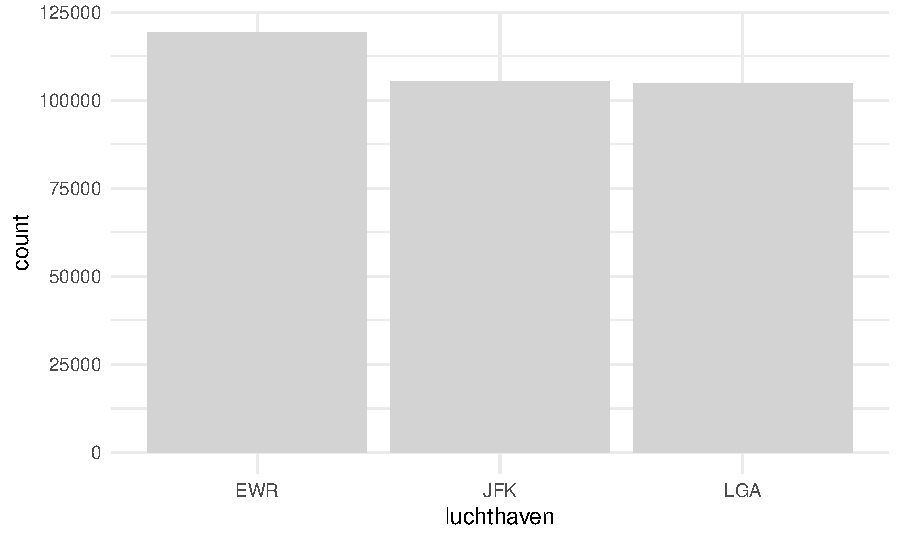
\includegraphics[width=1\linewidth]{textbook_files/figure-latex/2-3a-1} \caption[Staafdiagram luchthavens]{Staafdiagram luchthavens}\label{fig:2-3a}
\end{figure}

\begin{itemize}
\tightlist
\item
  Minder geschikt indien er veel waarden zijn. Dan wordt de X-as snel onleesbaar.(Fig. \ref{fig:2-3b})
\end{itemize}

\begin{figure}
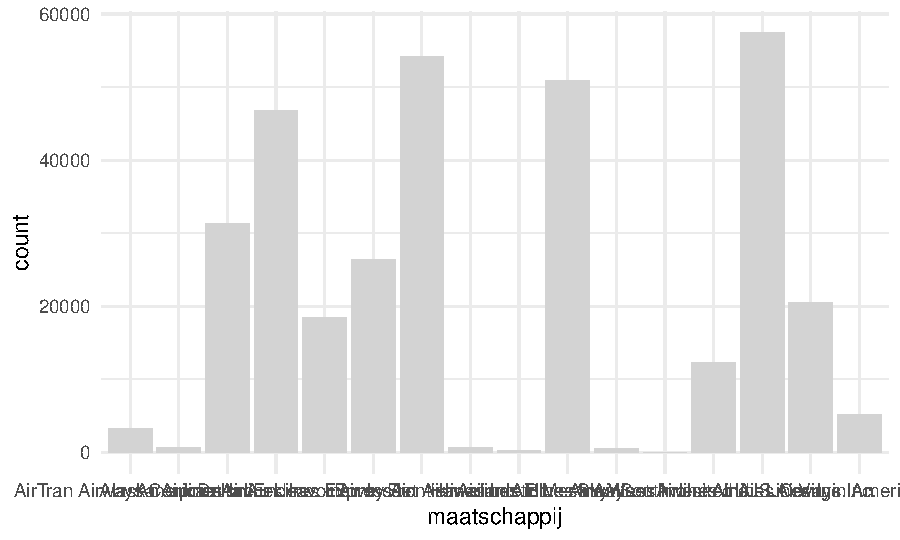
\includegraphics[width=1\linewidth]{textbook_files/figure-latex/2-3b-1} \caption[Staafdiagram maatschappijen]{Staafdiagram maatschappijen}\label{fig:2-3b}
\end{figure}

\begin{itemize}
\tightlist
\item
  Je kan natuurlijk de labels roteren. Maar dit kan nog steeds onhandig zijn om te lezen. (Fig. \ref{fig:2-3c}).
\end{itemize}

\begin{figure}
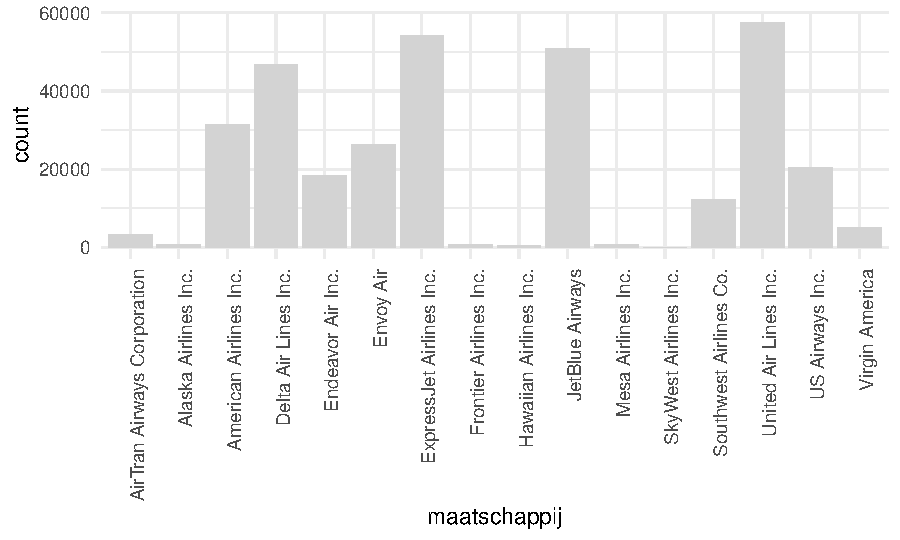
\includegraphics[width=1\linewidth]{textbook_files/figure-latex/2-3c-1} \caption[Staafdiagram met geroteerde labels]{Staafdiagram met geroteerde labels}\label{fig:2-3c}
\end{figure}

\begin{itemize}
\tightlist
\item
  In geval van een \textbf{nominale} variabele zijn er twee mogelijkheden om de waarden te rangschikken:

  \begin{itemize}
  \tightlist
  \item
    Alfabetisch. (standaard) Dit is handig om snel waarden terug te vinden.
  \item
    Volgens frequentie. Dit is handig om snel te zien welke waarden vaak/weinig voorkomen en geeft ook een beter beeld van de verdeling van de waarden. (Fig. \ref{fig:2-3d})
  \end{itemize}
\end{itemize}

\begin{figure}
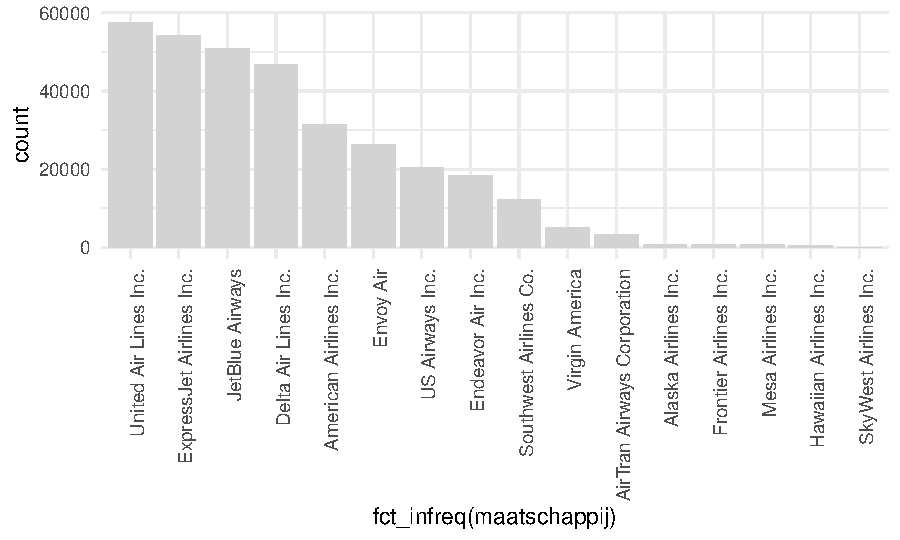
\includegraphics[width=1\linewidth]{textbook_files/figure-latex/2-3d-1} \caption[Staafdiagram gesorteerd op frequentie]{Staafdiagram gesorteerd op frequentie}\label{fig:2-3d}
\end{figure}

\begin{itemize}
\item
  In het geval van een \textbf{ordinale} variabele houd je best de intrinsieke volgorde van de waarden aan.
\item
  Je kan ook een horizontaal staafdiagram maken. (Fig. \ref{fig:2-3e})

  \begin{itemize}
  \tightlist
  \item
    Zelfde principe, maar dan met horizontale balken.
  \item
    Is handiger om de verschillende waarden te lezen, vooral indien dit er veel zijn.
  \end{itemize}
\end{itemize}

\begin{figure}
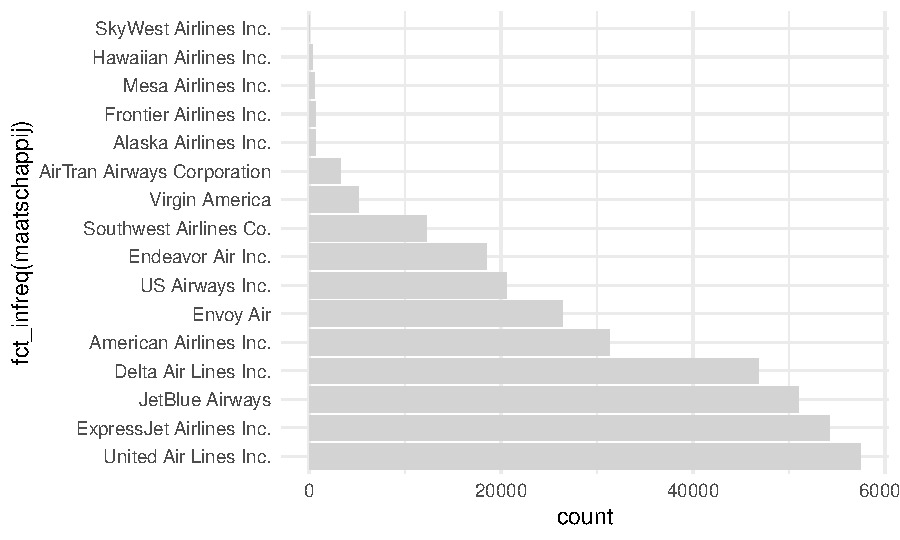
\includegraphics[width=1\linewidth]{textbook_files/figure-latex/2-3e-1} \caption[Verticaal staafdiagram gesorteerd op frequentie]{Verticaal staafdiagram gesorteerd op frequentie}\label{fig:2-3e}
\end{figure}

\hypertarget{dotplot}{%
\subsubsection{Dotplot}\label{dotplot}}

\begin{itemize}
\item
  In plaats van balken te gebruiken om de frequentie van een waarde aan te geven, kan je dit ook met punten doen. (Fig. \ref{fig:2-5a})
\item
  Een dotplot laat duidelijker zien waar de sprongen in de verdeling zit. Daarom is de dotplot vooral relevant als je de waarden ordent volgens frequentie.

  \begin{figure}
  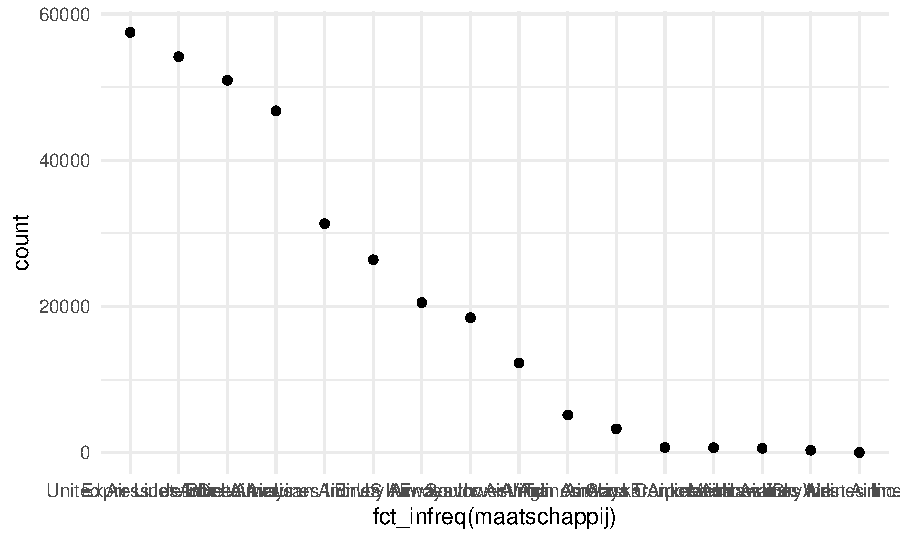
\includegraphics[width=1\linewidth]{textbook_files/figure-latex/2-5a-1} \caption[Dotplot maatschappij]{Dotplot maatschappij}\label{fig:2-5a}
  \end{figure}
\item
  Net als de barplot kan je zowel een verticale als horizontale dotplot maken. (Fig. \ref{fig:2-5b})
\end{itemize}

\begin{figure}
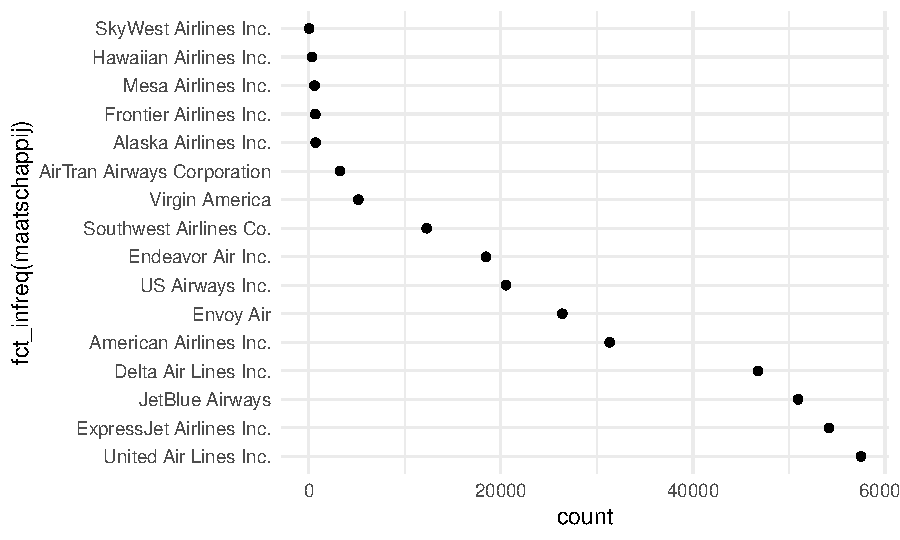
\includegraphics[width=1\linewidth]{textbook_files/figure-latex/2-5b-1} \caption[Verticale dotplot]{Verticale dotplot}\label{fig:2-5b}
\end{figure}

\hypertarget{stacked-staafdiagram}{%
\subsubsection{`Stacked' staafdiagram}\label{stacked-staafdiagram}}

\begin{itemize}
\tightlist
\item
  We maken nu slechts 1 kolom. Iedere waarde is een andere kleur en neemt een deel van de balk in beslag. De volledige balk stelt 100\% van de data voor. (Fig. \ref{fig:2-6a})
\item
  Kan nuttig zijn om data cumulatief te bestuderen.
\item
  Hiermee kunnen we vragen beantwoorden zoals: ``Welke waarden moeten we nemen om met zo weinig mogelijk waarden x\% van de objecten te hebben?''
\end{itemize}

\begin{figure}

{\centering 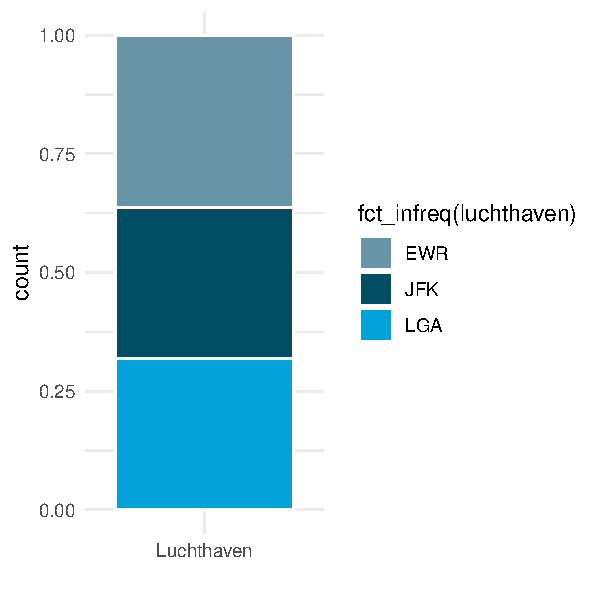
\includegraphics[width=0.7\linewidth]{textbook_files/figure-latex/2-6a-1} 

}

\caption[Stacked barplot]{Stacked barplot}\label{fig:2-6a}
\end{figure}

\begin{itemize}
\tightlist
\item
  We kunnen ook horizontale versies maken. (Fig. \ref{fig:2-6b})
\end{itemize}

\begin{figure}
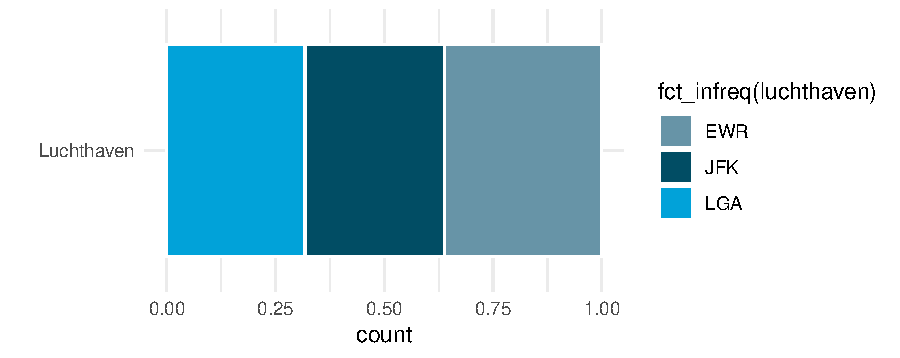
\includegraphics[width=1\linewidth]{textbook_files/figure-latex/2-6b-1} \caption[Horizontale stacked barplot]{Horizontale stacked barplot}\label{fig:2-6b}
\end{figure}

\begin{itemize}
\tightlist
\item
  Univariate stacked barcharts kunnen soms wat \emph{raar} overkomen. Vaak komt een gewone barchart beter over.
\end{itemize}

\hypertarget{andere-soorten}{%
\subsubsection{Andere soorten}\label{andere-soorten}}

\begin{itemize}
\tightlist
\item
  treemap: indelen van rechthoekige oppervlakte volgens categorische variabelen
\item
  pie chart

  \begin{itemize}
  \tightlist
  \item
    Moeilijk te interpreteren.
  \item
    Verschillen tussen waarden zijn enkel duidelijk bij grote verschillen, terwijl barplots en dotplots deze ook bij kleine verschillen kunnen tonen.
  \item
    Voor cumulatieve analyses van de data zijn barplots beter omdat het hier eenvoudiger is om af te leiden waar x\% zicht bevindt.
  \end{itemize}
\end{itemize}

\hypertarget{continue-variabele}{%
\subsection{Continue variabele}\label{continue-variabele}}

\hypertarget{histogram}{%
\subsubsection{Histogram}\label{histogram}}

\begin{itemize}
\tightlist
\item
  Analoog met barplot, alleen gaan we hier eerst onze ``categorieën'' definiëren. (Fig. \ref{fig:2-7a})
\item
  Dit wordt `binning' genoemd en wordt bepaald door een bin-breedte te kiezen.
\item
  Je kan de binbreedte rechtstreeks kiezen of bepalen door vast te leggen hoeveel categorieën/bins je wenst.
\end{itemize}

\begin{figure}
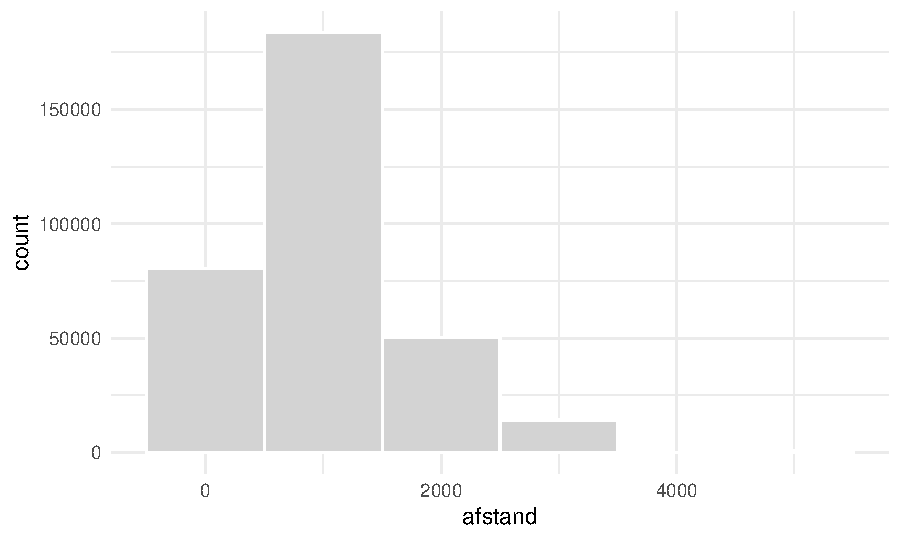
\includegraphics[width=1\linewidth]{textbook_files/figure-latex/2-7a-1} \caption[Histogram with binwidth 1000]{Histogram with binwidth 1000}\label{fig:2-7a}
\end{figure}

\begin{itemize}
\tightlist
\item
  Voor de visualisatie, worden alle waarden gegroepeerd per `bin'.
\item
  De binbreedte kan een enorme impact hebben op het uitzicht van de verdeling. (Fig. \ref{fig:2-7b} - \ref{fig:2-7c})

  \begin{itemize}
  \tightlist
  \item
    Hoe breder de bins, hoe minder modi je kan detecteren.
  \item
    Hoe smaller de bins, hoe meer modi je gaat zien, hoewel dit niet altijd even betekenisvol is.
  \item
    Hoe smaller de bins, hoe minder data er in iedere bin gaat zitten en dan kunnen patronen wel in jouw dataset bestaan maar louter ten gevolge van toeval.
  \end{itemize}
\end{itemize}

\begin{figure}
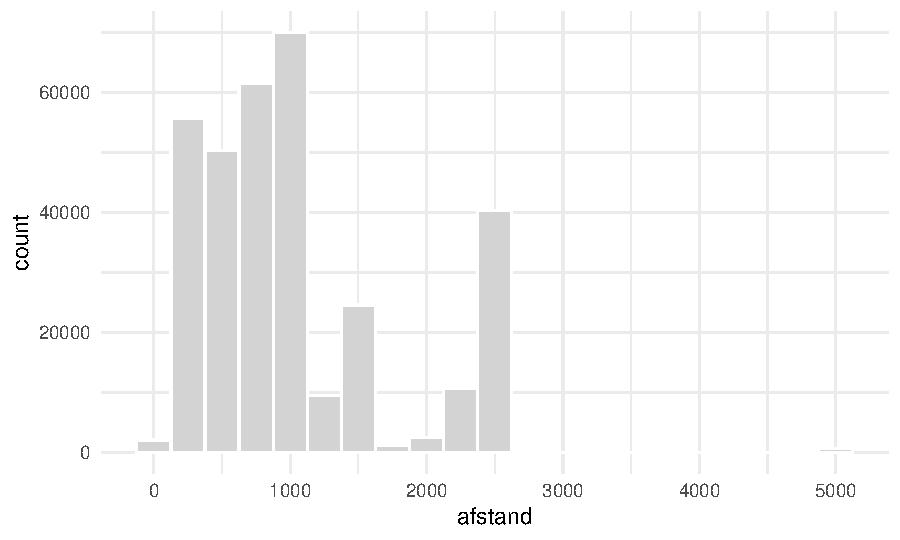
\includegraphics[width=1\linewidth]{textbook_files/figure-latex/2-7b-1} \caption[Histogram with binwidth 250]{Histogram with binwidth 250}\label{fig:2-7b}
\end{figure}

\begin{figure}
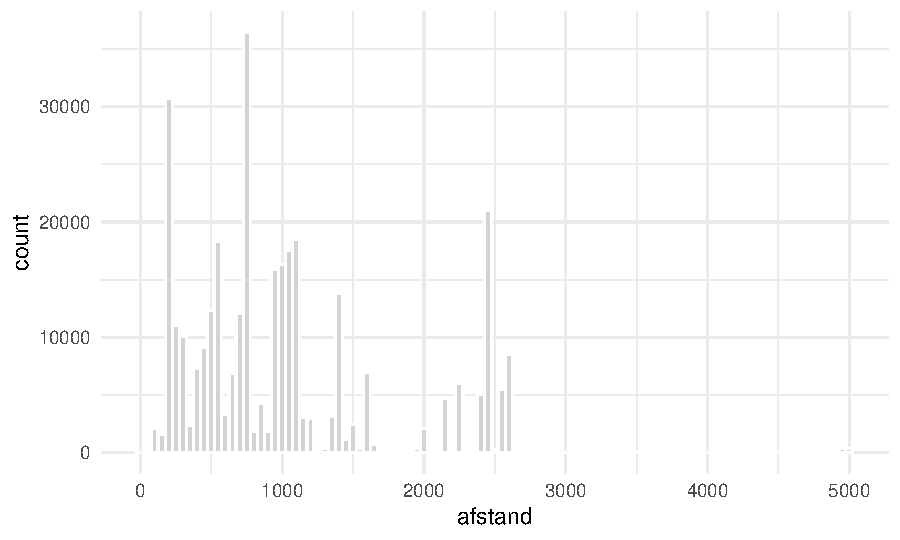
\includegraphics[width=1\linewidth]{textbook_files/figure-latex/2-7c-1} \caption[Histogram with binwidth 50]{Histogram with binwidth 50}\label{fig:2-7c}
\end{figure}

\hypertarget{density}{%
\subsubsection{Density}\label{density}}

\begin{itemize}
\tightlist
\item
  Variant van histogram.
\item
  In plaats van staven wordt er een curve getekend. (Fig. \ref{fig:2-density})
\item
  De oppervlakte onder de curve is steeds gelijk aan 1
\item
  Hoe hoger de curve, hoe meer observaties ter hoogt van deze waarde (hoe hoger de densiteit)
\item
  De waarde van de y-as heeft geen directe betekenis.
\end{itemize}

\begin{figure}
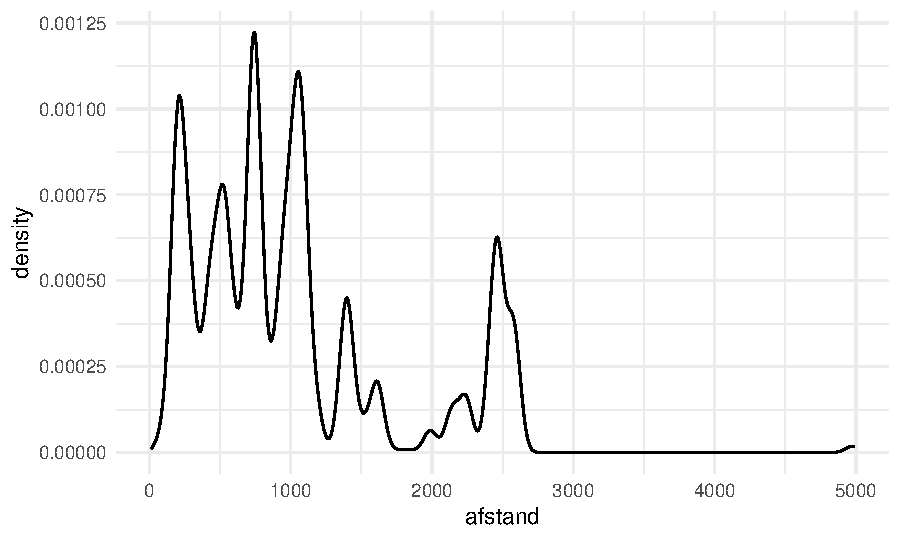
\includegraphics[width=1\linewidth]{textbook_files/figure-latex/2-density-1} \caption[Density plot]{Density plot}\label{fig:2-density}
\end{figure}

\hypertarget{boxplot}{%
\subsubsection{Boxplot}\label{boxplot}}

\begin{itemize}
\tightlist
\item
  De lijn in het midden duidt de mediaan aan. Dit betekent dat 50\% van je data onder deze lijn ligt, terwijl 50\% er boven ligt. (Fig. \ref{fig:2-8})
\item
  De box in het midden duidt de middelste 50\% van je data aan. Dit wordt ook de interkwartiel-box genoemd. Dit betekent dat 25\% van je data onder deze box zit en nog eens 25\% boven deze box ligt. Hoe groter de box, des te meer de data gespreid is.
\item
  Indien de box aan één zijde van de mediaanlijn groter is dan aan de andere zijde, dan wijst dit er op dat de data meer gespreid is aan die kant.
\item
  De ``whiskers'' geven de laatste datapunten aan die als ``normaal'' beschouwd worden. Datapunten buiten deze grenzen beschouwt een boxplot als outliers of extreme waarden.
\item
  De grens waar data van normaal naar extreem overgaat wordt door de boxplot bepaald door anderhalf keer de grootte van de interkwartiel-box op te tellen (en af te trekken) van de bovenste (onderste) grens van de interkwartiel-box. Punten die hier buiten liggen zijn outliers en worden als aparte punten aangeduid. De uitersten van de whiskers duiden de laatste datapunten aan binnen deze grenzen.
\end{itemize}

\begin{figure}

{\centering 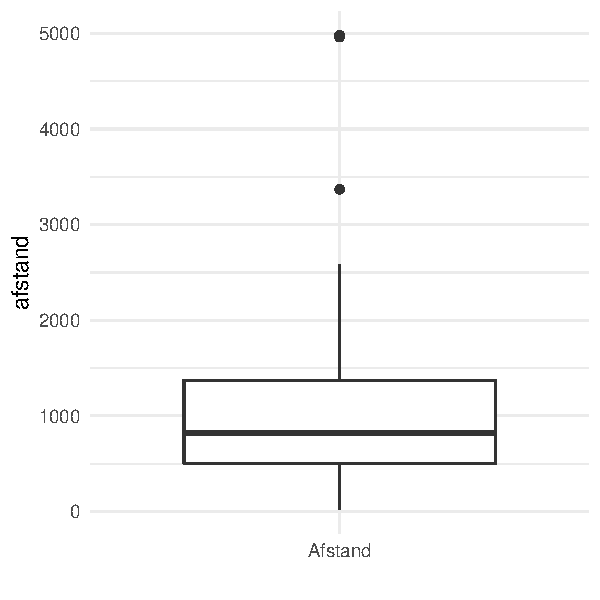
\includegraphics[width=0.7\linewidth]{textbook_files/figure-latex/2-8-1} 

}

\caption[Verticale boxplot vertrekvertraging]{Verticale boxplot vertrekvertraging}\label{fig:2-8}
\end{figure}

\begin{itemize}
\tightlist
\item
  Het is niet abnormaal dat er outliers in je data aanwezig zijn.
\item
  Bij normaal verdeelde data zal je gemiddeld 7 outliers per 1000 datapunten mogen verwachten.

  \begin{itemize}
  \tightlist
  \item
    Een normale verdeling is een bepaalde manier waarop data waarden verdeeld kunnen zijn die in de realiteit vaak voorkomt.
  \end{itemize}
\item
  Indien je echter veel meer outliers ziet op je boxplot visualisatie, dan is de kans reëel dat er meer aan de hand is:

  \begin{itemize}
  \tightlist
  \item
    Er zijn bijvoorbeeld systematische meetfouten
  \item
    De objecten in je data zijn in feite op bepaalde aspecten significant verschillend waardoor je ze apart zou moeten bestuderen.
  \end{itemize}
\item
  Je kan een boxplot ook roteren. (Fig \ref{fig:2-9})
\item
  Boxplots komen beter tot hun recht bij bivariate analyses dan bij univariate analyses.
\end{itemize}

\begin{figure}
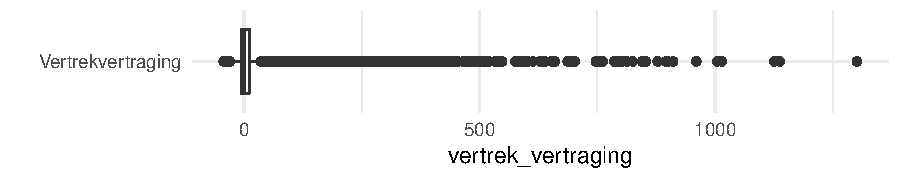
\includegraphics[width=1\linewidth]{textbook_files/figure-latex/2-9-1} \caption[Horizontale boxplot vertrekvertraging]{Horizontale boxplot vertrekvertraging}\label{fig:2-9}
\end{figure}

\hypertarget{violin-plot}{%
\subsubsection{Violin plot}\label{violin-plot}}

\begin{itemize}
\tightlist
\item
  Een violin plot kan je beschouwen als een combinatie van een histogram en een boxplot. (Fig. @ref(fig:2\_10a))
\item
  Net als bij een boxplot wordt op verticale wijze getoond hoe de data verspreid is.
\item
  Opnieuw kan je ervoor kiezen de grafiek te roteren. (Fig. @ref(fig:2\_10b))
\item
  Net als bij een histogram kan je goed zien waar het volume (de massa) van de data zich bevindt.
\item
  Net als bij een histogram kan je detecteren hoeveel modi de data bezit.
\item
  In tegenstelling tot de boxplot, kan je bij een violinplot wel niet duidelijk zien waar bijvoorbeeld het `midden' van je data is.
\end{itemize}

\begin{figure}

{\centering 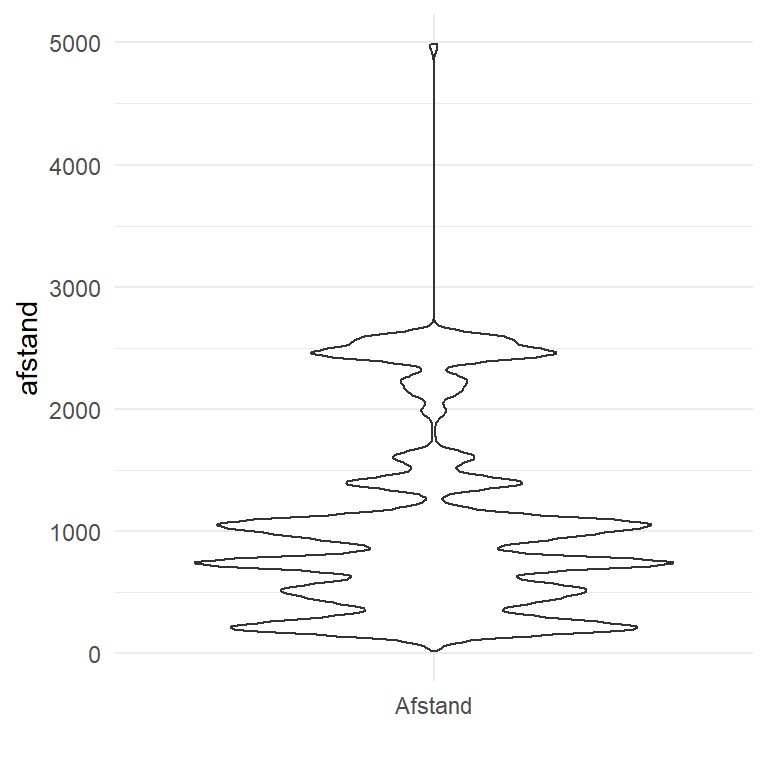
\includegraphics[width=0.7\linewidth]{textbook_files/figure-latex/2-10a-1} 

}

\caption[Verticale violin plot afstand]{Verticale violin plot afstand}\label{fig:2-10a}
\end{figure}

\begin{figure}
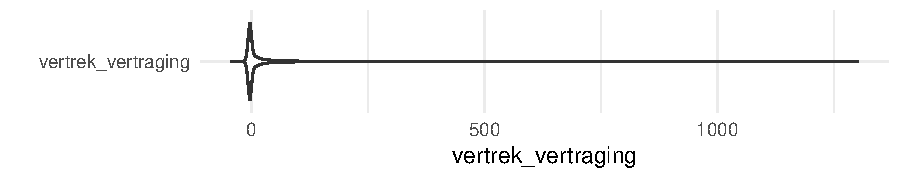
\includegraphics[width=1\linewidth]{textbook_files/figure-latex/2-10b-1} \caption[Horizontale violin plot vertrekvertraging]{Horizontale violin plot vertrekvertraging}\label{fig:2-10b}
\end{figure}

\hypertarget{jitter-plot}{%
\subsubsection{Jitter plot}\label{jitter-plot}}

\begin{itemize}
\tightlist
\item
  puntenwolk waarbij willekeurige ``noise'' (ruis) wordt toegevoegd.
\item
  de ruis zorgt ervoor dat datapunten niet overlappen, en dat het duidelijk is waar de massa zich bevindt.
\item
  Fig. \ref{fig:2-jitter} toont een vergelijking van violin, boxplot, point en jitter plot.
\end{itemize}

\begin{figure}
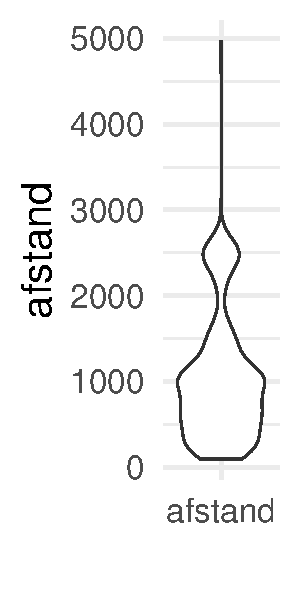
\includegraphics[width=0.24\linewidth]{textbook_files/figure-latex/2-jitter-1} 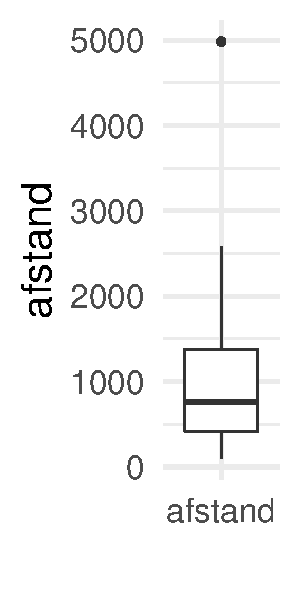
\includegraphics[width=0.24\linewidth]{textbook_files/figure-latex/2-jitter-2} 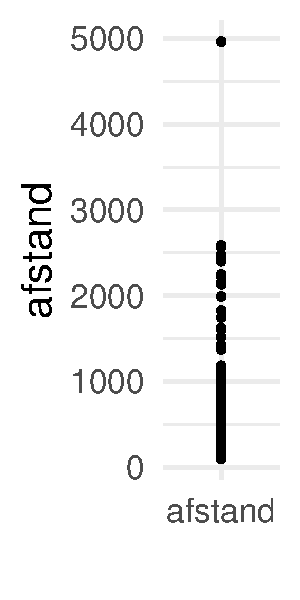
\includegraphics[width=0.24\linewidth]{textbook_files/figure-latex/2-jitter-3} 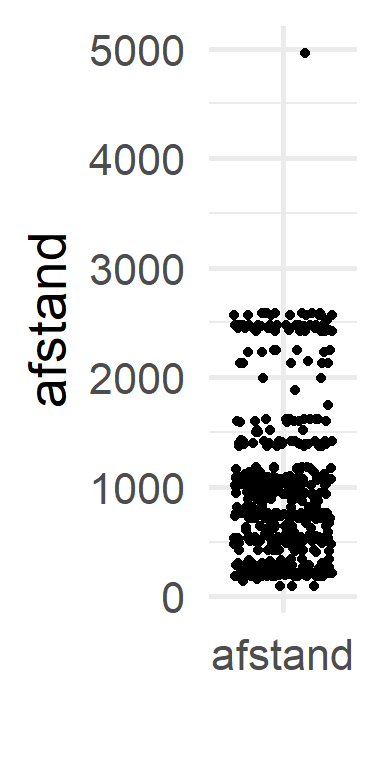
\includegraphics[width=0.24\linewidth]{textbook_files/figure-latex/2-jitter-4} \caption[Violin, boxplot, point en jitter]{Violin, boxplot, point en jitter}\label{fig:2-jitter}
\end{figure}

\hypertarget{bivariate-visualisatie-2-variabelen}{%
\section{Bivariate visualisatie (2 variabelen)}\label{bivariate-visualisatie-2-variabelen}}

\begin{itemize}
\tightlist
\item
  Wanneer we de relatie tussen 2 variabelen bekijken is het eenvoudig te denken in \emph{oorzaak} en gevolg \emph{termen.} \footnote{Zie opmerking i.v.m. correlatie versus causaliteit, \ref{how-charts-lie}.}

  \begin{itemize}
  \tightlist
  \item
    De variabele die we het label ``oorzaak'' geven, zullen we voortaan ``onafhankelijke variabele'' noemen.
  \item
    De variabele die we het label ``gevolg'' geven, zullen we voortaan ``afhankelijke variabele'' noemen.
  \end{itemize}
\item
  Waar we eigenlijk in geïnteresseerd zijn bij een visualisatie van 2 variabelen is de impact van de onafhankelijke variabele op de afhankelijke variabele weer te geven.
\item
  Alle vragen die we kunnen stellen bij de visualisatie van één variabele, kunnen we nog steeds stellen, met telkens de bijkomende vraag of het waargenomen patroon verandert als de onafhankelijke variabele van waarde verandert.
\end{itemize}

\hypertarget{situatie-1-de-onafhankelijke-variabele-is-categorisch}{%
\subsection{Situatie 1: De onafhankelijke variabele is categorisch}\label{situatie-1-de-onafhankelijke-variabele-is-categorisch}}

Indien de afhankelijke variabele een continue variabele is kan je:
* meerdere boxplots op 1 grafiek visualiseren, met telkens 1 boxplot per waarde van de onafhankelijke variabele. (Fig. \ref{fig:2-12a})

\begin{figure}
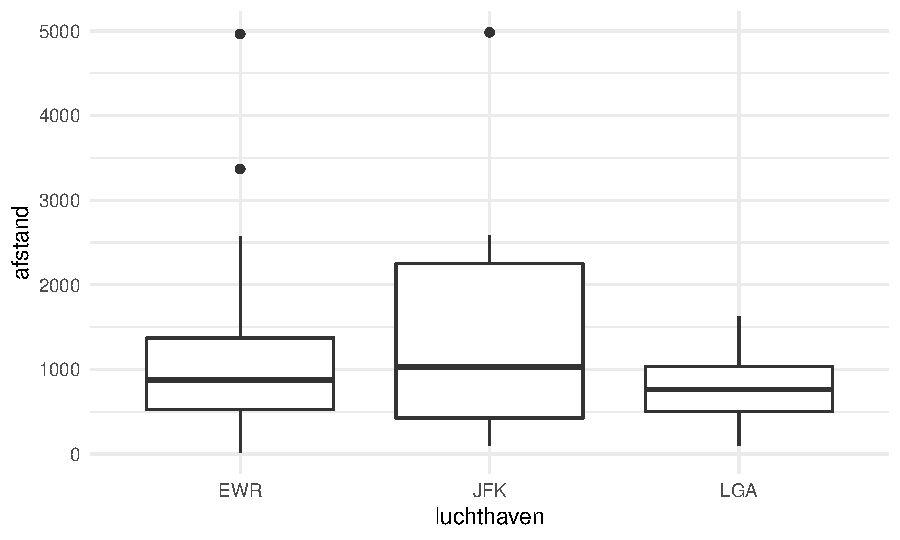
\includegraphics[width=1\linewidth]{textbook_files/figure-latex/2-12a-1} \caption[Bivariate boxplot]{Bivariate boxplot}\label{fig:2-12a}
\end{figure}

\begin{itemize}
\tightlist
\item
  meerdere violinplots op 1 grafiek tonen, met telkens 1 violinplot per waarde van de onafhankelijke variabele. (Fig. \ref{fig:2-12b})
\end{itemize}

\begin{figure}
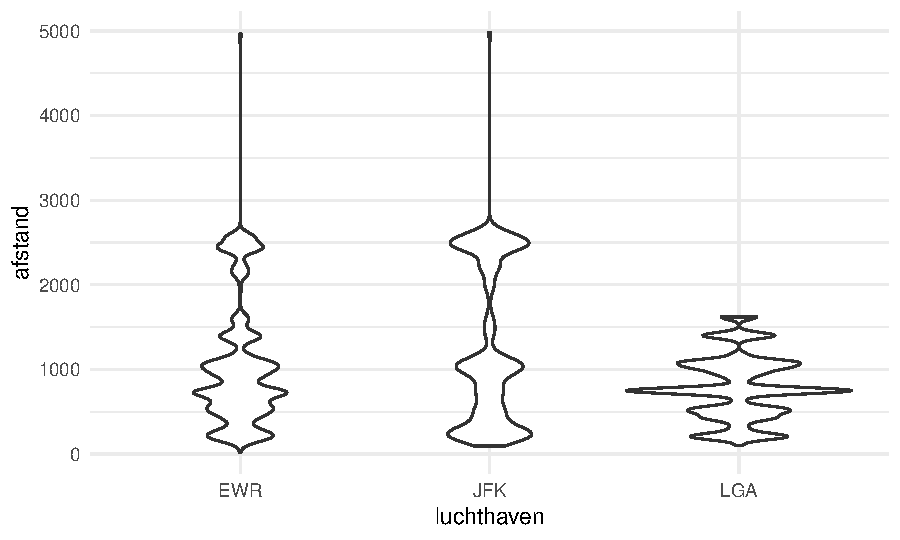
\includegraphics[width=1\linewidth]{textbook_files/figure-latex/2-12b-1} \caption[Bivariate violin plot]{Bivariate violin plot}\label{fig:2-12b}
\end{figure}

\begin{itemize}
\tightlist
\item
  meerdere histogrammen op 1 grafiek tonen

  \begin{itemize}
  \tightlist
  \item
    Hiervoor gebruiken we facetten: we tekenen voor elke waarde van de onafhankelijke variabele een apart assenstelsel. (Fig. \ref{fig:2-12c})
  \end{itemize}
\end{itemize}

\begin{figure}
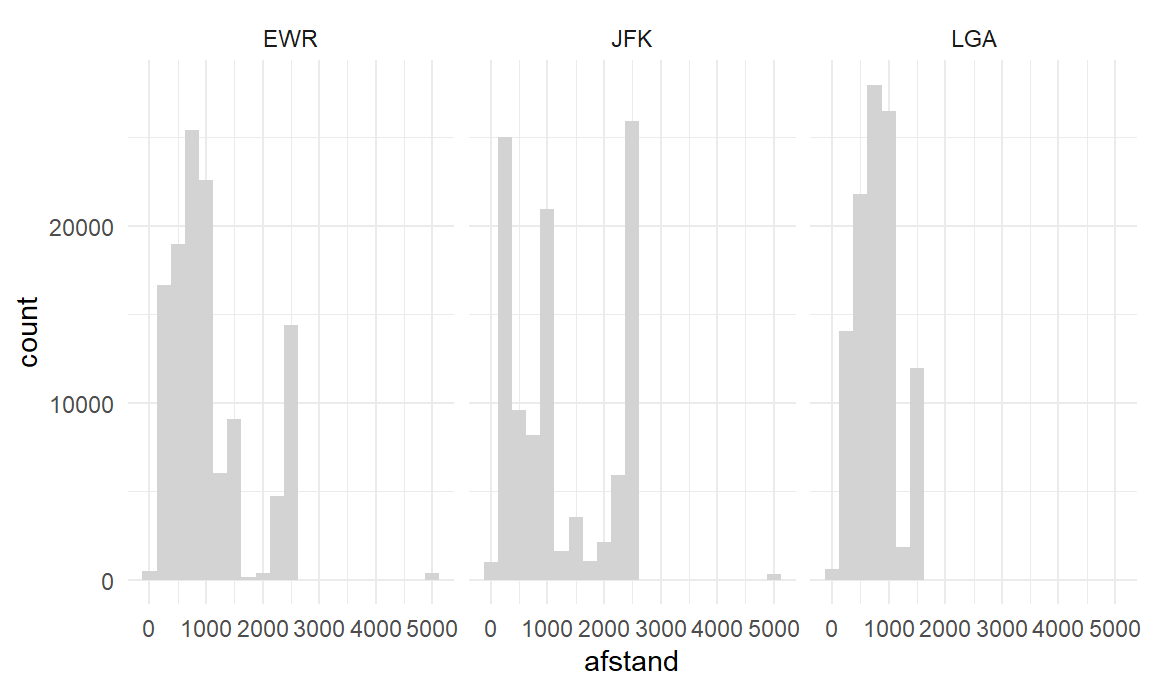
\includegraphics[width=1\linewidth]{textbook_files/figure-latex/2-12c-1} \caption[Bivariate histogram plot]{Bivariate histogram plot}\label{fig:2-12c}
\end{figure}

\begin{itemize}
\tightlist
\item
  meerdere density plots
\item
  Hiervoor kunnen we facetten gebruiken, ofwel de density plots over elkaar tekenen en onderscheiden met kleur. (Fig. \ref{fig:2-12d}-\ref{fig:2-12e})
\end{itemize}

\begin{figure}
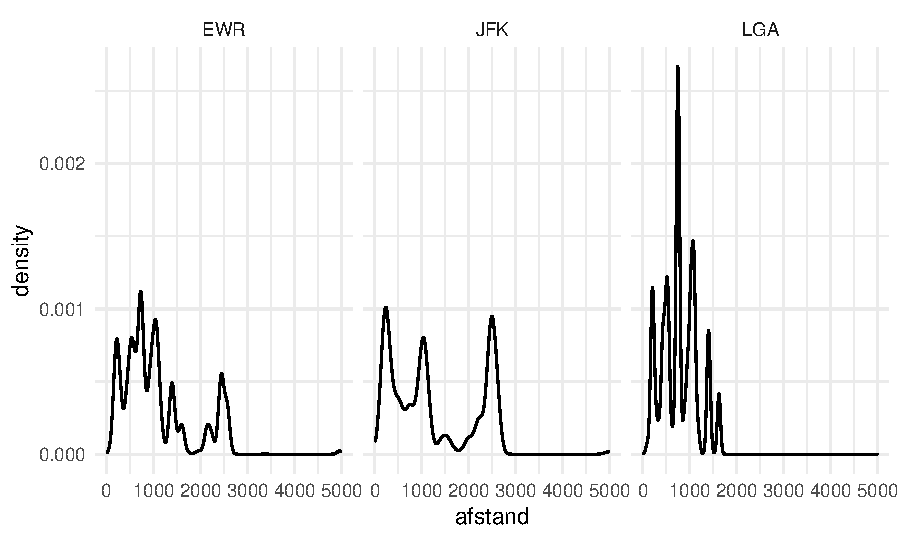
\includegraphics[width=1\linewidth]{textbook_files/figure-latex/2-12d-1} \caption[Bivariate density plot - apart]{Bivariate density plot - apart}\label{fig:2-12d}
\end{figure}

\begin{figure}
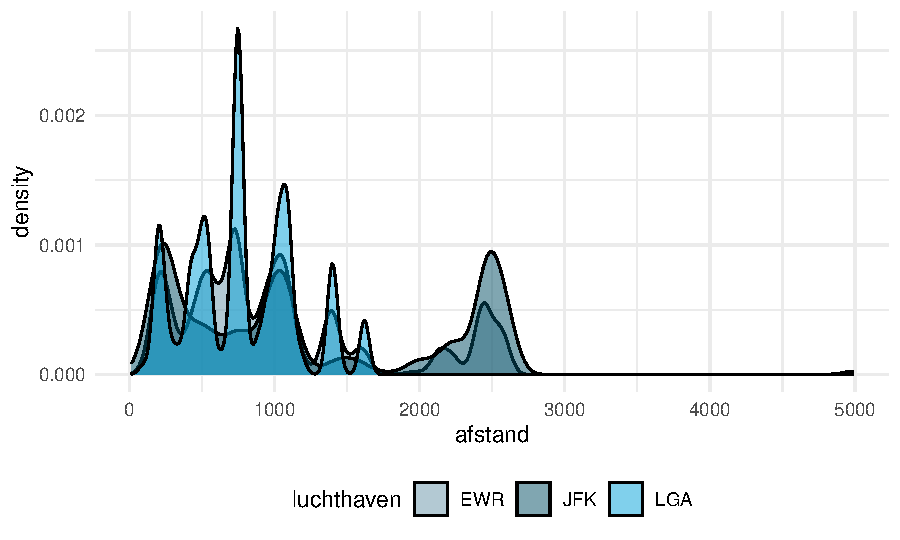
\includegraphics[width=1\linewidth]{textbook_files/figure-latex/2-12e-1} 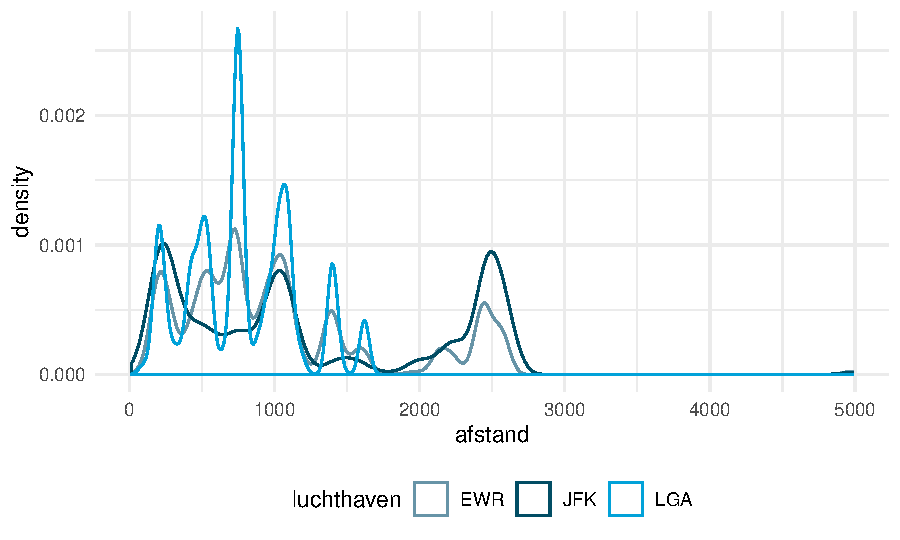
\includegraphics[width=1\linewidth]{textbook_files/figure-latex/2-12e-2} \caption[Bivariate density plot - overlappend]{Bivariate density plot - overlappend}\label{fig:2-12e}
\end{figure}

Indien de afhankelijke variabele een categorische variabele is:

\begin{itemize}
\tightlist
\item
  Kan je meerdere barplots op 1 grafiek visualiseren, met telkens de bars gegroepeerd per waarde van de onafhankelijke variabele.
\end{itemize}

\begin{figure}
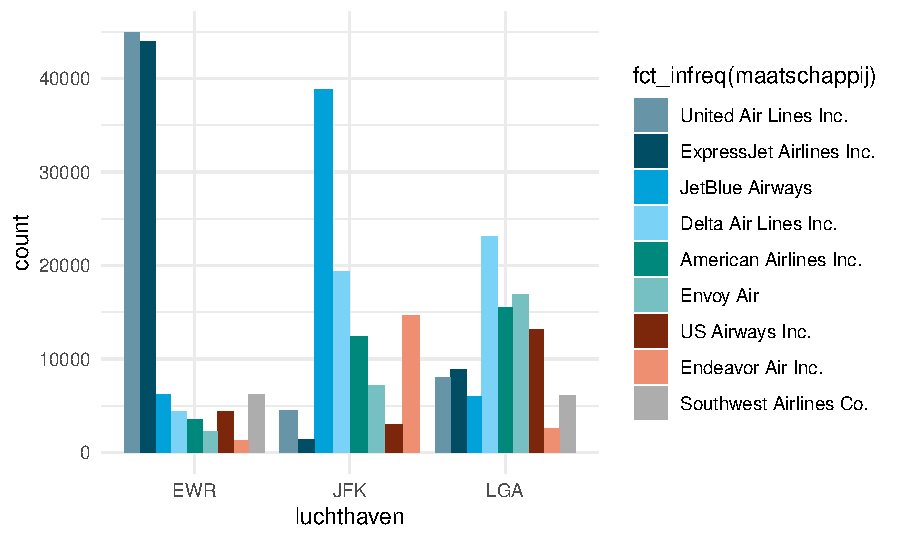
\includegraphics[width=1\linewidth]{textbook_files/figure-latex/2-13a-1} \caption[Bivariate barplot]{Bivariate barplot}\label{fig:2-13a}
\end{figure}

\begin{itemize}
\tightlist
\item
  Kan je meerdere stacked barplots op 1 grafiek plaatsen, met telkens een volledige stack per waarde van de onafhankelijke variabele.
\end{itemize}

\begin{figure}
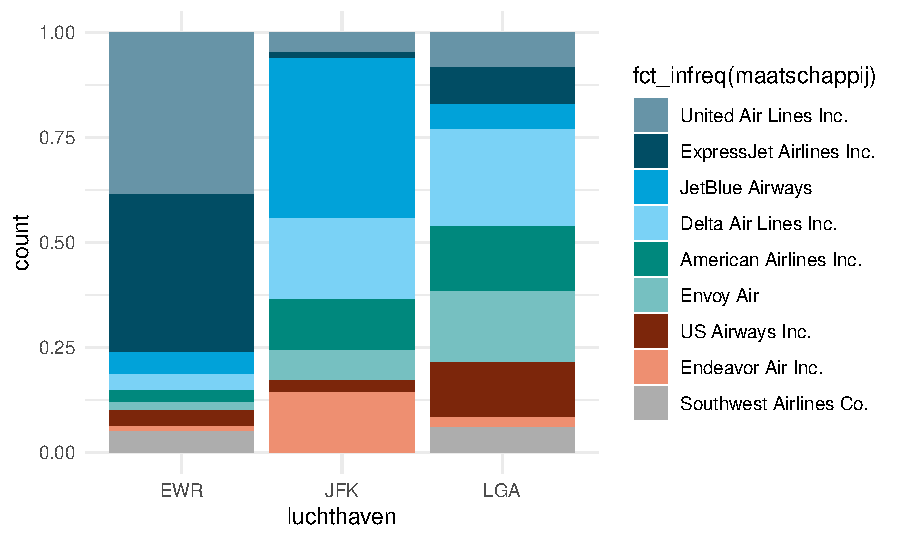
\includegraphics[width=1\linewidth]{textbook_files/figure-latex/2-13b-1} \caption[Bivariate stacked barplot]{Bivariate stacked barplot}\label{fig:2-13b}
\end{figure}

\begin{itemize}
\tightlist
\item
  Kan je een heatmap (of tile plot) gebruiken. Hier bij plaats je 2 categorische variabelen op de x-as en y-as, respectivelijk.

  \begin{itemize}
  \tightlist
  \item
    Voor elke combinatie van waarden is er een tegel die je kan inkleuren volgens de frequentie van de combinatie.
  \end{itemize}
\end{itemize}

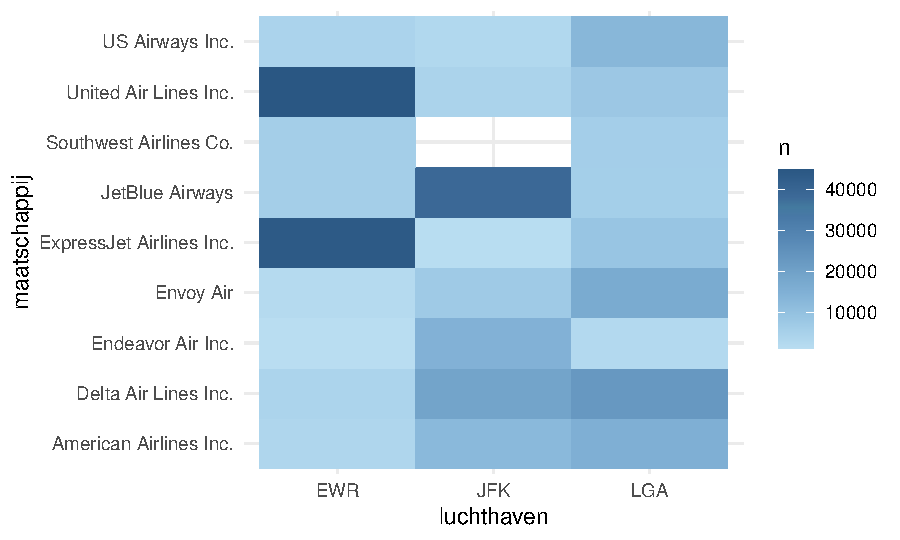
\includegraphics[width=1\linewidth]{textbook_files/figure-latex/unnamed-chunk-7-1}

\begin{itemize}
\tightlist
\item
  Je kan bijkomende ook de exacte waarde in elke tegel plotten.
\end{itemize}

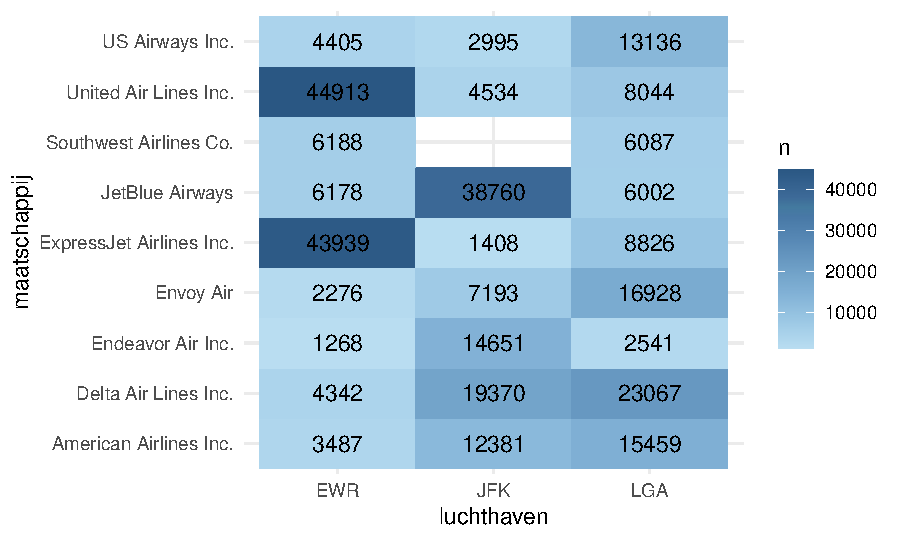
\includegraphics[width=1\linewidth]{textbook_files/figure-latex/unnamed-chunk-8-1}

\textbf{Let op} wanneer beide variabelen categorisch zijn, is het nog steeds van belang welke je beschouwd als afhankelijke en welke als onafhankelijke. Technisch kan je ze omdraaien, maar de betekenis van je visualizatie is niet dezelfde!

\begin{figure}
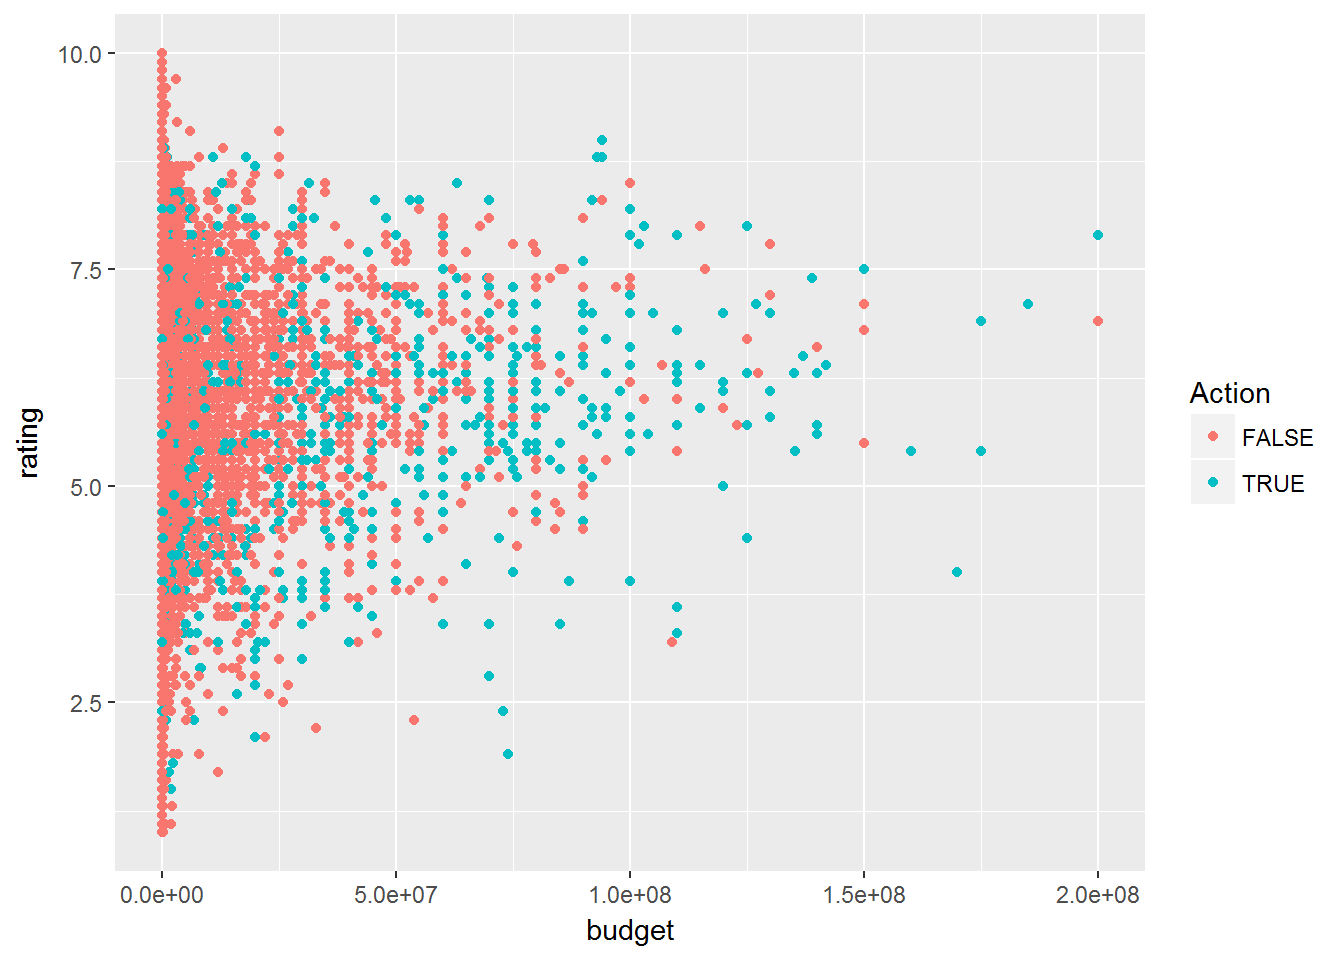
\includegraphics[width=1\linewidth]{textbook_files/figure-latex/unnamed-chunk-9-1} 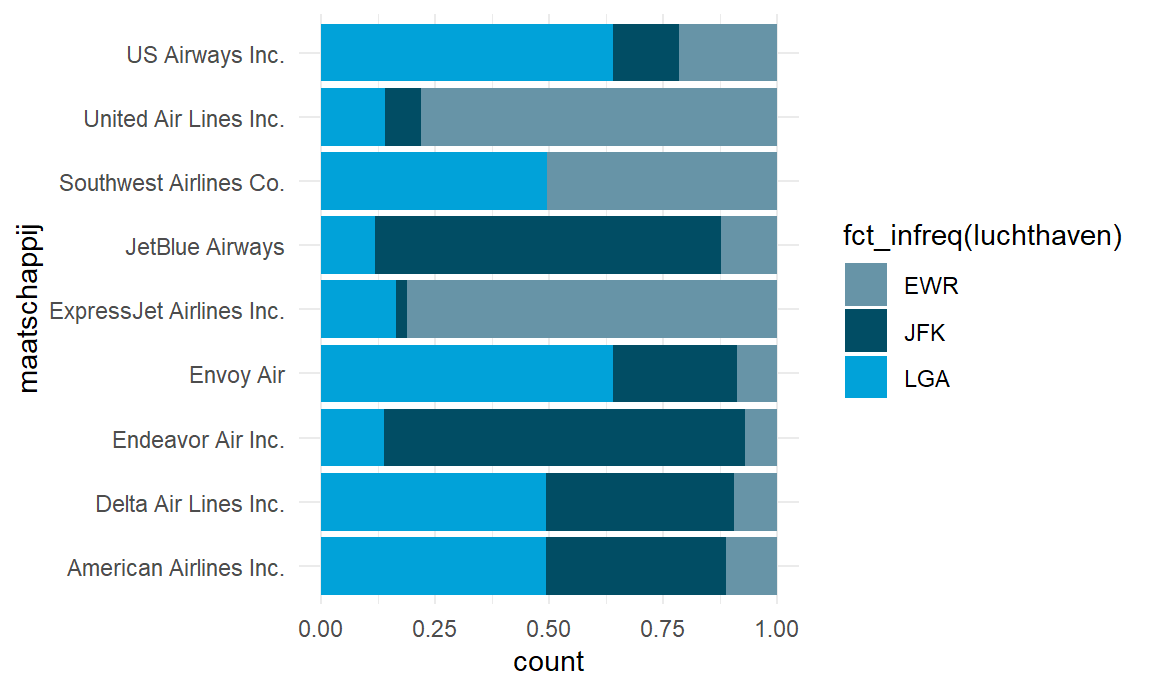
\includegraphics[width=1\linewidth]{textbook_files/figure-latex/unnamed-chunk-9-2} \caption[Twee verschillende stacked barcharts van luchthaven en maatschappij]{Twee verschillende stacked barcharts van luchthaven en maatschappij.}\label{fig:unnamed-chunk-9}
\end{figure}

Andere mogelijkheden:

\begin{itemize}
\tightlist
\item
  treemap
\end{itemize}

\begin{figure}
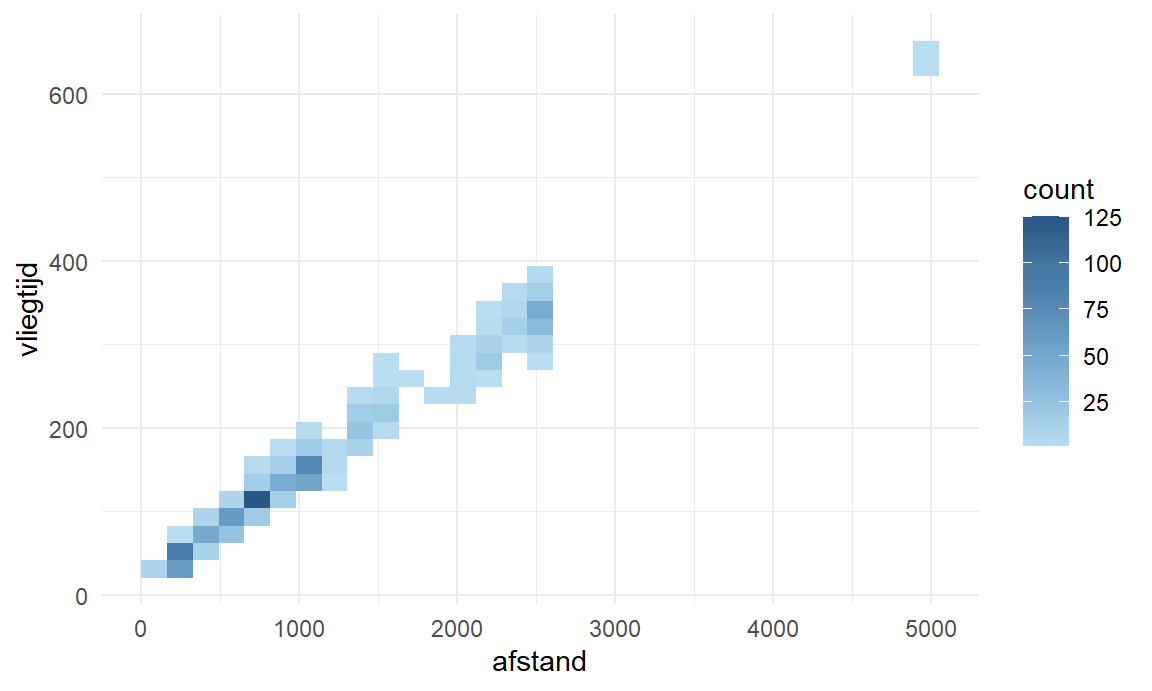
\includegraphics[width=1\linewidth]{textbook_files/figure-latex/unnamed-chunk-10-1} \caption[Treemap luchthaven en maatschappij]{Treemap luchthaven en maatschappij.}\label{fig:unnamed-chunk-10}
\end{figure}

\begin{itemize}
\tightlist
\item
  mosaic plot
\end{itemize}

\begin{figure}
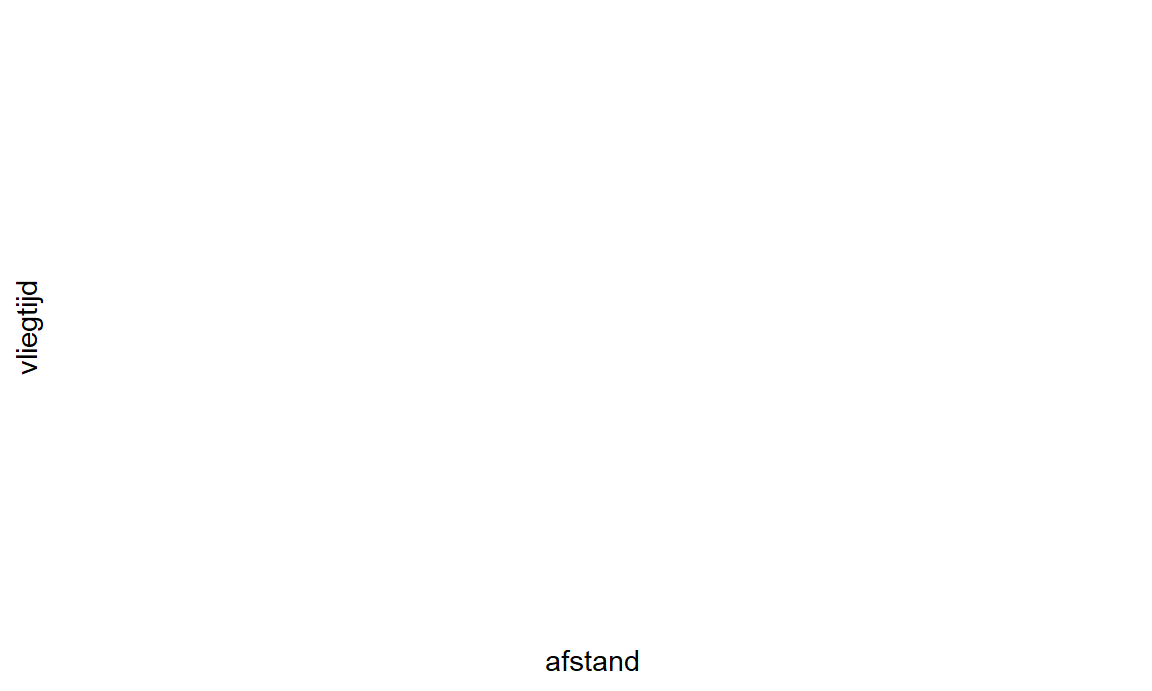
\includegraphics[width=1\linewidth]{textbook_files/figure-latex/unnamed-chunk-11-1} \caption[Mosaic plot luchthaven en maatschappij]{Mosaic plot luchthaven en maatschappij.}\label{fig:unnamed-chunk-11}
\end{figure}

\hypertarget{situatie-2-de-onafhankelijke-variabele-is-continue}{%
\subsection{Situatie 2: De onafhankelijke variabele is continue}\label{situatie-2-de-onafhankelijke-variabele-is-continue}}

\textbf{In dit geval kan je geen aparte plot per mogelijke waarde van de onafhankelijke variabele maken omdat er mogelijk oneindig veel waarden zijn.}

Indien de afhankelijke variabele continu is, dan kan je een scatterplot maken.

\begin{itemize}
\tightlist
\item
  Iedere observatie is een punt in je grafiek, waarbij de x-waarde op de grafiek overeenkomt met de waarde van de onafhankelijke variabele en de y-waarde op de grafiek overeenkomt met de waarde van de afhankelijke variabele.
\end{itemize}

\begin{figure}
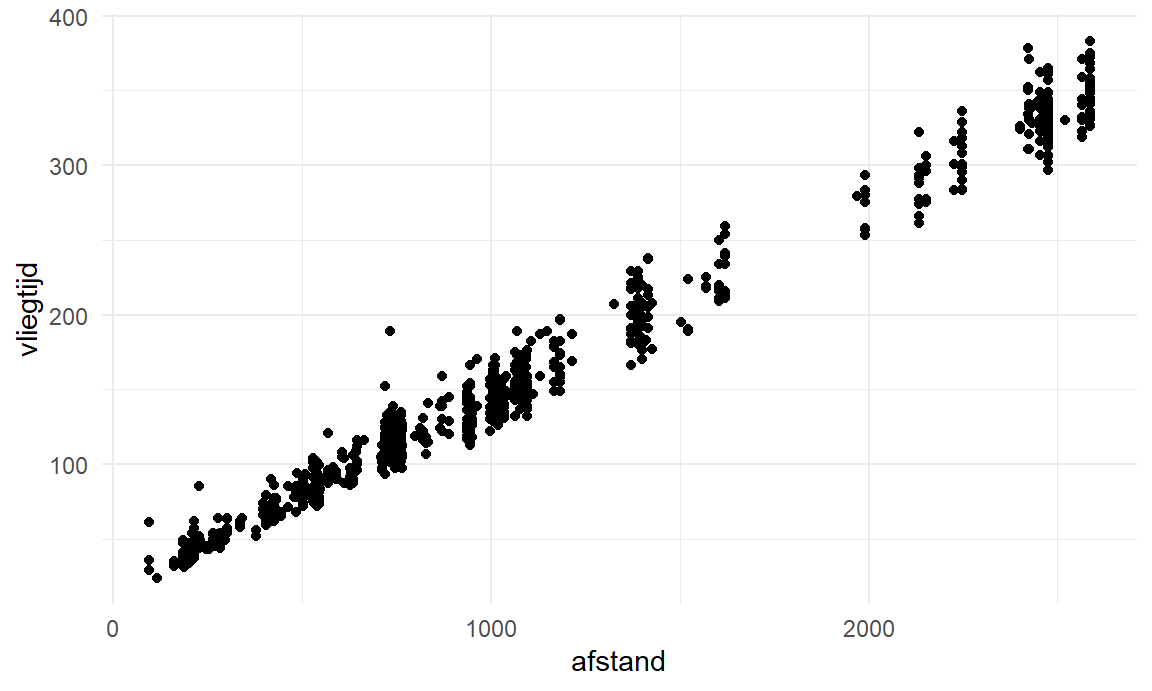
\includegraphics[width=1\linewidth]{textbook_files/figure-latex/213c-1} \caption[Scatterplot]{Scatterplot}\label{fig:213c}
\end{figure}

\begin{itemize}
\tightlist
\item
  Om patronen beter te herkennen kan je een ``trend-lijn'' toevoegen.
\end{itemize}

\begin{figure}
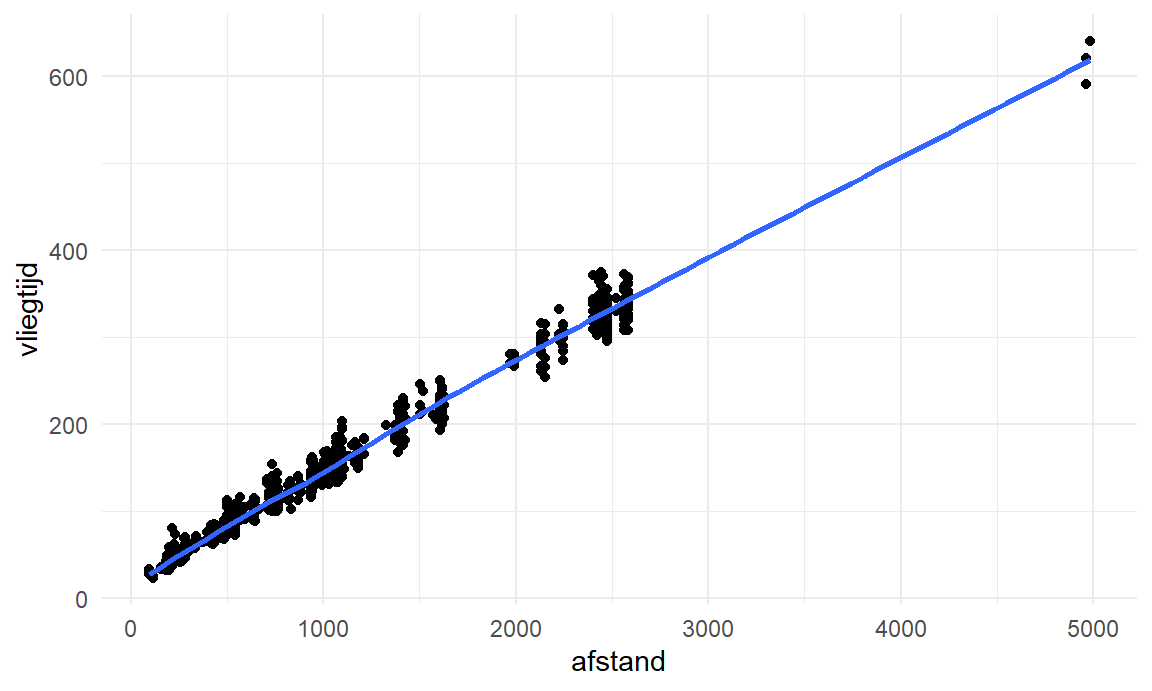
\includegraphics[width=1\linewidth]{textbook_files/figure-latex/2-13d-1} \caption[Scatterplot met trendlijn]{Scatterplot met trendlijn}\label{fig:2-13d}
\end{figure}

\begin{itemize}
\tightlist
\item
  Bij scatterplots is er gevaar voor overplotting
\item
  Mogelijke oplossingen

  \begin{itemize}
  \tightlist
  \item
    2D histogram: verdeel veld op in vierkante bins en tel per bin hoeveel data punten er zijn
  \item
    Hexplot: analoog, maar gebruik zeshoekige bins ipv vierkanten. Voordeel: punten binnen elke zeshoek liggen dichter bij het middelpunt van de bin.
  \end{itemize}
\end{itemize}

\begin{figure}
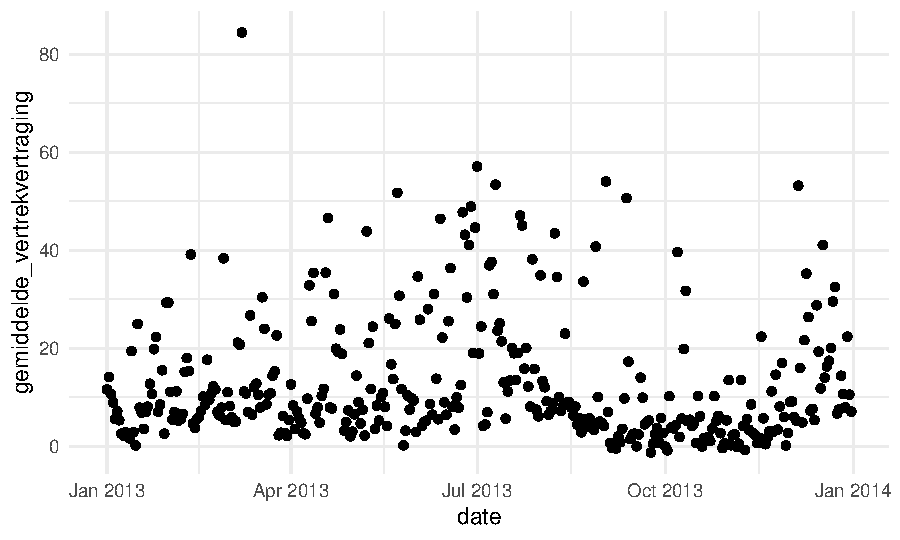
\includegraphics[width=1\linewidth]{textbook_files/figure-latex/unnamed-chunk-12-1} \caption[Scatterplot met trendlijn]{Scatterplot met trendlijn}\label{fig:unnamed-chunk-12}
\end{figure}

\begin{figure}
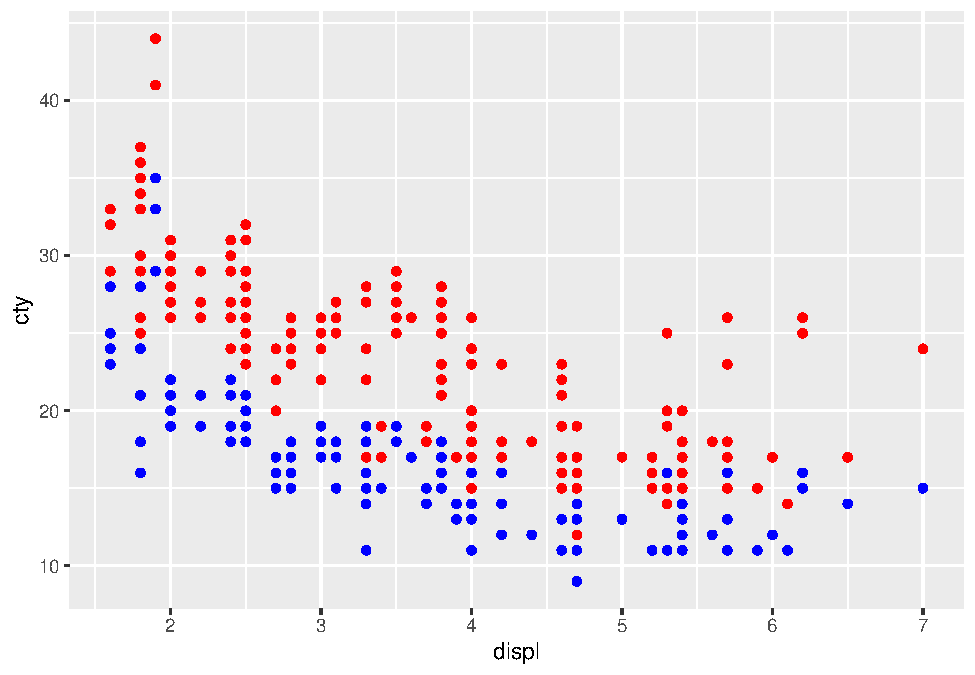
\includegraphics[width=1\linewidth]{textbook_files/figure-latex/unnamed-chunk-13-1} \caption[Hexplot met trendlijn]{Hexplot met trendlijn}\label{fig:unnamed-chunk-13}
\end{figure}

Indien de afhankelijke variabele categorisch is, dan kan je niet rechtstreeks een betekenisvolle plot maken omdat er waarschijnlijk te weinig datapunten zijn voor iedere mogelijke waarde van de onafhankelijke variabele.

\begin{itemize}
\tightlist
\item
  Wat je dan best kan doen, is de onafhankelijke continue variabele categorisch maken door deze in te delen in bins/intervallen. En dan ben je terug in de situatie waarbij de onafhankelijke variabele categorisch is. We komen hierop terug in het hoofdstuk over Data Voorbereiding.
\end{itemize}

\hypertarget{situatie-3-de-onafhankelijke-variabele-is-tijd}{%
\subsection{Situatie 3: De onafhankelijke variabele is tijd}\label{situatie-3-de-onafhankelijke-variabele-is-tijd}}

\begin{itemize}
\tightlist
\item
  Tijd kunnen we zien als continue variabele

  \begin{itemize}
  \tightlist
  \item
    Bijgevolg zelfde grafieken mogelijk als wanneer onafhankelijke variabele continue is

    \begin{itemize}
    \tightlist
    \item
      Tijd + continue afhankelijk -\textgreater{} scatterplot, 2D histograms, hex bins
    \item
      Tijd + categorisch afhankelijk -\textgreater{} probleem: tijd categoriseren (zie verder).
    \end{itemize}
  \end{itemize}
\item
  Wanneer we één enkele variabele voorstellen doorheen de tijd is er per tijdseenheid maar 1 data punt. Hieronder wordt de gemiddelde vertrekvertraging per dag getoond.\\

  \begin{figure}
  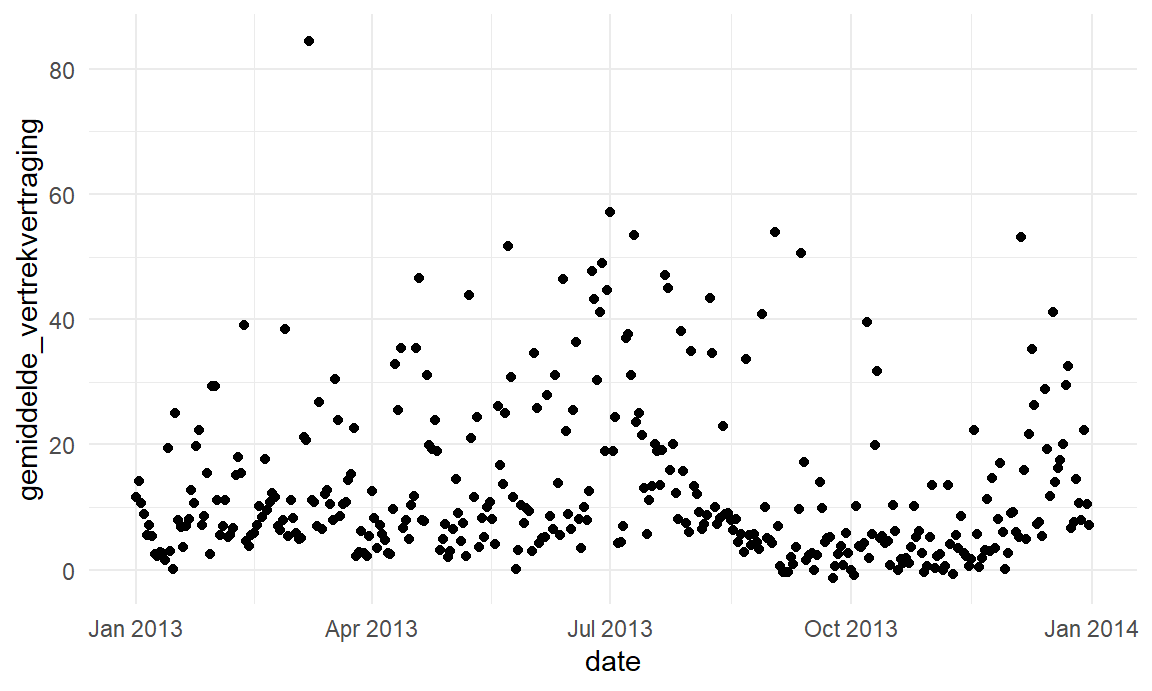
\includegraphics[width=1\linewidth]{textbook_files/figure-latex/unnamed-chunk-14-1} \caption[Puntenwolk met tijd op x-as]{Puntenwolk met tijd op x-as}\label{fig:unnamed-chunk-14}
  \end{figure}
\end{itemize}

In dat geval is het beter om in plaats van punten een lijngrafiek te gebruiken.

\begin{figure}
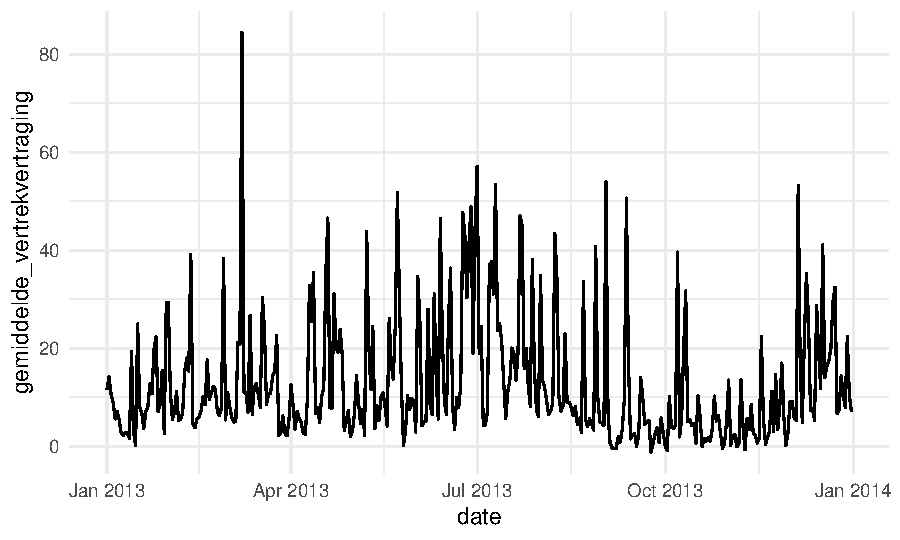
\includegraphics[width=1\linewidth]{textbook_files/figure-latex/unnamed-chunk-15-1} \caption[Lijngrafiek]{Lijngrafiek}\label{fig:unnamed-chunk-15}
\end{figure}

Indien je een beperkt aantal punten hebt (hieronder bijvoorbeeld één maand van de vluchtgegevens) kan je ervoor kiezen om zowel punten als lijnen te tonen. Op die manier is het makkelijker individuele data punten af te lezen.

\begin{figure}
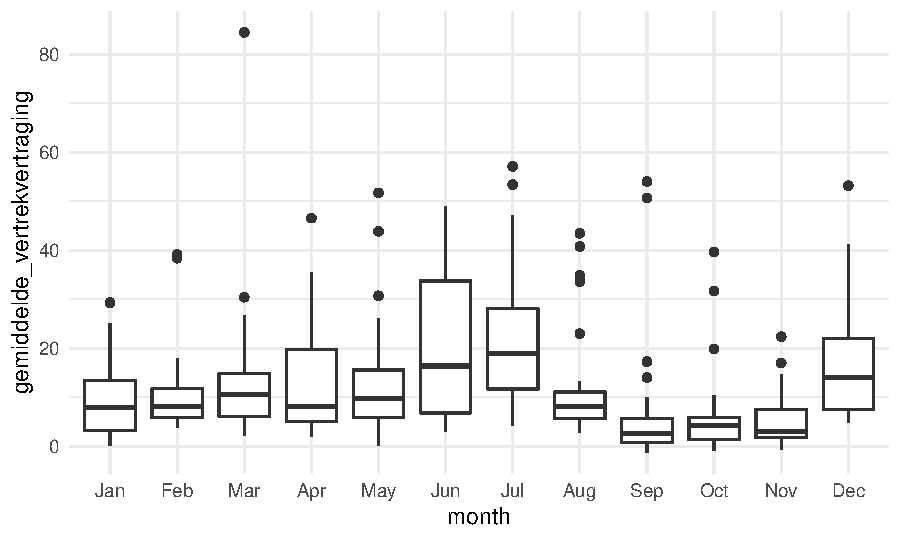
\includegraphics[width=1\linewidth]{textbook_files/figure-latex/unnamed-chunk-16-1} \caption[Lijn grafiek met punten]{Lijn grafiek met punten}\label{fig:unnamed-chunk-16}
\end{figure}

Indien we veel datapunten hebben, wat hier het geval is, kan een lijngrafiek zeer chaotisch worden. We kunnen daarom ervoor kiezen om onze tijd in te delen in categoriëen. Bijvoorbeeld, in plaats van de dagelijkse gemiddelde vertrekvertraging, kunnen we de gemiddelde vertrekvertraging per maand berekenen en tonen.

\begin{figure}
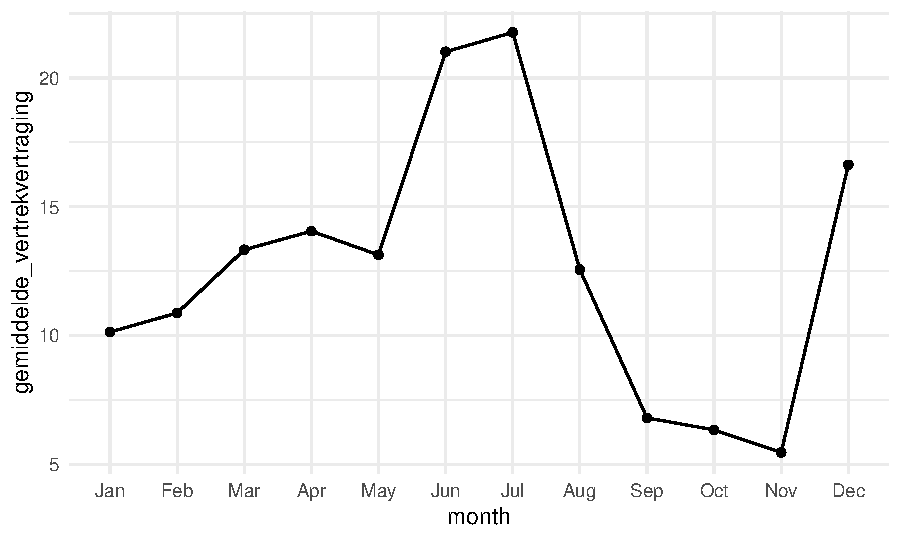
\includegraphics[width=1\linewidth]{textbook_files/figure-latex/unnamed-chunk-17-1} \caption[Lijngrafiek van gemiddelde vertrekvertraging per maand]{Lijngrafiek van gemiddelde vertrekvertraging per maand.}\label{fig:unnamed-chunk-17}
\end{figure}

\begin{itemize}
\tightlist
\item
  Op dit moment verliezen we daardoor wel veel informatie. Maar we kunnen dit nu ook beschouwen als een visualizatie van een categorische variabele (maand) t.o.v. een continue. Waardoor we de technieken voor dit type bivariate visualizaties kunnen toepassen. Bijvoorbeeld boxplots. We zien nu zowel de algemene trend als outliers. In februari was er bijvoorbeeld een dag waar de gemiddelde vertraging ver boven de normale trend lag.
\end{itemize}

\begin{figure}
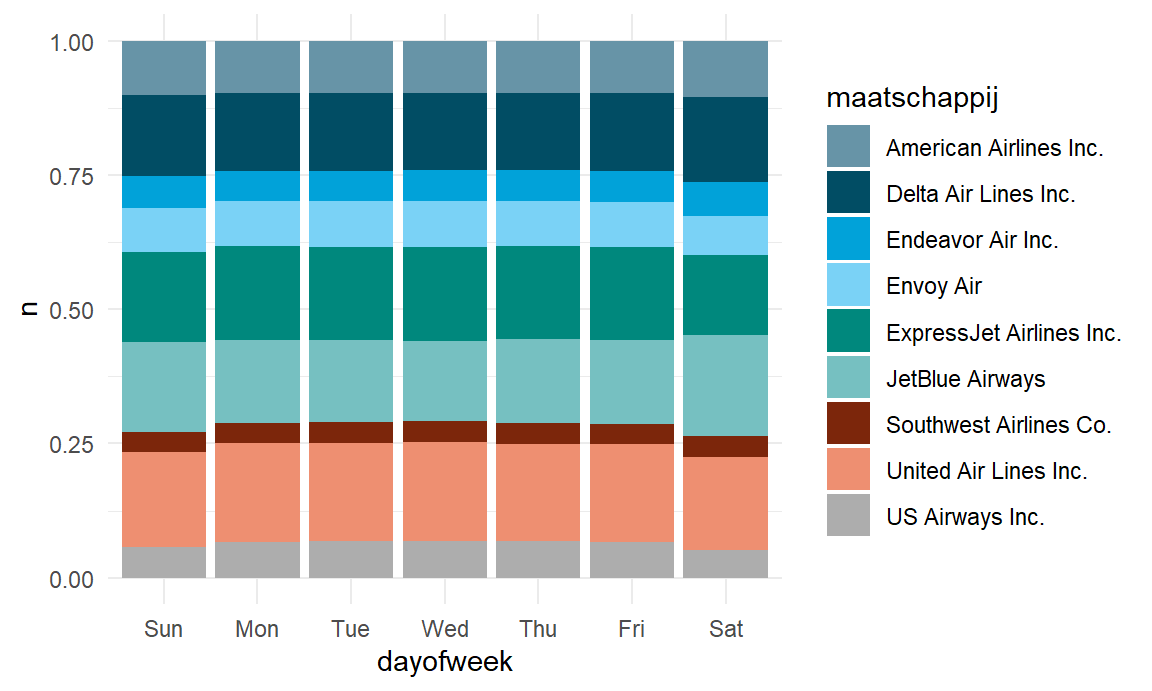
\includegraphics[width=1\linewidth]{textbook_files/figure-latex/unnamed-chunk-18-1} \caption[Boxplots van gemiddelde dagelijske vertrekvertraging voor elke maand]{Boxplots van gemiddelde dagelijske vertrekvertraging voor elke maand.}\label{fig:unnamed-chunk-18}
\end{figure}

\begin{itemize}
\tightlist
\item
  Wanneer we de tijd gecategoriseerd hebben kunnen we ook categorische variabelen weergeven als afhankelijke. Bijvoorbeeld, zijn er verschillen in het aantal vluchten per maatschappij doorheen de tijd. We kunnen hier dezelfde types grafieken als voor bivariate cat+cat visualizaties gebruiken, bijvoorbeeld stacked barcharts.
\end{itemize}

\begin{figure}
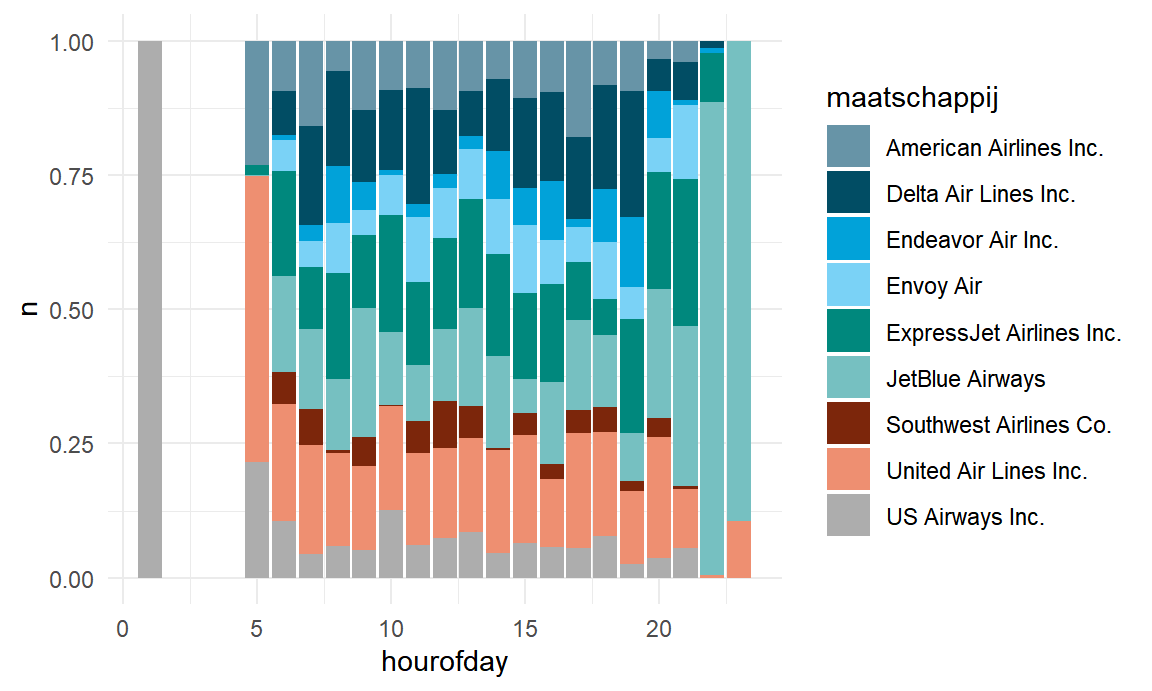
\includegraphics[width=1\linewidth]{textbook_files/figure-latex/unnamed-chunk-19-1} \caption[Verdeling van aantal vluchten over maatschappijen per maand]{Verdeling van aantal vluchten over maatschappijen per maand.}\label{fig:unnamed-chunk-19}
\end{figure}

\begin{itemize}
\tightlist
\item
  We kunnen categorizeren op maand, jaar, etc. Maar ook op tijdspecifiekere kenmerken, zoals bijvoorbeeld de dag van de week
\end{itemize}

\begin{figure}
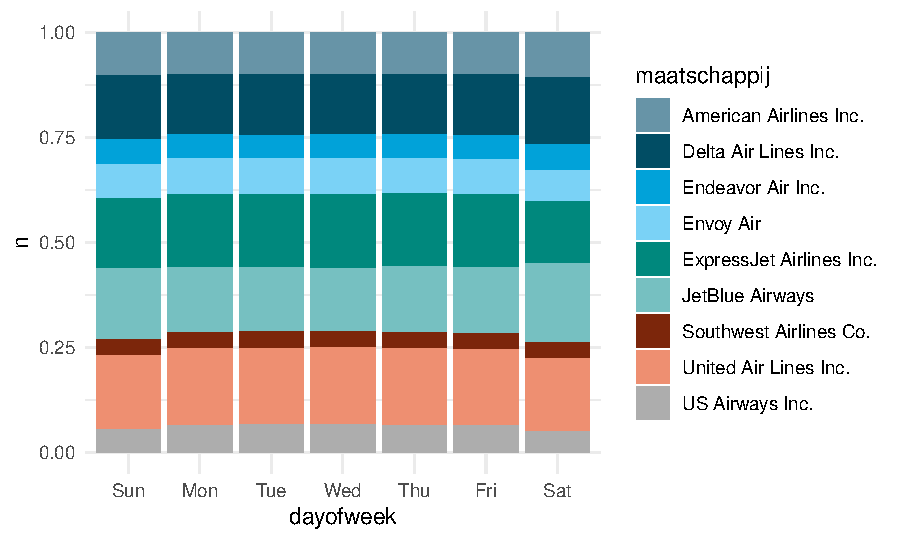
\includegraphics[width=1\linewidth]{textbook_files/figure-latex/unnamed-chunk-20-1} \caption[Verdeling van aantal vluchten over maatschappijen per dag van de week]{Verdeling van aantal vluchten over maatschappijen per dag van de week.}\label{fig:unnamed-chunk-20}
\end{figure}

\begin{itemize}
\tightlist
\item
  Of het uur van de dag
\end{itemize}

\begin{figure}
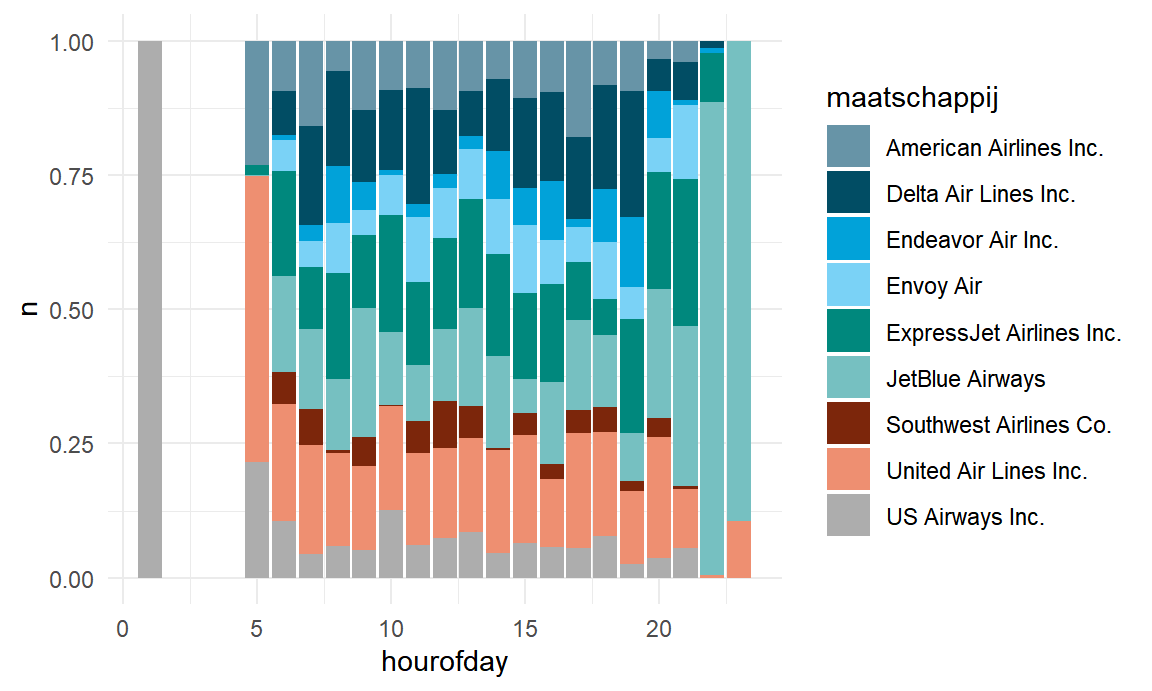
\includegraphics[width=1\linewidth]{textbook_files/figure-latex/unnamed-chunk-21-1} \caption[Verdeling van aantal vluchten over maatschappijen per vertrekuur]{Verdeling van aantal vluchten over maatschappijen per vertrekuur.}\label{fig:unnamed-chunk-21}
\end{figure}

\hypertarget{multivariate-visualisaties-meer-dan-2-variabelen}{%
\section{Multivariate visualisaties (meer dan 2 variabelen)}\label{multivariate-visualisaties-meer-dan-2-variabelen}}

\begin{itemize}
\tightlist
\item
  Datavisualisatie van patronen tussen meer dan 2 variabelen worden snel te complex om te interpreteren.
\item
  Het basisprincipe is wel eenvoudig.

  \begin{itemize}
  \tightlist
  \item
    Je hebt typisch 1 afhankelijke variabele (Y) en een aantal onafhankelijke variabelen (A, B, \ldots).
  \item
    Je visualizeert eerst Y en A (bivariaat)
  \item
    Je voegt dan de volgende variabelen (B, c, \ldots) stap voor stap toe aan de grafiek.

    \begin{itemize}
    \tightlist
    \item
      Door de bivariate grafiek te herhalen in verschillende facetten (een voor elke waarde van B).
    \item
      Door verschillende kleuren te gebruiken voor elke waarde van B
    \end{itemize}
  \end{itemize}
\item
  Bij multivariate visualisaties zijn er afhankelijk van de data types oneidig veel mogelijke grafieken die je kan maken.

  \begin{itemize}
  \tightlist
  \item
    Het is vaak afhankelijk van de data welke grafiek het ``best past''
  \item
    Enkel wanneer de onafhankelijk variabele continu is zijn de keuzes beperkt en ben je vaak genoodzaakt om deze om te zetten naar categoriëen.
  \end{itemize}
\end{itemize}

\hypertarget{voorbeeld-in-welke-mate-hangt-de-vertrek-vertraging-af-van-de-luchthaven-en-de-afstand}{%
\subsection{Voorbeeld: In welke mate hangt de vertrek vertraging af van de luchthaven en de afstand?}\label{voorbeeld-in-welke-mate-hangt-de-vertrek-vertraging-af-van-de-luchthaven-en-de-afstand}}

Stap 1. Vertraging vs.~afstand

\begin{itemize}
\tightlist
\item
  Beide continue: scatterplot
\end{itemize}

\begin{figure}
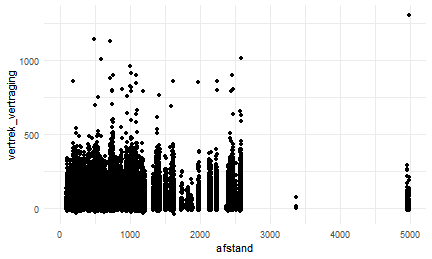
\includegraphics[width=1\linewidth]{textbook_files/figure-latex/labelke-1} \caption[Vertrekvertraging vs afstand]{Vertrekvertraging vs afstand}\label{fig:labelke}
\end{figure}

Stap 2. Voeg invloed van luchthaven toe.

\begin{itemize}
\tightlist
\item
  Optie 1: gebruik kleur om de verschillende luchthavens te differenteren. Een trendlijn kan hier helpen.
\end{itemize}

\begin{figure}
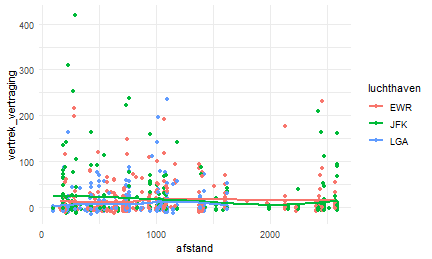
\includegraphics[width=1\linewidth]{textbook_files/figure-latex/labelke2-1} \caption[Vertrekvertraging vs afstand en luchthaven]{Vertrekvertraging vs afstand en luchthaven}\label{fig:labelke2}
\end{figure}

\begin{itemize}
\item
  Geen geweldig resultaat in dit geval.
\item
  Optie 2: Gebruik facetten voor de verschillende luchthavens.
\end{itemize}

\begin{figure*}
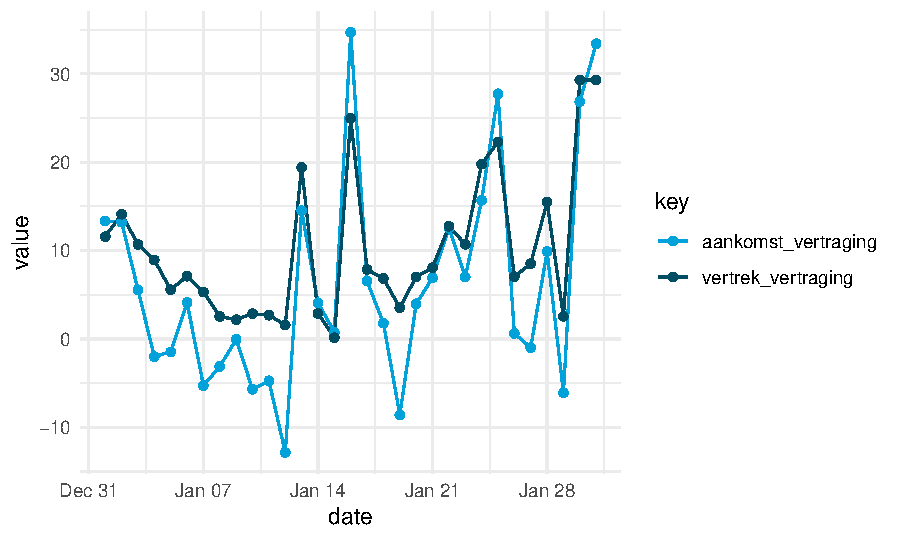
\includegraphics[width=1\linewidth]{textbook_files/figure-latex/unnamed-chunk-22-1} \caption[Vertrekvertraging vs afstand en luchthaven]{Vertrekvertraging vs afstand en luchthaven}\label{fig:unnamed-chunk-22}
\end{figure*}

\begin{itemize}
\tightlist
\item
  Optie 3: Facets, maar gebruik hex bins
\end{itemize}

\begin{figure*}
\includegraphics[width=1\linewidth]{textbook_files/figure-latex/unnamed-chunk-23-1} \caption[Vertrekvertraging vs afstand en luchthaven, hexbins]{Vertrekvertraging vs afstand en luchthaven, hexbins}\label{fig:unnamed-chunk-23}
\end{figure*}

\hypertarget{voorbeeld-multivariaat-tijd}{%
\subsection{Voorbeeld: multivariaat tijd}\label{voorbeeld-multivariaat-tijd}}

\hypertarget{situatie-1-variabelen-hebben-dezelfde-eenheid.}{%
\subsubsection{Situatie 1: Variabelen hebben dezelfde eenheid.}\label{situatie-1-variabelen-hebben-dezelfde-eenheid.}}

Voorbeeld: vertrekvertraging en aankomstvertraging. Je kan lijngrafieken tekenen met meerdere lijnen op hetzelfde assenstelsel.

\begin{figure}
\includegraphics[width=1\linewidth]{textbook_files/figure-latex/unnamed-chunk-24-1} \caption[Evolutie van 2 variabelen over tijd in één grafiek (zelfde meeteenheid)]{Evolutie van 2 variabelen over tijd in één grafiek (zelfde meeteenheid)}\label{fig:unnamed-chunk-24}
\end{figure}

\begin{itemize}
\tightlist
\item
  Of je kan er voor kiezen elke lijn in een afzonderlijk paneel te tonen
\end{itemize}

\begin{figure}
\includegraphics[width=1\linewidth]{textbook_files/figure-latex/unnamed-chunk-25-1} \caption[Evolutie van 2 variabelen over tijd in afzondelijke panels]{Evolutie van 2 variabelen over tijd in afzondelijke panels.}\label{fig:unnamed-chunk-25}
\end{figure}

\hypertarget{situatie-2-variabelen-hebben-niet-dezelfde-eenheid}{%
\subsubsection{Situatie 2: Variabelen hebben niet dezelfde eenheid}\label{situatie-2-variabelen-hebben-niet-dezelfde-eenheid}}

Voorbeeld: de gemiddelde levensverwachting en gdp per capita doorheen de tijd. In dit geval ben je genoodzaakt 2 panelen te gebruiken.

\begin{figure}
\includegraphics[width=1\linewidth]{textbook_files/figure-latex/unnamed-chunk-26-1} \caption[Evolutie van 2 variabelen met andere eenheden in afzonderlijke panels]{Evolutie van 2 variabelen met andere eenheden in afzonderlijke panels.}\label{fig:unnamed-chunk-26}
\end{figure}

Optie 2: Maak een connected scatterplot. Toon een punt voor elke meting, waarbij x en y elk een variabele voorstellen. Verbindt dat elk punt in chronologische volgorde.

\begin{figure}
\includegraphics[width=1\linewidth]{textbook_files/figure-latex/unnamed-chunk-27-1} \caption[Evolutie van 2 variabelen (levensverwachting en inkomen per capita) aan de hand van connected scatterplot]{Evolutie van 2 variabelen (levensverwachting en inkomen per capita) aan de hand van connected scatterplot.}\label{fig:unnamed-chunk-27}
\end{figure}

Variant, per continent:

\begin{figure}
\includegraphics[width=1\linewidth]{textbook_files/figure-latex/unnamed-chunk-28-1} \caption[Evolutie van 2 variabelen aan de hand van connected scatterplot - verschillende groepen]{Evolutie van 2 variabelen aan de hand van connected scatterplot - verschillende groepen.}\label{fig:unnamed-chunk-28}
\end{figure}

\hypertarget{visualisaties-voor-communicatie}{%
\section{Visualisaties voor communicatie}\label{visualisaties-voor-communicatie}}

Wanneer uiteindelijk beslist om een visualizatie te gebruiken om te communiceren, zorg ervoor dat

\begin{itemize}
\tightlist
\item
  de grafiek leesbaar is
\item
  je kleur enkel gebruikt waar nodig.
\item
  je correcte as-labels gebruikt
\item
  je geen theme gebruikt dat te druk/overheersend is
\item
  je een gepaste titel voorziet.
\end{itemize}

\hypertarget{voorbeeld-voor-goed-voor-exploratie}{%
\subsection{Voorbeeld: voor \textasciitilde{} goed voor exploratie}\label{voorbeeld-voor-goed-voor-exploratie}}

\includegraphics[width=1\linewidth]{textbook_files/figure-latex/unnamed-chunk-29-1}

\hypertarget{voorbeeld-na-goed-voor-communicatie}{%
\subsection{Voorbeeld: na \textasciitilde{} goed voor communicatie}\label{voorbeeld-na-goed-voor-communicatie}}

\includegraphics[width=1\linewidth]{textbook_files/figure-latex/unnamed-chunk-30-1}

Merk op: ver van alle grafieken getoond in dit hoofdstuk zijn goed voor communicatie zonder aanpassingen.

\hypertarget{how-charts-lie}{%
\section{How charts lie}\label{how-charts-lie}}

\hypertarget{causaliteit-vs-correlatie}{%
\subsection{Causaliteit vs correlatie}\label{causaliteit-vs-correlatie}}

\begin{itemize}
\tightlist
\item
  Van zodra er twee (or meer) variabelen zijn, gaan we op zoek naar patronen in relaties tussen de variabelen.
\item
  Het is belangrijk en essentieel te beseffen dat mensen een automatische reflex hebben om te denken in termen van oorzaak-gevolg als we kijken naar relaties tussen twee variabelen.

  \begin{itemize}
  \tightlist
  \item
    Het is echter niet omdat er een duidelijke relatie bestaat tussen twee variabelen (correlatie), dat hier sprake is van een oorzaak-gevolg verband (causaliteit).
  \item
    Bijvoorbeeld: Indien in de zomer de verkoop van paraplu's sterk stijgt, dan zal de graanopbrengst in het najaar dalen. Dit betekent niet dat de verkoop van paraplu's een impact heeft op de graanopbrengst. Wat hier waarschijnlijk gebeurt, is dat door hevige regenval in de zomermaanden, de verkoop van paraplu's is toegenomen en de graanoogst tegenvalt.

    \begin{itemize}
    \tightlist
    \item
      Soms is het intuïtief zeer onwaarschijnlijk dat de waargenomen correlatie causaliteit impliceert. Kijk hiervoor maar eens naar de voorbeelden op \url{http://www.tylervigen.com/spurious-correlations}
    \item
      Wanneer het echter plausibel is dat de waargenomen correlatie causaliteit voorstelt, is het belangrijk dat we tegen onze natuurlijke reflex in gaan en niet in termen van oorzaak-gevolg denken.
    \item
      Het aantonen van causaliteit is nooit mogelijk met descriptieve en exploratieve data analyse!
    \end{itemize}
  \end{itemize}
\end{itemize}

\hypertarget{referenties-1}{%
\section{Referenties}\label{referenties-1}}

\begin{itemize}
\tightlist
\item
  \href{https://informationisbeautiful.net/}{Information is Beautiful}
\item
  \href{https://serialmentor.com/dataviz/}{Fundamentals of Data Vizualization}
\item
  \href{https://www.r-graph-gallery.com/}{R Graph Gallery}
\item
  \href{https://www.data-to-viz.com/}{Data to viz}
\item
  \href{https://www.tylervigen.com/spurious-correlations}{Spurrious correlations}
\item
  \href{https://edition.cnn.com/2020/01/17/politics/donald-trump-2016-map-county-by-county/index.html}{Misleading election map}
\end{itemize}

\hypertarget{tutorial---data-vizualisatie}{%
\chapter{Tutorial - Data vizualisatie}\label{tutorial---data-vizualisatie}}

\hypertarget{before-you-start}{%
\section{Before you start}\label{before-you-start}}

Before you start this tutorial, make sure to install the package \texttt{ggplot2}, if you haven't already done so. You can do this using the following line of code:

\begin{Shaded}
\begin{Highlighting}[]
\KeywordTok{install.packages}\NormalTok{(}\StringTok{"ggplot2"}\NormalTok{)}
\end{Highlighting}
\end{Shaded}

In any case, you need to load the package into your session.

\begin{Shaded}
\begin{Highlighting}[]
\KeywordTok{library}\NormalTok{(ggplot2)}
\end{Highlighting}
\end{Shaded}

You also need two datasets, \texttt{movies} and \texttt{diamonds}. Both will be provided as a .RDS file with this tutorial.

\begin{Shaded}
\begin{Highlighting}[]
\NormalTok{movies <-}\StringTok{ }\KeywordTok{readRDS}\NormalTok{(}\StringTok{"movies.RDS"}\NormalTok{)}
\NormalTok{diamonds <-}\StringTok{ }\KeywordTok{readRDS}\NormalTok{(}\StringTok{"diamonds.RDS"}\NormalTok{)}
\end{Highlighting}
\end{Shaded}

\hypertarget{introduction}{%
\section{Introduction}\label{introduction}}

Creating a plot with ggplot2 starts with the \texttt{ggplot()} function. The ggplot function has two important arguments

\begin{itemize}
\tightlist
\item
  \textbf{data}: this will define the dataset to be used for the plot. This must be a data.frame.
\item
  \textbf{mapping}: the mapping will define how the variables are \emph{mapped} onto the aesthetics\footnote{Although it might make certain analyses more interesting when you are familiar with the meaning of the different variables, no specific knowledge about cars is required in order to complete this tutorial.} of the plot, as will be explained further on. This mapping must always be created using the \texttt{aes()} function .
\end{itemize}

For example, we might want to make a scatterplot of the movies in which we use the x-axis for their budget and the y-axis for their rating. We then call ggplot as follows:

\begin{Shaded}
\begin{Highlighting}[]
\KeywordTok{ggplot}\NormalTok{(}\DataTypeTok{data =}\NormalTok{ movies, }\DataTypeTok{mapping =} \KeywordTok{aes}\NormalTok{(}\DataTypeTok{x =}\NormalTok{ budget, }\DataTypeTok{y =}\NormalTok{ rating))}
\end{Highlighting}
\end{Shaded}

\includegraphics[width=1\linewidth]{textbook_files/figure-latex/unnamed-chunk-36-1}

As you can see, this line of code creates a plot with the axes as defined. However, there is no data visualised. The reason herefore is that ggplot doesn't know yet how we want to visualise it. We have to add what is called \emph{a geometric layer}. To create a scatterplot, which consists of \emph{points}, we add \texttt{geom\_point} to the plot.

\begin{Shaded}
\begin{Highlighting}[]
\KeywordTok{ggplot}\NormalTok{(}\DataTypeTok{data =}\NormalTok{ movies, }\DataTypeTok{mapping =} \KeywordTok{aes}\NormalTok{(}\DataTypeTok{x =}\NormalTok{ budget, }\DataTypeTok{y =}\NormalTok{ rating)) }\OperatorTok{+}
\StringTok{    }\KeywordTok{geom_point}\NormalTok{()}
\end{Highlighting}
\end{Shaded}

\includegraphics[width=1\linewidth]{textbook_files/figure-latex/unnamed-chunk-37-1}

This already looks more like it. Remark that the geometric layer was added to the plot by using the \texttt{+} symbol. In this way, multiple layers can be added to the same plot, as well as titles, labels, and configurations of the lay-out, as we will see further on.

Note that we can also place the mapping of the aesthetics in the geometric layer itself. This will make our code slightly more readable for now, as we place the geometric layer and its mapping on the same line.

\begin{Shaded}
\begin{Highlighting}[]
\KeywordTok{ggplot}\NormalTok{(}\DataTypeTok{data =}\NormalTok{ movies) }\OperatorTok{+}
\StringTok{    }\KeywordTok{geom_point}\NormalTok{(}\DataTypeTok{mapping =} \KeywordTok{aes}\NormalTok{(}\DataTypeTok{x =}\NormalTok{ budget, }\DataTypeTok{y =}\NormalTok{ rating))}
\end{Highlighting}
\end{Shaded}

\includegraphics[width=1\linewidth]{textbook_files/figure-latex/unnamed-chunk-38-1}

We have now created our very first plot! In the following sections we will learn how to use different geometrics and aesthetics and how to enhance the layout of our graphs.

\hypertarget{different-geometrics}{%
\section{Different geometrics}\label{different-geometrics}}

Next to \texttt{geom\_point}, many more different geometrics exist to plot data in ggplot. You can check them out by typing `geom\_' in the console and navigating through the auto-completion list. Each of the geom-layers comes with their own specific set of aesthetics that can (and sometimes need to) be mapped. In this tutorial, we will focus mostly on the following geometric layers:

\begin{itemize}
\tightlist
\item
  geom\_point
\item
  geom\_histogram
\item
  geom\_boxplot
\item
  geom\_violin
\item
  geom\_bar
\item
  geom\_col
\end{itemize}

\hypertarget{geom_point}{%
\subsection{geom\_point}\label{geom_point}}

We already used \texttt{geom\_point} to make our first graph, where we mapped two variables on the aesthetics \emph{x} and \emph{y}. However, there are some more aesthetics which can be set using this layer. Let's look at them in more detail.

\begin{itemize}
\tightlist
\item
  \textbf{x}: this will define the position of the points along the x-axis
\item
  \textbf{y}: this will define the position of the points along the y-axis
\item
  \textbf{color}: this will define the color of the points
\item
  \textbf{shape}: this will define the type of points to be plotted\footnote{\includegraphics{images/tidyverse.png} The \emph{tidyverse} is a set of packages for data science that work in harmony because they share common data representations and API design. The \texttt{tidyverse}-package is designed to make it easy to install and load core packages from the tidyverse in a single command. The tidyverse includes packages such as: ggplot2, dplyr, tidyr, readr, purrr, tibble, hms, stringr, lubridate, forcats, jsonlite, readxl, broom, and others. Hadley Wickham can be regarded as the founding father of the tidyverse. The best place to learn about these packages is by reading this book: \href{http://r4ds.had.co.nz/}{R for Data Science}, written by Hadley and Garret Grolemund.}
\item
  \textbf{fill}: this will define how the points are filled (for shapes 21-25)
\item
  \textbf{size}: this will define the size of the points
\item
  \textbf{stroke}: this will define the width of the border
\item
  \textbf{alpha}: this will define the degree of transparancy
\end{itemize}

For example, the graph below will plot black triangles filled with red with a size of 2. Note that the position of the triangles is exactly the same as the position of the points in the previous plot.

\begin{Shaded}
\begin{Highlighting}[]
\KeywordTok{ggplot}\NormalTok{(}\DataTypeTok{data =}\NormalTok{ movies) }\OperatorTok{+}
\StringTok{    }\KeywordTok{geom_point}\NormalTok{(}\DataTypeTok{mapping =} \KeywordTok{aes}\NormalTok{(}\DataTypeTok{x =}\NormalTok{ budget, }\DataTypeTok{y =}\NormalTok{ rating), }
               \DataTypeTok{shape =} \DecValTok{24}\NormalTok{, }
               \DataTypeTok{fill =} \StringTok{"red"}\NormalTok{, }
               \DataTypeTok{color =} \StringTok{"black"}\NormalTok{, }
               \DataTypeTok{size =} \DecValTok{2}\NormalTok{)}
\end{Highlighting}
\end{Shaded}

\includegraphics[width=1\linewidth]{textbook_files/figure-latex/unnamed-chunk-39-1}

But wait, there is something important going on here! While the x and y-aesthetics were defined inside the aes-mapping, the other aesthetics were defined outside of it. Why's that?

Actually, aesthetics can be set in two different ways:

\begin{enumerate}
\def\labelenumi{\arabic{enumi}.}
\tightlist
\item
  They can be \emph{mapped} to a variable in the dataset.
\item
  They can be set to one fixed value.
\end{enumerate}

In our example, x and y are mapped to two variables in the data, i.e.~budget and rating, while the other aesthetics, shape, fill, color and size, are set to fixed values. Although some of the aesthetics typically are always mapped, such as x and y-positions, some others can be a fixed value as well as a mapped variable. For instance, what happens if we map the color of points to a variable, say the variable Action.

\begin{Shaded}
\begin{Highlighting}[]
\KeywordTok{ggplot}\NormalTok{(}\DataTypeTok{data =}\NormalTok{ movies) }\OperatorTok{+}
\StringTok{    }\KeywordTok{geom_point}\NormalTok{(}\DataTypeTok{mapping =} \KeywordTok{aes}\NormalTok{(}\DataTypeTok{x =}\NormalTok{ budget, }
                             \DataTypeTok{y =}\NormalTok{ rating, }
                             \DataTypeTok{color =}\NormalTok{ Action))}
\end{Highlighting}
\end{Shaded}

\includegraphics[width=1\linewidth]{textbook_files/figure-latex/unnamed-chunk-40-1}

We see that points are now colored with respect to the value in the variable Action. Action movies receive a green color, while other movies receive a red color, which we can see in the legend that appeared.

Also the other fixed aesthetics can be used in a mapping. The next example uses the variable Animation for the shape mapping.

\begin{Shaded}
\begin{Highlighting}[]
\KeywordTok{ggplot}\NormalTok{(}\DataTypeTok{data =}\NormalTok{ movies) }\OperatorTok{+}
\StringTok{    }\KeywordTok{geom_point}\NormalTok{(}\DataTypeTok{mapping =} \KeywordTok{aes}\NormalTok{(}\DataTypeTok{x =}\NormalTok{ budget, }
                             \DataTypeTok{y =}\NormalTok{ rating, }
                             \DataTypeTok{color =}\NormalTok{ Action, }
                              \DataTypeTok{shape =}\NormalTok{ Animation))}
\end{Highlighting}
\end{Shaded}

\includegraphics[width=1\linewidth]{textbook_files/figure-latex/unnamed-chunk-41-1}

Great! We now completely understand the geom\_point layer, and the working of the aesthetics-mapping. Now it's time to look at some other geometric layers. We start with histograms.

\hypertarget{geom_histogram}{%
\subsection{geom\_histogram}\label{geom_histogram}}

The \emph{geom\_histogram} layer can be used to plot a histogram. As you should already know, a histogram represents the distribution of \textbf{one} continuous variable. As a result, there is only an x-aesthetic that should be set, and no y-aesthetic. The complete list of aesthetics is as follows:

\begin{itemize}
\tightlist
\item
  \textbf{x}: this will define the variable to be used
\item
  \textbf{color}: this will define the color of the borders
\item
  \textbf{fill}: this will define how the histogram is filled
\item
  \textbf{size}: this will define the size of the border
\item
  \textbf{linetype}: this will define the type of the border \footnote{Note the capital letter I}
\item
  \textbf{alpha}: this will define the degree of transparancy
\item
  \textbf{weight}: this will define how observations should be weigthed. By default, each observation is weigthed as one.
\end{itemize}

Using our knowledge on how to use aesthetics from before, it is now very easy to make a histogram. Let's make a histogram for the rating of movies. We will give it a black border with a white fill. Ready to try?

Let's have a look.

\begin{Shaded}
\begin{Highlighting}[]
\KeywordTok{ggplot}\NormalTok{(movies) }\OperatorTok{+}
\StringTok{    }\KeywordTok{geom_histogram}\NormalTok{(}\KeywordTok{aes}\NormalTok{(rating), }\DataTypeTok{color =} \StringTok{"black"}\NormalTok{, }\DataTypeTok{fill =} \StringTok{"white"}\NormalTok{)}
\end{Highlighting}
\end{Shaded}

\begin{verbatim}
## `stat_bin()` using `bins = 30`. Pick better value with `binwidth`.
\end{verbatim}

\includegraphics[width=1\linewidth]{textbook_files/figure-latex/unnamed-chunk-42-1}

Note that several things were omitted in these two lines of codes. In particular, the argument name \emph{data} in ggplot, \emph{mapping} in geom\_histogram and \emph{x} in aes. Since we know that these are the first arguments of these functions, we can safely omit them, as long as we follow the correct order of arguments. However, we cannot omit \emph{color} and \emph{fill}, as these are not the second and third argument of geom\_histogram. Whenever in doubt, just play safe and write down the proper argument names.

However, that's not the only thing which is tricky here. Indeed, a warning pops up: \texttt{stat\_bin()} using \texttt{bins\ =\ 30}. Pick better value with \texttt{binwidth}. This warning reminds us to the fact that a default value for the number of bins is chosen by geom\_histogram, which is propably not suitable for our graph. We can change the binwidth by adding it as an argument to the geom\_histogram call.

\begin{Shaded}
\begin{Highlighting}[]
\KeywordTok{ggplot}\NormalTok{(movies) }\OperatorTok{+}
\StringTok{    }\KeywordTok{geom_histogram}\NormalTok{(}\KeywordTok{aes}\NormalTok{(rating), }\DataTypeTok{color =} \StringTok{"black"}\NormalTok{, }\DataTypeTok{fill =} \StringTok{"white"}\NormalTok{, }\DataTypeTok{binwidth =} \FloatTok{0.5}\NormalTok{)}
\end{Highlighting}
\end{Shaded}

\includegraphics[width=1\linewidth]{textbook_files/figure-latex/unnamed-chunk-43-1}

Often, the binwidth has an important impact on how the obtained histogram looks like. Carefully configuring this argument by experimenting with different values is therefore important.

In the last plot, we used a fixed color for filling the bars of the histogram. But as we already know by now, we can also map it to a variable in the data. Let's use the variable \emph{Action} one more time.

\begin{Shaded}
\begin{Highlighting}[]
\KeywordTok{ggplot}\NormalTok{(movies) }\OperatorTok{+}
\StringTok{    }\KeywordTok{geom_histogram}\NormalTok{(}\KeywordTok{aes}\NormalTok{(rating, }\DataTypeTok{fill =}\NormalTok{ Action), }\DataTypeTok{color =} \StringTok{"black"}\NormalTok{, }\DataTypeTok{binwidth =} \FloatTok{0.5}\NormalTok{)}
\end{Highlighting}
\end{Shaded}

\includegraphics[width=1\linewidth]{textbook_files/figure-latex/unnamed-chunk-44-1}

Note how we moved the fill argument inside the \texttt{aes}function. Now, each of the bars is filled with two colors: one part for Action movies, and the remainder for other movies. Although it is not very clear in this graph, it appears that the center of the histogram for action movies is slightly more to the left.

Note how the punctuation changes when moving to the aes-mapping: variable names are always used without quotes, i.e.~\emph{bare} variable names, while fixed aesthetics (colors, shapes, linetypes) are used with quotes (except for numbers). It is important to not mess this up!

By default, the histogram for the different \emph{fills} are stacked, i.e.~placed on top of each other. However, we can use the \emph{position} argument of geom\_histogram to put the bars next to each other, or \emph{dodged}.

\begin{Shaded}
\begin{Highlighting}[]
\KeywordTok{ggplot}\NormalTok{(movies) }\OperatorTok{+}
\StringTok{    }\KeywordTok{geom_histogram}\NormalTok{(}\KeywordTok{aes}\NormalTok{(rating, }\DataTypeTok{fill =}\NormalTok{ Action), }
                   \DataTypeTok{color =} \StringTok{"black"}\NormalTok{, }\DataTypeTok{binwidth =} \FloatTok{0.5}\NormalTok{, }\DataTypeTok{position =} \StringTok{"dodge"}\NormalTok{)}
\end{Highlighting}
\end{Shaded}

\includegraphics[width=1\linewidth]{textbook_files/figure-latex/unnamed-chunk-45-1}

Using position = ``dodge'', the bars for Action movies and non-Action movies are placed next to each other, instead of on top of one another. We can go back to the original graph by using position = ``stack'', or just omitting this argument. Later on we will see how to handle such things better by using grids of different plots, or so-called \emph{facets}.

All good so far? Let's look at another way to visualize the distribution of continuous variables, i.e.~the boxplot.

\hypertarget{geom_boxplot}{%
\subsection{geom\_boxplot}\label{geom_boxplot}}

A boxplot places the values of the variable along the y-axis. So, if we want to make a boxplot for ratings, we should use \texttt{aes(y\ =\ ratings)}. However, something tricky is going on here\ldots{} The aesthetics for geom\_boxplot are the following

\begin{itemize}
\tightlist
\item
  \textbf{x}: this will define the variable used for the x-axis
\item
  \textbf{y}: this will define the variable used for the y-axis
\item
  \textbf{color}: this will define the color of the borders
\item
  \textbf{fill}: this will define how the boxplot is filled
\item
  \textbf{size}: this will define the size of the border
\item
  \textbf{linetype}: this will define the type of the border
\item
  \textbf{alpha}: this will define the degree of transparancy
\item
  \textbf{weight}: this will define how observations should be weigthed. By default, each observation is weigthed as one.
\end{itemize}

Thus, the boxplot needs both an x-variable and an y-variable? That seems strange at first sight. The reason behind this is that in the philosophy of ggplot, always \emph{something} must be plot on both x and y-axes. Although only a x-variable is given to a histogram, it will compute frequencies to plot on the y-axis. However, there is no such thing going to happen for boxplots. As a result, the x-axis should be used to map different categories for which the distribution can then be compared. For instance, we can compare the rating for Action movies with those for other movies.

\begin{Shaded}
\begin{Highlighting}[]
\KeywordTok{ggplot}\NormalTok{(movies) }\OperatorTok{+}\StringTok{ }
\StringTok{    }\KeywordTok{geom_boxplot}\NormalTok{(}\KeywordTok{aes}\NormalTok{(Action, rating))}
\end{Highlighting}
\end{Shaded}

\includegraphics[width=1\linewidth]{textbook_files/figure-latex/unnamed-chunk-46-1}

Here we see that, as we already suspected, Action movies tend to have a lower rating compared to other movies. We can change the color and the fill of the boxplot just like before, as well as the linetype, the size of the border, or the transparency.

But, what if we just want to plot a boxplot of the overal rating, without having to specify a variable for the x-axis? A little workaround is needed here. One possibility is to use an \emph{empty string} for the x-axis mapping.

\begin{Shaded}
\begin{Highlighting}[]
\KeywordTok{ggplot}\NormalTok{(movies) }\OperatorTok{+}
\StringTok{    }\KeywordTok{geom_boxplot}\NormalTok{(}\KeywordTok{aes}\NormalTok{(}\StringTok{""}\NormalTok{, rating))}
\end{Highlighting}
\end{Shaded}

\includegraphics[width=1\linewidth]{textbook_files/figure-latex/unnamed-chunk-47-1}

Note that this creates the label ``x'' for the x-axis, where we would normally find the name of the variable mapped onto it. Later we will see how to omit this label to make our graph a little nicer.

\hypertarget{geom_violin}{%
\subsection{geom\_violin}\label{geom_violin}}

The violin-plot is similar to the boxplot, although it will reflect in more detail where the mass of the values is located. Its aesthetics are the same as for a boxplot.

\begin{itemize}
\tightlist
\item
  \textbf{x}: this will define the variable used for the x-axis
\item
  \textbf{y}: this will define the variable used for the y-axis
\item
  \textbf{color}: this will define the color of the borders
\item
  \textbf{fill}: this will define how the violin is filled
\item
  \textbf{size}: this will define the size of the border
\item
  \textbf{linetype}: this will define the type of the border
\item
  \textbf{alpha}: this will define the degree of transparency
\item
  \textbf{weight}: this will define how observations should be weighted. By default, each observation is weigthed as one.
\end{itemize}

Let's make the same graphs, now using the violin-plot.

\begin{Shaded}
\begin{Highlighting}[]
\KeywordTok{ggplot}\NormalTok{(movies) }\OperatorTok{+}\StringTok{ }
\StringTok{    }\KeywordTok{geom_violin}\NormalTok{(}\KeywordTok{aes}\NormalTok{(Action, rating))}
\end{Highlighting}
\end{Shaded}

\includegraphics[width=1\linewidth]{textbook_files/figure-latex/unnamed-chunk-48-1}

It's probably clear now where this type of graph got its name from. As you can see, violin plots somehow sit in between boxplots and histograms. However, since their width is normalized, they can be used better for comparison. Also here, we can use the same workaround if we want to plot the overal distribution.

\begin{Shaded}
\begin{Highlighting}[]
\KeywordTok{ggplot}\NormalTok{(movies) }\OperatorTok{+}
\StringTok{    }\KeywordTok{geom_violin}\NormalTok{(}\KeywordTok{aes}\NormalTok{(}\StringTok{""}\NormalTok{, rating))}
\end{Highlighting}
\end{Shaded}

\includegraphics[width=1\linewidth]{textbook_files/figure-latex/unnamed-chunk-49-1}

So far, we have seen three different ways to analyse the distribution of continuous variables. Now, we will look into barplots, which can be used to represent categorical distribution.

\hypertarget{geom_bar}{%
\subsection{geom\_bar}\label{geom_bar}}

Just like a histogram, a barplot only needs an x variable. The difference is that this variable needs to be categorical, while for histograms it needs to be continuous. The full list of aesthetics is the following:

\begin{itemize}
\tightlist
\item
  \textbf{x}: this will define the variable used for the x-axis
\item
  \textbf{color}: this will define the color of the borders
\item
  \textbf{fill}: this will define how the bars are filled
\item
  \textbf{size}: this will define the size of the border
\item
  \textbf{linetype}: this will define the type of the border
\item
  \textbf{alpha}: this will define the degree of transparency
\item
  \textbf{weight}: this will define how observations should be weigthed. By default, each observation is weigthed as one.
\end{itemize}

We can make a simple bar chart that shows how many Action movies there are, and how many other movies, as follows.

\begin{Shaded}
\begin{Highlighting}[]
\KeywordTok{ggplot}\NormalTok{(movies) }\OperatorTok{+}
\StringTok{    }\KeywordTok{geom_bar}\NormalTok{(}\KeywordTok{aes}\NormalTok{(Action))}
\end{Highlighting}
\end{Shaded}

\includegraphics[width=1\linewidth]{textbook_files/figure-latex/unnamed-chunk-50-1}

Furthermore, we could add colors to this, according to the number of Animation movies. We immediately see that there are almost no Action movies which are also animation movies.

\begin{Shaded}
\begin{Highlighting}[]
\KeywordTok{ggplot}\NormalTok{(movies) }\OperatorTok{+}
\StringTok{    }\KeywordTok{geom_bar}\NormalTok{(}\KeywordTok{aes}\NormalTok{(Action, }\DataTypeTok{fill =}\NormalTok{ Animation)) }
\end{Highlighting}
\end{Shaded}

\includegraphics[width=1\linewidth]{textbook_files/figure-latex/unnamed-chunk-51-1}

We can do the same for Romance and Comedy movies.

\begin{Shaded}
\begin{Highlighting}[]
\KeywordTok{ggplot}\NormalTok{(movies) }\OperatorTok{+}
\StringTok{    }\KeywordTok{geom_bar}\NormalTok{(}\KeywordTok{aes}\NormalTok{(Romance, }\DataTypeTok{fill =}\NormalTok{ Comedy)) }
\end{Highlighting}
\end{Shaded}

\includegraphics[width=1\linewidth]{textbook_files/figure-latex/unnamed-chunk-52-1}

In contrast, it can be seen here that approximately half of the Romantic movies are also comedy, which is more compared to non-romantic movies.

Remember that, in case of histograms, we could change the position to ``dodge'', which placed the bars next to each other. The same can be done here.

\begin{Shaded}
\begin{Highlighting}[]
\KeywordTok{ggplot}\NormalTok{(movies) }\OperatorTok{+}
\StringTok{    }\KeywordTok{geom_bar}\NormalTok{(}\KeywordTok{aes}\NormalTok{(Romance, }\DataTypeTok{fill =}\NormalTok{ Comedy), }\DataTypeTok{position =} \StringTok{"dodge"}\NormalTok{) }
\end{Highlighting}
\end{Shaded}

\includegraphics[width=1\linewidth]{textbook_files/figure-latex/unnamed-chunk-53-1}

A third option that is available for the position is to extend the bars so that they have the same height. As a result, we will observe the distribution of values as a part of a whole. Instead of the count, the labels on the y-axis will now depict the percentage points.

\begin{Shaded}
\begin{Highlighting}[]
\KeywordTok{ggplot}\NormalTok{(movies) }\OperatorTok{+}
\StringTok{    }\KeywordTok{geom_bar}\NormalTok{(}\KeywordTok{aes}\NormalTok{(Romance, }\DataTypeTok{fill =}\NormalTok{ Comedy), }\DataTypeTok{position =} \StringTok{"fill"}\NormalTok{) }
\end{Highlighting}
\end{Shaded}

\includegraphics[width=1\linewidth]{textbook_files/figure-latex/unnamed-chunk-54-1}

Finally, if we want to do this to show the distribution of one variable, we can use the same workaround as before and set the x-aesthetic to "". The plot below will show the portion of all movies that are comedies.\footnote{Note that in cases like these, it perfectly makes sense to make the plot less wide, or flip it 90 degrees and make it less high. However, these are configurations related to the output devices used, and we will not consider them here.}

\begin{Shaded}
\begin{Highlighting}[]
\KeywordTok{ggplot}\NormalTok{(movies) }\OperatorTok{+}
\StringTok{    }\KeywordTok{geom_bar}\NormalTok{(}\KeywordTok{aes}\NormalTok{(}\StringTok{""}\NormalTok{, }\DataTypeTok{fill =}\NormalTok{ Comedy), }\DataTypeTok{position =} \StringTok{"fill"}\NormalTok{) }
\end{Highlighting}
\end{Shaded}

\includegraphics[width=1\linewidth]{textbook_files/figure-latex/unnamed-chunk-55-1}

\hypertarget{geom_col}{%
\subsection{geom\_col}\label{geom_col}}

When we use geom\_bar, the heights of the bars are computed by using the frequency of the categorical variable. However, sometimes we just want to plot a bar chart with values that are already in the data, or values which we computed ourselves. For instance, what if we wanted a barchart depicting the budget of a set of movies? In such a case, we can use \emph{geom\_col}. ``Col'' indicates that we want to use a column in the data to set the height of the bars. The aesthetics are the same for geom\_bar, only now we need to specify a variable for the y-axis, evidently.

\begin{itemize}
\tightlist
\item
  \textbf{x}: this will define the variable used for the x-axis
\item
  \textbf{y}: this will define the variable used for the y-axis
\item
  \textbf{color}: this will define the color of the borders
\item
  \textbf{fill}: this will define how the bars are filled
\item
  \textbf{size}: this will define the size of the border
\item
  \textbf{linetype}: this will define the type of the border
\item
  \textbf{alpha}: this will define the degree of transparency
\item
  \textbf{weight}: this will define how observations should be weigthed. By default, each observation is weigthed as one.
\end{itemize}

Let's make a barplot depicting the budget of all movies from 2004 where the budget was higher than 100 million.

\begin{Shaded}
\begin{Highlighting}[]
\KeywordTok{filter}\NormalTok{(movies, year }\OperatorTok{==}\StringTok{ }\DecValTok{2004}\NormalTok{, budget }\OperatorTok{>}\StringTok{ }\DecValTok{100000000}\NormalTok{) }\OperatorTok
\StringTok{    }\KeywordTok{ggplot}\NormalTok{() }\OperatorTok{+}
\StringTok{    }\KeywordTok{geom_col}\NormalTok{(}\KeywordTok{aes}\NormalTok{(title, budget))}
\end{Highlighting}
\end{Shaded}

\includegraphics[width=1\linewidth]{textbook_files/figure-latex/unnamed-chunk-56-1}

Do you notice something strange in the code? Don't worry if you don't understand the first line. All you need to know is that we filtered movies from 2004 with a budget higher than 100 million. The strange looking \%\textgreater\% symbol will make sure this data is passed to ggplot. We will come back to this in another session. \footnote{\includegraphics{images/pipe.jpg} The piping symbol was first introduced in the package \texttt{magrittr}, evidently named after the Belgian surrealist artist René Magritte, well-known for his painting \emph{The Threachery of Images}, aka \emph{Ceci n'est pas un pipe}.}

We have now plotted movie titles on the x-axis and budget on the y-axis. Great! Or not so? The values on the x-asis are somewhat cluttered and unreadable. It's time now to give some attention to the layout of our plots!

\hypertarget{other-geometrics}{%
\subsection{Other geometrics}\label{other-geometrics}}

So far, we used the most important geometrics to make simple visualizations: scatterplots, histograms, boxplots, violinplots and bar plots. However, we only covered the tip of the iceberg, as many more types exist, some simple and some more advanced. An overview of all geoms and their uses can be found in the \href{https://www.rstudio.com/wp-content/uploads/2015/12/ggplot2-cheatsheet-2.0.pdf}{ggplot Cheat Sheet}, of which an extract is shown here. Don't be afraid to try something out!

\includegraphics{images/geoms.PNG}

\hypertarget{enhancing-the-appearance-of-our-plots}{%
\section{Enhancing the appearance of our plots}\label{enhancing-the-appearance-of-our-plots}}

So far, we have mainly looked at different types of plots and how to map them on our data. In this section, we will focus on the presentation of the plot, e.g.~titles, colors, axes, etc. The concepts introduced in this section can be applied for any type of plot, no matter which geometric object is used.

In this section, the dataset ``diamonds'' will be used. The plot below will be used as a starting point. \footnote{The table of a diamond refers to the flat facet of the diamond which can be seen when the stone is faced up. The depth of a diamond is its height (in millimeters) measured from the culet to the table.}

\begin{Shaded}
\begin{Highlighting}[]
\KeywordTok{ggplot}\NormalTok{(diamonds) }\OperatorTok{+}
\StringTok{    }\KeywordTok{geom_point}\NormalTok{(}\KeywordTok{aes}\NormalTok{(table, depth, }\DataTypeTok{color =}\NormalTok{ cut))}
\end{Highlighting}
\end{Shaded}

\includegraphics[width=1\linewidth]{textbook_files/figure-latex/unnamed-chunk-57-1}

\hypertarget{titles}{%
\subsection{Titles}\label{titles}}

One of the most important things to add to our plot are titles. Titles are used to give meaning to the axis as well as the plot itself. The most straightforward way to add titles is to use the function \texttt{labs()}. In this function, 4 arguments can be set: the title, the subtitle, x for the x label and y for the y label. The labs function can just be added to the plot as an extra layer.

\begin{Shaded}
\begin{Highlighting}[]
\KeywordTok{data}\NormalTok{(}\StringTok{"diamonds"}\NormalTok{)}
\KeywordTok{ggplot}\NormalTok{(diamonds) }\OperatorTok{+}
\StringTok{    }\KeywordTok{geom_point}\NormalTok{(}\KeywordTok{aes}\NormalTok{(table, depth, }\DataTypeTok{color =}\NormalTok{ cut)) }\OperatorTok{+}\StringTok{ }
\StringTok{    }\KeywordTok{labs}\NormalTok{(}\DataTypeTok{title =} \StringTok{"Comparing table and depth of diamonds"}\NormalTok{,}
         \DataTypeTok{subtitle =} \StringTok{"What combination of table and depth gives good quality diamonds?"}\NormalTok{,}
         \DataTypeTok{x =} \StringTok{"Table"}\NormalTok{,}
         \DataTypeTok{y =} \StringTok{"Depth"}\NormalTok{)}
\end{Highlighting}
\end{Shaded}

\includegraphics[width=1\linewidth]{textbook_files/figure-latex/unnamed-chunk-58-1}

You'll see that our graph already looks much better when titles are added! However, there is much more to improve.

\hypertarget{theme}{%
\subsection{Theme}\label{theme}}

The \emph{theme} of a plot defines its overall appearance: the gridlines, the background, the size of the text, titles and legend, the position of the legend, etc. The theme can be defined manually by adding a \texttt{theme()} layer to the plot and by setting the required arguments. (You can look at ?theme to see the arguments which are avaibable). However, this is a cumbersome approach. Fortunately, some predefined themes are provided in ggplot:

\begin{itemize}
\tightlist
\item
  \textbf{theme\_gray}: the default theme (used so far)
\item
  \textbf{theme\_bw}: a theme for black-white plots
\item
  \textbf{theme\_dark}: a dark theme for contrast
\item
  \textbf{theme\_classic}: a minimal theme
\item
  \textbf{theme\_light}: another minimal theme
\item
  \textbf{theme\_linedraw}: yet another minimal theme
\item
  \textbf{theme\_minimal}: yet another minimal theme
\item
  \textbf{theme\_void}: an empty theme
\end{itemize}

Feel free to experiment with some of these themes. Preferably, you can use some of the minimal themes. Here, we used the theme\_light theme. \footnote{For most of the layers, it is not important in which order they are added to a plot. However, if you make manual changes with \texttt{theme}, make sure to put them after any predefined theme, otherwise your changes will be overwritten.}

\begin{Shaded}
\begin{Highlighting}[]
\KeywordTok{ggplot}\NormalTok{(diamonds) }\OperatorTok{+}
\StringTok{    }\KeywordTok{geom_point}\NormalTok{(}\KeywordTok{aes}\NormalTok{(table, depth, }\DataTypeTok{color =}\NormalTok{ cut)) }\OperatorTok{+}\StringTok{ }
\StringTok{    }\KeywordTok{labs}\NormalTok{(}\DataTypeTok{title =} \StringTok{"Comparing table and depth of diamonds"}\NormalTok{,}
         \DataTypeTok{subtitle =} \StringTok{"What combination of table and depth gives good quality diamonds?"}\NormalTok{,}
         \DataTypeTok{x =} \StringTok{"Table"}\NormalTok{,}
         \DataTypeTok{y =} \StringTok{"Depth"}\NormalTok{) }\OperatorTok{+}
\StringTok{    }\KeywordTok{theme_light}\NormalTok{()}
\end{Highlighting}
\end{Shaded}

\includegraphics[width=1\linewidth]{textbook_files/figure-latex/unnamed-chunk-59-1}

When you are not yet satisfied with any of these themes, you can install the package \texttt{ggthemes} to get hold of even more themes, such as the theme from \emph{The Economist}, \emph{fivethirtyeight.com}, or \emph{Google Docs}.

\hypertarget{configuring-the-coordinate-system}{%
\subsection{Configuring the coordinate system}\label{configuring-the-coordinate-system}}

The appearance of the graph is not only defined by the titles and the graphics. Also the axes in the coordinate system need some attention. One thing to decide on are the limits of the coordinate system. This can be done using the function \texttt{coord\_cartesian} and its arguments \emph{xlim} and \emph{ylim}. Both arguments expect a numerical vector of length two. Let's see how this works in our example. \footnote{A Cartesian coordinate system is a coordinate system that specifies each point uniquely in a plane by a pair of numerical coordinates, which are the signed distances to the point from two fixed perpendicular directed lines, measured in the same unit of length.}

\begin{Shaded}
\begin{Highlighting}[]
\KeywordTok{ggplot}\NormalTok{(diamonds) }\OperatorTok{+}
\StringTok{    }\KeywordTok{geom_point}\NormalTok{(}\KeywordTok{aes}\NormalTok{(table, depth, }\DataTypeTok{color =}\NormalTok{ cut)) }\OperatorTok{+}\StringTok{ }
\StringTok{    }\KeywordTok{labs}\NormalTok{(}\DataTypeTok{title =} \StringTok{"Comparing table and depth of diamonds"}\NormalTok{,}
         \DataTypeTok{subtitle =} \StringTok{"What combination of table and depth gives good quality diamonds?"}\NormalTok{,}
         \DataTypeTok{x =} \StringTok{"Table"}\NormalTok{,}
         \DataTypeTok{y =} \StringTok{"Depth"}\NormalTok{) }\OperatorTok{+}
\StringTok{    }\KeywordTok{theme_light}\NormalTok{() }\OperatorTok{+}
\StringTok{    }\KeywordTok{coord_cartesian}\NormalTok{(}\DataTypeTok{xlim =} \KeywordTok{c}\NormalTok{(}\DecValTok{45}\NormalTok{,}\DecValTok{75}\NormalTok{), }\DataTypeTok{ylim =} \KeywordTok{c}\NormalTok{(}\DecValTok{50}\NormalTok{, }\DecValTok{75}\NormalTok{))}
\end{Highlighting}
\end{Shaded}

\includegraphics[width=1\linewidth]{textbook_files/figure-latex/unnamed-chunk-60-1}

We have now limited the x-axis to the interval from 45 to 75, while we have limited the y-axis to the interval 50 to 75. There are some alternatives to the cartesian coordinate system which are less often used. Notable ones are:

\begin{itemize}
\tightlist
\item
  coord\_equal: a coordinate system where the x-axis and y-axis are scaled equally (i.e.~ration = 1)
\item
  coord\_fixed: a coordinate system with a fixed ratio
\item
  coord\_polar: a coordinate system for polar plots, or pie charts
\item
  coord\_map: a coordinate system for plotting geographical data.
\end{itemize}

Next to setting the limits of the coordinate system, we can also set the breaks on the x-axis and y-axis. This can be done using the functions \texttt{scale\_x\_continuous} and \texttt{scale\_y\_continuous} respectively. Both functions have a \emph{breaks} argument. This argument can be given a vector of values to be plot as labels on the axis.\footnote{Note that the scale\_.\_continuous functions also have an argument \texttt{limits} to set the limits of the axes which can be used instead of coord\_cartesion. However, there is a tricky difference. Coord\_cartesian will zoom into the limits withouth throwing away other data points. Setting the limits within the scale functions, however, will throw away data points and can bias your visualisation. \includegraphics{images/zoom.png}} We can use the function \texttt{seq} to create this vector: i.e.~\texttt{seq(0,10,5)} will return a vector starting at 0 and increasing to ten with intervals of 5. \footnote{The titles of the axes which we defined with the \texttt{labs} function can also be set in the scale functions with the argument \texttt{name}. As you get more familiar with using ggplot2, you will often find that there are multiple ways to reach the same goal.}

\begin{Shaded}
\begin{Highlighting}[]
\KeywordTok{ggplot}\NormalTok{(diamonds) }\OperatorTok{+}
\StringTok{    }\KeywordTok{geom_point}\NormalTok{(}\KeywordTok{aes}\NormalTok{(table, depth, }\DataTypeTok{color =}\NormalTok{ cut)) }\OperatorTok{+}\StringTok{ }
\StringTok{    }\KeywordTok{labs}\NormalTok{(}\DataTypeTok{title =} \StringTok{"Comparing table and depth of diamonds"}\NormalTok{,}
         \DataTypeTok{subtitle =} \StringTok{"What combination of table}
\StringTok{         and depth gives good quality diamonds?"}\NormalTok{,}
         \DataTypeTok{x =} \StringTok{"Table"}\NormalTok{,}
         \DataTypeTok{y =} \StringTok{"Depth"}\NormalTok{) }\OperatorTok{+}
\StringTok{    }\KeywordTok{theme_light}\NormalTok{() }\OperatorTok{+}
\StringTok{    }\KeywordTok{coord_cartesian}\NormalTok{(}\DataTypeTok{xlim =} \KeywordTok{c}\NormalTok{(}\DecValTok{45}\NormalTok{,}\DecValTok{75}\NormalTok{), }\DataTypeTok{ylim =} \KeywordTok{c}\NormalTok{(}\DecValTok{50}\NormalTok{, }\DecValTok{75}\NormalTok{)) }\OperatorTok{+}
\StringTok{    }\KeywordTok{scale_x_continuous}\NormalTok{(}\DataTypeTok{breaks =} \KeywordTok{seq}\NormalTok{(}\DecValTok{45}\NormalTok{,}\DecValTok{75}\NormalTok{,}\DecValTok{5}\NormalTok{)) }\OperatorTok{+}
\StringTok{    }\KeywordTok{scale_y_continuous}\NormalTok{(}\DataTypeTok{breaks =} \KeywordTok{seq}\NormalTok{(}\DecValTok{50}\NormalTok{,}\DecValTok{75}\NormalTok{,}\DecValTok{5}\NormalTok{))}
\end{Highlighting}
\end{Shaded}

\includegraphics[width=1\linewidth]{textbook_files/figure-latex/unnamed-chunk-61-1}

Another useful function is the \texttt{coord\_flip} function, which we will illustrate with the following graph we saw earlier.

\begin{Shaded}
\begin{Highlighting}[]
\KeywordTok{filter}\NormalTok{(movies, year }\OperatorTok{==}\StringTok{ }\DecValTok{2004}\NormalTok{, budget }\OperatorTok{>}\StringTok{ }\DecValTok{100000000}\NormalTok{) }\OperatorTok
\StringTok{    }\KeywordTok{ggplot}\NormalTok{() }\OperatorTok{+}
\StringTok{    }\KeywordTok{geom_col}\NormalTok{(}\KeywordTok{aes}\NormalTok{(title, budget))}
\end{Highlighting}
\end{Shaded}

\includegraphics[width=1\linewidth]{textbook_files/figure-latex/unnamed-chunk-62-1}

As you may remember, the movie titles on the x-axis were overlapping and therefore unreadable. One way to fix this is to \emph{flip} the entire graph, such that the labels of the x-asis are placed on the y-axis, and can be read horizontally.

\begin{Shaded}
\begin{Highlighting}[]
\KeywordTok{filter}\NormalTok{(movies, year }\OperatorTok{==}\StringTok{ }\DecValTok{2004}\NormalTok{, budget }\OperatorTok{>}\StringTok{ }\DecValTok{100000000}\NormalTok{) }\OperatorTok
\StringTok{    }\KeywordTok{ggplot}\NormalTok{() }\OperatorTok{+}
\StringTok{    }\KeywordTok{geom_col}\NormalTok{(}\KeywordTok{aes}\NormalTok{(title, budget)) }\OperatorTok{+}
\StringTok{    }\KeywordTok{coord_flip}\NormalTok{()}
\end{Highlighting}
\end{Shaded}

\includegraphics[width=1\linewidth]{textbook_files/figure-latex/unnamed-chunk-63-1}

Another option is to keep the original orientation, but the change the orientation of the labels on the x-axis. You could rotate them by 45 or 90 degrees, for instance. This can be done with the \texttt{theme} function. Ready to experiment? Challenge yourself!

As our code contains more and more lines, our plot is getting nicer and nicer! Good job! The last thing on our list are colors.

\hypertarget{color-scales}{%
\subsection{Color scales}\label{color-scales}}

Often, we use color or fill to visualise categorical data, such as the quality of the cut in our graph about diamonds. By default, ggplot will use a rainbow theme. However, many more palettes are available. We can add these by using \texttt{scale\_color\_brewer} or \texttt{scale\_fill\_brewer}, depending on whether it concerns a color or fill-color. Both layers have a palette argument, of which the possible values can be found below.

\begin{figure}
\centering
\includegraphics{images/brewer-pal.png}
\caption{R color palettes}
\end{figure}

For instance, let's use the Set1 pallete.

\begin{Shaded}
\begin{Highlighting}[]
\KeywordTok{ggplot}\NormalTok{(diamonds) }\OperatorTok{+}
\StringTok{    }\KeywordTok{geom_point}\NormalTok{(}\KeywordTok{aes}\NormalTok{(table, depth, }\DataTypeTok{col =}\NormalTok{ cut)) }\OperatorTok{+}\StringTok{ }
\StringTok{    }\KeywordTok{labs}\NormalTok{(}\DataTypeTok{title =} \StringTok{"Comparing table and depth of diamonds"}\NormalTok{,}
         \DataTypeTok{subtitle =} \StringTok{"What combination of table and depth gives good quality diamonds?"}\NormalTok{,}
         \DataTypeTok{x =} \StringTok{"Table"}\NormalTok{,}
         \DataTypeTok{y =} \StringTok{"Depth"}\NormalTok{) }\OperatorTok{+}
\StringTok{    }\KeywordTok{theme_light}\NormalTok{() }\OperatorTok{+}
\StringTok{    }\KeywordTok{coord_cartesian}\NormalTok{(}\DataTypeTok{xlim =} \KeywordTok{c}\NormalTok{(}\DecValTok{45}\NormalTok{,}\DecValTok{75}\NormalTok{), }\DataTypeTok{ylim =} \KeywordTok{c}\NormalTok{(}\DecValTok{50}\NormalTok{, }\DecValTok{75}\NormalTok{)) }\OperatorTok{+}
\StringTok{    }\KeywordTok{scale_x_continuous}\NormalTok{(}\DataTypeTok{breaks =} \KeywordTok{seq}\NormalTok{(}\DecValTok{45}\NormalTok{,}\DecValTok{75}\NormalTok{,}\DecValTok{5}\NormalTok{)) }\OperatorTok{+}
\StringTok{    }\KeywordTok{scale_y_continuous}\NormalTok{(}\DataTypeTok{breaks =} \KeywordTok{seq}\NormalTok{(}\DecValTok{50}\NormalTok{,}\DecValTok{75}\NormalTok{,}\DecValTok{5}\NormalTok{)) }\OperatorTok{+}
\StringTok{    }\KeywordTok{scale_color_brewer}\NormalTok{(}\DataTypeTok{palette =} \StringTok{"Set1"}\NormalTok{)}
\end{Highlighting}
\end{Shaded}

\includegraphics[width=1\linewidth]{textbook_files/figure-latex/unnamed-chunk-64-1}

The scale\_.\_brewer functions also have the argument \texttt{name}, which we can use to set the name of the legend, and the argument \texttt{guide}, which will remove the legend if set to FALSE.

\begin{Shaded}
\begin{Highlighting}[]
\KeywordTok{ggplot}\NormalTok{(diamonds) }\OperatorTok{+}
\StringTok{    }\KeywordTok{geom_point}\NormalTok{(}\KeywordTok{aes}\NormalTok{(table, depth, }\DataTypeTok{col =}\NormalTok{ cut)) }\OperatorTok{+}\StringTok{ }
\StringTok{    }\KeywordTok{labs}\NormalTok{(}\DataTypeTok{title =} \StringTok{"Comparing table and depth of diamonds"}\NormalTok{,}
         \DataTypeTok{subtitle =} \StringTok{"What combination of table and depth gives good quality diamonds?"}\NormalTok{,}
         \DataTypeTok{x =} \StringTok{"Table"}\NormalTok{,}
         \DataTypeTok{y =} \StringTok{"Depth"}\NormalTok{) }\OperatorTok{+}
\StringTok{    }\KeywordTok{theme_light}\NormalTok{() }\OperatorTok{+}
\StringTok{    }\KeywordTok{coord_cartesian}\NormalTok{(}\DataTypeTok{xlim =} \KeywordTok{c}\NormalTok{(}\DecValTok{45}\NormalTok{,}\DecValTok{75}\NormalTok{), }\DataTypeTok{ylim =} \KeywordTok{c}\NormalTok{(}\DecValTok{50}\NormalTok{, }\DecValTok{75}\NormalTok{)) }\OperatorTok{+}
\StringTok{    }\KeywordTok{scale_x_continuous}\NormalTok{(}\DataTypeTok{breaks =} \KeywordTok{seq}\NormalTok{(}\DecValTok{45}\NormalTok{,}\DecValTok{75}\NormalTok{,}\DecValTok{5}\NormalTok{)) }\OperatorTok{+}
\StringTok{    }\KeywordTok{scale_y_continuous}\NormalTok{(}\DataTypeTok{breaks =} \KeywordTok{seq}\NormalTok{(}\DecValTok{50}\NormalTok{,}\DecValTok{75}\NormalTok{,}\DecValTok{5}\NormalTok{)) }\OperatorTok{+}
\StringTok{    }\KeywordTok{scale_color_brewer}\NormalTok{(}\DataTypeTok{palette =} \StringTok{"Set1"}\NormalTok{, }\DataTypeTok{name =} \StringTok{"Diamond Cut Quality"}\NormalTok{)}
\end{Highlighting}
\end{Shaded}

\includegraphics[width=1\linewidth]{textbook_files/figure-latex/unnamed-chunk-65-1}

Next to the standard color palettes avaiable, many more can be found in the packages \texttt{ggthemes} and \texttt{ggsci}. They can be used by adding \emph{scale\_color}+ name of the palette. Feel free to explore some more!

\hypertarget{advanced-plots}{%
\section{Advanced plots}\label{advanced-plots}}

Often, you want to compare plots for different categories of a variable. In our example, we looked for which combinations of table and depth, the cut of the diamond was good. We now want to know whether there is a difference between the 8 different clarity levels in the data. One way would be to make 8 different plots, one for each of the levels. However, this would be cumbersome to put together. Fortunately, we can use the function \texttt{facet\_grid} to create different plots within a plot.

\hypertarget{using-facets}{%
\subsection{Using Facets}\label{using-facets}}

This function expects a formula in the form of \texttt{A\ \textasciitilde{}\ B} where A and B are two categorical variables. For each combination of values of A and B, a different plot will be constructed, and they will be arranged in a grid where the values of A each constitute a row and the values of B each constitute a column. Comparisons of more than 2 variables are possible using a formula of the form \texttt{A\ +\ B\ \textasciitilde{}\ C}. A comparison along one variable is possible by using a dot instead of a variable name, i.e.~\texttt{.\ \textasciitilde{}\ A} or \texttt{A\ \textasciitilde{}\ .} .

In the following plot, we use facets to redraw our plot for each of the clarity levels. Furthermore, the legend is placed on top to create more space.

\begin{Shaded}
\begin{Highlighting}[]
\KeywordTok{ggplot}\NormalTok{(diamonds) }\OperatorTok{+}
\StringTok{    }\KeywordTok{geom_point}\NormalTok{(}\KeywordTok{aes}\NormalTok{(table, depth, }\DataTypeTok{col =}\NormalTok{ cut)) }\OperatorTok{+}\StringTok{ }
\StringTok{    }\KeywordTok{labs}\NormalTok{(}\DataTypeTok{title =} \StringTok{"Comparing table and depth of diamonds"}\NormalTok{,}
         \DataTypeTok{subtitle =} \StringTok{"What combination of table and depth gives good quality diamonds?"}\NormalTok{,}
         \DataTypeTok{x =} \StringTok{"Table"}\NormalTok{,}
         \DataTypeTok{y =} \StringTok{"Depth"}\NormalTok{) }\OperatorTok{+}
\StringTok{    }\KeywordTok{theme_light}\NormalTok{() }\OperatorTok{+}
\StringTok{    }\KeywordTok{coord_cartesian}\NormalTok{(}\DataTypeTok{xlim =} \KeywordTok{c}\NormalTok{(}\DecValTok{45}\NormalTok{,}\DecValTok{75}\NormalTok{), }\DataTypeTok{ylim =} \KeywordTok{c}\NormalTok{(}\DecValTok{50}\NormalTok{, }\DecValTok{75}\NormalTok{)) }\OperatorTok{+}
\StringTok{    }\KeywordTok{scale_x_continuous}\NormalTok{(}\DataTypeTok{breaks =} \KeywordTok{seq}\NormalTok{(}\DecValTok{45}\NormalTok{,}\DecValTok{75}\NormalTok{,}\DecValTok{5}\NormalTok{)) }\OperatorTok{+}
\StringTok{    }\KeywordTok{scale_y_continuous}\NormalTok{(}\DataTypeTok{breaks =} \KeywordTok{seq}\NormalTok{(}\DecValTok{50}\NormalTok{,}\DecValTok{75}\NormalTok{,}\DecValTok{5}\NormalTok{)) }\OperatorTok{+}
\StringTok{    }\KeywordTok{scale_color_brewer}\NormalTok{(}\DataTypeTok{palette =} \StringTok{"Set1"}\NormalTok{, }\DataTypeTok{name =} \StringTok{"Diamond Cut Quality"}\NormalTok{) }\OperatorTok{+}
\StringTok{    }\KeywordTok{facet_grid}\NormalTok{(. }\OperatorTok{~}\StringTok{ }\NormalTok{clarity) }\OperatorTok{+}
\StringTok{    }\KeywordTok{theme}\NormalTok{(}\DataTypeTok{legend.position =} \StringTok{"top"}\NormalTok{)}
\end{Highlighting}
\end{Shaded}

\begin{figure*}
\includegraphics[width=1\linewidth]{textbook_files/figure-latex/unnamed-chunk-66-1} \end{figure*}

An alternative, mostly suitable for comparisons along one variable, is facet\_wrap. Instead of making one row (like facet\_grid does), it will order the plots in a grid with a specified number of columns or rows. Below, we ordered them in 3 columns.

\begin{Shaded}
\begin{Highlighting}[]
\KeywordTok{ggplot}\NormalTok{(diamonds) }\OperatorTok{+}
\StringTok{    }\KeywordTok{geom_point}\NormalTok{(}\KeywordTok{aes}\NormalTok{(table, depth, }\DataTypeTok{col =}\NormalTok{ cut)) }\OperatorTok{+}\StringTok{ }
\StringTok{    }\KeywordTok{labs}\NormalTok{(}\DataTypeTok{title =} \StringTok{"Comparing table and depth of diamonds"}\NormalTok{,}
         \DataTypeTok{subtitle =} \StringTok{"What combination of table and depth gives good quality diamonds?"}\NormalTok{,}
         \DataTypeTok{x =} \StringTok{"Table"}\NormalTok{,}
         \DataTypeTok{y =} \StringTok{"Depth"}\NormalTok{) }\OperatorTok{+}
\StringTok{    }\KeywordTok{theme_light}\NormalTok{() }\OperatorTok{+}
\StringTok{    }\KeywordTok{coord_cartesian}\NormalTok{(}\DataTypeTok{xlim =} \KeywordTok{c}\NormalTok{(}\DecValTok{45}\NormalTok{,}\DecValTok{75}\NormalTok{), }\DataTypeTok{ylim =} \KeywordTok{c}\NormalTok{(}\DecValTok{50}\NormalTok{, }\DecValTok{75}\NormalTok{)) }\OperatorTok{+}
\StringTok{    }\KeywordTok{scale_x_continuous}\NormalTok{(}\DataTypeTok{breaks =} \KeywordTok{seq}\NormalTok{(}\DecValTok{45}\NormalTok{,}\DecValTok{75}\NormalTok{,}\DecValTok{5}\NormalTok{)) }\OperatorTok{+}
\StringTok{    }\KeywordTok{scale_y_continuous}\NormalTok{(}\DataTypeTok{breaks =} \KeywordTok{seq}\NormalTok{(}\DecValTok{50}\NormalTok{,}\DecValTok{75}\NormalTok{,}\DecValTok{5}\NormalTok{)) }\OperatorTok{+}
\StringTok{    }\KeywordTok{scale_color_brewer}\NormalTok{(}\DataTypeTok{palette =} \StringTok{"Set1"}\NormalTok{, }\DataTypeTok{name =} \StringTok{"Diamond Cut Quality"}\NormalTok{) }\OperatorTok{+}
\StringTok{    }\KeywordTok{facet_wrap}\NormalTok{( }\OperatorTok{~}\StringTok{ }\NormalTok{clarity, }\DataTypeTok{ncol =} \DecValTok{3}\NormalTok{) }\OperatorTok{+}
\StringTok{    }\KeywordTok{theme}\NormalTok{(}\DataTypeTok{legend.position =} \StringTok{"top"}\NormalTok{)}
\end{Highlighting}
\end{Shaded}

\begin{figure*}
\includegraphics[width=1\linewidth]{textbook_files/figure-latex/unnamed-chunk-67-1} \end{figure*}

\hypertarget{combining-multiple-geometric-layers}{%
\subsection{Combining multiple geometric layers}\label{combining-multiple-geometric-layers}}

So far, we only used one geometric layer at a time. However, it is perfectly possible to combine different layers. For instance, we can use the \texttt{geom\_text} label to add data labels to a bar plot. Geom\_text is a geometric layer which we can use, indeed, to put text in a graph. We didn't see geom\_text before, however, its working will be straigtforward, based on all the things we already know. We build further upon the last graph, which we have given a slightly nicer appearance

\begin{Shaded}
\begin{Highlighting}[]
\KeywordTok{filter}\NormalTok{(movies, year }\OperatorTok{==}\StringTok{ }\DecValTok{2004}\NormalTok{, budget }\OperatorTok{>}\StringTok{ }\DecValTok{100000000}\NormalTok{) }\OperatorTok
\StringTok{    }\KeywordTok{ggplot}\NormalTok{() }\OperatorTok{+}
\StringTok{    }\KeywordTok{geom_col}\NormalTok{(}\KeywordTok{aes}\NormalTok{(}\KeywordTok{reorder}\NormalTok{(title, budget), budget}\OperatorTok{/}\DecValTok{1000000}\NormalTok{), }\DataTypeTok{fill =} \StringTok{"grey"}\NormalTok{) }\OperatorTok{+}
\StringTok{    }\KeywordTok{coord_flip}\NormalTok{() }\OperatorTok{+}
\StringTok{    }\KeywordTok{labs}\NormalTok{(}\DataTypeTok{title =} \StringTok{"Movies budgets"}\NormalTok{,}
         \DataTypeTok{subtitle =} \StringTok{"What was the budget of the movies from 2004 with a budget higher than 100 million?"}\NormalTok{,}
         \DataTypeTok{x =} \StringTok{"Title"}\NormalTok{,}
         \DataTypeTok{y =} \StringTok{"Budget (in million dollars)"}\NormalTok{) }\OperatorTok{+}
\StringTok{    }\KeywordTok{theme_light}\NormalTok{()}
\end{Highlighting}
\end{Shaded}

\begin{figure*}
\includegraphics[width=1\linewidth]{textbook_files/figure-latex/unnamed-chunk-68-1} \end{figure*}

Note that we changed the y-aesthetic to budget/1000000, such that the values are in millions. Furthermore, it is important to remark that, since we used coord\_flip, our labels set in labs also switched. Thus the x-label appears on the y-axis and the y-label on the x-axis. This is exactly what we would prefer, as removing coord\_flip in the future won't mess up the labels.

We would now like to put the exact number of millions on top of the bars. In order to do this, we add geom\_text, and give it the same mapping for x and y as the geom\_col layer. Furthermore, we add a mapping for the label, i.e.~the text to be displayed. We give the text a bold fontface and a white color. Finally, setting hjust to 1 will make sure that the textlabels are horizontally aligned to the left. This makes sure that the text is entirely within the bars, and doesn't fall out of them.

\begin{Shaded}
\begin{Highlighting}[]
\KeywordTok{filter}\NormalTok{(movies, year }\OperatorTok{==}\StringTok{ }\DecValTok{2004}\NormalTok{, budget }\OperatorTok{>}\StringTok{ }\DecValTok{100000000}\NormalTok{) }\OperatorTok
\StringTok{    }\KeywordTok{ggplot}\NormalTok{() }\OperatorTok{+}
\StringTok{    }\KeywordTok{geom_col}\NormalTok{(}\KeywordTok{aes}\NormalTok{(}\KeywordTok{reorder}\NormalTok{(title, budget), budget}\OperatorTok{/}\DecValTok{1000000}\NormalTok{), }\DataTypeTok{fill =} \StringTok{"grey"}\NormalTok{) }\OperatorTok{+}
\StringTok{    }\KeywordTok{geom_text}\NormalTok{(}\KeywordTok{aes}\NormalTok{(}\KeywordTok{reorder}\NormalTok{(title, budget), budget}\OperatorTok{/}\DecValTok{1000000}\NormalTok{, }
                  \DataTypeTok{label =}\NormalTok{ budget}\OperatorTok{/}\DecValTok{1000000}\NormalTok{), }\DataTypeTok{color =} \StringTok{"white"}\NormalTok{, }\DataTypeTok{fontface =} \StringTok{"bold"}\NormalTok{, }\DataTypeTok{hjust =} \DecValTok{1}\NormalTok{) }\OperatorTok{+}
\StringTok{    }\KeywordTok{coord_flip}\NormalTok{() }\OperatorTok{+}
\StringTok{    }\KeywordTok{labs}\NormalTok{(}\DataTypeTok{title =} \StringTok{"Movies budgets"}\NormalTok{,}
         \DataTypeTok{subtitle =} \StringTok{"What was the budget of the movies from 2004 with a budget higher than 100 million?"}\NormalTok{,}
         \DataTypeTok{x =} \StringTok{"Title"}\NormalTok{,}
         \DataTypeTok{y =} \StringTok{"Budget (in million dollars)"}\NormalTok{) }\OperatorTok{+}
\StringTok{    }\KeywordTok{theme_light}\NormalTok{()}
\end{Highlighting}
\end{Shaded}

\begin{figure*}
\includegraphics[width=1\linewidth]{textbook_files/figure-latex/unnamed-chunk-69-1} \end{figure*}

The addition of the second geom layer seemed a little bit cumbersome, as we needed to repeat the mapping for x and y, which was made even worse because it involved the reorder function and the division by a million. Surely, there is a better way to do this? We call it aes-inheritance.

\hypertarget{aes-inheritance}{%
\subsection{Aes-inheritance}\label{aes-inheritance}}

Aes-inheritance, or inheritance of the aes-mapping, means that each of the geom layers which is added to a \texttt{ggplot} call \emph{inherits} the mapping which is specified in that ggplot function call. As you may remember from the very beginning, an aes-mapping can be placed in both geom layers as in ggplot. In the end, we learn there is a little but importance difference.

When different layers have (part of) a mapping in common, it is best practice to move this part to the \texttt{ggplot} call. As such, you don't have to repeat this in any of the layers which use it. And, if any of the layers doesn't use this mapping, you can easily overwrite it by specifying a new mapping whithin that layer. Let's look at an example.

The previous plot we made can more easily be made as follows:

\begin{Shaded}
\begin{Highlighting}[]
\KeywordTok{filter}\NormalTok{(movies, year }\OperatorTok{==}\StringTok{ }\DecValTok{2004}\NormalTok{, budget }\OperatorTok{>}\StringTok{ }\DecValTok{100000000}\NormalTok{) }\OperatorTok
\StringTok{    }\KeywordTok{ggplot}\NormalTok{(}\KeywordTok{aes}\NormalTok{(}\KeywordTok{reorder}\NormalTok{(title, budget), budget}\OperatorTok{/}\DecValTok{1000000}\NormalTok{)) }\OperatorTok{+}
\StringTok{    }\KeywordTok{geom_col}\NormalTok{(}\DataTypeTok{fill =} \StringTok{"grey"}\NormalTok{) }\OperatorTok{+}
\StringTok{    }\KeywordTok{geom_text}\NormalTok{(}\KeywordTok{aes}\NormalTok{(}\DataTypeTok{label =}\NormalTok{ budget}\OperatorTok{/}\DecValTok{1000000}\NormalTok{), }\DataTypeTok{color =} \StringTok{"white"}\NormalTok{, }\DataTypeTok{fontface =} \StringTok{"bold"}\NormalTok{, }\DataTypeTok{hjust =} \DecValTok{1}\NormalTok{) }\OperatorTok{+}
\StringTok{    }\KeywordTok{coord_flip}\NormalTok{() }\OperatorTok{+}
\StringTok{    }\KeywordTok{labs}\NormalTok{(}\DataTypeTok{title =} \StringTok{"Movies budgets"}\NormalTok{,}
         \DataTypeTok{subtitle =} \StringTok{"What was the budget of the movies from 2004 with a budget higher than 100 million?"}\NormalTok{,}
         \DataTypeTok{x =} \StringTok{"Title"}\NormalTok{,}
         \DataTypeTok{y =} \StringTok{"Budget (in million dollars)"}\NormalTok{) }\OperatorTok{+}
\StringTok{    }\KeywordTok{theme_light}\NormalTok{()}
\end{Highlighting}
\end{Shaded}

\begin{figure*}
\includegraphics[width=1\linewidth]{textbook_files/figure-latex/unnamed-chunk-70-1} \end{figure*}

By moving the mapping for x and y to ggplot, there is no mapping needed in geom\_col, and only a mapping for label in geom\_text. Both geom layers inherit the other part of the mapping for the ggplot function call. Truly, this seems far more efficient!

\hypertarget{background-material}{%
\section{Background material}\label{background-material}}

By now you already master a great deal of plotting with ggplot2. You have both learned how to use different geometric layers to represent data, how to combine them, how to use facets, how to make your code more efficient using aes-inheritance, and last but not least, how to give your plot a nice appearance. Congratulations!

If you are eager to learn even more, you might have a look at the following background materials:

\begin{itemize}
\tightlist
\item
  \href{https://www.rstudio.com/wp-content/uploads/2015/03/ggplot2-cheatsheet.pdf}{The ggplot Cheat Sheet}, which provides an overview of all basic functionality in the ggplot2 package.
\item
  \href{http://docs.ggplot2.org/current/}{The ggplot documentation}
\item
  \href{http://tutorials.iq.harvard.edu/R/Rgraphics/Rgraphics.html}{An even more comprehensive ggplot2 tutorial}
\end{itemize}

\hypertarget{descriptieve-statistieken}{%
\chapter{Descriptieve statistieken}\label{descriptieve-statistieken}}

\hypertarget{beschrijvende-statistieken-versus-exploratieve-plots}{%
\section{Beschrijvende statistieken versus exploratieve plots}\label{beschrijvende-statistieken-versus-exploratieve-plots}}

\begin{itemize}
\tightlist
\item
  Plots zijn vooral sterk om patronen in de data te visualiseren.
\item
  Plots zijn minder geschikt om de `sterkte' of `grootte' van een patroon uit te drukken.
\item
  Beschrijvende statistieken laten dit wel toe aangezien aspecten van de patronen in een exploratieve plot in exacte getallen worden gegoten.
\item
  Er kunnen hoofdzakelijk 3 soorten beschrijvende statistieken worden onderscheiden:

  \begin{itemize}
  \tightlist
  \item
    Centrummaten
  \item
    Spreidingsmaten
  \item
    Associatiematen
  \end{itemize}
\item
  Centrummaten en spreidingsmaten zijn univariate statistieken en hebben als doel de verdeling van 1 variabele data samen te vatten in 2 cijfers.
\item
  Associatiematen zijn typisch bivariate statistieken en hebben als doel de samenhang tussen twee variabelen samen te vatten.
\end{itemize}

\hypertarget{notatie}{%
\section{Notatie}\label{notatie}}

\begin{itemize}
\tightlist
\item
  \(n\): aantal observaties.
\item
  \(X, Y\): variabelen.
\item
  \(x_i, y_i\): de waarden voor variabelen \(X\) en \(Y\) voor observatie \(i\).
\item
  \(x_{(i)}\): de \(i\)-de waarde voor \(X\) na rangschikking van klein naar groot.
\end{itemize}

\hypertarget{data}{%
\section{Data}\label{data}}

\hypertarget{univariate-statistieken}{%
\section{Univariate statistieken}\label{univariate-statistieken}}

\hypertarget{categorische-variabele-1}{%
\subsection{Categorische variabele}\label{categorische-variabele-1}}

\includegraphics[width=1\linewidth]{textbook_files/figure-latex/4-3-1}
\includegraphics[width=1\linewidth]{textbook_files/figure-latex/4-3-2}

\hypertarget{frequentietabel}{%
\subsection*{Frequentietabel}\label{frequentietabel}}
\addcontentsline{toc}{subsection}{Frequentietabel}

\begin{itemize}
\tightlist
\item
  De absolute frequentie \(f\) geeft aan hoe vaak een waarde voorkomt.
\item
  De relatieve frequentie \(f/n\) geeft aan welk aandeel deze frequentie heeft in het totaal aantal elementen \(n\).
\item
  De cumulatieve frequentie \(F_n(x)\) van een bepaalde waarde \(x\) geeft aan hoeveel observaties kleiner zijn dan of gelijk zijn aan \(x\).
\item
  De cumulatieve relatieve frequentie \(F_n(x)/n\) van een bepaalde waarde \(x\) geeft aan hoeveel percent van de observaties kleiner zijn dan of gelijk zijn aan \(x\).
\item
  Een frequentietabel laat voor alle mogelijke waarden van een categorische variabele de absolute en relatieve frequentie zien (zowel normaal als cumulatief).
\item
  Een frequentietabel laat zien waar een bepaalde waarde zich precies in de verdeling bevindt en hoe uitzonderlijk het is een specifieke waarde in de data te zien (of een waarde groter/kleiner dan) .
\end{itemize}

\begin{table}

\caption{\label{tab:4-4}Aantal vluchten per luchthaven}
\centering
\fontsize{10}{12}\selectfont
\begin{tabular}[t]{lrrrr}
\toprule
luchthaven & freq & rel\_freq & cum\_freq & cum\_rel\_freq\\
\midrule
EWR & 119282 & 0.36 & 119282 & 0.36\\
JFK & 105230 & 0.32 & 224512 & 0.68\\
LGA & 104662 & 0.32 & 329174 & 1.00\\
\bottomrule
\end{tabular}
\end{table}

\hypertarget{centrummaten}{%
\subsection*{Centrummaten}\label{centrummaten}}
\addcontentsline{toc}{subsection}{Centrummaten}

\begin{itemize}
\tightlist
\item
  Modus

  \begin{itemize}
  \tightlist
  \item
    Meest voorkomende waarde.
  \item
    Enige centrummaat voor nominale variabele.
  \item
    Ook bruikbaar voor ordinale variabele.
  \item
    Een variabele kan meerdere modi hebben.
  \item
    De modus is robuust tegen uitschieters.
  \item
    De modus kan je aflezen als de eerste rij in een frequentietabel als je deze ordent van de meest voorkomende tot de minst voorkomende waarde.
  \end{itemize}
\item
  Mediaan

  \begin{itemize}
  \tightlist
  \item
    De middelste waarde na rangschikken van de gegevens.
  \item
    Voor ordinale variabelen definiëren we de mediaan aan de hand van de relatieve cumulatieve frequentie. De mediaan is de kleinste waarde waar 50\% van de observaties kleiner dan of gelijk aan is.
  \item
    De mediaan is robuust tegen uitschieters.
  \end{itemize}
\end{itemize}

\begin{table}

\caption{\label{tab:4-5}Aantal vluchten per vluchttype}
\centering
\fontsize{10}{12}\selectfont
\begin{tabular}[t]{lrrrr}
\toprule
vluchttype & freq & rel\_freq & cum\_freq & cum\_rel\_freq\\
\midrule
kort & 245666 & 0.75 & 245666 & 0.75\\
normaal & 31813 & 0.10 & 277479 & 0.85\\
lang & 50980 & 0.15 & 328459 & 1.00\\
intercontinentaal & 715 & 0.00 & 329174 & 1.00\\
\bottomrule
\end{tabular}
\end{table}
\begin{table}

\caption{\label{tab:4-6}Centrummaten voor vluchttype}
\centering
\fontsize{10}{12}\selectfont
\begin{tabular}[t]{ll}
\toprule
variabele & mediaan\\
\midrule
vluchttype & kort\\
\bottomrule
\end{tabular}
\end{table}

\hypertarget{spreidingsmaten}{%
\subsection*{Spreidingsmaten}\label{spreidingsmaten}}
\addcontentsline{toc}{subsection}{Spreidingsmaten}

\begin{itemize}
\tightlist
\item
  Kwantielen.

  \begin{itemize}
  \tightlist
  \item
    Kwantielen (of percentielen) zijn gebaseerd op de cumulatieve relatieve frequentie.
  \item
    Het p\% kwantiel is de kleinste waarde waar p\% van de observaties kleiner dan of gelijk aan is.
  \item
    Het 50\% kwantiel komt overeen met de mediaan.
  \item
    Veel voorkomende kwantielen om de spreiding van de data weer te geven zijn het 25\% en 75\% kwantiel.
  \end{itemize}
\end{itemize}

\begin{table}

\caption{\label{tab:4-7}Kwantielen voor vluchttype}
\centering
\fontsize{10}{12}\selectfont
\begin{tabular}[t]{llll}
\toprule
variabele & Q25 & Q50 & Q75\\
\midrule
vluchttype & kort & kort & normaal\\
\bottomrule
\end{tabular}
\end{table}

\hypertarget{continue-variabele-1}{%
\subsection{Continue variabele}\label{continue-variabele-1}}

\includegraphics[width=1\linewidth]{textbook_files/figure-latex/4-8-1}

\hypertarget{centrummaten-1}{%
\subsection*{Centrummaten}\label{centrummaten-1}}
\addcontentsline{toc}{subsection}{Centrummaten}

\begin{itemize}
\tightlist
\item
  Modus

  \begin{itemize}
  \tightlist
  \item
    Vaak minder bruikbaar bij een continue variabelen omdat iedere waarde zeer weinig voorkomt. Bijgevolg zijn er vaak zeer veel modi met telkens slechts enkele observaties.
  \end{itemize}
\item
  Mediaan

  \begin{itemize}
  \tightlist
  \item
    De middelste waarde na rangschikking van de gegevens.
  \item
    In geval van een oneven aantal observaties, komt dit overeen met \(x_{\frac{(n+1)}{2}}\).
  \item
    In geval van een even aantal observaties zijn er twee `middelste' observaties en is de mediaan gelijk aan \(\frac{1}{2}( x_{\frac{n}{2}}+x_{\frac{n}{2}+1})\)
  \item
    De mediaan is robuust tegen uitschieters.
  \end{itemize}
\item
  (Rekenkundig) Gemiddelde

  \begin{itemize}
  \tightlist
  \item
    \(\bar{x} = \frac{1}{n}\sum_{i=1}^n x_i\)
  \item
    Het gemiddelde is gevoelig voor uitschieters.
  \item
    Dit is de centrummaat die mensen intuïtief selecteren indien mogelijk.
  \end{itemize}
\end{itemize}

\begin{table}

\caption{\label{tab:4-9}Afstand (centrummaten)}
\centering
\fontsize{10}{12}\selectfont
\begin{tabular}[t]{lrr}
\toprule
variabele & gemiddelde & mediaan\\
\midrule
afstand & 1026.98 & 820\\
\bottomrule
\end{tabular}
\end{table}

\hypertarget{spreidingsmaten-1}{%
\subsection*{Spreidingsmaten}\label{spreidingsmaten-1}}
\addcontentsline{toc}{subsection}{Spreidingsmaten}

\begin{itemize}
\tightlist
\item
  Kwantielen
\item
  Bereik

  \begin{itemize}
  \tightlist
  \item
    Dit is het verschil tussen de grootste en kleinste waarde.
  \item
    Zeer gevoelig voor uitschieters.
  \item
    Is slechts gebaseerd op 2 observaties en bevat dus weinig informatie. Hiermee bedoelen we dat de spreiding van 2 variabelen sterk kan verschillen terwijl ze toch hetzelfde bereik hebben.
  \end{itemize}
\item
  Interkwartielafstand (IQR)

  \begin{itemize}
  \tightlist
  \item
    Dit is het verschil tussen Q75 en Q25.
  \item
    Zelfde principe als het bereik, maar minder gevoelig voor uitschieters.
  \item
    IQR is ook slechts gebaseerd op 2 observaties.
  \end{itemize}
\item
  Gemiddelde absolute afwijking (average absolute deviation)

  \begin{itemize}
  \tightlist
  \item
    Dit is de gemiddelde afwijking ten opzichte van het gemiddelde over alle observaties.
  \item
    \(\frac{1}{n}\sum_{i=1}^{n}\lvert x_i - \bar{x} \rvert\).
  \end{itemize}
\item
  Variantie

  \begin{itemize}
  \tightlist
  \item
    \(s^2 = \frac{1}{n-1}\sum_{i=1}^{n}(x_i - \bar{x})^2\).
  \item
    Vergelijkbaar met gemiddelde absolute afwijking, maar nu wordt het kwadraat gebruikt om te voorkomen dat de verschillen ten opzichte van het gemiddelde elkaar opheffen.
  \item
    Vanuit analytisch standpunt is deze spreidingsmaat interessanter (geen absolute waardes, waardoor afgeleiden bijvoorbeeld eenvoudiger worden om te berekenen).
  \item
    Wel gevoelig voor uitschieters en door het kwadraat wordt het effect van deze uitschieters ook nog eens vergroot.
  \item
    De wortel van de variantie wordt de standaardafwijking genoemd. De standaardafwijking heeft het voordeel dat het indezelfde eenheid uitgedrukt wordt als de oorspronkelijke data.
  \end{itemize}
\item
  Median Absolute Deviation (MAD)

  \begin{itemize}
  \tightlist
  \item
    Dit is de middelste afwijking ten opzichte van de mediaan over alle observaties.
  \item
    \(\operatorname{MAD} = \operatorname{median}\left(\ \left| X_{i} - \operatorname{median} (X) \right|\ \right)\).
  \item
    Deze maatstaf is robuster tegen outliers.
  \end{itemize}
\end{itemize}

\begin{table}

\caption{\label{tab:4-10}Afstand (spreidingsmaten)}
\centering
\resizebox{\linewidth}{!}{
\fontsize{5}{7}\selectfont
\begin{tabular}[t]{lrrrrrrrrr}
\toprule
variabele & minimum & Q25 & Q50 & Q75 & maximum & bereik & IQR & var & sd\\
\midrule
afstand & 17 & 502 & 820 & 1372 & 4983 & 4966 & 870 & 542630.2 & 736.6344\\
\bottomrule
\end{tabular}}
\end{table}

\hypertarget{bivariate-statistieken}{%
\section{Bivariate statistieken}\label{bivariate-statistieken}}

\hypertarget{continu-versus-continu}{%
\subsection{Continu versus Continu}\label{continu-versus-continu}}

\includegraphics[width=1\linewidth]{textbook_files/figure-latex/4-11-1}

\hypertarget{correlatie}{%
\subsection*{Correlatie}\label{correlatie}}
\addcontentsline{toc}{subsection}{Correlatie}

\begin{itemize}
\tightlist
\item
  Covariantie

  \begin{itemize}
  \tightlist
  \item
    \(cov(x,y) = \frac{1}{n-1}\sum_{i=1}^{n}(x_i - \bar(x))(y_i-\bar(y))\).
  \item
    Bij een positieve associatie tussen twee variabelen zal de covariantie positief zijn.
  \item
    Bij een negatieve associatie tussen twee variabelen zal de covariantie negatief zijn.
  \item
    De covariantie is echter afhankelijk van de maateenheid van de variabelen, waardoor ze weinig bruikbaar is om de sterkte van de associatie weer te geven.
  \end{itemize}
\item
  Pearson correlatiecoëfficiënt

  \begin{itemize}
  \tightlist
  \item
    Herschaalt de covariantie naar de schaal \([-1,1]\)
  \item
    Laat toe om de sterkte van een associatie te evalueren.
  \item
    \(r(x,y) = \frac{cov(x,y)}{s_x s_y}\)
  \item
    \(r(x,y) = \frac{\sum_{i=1}^{n}(x_i-\bar{x})(y_i-\bar{y})}{\sqrt{\sum_{i=1}^{n}(x_i-\bar{x})^2 \sum_{i=1}^{n}(y_i-\bar{y})^2}}\)
  \item
    Meet \textbf{lineaire} associatie tussen 2 variabelen.
  \item
    Twee variabelen kunnen positief geassocieerd zijn, maar in een niet-lineaire wijze, waardoor de correlatiecoëfficiënt naar nul gaat.
  \item
    Meest gebruikelijke correlatiecoëfficiënt voor continue variabelen.
  \item
    Daarom best altijd samen met een puntenwolk bekijken.
  \end{itemize}
\item
  Spearman's rangcorrelatiecoëfficiënt.

  \begin{itemize}
  \tightlist
  \item
    Zelfde principe als Pearson's, maar dan gebaseerd op de rangorde van de waarden in plaats van de waarden zelf.
  \item
    \(r_i\): rangorde van waarde \(x_i\). Bijvoorbeeld \(r_i = 4\) betekent dat de waarde \(x_i\) de vierde kleinste waarde is.
  \item
    \(s_i\): rangorde van waarde \(y_i\).
  \item
    \(\rho(x,y) = \frac{\sum_{i=1}^{n}(r_i-\bar{r})(s_i-\bar{s})}{\sqrt{\sum_{i=1}^{n}(r_i-\bar{r})^2 \sum_{i=1}^{n}(s_i-\bar{s})^2}}\)
  \item
    Meet associatie tussen 2 variabelen, dus niet specifiek lineaire associatie.
  \end{itemize}
\item
  Kendall's correlatiecoëfficiënt

  \begin{itemize}
  \tightlist
  \item
    Ook wel Kendall's tau genoemd.
  \item
    De methode is gebaseerd door alle mogelijke observatieparen \((x_i, y_i)\) en \((x_j,y_j)\) te bestuderen.
  \item
    Net als Spearman's aanpak gebaseerd op rangorde \((r_i, s_i)\) en niet de feitelijke waarden.
  \item
    Indien \(r_i > r_j\) en \(s_i > s_j\) (of \(r_i < r_j\) en \(s_i < s_j\)) dan zijn observaties \(i\) en \(j\) concordant.
  \item
    Indien \(r_i > r_j\) en \(s_i < s_j\) (of \(r_i < r_j\) en \(s_i > s_j\)) dan zijn observaties \(i\) en \(j\) discordant.
  \item
    Notatie: \(C\) en \(D\) zijn respectievelijk het aantal concordante en discordante paren.
  \item
    \(\tau = \frac{C-D}{\frac{1}{2}n(n-1)}\)
  \item
    Net als Spearman's correlatiecoëfficiënt, focust Kendall's tau op de associatie (positief of negatief) en niet specifiek op lineaire associatie.
  \item
    Het nadeel van Kendall's tau is dat je alle observatieparen moet bestuderen en het aantal kan snel exploderen bij veel observaties. Immers het aantal paren is \(\frac{n!}{2!(n-2)!}\). Hierdoor kan je Kendall in de praktijk niet gebruiken als je veel observaties hebt.
  \end{itemize}
\end{itemize}

\begin{table}

\caption{\label{tab:4-12}Correlatie tussen afstand en vliegtijd}
\centering
\fontsize{10}{12}\selectfont
\begin{tabular}[t]{lrr}
\toprule
variabelenpaar & pearson & spearman\\
\midrule
afstand-vliegtijd & 0.99 & 0.98\\
\bottomrule
\end{tabular}
\end{table}

\hypertarget{vergelijking-correlatiecouxebfficiuxebnten}{%
\subsection*{Vergelijking correlatiecoëfficiënten}\label{vergelijking-correlatiecouxebfficiuxebnten}}
\addcontentsline{toc}{subsection}{Vergelijking correlatiecoëfficiënten}

\begin{itemize}
\tightlist
\item
  Rangcorrelatiecoëfficiënten meten associatie, terwijl Pearson correlatiecoëfficiënt \textbf{lineaire} associatie meet!
\end{itemize}

\begin{table}

\caption{\label{tab:4-13}Fictieve dataset}
\centering
\fontsize{10}{12}\selectfont
\begin{tabular}[t]{rr}
\toprule
x & y\\
\midrule
1 & 0.0\\
2 & 4.0\\
3 & 5.0\\
4 & 5.5\\
5 & 7.0\\
\addlinespace
6 & 15.0\\
7 & 15.6\\
8 & 16.0\\
9 & 50.0\\
10 & 1000.0\\
\bottomrule
\end{tabular}
\end{table}

\includegraphics[width=1\linewidth]{textbook_files/figure-latex/4-14-1}

\begin{table}

\caption{\label{tab:4-15}Correlatiecoëfficiënten fictieve dataset}
\centering
\fontsize{10}{12}\selectfont
\begin{tabular}[t]{lrrr}
\toprule
variabelenpaar & pearson & spearman & kendall\\
\midrule
x-y & 0.55 & 1 & 1\\
\bottomrule
\end{tabular}
\end{table}

\hypertarget{categorisch-versus-continu}{%
\subsection{Categorisch versus Continu}\label{categorisch-versus-continu}}

\includegraphics[width=1\linewidth]{textbook_files/figure-latex/4-16-1}

\hypertarget{univariate-statistieken-per-categoriewaarde}{%
\subsection*{Univariate statistieken per categoriewaarde}\label{univariate-statistieken-per-categoriewaarde}}
\addcontentsline{toc}{subsection}{Univariate statistieken per categoriewaarde}

\begin{itemize}
\tightlist
\item
  Je toont de relevante centrum- en spreidingsmaten voor de afhankelijke continue variabele per waarde van de onafhankelijke categorische variabele.
\end{itemize}

\begin{table}

\caption{\label{tab:4-17}Afstand-Luchthaven (centrummaten)}
\centering
\fontsize{10}{12}\selectfont
\begin{tabular}[t]{lrr}
\toprule
luchthaven & gemiddelde & mediaan\\
\midrule
EWR & 1049.58 & 872\\
JFK & 1247.16 & 1028\\
LGA & 779.84 & 762\\
\bottomrule
\end{tabular}
\end{table}

\begin{table}

\caption{\label{tab:4-18}Afstand-Luchthaven (spreidingsmaten)}
\centering
\resizebox{\linewidth}{!}{
\fontsize{10}{12}\selectfont
\begin{tabular}[t]{lrrrrrrrrr}
\toprule
luchthaven & var & min & Q25 & Q50 & Q75 & max & bereik & IQR & sd\\
\midrule
EWR & 536177.0 & 17 & 529 & 872 & 1372 & 4963 & 4946 & 843 & 732.2411\\
JFK & 842460.4 & 94 & 425 & 1028 & 2248 & 4983 & 4889 & 1823 & 917.8564\\
LGA & 138132.3 & 96 & 502 & 762 & 1035 & 1620 & 1524 & 533 & 371.6615\\
\bottomrule
\end{tabular}}
\end{table}

\hypertarget{correlatie-1}{%
\subsection*{Correlatie}\label{correlatie-1}}
\addcontentsline{toc}{subsection}{Correlatie}

\begin{itemize}
\tightlist
\item
  Enkel toepasbaar als de categorische variabele ordinaal is.
\item
  Pearson's correlatiecoëfficiënt kan je NIET toepassen.
\item
  Spearman rangcorrelatiecoëfficiënt (\(\rho\)).
\item
  Kendall's rangcorrelatiecoëfficiënt (\(\tau\)) kan theoretisch wel toegepast worden, maar is in de praktijk vaak niet haalbaar.
\end{itemize}

\begin{table}

\caption{\label{tab:unnamed-chunk-73}Correlatie tussen vluchttype en vliegtijd}
\centering
\fontsize{10}{12}\selectfont
\begin{tabular}[t]{lr}
\toprule
variabelenpaar & spearman\\
\midrule
vluchttype-vliegtijd & 0.76\\
\bottomrule
\end{tabular}
\end{table}

\hypertarget{categorisch-versus-categorisch}{%
\subsection{Categorisch versus Categorisch}\label{categorisch-versus-categorisch}}

\includegraphics[width=1\linewidth]{textbook_files/figure-latex/4-20-1}

\hypertarget{univariate-statistieken-per-categoriewaarde-1}{%
\subsection*{Univariate statistieken per categoriewaarde}\label{univariate-statistieken-per-categoriewaarde-1}}
\addcontentsline{toc}{subsection}{Univariate statistieken per categoriewaarde}

\begin{itemize}
\tightlist
\item
  Je toont de relevante centrum- en spreidingsmaten voor de afhankelijke categorische variabele per waarde van de onafhankelijke categorische variabele. Dit is enkel mogelijk indien de afhankelijke categorische variabele ordinaal is, waarbij je minimum, mediaam, maximum en kwantielen kan berekenen.
\end{itemize}

\begin{table}

\caption{\label{tab:unnamed-chunk-74}Centrummaten voor vluchttype-luchthaven}
\centering
\fontsize{10}{12}\selectfont
\begin{tabular}[t]{lll}
\toprule
luchthaven & variabele & mediaan\\
\midrule
EWR & vluchttype & kort\\
JFK & vluchttype & kort\\
LGA & vluchttype & kort\\
\bottomrule
\end{tabular}
\end{table}

\begin{table}

\caption{\label{tab:unnamed-chunk-75}Kwantielen voor vluchttype-luchthaven}
\centering
\fontsize{10}{12}\selectfont
\begin{tabular}[t]{lllll}
\toprule
luchthaven & variabele & Q25 & Q50 & Q75\\
\midrule
EWR & vluchttype & kort & kort & normaal\\
JFK & vluchttype & kort & kort & lang\\
LGA & vluchttype & kort & kort & kort\\
\bottomrule
\end{tabular}
\end{table}

\hypertarget{contingentietabellen}{%
\subsection*{Contingentietabellen}\label{contingentietabellen}}
\addcontentsline{toc}{subsection}{Contingentietabellen}

Een andere mogelijkheid is het maken van 2-dimensionale frequentietabellen, ookal contingentietabellen genoemd. Meer info hierover lees je in de tutorial.

\hypertarget{referenties-2}{%
\section*{Referenties}\label{referenties-2}}
\addcontentsline{toc}{section}{Referenties}

\begin{enumerate}
\def\labelenumi{\arabic{enumi}.}
\tightlist
\item
  Tekst Beleidsstatistiek: Hoofdstukken 1 en 2 en secties 4.2 en 4.3 (Blackboard)
\item
  \href{https://nl.wikipedia.org/wiki/Spearmans_rangcorrelatieco\%C3\%ABffici\%C3\%ABnt}{Spearman's rangcorrelatiecoëfficiënt}
\item
  \href{https://nl.wikipedia.org/wiki/Kendalls_tau}{Kendall's rangcorrelatiecoëfficiënt}
\item
  \href{https://www.researchgate.net/post/Does_Spearmans_rho_have_any_advantage_over_Kendalls_tau}{Spearman versus Kendall's correlatiecoëfficiënt}
\end{enumerate}

\hypertarget{tutorial---descriptieve-statistieken}{%
\chapter{Tutorial - Descriptieve statistieken}\label{tutorial---descriptieve-statistieken}}

\hypertarget{before-you-start-1}{%
\section{Before you start}\label{before-you-start-1}}

Before you start this tutorial, make sure to have installed the packages \texttt{dplyr}, \texttt{tidyr}, \texttt{ggcorrplot}, and \texttt{ggplot2}, \textbf{if you haven't already done so}. You can load these using the \texttt{library} function. If you need to install some of them, use \texttt{install.packages} first.

\begin{Shaded}
\begin{Highlighting}[]
\KeywordTok{library}\NormalTok{(dplyr)}
\KeywordTok{library}\NormalTok{(tidyr)}
\KeywordTok{library}\NormalTok{(ggplot2)}
\end{Highlighting}
\end{Shaded}

Additionally, you might also want to use the following packages. They will appear useful at some point in this tutorial, but are not strictly necessary.

\begin{Shaded}
\begin{Highlighting}[]
\KeywordTok{library}\NormalTok{(pander)}
\KeywordTok{library}\NormalTok{(forcats)}
\end{Highlighting}
\end{Shaded}

This tutorial will use the \texttt{mpg} data set, containing information on 234 different cars. The \texttt{mpg.RDS} file is distributed with this tutorial.

\begin{Shaded}
\begin{Highlighting}[]
\NormalTok{mpg <-}\StringTok{ }\KeywordTok{readRDS}\NormalTok{(}\StringTok{"mpg.RDS"}\NormalTok{)}
\end{Highlighting}
\end{Shaded}

The data set contains the following variables:\footnote{Although it might make certain analyses more interesting when you are familiar with the meaning of the different variables, no specific knowledge about cars is required in order to complete this tutorial.}

\begin{longtable}[]{@{}ll@{}}
\toprule
\begin{minipage}[b]{0.35\columnwidth}\raggedright
Variable\strut
\end{minipage} & \begin{minipage}[b]{0.59\columnwidth}\raggedright
Description\strut
\end{minipage}\tabularnewline
\midrule
\endhead
\begin{minipage}[t]{0.35\columnwidth}\raggedright
manufacturer\strut
\end{minipage} & \begin{minipage}[t]{0.59\columnwidth}\raggedright
The manufacturer\strut
\end{minipage}\tabularnewline
\begin{minipage}[t]{0.35\columnwidth}\raggedright
model\strut
\end{minipage} & \begin{minipage}[t]{0.59\columnwidth}\raggedright
The model name\strut
\end{minipage}\tabularnewline
\begin{minipage}[t]{0.35\columnwidth}\raggedright
displ\strut
\end{minipage} & \begin{minipage}[t]{0.59\columnwidth}\raggedright
Engine displacement, in liters\strut
\end{minipage}\tabularnewline
\begin{minipage}[t]{0.35\columnwidth}\raggedright
year\strut
\end{minipage} & \begin{minipage}[t]{0.59\columnwidth}\raggedright
Year of manufacture\strut
\end{minipage}\tabularnewline
\begin{minipage}[t]{0.35\columnwidth}\raggedright
cyl\strut
\end{minipage} & \begin{minipage}[t]{0.59\columnwidth}\raggedright
Number of cylinders\strut
\end{minipage}\tabularnewline
\begin{minipage}[t]{0.35\columnwidth}\raggedright
trans\strut
\end{minipage} & \begin{minipage}[t]{0.59\columnwidth}\raggedright
Type of transmission (\emph{koppeling})\strut
\end{minipage}\tabularnewline
\begin{minipage}[t]{0.35\columnwidth}\raggedright
drv\strut
\end{minipage} & \begin{minipage}[t]{0.59\columnwidth}\raggedright
f = front-wheel drive, r = rear wheel drive, 4 = 4wd\strut
\end{minipage}\tabularnewline
\begin{minipage}[t]{0.35\columnwidth}\raggedright
cty\strut
\end{minipage} & \begin{minipage}[t]{0.59\columnwidth}\raggedright
City miles per gallon of fuel\strut
\end{minipage}\tabularnewline
\begin{minipage}[t]{0.35\columnwidth}\raggedright
hwy\strut
\end{minipage} & \begin{minipage}[t]{0.59\columnwidth}\raggedright
Highway miles per gallon of fuel\strut
\end{minipage}\tabularnewline
\begin{minipage}[t]{0.35\columnwidth}\raggedright
fl\strut
\end{minipage} & \begin{minipage}[t]{0.59\columnwidth}\raggedright
Fuel type (c,d,e,p,r)\strut
\end{minipage}\tabularnewline
\begin{minipage}[t]{0.35\columnwidth}\raggedright
class\strut
\end{minipage} & \begin{minipage}[t]{0.59\columnwidth}\raggedright
Type of car (2seater, compact, midsize, minivan, pickup, subcompact, suv)\strut
\end{minipage}\tabularnewline
\bottomrule
\end{longtable}

\hypertarget{introduction-1}{%
\section{Introduction}\label{introduction-1}}

The aim of this tutorial is to perform both univariate and bivariate analysis with the \texttt{dplyr} package. Furthermore, the \texttt{tidyr} and \texttt{ggcorrplot} packages will be used in a limited number of cases for extra support.

The univariate analysis will be done for both categorical and continuous variables. The bivariate analysis will be done for each of the following pairs: continuous-categorical, continuous-continuous and categorical-categorical. Next to a \emph{numerical} analysis using functions from the aforementioned packages, the analyses will be accompanied by appropriate graphs made with \texttt{ggplot2}. A basic understanding of \texttt{ggplot2} is required.

The tutorial is structured as follows:

\begin{itemize}
\tightlist
\item
  Some general dplyr functions which are helpful
\item
  Univariate analysis of a continuous variable
\item
  Bivariate analysis of a continuous variable with respect to a categorical variable
\item
  Univariate analysis of a categorical variable
\item
  Bivariate analysis of a continuous variable with respect to another continuous variable
\item
  Bivariate analysis of a categorical variable with respect to another categorical variable
\end{itemize}

\hypertarget{helpful-dplyr-functions}{%
\section{Helpful dplyr functions}\label{helpful-dplyr-functions}}

Before turning to analyzing our data set, there are a few helpful auxiliary functions contained in dplyr which we can use to handle and analyze or data. The first one is \texttt{tbl\_df}, pronounced as \emph{tibble data.frame}.

\hypertarget{tibbles}{%
\subsection{Tibbles}\label{tibbles}}

Given a data.frame \texttt{df}, \texttt{tbl\_df(df)} will turn it into a \emph{tibble}. A tibble is a special kind of data.frame used by dplyr and other packages of the tidyverse.\footnote{\includegraphics{images/tidyverse.png} The \emph{tidyverse} is a set of packages for data science that work in harmony because they share common data representations and API design. The \texttt{tidyverse}-package is designed to make it easy to install and load core packages from the tidyverse in a single command. The tidyverse includes packages such as: ggplot2, dplyr, tidyr, readr, purrr, tibble, hms, stringr, lubridate, forcats, jsonlite, readxl, broom, and others. Hadley Wickham can be regarded as the founding father of the tidyverse. The best place to learn about these packages is by reading this book: \href{http://r4ds.had.co.nz/}{R for Data Science}, written by Hadley and Garret Grolemund.} When a data.frame is turned into a tibble its class will change.

\begin{Shaded}
\begin{Highlighting}[]
\KeywordTok{class}\NormalTok{(mpg)}
\end{Highlighting}
\end{Shaded}

\begin{verbatim}
## [1] "data.frame"
\end{verbatim}

\begin{Shaded}
\begin{Highlighting}[]
\NormalTok{mpg <-}\StringTok{ }\KeywordTok{tbl_df}\NormalTok{(mpg)}
\KeywordTok{class}\NormalTok{(mpg)}
\end{Highlighting}
\end{Shaded}

\begin{verbatim}
## [1] "tbl_df"     "tbl"        "data.frame"
\end{verbatim}

You can see that the \texttt{mpg} object now has three different \texttt{class} labels. It is still a data.frame, but a special kind of data.frame, i.e.~a tibble data.frame.

The difference between an ordinary data.frame and a tibble data.frame is most noticeable when printing (large) data.frames. Just try to print the data set with the following two lines in the console.

\begin{Shaded}
\begin{Highlighting}[]
\CommentTok{#These lines are not executed here }
\CommentTok{#you can try them in the console.}
\KeywordTok{as.data.frame}\NormalTok{(mpg)}
\NormalTok{mpg}
\end{Highlighting}
\end{Shaded}

Do you notice the difference? When printing an ordinary data.frame, an abundance of observations will be printed in the console. As a result you'll have to scroll back up to see the variable names. Even worse, when the columns don't fit on a single page, each observation will be scattered among different lines, making the output quite unreadable. \footnote{Since we turned \texttt{mpg} into a tibble data.frame, we can only print it as if it were a normal data.frame by using the \texttt{as.data.frame} function. However, we don't update the object since we don't store it using the \texttt{\textless{}-}.}

However, when printing a tibble data.frame, only the first 10 rows will be printed by default, and variables that don't fit within the width of the page or console will be hidden. This makes the printed data set much more readable and our console less messed up.

The downside of this approach is that, sometimes, you want to see more observations or more variables, without turning your tibble back into a data.frame. You can solve this by explicitly using the \texttt{print} function and setting the arguments \texttt{n} and \texttt{width}. The following line will print all rows and columns, by setting both arguments to \texttt{Inf}, which stands for infinity.\footnote{Note the capital letter I} You can also use other values to print varying numbers of columns and rows. Later we will see how we can print specific rows and columns.

\begin{Shaded}
\begin{Highlighting}[]
\CommentTok{#This line is not executed here - you can try it in the console.}
\KeywordTok{print}\NormalTok{(mpg, }\DataTypeTok{n =} \OtherTok{Inf}\NormalTok{, }\DataTypeTok{width =} \OtherTok{Inf}\NormalTok{)}
\end{Highlighting}
\end{Shaded}

Except for printing, tibbles allow for some easier manipulations compared the a normal \texttt{data.frame} when you install the package \texttt{tibble}. However, this falls outside of the scope of this tutorial. Furthermore, you will see that the output of \texttt{dplyr} functions discussed in the remainder of this tutorial are automatically tibbles. This means that often you do not explicitly need to use \texttt{tbl\_df}. So, for now, it suffices to understand the difference.

\hypertarget{glimpse}{%
\subsection{Glimpse}\label{glimpse}}

A second useful function is the \texttt{glimpse} function. This function is the \texttt{dplyr}-alternative to the well-known \texttt{str} function for base R, and is thus helpful for a first inspection of the data set at hand. It will give a slightly different output compared to \texttt{str}, and is by some perceived as more neat.

\begin{Shaded}
\begin{Highlighting}[]
\KeywordTok{str}\NormalTok{(mpg)}
\end{Highlighting}
\end{Shaded}

\begin{verbatim}
## Classes 'tbl_df', 'tbl' and 'data.frame':    234 obs. of  11 variables:
##  $ manufacturer: Factor w/ 15 levels "audi","chevrolet",..: 1 1 1 1 1 1 1 1 1 1 ...
##  $ model       : Factor w/ 38 levels "4runner 4wd",..: 2 2 2 2 2 2 2 3 3 3 ...
##  $ displ       : num  1.8 1.8 2 2 2.8 2.8 3.1 1.8 1.8 2 ...
##  $ year        : int  1999 1999 2008 2008 1999 1999 2008 1999 1999 2008 ...
##  $ cyl         : Ord.factor w/ 4 levels "4"<"5"<"6"<"8": 1 1 1 1 3 3 3 1 1 1 ...
##  $ trans       : Factor w/ 10 levels "auto(av)","auto(l3)",..: 4 9 10 1 4 9 1 9 4 10 ...
##  $ drv         : Factor w/ 3 levels "4","f","r": 2 2 2 2 2 2 2 1 1 1 ...
##  $ cty         : int  18 21 20 21 16 18 18 18 16 20 ...
##  $ hwy         : int  29 29 31 30 26 26 27 26 25 28 ...
##  $ fl          : Factor w/ 5 levels "c","d","e","p",..: 4 4 4 4 4 4 4 4 4 4 ...
##  $ class       : Factor w/ 7 levels "2seater","compact",..: 2 2 2 2 2 2 2 2 2 2 ...
\end{verbatim}

\begin{Shaded}
\begin{Highlighting}[]
\KeywordTok{glimpse}\NormalTok{(mpg)}
\end{Highlighting}
\end{Shaded}

\begin{verbatim}
## Observations: 234
## Variables: 11
## $ manufacturer <fct> audi, audi, audi, audi, audi, audi, audi, audi, audi, ...
## $ model        <fct> a4, a4, a4, a4, a4, a4, a4, a4 quattro, a4 quattro, a4...
## $ displ        <dbl> 1.8, 1.8, 2.0, 2.0, 2.8, 2.8, 3.1, 1.8, 1.8, 2.0, 2.0,...
## $ year         <int> 1999, 1999, 2008, 2008, 1999, 1999, 2008, 1999, 1999, ...
## $ cyl          <ord> 4, 4, 4, 4, 6, 6, 6, 4, 4, 4, 4, 6, 6, 6, 6, 6, 6, 8, ...
## $ trans        <fct> auto(l5), manual(m5), manual(m6), auto(av), auto(l5), ...
## $ drv          <fct> f, f, f, f, f, f, f, 4, 4, 4, 4, 4, 4, 4, 4, 4, 4, 4, ...
## $ cty          <int> 18, 21, 20, 21, 16, 18, 18, 18, 16, 20, 19, 15, 17, 17...
## $ hwy          <int> 29, 29, 31, 30, 26, 26, 27, 26, 25, 28, 27, 25, 25, 25...
## $ fl           <fct> p, p, p, p, p, p, p, p, p, p, p, p, p, p, p, p, p, p, ...
## $ class        <fct> compact, compact, compact, compact, compact, compact, ...
\end{verbatim}

\hypertarget{section}{%
\subsection{\%\textgreater\%}\label{section}}

Another helpful function is a very special one, and is called \emph{the piping symbol}.\footnote{\includegraphics{images/pipe.jpg} The piping symbol was first introduced in the package \texttt{magrittr}, evidently named after the Belgian surrealist artist René Magritte, well-known for his painting \emph{The Threachery of Images}, aka \emph{Ceci n'est pas un pipe}.} The piping symbol consist of a greater-than sign, preceded and followed by a \%-sign The piping symbol can be used to \emph{pipe} different statements together. You can compare it with pipes in a waterworks system. Within a water purification station, pipes will transport the water from one treatment station to the next and eventually to the households. Here, we use the piping symbol to bring our data from one manipulation to the next. Consider this very simple example.

\begin{Shaded}
\begin{Highlighting}[]
\CommentTok{#This line is not executed here - you can try it in the console.}
\KeywordTok{head}\NormalTok{(mpg)}
\end{Highlighting}
\end{Shaded}

We can paraphrase this line as: ``Take the head (i.e.~the first 6 rows) of the data set \texttt{mpg}.''

When we use the piping symbol, the first argument of a function can be placed \emph{before} the function call instead of inside it. The last line of code is therefore equivalent to the following line.\footnote{You can even omit the brackets of the functions when there are no arguments left. As such \texttt{mpg\ \%\textgreater{}\%\ head} would work just fine. However, do not confuse this with adding layers to a \texttt{ggplot} call. Here, you need would need to keep the brackets of empty function calls. E.g. don't add \texttt{coord\_flip} to a \texttt{ggplot} object, but add \texttt{coord\_flip()}. Be aware of this difference.}

\begin{Shaded}
\begin{Highlighting}[]
\CommentTok{#This line is not executed here - you can try it in the console.}
\NormalTok{mpg }\OperatorTok\StringTok{ }\KeywordTok{head}\NormalTok{()}
\end{Highlighting}
\end{Shaded}

We can now say: ``We take the data set mpg and then take the head of it.'' This sentence seems more natural, as it is very easy to extend it with the further steps you are going to take.

As pipes bring water from one place to the next in a waterworks system, the piping symbol brings our data from one place to the next, in this case the head function. At this point, it might seem ridiculous to do this, but as we will see very soon, this symbol comes in very handy.

As another example, the next two hypothetical statements are equivalent

\begin{Shaded}
\begin{Highlighting}[]
\KeywordTok{f}\NormalTok{(x,y,z)}
\NormalTok{x }\OperatorTok\StringTok{ }\KeywordTok{f}\NormalTok{(y,z)}
\end{Highlighting}
\end{Shaded}

And when we have two functions, say \texttt{f} and \texttt{g} which we called in a nested way, i.e.~one within the other, we can do the following.

\begin{Shaded}
\begin{Highlighting}[]
\KeywordTok{f}\NormalTok{(}\KeywordTok{g}\NormalTok{(x,y),z)}
\CommentTok{# Bring the first argument of f to the front}
\KeywordTok{g}\NormalTok{(x,y) }\OperatorTok\StringTok{ }\KeywordTok{f}\NormalTok{(z) }
\CommentTok{# Bring the first argument of g to the front}
\NormalTok{x }\OperatorTok\StringTok{ }\KeywordTok{g}\NormalTok{(y) }\OperatorTok\StringTok{ }\KeywordTok{f}\NormalTok{(z)}
\end{Highlighting}
\end{Shaded}

Thus, this command takes x, performs function g with argument y and then the result is given to function f with second argument z. This is much more easy to read than the original line, were we performed function f on the result of function g on x and y, and using z as second argument to f.

However, that's enough of abstract concepts. It's time to do something with our data and put this symbol to good use.

\hypertarget{univariate-analysis-of-a-continuous-variable}{%
\section{Univariate analysis of a continuous variable}\label{univariate-analysis-of-a-continuous-variable}}

We start with a uniform analysis of continuous variables. Examples of continuous variables are age, distance, speed, weight, etc. For these kind of variables we can measure the centrality and the spread. Measures of centrality are mean, median. Measures of spread are standard deviation, quantiles, min and max, range, interquartile range.

All these measures have one thing in common: they \emph{summarise} a continuous variable by way of \emph{one} number, \emph{one} value. This can be performed using the \texttt{summarise} function of \texttt{dplyr}.\footnote{Both the British English \emph{summarise} as the American English \emph{summarize} can be used.}

As an example, suppose we want to compute the mean and the standard deviation of the \texttt{cty}.

\begin{Shaded}
\begin{Highlighting}[]
\KeywordTok{summarize}\NormalTok{(mpg, }\DataTypeTok{mean_cty =} \KeywordTok{mean}\NormalTok{(cty), }\DataTypeTok{st_dev_cty =} \KeywordTok{sd}\NormalTok{(cty))}
\end{Highlighting}
\end{Shaded}

\begin{verbatim}
## # A tibble: 1 x 2
##   mean_cty st_dev_cty
##      <dbl>      <dbl>
## 1     16.9       4.26
\end{verbatim}

The first argument of \texttt{summarize} is the data argument. All the following arguments will become new columns is the resulting tables. \emph{mean\_cty} and \emph{st\_dev\_cty} are the names of the new columns. These names can be whatever that you want them to be.\footnote{Instead of providing names without quotation marks (e.g.~mean\_cty), you can also add quotation marks. This allows you to use spaces. When your output is final and not intended for further manipulation, you might want to do this, to have nice column headers. For example \texttt{mpg\ \%\textgreater{}\%\ summarize("Mean\ cty"\ =\ mean(cty))}. However, in general, spaces should be avoided.} The parts after the =-sign will become the contents of the columns, i.e.~the mean (computed by the \texttt{mean} function) and the standard deviation (computed by the \texttt{sd} function).

We can rewrite the line above by using the \%\textgreater\% symbol. Notice that after this symbol, we used \emph{enter}, so that summarize begins on a new line, with an indentation. The indentation points to the fact that these lines actually form one statement (i.e.~one line cannot be executed without the other).\footnote{Remember that we use pander to improve the layout of our tables, and you shouldn't pay attention to that.}

\begin{Shaded}
\begin{Highlighting}[]
\NormalTok{mpg }\OperatorTok
\StringTok{    }\KeywordTok{summarize}\NormalTok{(}\DataTypeTok{mean_cty =} \KeywordTok{mean}\NormalTok{(cty), }\DataTypeTok{st_dev_cty =} \KeywordTok{sd}\NormalTok{(cty)) }\OperatorTok\StringTok{ }
\StringTok{    }\KeywordTok{pander}\NormalTok{()}
\end{Highlighting}
\end{Shaded}

\begin{longtable}[]{@{}cc@{}}
\toprule
\begin{minipage}[b]{0.14\columnwidth}\centering
mean\_cty\strut
\end{minipage} & \begin{minipage}[b]{0.17\columnwidth}\centering
st\_dev\_cty\strut
\end{minipage}\tabularnewline
\midrule
\endhead
\begin{minipage}[t]{0.14\columnwidth}\centering
16.86\strut
\end{minipage} & \begin{minipage}[t]{0.17\columnwidth}\centering
4.256\strut
\end{minipage}\tabularnewline
\bottomrule
\end{longtable}

All functions used within the \texttt{summarize} function should return \emph{one} and only \emph{one} value, i.e.~the mean, the median, the interquartile range, etc. We call these functions \emph{summary functions}. An (incomplete) list of summary functions is included here:

\begin{itemize}
\tightlist
\item
  \texttt{min}
\item
  \texttt{max}
\item
  \texttt{mean}
\item
  \texttt{median}
\item
  \texttt{first} (first element of vector)
\item
  \texttt{last} (last element of vector)
\item
  \texttt{n} (number of values)\footnote{WARNING: only use \texttt{n} within summarize. This function cannot be used on normal vectors.}
\item
  \texttt{nth} (n-th value of a vector)
\item
  \texttt{n\_distinct} (number of distinct values in a vector)
\item
  \texttt{IQR} (interquartile range)
\item
  \texttt{var} (variance)
\item
  \texttt{sd} (standard deviation)
\item
  \texttt{quantile}
\item
  \texttt{sum}
\end{itemize}

Note that (except \texttt{n}) all these functions can also be used on normal vectors, i.e.~not inside the \texttt{summarize} function. The other way round, these are not the only functions that can be used within \texttt{summarize}. In general, all function that return a single value can be used. Moreover, we can also include columns of which we set the value manually. For instance, we can update the last example and include that we used the \texttt{cty} variable as a character column. In this case, we don't need a summary function, but only a value, e.g.~``cty''.

\begin{Shaded}
\begin{Highlighting}[]
\NormalTok{mpg }\OperatorTok
\StringTok{    }\KeywordTok{summarize}\NormalTok{(}\DataTypeTok{variable =} \StringTok{"cty"}\NormalTok{, }\DataTypeTok{mean_cty =} \KeywordTok{mean}\NormalTok{(cty), }\DataTypeTok{st_dev_cty =} \KeywordTok{sd}\NormalTok{(cty)) }\OperatorTok
\StringTok{    }\NormalTok{pander}
\end{Highlighting}
\end{Shaded}

\begin{longtable}[]{@{}ccc@{}}
\toprule
\begin{minipage}[b]{0.14\columnwidth}\centering
variable\strut
\end{minipage} & \begin{minipage}[b]{0.14\columnwidth}\centering
mean\_cty\strut
\end{minipage} & \begin{minipage}[b]{0.16\columnwidth}\centering
st\_dev\_cty\strut
\end{minipage}\tabularnewline
\midrule
\endhead
\begin{minipage}[t]{0.14\columnwidth}\centering
cty\strut
\end{minipage} & \begin{minipage}[t]{0.14\columnwidth}\centering
16.86\strut
\end{minipage} & \begin{minipage}[t]{0.16\columnwidth}\centering
4.256\strut
\end{minipage}\tabularnewline
\bottomrule
\end{longtable}

Some summary functions need additional arguments, such as the \texttt{nth} function which need a value for n, and possibly specify an ordering. The \texttt{quantile} function needs a \texttt{probs} argument, which stands for probability. For instance, to calculate the first 10\% percentile, we set \texttt{probs\ =\ 0.1}.

\begin{Shaded}
\begin{Highlighting}[]
\NormalTok{mpg }\OperatorTok
\StringTok{    }\KeywordTok{summarize}\NormalTok{(}\DataTypeTok{variable =} \StringTok{"cty"}\NormalTok{,}
              \DataTypeTok{q0.2 =} \KeywordTok{quantile}\NormalTok{(cty, }\FloatTok{0.2}\NormalTok{),}
              \DataTypeTok{q0.4 =} \KeywordTok{quantile}\NormalTok{(cty, }\FloatTok{0.4}\NormalTok{),}
              \DataTypeTok{q0.6 =} \KeywordTok{quantile}\NormalTok{(cty, }\FloatTok{0.6}\NormalTok{),}
              \DataTypeTok{q0.8 =} \KeywordTok{quantile}\NormalTok{(cty, }\FloatTok{0.8}\NormalTok{)) }\OperatorTok
\StringTok{    }\NormalTok{pander}
\end{Highlighting}
\end{Shaded}

\begin{longtable}[]{@{}ccccc@{}}
\toprule
\begin{minipage}[b]{0.13\columnwidth}\centering
variable\strut
\end{minipage} & \begin{minipage}[b]{0.08\columnwidth}\centering
q0.2\strut
\end{minipage} & \begin{minipage}[b]{0.08\columnwidth}\centering
q0.4\strut
\end{minipage} & \begin{minipage}[b]{0.08\columnwidth}\centering
q0.6\strut
\end{minipage} & \begin{minipage}[b]{0.08\columnwidth}\centering
q0.8\strut
\end{minipage}\tabularnewline
\midrule
\endhead
\begin{minipage}[t]{0.13\columnwidth}\centering
cty\strut
\end{minipage} & \begin{minipage}[t]{0.08\columnwidth}\centering
13\strut
\end{minipage} & \begin{minipage}[t]{0.08\columnwidth}\centering
15\strut
\end{minipage} & \begin{minipage}[t]{0.08\columnwidth}\centering
18\strut
\end{minipage} & \begin{minipage}[t]{0.08\columnwidth}\centering
20\strut
\end{minipage}\tabularnewline
\bottomrule
\end{longtable}

We can see that 20\% of the \emph{cty} values is less than or equal to 13, and 20\% of the \emph{cty} values is greater than or equal to 20. In the last block of code, we have put each variable on a new line. Rstudio will automatically indent all lines, such that it is clear that they are arguments of the \texttt{summarize} function. The pander function came again on a new line, using the same indentation as \texttt{summarize}.

If we want to support our results with graphical output, we can plot a box plot or histogram using \texttt{ggplot2}. For an introduction to ggplot2, we refer to our ggplot2 tutorial. Below, we have plotted a histogram. We have also added a vertical line to indicate the mean of cty, using \texttt{geom\_vline}.

\begin{Shaded}
\begin{Highlighting}[]
\NormalTok{mpg }\OperatorTok
\StringTok{    }\KeywordTok{ggplot}\NormalTok{(}\KeywordTok{aes}\NormalTok{(cty)) }\OperatorTok{+}
\StringTok{    }\KeywordTok{geom_histogram}\NormalTok{(}\DataTypeTok{binwidth =} \FloatTok{1.25}\NormalTok{, }\DataTypeTok{color =} \StringTok{"black"}\NormalTok{,}\DataTypeTok{fill =} \StringTok{"grey"}\NormalTok{) }\OperatorTok{+}
\StringTok{    }\KeywordTok{geom_vline}\NormalTok{(}\DataTypeTok{xintercept =} \KeywordTok{mean}\NormalTok{(mpg}\OperatorTok{$}\NormalTok{cty), }\DataTypeTok{lwd =} \DecValTok{2}\NormalTok{) }\OperatorTok{+}
\StringTok{    }\KeywordTok{labs}\NormalTok{(}\DataTypeTok{title =} \StringTok{"Distribution of cty"}\NormalTok{,}
         \DataTypeTok{x =} \StringTok{"cty"}\NormalTok{,}
         \DataTypeTok{y =} \StringTok{"Number of cars"}\NormalTok{) }\OperatorTok{+}
\StringTok{    }\KeywordTok{theme_minimal}\NormalTok{() }\OperatorTok{+}
\StringTok{    }\KeywordTok{scale_x_continuous}\NormalTok{(}\DataTypeTok{breaks =} \KeywordTok{seq}\NormalTok{(}\FloatTok{7.5}\NormalTok{,}\DecValTok{35}\NormalTok{,}\FloatTok{2.5}\NormalTok{))}
\end{Highlighting}
\end{Shaded}

\includegraphics[width=1\linewidth]{textbook_files/figure-latex/unnamed-chunk-95-1}

With the summarize function we can perform a univariate analysis of the spread and centrality of any continuous variable. Great! Now, it is time to go one step further and start with bivariate analysis of continuous variables in combination with categorical variables.

\hypertarget{bivariate-analysis-of-a-continuous-variable-with-respect-to-a-categorical-variable}{%
\section{Bivariate analysis of a continuous variable with respect to a categorical variable}\label{bivariate-analysis-of-a-continuous-variable-with-respect-to-a-categorical-variable}}

Before we start our calculations, let's continue in a graphical way. Before, we have analyzed the distribution of cty, as shown with the histogram above. Now we want to analyse it for different types of drivings (e.g.~4-wheel drive, front wheel drive or rear wheel drive), as recorded by the variable \texttt{drv}. Graphically, we can plot different histograms for each of these three categories using facets.

\begin{Shaded}
\begin{Highlighting}[]
\NormalTok{mpg }\OperatorTok
\StringTok{    }\KeywordTok{ggplot}\NormalTok{(}\KeywordTok{aes}\NormalTok{(cty)) }\OperatorTok{+}
\StringTok{    }\KeywordTok{geom_histogram}\NormalTok{(}\DataTypeTok{binwidth =} \FloatTok{1.25}\NormalTok{, }\DataTypeTok{color =} \StringTok{"black"}\NormalTok{,}\DataTypeTok{fill =} \StringTok{"grey"}\NormalTok{) }\OperatorTok{+}
\StringTok{    }\KeywordTok{labs}\NormalTok{(}\DataTypeTok{title =} \StringTok{"Distribution of cty relative to drv"}\NormalTok{,}
         \DataTypeTok{x =} \StringTok{"cty"}\NormalTok{,}
         \DataTypeTok{y =} \StringTok{"Number of cars"}\NormalTok{) }\OperatorTok{+}
\StringTok{    }\KeywordTok{theme_minimal}\NormalTok{() }\OperatorTok{+}
\StringTok{    }\KeywordTok{scale_x_continuous}\NormalTok{(}\DataTypeTok{breaks =} \KeywordTok{seq}\NormalTok{(}\FloatTok{7.5}\NormalTok{,}\DecValTok{35}\NormalTok{,}\FloatTok{2.5}\NormalTok{)) }\OperatorTok{+}
\StringTok{    }\KeywordTok{facet_grid}\NormalTok{(drv}\OperatorTok{~}\NormalTok{.)}
\end{Highlighting}
\end{Shaded}

\includegraphics[width=1\linewidth]{textbook_files/figure-latex/unnamed-chunk-96-1}

Clearly, there are some differences among these categories. Let's try to put these into numbers. What we effectively want to do is calculate the centrality and spread for each of these categories, i.e.~for each \emph{group} of cars. We therefore introduce a new dplyr-function called \texttt{group\_by}. The first argument of this function is needed for the data, all other arguments (which should normally be categorical) will be used the group the data.

\begin{Shaded}
\begin{Highlighting}[]
\KeywordTok{group_by}\NormalTok{(mpg, drv)}
\end{Highlighting}
\end{Shaded}

\begin{verbatim}
## # A tibble: 234 x 11
## # Groups:   drv [3]
##    manufacturer model    displ  year cyl   trans   drv     cty   hwy fl    class
##    <fct>        <fct>    <dbl> <int> <ord> <fct>   <fct> <int> <int> <fct> <fct>
##  1 audi         a4         1.8  1999 4     auto(l~ f        18    29 p     comp~
##  2 audi         a4         1.8  1999 4     manual~ f        21    29 p     comp~
##  3 audi         a4         2    2008 4     manual~ f        20    31 p     comp~
##  4 audi         a4         2    2008 4     auto(a~ f        21    30 p     comp~
##  5 audi         a4         2.8  1999 6     auto(l~ f        16    26 p     comp~
##  6 audi         a4         2.8  1999 6     manual~ f        18    26 p     comp~
##  7 audi         a4         3.1  2008 6     auto(a~ f        18    27 p     comp~
##  8 audi         a4 quat~   1.8  1999 4     manual~ 4        18    26 p     comp~
##  9 audi         a4 quat~   1.8  1999 4     auto(l~ 4        16    25 p     comp~
## 10 audi         a4 quat~   2    2008 4     manual~ 4        20    28 p     comp~
## # ... with 224 more rows
\end{verbatim}

The output of this line just returns us a tibble, with no remarkable modifications. But don't be fooled, because there are! On the second line printed we read ``Groups: drv {[}3{]}''. Thus, this tibble is grouped on the variable \emph{drv}, and there are three different groups. Just for the sake of example, let us also add \emph{trans} as a group.

\begin{Shaded}
\begin{Highlighting}[]
\KeywordTok{group_by}\NormalTok{(mpg, drv, trans)}
\end{Highlighting}
\end{Shaded}

\begin{verbatim}
## # A tibble: 234 x 11
## # Groups:   drv, trans [24]
##    manufacturer model    displ  year cyl   trans   drv     cty   hwy fl    class
##    <fct>        <fct>    <dbl> <int> <ord> <fct>   <fct> <int> <int> <fct> <fct>
##  1 audi         a4         1.8  1999 4     auto(l~ f        18    29 p     comp~
##  2 audi         a4         1.8  1999 4     manual~ f        21    29 p     comp~
##  3 audi         a4         2    2008 4     manual~ f        20    31 p     comp~
##  4 audi         a4         2    2008 4     auto(a~ f        21    30 p     comp~
##  5 audi         a4         2.8  1999 6     auto(l~ f        16    26 p     comp~
##  6 audi         a4         2.8  1999 6     manual~ f        18    26 p     comp~
##  7 audi         a4         3.1  2008 6     auto(a~ f        18    27 p     comp~
##  8 audi         a4 quat~   1.8  1999 4     manual~ 4        18    26 p     comp~
##  9 audi         a4 quat~   1.8  1999 4     auto(l~ 4        16    25 p     comp~
## 10 audi         a4 quat~   2    2008 4     manual~ 4        20    28 p     comp~
## # ... with 224 more rows
\end{verbatim}

We can just put \emph{trans} after \emph{drv} in the \texttt{group\_by} function. Now, we can see that the tibble is grouped on these two variables, and there are 24 different groups\footnote{In particular, there are 3 \emph{drv} values and 10 \emph{trans} values. Thus, there could be maximum 30 different groups. The fact that we see only 24 groups, means that not all possible combinations of \emph{drv} and \emph{trans} values occur in the data.}. We can also check the grouping of data.frame by using the \texttt{groups} function. This saves us from printing the entire data to check the grouping. Note that below, we again use the piping symbol effectively.

\begin{Shaded}
\begin{Highlighting}[]
\NormalTok{mpg }\OperatorTok\StringTok{ }
\StringTok{    }\KeywordTok{group_by}\NormalTok{(drv, trans) }\OperatorTok\StringTok{ }
\StringTok{    }\KeywordTok{groups}\NormalTok{()}
\end{Highlighting}
\end{Shaded}

\begin{verbatim}
## [[1]]
## drv
## 
## [[2]]
## trans
\end{verbatim}

Ok, but wait a minute. If nothing else changes, why are we doing this? Once a data.frame is grouped, the next operations will be performed for each group separately. Isn't that just what we needed? Indeed. For each \emph{drv} group, we wanted to compute the centrality and spread. Let's give it a try.

\begin{Shaded}
\begin{Highlighting}[]
\NormalTok{mpg }\OperatorTok
\StringTok{    }\KeywordTok{group_by}\NormalTok{(drv) }\OperatorTok
\StringTok{    }\KeywordTok{summarize}\NormalTok{(}\DataTypeTok{mean_cty =} \KeywordTok{mean}\NormalTok{(cty), }\DataTypeTok{sd_cty =} \KeywordTok{sd}\NormalTok{(cty)) }\OperatorTok
\StringTok{    }\NormalTok{pander}
\end{Highlighting}
\end{Shaded}

\begin{longtable}[]{@{}ccc@{}}
\toprule
\begin{minipage}[b]{0.08\columnwidth}\centering
drv\strut
\end{minipage} & \begin{minipage}[b]{0.14\columnwidth}\centering
mean\_cty\strut
\end{minipage} & \begin{minipage}[b]{0.14\columnwidth}\centering
sd\_cty\strut
\end{minipage}\tabularnewline
\midrule
\endhead
\begin{minipage}[t]{0.08\columnwidth}\centering
4\strut
\end{minipage} & \begin{minipage}[t]{0.14\columnwidth}\centering
14.33\strut
\end{minipage} & \begin{minipage}[t]{0.14\columnwidth}\centering
2.874\strut
\end{minipage}\tabularnewline
\begin{minipage}[t]{0.08\columnwidth}\centering
f\strut
\end{minipage} & \begin{minipage}[t]{0.14\columnwidth}\centering
19.97\strut
\end{minipage} & \begin{minipage}[t]{0.14\columnwidth}\centering
3.627\strut
\end{minipage}\tabularnewline
\begin{minipage}[t]{0.08\columnwidth}\centering
r\strut
\end{minipage} & \begin{minipage}[t]{0.14\columnwidth}\centering
14.08\strut
\end{minipage} & \begin{minipage}[t]{0.14\columnwidth}\centering
2.216\strut
\end{minipage}\tabularnewline
\bottomrule
\end{longtable}

Great! Calling summarize will no longer give us 1 row of values. Instead, it will return 1 row for each group. We can see that the mean cty is much larger for cars with a front wheel drive than for other cars, as was already suspected based on the histogram. Another way of visualizing this, without using facets, is to use box plots.

\begin{Shaded}
\begin{Highlighting}[]
\NormalTok{mpg }\OperatorTok
\StringTok{    }\KeywordTok{ggplot}\NormalTok{(}\KeywordTok{aes}\NormalTok{(drv,cty)) }\OperatorTok{+}
\StringTok{    }\KeywordTok{geom_boxplot}\NormalTok{() }\OperatorTok{+}
\StringTok{    }\KeywordTok{labs}\NormalTok{(}\DataTypeTok{title =} \StringTok{"Distribution of cty relative to drv"}\NormalTok{,}
         \DataTypeTok{x =} \StringTok{"drv"}\NormalTok{,}
         \DataTypeTok{y =} \StringTok{"cty"}\NormalTok{) }\OperatorTok{+}
\StringTok{    }\KeywordTok{theme_minimal}\NormalTok{() }\OperatorTok{+}
\StringTok{    }\KeywordTok{scale_y_continuous}\NormalTok{(}\DataTypeTok{breaks =} \KeywordTok{seq}\NormalTok{(}\FloatTok{7.5}\NormalTok{,}\DecValTok{35}\NormalTok{,}\FloatTok{2.5}\NormalTok{)) }
\end{Highlighting}
\end{Shaded}

\includegraphics[width=1\linewidth]{textbook_files/figure-latex/unnamed-chunk-101-1}

We can now analyse the centrality and spread of a continuous variable, both univariately and bivariately with respect to a categorical variable. To do this, we have learned to use two new functions: \texttt{summarize} and \texttt{group\_by}. Summarizing an ungrouped data.frame will return a data.frame with 1 row. Summarizing a grouped data.frame will return a data.frame where the number of rows is equal to the number of groups.

The next thing on our list is the univariate analysis of a categorical variable. For this, we will compute frequency tables and learn yet some additional new exciting functions: \texttt{mutate}, \texttt{arrange} and \texttt{slice}. Let's get on with it!

\hypertarget{univariate-analysis-of-a-categorical-variable}{%
\section{Univariate analysis of a categorical variable}\label{univariate-analysis-of-a-categorical-variable}}

In our data, there are 15 manufacturers. Assume we want to know more about these, i.e.~which manufacturer has a lot of cars in our data, and which one has less. Graphically, we can already do this using a bar chart.\footnote{\includegraphics{images/forcats.jpg} Did you notice the function \texttt{fct\_infreq} wrapped around the \emph{manufacturer} variable within the geom\_bar mapping? This function makes sure that the bars are ordered from infrequent to frequent. This function is one of the helpful functions for factors from the package \texttt{forcats}, which is an anagram of \emph{factors} and it symbolizes the fact that many people in the R community are cat lovers (seriously). If you want, you can install it and use the \texttt{fct\_infreq} function (short for ``reorder this factor based on (in)frequency)''. However, full acquaintance with this package is not expected (for now).}

\begin{Shaded}
\begin{Highlighting}[]
\NormalTok{mpg }\OperatorTok
\StringTok{    }\KeywordTok{ggplot}\NormalTok{() }\OperatorTok{+}
\StringTok{    }\KeywordTok{geom_bar}\NormalTok{(}\KeywordTok{aes}\NormalTok{(}\KeywordTok{fct_infreq}\NormalTok{(manufacturer)), }\DataTypeTok{color =} \StringTok{"black"}\NormalTok{,}\DataTypeTok{fill =} \StringTok{"grey"}\NormalTok{) }\OperatorTok{+}
\StringTok{    }\KeywordTok{coord_flip}\NormalTok{() }\OperatorTok{+}
\StringTok{    }\KeywordTok{labs}\NormalTok{(}\DataTypeTok{title =} \StringTok{"Number of cars per manufacturer"}\NormalTok{,}
         \DataTypeTok{x =} \StringTok{"Manufacturer"}\NormalTok{,}
         \DataTypeTok{y =} \StringTok{"Number of cars"}\NormalTok{) }\OperatorTok{+}
\StringTok{    }\KeywordTok{scale_y_continuous}\NormalTok{(}\DataTypeTok{breaks =} \KeywordTok{seq}\NormalTok{(}\DecValTok{0}\NormalTok{,}\DecValTok{40}\NormalTok{,}\DecValTok{5}\NormalTok{)) }\OperatorTok{+}
\StringTok{    }\KeywordTok{theme_minimal}\NormalTok{() }
\end{Highlighting}
\end{Shaded}

\includegraphics[width=1\linewidth]{textbook_files/figure-latex/unnamed-chunk-102-1}

Now, we want to analyze this numerically. The most obvious way to do this is with a frequency table. Below, we see the end product of this analysis. Subsequently, we will start constructing it step by step.

\begin{longtable}[]{@{}ccccc@{}}
\toprule
\begin{minipage}[b]{0.05\columnwidth}\centering
nr\strut
\end{minipage} & \begin{minipage}[b]{0.15\columnwidth}\centering
manufacturer\strut
\end{minipage} & \begin{minipage}[b]{0.12\columnwidth}\centering
frequency\strut
\end{minipage} & \begin{minipage}[b]{0.20\columnwidth}\centering
relative\_freqency\strut
\end{minipage} & \begin{minipage}[b]{0.33\columnwidth}\centering
cumulative\_relative\_frequency\strut
\end{minipage}\tabularnewline
\midrule
\endhead
\begin{minipage}[t]{0.05\columnwidth}\centering
1\strut
\end{minipage} & \begin{minipage}[t]{0.15\columnwidth}\centering
dodge\strut
\end{minipage} & \begin{minipage}[t]{0.12\columnwidth}\centering
37\strut
\end{minipage} & \begin{minipage}[t]{0.20\columnwidth}\centering
15.81\strut
\end{minipage} & \begin{minipage}[t]{0.33\columnwidth}\centering
15.81\strut
\end{minipage}\tabularnewline
\begin{minipage}[t]{0.05\columnwidth}\centering
2\strut
\end{minipage} & \begin{minipage}[t]{0.15\columnwidth}\centering
toyota\strut
\end{minipage} & \begin{minipage}[t]{0.12\columnwidth}\centering
34\strut
\end{minipage} & \begin{minipage}[t]{0.20\columnwidth}\centering
14.53\strut
\end{minipage} & \begin{minipage}[t]{0.33\columnwidth}\centering
30.34\strut
\end{minipage}\tabularnewline
\begin{minipage}[t]{0.05\columnwidth}\centering
3\strut
\end{minipage} & \begin{minipage}[t]{0.15\columnwidth}\centering
volkswagen\strut
\end{minipage} & \begin{minipage}[t]{0.12\columnwidth}\centering
27\strut
\end{minipage} & \begin{minipage}[t]{0.20\columnwidth}\centering
11.54\strut
\end{minipage} & \begin{minipage}[t]{0.33\columnwidth}\centering
41.88\strut
\end{minipage}\tabularnewline
\begin{minipage}[t]{0.05\columnwidth}\centering
4\strut
\end{minipage} & \begin{minipage}[t]{0.15\columnwidth}\centering
ford\strut
\end{minipage} & \begin{minipage}[t]{0.12\columnwidth}\centering
25\strut
\end{minipage} & \begin{minipage}[t]{0.20\columnwidth}\centering
10.68\strut
\end{minipage} & \begin{minipage}[t]{0.33\columnwidth}\centering
52.56\strut
\end{minipage}\tabularnewline
\begin{minipage}[t]{0.05\columnwidth}\centering
5\strut
\end{minipage} & \begin{minipage}[t]{0.15\columnwidth}\centering
chevrolet\strut
\end{minipage} & \begin{minipage}[t]{0.12\columnwidth}\centering
19\strut
\end{minipage} & \begin{minipage}[t]{0.20\columnwidth}\centering
8.12\strut
\end{minipage} & \begin{minipage}[t]{0.33\columnwidth}\centering
60.68\strut
\end{minipage}\tabularnewline
\begin{minipage}[t]{0.05\columnwidth}\centering
6\strut
\end{minipage} & \begin{minipage}[t]{0.15\columnwidth}\centering
audi\strut
\end{minipage} & \begin{minipage}[t]{0.12\columnwidth}\centering
18\strut
\end{minipage} & \begin{minipage}[t]{0.20\columnwidth}\centering
7.69\strut
\end{minipage} & \begin{minipage}[t]{0.33\columnwidth}\centering
68.38\strut
\end{minipage}\tabularnewline
\begin{minipage}[t]{0.05\columnwidth}\centering
7\strut
\end{minipage} & \begin{minipage}[t]{0.15\columnwidth}\centering
hyundai\strut
\end{minipage} & \begin{minipage}[t]{0.12\columnwidth}\centering
14\strut
\end{minipage} & \begin{minipage}[t]{0.20\columnwidth}\centering
5.98\strut
\end{minipage} & \begin{minipage}[t]{0.33\columnwidth}\centering
74.36\strut
\end{minipage}\tabularnewline
\begin{minipage}[t]{0.05\columnwidth}\centering
8\strut
\end{minipage} & \begin{minipage}[t]{0.15\columnwidth}\centering
subaru\strut
\end{minipage} & \begin{minipage}[t]{0.12\columnwidth}\centering
14\strut
\end{minipage} & \begin{minipage}[t]{0.20\columnwidth}\centering
5.98\strut
\end{minipage} & \begin{minipage}[t]{0.33\columnwidth}\centering
80.34\strut
\end{minipage}\tabularnewline
\begin{minipage}[t]{0.05\columnwidth}\centering
9\strut
\end{minipage} & \begin{minipage}[t]{0.15\columnwidth}\centering
nissan\strut
\end{minipage} & \begin{minipage}[t]{0.12\columnwidth}\centering
13\strut
\end{minipage} & \begin{minipage}[t]{0.20\columnwidth}\centering
5.56\strut
\end{minipage} & \begin{minipage}[t]{0.33\columnwidth}\centering
85.9\strut
\end{minipage}\tabularnewline
\begin{minipage}[t]{0.05\columnwidth}\centering
10\strut
\end{minipage} & \begin{minipage}[t]{0.15\columnwidth}\centering
honda\strut
\end{minipage} & \begin{minipage}[t]{0.12\columnwidth}\centering
9\strut
\end{minipage} & \begin{minipage}[t]{0.20\columnwidth}\centering
3.85\strut
\end{minipage} & \begin{minipage}[t]{0.33\columnwidth}\centering
89.74\strut
\end{minipage}\tabularnewline
\begin{minipage}[t]{0.05\columnwidth}\centering
11\strut
\end{minipage} & \begin{minipage}[t]{0.15\columnwidth}\centering
jeep\strut
\end{minipage} & \begin{minipage}[t]{0.12\columnwidth}\centering
8\strut
\end{minipage} & \begin{minipage}[t]{0.20\columnwidth}\centering
3.42\strut
\end{minipage} & \begin{minipage}[t]{0.33\columnwidth}\centering
93.16\strut
\end{minipage}\tabularnewline
\begin{minipage}[t]{0.05\columnwidth}\centering
12\strut
\end{minipage} & \begin{minipage}[t]{0.15\columnwidth}\centering
pontiac\strut
\end{minipage} & \begin{minipage}[t]{0.12\columnwidth}\centering
5\strut
\end{minipage} & \begin{minipage}[t]{0.20\columnwidth}\centering
2.14\strut
\end{minipage} & \begin{minipage}[t]{0.33\columnwidth}\centering
95.3\strut
\end{minipage}\tabularnewline
\begin{minipage}[t]{0.05\columnwidth}\centering
13\strut
\end{minipage} & \begin{minipage}[t]{0.15\columnwidth}\centering
land rover\strut
\end{minipage} & \begin{minipage}[t]{0.12\columnwidth}\centering
4\strut
\end{minipage} & \begin{minipage}[t]{0.20\columnwidth}\centering
1.71\strut
\end{minipage} & \begin{minipage}[t]{0.33\columnwidth}\centering
97.01\strut
\end{minipage}\tabularnewline
\begin{minipage}[t]{0.05\columnwidth}\centering
14\strut
\end{minipage} & \begin{minipage}[t]{0.15\columnwidth}\centering
mercury\strut
\end{minipage} & \begin{minipage}[t]{0.12\columnwidth}\centering
4\strut
\end{minipage} & \begin{minipage}[t]{0.20\columnwidth}\centering
1.71\strut
\end{minipage} & \begin{minipage}[t]{0.33\columnwidth}\centering
98.72\strut
\end{minipage}\tabularnewline
\begin{minipage}[t]{0.05\columnwidth}\centering
15\strut
\end{minipage} & \begin{minipage}[t]{0.15\columnwidth}\centering
lincoln\strut
\end{minipage} & \begin{minipage}[t]{0.12\columnwidth}\centering
3\strut
\end{minipage} & \begin{minipage}[t]{0.20\columnwidth}\centering
1.28\strut
\end{minipage} & \begin{minipage}[t]{0.33\columnwidth}\centering
100\strut
\end{minipage}\tabularnewline
\bottomrule
\end{longtable}

Let's start. The first thing to do is to count the number of observations for each value of the categorical variable. Thus, how many cars are there for each manufacturer? We can do this by grouping the data on \emph{manufacturer} and then counting the number of rows using \texttt{n}.

\begin{Shaded}
\begin{Highlighting}[]
\NormalTok{mpg }\OperatorTok
\StringTok{    }\KeywordTok{group_by}\NormalTok{(manufacturer) }\OperatorTok
\StringTok{    }\KeywordTok{summarize}\NormalTok{(}\DataTypeTok{frequency =} \KeywordTok{n}\NormalTok{()) }\OperatorTok
\StringTok{    }\NormalTok{pander}
\end{Highlighting}
\end{Shaded}

\begin{longtable}[]{@{}cc@{}}
\toprule
\begin{minipage}[b]{0.20\columnwidth}\centering
manufacturer\strut
\end{minipage} & \begin{minipage}[b]{0.16\columnwidth}\centering
frequency\strut
\end{minipage}\tabularnewline
\midrule
\endhead
\begin{minipage}[t]{0.20\columnwidth}\centering
audi\strut
\end{minipage} & \begin{minipage}[t]{0.16\columnwidth}\centering
18\strut
\end{minipage}\tabularnewline
\begin{minipage}[t]{0.20\columnwidth}\centering
chevrolet\strut
\end{minipage} & \begin{minipage}[t]{0.16\columnwidth}\centering
19\strut
\end{minipage}\tabularnewline
\begin{minipage}[t]{0.20\columnwidth}\centering
dodge\strut
\end{minipage} & \begin{minipage}[t]{0.16\columnwidth}\centering
37\strut
\end{minipage}\tabularnewline
\begin{minipage}[t]{0.20\columnwidth}\centering
ford\strut
\end{minipage} & \begin{minipage}[t]{0.16\columnwidth}\centering
25\strut
\end{minipage}\tabularnewline
\begin{minipage}[t]{0.20\columnwidth}\centering
honda\strut
\end{minipage} & \begin{minipage}[t]{0.16\columnwidth}\centering
9\strut
\end{minipage}\tabularnewline
\begin{minipage}[t]{0.20\columnwidth}\centering
hyundai\strut
\end{minipage} & \begin{minipage}[t]{0.16\columnwidth}\centering
14\strut
\end{minipage}\tabularnewline
\begin{minipage}[t]{0.20\columnwidth}\centering
jeep\strut
\end{minipage} & \begin{minipage}[t]{0.16\columnwidth}\centering
8\strut
\end{minipage}\tabularnewline
\begin{minipage}[t]{0.20\columnwidth}\centering
land rover\strut
\end{minipage} & \begin{minipage}[t]{0.16\columnwidth}\centering
4\strut
\end{minipage}\tabularnewline
\begin{minipage}[t]{0.20\columnwidth}\centering
lincoln\strut
\end{minipage} & \begin{minipage}[t]{0.16\columnwidth}\centering
3\strut
\end{minipage}\tabularnewline
\begin{minipage}[t]{0.20\columnwidth}\centering
mercury\strut
\end{minipage} & \begin{minipage}[t]{0.16\columnwidth}\centering
4\strut
\end{minipage}\tabularnewline
\begin{minipage}[t]{0.20\columnwidth}\centering
nissan\strut
\end{minipage} & \begin{minipage}[t]{0.16\columnwidth}\centering
13\strut
\end{minipage}\tabularnewline
\begin{minipage}[t]{0.20\columnwidth}\centering
pontiac\strut
\end{minipage} & \begin{minipage}[t]{0.16\columnwidth}\centering
5\strut
\end{minipage}\tabularnewline
\begin{minipage}[t]{0.20\columnwidth}\centering
subaru\strut
\end{minipage} & \begin{minipage}[t]{0.16\columnwidth}\centering
14\strut
\end{minipage}\tabularnewline
\begin{minipage}[t]{0.20\columnwidth}\centering
toyota\strut
\end{minipage} & \begin{minipage}[t]{0.16\columnwidth}\centering
34\strut
\end{minipage}\tabularnewline
\begin{minipage}[t]{0.20\columnwidth}\centering
volkswagen\strut
\end{minipage} & \begin{minipage}[t]{0.16\columnwidth}\centering
27\strut
\end{minipage}\tabularnewline
\bottomrule
\end{longtable}

The function \texttt{n()} does not require any argument. It will just calculate the number of rows there are in a data.frame, or, as in this case, in each group. The next step is to order these manufacturers according to the number of cars. In order to \emph{arrange} rows, we use the function \texttt{arrange} from \texttt{dplyr}. Since we want to arrange the manufacturers by decreasing frequency, we use the function \texttt{desc} (descending). In particular, the following will do the trick:

\begin{Shaded}
\begin{Highlighting}[]
\NormalTok{mpg }\OperatorTok
\StringTok{    }\KeywordTok{group_by}\NormalTok{(manufacturer) }\OperatorTok
\StringTok{    }\KeywordTok{summarize}\NormalTok{(}\DataTypeTok{frequency =} \KeywordTok{n}\NormalTok{()) }\OperatorTok
\StringTok{    }\KeywordTok{arrange}\NormalTok{(}\KeywordTok{desc}\NormalTok{(frequency)) }\OperatorTok
\StringTok{    }\NormalTok{pander}
\end{Highlighting}
\end{Shaded}

\begin{longtable}[]{@{}cc@{}}
\toprule
\begin{minipage}[b]{0.20\columnwidth}\centering
manufacturer\strut
\end{minipage} & \begin{minipage}[b]{0.16\columnwidth}\centering
frequency\strut
\end{minipage}\tabularnewline
\midrule
\endhead
\begin{minipage}[t]{0.20\columnwidth}\centering
dodge\strut
\end{minipage} & \begin{minipage}[t]{0.16\columnwidth}\centering
37\strut
\end{minipage}\tabularnewline
\begin{minipage}[t]{0.20\columnwidth}\centering
toyota\strut
\end{minipage} & \begin{minipage}[t]{0.16\columnwidth}\centering
34\strut
\end{minipage}\tabularnewline
\begin{minipage}[t]{0.20\columnwidth}\centering
volkswagen\strut
\end{minipage} & \begin{minipage}[t]{0.16\columnwidth}\centering
27\strut
\end{minipage}\tabularnewline
\begin{minipage}[t]{0.20\columnwidth}\centering
ford\strut
\end{minipage} & \begin{minipage}[t]{0.16\columnwidth}\centering
25\strut
\end{minipage}\tabularnewline
\begin{minipage}[t]{0.20\columnwidth}\centering
chevrolet\strut
\end{minipage} & \begin{minipage}[t]{0.16\columnwidth}\centering
19\strut
\end{minipage}\tabularnewline
\begin{minipage}[t]{0.20\columnwidth}\centering
audi\strut
\end{minipage} & \begin{minipage}[t]{0.16\columnwidth}\centering
18\strut
\end{minipage}\tabularnewline
\begin{minipage}[t]{0.20\columnwidth}\centering
hyundai\strut
\end{minipage} & \begin{minipage}[t]{0.16\columnwidth}\centering
14\strut
\end{minipage}\tabularnewline
\begin{minipage}[t]{0.20\columnwidth}\centering
subaru\strut
\end{minipage} & \begin{minipage}[t]{0.16\columnwidth}\centering
14\strut
\end{minipage}\tabularnewline
\begin{minipage}[t]{0.20\columnwidth}\centering
nissan\strut
\end{minipage} & \begin{minipage}[t]{0.16\columnwidth}\centering
13\strut
\end{minipage}\tabularnewline
\begin{minipage}[t]{0.20\columnwidth}\centering
honda\strut
\end{minipage} & \begin{minipage}[t]{0.16\columnwidth}\centering
9\strut
\end{minipage}\tabularnewline
\begin{minipage}[t]{0.20\columnwidth}\centering
jeep\strut
\end{minipage} & \begin{minipage}[t]{0.16\columnwidth}\centering
8\strut
\end{minipage}\tabularnewline
\begin{minipage}[t]{0.20\columnwidth}\centering
pontiac\strut
\end{minipage} & \begin{minipage}[t]{0.16\columnwidth}\centering
5\strut
\end{minipage}\tabularnewline
\begin{minipage}[t]{0.20\columnwidth}\centering
land rover\strut
\end{minipage} & \begin{minipage}[t]{0.16\columnwidth}\centering
4\strut
\end{minipage}\tabularnewline
\begin{minipage}[t]{0.20\columnwidth}\centering
mercury\strut
\end{minipage} & \begin{minipage}[t]{0.16\columnwidth}\centering
4\strut
\end{minipage}\tabularnewline
\begin{minipage}[t]{0.20\columnwidth}\centering
lincoln\strut
\end{minipage} & \begin{minipage}[t]{0.16\columnwidth}\centering
3\strut
\end{minipage}\tabularnewline
\bottomrule
\end{longtable}

The first argument of \texttt{arrange} is again the data, which is given to it using the piping symbol. The other arguments will then be used to order the data. Note that more than one variable can be specified. The data will then by arranged firstly using the first variable. Subsequently, the next variables will be used to break ties. When \texttt{desc} is placed around a variable name, this variable will be arranged decreasingly. Just try out some different orderings yourself!

Now, we need to add a new column for the relative frequencies. To do this we use the function \texttt{mutate} from \texttt{dplyr}, which literally means \emph{to change}. The \texttt{mutate} function call is similar to that of \texttt{summarize}: the first argument is the data, the others are of the form \texttt{variable\_name\ =\ value}. The variable name is the name that will appear as name of the new column. The value is the value for the new column. This can either be function which returns a vector with a length equal to that of the data.frame, or it can be a simple computation using other variables in the data.frame. The following statement will compute the relative frequencies, by dividing each frequency, with the sum of all frequencies.

\begin{Shaded}
\begin{Highlighting}[]
\NormalTok{mpg }\OperatorTok
\StringTok{    }\KeywordTok{group_by}\NormalTok{(manufacturer) }\OperatorTok
\StringTok{    }\KeywordTok{summarize}\NormalTok{(}\DataTypeTok{frequency =} \KeywordTok{n}\NormalTok{()) }\OperatorTok
\StringTok{    }\KeywordTok{arrange}\NormalTok{(}\KeywordTok{desc}\NormalTok{(frequency)) }\OperatorTok
\StringTok{    }\KeywordTok{mutate}\NormalTok{(}\DataTypeTok{relative_frequency =}\NormalTok{ frequency}\OperatorTok{/}\KeywordTok{sum}\NormalTok{(frequency)) }\OperatorTok
\StringTok{    }\NormalTok{pander}
\end{Highlighting}
\end{Shaded}

\begin{longtable}[]{@{}ccc@{}}
\toprule
\begin{minipage}[b]{0.19\columnwidth}\centering
manufacturer\strut
\end{minipage} & \begin{minipage}[b]{0.15\columnwidth}\centering
frequency\strut
\end{minipage} & \begin{minipage}[b]{0.27\columnwidth}\centering
relative\_frequency\strut
\end{minipage}\tabularnewline
\midrule
\endhead
\begin{minipage}[t]{0.19\columnwidth}\centering
dodge\strut
\end{minipage} & \begin{minipage}[t]{0.15\columnwidth}\centering
37\strut
\end{minipage} & \begin{minipage}[t]{0.27\columnwidth}\centering
0.1581\strut
\end{minipage}\tabularnewline
\begin{minipage}[t]{0.19\columnwidth}\centering
toyota\strut
\end{minipage} & \begin{minipage}[t]{0.15\columnwidth}\centering
34\strut
\end{minipage} & \begin{minipage}[t]{0.27\columnwidth}\centering
0.1453\strut
\end{minipage}\tabularnewline
\begin{minipage}[t]{0.19\columnwidth}\centering
volkswagen\strut
\end{minipage} & \begin{minipage}[t]{0.15\columnwidth}\centering
27\strut
\end{minipage} & \begin{minipage}[t]{0.27\columnwidth}\centering
0.1154\strut
\end{minipage}\tabularnewline
\begin{minipage}[t]{0.19\columnwidth}\centering
ford\strut
\end{minipage} & \begin{minipage}[t]{0.15\columnwidth}\centering
25\strut
\end{minipage} & \begin{minipage}[t]{0.27\columnwidth}\centering
0.1068\strut
\end{minipage}\tabularnewline
\begin{minipage}[t]{0.19\columnwidth}\centering
chevrolet\strut
\end{minipage} & \begin{minipage}[t]{0.15\columnwidth}\centering
19\strut
\end{minipage} & \begin{minipage}[t]{0.27\columnwidth}\centering
0.0812\strut
\end{minipage}\tabularnewline
\begin{minipage}[t]{0.19\columnwidth}\centering
audi\strut
\end{minipage} & \begin{minipage}[t]{0.15\columnwidth}\centering
18\strut
\end{minipage} & \begin{minipage}[t]{0.27\columnwidth}\centering
0.07692\strut
\end{minipage}\tabularnewline
\begin{minipage}[t]{0.19\columnwidth}\centering
hyundai\strut
\end{minipage} & \begin{minipage}[t]{0.15\columnwidth}\centering
14\strut
\end{minipage} & \begin{minipage}[t]{0.27\columnwidth}\centering
0.05983\strut
\end{minipage}\tabularnewline
\begin{minipage}[t]{0.19\columnwidth}\centering
subaru\strut
\end{minipage} & \begin{minipage}[t]{0.15\columnwidth}\centering
14\strut
\end{minipage} & \begin{minipage}[t]{0.27\columnwidth}\centering
0.05983\strut
\end{minipage}\tabularnewline
\begin{minipage}[t]{0.19\columnwidth}\centering
nissan\strut
\end{minipage} & \begin{minipage}[t]{0.15\columnwidth}\centering
13\strut
\end{minipage} & \begin{minipage}[t]{0.27\columnwidth}\centering
0.05556\strut
\end{minipage}\tabularnewline
\begin{minipage}[t]{0.19\columnwidth}\centering
honda\strut
\end{minipage} & \begin{minipage}[t]{0.15\columnwidth}\centering
9\strut
\end{minipage} & \begin{minipage}[t]{0.27\columnwidth}\centering
0.03846\strut
\end{minipage}\tabularnewline
\begin{minipage}[t]{0.19\columnwidth}\centering
jeep\strut
\end{minipage} & \begin{minipage}[t]{0.15\columnwidth}\centering
8\strut
\end{minipage} & \begin{minipage}[t]{0.27\columnwidth}\centering
0.03419\strut
\end{minipage}\tabularnewline
\begin{minipage}[t]{0.19\columnwidth}\centering
pontiac\strut
\end{minipage} & \begin{minipage}[t]{0.15\columnwidth}\centering
5\strut
\end{minipage} & \begin{minipage}[t]{0.27\columnwidth}\centering
0.02137\strut
\end{minipage}\tabularnewline
\begin{minipage}[t]{0.19\columnwidth}\centering
land rover\strut
\end{minipage} & \begin{minipage}[t]{0.15\columnwidth}\centering
4\strut
\end{minipage} & \begin{minipage}[t]{0.27\columnwidth}\centering
0.01709\strut
\end{minipage}\tabularnewline
\begin{minipage}[t]{0.19\columnwidth}\centering
mercury\strut
\end{minipage} & \begin{minipage}[t]{0.15\columnwidth}\centering
4\strut
\end{minipage} & \begin{minipage}[t]{0.27\columnwidth}\centering
0.01709\strut
\end{minipage}\tabularnewline
\begin{minipage}[t]{0.19\columnwidth}\centering
lincoln\strut
\end{minipage} & \begin{minipage}[t]{0.15\columnwidth}\centering
3\strut
\end{minipage} & \begin{minipage}[t]{0.27\columnwidth}\centering
0.01282\strut
\end{minipage}\tabularnewline
\bottomrule
\end{longtable}

Here, \texttt{sum(frequency)} refers to the sum of the frequency column, while \texttt{frequency} refers to the specific values in each row. Next, we will add the cumulative relative frequency. We can add this to the same \texttt{mutate} call.

\begin{Shaded}
\begin{Highlighting}[]
\NormalTok{mpg }\OperatorTok
\StringTok{    }\KeywordTok{group_by}\NormalTok{(manufacturer) }\OperatorTok
\StringTok{    }\KeywordTok{summarize}\NormalTok{(}\DataTypeTok{frequency =} \KeywordTok{n}\NormalTok{()) }\OperatorTok
\StringTok{    }\KeywordTok{arrange}\NormalTok{(}\KeywordTok{desc}\NormalTok{(frequency)) }\OperatorTok
\StringTok{    }\KeywordTok{mutate}\NormalTok{(}\DataTypeTok{relative_frequency =}\NormalTok{ frequency}\OperatorTok{/}\KeywordTok{sum}\NormalTok{(frequency),}
           \DataTypeTok{relative_cumulative_frequency =} \KeywordTok{cumsum}\NormalTok{(relative_frequency)) }\OperatorTok
\StringTok{    }\NormalTok{pander}
\end{Highlighting}
\end{Shaded}

\begin{longtable}[]{@{}cccc@{}}
\toprule
\begin{minipage}[b]{0.17\columnwidth}\centering
manufacturer\strut
\end{minipage} & \begin{minipage}[b]{0.13\columnwidth}\centering
frequency\strut
\end{minipage} & \begin{minipage}[b]{0.23\columnwidth}\centering
relative\_frequency\strut
\end{minipage} & \begin{minipage}[b]{0.35\columnwidth}\centering
relative\_cumulative\_frequency\strut
\end{minipage}\tabularnewline
\midrule
\endhead
\begin{minipage}[t]{0.17\columnwidth}\centering
dodge\strut
\end{minipage} & \begin{minipage}[t]{0.13\columnwidth}\centering
37\strut
\end{minipage} & \begin{minipage}[t]{0.23\columnwidth}\centering
0.1581\strut
\end{minipage} & \begin{minipage}[t]{0.35\columnwidth}\centering
0.1581\strut
\end{minipage}\tabularnewline
\begin{minipage}[t]{0.17\columnwidth}\centering
toyota\strut
\end{minipage} & \begin{minipage}[t]{0.13\columnwidth}\centering
34\strut
\end{minipage} & \begin{minipage}[t]{0.23\columnwidth}\centering
0.1453\strut
\end{minipage} & \begin{minipage}[t]{0.35\columnwidth}\centering
0.3034\strut
\end{minipage}\tabularnewline
\begin{minipage}[t]{0.17\columnwidth}\centering
volkswagen\strut
\end{minipage} & \begin{minipage}[t]{0.13\columnwidth}\centering
27\strut
\end{minipage} & \begin{minipage}[t]{0.23\columnwidth}\centering
0.1154\strut
\end{minipage} & \begin{minipage}[t]{0.35\columnwidth}\centering
0.4188\strut
\end{minipage}\tabularnewline
\begin{minipage}[t]{0.17\columnwidth}\centering
ford\strut
\end{minipage} & \begin{minipage}[t]{0.13\columnwidth}\centering
25\strut
\end{minipage} & \begin{minipage}[t]{0.23\columnwidth}\centering
0.1068\strut
\end{minipage} & \begin{minipage}[t]{0.35\columnwidth}\centering
0.5256\strut
\end{minipage}\tabularnewline
\begin{minipage}[t]{0.17\columnwidth}\centering
chevrolet\strut
\end{minipage} & \begin{minipage}[t]{0.13\columnwidth}\centering
19\strut
\end{minipage} & \begin{minipage}[t]{0.23\columnwidth}\centering
0.0812\strut
\end{minipage} & \begin{minipage}[t]{0.35\columnwidth}\centering
0.6068\strut
\end{minipage}\tabularnewline
\begin{minipage}[t]{0.17\columnwidth}\centering
audi\strut
\end{minipage} & \begin{minipage}[t]{0.13\columnwidth}\centering
18\strut
\end{minipage} & \begin{minipage}[t]{0.23\columnwidth}\centering
0.07692\strut
\end{minipage} & \begin{minipage}[t]{0.35\columnwidth}\centering
0.6838\strut
\end{minipage}\tabularnewline
\begin{minipage}[t]{0.17\columnwidth}\centering
hyundai\strut
\end{minipage} & \begin{minipage}[t]{0.13\columnwidth}\centering
14\strut
\end{minipage} & \begin{minipage}[t]{0.23\columnwidth}\centering
0.05983\strut
\end{minipage} & \begin{minipage}[t]{0.35\columnwidth}\centering
0.7436\strut
\end{minipage}\tabularnewline
\begin{minipage}[t]{0.17\columnwidth}\centering
subaru\strut
\end{minipage} & \begin{minipage}[t]{0.13\columnwidth}\centering
14\strut
\end{minipage} & \begin{minipage}[t]{0.23\columnwidth}\centering
0.05983\strut
\end{minipage} & \begin{minipage}[t]{0.35\columnwidth}\centering
0.8034\strut
\end{minipage}\tabularnewline
\begin{minipage}[t]{0.17\columnwidth}\centering
nissan\strut
\end{minipage} & \begin{minipage}[t]{0.13\columnwidth}\centering
13\strut
\end{minipage} & \begin{minipage}[t]{0.23\columnwidth}\centering
0.05556\strut
\end{minipage} & \begin{minipage}[t]{0.35\columnwidth}\centering
0.859\strut
\end{minipage}\tabularnewline
\begin{minipage}[t]{0.17\columnwidth}\centering
honda\strut
\end{minipage} & \begin{minipage}[t]{0.13\columnwidth}\centering
9\strut
\end{minipage} & \begin{minipage}[t]{0.23\columnwidth}\centering
0.03846\strut
\end{minipage} & \begin{minipage}[t]{0.35\columnwidth}\centering
0.8974\strut
\end{minipage}\tabularnewline
\begin{minipage}[t]{0.17\columnwidth}\centering
jeep\strut
\end{minipage} & \begin{minipage}[t]{0.13\columnwidth}\centering
8\strut
\end{minipage} & \begin{minipage}[t]{0.23\columnwidth}\centering
0.03419\strut
\end{minipage} & \begin{minipage}[t]{0.35\columnwidth}\centering
0.9316\strut
\end{minipage}\tabularnewline
\begin{minipage}[t]{0.17\columnwidth}\centering
pontiac\strut
\end{minipage} & \begin{minipage}[t]{0.13\columnwidth}\centering
5\strut
\end{minipage} & \begin{minipage}[t]{0.23\columnwidth}\centering
0.02137\strut
\end{minipage} & \begin{minipage}[t]{0.35\columnwidth}\centering
0.953\strut
\end{minipage}\tabularnewline
\begin{minipage}[t]{0.17\columnwidth}\centering
land rover\strut
\end{minipage} & \begin{minipage}[t]{0.13\columnwidth}\centering
4\strut
\end{minipage} & \begin{minipage}[t]{0.23\columnwidth}\centering
0.01709\strut
\end{minipage} & \begin{minipage}[t]{0.35\columnwidth}\centering
0.9701\strut
\end{minipage}\tabularnewline
\begin{minipage}[t]{0.17\columnwidth}\centering
mercury\strut
\end{minipage} & \begin{minipage}[t]{0.13\columnwidth}\centering
4\strut
\end{minipage} & \begin{minipage}[t]{0.23\columnwidth}\centering
0.01709\strut
\end{minipage} & \begin{minipage}[t]{0.35\columnwidth}\centering
0.9872\strut
\end{minipage}\tabularnewline
\begin{minipage}[t]{0.17\columnwidth}\centering
lincoln\strut
\end{minipage} & \begin{minipage}[t]{0.13\columnwidth}\centering
3\strut
\end{minipage} & \begin{minipage}[t]{0.23\columnwidth}\centering
0.01282\strut
\end{minipage} & \begin{minipage}[t]{0.35\columnwidth}\centering
1\strut
\end{minipage}\tabularnewline
\bottomrule
\end{longtable}

While the computation of relative frequency was a simple formula, the cumulative frequency is computed using the \texttt{cumsum}. This is what is called a \emph{window function}. While summary functions always return one value, window functions return the same number of values as the vector used as input. Thus, our 15 relative frequencies will result in 15 cumulative frequencies. Other window functions are list below.

\textbf{Cumulative functions}

\begin{itemize}
\tightlist
\item
  cumsum: The cumulative sum of a vector
\item
  cummax: The cumulative maximum of a vector
\item
  cummin: The cumulative minimum of a vector
\item
  cumprod: The cumulative product of a vector
\item
  cummean: A cumulative, or rolling, mean
\item
  cumany: For logical values, a cumulative ``or''
\item
  cumall: For logical values, a cumulative ``and''
\item
  cume\_dist: Cumulative distribution
\end{itemize}

\textbf{Element-wise function of more than one variable}

\begin{itemize}
\tightlist
\item
  pmax: Element/pair-wise maximum of a vector
\item
  pmin: Element/pair-wise minimum of a vector
\end{itemize}

\textbf{Ranking function}

\begin{itemize}
\tightlist
\item
  percent\_rank: ranks rescaled to {[}0,1{]}
\item
  row\_number: Rank which breaks ties by taking elements by first occurrence (mostly alphabetically)
\item
  min\_rank: Rank which breaks ties by giving them the same rank and omitting the next rank
\item
  dense\_rank: Same as min\_rank, but without omission
\end{itemize}

\textbf{Shifting functions}

\begin{itemize}
\tightlist
\item
  lead(n): shift values n places to the front, add n NA's as last values
\item
  lag(n): shift values n places to the back, add n NA's as first values
\end{itemize}

\textbf{Other}

\begin{itemize}
\tightlist
\item
  between(a,b): Lie the values of a vector between a and b? Returns logical
\item
  ntile(x,n): Use variable x to arrange the observations and put them in n equally sized groups.
\end{itemize}

That's a long list, and not all of them are important. You will use some of them alot (like cumsum), and others only in rare instances. In case of need, come back to this list.

The \texttt{pmin} function returns the pairwise minimum of x and y, while the \texttt{pmax} function will return the pairwise maximum of x and y. Although the p in these functions points to \emph{pair} it can be used on more than two vectors.

Percent rank will assign a value with between 0 and 1. The smallest value will get zero and the highest value will be one (when there are no ties). But, when two observations are equal, they get the same value, and there will be a \emph{gap} between subsequent values. Row number will break ties randomly. As such, the highest value will always be equal to the number of observations. Minimum rank assigns the minimum rank equally among ties, and also includes \emph{gaps}, like percent rank. Finally, dense rank will also assign ties the same rank, but will not allow gaps in the ranking.

\begin{Shaded}
\begin{Highlighting}[]
\KeywordTok{data.frame}\NormalTok{(}\DataTypeTok{x =} \KeywordTok{sample}\NormalTok{(}\DecValTok{1}\OperatorTok{:}\DecValTok{10}\NormalTok{)) }\OperatorTok
\StringTok{    }\KeywordTok{mutate}\NormalTok{(}\DataTypeTok{lead =} \KeywordTok{lead}\NormalTok{(x),}
           \DataTypeTok{lag =} \KeywordTok{lag}\NormalTok{(x,}\DecValTok{2}\NormalTok{),}
           \KeywordTok{between}\NormalTok{(x,}\DecValTok{4}\NormalTok{,}\DecValTok{8}\NormalTok{),}
           \KeywordTok{ntile}\NormalTok{(x,}\DecValTok{5}\NormalTok{)) }\OperatorTok
\StringTok{    }\NormalTok{pander}
\end{Highlighting}
\end{Shaded}

\begin{longtable}[]{@{}ccccc@{}}
\toprule
\begin{minipage}[b]{0.06\columnwidth}\centering
x\strut
\end{minipage} & \begin{minipage}[b]{0.08\columnwidth}\centering
lead\strut
\end{minipage} & \begin{minipage}[b]{0.07\columnwidth}\centering
lag\strut
\end{minipage} & \begin{minipage}[b]{0.23\columnwidth}\centering
between(x, 4, 8)\strut
\end{minipage} & \begin{minipage}[b]{0.17\columnwidth}\centering
ntile(x, 5)\strut
\end{minipage}\tabularnewline
\midrule
\endhead
\begin{minipage}[t]{0.06\columnwidth}\centering
6\strut
\end{minipage} & \begin{minipage}[t]{0.08\columnwidth}\centering
1\strut
\end{minipage} & \begin{minipage}[t]{0.07\columnwidth}\centering
NA\strut
\end{minipage} & \begin{minipage}[t]{0.23\columnwidth}\centering
TRUE\strut
\end{minipage} & \begin{minipage}[t]{0.17\columnwidth}\centering
3\strut
\end{minipage}\tabularnewline
\begin{minipage}[t]{0.06\columnwidth}\centering
1\strut
\end{minipage} & \begin{minipage}[t]{0.08\columnwidth}\centering
10\strut
\end{minipage} & \begin{minipage}[t]{0.07\columnwidth}\centering
NA\strut
\end{minipage} & \begin{minipage}[t]{0.23\columnwidth}\centering
FALSE\strut
\end{minipage} & \begin{minipage}[t]{0.17\columnwidth}\centering
1\strut
\end{minipage}\tabularnewline
\begin{minipage}[t]{0.06\columnwidth}\centering
10\strut
\end{minipage} & \begin{minipage}[t]{0.08\columnwidth}\centering
2\strut
\end{minipage} & \begin{minipage}[t]{0.07\columnwidth}\centering
6\strut
\end{minipage} & \begin{minipage}[t]{0.23\columnwidth}\centering
FALSE\strut
\end{minipage} & \begin{minipage}[t]{0.17\columnwidth}\centering
5\strut
\end{minipage}\tabularnewline
\begin{minipage}[t]{0.06\columnwidth}\centering
2\strut
\end{minipage} & \begin{minipage}[t]{0.08\columnwidth}\centering
9\strut
\end{minipage} & \begin{minipage}[t]{0.07\columnwidth}\centering
1\strut
\end{minipage} & \begin{minipage}[t]{0.23\columnwidth}\centering
FALSE\strut
\end{minipage} & \begin{minipage}[t]{0.17\columnwidth}\centering
1\strut
\end{minipage}\tabularnewline
\begin{minipage}[t]{0.06\columnwidth}\centering
9\strut
\end{minipage} & \begin{minipage}[t]{0.08\columnwidth}\centering
4\strut
\end{minipage} & \begin{minipage}[t]{0.07\columnwidth}\centering
10\strut
\end{minipage} & \begin{minipage}[t]{0.23\columnwidth}\centering
FALSE\strut
\end{minipage} & \begin{minipage}[t]{0.17\columnwidth}\centering
5\strut
\end{minipage}\tabularnewline
\begin{minipage}[t]{0.06\columnwidth}\centering
4\strut
\end{minipage} & \begin{minipage}[t]{0.08\columnwidth}\centering
7\strut
\end{minipage} & \begin{minipage}[t]{0.07\columnwidth}\centering
2\strut
\end{minipage} & \begin{minipage}[t]{0.23\columnwidth}\centering
TRUE\strut
\end{minipage} & \begin{minipage}[t]{0.17\columnwidth}\centering
2\strut
\end{minipage}\tabularnewline
\begin{minipage}[t]{0.06\columnwidth}\centering
7\strut
\end{minipage} & \begin{minipage}[t]{0.08\columnwidth}\centering
5\strut
\end{minipage} & \begin{minipage}[t]{0.07\columnwidth}\centering
9\strut
\end{minipage} & \begin{minipage}[t]{0.23\columnwidth}\centering
TRUE\strut
\end{minipage} & \begin{minipage}[t]{0.17\columnwidth}\centering
4\strut
\end{minipage}\tabularnewline
\begin{minipage}[t]{0.06\columnwidth}\centering
5\strut
\end{minipage} & \begin{minipage}[t]{0.08\columnwidth}\centering
3\strut
\end{minipage} & \begin{minipage}[t]{0.07\columnwidth}\centering
4\strut
\end{minipage} & \begin{minipage}[t]{0.23\columnwidth}\centering
TRUE\strut
\end{minipage} & \begin{minipage}[t]{0.17\columnwidth}\centering
3\strut
\end{minipage}\tabularnewline
\begin{minipage}[t]{0.06\columnwidth}\centering
3\strut
\end{minipage} & \begin{minipage}[t]{0.08\columnwidth}\centering
8\strut
\end{minipage} & \begin{minipage}[t]{0.07\columnwidth}\centering
7\strut
\end{minipage} & \begin{minipage}[t]{0.23\columnwidth}\centering
FALSE\strut
\end{minipage} & \begin{minipage}[t]{0.17\columnwidth}\centering
2\strut
\end{minipage}\tabularnewline
\begin{minipage}[t]{0.06\columnwidth}\centering
8\strut
\end{minipage} & \begin{minipage}[t]{0.08\columnwidth}\centering
NA\strut
\end{minipage} & \begin{minipage}[t]{0.07\columnwidth}\centering
5\strut
\end{minipage} & \begin{minipage}[t]{0.23\columnwidth}\centering
TRUE\strut
\end{minipage} & \begin{minipage}[t]{0.17\columnwidth}\centering
4\strut
\end{minipage}\tabularnewline
\bottomrule
\end{longtable}

An example of the last window functions is show above. The lead and lag functions shift values up and down. By default, they are shifted with one place. The between function tests whether values are between certain bound (including the boundary values). Finally, the ntile function will create a variable that groups observations in equal bins, in this case 5, according to a specific variable. Thus, values 1 and 2 of x are grouped in bin 1, values 3 and 4 in bin 2, etc. Note that, although the ntile function returns numbers, it is actually a categorical variable!

They may not all seen very obvious, but sometimes these window function can come in quite powerful and handy during an analysis. Make sure to remember their existence. But, let's get back to our frequency table now, as we have gotten a little bit of the beaten track. Below, we show again our last result.

\begin{Shaded}
\begin{Highlighting}[]
\NormalTok{mpg }\OperatorTok
\StringTok{    }\KeywordTok{group_by}\NormalTok{(manufacturer) }\OperatorTok
\StringTok{    }\KeywordTok{summarize}\NormalTok{(}\DataTypeTok{frequency =} \KeywordTok{n}\NormalTok{()) }\OperatorTok
\StringTok{    }\KeywordTok{arrange}\NormalTok{(}\KeywordTok{desc}\NormalTok{(frequency)) }\OperatorTok
\StringTok{    }\KeywordTok{mutate}\NormalTok{(}\DataTypeTok{relative_frequency =}\NormalTok{ frequency}\OperatorTok{/}\KeywordTok{sum}\NormalTok{(frequency),}
           \DataTypeTok{relative_cumulative_frequency =} \KeywordTok{cumsum}\NormalTok{(relative_frequency)) }\OperatorTok
\StringTok{    }\NormalTok{pander}
\end{Highlighting}
\end{Shaded}

\begin{longtable}[]{@{}cccc@{}}
\toprule
\begin{minipage}[b]{0.17\columnwidth}\centering
manufacturer\strut
\end{minipage} & \begin{minipage}[b]{0.13\columnwidth}\centering
frequency\strut
\end{minipage} & \begin{minipage}[b]{0.23\columnwidth}\centering
relative\_frequency\strut
\end{minipage} & \begin{minipage}[b]{0.35\columnwidth}\centering
relative\_cumulative\_frequency\strut
\end{minipage}\tabularnewline
\midrule
\endhead
\begin{minipage}[t]{0.17\columnwidth}\centering
dodge\strut
\end{minipage} & \begin{minipage}[t]{0.13\columnwidth}\centering
37\strut
\end{minipage} & \begin{minipage}[t]{0.23\columnwidth}\centering
0.1581\strut
\end{minipage} & \begin{minipage}[t]{0.35\columnwidth}\centering
0.1581\strut
\end{minipage}\tabularnewline
\begin{minipage}[t]{0.17\columnwidth}\centering
toyota\strut
\end{minipage} & \begin{minipage}[t]{0.13\columnwidth}\centering
34\strut
\end{minipage} & \begin{minipage}[t]{0.23\columnwidth}\centering
0.1453\strut
\end{minipage} & \begin{minipage}[t]{0.35\columnwidth}\centering
0.3034\strut
\end{minipage}\tabularnewline
\begin{minipage}[t]{0.17\columnwidth}\centering
volkswagen\strut
\end{minipage} & \begin{minipage}[t]{0.13\columnwidth}\centering
27\strut
\end{minipage} & \begin{minipage}[t]{0.23\columnwidth}\centering
0.1154\strut
\end{minipage} & \begin{minipage}[t]{0.35\columnwidth}\centering
0.4188\strut
\end{minipage}\tabularnewline
\begin{minipage}[t]{0.17\columnwidth}\centering
ford\strut
\end{minipage} & \begin{minipage}[t]{0.13\columnwidth}\centering
25\strut
\end{minipage} & \begin{minipage}[t]{0.23\columnwidth}\centering
0.1068\strut
\end{minipage} & \begin{minipage}[t]{0.35\columnwidth}\centering
0.5256\strut
\end{minipage}\tabularnewline
\begin{minipage}[t]{0.17\columnwidth}\centering
chevrolet\strut
\end{minipage} & \begin{minipage}[t]{0.13\columnwidth}\centering
19\strut
\end{minipage} & \begin{minipage}[t]{0.23\columnwidth}\centering
0.0812\strut
\end{minipage} & \begin{minipage}[t]{0.35\columnwidth}\centering
0.6068\strut
\end{minipage}\tabularnewline
\begin{minipage}[t]{0.17\columnwidth}\centering
audi\strut
\end{minipage} & \begin{minipage}[t]{0.13\columnwidth}\centering
18\strut
\end{minipage} & \begin{minipage}[t]{0.23\columnwidth}\centering
0.07692\strut
\end{minipage} & \begin{minipage}[t]{0.35\columnwidth}\centering
0.6838\strut
\end{minipage}\tabularnewline
\begin{minipage}[t]{0.17\columnwidth}\centering
hyundai\strut
\end{minipage} & \begin{minipage}[t]{0.13\columnwidth}\centering
14\strut
\end{minipage} & \begin{minipage}[t]{0.23\columnwidth}\centering
0.05983\strut
\end{minipage} & \begin{minipage}[t]{0.35\columnwidth}\centering
0.7436\strut
\end{minipage}\tabularnewline
\begin{minipage}[t]{0.17\columnwidth}\centering
subaru\strut
\end{minipage} & \begin{minipage}[t]{0.13\columnwidth}\centering
14\strut
\end{minipage} & \begin{minipage}[t]{0.23\columnwidth}\centering
0.05983\strut
\end{minipage} & \begin{minipage}[t]{0.35\columnwidth}\centering
0.8034\strut
\end{minipage}\tabularnewline
\begin{minipage}[t]{0.17\columnwidth}\centering
nissan\strut
\end{minipage} & \begin{minipage}[t]{0.13\columnwidth}\centering
13\strut
\end{minipage} & \begin{minipage}[t]{0.23\columnwidth}\centering
0.05556\strut
\end{minipage} & \begin{minipage}[t]{0.35\columnwidth}\centering
0.859\strut
\end{minipage}\tabularnewline
\begin{minipage}[t]{0.17\columnwidth}\centering
honda\strut
\end{minipage} & \begin{minipage}[t]{0.13\columnwidth}\centering
9\strut
\end{minipage} & \begin{minipage}[t]{0.23\columnwidth}\centering
0.03846\strut
\end{minipage} & \begin{minipage}[t]{0.35\columnwidth}\centering
0.8974\strut
\end{minipage}\tabularnewline
\begin{minipage}[t]{0.17\columnwidth}\centering
jeep\strut
\end{minipage} & \begin{minipage}[t]{0.13\columnwidth}\centering
8\strut
\end{minipage} & \begin{minipage}[t]{0.23\columnwidth}\centering
0.03419\strut
\end{minipage} & \begin{minipage}[t]{0.35\columnwidth}\centering
0.9316\strut
\end{minipage}\tabularnewline
\begin{minipage}[t]{0.17\columnwidth}\centering
pontiac\strut
\end{minipage} & \begin{minipage}[t]{0.13\columnwidth}\centering
5\strut
\end{minipage} & \begin{minipage}[t]{0.23\columnwidth}\centering
0.02137\strut
\end{minipage} & \begin{minipage}[t]{0.35\columnwidth}\centering
0.953\strut
\end{minipage}\tabularnewline
\begin{minipage}[t]{0.17\columnwidth}\centering
land rover\strut
\end{minipage} & \begin{minipage}[t]{0.13\columnwidth}\centering
4\strut
\end{minipage} & \begin{minipage}[t]{0.23\columnwidth}\centering
0.01709\strut
\end{minipage} & \begin{minipage}[t]{0.35\columnwidth}\centering
0.9701\strut
\end{minipage}\tabularnewline
\begin{minipage}[t]{0.17\columnwidth}\centering
mercury\strut
\end{minipage} & \begin{minipage}[t]{0.13\columnwidth}\centering
4\strut
\end{minipage} & \begin{minipage}[t]{0.23\columnwidth}\centering
0.01709\strut
\end{minipage} & \begin{minipage}[t]{0.35\columnwidth}\centering
0.9872\strut
\end{minipage}\tabularnewline
\begin{minipage}[t]{0.17\columnwidth}\centering
lincoln\strut
\end{minipage} & \begin{minipage}[t]{0.13\columnwidth}\centering
3\strut
\end{minipage} & \begin{minipage}[t]{0.23\columnwidth}\centering
0.01282\strut
\end{minipage} & \begin{minipage}[t]{0.35\columnwidth}\centering
1\strut
\end{minipage}\tabularnewline
\bottomrule
\end{longtable}

We were quite finished, it seems, but we can still improve the table. One way to do so is to turn the relative (cumulative) frequencies into values between 0 and 100, and to round them to 2 decimals. That last thing can be done using the function \texttt{round} and specifying the number of decimals.

\begin{Shaded}
\begin{Highlighting}[]
\NormalTok{mpg }\OperatorTok
\StringTok{    }\KeywordTok{group_by}\NormalTok{(manufacturer) }\OperatorTok
\StringTok{    }\KeywordTok{summarize}\NormalTok{(}\DataTypeTok{frequency =} \KeywordTok{n}\NormalTok{()) }\OperatorTok
\StringTok{    }\KeywordTok{arrange}\NormalTok{(}\KeywordTok{desc}\NormalTok{(frequency)) }\OperatorTok
\StringTok{    }\KeywordTok{mutate}\NormalTok{(}\DataTypeTok{relative_frequency =}\NormalTok{ frequency}\OperatorTok{/}\KeywordTok{sum}\NormalTok{(frequency),}
           \DataTypeTok{relative_cumulative_frequency =} \KeywordTok{cumsum}\NormalTok{(relative_frequency),}
           \DataTypeTok{relative_frequency =} \KeywordTok{round}\NormalTok{(}\DecValTok{100}\OperatorTok{*}\NormalTok{relative_frequency,}\DecValTok{2}\NormalTok{),}
           \DataTypeTok{relative_cumulative_frequency =} \KeywordTok{round}\NormalTok{(}\DecValTok{100}\OperatorTok{*}\NormalTok{relative_cumulative_frequency,}\DecValTok{2}\NormalTok{)) }\OperatorTok
\StringTok{    }\NormalTok{pander}
\end{Highlighting}
\end{Shaded}

\begin{longtable}[]{@{}cccc@{}}
\toprule
\begin{minipage}[b]{0.17\columnwidth}\centering
manufacturer\strut
\end{minipage} & \begin{minipage}[b]{0.13\columnwidth}\centering
frequency\strut
\end{minipage} & \begin{minipage}[b]{0.23\columnwidth}\centering
relative\_frequency\strut
\end{minipage} & \begin{minipage}[b]{0.35\columnwidth}\centering
relative\_cumulative\_frequency\strut
\end{minipage}\tabularnewline
\midrule
\endhead
\begin{minipage}[t]{0.17\columnwidth}\centering
dodge\strut
\end{minipage} & \begin{minipage}[t]{0.13\columnwidth}\centering
37\strut
\end{minipage} & \begin{minipage}[t]{0.23\columnwidth}\centering
15.81\strut
\end{minipage} & \begin{minipage}[t]{0.35\columnwidth}\centering
15.81\strut
\end{minipage}\tabularnewline
\begin{minipage}[t]{0.17\columnwidth}\centering
toyota\strut
\end{minipage} & \begin{minipage}[t]{0.13\columnwidth}\centering
34\strut
\end{minipage} & \begin{minipage}[t]{0.23\columnwidth}\centering
14.53\strut
\end{minipage} & \begin{minipage}[t]{0.35\columnwidth}\centering
30.34\strut
\end{minipage}\tabularnewline
\begin{minipage}[t]{0.17\columnwidth}\centering
volkswagen\strut
\end{minipage} & \begin{minipage}[t]{0.13\columnwidth}\centering
27\strut
\end{minipage} & \begin{minipage}[t]{0.23\columnwidth}\centering
11.54\strut
\end{minipage} & \begin{minipage}[t]{0.35\columnwidth}\centering
41.88\strut
\end{minipage}\tabularnewline
\begin{minipage}[t]{0.17\columnwidth}\centering
ford\strut
\end{minipage} & \begin{minipage}[t]{0.13\columnwidth}\centering
25\strut
\end{minipage} & \begin{minipage}[t]{0.23\columnwidth}\centering
10.68\strut
\end{minipage} & \begin{minipage}[t]{0.35\columnwidth}\centering
52.56\strut
\end{minipage}\tabularnewline
\begin{minipage}[t]{0.17\columnwidth}\centering
chevrolet\strut
\end{minipage} & \begin{minipage}[t]{0.13\columnwidth}\centering
19\strut
\end{minipage} & \begin{minipage}[t]{0.23\columnwidth}\centering
8.12\strut
\end{minipage} & \begin{minipage}[t]{0.35\columnwidth}\centering
60.68\strut
\end{minipage}\tabularnewline
\begin{minipage}[t]{0.17\columnwidth}\centering
audi\strut
\end{minipage} & \begin{minipage}[t]{0.13\columnwidth}\centering
18\strut
\end{minipage} & \begin{minipage}[t]{0.23\columnwidth}\centering
7.69\strut
\end{minipage} & \begin{minipage}[t]{0.35\columnwidth}\centering
68.38\strut
\end{minipage}\tabularnewline
\begin{minipage}[t]{0.17\columnwidth}\centering
hyundai\strut
\end{minipage} & \begin{minipage}[t]{0.13\columnwidth}\centering
14\strut
\end{minipage} & \begin{minipage}[t]{0.23\columnwidth}\centering
5.98\strut
\end{minipage} & \begin{minipage}[t]{0.35\columnwidth}\centering
74.36\strut
\end{minipage}\tabularnewline
\begin{minipage}[t]{0.17\columnwidth}\centering
subaru\strut
\end{minipage} & \begin{minipage}[t]{0.13\columnwidth}\centering
14\strut
\end{minipage} & \begin{minipage}[t]{0.23\columnwidth}\centering
5.98\strut
\end{minipage} & \begin{minipage}[t]{0.35\columnwidth}\centering
80.34\strut
\end{minipage}\tabularnewline
\begin{minipage}[t]{0.17\columnwidth}\centering
nissan\strut
\end{minipage} & \begin{minipage}[t]{0.13\columnwidth}\centering
13\strut
\end{minipage} & \begin{minipage}[t]{0.23\columnwidth}\centering
5.56\strut
\end{minipage} & \begin{minipage}[t]{0.35\columnwidth}\centering
85.9\strut
\end{minipage}\tabularnewline
\begin{minipage}[t]{0.17\columnwidth}\centering
honda\strut
\end{minipage} & \begin{minipage}[t]{0.13\columnwidth}\centering
9\strut
\end{minipage} & \begin{minipage}[t]{0.23\columnwidth}\centering
3.85\strut
\end{minipage} & \begin{minipage}[t]{0.35\columnwidth}\centering
89.74\strut
\end{minipage}\tabularnewline
\begin{minipage}[t]{0.17\columnwidth}\centering
jeep\strut
\end{minipage} & \begin{minipage}[t]{0.13\columnwidth}\centering
8\strut
\end{minipage} & \begin{minipage}[t]{0.23\columnwidth}\centering
3.42\strut
\end{minipage} & \begin{minipage}[t]{0.35\columnwidth}\centering
93.16\strut
\end{minipage}\tabularnewline
\begin{minipage}[t]{0.17\columnwidth}\centering
pontiac\strut
\end{minipage} & \begin{minipage}[t]{0.13\columnwidth}\centering
5\strut
\end{minipage} & \begin{minipage}[t]{0.23\columnwidth}\centering
2.14\strut
\end{minipage} & \begin{minipage}[t]{0.35\columnwidth}\centering
95.3\strut
\end{minipage}\tabularnewline
\begin{minipage}[t]{0.17\columnwidth}\centering
land rover\strut
\end{minipage} & \begin{minipage}[t]{0.13\columnwidth}\centering
4\strut
\end{minipage} & \begin{minipage}[t]{0.23\columnwidth}\centering
1.71\strut
\end{minipage} & \begin{minipage}[t]{0.35\columnwidth}\centering
97.01\strut
\end{minipage}\tabularnewline
\begin{minipage}[t]{0.17\columnwidth}\centering
mercury\strut
\end{minipage} & \begin{minipage}[t]{0.13\columnwidth}\centering
4\strut
\end{minipage} & \begin{minipage}[t]{0.23\columnwidth}\centering
1.71\strut
\end{minipage} & \begin{minipage}[t]{0.35\columnwidth}\centering
98.72\strut
\end{minipage}\tabularnewline
\begin{minipage}[t]{0.17\columnwidth}\centering
lincoln\strut
\end{minipage} & \begin{minipage}[t]{0.13\columnwidth}\centering
3\strut
\end{minipage} & \begin{minipage}[t]{0.23\columnwidth}\centering
1.28\strut
\end{minipage} & \begin{minipage}[t]{0.35\columnwidth}\centering
100\strut
\end{minipage}\tabularnewline
\bottomrule
\end{longtable}

What's important to note here is that we have put 4 different statements in mutate. In these statements, it is possible to use variables created before \textbf{within the same mutate call}: the second statement uses the variable in the first. Also, it is possible to overwrite variables, i.e.~statement 3 and 4 overwrite the variables created in statement 1 and 2.

You might wonder why we use 4 statements instead of 2, and why didn't we round immediately? We could have done that for the cumulative frequency, but not for the relative frequency. Can you figure out why?

Finally, we may want to add a ranking, i.e.~a row number, to the frequency table. Here, we use the \texttt{row\_number} function introduced above.

Before we used \texttt{desc} to arrange decreasingly in \texttt{arrange}, and now we use the minus sign to allocate the row numbers according to decreasing frequency. Is \texttt{dplyr} really this inconsistent? Fortunately, the answer is no. Using the minus is a little trick to shorten your code, but can only be used for numerical variables. This is, because sorting a numerical variable decreasingly, is the same as sorting its negative mirror increasingly (Convince yourself!). As such, we could also have used the minus sign within arrange, and we could have used \texttt{desc} within row\_number. \textbf{But}, never use the minus sign to sort categorical values (they don't have a negative counter part, typically). It is best practice to be consistent in using - or \texttt{desc}, but as this is a tutorial, we show you different ways to do it.

\begin{Shaded}
\begin{Highlighting}[]
\NormalTok{mpg }\OperatorTok
\StringTok{    }\KeywordTok{group_by}\NormalTok{(manufacturer) }\OperatorTok
\StringTok{    }\KeywordTok{summarize}\NormalTok{(}\DataTypeTok{frequency =} \KeywordTok{n}\NormalTok{()) }\OperatorTok
\StringTok{    }\KeywordTok{arrange}\NormalTok{(}\KeywordTok{desc}\NormalTok{(frequency)) }\OperatorTok
\StringTok{    }\KeywordTok{mutate}\NormalTok{(}\DataTypeTok{relative_frequency =}\NormalTok{ frequency}\OperatorTok{/}\KeywordTok{sum}\NormalTok{(frequency),}
           \DataTypeTok{relative_cumulative_frequency =} \KeywordTok{cumsum}\NormalTok{(relative_frequency),}
           \DataTypeTok{relative_frequency =} \KeywordTok{round}\NormalTok{(}\DecValTok{100}\OperatorTok{*}\NormalTok{relative_frequency,}\DecValTok{2}\NormalTok{),}
           \DataTypeTok{relative_cumulative_frequency =} \KeywordTok{round}\NormalTok{(}\DecValTok{100}\OperatorTok{*}\NormalTok{relative_cumulative_frequency,}\DecValTok{2}\NormalTok{),}
           \DataTypeTok{nr =} \KeywordTok{row_number}\NormalTok{(}\OperatorTok{-}\NormalTok{frequency)) }\OperatorTok
\StringTok{    }\KeywordTok{pander}\NormalTok{(}\DataTypeTok{split.table =} \DecValTok{120}\NormalTok{)}
\end{Highlighting}
\end{Shaded}

\begin{longtable}[]{@{}ccccc@{}}
\toprule
\begin{minipage}[b]{0.15\columnwidth}\centering
manufacturer\strut
\end{minipage} & \begin{minipage}[b]{0.12\columnwidth}\centering
frequency\strut
\end{minipage} & \begin{minipage}[b]{0.21\columnwidth}\centering
relative\_frequency\strut
\end{minipage} & \begin{minipage}[b]{0.32\columnwidth}\centering
relative\_cumulative\_frequency\strut
\end{minipage} & \begin{minipage}[b]{0.05\columnwidth}\centering
nr\strut
\end{minipage}\tabularnewline
\midrule
\endhead
\begin{minipage}[t]{0.15\columnwidth}\centering
dodge\strut
\end{minipage} & \begin{minipage}[t]{0.12\columnwidth}\centering
37\strut
\end{minipage} & \begin{minipage}[t]{0.21\columnwidth}\centering
15.81\strut
\end{minipage} & \begin{minipage}[t]{0.32\columnwidth}\centering
15.81\strut
\end{minipage} & \begin{minipage}[t]{0.05\columnwidth}\centering
1\strut
\end{minipage}\tabularnewline
\begin{minipage}[t]{0.15\columnwidth}\centering
toyota\strut
\end{minipage} & \begin{minipage}[t]{0.12\columnwidth}\centering
34\strut
\end{minipage} & \begin{minipage}[t]{0.21\columnwidth}\centering
14.53\strut
\end{minipage} & \begin{minipage}[t]{0.32\columnwidth}\centering
30.34\strut
\end{minipage} & \begin{minipage}[t]{0.05\columnwidth}\centering
2\strut
\end{minipage}\tabularnewline
\begin{minipage}[t]{0.15\columnwidth}\centering
volkswagen\strut
\end{minipage} & \begin{minipage}[t]{0.12\columnwidth}\centering
27\strut
\end{minipage} & \begin{minipage}[t]{0.21\columnwidth}\centering
11.54\strut
\end{minipage} & \begin{minipage}[t]{0.32\columnwidth}\centering
41.88\strut
\end{minipage} & \begin{minipage}[t]{0.05\columnwidth}\centering
3\strut
\end{minipage}\tabularnewline
\begin{minipage}[t]{0.15\columnwidth}\centering
ford\strut
\end{minipage} & \begin{minipage}[t]{0.12\columnwidth}\centering
25\strut
\end{minipage} & \begin{minipage}[t]{0.21\columnwidth}\centering
10.68\strut
\end{minipage} & \begin{minipage}[t]{0.32\columnwidth}\centering
52.56\strut
\end{minipage} & \begin{minipage}[t]{0.05\columnwidth}\centering
4\strut
\end{minipage}\tabularnewline
\begin{minipage}[t]{0.15\columnwidth}\centering
chevrolet\strut
\end{minipage} & \begin{minipage}[t]{0.12\columnwidth}\centering
19\strut
\end{minipage} & \begin{minipage}[t]{0.21\columnwidth}\centering
8.12\strut
\end{minipage} & \begin{minipage}[t]{0.32\columnwidth}\centering
60.68\strut
\end{minipage} & \begin{minipage}[t]{0.05\columnwidth}\centering
5\strut
\end{minipage}\tabularnewline
\begin{minipage}[t]{0.15\columnwidth}\centering
audi\strut
\end{minipage} & \begin{minipage}[t]{0.12\columnwidth}\centering
18\strut
\end{minipage} & \begin{minipage}[t]{0.21\columnwidth}\centering
7.69\strut
\end{minipage} & \begin{minipage}[t]{0.32\columnwidth}\centering
68.38\strut
\end{minipage} & \begin{minipage}[t]{0.05\columnwidth}\centering
6\strut
\end{minipage}\tabularnewline
\begin{minipage}[t]{0.15\columnwidth}\centering
hyundai\strut
\end{minipage} & \begin{minipage}[t]{0.12\columnwidth}\centering
14\strut
\end{minipage} & \begin{minipage}[t]{0.21\columnwidth}\centering
5.98\strut
\end{minipage} & \begin{minipage}[t]{0.32\columnwidth}\centering
74.36\strut
\end{minipage} & \begin{minipage}[t]{0.05\columnwidth}\centering
7\strut
\end{minipage}\tabularnewline
\begin{minipage}[t]{0.15\columnwidth}\centering
subaru\strut
\end{minipage} & \begin{minipage}[t]{0.12\columnwidth}\centering
14\strut
\end{minipage} & \begin{minipage}[t]{0.21\columnwidth}\centering
5.98\strut
\end{minipage} & \begin{minipage}[t]{0.32\columnwidth}\centering
80.34\strut
\end{minipage} & \begin{minipage}[t]{0.05\columnwidth}\centering
8\strut
\end{minipage}\tabularnewline
\begin{minipage}[t]{0.15\columnwidth}\centering
nissan\strut
\end{minipage} & \begin{minipage}[t]{0.12\columnwidth}\centering
13\strut
\end{minipage} & \begin{minipage}[t]{0.21\columnwidth}\centering
5.56\strut
\end{minipage} & \begin{minipage}[t]{0.32\columnwidth}\centering
85.9\strut
\end{minipage} & \begin{minipage}[t]{0.05\columnwidth}\centering
9\strut
\end{minipage}\tabularnewline
\begin{minipage}[t]{0.15\columnwidth}\centering
honda\strut
\end{minipage} & \begin{minipage}[t]{0.12\columnwidth}\centering
9\strut
\end{minipage} & \begin{minipage}[t]{0.21\columnwidth}\centering
3.85\strut
\end{minipage} & \begin{minipage}[t]{0.32\columnwidth}\centering
89.74\strut
\end{minipage} & \begin{minipage}[t]{0.05\columnwidth}\centering
10\strut
\end{minipage}\tabularnewline
\begin{minipage}[t]{0.15\columnwidth}\centering
jeep\strut
\end{minipage} & \begin{minipage}[t]{0.12\columnwidth}\centering
8\strut
\end{minipage} & \begin{minipage}[t]{0.21\columnwidth}\centering
3.42\strut
\end{minipage} & \begin{minipage}[t]{0.32\columnwidth}\centering
93.16\strut
\end{minipage} & \begin{minipage}[t]{0.05\columnwidth}\centering
11\strut
\end{minipage}\tabularnewline
\begin{minipage}[t]{0.15\columnwidth}\centering
pontiac\strut
\end{minipage} & \begin{minipage}[t]{0.12\columnwidth}\centering
5\strut
\end{minipage} & \begin{minipage}[t]{0.21\columnwidth}\centering
2.14\strut
\end{minipage} & \begin{minipage}[t]{0.32\columnwidth}\centering
95.3\strut
\end{minipage} & \begin{minipage}[t]{0.05\columnwidth}\centering
12\strut
\end{minipage}\tabularnewline
\begin{minipage}[t]{0.15\columnwidth}\centering
land rover\strut
\end{minipage} & \begin{minipage}[t]{0.12\columnwidth}\centering
4\strut
\end{minipage} & \begin{minipage}[t]{0.21\columnwidth}\centering
1.71\strut
\end{minipage} & \begin{minipage}[t]{0.32\columnwidth}\centering
97.01\strut
\end{minipage} & \begin{minipage}[t]{0.05\columnwidth}\centering
13\strut
\end{minipage}\tabularnewline
\begin{minipage}[t]{0.15\columnwidth}\centering
mercury\strut
\end{minipage} & \begin{minipage}[t]{0.12\columnwidth}\centering
4\strut
\end{minipage} & \begin{minipage}[t]{0.21\columnwidth}\centering
1.71\strut
\end{minipage} & \begin{minipage}[t]{0.32\columnwidth}\centering
98.72\strut
\end{minipage} & \begin{minipage}[t]{0.05\columnwidth}\centering
14\strut
\end{minipage}\tabularnewline
\begin{minipage}[t]{0.15\columnwidth}\centering
lincoln\strut
\end{minipage} & \begin{minipage}[t]{0.12\columnwidth}\centering
3\strut
\end{minipage} & \begin{minipage}[t]{0.21\columnwidth}\centering
1.28\strut
\end{minipage} & \begin{minipage}[t]{0.32\columnwidth}\centering
100\strut
\end{minipage} & \begin{minipage}[t]{0.05\columnwidth}\centering
15\strut
\end{minipage}\tabularnewline
\bottomrule
\end{longtable}

Mutate has added the number at the end of the table.\footnote{For the eager students who were wondering where the \texttt{split.table\ =\ 120} argument came from in the \texttt{pander} call: \texttt{pander} by default splits tables which are more than 80 characters wide. It will then add superfluous columns below the table in a \emph{second} table. In order to avoid this splitting, and since this document has a quite big side margin for the table to continue, I increased this parameter to 120 characters.} That's what we want in most of the cases, but not in this one. To change the order of the variables, we can use the \texttt{select} function from \texttt{dplyr}. This function can be used to \emph{select} variables, and will place them in the specified order. Thus, what we can do is the following.

\begin{Shaded}
\begin{Highlighting}[]
\NormalTok{mpg }\OperatorTok
\StringTok{    }\KeywordTok{group_by}\NormalTok{(manufacturer) }\OperatorTok
\StringTok{    }\KeywordTok{summarize}\NormalTok{(}\DataTypeTok{frequency =} \KeywordTok{n}\NormalTok{()) }\OperatorTok
\StringTok{    }\KeywordTok{arrange}\NormalTok{(}\KeywordTok{desc}\NormalTok{(frequency)) }\OperatorTok
\StringTok{    }\KeywordTok{mutate}\NormalTok{(}\DataTypeTok{relative_frequency =}\NormalTok{ frequency}\OperatorTok{/}\KeywordTok{sum}\NormalTok{(frequency),}
           \DataTypeTok{relative_cumulative_frequency =} \KeywordTok{cumsum}\NormalTok{(relative_frequency),}
           \DataTypeTok{relative_frequency =} \KeywordTok{round}\NormalTok{(}\DecValTok{100}\OperatorTok{*}\NormalTok{relative_frequency,}\DecValTok{2}\NormalTok{),}
           \DataTypeTok{relative_cumulative_frequency =} \KeywordTok{round}\NormalTok{(}\DecValTok{100}\OperatorTok{*}\NormalTok{relative_cumulative_frequency,}\DecValTok{2}\NormalTok{),}
           \DataTypeTok{nr =} \KeywordTok{row_number}\NormalTok{(}\OperatorTok{-}\NormalTok{frequency)) }\OperatorTok
\StringTok{    }\KeywordTok{select}\NormalTok{(nr, manufacturer, frequency, relative_frequency, relative_cumulative_frequency) }\OperatorTok
\StringTok{    }\KeywordTok{pander}\NormalTok{(}\DataTypeTok{split.table =} \DecValTok{120}\NormalTok{)}
\end{Highlighting}
\end{Shaded}

\begin{longtable}[]{@{}ccccc@{}}
\toprule
\begin{minipage}[b]{0.05\columnwidth}\centering
nr\strut
\end{minipage} & \begin{minipage}[b]{0.15\columnwidth}\centering
manufacturer\strut
\end{minipage} & \begin{minipage}[b]{0.12\columnwidth}\centering
frequency\strut
\end{minipage} & \begin{minipage}[b]{0.21\columnwidth}\centering
relative\_frequency\strut
\end{minipage} & \begin{minipage}[b]{0.32\columnwidth}\centering
relative\_cumulative\_frequency\strut
\end{minipage}\tabularnewline
\midrule
\endhead
\begin{minipage}[t]{0.05\columnwidth}\centering
1\strut
\end{minipage} & \begin{minipage}[t]{0.15\columnwidth}\centering
dodge\strut
\end{minipage} & \begin{minipage}[t]{0.12\columnwidth}\centering
37\strut
\end{minipage} & \begin{minipage}[t]{0.21\columnwidth}\centering
15.81\strut
\end{minipage} & \begin{minipage}[t]{0.32\columnwidth}\centering
15.81\strut
\end{minipage}\tabularnewline
\begin{minipage}[t]{0.05\columnwidth}\centering
2\strut
\end{minipage} & \begin{minipage}[t]{0.15\columnwidth}\centering
toyota\strut
\end{minipage} & \begin{minipage}[t]{0.12\columnwidth}\centering
34\strut
\end{minipage} & \begin{minipage}[t]{0.21\columnwidth}\centering
14.53\strut
\end{minipage} & \begin{minipage}[t]{0.32\columnwidth}\centering
30.34\strut
\end{minipage}\tabularnewline
\begin{minipage}[t]{0.05\columnwidth}\centering
3\strut
\end{minipage} & \begin{minipage}[t]{0.15\columnwidth}\centering
volkswagen\strut
\end{minipage} & \begin{minipage}[t]{0.12\columnwidth}\centering
27\strut
\end{minipage} & \begin{minipage}[t]{0.21\columnwidth}\centering
11.54\strut
\end{minipage} & \begin{minipage}[t]{0.32\columnwidth}\centering
41.88\strut
\end{minipage}\tabularnewline
\begin{minipage}[t]{0.05\columnwidth}\centering
4\strut
\end{minipage} & \begin{minipage}[t]{0.15\columnwidth}\centering
ford\strut
\end{minipage} & \begin{minipage}[t]{0.12\columnwidth}\centering
25\strut
\end{minipage} & \begin{minipage}[t]{0.21\columnwidth}\centering
10.68\strut
\end{minipage} & \begin{minipage}[t]{0.32\columnwidth}\centering
52.56\strut
\end{minipage}\tabularnewline
\begin{minipage}[t]{0.05\columnwidth}\centering
5\strut
\end{minipage} & \begin{minipage}[t]{0.15\columnwidth}\centering
chevrolet\strut
\end{minipage} & \begin{minipage}[t]{0.12\columnwidth}\centering
19\strut
\end{minipage} & \begin{minipage}[t]{0.21\columnwidth}\centering
8.12\strut
\end{minipage} & \begin{minipage}[t]{0.32\columnwidth}\centering
60.68\strut
\end{minipage}\tabularnewline
\begin{minipage}[t]{0.05\columnwidth}\centering
6\strut
\end{minipage} & \begin{minipage}[t]{0.15\columnwidth}\centering
audi\strut
\end{minipage} & \begin{minipage}[t]{0.12\columnwidth}\centering
18\strut
\end{minipage} & \begin{minipage}[t]{0.21\columnwidth}\centering
7.69\strut
\end{minipage} & \begin{minipage}[t]{0.32\columnwidth}\centering
68.38\strut
\end{minipage}\tabularnewline
\begin{minipage}[t]{0.05\columnwidth}\centering
7\strut
\end{minipage} & \begin{minipage}[t]{0.15\columnwidth}\centering
hyundai\strut
\end{minipage} & \begin{minipage}[t]{0.12\columnwidth}\centering
14\strut
\end{minipage} & \begin{minipage}[t]{0.21\columnwidth}\centering
5.98\strut
\end{minipage} & \begin{minipage}[t]{0.32\columnwidth}\centering
74.36\strut
\end{minipage}\tabularnewline
\begin{minipage}[t]{0.05\columnwidth}\centering
8\strut
\end{minipage} & \begin{minipage}[t]{0.15\columnwidth}\centering
subaru\strut
\end{minipage} & \begin{minipage}[t]{0.12\columnwidth}\centering
14\strut
\end{minipage} & \begin{minipage}[t]{0.21\columnwidth}\centering
5.98\strut
\end{minipage} & \begin{minipage}[t]{0.32\columnwidth}\centering
80.34\strut
\end{minipage}\tabularnewline
\begin{minipage}[t]{0.05\columnwidth}\centering
9\strut
\end{minipage} & \begin{minipage}[t]{0.15\columnwidth}\centering
nissan\strut
\end{minipage} & \begin{minipage}[t]{0.12\columnwidth}\centering
13\strut
\end{minipage} & \begin{minipage}[t]{0.21\columnwidth}\centering
5.56\strut
\end{minipage} & \begin{minipage}[t]{0.32\columnwidth}\centering
85.9\strut
\end{minipage}\tabularnewline
\begin{minipage}[t]{0.05\columnwidth}\centering
10\strut
\end{minipage} & \begin{minipage}[t]{0.15\columnwidth}\centering
honda\strut
\end{minipage} & \begin{minipage}[t]{0.12\columnwidth}\centering
9\strut
\end{minipage} & \begin{minipage}[t]{0.21\columnwidth}\centering
3.85\strut
\end{minipage} & \begin{minipage}[t]{0.32\columnwidth}\centering
89.74\strut
\end{minipage}\tabularnewline
\begin{minipage}[t]{0.05\columnwidth}\centering
11\strut
\end{minipage} & \begin{minipage}[t]{0.15\columnwidth}\centering
jeep\strut
\end{minipage} & \begin{minipage}[t]{0.12\columnwidth}\centering
8\strut
\end{minipage} & \begin{minipage}[t]{0.21\columnwidth}\centering
3.42\strut
\end{minipage} & \begin{minipage}[t]{0.32\columnwidth}\centering
93.16\strut
\end{minipage}\tabularnewline
\begin{minipage}[t]{0.05\columnwidth}\centering
12\strut
\end{minipage} & \begin{minipage}[t]{0.15\columnwidth}\centering
pontiac\strut
\end{minipage} & \begin{minipage}[t]{0.12\columnwidth}\centering
5\strut
\end{minipage} & \begin{minipage}[t]{0.21\columnwidth}\centering
2.14\strut
\end{minipage} & \begin{minipage}[t]{0.32\columnwidth}\centering
95.3\strut
\end{minipage}\tabularnewline
\begin{minipage}[t]{0.05\columnwidth}\centering
13\strut
\end{minipage} & \begin{minipage}[t]{0.15\columnwidth}\centering
land rover\strut
\end{minipage} & \begin{minipage}[t]{0.12\columnwidth}\centering
4\strut
\end{minipage} & \begin{minipage}[t]{0.21\columnwidth}\centering
1.71\strut
\end{minipage} & \begin{minipage}[t]{0.32\columnwidth}\centering
97.01\strut
\end{minipage}\tabularnewline
\begin{minipage}[t]{0.05\columnwidth}\centering
14\strut
\end{minipage} & \begin{minipage}[t]{0.15\columnwidth}\centering
mercury\strut
\end{minipage} & \begin{minipage}[t]{0.12\columnwidth}\centering
4\strut
\end{minipage} & \begin{minipage}[t]{0.21\columnwidth}\centering
1.71\strut
\end{minipage} & \begin{minipage}[t]{0.32\columnwidth}\centering
98.72\strut
\end{minipage}\tabularnewline
\begin{minipage}[t]{0.05\columnwidth}\centering
15\strut
\end{minipage} & \begin{minipage}[t]{0.15\columnwidth}\centering
lincoln\strut
\end{minipage} & \begin{minipage}[t]{0.12\columnwidth}\centering
3\strut
\end{minipage} & \begin{minipage}[t]{0.21\columnwidth}\centering
1.28\strut
\end{minipage} & \begin{minipage}[t]{0.32\columnwidth}\centering
100\strut
\end{minipage}\tabularnewline
\bottomrule
\end{longtable}

Using the \texttt{select} statement does the trick. But I am still kind of lazy, and I don't want to write out all the variables, just to put one in the first position. We had only 5 variables here, but imagine what a waste of time it would be when we had more, like 6 for instance. Can't we just say, put \emph{nr} in the front, and then add all the other variables in their original order? Dplyr to the rescue!

Fortunately we can. We can just add the function \texttt{everything} to select. This will add all the columns after \emph{nr}, without repeating \emph{nr} for a second time. Great, isn't it?

\begin{Shaded}
\begin{Highlighting}[]
\NormalTok{mpg }\OperatorTok
\StringTok{    }\KeywordTok{group_by}\NormalTok{(manufacturer) }\OperatorTok
\StringTok{    }\KeywordTok{summarize}\NormalTok{(}\DataTypeTok{frequency =} \KeywordTok{n}\NormalTok{()) }\OperatorTok
\StringTok{    }\KeywordTok{arrange}\NormalTok{(}\KeywordTok{desc}\NormalTok{(frequency)) }\OperatorTok
\StringTok{    }\KeywordTok{mutate}\NormalTok{(}\DataTypeTok{relative_frequency =}\NormalTok{ frequency}\OperatorTok{/}\KeywordTok{sum}\NormalTok{(frequency),}
           \DataTypeTok{relative_cumulative_frequency =} \KeywordTok{cumsum}\NormalTok{(relative_frequency),}
           \DataTypeTok{relative_frequency =} \KeywordTok{round}\NormalTok{(}\DecValTok{100}\OperatorTok{*}\NormalTok{relative_frequency,}\DecValTok{2}\NormalTok{),}
           \DataTypeTok{relative_cumulative_frequency =} \KeywordTok{round}\NormalTok{(}\DecValTok{100}\OperatorTok{*}\NormalTok{relative_cumulative_frequency,}\DecValTok{2}\NormalTok{),}
           \DataTypeTok{nr =} \KeywordTok{row_number}\NormalTok{(}\OperatorTok{-}\NormalTok{frequency)) }\OperatorTok
\StringTok{    }\KeywordTok{select}\NormalTok{(nr, }\KeywordTok{everything}\NormalTok{()) }\OperatorTok
\StringTok{    }\KeywordTok{pander}\NormalTok{(}\DataTypeTok{split.table =} \DecValTok{120}\NormalTok{)}
\end{Highlighting}
\end{Shaded}

\begin{longtable}[]{@{}ccccc@{}}
\toprule
\begin{minipage}[b]{0.05\columnwidth}\centering
nr\strut
\end{minipage} & \begin{minipage}[b]{0.15\columnwidth}\centering
manufacturer\strut
\end{minipage} & \begin{minipage}[b]{0.12\columnwidth}\centering
frequency\strut
\end{minipage} & \begin{minipage}[b]{0.21\columnwidth}\centering
relative\_frequency\strut
\end{minipage} & \begin{minipage}[b]{0.32\columnwidth}\centering
relative\_cumulative\_frequency\strut
\end{minipage}\tabularnewline
\midrule
\endhead
\begin{minipage}[t]{0.05\columnwidth}\centering
1\strut
\end{minipage} & \begin{minipage}[t]{0.15\columnwidth}\centering
dodge\strut
\end{minipage} & \begin{minipage}[t]{0.12\columnwidth}\centering
37\strut
\end{minipage} & \begin{minipage}[t]{0.21\columnwidth}\centering
15.81\strut
\end{minipage} & \begin{minipage}[t]{0.32\columnwidth}\centering
15.81\strut
\end{minipage}\tabularnewline
\begin{minipage}[t]{0.05\columnwidth}\centering
2\strut
\end{minipage} & \begin{minipage}[t]{0.15\columnwidth}\centering
toyota\strut
\end{minipage} & \begin{minipage}[t]{0.12\columnwidth}\centering
34\strut
\end{minipage} & \begin{minipage}[t]{0.21\columnwidth}\centering
14.53\strut
\end{minipage} & \begin{minipage}[t]{0.32\columnwidth}\centering
30.34\strut
\end{minipage}\tabularnewline
\begin{minipage}[t]{0.05\columnwidth}\centering
3\strut
\end{minipage} & \begin{minipage}[t]{0.15\columnwidth}\centering
volkswagen\strut
\end{minipage} & \begin{minipage}[t]{0.12\columnwidth}\centering
27\strut
\end{minipage} & \begin{minipage}[t]{0.21\columnwidth}\centering
11.54\strut
\end{minipage} & \begin{minipage}[t]{0.32\columnwidth}\centering
41.88\strut
\end{minipage}\tabularnewline
\begin{minipage}[t]{0.05\columnwidth}\centering
4\strut
\end{minipage} & \begin{minipage}[t]{0.15\columnwidth}\centering
ford\strut
\end{minipage} & \begin{minipage}[t]{0.12\columnwidth}\centering
25\strut
\end{minipage} & \begin{minipage}[t]{0.21\columnwidth}\centering
10.68\strut
\end{minipage} & \begin{minipage}[t]{0.32\columnwidth}\centering
52.56\strut
\end{minipage}\tabularnewline
\begin{minipage}[t]{0.05\columnwidth}\centering
5\strut
\end{minipage} & \begin{minipage}[t]{0.15\columnwidth}\centering
chevrolet\strut
\end{minipage} & \begin{minipage}[t]{0.12\columnwidth}\centering
19\strut
\end{minipage} & \begin{minipage}[t]{0.21\columnwidth}\centering
8.12\strut
\end{minipage} & \begin{minipage}[t]{0.32\columnwidth}\centering
60.68\strut
\end{minipage}\tabularnewline
\begin{minipage}[t]{0.05\columnwidth}\centering
6\strut
\end{minipage} & \begin{minipage}[t]{0.15\columnwidth}\centering
audi\strut
\end{minipage} & \begin{minipage}[t]{0.12\columnwidth}\centering
18\strut
\end{minipage} & \begin{minipage}[t]{0.21\columnwidth}\centering
7.69\strut
\end{minipage} & \begin{minipage}[t]{0.32\columnwidth}\centering
68.38\strut
\end{minipage}\tabularnewline
\begin{minipage}[t]{0.05\columnwidth}\centering
7\strut
\end{minipage} & \begin{minipage}[t]{0.15\columnwidth}\centering
hyundai\strut
\end{minipage} & \begin{minipage}[t]{0.12\columnwidth}\centering
14\strut
\end{minipage} & \begin{minipage}[t]{0.21\columnwidth}\centering
5.98\strut
\end{minipage} & \begin{minipage}[t]{0.32\columnwidth}\centering
74.36\strut
\end{minipage}\tabularnewline
\begin{minipage}[t]{0.05\columnwidth}\centering
8\strut
\end{minipage} & \begin{minipage}[t]{0.15\columnwidth}\centering
subaru\strut
\end{minipage} & \begin{minipage}[t]{0.12\columnwidth}\centering
14\strut
\end{minipage} & \begin{minipage}[t]{0.21\columnwidth}\centering
5.98\strut
\end{minipage} & \begin{minipage}[t]{0.32\columnwidth}\centering
80.34\strut
\end{minipage}\tabularnewline
\begin{minipage}[t]{0.05\columnwidth}\centering
9\strut
\end{minipage} & \begin{minipage}[t]{0.15\columnwidth}\centering
nissan\strut
\end{minipage} & \begin{minipage}[t]{0.12\columnwidth}\centering
13\strut
\end{minipage} & \begin{minipage}[t]{0.21\columnwidth}\centering
5.56\strut
\end{minipage} & \begin{minipage}[t]{0.32\columnwidth}\centering
85.9\strut
\end{minipage}\tabularnewline
\begin{minipage}[t]{0.05\columnwidth}\centering
10\strut
\end{minipage} & \begin{minipage}[t]{0.15\columnwidth}\centering
honda\strut
\end{minipage} & \begin{minipage}[t]{0.12\columnwidth}\centering
9\strut
\end{minipage} & \begin{minipage}[t]{0.21\columnwidth}\centering
3.85\strut
\end{minipage} & \begin{minipage}[t]{0.32\columnwidth}\centering
89.74\strut
\end{minipage}\tabularnewline
\begin{minipage}[t]{0.05\columnwidth}\centering
11\strut
\end{minipage} & \begin{minipage}[t]{0.15\columnwidth}\centering
jeep\strut
\end{minipage} & \begin{minipage}[t]{0.12\columnwidth}\centering
8\strut
\end{minipage} & \begin{minipage}[t]{0.21\columnwidth}\centering
3.42\strut
\end{minipage} & \begin{minipage}[t]{0.32\columnwidth}\centering
93.16\strut
\end{minipage}\tabularnewline
\begin{minipage}[t]{0.05\columnwidth}\centering
12\strut
\end{minipage} & \begin{minipage}[t]{0.15\columnwidth}\centering
pontiac\strut
\end{minipage} & \begin{minipage}[t]{0.12\columnwidth}\centering
5\strut
\end{minipage} & \begin{minipage}[t]{0.21\columnwidth}\centering
2.14\strut
\end{minipage} & \begin{minipage}[t]{0.32\columnwidth}\centering
95.3\strut
\end{minipage}\tabularnewline
\begin{minipage}[t]{0.05\columnwidth}\centering
13\strut
\end{minipage} & \begin{minipage}[t]{0.15\columnwidth}\centering
land rover\strut
\end{minipage} & \begin{minipage}[t]{0.12\columnwidth}\centering
4\strut
\end{minipage} & \begin{minipage}[t]{0.21\columnwidth}\centering
1.71\strut
\end{minipage} & \begin{minipage}[t]{0.32\columnwidth}\centering
97.01\strut
\end{minipage}\tabularnewline
\begin{minipage}[t]{0.05\columnwidth}\centering
14\strut
\end{minipage} & \begin{minipage}[t]{0.15\columnwidth}\centering
mercury\strut
\end{minipage} & \begin{minipage}[t]{0.12\columnwidth}\centering
4\strut
\end{minipage} & \begin{minipage}[t]{0.21\columnwidth}\centering
1.71\strut
\end{minipage} & \begin{minipage}[t]{0.32\columnwidth}\centering
98.72\strut
\end{minipage}\tabularnewline
\begin{minipage}[t]{0.05\columnwidth}\centering
15\strut
\end{minipage} & \begin{minipage}[t]{0.15\columnwidth}\centering
lincoln\strut
\end{minipage} & \begin{minipage}[t]{0.12\columnwidth}\centering
3\strut
\end{minipage} & \begin{minipage}[t]{0.21\columnwidth}\centering
1.28\strut
\end{minipage} & \begin{minipage}[t]{0.32\columnwidth}\centering
100\strut
\end{minipage}\tabularnewline
\bottomrule
\end{longtable}

Select, arrange, mutate, summarize, group\_by. We are really mastering dplyr already. Not so difficult after all, isn't it? Of course there are still other functions, but these 5 are really some of most important functions for data manipulation. Only \texttt{filter} misses in the dplyr hall of fame, but we leave that one for another time. It is always a good idea to have something to look forward to, don't you agree?

Before we continue with bivariate analysis, there are two more things we should do. Look at the \texttt{slice} function, and evaluate our piping symbol.

The \texttt{slice} function can be used to \texttt{slice} rows from a data.frame. Suppose we have a very long frequency table, and we are only interested in the top 10 values. We can then slice the first 10 rows of this table as follows.

\begin{Shaded}
\begin{Highlighting}[]
\NormalTok{mpg }\OperatorTok
\StringTok{    }\KeywordTok{group_by}\NormalTok{(manufacturer) }\OperatorTok
\StringTok{    }\KeywordTok{summarize}\NormalTok{(}\DataTypeTok{frequency =} \KeywordTok{n}\NormalTok{()) }\OperatorTok
\StringTok{    }\KeywordTok{arrange}\NormalTok{(}\KeywordTok{desc}\NormalTok{(frequency)) }\OperatorTok
\StringTok{    }\KeywordTok{mutate}\NormalTok{(}\DataTypeTok{relative_frequency =}\NormalTok{ frequency}\OperatorTok{/}\KeywordTok{sum}\NormalTok{(frequency),}
           \DataTypeTok{relative_cumulative_frequency =} \KeywordTok{cumsum}\NormalTok{(relative_frequency),}
           \DataTypeTok{relative_frequency =} \KeywordTok{round}\NormalTok{(}\DecValTok{100}\OperatorTok{*}\NormalTok{relative_frequency,}\DecValTok{2}\NormalTok{),}
           \DataTypeTok{relative_cumulative_frequency =} \KeywordTok{round}\NormalTok{(}\DecValTok{100}\OperatorTok{*}\NormalTok{relative_cumulative_frequency,}\DecValTok{2}\NormalTok{),}
           \DataTypeTok{nr =} \KeywordTok{row_number}\NormalTok{(}\OperatorTok{-}\NormalTok{frequency)) }\OperatorTok
\StringTok{    }\KeywordTok{select}\NormalTok{(nr, }\KeywordTok{everything}\NormalTok{()) }\OperatorTok
\StringTok{    }\KeywordTok{slice}\NormalTok{(}\DecValTok{1}\OperatorTok{:}\DecValTok{10}\NormalTok{) }\OperatorTok
\StringTok{    }\KeywordTok{pander}\NormalTok{(}\DataTypeTok{split.table =} \DecValTok{120}\NormalTok{)}
\end{Highlighting}
\end{Shaded}

\begin{longtable}[]{@{}ccccc@{}}
\toprule
\begin{minipage}[b]{0.05\columnwidth}\centering
nr\strut
\end{minipage} & \begin{minipage}[b]{0.15\columnwidth}\centering
manufacturer\strut
\end{minipage} & \begin{minipage}[b]{0.12\columnwidth}\centering
frequency\strut
\end{minipage} & \begin{minipage}[b]{0.21\columnwidth}\centering
relative\_frequency\strut
\end{minipage} & \begin{minipage}[b]{0.32\columnwidth}\centering
relative\_cumulative\_frequency\strut
\end{minipage}\tabularnewline
\midrule
\endhead
\begin{minipage}[t]{0.05\columnwidth}\centering
1\strut
\end{minipage} & \begin{minipage}[t]{0.15\columnwidth}\centering
dodge\strut
\end{minipage} & \begin{minipage}[t]{0.12\columnwidth}\centering
37\strut
\end{minipage} & \begin{minipage}[t]{0.21\columnwidth}\centering
15.81\strut
\end{minipage} & \begin{minipage}[t]{0.32\columnwidth}\centering
15.81\strut
\end{minipage}\tabularnewline
\begin{minipage}[t]{0.05\columnwidth}\centering
2\strut
\end{minipage} & \begin{minipage}[t]{0.15\columnwidth}\centering
toyota\strut
\end{minipage} & \begin{minipage}[t]{0.12\columnwidth}\centering
34\strut
\end{minipage} & \begin{minipage}[t]{0.21\columnwidth}\centering
14.53\strut
\end{minipage} & \begin{minipage}[t]{0.32\columnwidth}\centering
30.34\strut
\end{minipage}\tabularnewline
\begin{minipage}[t]{0.05\columnwidth}\centering
3\strut
\end{minipage} & \begin{minipage}[t]{0.15\columnwidth}\centering
volkswagen\strut
\end{minipage} & \begin{minipage}[t]{0.12\columnwidth}\centering
27\strut
\end{minipage} & \begin{minipage}[t]{0.21\columnwidth}\centering
11.54\strut
\end{minipage} & \begin{minipage}[t]{0.32\columnwidth}\centering
41.88\strut
\end{minipage}\tabularnewline
\begin{minipage}[t]{0.05\columnwidth}\centering
4\strut
\end{minipage} & \begin{minipage}[t]{0.15\columnwidth}\centering
ford\strut
\end{minipage} & \begin{minipage}[t]{0.12\columnwidth}\centering
25\strut
\end{minipage} & \begin{minipage}[t]{0.21\columnwidth}\centering
10.68\strut
\end{minipage} & \begin{minipage}[t]{0.32\columnwidth}\centering
52.56\strut
\end{minipage}\tabularnewline
\begin{minipage}[t]{0.05\columnwidth}\centering
5\strut
\end{minipage} & \begin{minipage}[t]{0.15\columnwidth}\centering
chevrolet\strut
\end{minipage} & \begin{minipage}[t]{0.12\columnwidth}\centering
19\strut
\end{minipage} & \begin{minipage}[t]{0.21\columnwidth}\centering
8.12\strut
\end{minipage} & \begin{minipage}[t]{0.32\columnwidth}\centering
60.68\strut
\end{minipage}\tabularnewline
\begin{minipage}[t]{0.05\columnwidth}\centering
6\strut
\end{minipage} & \begin{minipage}[t]{0.15\columnwidth}\centering
audi\strut
\end{minipage} & \begin{minipage}[t]{0.12\columnwidth}\centering
18\strut
\end{minipage} & \begin{minipage}[t]{0.21\columnwidth}\centering
7.69\strut
\end{minipage} & \begin{minipage}[t]{0.32\columnwidth}\centering
68.38\strut
\end{minipage}\tabularnewline
\begin{minipage}[t]{0.05\columnwidth}\centering
7\strut
\end{minipage} & \begin{minipage}[t]{0.15\columnwidth}\centering
hyundai\strut
\end{minipage} & \begin{minipage}[t]{0.12\columnwidth}\centering
14\strut
\end{minipage} & \begin{minipage}[t]{0.21\columnwidth}\centering
5.98\strut
\end{minipage} & \begin{minipage}[t]{0.32\columnwidth}\centering
74.36\strut
\end{minipage}\tabularnewline
\begin{minipage}[t]{0.05\columnwidth}\centering
8\strut
\end{minipage} & \begin{minipage}[t]{0.15\columnwidth}\centering
subaru\strut
\end{minipage} & \begin{minipage}[t]{0.12\columnwidth}\centering
14\strut
\end{minipage} & \begin{minipage}[t]{0.21\columnwidth}\centering
5.98\strut
\end{minipage} & \begin{minipage}[t]{0.32\columnwidth}\centering
80.34\strut
\end{minipage}\tabularnewline
\begin{minipage}[t]{0.05\columnwidth}\centering
9\strut
\end{minipage} & \begin{minipage}[t]{0.15\columnwidth}\centering
nissan\strut
\end{minipage} & \begin{minipage}[t]{0.12\columnwidth}\centering
13\strut
\end{minipage} & \begin{minipage}[t]{0.21\columnwidth}\centering
5.56\strut
\end{minipage} & \begin{minipage}[t]{0.32\columnwidth}\centering
85.9\strut
\end{minipage}\tabularnewline
\begin{minipage}[t]{0.05\columnwidth}\centering
10\strut
\end{minipage} & \begin{minipage}[t]{0.15\columnwidth}\centering
honda\strut
\end{minipage} & \begin{minipage}[t]{0.12\columnwidth}\centering
9\strut
\end{minipage} & \begin{minipage}[t]{0.21\columnwidth}\centering
3.85\strut
\end{minipage} & \begin{minipage}[t]{0.32\columnwidth}\centering
89.74\strut
\end{minipage}\tabularnewline
\bottomrule
\end{longtable}

That's slicing. Nothing more, nothing less. We have build up some \emph{large} block of code, but our piping symbol neatly strings it together, doesn't it? Imagine for a moment that we didn't had this symbol. In such a case, we should put each first argument again in the function it is followed by. Thus, mpg should go inside group by. The group\_by should go inside summarize, etc. The result would be the following.

\begin{Shaded}
\begin{Highlighting}[]
\KeywordTok{pander}\NormalTok{(}
    \KeywordTok{slice}\NormalTok{(}
        \KeywordTok{select}\NormalTok{(}
            \KeywordTok{mutate}\NormalTok{(}
                \KeywordTok{arrange}\NormalTok{(}
                    \KeywordTok{summarize}\NormalTok{(}
                        \KeywordTok{group_by}\NormalTok{(mpg, }
\NormalTok{                                 manufacturer), }
                        \DataTypeTok{frequency =} \KeywordTok{n}\NormalTok{()), }
                    \KeywordTok{desc}\NormalTok{(frequency)),}
                \DataTypeTok{relative_frequency =}\NormalTok{ frequency}\OperatorTok{/}\KeywordTok{sum}\NormalTok{(frequency),}
                \DataTypeTok{relative_cumulative_frequency =} \KeywordTok{cumsum}\NormalTok{(relative_frequency),}
                \DataTypeTok{relative_frequency =} \KeywordTok{round}\NormalTok{(}\DecValTok{100}\OperatorTok{*}\NormalTok{relative_frequency,}\DecValTok{2}\NormalTok{),}
                \DataTypeTok{relative_cumulative_frequency =} \KeywordTok{round}\NormalTok{(}\DecValTok{100}\OperatorTok{*}\NormalTok{relative_cumulative_frequency,}\DecValTok{2}\NormalTok{),}
                \DataTypeTok{nr =} \KeywordTok{row_number}\NormalTok{(}\OperatorTok{-}\NormalTok{frequency)), }
\NormalTok{            nr, }
            \KeywordTok{everything}\NormalTok{()), }
        \DecValTok{1}\OperatorTok{:}\DecValTok{10}\NormalTok{)}
\NormalTok{    )}
\end{Highlighting}
\end{Shaded}

That's quite a mess, isn't it? All functions got separated from their arguments, and we cannot really make out what we were doing at all. Surely, the piping symbol does a great job at making our code readable and understandable. Make sure to use it wisely!

Now we continue with the bivariate analysis of two continuous variables.

\hypertarget{bivariate-analysis-of-a-continuous-variable-with-respect-to-another-continuous-variable}{%
\section{Bivariate analysis of a continuous variable with respect to another continuous variable}\label{bivariate-analysis-of-a-continuous-variable-with-respect-to-another-continuous-variable}}

The relationship between two continuous variables can be easily shown graphically with a scatter plot. Let's look at \emph{cty} compared with \emph{hwy}.

\begin{Shaded}
\begin{Highlighting}[]
\NormalTok{mpg }\OperatorTok
\StringTok{    }\KeywordTok{ggplot}\NormalTok{(}\KeywordTok{aes}\NormalTok{(cty, hwy)) }\OperatorTok{+}
\StringTok{    }\KeywordTok{geom_point}\NormalTok{() }\OperatorTok{+}
\StringTok{    }\KeywordTok{theme_minimal}\NormalTok{() }\OperatorTok{+}
\StringTok{    }\KeywordTok{labs}\NormalTok{(}\DataTypeTok{title =} \StringTok{"Relationship between hwy and cty"}\NormalTok{)}
\end{Highlighting}
\end{Shaded}

\includegraphics[width=1\linewidth]{textbook_files/figure-latex/unnamed-chunk-116-1}

There is a very clear relation between these variables, and it appears to be quite linear. Let's draw a linear line through the scatter plot.

\begin{Shaded}
\begin{Highlighting}[]
\NormalTok{mpg }\OperatorTok
\StringTok{    }\KeywordTok{ggplot}\NormalTok{(}\KeywordTok{aes}\NormalTok{(cty, hwy)) }\OperatorTok{+}
\StringTok{    }\KeywordTok{geom_point}\NormalTok{() }\OperatorTok{+}
\StringTok{    }\KeywordTok{theme_minimal}\NormalTok{() }\OperatorTok{+}
\StringTok{    }\KeywordTok{labs}\NormalTok{(}\DataTypeTok{title =} \StringTok{"Relationship between hwy and cty"}\NormalTok{) }\OperatorTok{+}
\StringTok{    }\KeywordTok{geom_smooth}\NormalTok{(}\DataTypeTok{method =} \StringTok{"lm"}\NormalTok{, }\DataTypeTok{se =}\NormalTok{ F)}
\end{Highlighting}
\end{Shaded}

\includegraphics[width=1\linewidth]{textbook_files/figure-latex/unnamed-chunk-117-1}

A linear relationship as this can be very effectively measured with the correlation coefficient. Computing correlations can be done with the base R function \texttt{cor}. However, this function expects a data.frame with only continuous variables, as it will compute all possible correlations between these. Correlations cannot be computed between categorical variables (except for ordinal ones). Thus, first, we select the continuous variables using the \texttt{select} function from \texttt{dplyr}. The variables we are interested in are \emph{displ, year, cty} and \emph{hwy}.

\begin{Shaded}
\begin{Highlighting}[]
\NormalTok{mpg }\OperatorTok
\StringTok{    }\KeywordTok{select}\NormalTok{(displ, year, cty, hwy) }\OperatorTok\StringTok{ }
\StringTok{    }\NormalTok{cor }\OperatorTok\StringTok{ }
\StringTok{    }\NormalTok{pander}
\end{Highlighting}
\end{Shaded}

\begin{longtable}[]{@{}ccccc@{}}
\toprule
\begin{minipage}[b]{0.14\columnwidth}\centering
~\strut
\end{minipage} & \begin{minipage}[b]{0.12\columnwidth}\centering
displ\strut
\end{minipage} & \begin{minipage}[b]{0.13\columnwidth}\centering
year\strut
\end{minipage} & \begin{minipage}[b]{0.13\columnwidth}\centering
cty\strut
\end{minipage} & \begin{minipage}[b]{0.13\columnwidth}\centering
hwy\strut
\end{minipage}\tabularnewline
\midrule
\endhead
\begin{minipage}[t]{0.14\columnwidth}\centering
\textbf{displ}\strut
\end{minipage} & \begin{minipage}[t]{0.12\columnwidth}\centering
1\strut
\end{minipage} & \begin{minipage}[t]{0.13\columnwidth}\centering
0.1478\strut
\end{minipage} & \begin{minipage}[t]{0.13\columnwidth}\centering
-0.7985\strut
\end{minipage} & \begin{minipage}[t]{0.13\columnwidth}\centering
-0.766\strut
\end{minipage}\tabularnewline
\begin{minipage}[t]{0.14\columnwidth}\centering
\textbf{year}\strut
\end{minipage} & \begin{minipage}[t]{0.12\columnwidth}\centering
0.1478\strut
\end{minipage} & \begin{minipage}[t]{0.13\columnwidth}\centering
1\strut
\end{minipage} & \begin{minipage}[t]{0.13\columnwidth}\centering
-0.03723\strut
\end{minipage} & \begin{minipage}[t]{0.13\columnwidth}\centering
0.002158\strut
\end{minipage}\tabularnewline
\begin{minipage}[t]{0.14\columnwidth}\centering
\textbf{cty}\strut
\end{minipage} & \begin{minipage}[t]{0.12\columnwidth}\centering
-0.7985\strut
\end{minipage} & \begin{minipage}[t]{0.13\columnwidth}\centering
-0.03723\strut
\end{minipage} & \begin{minipage}[t]{0.13\columnwidth}\centering
1\strut
\end{minipage} & \begin{minipage}[t]{0.13\columnwidth}\centering
0.9559\strut
\end{minipage}\tabularnewline
\begin{minipage}[t]{0.14\columnwidth}\centering
\textbf{hwy}\strut
\end{minipage} & \begin{minipage}[t]{0.12\columnwidth}\centering
-0.766\strut
\end{minipage} & \begin{minipage}[t]{0.13\columnwidth}\centering
0.002158\strut
\end{minipage} & \begin{minipage}[t]{0.13\columnwidth}\centering
0.9559\strut
\end{minipage} & \begin{minipage}[t]{0.13\columnwidth}\centering
1\strut
\end{minipage}\tabularnewline
\bottomrule
\end{longtable}

The \texttt{select} call might become large when selecting numeric variables in a large data set. We can rewrite it using the \texttt{select\_if} function, which doesn't expect variable names, but it requires a function to test whether a variable should be included. We can use the \texttt{is.numeric} function to test whether a vector is numeric. Thus, \footnote{Note how we specificy the is.numeric function within select\_if: without quotation marks and without brackets. This is important!}

\begin{Shaded}
\begin{Highlighting}[]
\NormalTok{mpg }\OperatorTok\StringTok{ }\KeywordTok{select_if}\NormalTok{(is.numeric) }\OperatorTok
\StringTok{    }\NormalTok{cor }\OperatorTok
\StringTok{    }\NormalTok{pander}
\end{Highlighting}
\end{Shaded}

\begin{longtable}[]{@{}ccccc@{}}
\toprule
\begin{minipage}[b]{0.14\columnwidth}\centering
~\strut
\end{minipage} & \begin{minipage}[b]{0.12\columnwidth}\centering
displ\strut
\end{minipage} & \begin{minipage}[b]{0.13\columnwidth}\centering
year\strut
\end{minipage} & \begin{minipage}[b]{0.13\columnwidth}\centering
cty\strut
\end{minipage} & \begin{minipage}[b]{0.13\columnwidth}\centering
hwy\strut
\end{minipage}\tabularnewline
\midrule
\endhead
\begin{minipage}[t]{0.14\columnwidth}\centering
\textbf{displ}\strut
\end{minipage} & \begin{minipage}[t]{0.12\columnwidth}\centering
1\strut
\end{minipage} & \begin{minipage}[t]{0.13\columnwidth}\centering
0.1478\strut
\end{minipage} & \begin{minipage}[t]{0.13\columnwidth}\centering
-0.7985\strut
\end{minipage} & \begin{minipage}[t]{0.13\columnwidth}\centering
-0.766\strut
\end{minipage}\tabularnewline
\begin{minipage}[t]{0.14\columnwidth}\centering
\textbf{year}\strut
\end{minipage} & \begin{minipage}[t]{0.12\columnwidth}\centering
0.1478\strut
\end{minipage} & \begin{minipage}[t]{0.13\columnwidth}\centering
1\strut
\end{minipage} & \begin{minipage}[t]{0.13\columnwidth}\centering
-0.03723\strut
\end{minipage} & \begin{minipage}[t]{0.13\columnwidth}\centering
0.002158\strut
\end{minipage}\tabularnewline
\begin{minipage}[t]{0.14\columnwidth}\centering
\textbf{cty}\strut
\end{minipage} & \begin{minipage}[t]{0.12\columnwidth}\centering
-0.7985\strut
\end{minipage} & \begin{minipage}[t]{0.13\columnwidth}\centering
-0.03723\strut
\end{minipage} & \begin{minipage}[t]{0.13\columnwidth}\centering
1\strut
\end{minipage} & \begin{minipage}[t]{0.13\columnwidth}\centering
0.9559\strut
\end{minipage}\tabularnewline
\begin{minipage}[t]{0.14\columnwidth}\centering
\textbf{hwy}\strut
\end{minipage} & \begin{minipage}[t]{0.12\columnwidth}\centering
-0.766\strut
\end{minipage} & \begin{minipage}[t]{0.13\columnwidth}\centering
0.002158\strut
\end{minipage} & \begin{minipage}[t]{0.13\columnwidth}\centering
0.9559\strut
\end{minipage} & \begin{minipage}[t]{0.13\columnwidth}\centering
1\strut
\end{minipage}\tabularnewline
\bottomrule
\end{longtable}

Here we see the very strong correlation between cty and hwy. We also see strong negative correlations between \emph{displ} on the one hand and \emph{cty} and \emph{hwy} on the other hand. Can you try to visualize these as we did for \emph{cty} and \emph{hwy}?

We could also visualize the correlations computed by \texttt{cor} using ggplot, but something's amiss. The data returned by the correlation function isn't very tidy. There are variable names in the columns as well as in the rows?\footnote{Remember the tidyverse? There are different meanings related to ``tidy''. One thing is tidy functions, i.e.~functions that neatly work together with, for instance, the piping symbol. Another thing is tidy data. However, tidy data is out of the scope of this tutorial.} Even worse, it isn't a data.frame!

\begin{Shaded}
\begin{Highlighting}[]
\NormalTok{mpg }\OperatorTok\StringTok{ }
\StringTok{    }\KeywordTok{select_if}\NormalTok{(is.numeric) }\OperatorTok
\StringTok{    }\NormalTok{cor }\OperatorTok\StringTok{ }
\StringTok{    }\NormalTok{class}
\end{Highlighting}
\end{Shaded}

\begin{verbatim}
## [1] "matrix"
\end{verbatim}

Matrix? The movie? No, matrix is another type of object in R that you might not have heard of yet. While a data.frame is a collection of vectors, you can think of a matrix as a two dimensional vector. This means that, like in a vector, all elements in a matrix should have the same type. Like a vector can have names, also the rows and columns of a matrix can have names, like in our example.

But, as we know, \texttt{ggplot2} can only work with data.frames. We are completely doomed! But, we could possibly turn a matrix into a data.frame\ldots{} And then we can reshape it such that all variables are on columns\ldots{} We could try\ldots{}

But, that seems a lot of work. And we are still lazy. Luckily, most R-users are lazy to some extent, and someone must have done this work someday, and must have been so generous to put it into a package. \texttt{ggcorrplot} is the answer to all our needs. The \texttt{ggcorrplot} package has a single function that is useful for us: \texttt{ggcorrplot}. Note that both the package and its main function has been given the same name. How generous! But be careful: \texttt{cor} had one r, \texttt{ggcorrplot} has two.

\begin{Shaded}
\begin{Highlighting}[]
\KeywordTok{library}\NormalTok{(ggcorrplot)}
\end{Highlighting}
\end{Shaded}

\begin{Shaded}
\begin{Highlighting}[]
\NormalTok{mpg }\OperatorTok
\StringTok{    }\KeywordTok{select_if}\NormalTok{(is.numeric) }\OperatorTok
\StringTok{    }\NormalTok{cor }\OperatorTok\StringTok{ }
\StringTok{    }\KeywordTok{ggcorrplot}\NormalTok{()}
\end{Highlighting}
\end{Shaded}

\includegraphics[width=1\linewidth]{textbook_files/figure-latex/unnamed-chunk-122-1}

What we get is a visual matrix. The color of the squares indicate the direction of the relationship (by default, red is positive and blue is negative), That's nice. However, there are many different options to make \texttt{ggcorrplot} just as we like it. Lets look at the most important ones:

\begin{itemize}
\tightlist
\item
  method: ``square'' or ``circle'': the shape of the elements in the matrix
\item
  lab: if TRUE, it will show the correlation values on top of the squares (or circles)
\item
  lab\_col and lab\_size: allow us to modify how the values are printed
\item
  outline\_color: the color of the borders of the squares
\item
  type: ``full'',``lower'' or ``upper'': a correlation matrix is symmetric, so we can chose to show only the lower or upper half.
\item
  ggtheme: you can use any one of the default ggplot2 themes: theme\_grey, theme\_minimal, theme\_classic. Specify them without brackets or quotation marks, just as we did with \texttt{is.numeric} a few minutes ago.
\item
  title
\item
  legend.title
\item
  colors, a vector of three colors for the low, mid and high values. Default: c(``blue'',``white'',``red'')
\item
  hc.order: if set to TRUE we can order the variables to show which variables are most related
\item
  show.diag: Show the diagonal if TRUE (in case type is equal to ``lower'' or ``upper'')
\end{itemize}

An example of a slightly modified version of our plot is the following: \footnote{More information and settings for these plots can be found in \href{https://github.com/kassambara/ggcorrplot}{this manual}}

\begin{Shaded}
\begin{Highlighting}[]
\NormalTok{mpg }\OperatorTok
\StringTok{    }\KeywordTok{select_if}\NormalTok{(is.numeric) }\OperatorTok
\StringTok{    }\NormalTok{cor }\OperatorTok\StringTok{ }
\StringTok{    }\KeywordTok{ggcorrplot}\NormalTok{(}\DataTypeTok{type =} \StringTok{"lower"}\NormalTok{, }\DataTypeTok{ggtheme =}\NormalTok{ theme_minimal, }\DataTypeTok{colors =} \KeywordTok{c}\NormalTok{(}\StringTok{"#6D9EC1"}\NormalTok{,}\StringTok{"white"}\NormalTok{,}\StringTok{"#E46726"}\NormalTok{),}
               \DataTypeTok{show.diag =}\NormalTok{ T,}
               \DataTypeTok{lab =}\NormalTok{ T, }\DataTypeTok{lab_size =} \DecValTok{5}\NormalTok{,}
               \DataTypeTok{title =} \StringTok{"Correlation Matrix for the mpg dataset"}\NormalTok{,}
               \DataTypeTok{legend.title =} \StringTok{"Correlation Value"}\NormalTok{,}
               \DataTypeTok{outline.color =} \StringTok{"white"}\NormalTok{,}
               \DataTypeTok{hc.order =}\NormalTok{ T)}
\end{Highlighting}
\end{Shaded}

\includegraphics[width=1\linewidth]{textbook_files/figure-latex/unnamed-chunk-123-1}

We have already traveled a long and exciting way through the tidyverse! The final thing we want to achieve, is to do a bivariate analysis of two categorical variables. For this, we will learn to construct contingency tables. The end is really near now.

\hypertarget{bivariate-analysis-of-a-categorical-variable-with-respect-to-another-categorical-variable}{%
\section{Bivariate analysis of a categorical variable with respect to another categorical variable}\label{bivariate-analysis-of-a-categorical-variable-with-respect-to-another-categorical-variable}}

We start again by a looking at a graph. Suppose we want to look at the relationship between \emph{class} and \emph{cyl}. We could make faceted bar charts.

\begin{Shaded}
\begin{Highlighting}[]
\NormalTok{mpg }\OperatorTok
\StringTok{    }\KeywordTok{ggplot}\NormalTok{(}\KeywordTok{aes}\NormalTok{(class)) }\OperatorTok{+}
\StringTok{    }\KeywordTok{geom_bar}\NormalTok{() }\OperatorTok{+}
\StringTok{    }\KeywordTok{facet_grid}\NormalTok{(}\OperatorTok{~}\NormalTok{cyl) }\OperatorTok{+}
\StringTok{    }\KeywordTok{coord_flip}\NormalTok{()}
\end{Highlighting}
\end{Shaded}

\includegraphics[width=1\linewidth]{textbook_files/figure-latex/unnamed-chunk-124-1}

Here we see that the distributions of class differs when the number of cylinder changes. For 4 cylinders, most cars are compact, while for 8 cylinders, most cars are suv's. We could also look at it from another perspective however.

\begin{Shaded}
\begin{Highlighting}[]
\NormalTok{mpg }\OperatorTok
\StringTok{    }\KeywordTok{ggplot}\NormalTok{(}\KeywordTok{aes}\NormalTok{(cyl)) }\OperatorTok{+}
\StringTok{    }\KeywordTok{geom_bar}\NormalTok{() }\OperatorTok{+}
\StringTok{    }\KeywordTok{facet_grid}\NormalTok{(}\OperatorTok{~}\NormalTok{class)}
\end{Highlighting}
\end{Shaded}

\includegraphics[width=1\linewidth]{textbook_files/figure-latex/unnamed-chunk-125-1}

And yet another

\begin{Shaded}
\begin{Highlighting}[]
\NormalTok{mpg }\OperatorTok
\StringTok{    }\KeywordTok{ggplot}\NormalTok{(}\KeywordTok{aes}\NormalTok{(cyl)) }\OperatorTok{+}
\StringTok{    }\KeywordTok{geom_bar}\NormalTok{(}\KeywordTok{aes}\NormalTok{(}\DataTypeTok{fill =}\NormalTok{ class))}
\end{Highlighting}
\end{Shaded}

\includegraphics[width=1\linewidth]{textbook_files/figure-latex/unnamed-chunk-126-1}

And yet another

\begin{Shaded}
\begin{Highlighting}[]
\NormalTok{mpg }\OperatorTok\StringTok{ }
\StringTok{    }\KeywordTok{ggplot}\NormalTok{(}\KeywordTok{aes}\NormalTok{(class)) }\OperatorTok{+}
\StringTok{    }\KeywordTok{geom_bar}\NormalTok{(}\KeywordTok{aes}\NormalTok{(}\DataTypeTok{fill =}\NormalTok{ cyl))}
\end{Highlighting}
\end{Shaded}

\includegraphics[width=1\linewidth]{textbook_files/figure-latex/unnamed-chunk-127-1}

And yet another

\begin{Shaded}
\begin{Highlighting}[]
\NormalTok{mpg }\OperatorTok\StringTok{ }
\StringTok{    }\KeywordTok{ggplot}\NormalTok{(}\KeywordTok{aes}\NormalTok{(class)) }\OperatorTok{+}
\StringTok{    }\KeywordTok{geom_bar}\NormalTok{(}\KeywordTok{aes}\NormalTok{(}\DataTypeTok{fill =}\NormalTok{ cyl), }\DataTypeTok{position =} \StringTok{"fill"}\NormalTok{)}
\end{Highlighting}
\end{Shaded}

\includegraphics[width=1\linewidth]{textbook_files/figure-latex/unnamed-chunk-128-1}

Indeed, there are many ways to look at the relationship between two categorical variables. The many graphs that can be made indicate that there can also be multiple contingency tables. Everything really depends on the question you want to answer. Fortunately, we already know a lot of important functions by now, which we can put to good use. We start by counting how many cars there are for each cyl-class combination. Let's roll.

\begin{Shaded}
\begin{Highlighting}[]
\NormalTok{mpg }\OperatorTok
\StringTok{    }\KeywordTok{group_by}\NormalTok{(cyl, class) }\OperatorTok
\StringTok{    }\KeywordTok{summarize}\NormalTok{(}\DataTypeTok{frequency =} \KeywordTok{n}\NormalTok{()) }\OperatorTok\StringTok{ }
\StringTok{    }\NormalTok{pander}
\end{Highlighting}
\end{Shaded}

\begin{longtable}[]{@{}ccc@{}}
\toprule
\begin{minipage}[b]{0.08\columnwidth}\centering
cyl\strut
\end{minipage} & \begin{minipage}[b]{0.16\columnwidth}\centering
class\strut
\end{minipage} & \begin{minipage}[b]{0.16\columnwidth}\centering
frequency\strut
\end{minipage}\tabularnewline
\midrule
\endhead
\begin{minipage}[t]{0.08\columnwidth}\centering
4\strut
\end{minipage} & \begin{minipage}[t]{0.16\columnwidth}\centering
compact\strut
\end{minipage} & \begin{minipage}[t]{0.16\columnwidth}\centering
32\strut
\end{minipage}\tabularnewline
\begin{minipage}[t]{0.08\columnwidth}\centering
4\strut
\end{minipage} & \begin{minipage}[t]{0.16\columnwidth}\centering
midsize\strut
\end{minipage} & \begin{minipage}[t]{0.16\columnwidth}\centering
16\strut
\end{minipage}\tabularnewline
\begin{minipage}[t]{0.08\columnwidth}\centering
4\strut
\end{minipage} & \begin{minipage}[t]{0.16\columnwidth}\centering
minivan\strut
\end{minipage} & \begin{minipage}[t]{0.16\columnwidth}\centering
1\strut
\end{minipage}\tabularnewline
\begin{minipage}[t]{0.08\columnwidth}\centering
4\strut
\end{minipage} & \begin{minipage}[t]{0.16\columnwidth}\centering
pickup\strut
\end{minipage} & \begin{minipage}[t]{0.16\columnwidth}\centering
3\strut
\end{minipage}\tabularnewline
\begin{minipage}[t]{0.08\columnwidth}\centering
4\strut
\end{minipage} & \begin{minipage}[t]{0.16\columnwidth}\centering
subcompact\strut
\end{minipage} & \begin{minipage}[t]{0.16\columnwidth}\centering
21\strut
\end{minipage}\tabularnewline
\begin{minipage}[t]{0.08\columnwidth}\centering
4\strut
\end{minipage} & \begin{minipage}[t]{0.16\columnwidth}\centering
suv\strut
\end{minipage} & \begin{minipage}[t]{0.16\columnwidth}\centering
8\strut
\end{minipage}\tabularnewline
\begin{minipage}[t]{0.08\columnwidth}\centering
5\strut
\end{minipage} & \begin{minipage}[t]{0.16\columnwidth}\centering
compact\strut
\end{minipage} & \begin{minipage}[t]{0.16\columnwidth}\centering
2\strut
\end{minipage}\tabularnewline
\begin{minipage}[t]{0.08\columnwidth}\centering
5\strut
\end{minipage} & \begin{minipage}[t]{0.16\columnwidth}\centering
subcompact\strut
\end{minipage} & \begin{minipage}[t]{0.16\columnwidth}\centering
2\strut
\end{minipage}\tabularnewline
\begin{minipage}[t]{0.08\columnwidth}\centering
6\strut
\end{minipage} & \begin{minipage}[t]{0.16\columnwidth}\centering
compact\strut
\end{minipage} & \begin{minipage}[t]{0.16\columnwidth}\centering
13\strut
\end{minipage}\tabularnewline
\begin{minipage}[t]{0.08\columnwidth}\centering
6\strut
\end{minipage} & \begin{minipage}[t]{0.16\columnwidth}\centering
midsize\strut
\end{minipage} & \begin{minipage}[t]{0.16\columnwidth}\centering
23\strut
\end{minipage}\tabularnewline
\begin{minipage}[t]{0.08\columnwidth}\centering
6\strut
\end{minipage} & \begin{minipage}[t]{0.16\columnwidth}\centering
minivan\strut
\end{minipage} & \begin{minipage}[t]{0.16\columnwidth}\centering
10\strut
\end{minipage}\tabularnewline
\begin{minipage}[t]{0.08\columnwidth}\centering
6\strut
\end{minipage} & \begin{minipage}[t]{0.16\columnwidth}\centering
pickup\strut
\end{minipage} & \begin{minipage}[t]{0.16\columnwidth}\centering
10\strut
\end{minipage}\tabularnewline
\begin{minipage}[t]{0.08\columnwidth}\centering
6\strut
\end{minipage} & \begin{minipage}[t]{0.16\columnwidth}\centering
subcompact\strut
\end{minipage} & \begin{minipage}[t]{0.16\columnwidth}\centering
7\strut
\end{minipage}\tabularnewline
\begin{minipage}[t]{0.08\columnwidth}\centering
6\strut
\end{minipage} & \begin{minipage}[t]{0.16\columnwidth}\centering
suv\strut
\end{minipage} & \begin{minipage}[t]{0.16\columnwidth}\centering
16\strut
\end{minipage}\tabularnewline
\begin{minipage}[t]{0.08\columnwidth}\centering
8\strut
\end{minipage} & \begin{minipage}[t]{0.16\columnwidth}\centering
2seater\strut
\end{minipage} & \begin{minipage}[t]{0.16\columnwidth}\centering
5\strut
\end{minipage}\tabularnewline
\begin{minipage}[t]{0.08\columnwidth}\centering
8\strut
\end{minipage} & \begin{minipage}[t]{0.16\columnwidth}\centering
midsize\strut
\end{minipage} & \begin{minipage}[t]{0.16\columnwidth}\centering
2\strut
\end{minipage}\tabularnewline
\begin{minipage}[t]{0.08\columnwidth}\centering
8\strut
\end{minipage} & \begin{minipage}[t]{0.16\columnwidth}\centering
pickup\strut
\end{minipage} & \begin{minipage}[t]{0.16\columnwidth}\centering
20\strut
\end{minipage}\tabularnewline
\begin{minipage}[t]{0.08\columnwidth}\centering
8\strut
\end{minipage} & \begin{minipage}[t]{0.16\columnwidth}\centering
subcompact\strut
\end{minipage} & \begin{minipage}[t]{0.16\columnwidth}\centering
5\strut
\end{minipage}\tabularnewline
\begin{minipage}[t]{0.08\columnwidth}\centering
8\strut
\end{minipage} & \begin{minipage}[t]{0.16\columnwidth}\centering
suv\strut
\end{minipage} & \begin{minipage}[t]{0.16\columnwidth}\centering
38\strut
\end{minipage}\tabularnewline
\bottomrule
\end{longtable}

Great, that went perfect! To make a contingency table of this, we want to put one of the two variables on the columns. This will create a matrix-like structure. Here, we need a new functions, which is called \texttt{spread}. This function is from the \texttt{tidyr} package, which is used to tidy data. However, the other functions from this packages won't be discussed here.

The function spread has 2 arguments, \texttt{key} and \texttt{value} (apart from data, of course). The key refers to the variable of which we want to put the values as new columns, in this case \emph{class}. The value refers to the variable of which we want to place the values in the new columns, in this case, our frequency. No idea what is going to happen? Let's look at an example.

\begin{Shaded}
\begin{Highlighting}[]
\NormalTok{mpg }\OperatorTok
\StringTok{    }\KeywordTok{group_by}\NormalTok{(cyl, class) }\OperatorTok
\StringTok{    }\KeywordTok{summarize}\NormalTok{(}\DataTypeTok{frequency =} \KeywordTok{n}\NormalTok{()) }\OperatorTok\StringTok{ }
\StringTok{    }\KeywordTok{spread}\NormalTok{(class, frequency) }\OperatorTok
\StringTok{    }\NormalTok{pander}
\end{Highlighting}
\end{Shaded}

\begin{longtable}[]{@{}cccccccc@{}}
\toprule
\begin{minipage}[b]{0.06\columnwidth}\centering
cyl\strut
\end{minipage} & \begin{minipage}[b]{0.11\columnwidth}\centering
2seater\strut
\end{minipage} & \begin{minipage}[b]{0.11\columnwidth}\centering
compact\strut
\end{minipage} & \begin{minipage}[b]{0.11\columnwidth}\centering
midsize\strut
\end{minipage} & \begin{minipage}[b]{0.11\columnwidth}\centering
minivan\strut
\end{minipage} & \begin{minipage}[b]{0.10\columnwidth}\centering
pickup\strut
\end{minipage} & \begin{minipage}[b]{0.14\columnwidth}\centering
subcompact\strut
\end{minipage} & \begin{minipage}[b]{0.06\columnwidth}\centering
suv\strut
\end{minipage}\tabularnewline
\midrule
\endhead
\begin{minipage}[t]{0.06\columnwidth}\centering
4\strut
\end{minipage} & \begin{minipage}[t]{0.11\columnwidth}\centering
NA\strut
\end{minipage} & \begin{minipage}[t]{0.11\columnwidth}\centering
32\strut
\end{minipage} & \begin{minipage}[t]{0.11\columnwidth}\centering
16\strut
\end{minipage} & \begin{minipage}[t]{0.11\columnwidth}\centering
1\strut
\end{minipage} & \begin{minipage}[t]{0.10\columnwidth}\centering
3\strut
\end{minipage} & \begin{minipage}[t]{0.14\columnwidth}\centering
21\strut
\end{minipage} & \begin{minipage}[t]{0.06\columnwidth}\centering
8\strut
\end{minipage}\tabularnewline
\begin{minipage}[t]{0.06\columnwidth}\centering
5\strut
\end{minipage} & \begin{minipage}[t]{0.11\columnwidth}\centering
NA\strut
\end{minipage} & \begin{minipage}[t]{0.11\columnwidth}\centering
2\strut
\end{minipage} & \begin{minipage}[t]{0.11\columnwidth}\centering
NA\strut
\end{minipage} & \begin{minipage}[t]{0.11\columnwidth}\centering
NA\strut
\end{minipage} & \begin{minipage}[t]{0.10\columnwidth}\centering
NA\strut
\end{minipage} & \begin{minipage}[t]{0.14\columnwidth}\centering
2\strut
\end{minipage} & \begin{minipage}[t]{0.06\columnwidth}\centering
NA\strut
\end{minipage}\tabularnewline
\begin{minipage}[t]{0.06\columnwidth}\centering
6\strut
\end{minipage} & \begin{minipage}[t]{0.11\columnwidth}\centering
NA\strut
\end{minipage} & \begin{minipage}[t]{0.11\columnwidth}\centering
13\strut
\end{minipage} & \begin{minipage}[t]{0.11\columnwidth}\centering
23\strut
\end{minipage} & \begin{minipage}[t]{0.11\columnwidth}\centering
10\strut
\end{minipage} & \begin{minipage}[t]{0.10\columnwidth}\centering
10\strut
\end{minipage} & \begin{minipage}[t]{0.14\columnwidth}\centering
7\strut
\end{minipage} & \begin{minipage}[t]{0.06\columnwidth}\centering
16\strut
\end{minipage}\tabularnewline
\begin{minipage}[t]{0.06\columnwidth}\centering
8\strut
\end{minipage} & \begin{minipage}[t]{0.11\columnwidth}\centering
5\strut
\end{minipage} & \begin{minipage}[t]{0.11\columnwidth}\centering
NA\strut
\end{minipage} & \begin{minipage}[t]{0.11\columnwidth}\centering
2\strut
\end{minipage} & \begin{minipage}[t]{0.11\columnwidth}\centering
NA\strut
\end{minipage} & \begin{minipage}[t]{0.10\columnwidth}\centering
20\strut
\end{minipage} & \begin{minipage}[t]{0.14\columnwidth}\centering
5\strut
\end{minipage} & \begin{minipage}[t]{0.06\columnwidth}\centering
38\strut
\end{minipage}\tabularnewline
\bottomrule
\end{longtable}

Did you see what has happened? Just compare the last two tables. What happens if you use cyl as key?

Now, why do some of the values in this data.frame show NA, which stands for not available? That's because not all class-cyl combinations exists, i.e., our list before only showed us 19 existing combinations. There are no cars for the other 9 combinations. However, we don't like NA's very much, so let's change them into zero's. Fortunately, this is a feature of the \texttt{spread} function. The argument \texttt{fill} will be used to ``fill'' the empty cells. We just need to set it to zero.\footnote{We have already encountered fill in different contexts. It is used to specify the fill-color in plots, it can be used as a position in geom\_bar to fill the bars to 100\%, and now we can used it to fill empty spaces in the contingency table. Don't mess things up here!}

\begin{Shaded}
\begin{Highlighting}[]
\NormalTok{mpg }\OperatorTok
\StringTok{    }\KeywordTok{group_by}\NormalTok{(cyl, class) }\OperatorTok
\StringTok{    }\KeywordTok{summarize}\NormalTok{(}\DataTypeTok{frequency =} \KeywordTok{n}\NormalTok{()) }\OperatorTok\StringTok{ }
\StringTok{    }\KeywordTok{spread}\NormalTok{(class, frequency, }\DataTypeTok{fill =} \DecValTok{0}\NormalTok{) }\OperatorTok
\StringTok{    }\NormalTok{pander}
\end{Highlighting}
\end{Shaded}

\begin{longtable}[]{@{}cccccccc@{}}
\toprule
\begin{minipage}[b]{0.06\columnwidth}\centering
cyl\strut
\end{minipage} & \begin{minipage}[b]{0.11\columnwidth}\centering
2seater\strut
\end{minipage} & \begin{minipage}[b]{0.11\columnwidth}\centering
compact\strut
\end{minipage} & \begin{minipage}[b]{0.11\columnwidth}\centering
midsize\strut
\end{minipage} & \begin{minipage}[b]{0.11\columnwidth}\centering
minivan\strut
\end{minipage} & \begin{minipage}[b]{0.10\columnwidth}\centering
pickup\strut
\end{minipage} & \begin{minipage}[b]{0.14\columnwidth}\centering
subcompact\strut
\end{minipage} & \begin{minipage}[b]{0.06\columnwidth}\centering
suv\strut
\end{minipage}\tabularnewline
\midrule
\endhead
\begin{minipage}[t]{0.06\columnwidth}\centering
4\strut
\end{minipage} & \begin{minipage}[t]{0.11\columnwidth}\centering
0\strut
\end{minipage} & \begin{minipage}[t]{0.11\columnwidth}\centering
32\strut
\end{minipage} & \begin{minipage}[t]{0.11\columnwidth}\centering
16\strut
\end{minipage} & \begin{minipage}[t]{0.11\columnwidth}\centering
1\strut
\end{minipage} & \begin{minipage}[t]{0.10\columnwidth}\centering
3\strut
\end{minipage} & \begin{minipage}[t]{0.14\columnwidth}\centering
21\strut
\end{minipage} & \begin{minipage}[t]{0.06\columnwidth}\centering
8\strut
\end{minipage}\tabularnewline
\begin{minipage}[t]{0.06\columnwidth}\centering
5\strut
\end{minipage} & \begin{minipage}[t]{0.11\columnwidth}\centering
0\strut
\end{minipage} & \begin{minipage}[t]{0.11\columnwidth}\centering
2\strut
\end{minipage} & \begin{minipage}[t]{0.11\columnwidth}\centering
0\strut
\end{minipage} & \begin{minipage}[t]{0.11\columnwidth}\centering
0\strut
\end{minipage} & \begin{minipage}[t]{0.10\columnwidth}\centering
0\strut
\end{minipage} & \begin{minipage}[t]{0.14\columnwidth}\centering
2\strut
\end{minipage} & \begin{minipage}[t]{0.06\columnwidth}\centering
0\strut
\end{minipage}\tabularnewline
\begin{minipage}[t]{0.06\columnwidth}\centering
6\strut
\end{minipage} & \begin{minipage}[t]{0.11\columnwidth}\centering
0\strut
\end{minipage} & \begin{minipage}[t]{0.11\columnwidth}\centering
13\strut
\end{minipage} & \begin{minipage}[t]{0.11\columnwidth}\centering
23\strut
\end{minipage} & \begin{minipage}[t]{0.11\columnwidth}\centering
10\strut
\end{minipage} & \begin{minipage}[t]{0.10\columnwidth}\centering
10\strut
\end{minipage} & \begin{minipage}[t]{0.14\columnwidth}\centering
7\strut
\end{minipage} & \begin{minipage}[t]{0.06\columnwidth}\centering
16\strut
\end{minipage}\tabularnewline
\begin{minipage}[t]{0.06\columnwidth}\centering
8\strut
\end{minipage} & \begin{minipage}[t]{0.11\columnwidth}\centering
5\strut
\end{minipage} & \begin{minipage}[t]{0.11\columnwidth}\centering
0\strut
\end{minipage} & \begin{minipage}[t]{0.11\columnwidth}\centering
2\strut
\end{minipage} & \begin{minipage}[t]{0.11\columnwidth}\centering
0\strut
\end{minipage} & \begin{minipage}[t]{0.10\columnwidth}\centering
20\strut
\end{minipage} & \begin{minipage}[t]{0.14\columnwidth}\centering
5\strut
\end{minipage} & \begin{minipage}[t]{0.06\columnwidth}\centering
38\strut
\end{minipage}\tabularnewline
\bottomrule
\end{longtable}

Great. This is what I would call a ``Contingency table with absolute frequencies''. It shows us the absolute number of cars for each combination of cyl and class, and it tells us that the combination 8 and SUV is the most prominent in our data. This contingency table goes very well with our first two graphs.

Another question we could ask is: If we look at cars with 4 cylinders, what is the specific distribution of classes? In this case, we would like to have relative frequencies. Let's try this.

\begin{Shaded}
\begin{Highlighting}[]
\NormalTok{mpg }\OperatorTok
\StringTok{    }\KeywordTok{group_by}\NormalTok{(cyl, class) }\OperatorTok
\StringTok{    }\KeywordTok{summarize}\NormalTok{(}\DataTypeTok{frequency =} \KeywordTok{n}\NormalTok{()) }\OperatorTok\StringTok{ }
\StringTok{    }\KeywordTok{mutate}\NormalTok{(}\DataTypeTok{relative_frequency =}\NormalTok{ frequency}\OperatorTok{/}\KeywordTok{sum}\NormalTok{(frequency)) }\OperatorTok
\StringTok{    }\NormalTok{pander}
\end{Highlighting}
\end{Shaded}

\begin{longtable}[]{@{}cccc@{}}
\toprule
\begin{minipage}[b]{0.07\columnwidth}\centering
cyl\strut
\end{minipage} & \begin{minipage}[b]{0.16\columnwidth}\centering
class\strut
\end{minipage} & \begin{minipage}[b]{0.15\columnwidth}\centering
frequency\strut
\end{minipage} & \begin{minipage}[b]{0.26\columnwidth}\centering
relative\_frequency\strut
\end{minipage}\tabularnewline
\midrule
\endhead
\begin{minipage}[t]{0.07\columnwidth}\centering
4\strut
\end{minipage} & \begin{minipage}[t]{0.16\columnwidth}\centering
compact\strut
\end{minipage} & \begin{minipage}[t]{0.15\columnwidth}\centering
32\strut
\end{minipage} & \begin{minipage}[t]{0.26\columnwidth}\centering
0.3951\strut
\end{minipage}\tabularnewline
\begin{minipage}[t]{0.07\columnwidth}\centering
4\strut
\end{minipage} & \begin{minipage}[t]{0.16\columnwidth}\centering
midsize\strut
\end{minipage} & \begin{minipage}[t]{0.15\columnwidth}\centering
16\strut
\end{minipage} & \begin{minipage}[t]{0.26\columnwidth}\centering
0.1975\strut
\end{minipage}\tabularnewline
\begin{minipage}[t]{0.07\columnwidth}\centering
4\strut
\end{minipage} & \begin{minipage}[t]{0.16\columnwidth}\centering
minivan\strut
\end{minipage} & \begin{minipage}[t]{0.15\columnwidth}\centering
1\strut
\end{minipage} & \begin{minipage}[t]{0.26\columnwidth}\centering
0.01235\strut
\end{minipage}\tabularnewline
\begin{minipage}[t]{0.07\columnwidth}\centering
4\strut
\end{minipage} & \begin{minipage}[t]{0.16\columnwidth}\centering
pickup\strut
\end{minipage} & \begin{minipage}[t]{0.15\columnwidth}\centering
3\strut
\end{minipage} & \begin{minipage}[t]{0.26\columnwidth}\centering
0.03704\strut
\end{minipage}\tabularnewline
\begin{minipage}[t]{0.07\columnwidth}\centering
4\strut
\end{minipage} & \begin{minipage}[t]{0.16\columnwidth}\centering
subcompact\strut
\end{minipage} & \begin{minipage}[t]{0.15\columnwidth}\centering
21\strut
\end{minipage} & \begin{minipage}[t]{0.26\columnwidth}\centering
0.2593\strut
\end{minipage}\tabularnewline
\begin{minipage}[t]{0.07\columnwidth}\centering
4\strut
\end{minipage} & \begin{minipage}[t]{0.16\columnwidth}\centering
suv\strut
\end{minipage} & \begin{minipage}[t]{0.15\columnwidth}\centering
8\strut
\end{minipage} & \begin{minipage}[t]{0.26\columnwidth}\centering
0.09877\strut
\end{minipage}\tabularnewline
\begin{minipage}[t]{0.07\columnwidth}\centering
5\strut
\end{minipage} & \begin{minipage}[t]{0.16\columnwidth}\centering
compact\strut
\end{minipage} & \begin{minipage}[t]{0.15\columnwidth}\centering
2\strut
\end{minipage} & \begin{minipage}[t]{0.26\columnwidth}\centering
0.5\strut
\end{minipage}\tabularnewline
\begin{minipage}[t]{0.07\columnwidth}\centering
5\strut
\end{minipage} & \begin{minipage}[t]{0.16\columnwidth}\centering
subcompact\strut
\end{minipage} & \begin{minipage}[t]{0.15\columnwidth}\centering
2\strut
\end{minipage} & \begin{minipage}[t]{0.26\columnwidth}\centering
0.5\strut
\end{minipage}\tabularnewline
\begin{minipage}[t]{0.07\columnwidth}\centering
6\strut
\end{minipage} & \begin{minipage}[t]{0.16\columnwidth}\centering
compact\strut
\end{minipage} & \begin{minipage}[t]{0.15\columnwidth}\centering
13\strut
\end{minipage} & \begin{minipage}[t]{0.26\columnwidth}\centering
0.1646\strut
\end{minipage}\tabularnewline
\begin{minipage}[t]{0.07\columnwidth}\centering
6\strut
\end{minipage} & \begin{minipage}[t]{0.16\columnwidth}\centering
midsize\strut
\end{minipage} & \begin{minipage}[t]{0.15\columnwidth}\centering
23\strut
\end{minipage} & \begin{minipage}[t]{0.26\columnwidth}\centering
0.2911\strut
\end{minipage}\tabularnewline
\begin{minipage}[t]{0.07\columnwidth}\centering
6\strut
\end{minipage} & \begin{minipage}[t]{0.16\columnwidth}\centering
minivan\strut
\end{minipage} & \begin{minipage}[t]{0.15\columnwidth}\centering
10\strut
\end{minipage} & \begin{minipage}[t]{0.26\columnwidth}\centering
0.1266\strut
\end{minipage}\tabularnewline
\begin{minipage}[t]{0.07\columnwidth}\centering
6\strut
\end{minipage} & \begin{minipage}[t]{0.16\columnwidth}\centering
pickup\strut
\end{minipage} & \begin{minipage}[t]{0.15\columnwidth}\centering
10\strut
\end{minipage} & \begin{minipage}[t]{0.26\columnwidth}\centering
0.1266\strut
\end{minipage}\tabularnewline
\begin{minipage}[t]{0.07\columnwidth}\centering
6\strut
\end{minipage} & \begin{minipage}[t]{0.16\columnwidth}\centering
subcompact\strut
\end{minipage} & \begin{minipage}[t]{0.15\columnwidth}\centering
7\strut
\end{minipage} & \begin{minipage}[t]{0.26\columnwidth}\centering
0.08861\strut
\end{minipage}\tabularnewline
\begin{minipage}[t]{0.07\columnwidth}\centering
6\strut
\end{minipage} & \begin{minipage}[t]{0.16\columnwidth}\centering
suv\strut
\end{minipage} & \begin{minipage}[t]{0.15\columnwidth}\centering
16\strut
\end{minipage} & \begin{minipage}[t]{0.26\columnwidth}\centering
0.2025\strut
\end{minipage}\tabularnewline
\begin{minipage}[t]{0.07\columnwidth}\centering
8\strut
\end{minipage} & \begin{minipage}[t]{0.16\columnwidth}\centering
2seater\strut
\end{minipage} & \begin{minipage}[t]{0.15\columnwidth}\centering
5\strut
\end{minipage} & \begin{minipage}[t]{0.26\columnwidth}\centering
0.07143\strut
\end{minipage}\tabularnewline
\begin{minipage}[t]{0.07\columnwidth}\centering
8\strut
\end{minipage} & \begin{minipage}[t]{0.16\columnwidth}\centering
midsize\strut
\end{minipage} & \begin{minipage}[t]{0.15\columnwidth}\centering
2\strut
\end{minipage} & \begin{minipage}[t]{0.26\columnwidth}\centering
0.02857\strut
\end{minipage}\tabularnewline
\begin{minipage}[t]{0.07\columnwidth}\centering
8\strut
\end{minipage} & \begin{minipage}[t]{0.16\columnwidth}\centering
pickup\strut
\end{minipage} & \begin{minipage}[t]{0.15\columnwidth}\centering
20\strut
\end{minipage} & \begin{minipage}[t]{0.26\columnwidth}\centering
0.2857\strut
\end{minipage}\tabularnewline
\begin{minipage}[t]{0.07\columnwidth}\centering
8\strut
\end{minipage} & \begin{minipage}[t]{0.16\columnwidth}\centering
subcompact\strut
\end{minipage} & \begin{minipage}[t]{0.15\columnwidth}\centering
5\strut
\end{minipage} & \begin{minipage}[t]{0.26\columnwidth}\centering
0.07143\strut
\end{minipage}\tabularnewline
\begin{minipage}[t]{0.07\columnwidth}\centering
8\strut
\end{minipage} & \begin{minipage}[t]{0.16\columnwidth}\centering
suv\strut
\end{minipage} & \begin{minipage}[t]{0.15\columnwidth}\centering
38\strut
\end{minipage} & \begin{minipage}[t]{0.26\columnwidth}\centering
0.5429\strut
\end{minipage}\tabularnewline
\bottomrule
\end{longtable}

That's exactly what we wanted to have. But, don't you notice something strange?

Within each cyl group, the relative frequencies add up to one. For instance look at cyl = 5, there are 50\% compact cars and 50\% subcompact. That is what we wanted, but\ldots{} this is not what happened before when making frequency tables. What has changed?

The answer is subtle, tricky and important.

Every time a summarize is done of a grouped data.frame, the summarize function removes the last grouping variable. It is said that the summarize function \emph{peels} of group levels. In the case of our frequency table earlier:

\begin{Shaded}
\begin{Highlighting}[]
\NormalTok{mpg }\OperatorTok
\StringTok{    }\KeywordTok{group_by}\NormalTok{(manufacturer) }\OperatorTok
\StringTok{    }\KeywordTok{summarize}\NormalTok{(}\DataTypeTok{frequency =} \KeywordTok{n}\NormalTok{()) }\OperatorTok
\StringTok{    }\NormalTok{groups}
\end{Highlighting}
\end{Shaded}

\begin{verbatim}
## NULL
\end{verbatim}

After the summarize, there are no grouping variables left. There was only one, and it has been removed. The summarize function implicitly assumes that the grouping has become useless after the summarize. This means that, when we used \texttt{sum(frequency)} in the next line to compute relative frequencies, it would compute the sum of the frequencies in the whole table.

Now, back to our example. After the frequencies are computed, the data is only grouped by cyl. Thus, the \texttt{sum(frequency)} will now compute the sum of the frequencies for each cyl-group. Indeed, remember, for a grouped data.frame, all operations happen separately for each group. That is exactly why the relative frequencies add to 1 within each cyl group.

\begin{Shaded}
\begin{Highlighting}[]
\NormalTok{mpg }\OperatorTok
\StringTok{    }\KeywordTok{group_by}\NormalTok{(cyl, class) }\OperatorTok
\StringTok{    }\KeywordTok{summarize}\NormalTok{(}\DataTypeTok{frequency =} \KeywordTok{n}\NormalTok{()) }\OperatorTok
\StringTok{    }\NormalTok{groups}
\end{Highlighting}
\end{Shaded}

\begin{verbatim}
## [[1]]
## cyl
\end{verbatim}

When we change the order of grouping levels in the \texttt{group\_by} function, we also change the relative frequencies which will get computed. If we put class first, the relative frequencies will add up to 1 for each of the classes.

\begin{Shaded}
\begin{Highlighting}[]
\NormalTok{mpg }\OperatorTok
\StringTok{    }\KeywordTok{group_by}\NormalTok{(class, cyl) }\OperatorTok
\StringTok{    }\KeywordTok{summarize}\NormalTok{(}\DataTypeTok{frequency =} \KeywordTok{n}\NormalTok{()) }\OperatorTok
\StringTok{    }\KeywordTok{mutate}\NormalTok{(}\DataTypeTok{relative_frequency =}\NormalTok{ frequency}\OperatorTok{/}\KeywordTok{sum}\NormalTok{(frequency)) }\OperatorTok
\StringTok{    }\NormalTok{pander}
\end{Highlighting}
\end{Shaded}

\begin{longtable}[]{@{}cccc@{}}
\toprule
\begin{minipage}[b]{0.16\columnwidth}\centering
class\strut
\end{minipage} & \begin{minipage}[b]{0.07\columnwidth}\centering
cyl\strut
\end{minipage} & \begin{minipage}[b]{0.15\columnwidth}\centering
frequency\strut
\end{minipage} & \begin{minipage}[b]{0.26\columnwidth}\centering
relative\_frequency\strut
\end{minipage}\tabularnewline
\midrule
\endhead
\begin{minipage}[t]{0.16\columnwidth}\centering
2seater\strut
\end{minipage} & \begin{minipage}[t]{0.07\columnwidth}\centering
8\strut
\end{minipage} & \begin{minipage}[t]{0.15\columnwidth}\centering
5\strut
\end{minipage} & \begin{minipage}[t]{0.26\columnwidth}\centering
1\strut
\end{minipage}\tabularnewline
\begin{minipage}[t]{0.16\columnwidth}\centering
compact\strut
\end{minipage} & \begin{minipage}[t]{0.07\columnwidth}\centering
4\strut
\end{minipage} & \begin{minipage}[t]{0.15\columnwidth}\centering
32\strut
\end{minipage} & \begin{minipage}[t]{0.26\columnwidth}\centering
0.6809\strut
\end{minipage}\tabularnewline
\begin{minipage}[t]{0.16\columnwidth}\centering
compact\strut
\end{minipage} & \begin{minipage}[t]{0.07\columnwidth}\centering
5\strut
\end{minipage} & \begin{minipage}[t]{0.15\columnwidth}\centering
2\strut
\end{minipage} & \begin{minipage}[t]{0.26\columnwidth}\centering
0.04255\strut
\end{minipage}\tabularnewline
\begin{minipage}[t]{0.16\columnwidth}\centering
compact\strut
\end{minipage} & \begin{minipage}[t]{0.07\columnwidth}\centering
6\strut
\end{minipage} & \begin{minipage}[t]{0.15\columnwidth}\centering
13\strut
\end{minipage} & \begin{minipage}[t]{0.26\columnwidth}\centering
0.2766\strut
\end{minipage}\tabularnewline
\begin{minipage}[t]{0.16\columnwidth}\centering
midsize\strut
\end{minipage} & \begin{minipage}[t]{0.07\columnwidth}\centering
4\strut
\end{minipage} & \begin{minipage}[t]{0.15\columnwidth}\centering
16\strut
\end{minipage} & \begin{minipage}[t]{0.26\columnwidth}\centering
0.3902\strut
\end{minipage}\tabularnewline
\begin{minipage}[t]{0.16\columnwidth}\centering
midsize\strut
\end{minipage} & \begin{minipage}[t]{0.07\columnwidth}\centering
6\strut
\end{minipage} & \begin{minipage}[t]{0.15\columnwidth}\centering
23\strut
\end{minipage} & \begin{minipage}[t]{0.26\columnwidth}\centering
0.561\strut
\end{minipage}\tabularnewline
\begin{minipage}[t]{0.16\columnwidth}\centering
midsize\strut
\end{minipage} & \begin{minipage}[t]{0.07\columnwidth}\centering
8\strut
\end{minipage} & \begin{minipage}[t]{0.15\columnwidth}\centering
2\strut
\end{minipage} & \begin{minipage}[t]{0.26\columnwidth}\centering
0.04878\strut
\end{minipage}\tabularnewline
\begin{minipage}[t]{0.16\columnwidth}\centering
minivan\strut
\end{minipage} & \begin{minipage}[t]{0.07\columnwidth}\centering
4\strut
\end{minipage} & \begin{minipage}[t]{0.15\columnwidth}\centering
1\strut
\end{minipage} & \begin{minipage}[t]{0.26\columnwidth}\centering
0.09091\strut
\end{minipage}\tabularnewline
\begin{minipage}[t]{0.16\columnwidth}\centering
minivan\strut
\end{minipage} & \begin{minipage}[t]{0.07\columnwidth}\centering
6\strut
\end{minipage} & \begin{minipage}[t]{0.15\columnwidth}\centering
10\strut
\end{minipage} & \begin{minipage}[t]{0.26\columnwidth}\centering
0.9091\strut
\end{minipage}\tabularnewline
\begin{minipage}[t]{0.16\columnwidth}\centering
pickup\strut
\end{minipage} & \begin{minipage}[t]{0.07\columnwidth}\centering
4\strut
\end{minipage} & \begin{minipage}[t]{0.15\columnwidth}\centering
3\strut
\end{minipage} & \begin{minipage}[t]{0.26\columnwidth}\centering
0.09091\strut
\end{minipage}\tabularnewline
\begin{minipage}[t]{0.16\columnwidth}\centering
pickup\strut
\end{minipage} & \begin{minipage}[t]{0.07\columnwidth}\centering
6\strut
\end{minipage} & \begin{minipage}[t]{0.15\columnwidth}\centering
10\strut
\end{minipage} & \begin{minipage}[t]{0.26\columnwidth}\centering
0.303\strut
\end{minipage}\tabularnewline
\begin{minipage}[t]{0.16\columnwidth}\centering
pickup\strut
\end{minipage} & \begin{minipage}[t]{0.07\columnwidth}\centering
8\strut
\end{minipage} & \begin{minipage}[t]{0.15\columnwidth}\centering
20\strut
\end{minipage} & \begin{minipage}[t]{0.26\columnwidth}\centering
0.6061\strut
\end{minipage}\tabularnewline
\begin{minipage}[t]{0.16\columnwidth}\centering
subcompact\strut
\end{minipage} & \begin{minipage}[t]{0.07\columnwidth}\centering
4\strut
\end{minipage} & \begin{minipage}[t]{0.15\columnwidth}\centering
21\strut
\end{minipage} & \begin{minipage}[t]{0.26\columnwidth}\centering
0.6\strut
\end{minipage}\tabularnewline
\begin{minipage}[t]{0.16\columnwidth}\centering
subcompact\strut
\end{minipage} & \begin{minipage}[t]{0.07\columnwidth}\centering
5\strut
\end{minipage} & \begin{minipage}[t]{0.15\columnwidth}\centering
2\strut
\end{minipage} & \begin{minipage}[t]{0.26\columnwidth}\centering
0.05714\strut
\end{minipage}\tabularnewline
\begin{minipage}[t]{0.16\columnwidth}\centering
subcompact\strut
\end{minipage} & \begin{minipage}[t]{0.07\columnwidth}\centering
6\strut
\end{minipage} & \begin{minipage}[t]{0.15\columnwidth}\centering
7\strut
\end{minipage} & \begin{minipage}[t]{0.26\columnwidth}\centering
0.2\strut
\end{minipage}\tabularnewline
\begin{minipage}[t]{0.16\columnwidth}\centering
subcompact\strut
\end{minipage} & \begin{minipage}[t]{0.07\columnwidth}\centering
8\strut
\end{minipage} & \begin{minipage}[t]{0.15\columnwidth}\centering
5\strut
\end{minipage} & \begin{minipage}[t]{0.26\columnwidth}\centering
0.1429\strut
\end{minipage}\tabularnewline
\begin{minipage}[t]{0.16\columnwidth}\centering
suv\strut
\end{minipage} & \begin{minipage}[t]{0.07\columnwidth}\centering
4\strut
\end{minipage} & \begin{minipage}[t]{0.15\columnwidth}\centering
8\strut
\end{minipage} & \begin{minipage}[t]{0.26\columnwidth}\centering
0.129\strut
\end{minipage}\tabularnewline
\begin{minipage}[t]{0.16\columnwidth}\centering
suv\strut
\end{minipage} & \begin{minipage}[t]{0.07\columnwidth}\centering
6\strut
\end{minipage} & \begin{minipage}[t]{0.15\columnwidth}\centering
16\strut
\end{minipage} & \begin{minipage}[t]{0.26\columnwidth}\centering
0.2581\strut
\end{minipage}\tabularnewline
\begin{minipage}[t]{0.16\columnwidth}\centering
suv\strut
\end{minipage} & \begin{minipage}[t]{0.07\columnwidth}\centering
8\strut
\end{minipage} & \begin{minipage}[t]{0.15\columnwidth}\centering
38\strut
\end{minipage} & \begin{minipage}[t]{0.26\columnwidth}\centering
0.6129\strut
\end{minipage}\tabularnewline
\bottomrule
\end{longtable}

Admittedly, this is confusing, but at the same time it is very helpful, as it is already something useful in the case at hand. However, you should thus pay attention to the order of variables in the group\_by function, and to the number of summarizes used after grouping.

Now that we have the relative frequencies, we can again reshape those with \texttt{spread} to create a matrix-like table. This time, we set relative\_frequency as the value.

\begin{Shaded}
\begin{Highlighting}[]
\NormalTok{mpg }\OperatorTok
\StringTok{    }\KeywordTok{group_by}\NormalTok{(class, cyl) }\OperatorTok
\StringTok{    }\KeywordTok{summarize}\NormalTok{(}\DataTypeTok{frequency =} \KeywordTok{n}\NormalTok{()) }\OperatorTok
\StringTok{    }\KeywordTok{mutate}\NormalTok{(}\DataTypeTok{relative_frequency =}\NormalTok{ frequency}\OperatorTok{/}\KeywordTok{sum}\NormalTok{(frequency)) }\OperatorTok
\StringTok{    }\KeywordTok{spread}\NormalTok{(cyl, relative_frequency, }\DataTypeTok{fill =} \DecValTok{0}\NormalTok{)   }\OperatorTok
\StringTok{    }\NormalTok{pander}
\end{Highlighting}
\end{Shaded}

\begin{longtable}[]{@{}cccccc@{}}
\toprule
\begin{minipage}[b]{0.15\columnwidth}\centering
class\strut
\end{minipage} & \begin{minipage}[b]{0.14\columnwidth}\centering
frequency\strut
\end{minipage} & \begin{minipage}[b]{0.12\columnwidth}\centering
4\strut
\end{minipage} & \begin{minipage}[b]{0.12\columnwidth}\centering
5\strut
\end{minipage} & \begin{minipage}[b]{0.10\columnwidth}\centering
6\strut
\end{minipage} & \begin{minipage}[b]{0.12\columnwidth}\centering
8\strut
\end{minipage}\tabularnewline
\midrule
\endhead
\begin{minipage}[t]{0.15\columnwidth}\centering
2seater\strut
\end{minipage} & \begin{minipage}[t]{0.14\columnwidth}\centering
5\strut
\end{minipage} & \begin{minipage}[t]{0.12\columnwidth}\centering
0\strut
\end{minipage} & \begin{minipage}[t]{0.12\columnwidth}\centering
0\strut
\end{minipage} & \begin{minipage}[t]{0.10\columnwidth}\centering
0\strut
\end{minipage} & \begin{minipage}[t]{0.12\columnwidth}\centering
1\strut
\end{minipage}\tabularnewline
\begin{minipage}[t]{0.15\columnwidth}\centering
compact\strut
\end{minipage} & \begin{minipage}[t]{0.14\columnwidth}\centering
2\strut
\end{minipage} & \begin{minipage}[t]{0.12\columnwidth}\centering
0\strut
\end{minipage} & \begin{minipage}[t]{0.12\columnwidth}\centering
0.04255\strut
\end{minipage} & \begin{minipage}[t]{0.10\columnwidth}\centering
0\strut
\end{minipage} & \begin{minipage}[t]{0.12\columnwidth}\centering
0\strut
\end{minipage}\tabularnewline
\begin{minipage}[t]{0.15\columnwidth}\centering
compact\strut
\end{minipage} & \begin{minipage}[t]{0.14\columnwidth}\centering
13\strut
\end{minipage} & \begin{minipage}[t]{0.12\columnwidth}\centering
0\strut
\end{minipage} & \begin{minipage}[t]{0.12\columnwidth}\centering
0\strut
\end{minipage} & \begin{minipage}[t]{0.10\columnwidth}\centering
0.2766\strut
\end{minipage} & \begin{minipage}[t]{0.12\columnwidth}\centering
0\strut
\end{minipage}\tabularnewline
\begin{minipage}[t]{0.15\columnwidth}\centering
compact\strut
\end{minipage} & \begin{minipage}[t]{0.14\columnwidth}\centering
32\strut
\end{minipage} & \begin{minipage}[t]{0.12\columnwidth}\centering
0.6809\strut
\end{minipage} & \begin{minipage}[t]{0.12\columnwidth}\centering
0\strut
\end{minipage} & \begin{minipage}[t]{0.10\columnwidth}\centering
0\strut
\end{minipage} & \begin{minipage}[t]{0.12\columnwidth}\centering
0\strut
\end{minipage}\tabularnewline
\begin{minipage}[t]{0.15\columnwidth}\centering
midsize\strut
\end{minipage} & \begin{minipage}[t]{0.14\columnwidth}\centering
2\strut
\end{minipage} & \begin{minipage}[t]{0.12\columnwidth}\centering
0\strut
\end{minipage} & \begin{minipage}[t]{0.12\columnwidth}\centering
0\strut
\end{minipage} & \begin{minipage}[t]{0.10\columnwidth}\centering
0\strut
\end{minipage} & \begin{minipage}[t]{0.12\columnwidth}\centering
0.04878\strut
\end{minipage}\tabularnewline
\begin{minipage}[t]{0.15\columnwidth}\centering
midsize\strut
\end{minipage} & \begin{minipage}[t]{0.14\columnwidth}\centering
16\strut
\end{minipage} & \begin{minipage}[t]{0.12\columnwidth}\centering
0.3902\strut
\end{minipage} & \begin{minipage}[t]{0.12\columnwidth}\centering
0\strut
\end{minipage} & \begin{minipage}[t]{0.10\columnwidth}\centering
0\strut
\end{minipage} & \begin{minipage}[t]{0.12\columnwidth}\centering
0\strut
\end{minipage}\tabularnewline
\begin{minipage}[t]{0.15\columnwidth}\centering
midsize\strut
\end{minipage} & \begin{minipage}[t]{0.14\columnwidth}\centering
23\strut
\end{minipage} & \begin{minipage}[t]{0.12\columnwidth}\centering
0\strut
\end{minipage} & \begin{minipage}[t]{0.12\columnwidth}\centering
0\strut
\end{minipage} & \begin{minipage}[t]{0.10\columnwidth}\centering
0.561\strut
\end{minipage} & \begin{minipage}[t]{0.12\columnwidth}\centering
0\strut
\end{minipage}\tabularnewline
\begin{minipage}[t]{0.15\columnwidth}\centering
minivan\strut
\end{minipage} & \begin{minipage}[t]{0.14\columnwidth}\centering
1\strut
\end{minipage} & \begin{minipage}[t]{0.12\columnwidth}\centering
0.09091\strut
\end{minipage} & \begin{minipage}[t]{0.12\columnwidth}\centering
0\strut
\end{minipage} & \begin{minipage}[t]{0.10\columnwidth}\centering
0\strut
\end{minipage} & \begin{minipage}[t]{0.12\columnwidth}\centering
0\strut
\end{minipage}\tabularnewline
\begin{minipage}[t]{0.15\columnwidth}\centering
minivan\strut
\end{minipage} & \begin{minipage}[t]{0.14\columnwidth}\centering
10\strut
\end{minipage} & \begin{minipage}[t]{0.12\columnwidth}\centering
0\strut
\end{minipage} & \begin{minipage}[t]{0.12\columnwidth}\centering
0\strut
\end{minipage} & \begin{minipage}[t]{0.10\columnwidth}\centering
0.9091\strut
\end{minipage} & \begin{minipage}[t]{0.12\columnwidth}\centering
0\strut
\end{minipage}\tabularnewline
\begin{minipage}[t]{0.15\columnwidth}\centering
pickup\strut
\end{minipage} & \begin{minipage}[t]{0.14\columnwidth}\centering
3\strut
\end{minipage} & \begin{minipage}[t]{0.12\columnwidth}\centering
0.09091\strut
\end{minipage} & \begin{minipage}[t]{0.12\columnwidth}\centering
0\strut
\end{minipage} & \begin{minipage}[t]{0.10\columnwidth}\centering
0\strut
\end{minipage} & \begin{minipage}[t]{0.12\columnwidth}\centering
0\strut
\end{minipage}\tabularnewline
\begin{minipage}[t]{0.15\columnwidth}\centering
pickup\strut
\end{minipage} & \begin{minipage}[t]{0.14\columnwidth}\centering
10\strut
\end{minipage} & \begin{minipage}[t]{0.12\columnwidth}\centering
0\strut
\end{minipage} & \begin{minipage}[t]{0.12\columnwidth}\centering
0\strut
\end{minipage} & \begin{minipage}[t]{0.10\columnwidth}\centering
0.303\strut
\end{minipage} & \begin{minipage}[t]{0.12\columnwidth}\centering
0\strut
\end{minipage}\tabularnewline
\begin{minipage}[t]{0.15\columnwidth}\centering
pickup\strut
\end{minipage} & \begin{minipage}[t]{0.14\columnwidth}\centering
20\strut
\end{minipage} & \begin{minipage}[t]{0.12\columnwidth}\centering
0\strut
\end{minipage} & \begin{minipage}[t]{0.12\columnwidth}\centering
0\strut
\end{minipage} & \begin{minipage}[t]{0.10\columnwidth}\centering
0\strut
\end{minipage} & \begin{minipage}[t]{0.12\columnwidth}\centering
0.6061\strut
\end{minipage}\tabularnewline
\begin{minipage}[t]{0.15\columnwidth}\centering
subcompact\strut
\end{minipage} & \begin{minipage}[t]{0.14\columnwidth}\centering
2\strut
\end{minipage} & \begin{minipage}[t]{0.12\columnwidth}\centering
0\strut
\end{minipage} & \begin{minipage}[t]{0.12\columnwidth}\centering
0.05714\strut
\end{minipage} & \begin{minipage}[t]{0.10\columnwidth}\centering
0\strut
\end{minipage} & \begin{minipage}[t]{0.12\columnwidth}\centering
0\strut
\end{minipage}\tabularnewline
\begin{minipage}[t]{0.15\columnwidth}\centering
subcompact\strut
\end{minipage} & \begin{minipage}[t]{0.14\columnwidth}\centering
5\strut
\end{minipage} & \begin{minipage}[t]{0.12\columnwidth}\centering
0\strut
\end{minipage} & \begin{minipage}[t]{0.12\columnwidth}\centering
0\strut
\end{minipage} & \begin{minipage}[t]{0.10\columnwidth}\centering
0\strut
\end{minipage} & \begin{minipage}[t]{0.12\columnwidth}\centering
0.1429\strut
\end{minipage}\tabularnewline
\begin{minipage}[t]{0.15\columnwidth}\centering
subcompact\strut
\end{minipage} & \begin{minipage}[t]{0.14\columnwidth}\centering
7\strut
\end{minipage} & \begin{minipage}[t]{0.12\columnwidth}\centering
0\strut
\end{minipage} & \begin{minipage}[t]{0.12\columnwidth}\centering
0\strut
\end{minipage} & \begin{minipage}[t]{0.10\columnwidth}\centering
0.2\strut
\end{minipage} & \begin{minipage}[t]{0.12\columnwidth}\centering
0\strut
\end{minipage}\tabularnewline
\begin{minipage}[t]{0.15\columnwidth}\centering
subcompact\strut
\end{minipage} & \begin{minipage}[t]{0.14\columnwidth}\centering
21\strut
\end{minipage} & \begin{minipage}[t]{0.12\columnwidth}\centering
0.6\strut
\end{minipage} & \begin{minipage}[t]{0.12\columnwidth}\centering
0\strut
\end{minipage} & \begin{minipage}[t]{0.10\columnwidth}\centering
0\strut
\end{minipage} & \begin{minipage}[t]{0.12\columnwidth}\centering
0\strut
\end{minipage}\tabularnewline
\begin{minipage}[t]{0.15\columnwidth}\centering
suv\strut
\end{minipage} & \begin{minipage}[t]{0.14\columnwidth}\centering
8\strut
\end{minipage} & \begin{minipage}[t]{0.12\columnwidth}\centering
0.129\strut
\end{minipage} & \begin{minipage}[t]{0.12\columnwidth}\centering
0\strut
\end{minipage} & \begin{minipage}[t]{0.10\columnwidth}\centering
0\strut
\end{minipage} & \begin{minipage}[t]{0.12\columnwidth}\centering
0\strut
\end{minipage}\tabularnewline
\begin{minipage}[t]{0.15\columnwidth}\centering
suv\strut
\end{minipage} & \begin{minipage}[t]{0.14\columnwidth}\centering
16\strut
\end{minipage} & \begin{minipage}[t]{0.12\columnwidth}\centering
0\strut
\end{minipage} & \begin{minipage}[t]{0.12\columnwidth}\centering
0\strut
\end{minipage} & \begin{minipage}[t]{0.10\columnwidth}\centering
0.2581\strut
\end{minipage} & \begin{minipage}[t]{0.12\columnwidth}\centering
0\strut
\end{minipage}\tabularnewline
\begin{minipage}[t]{0.15\columnwidth}\centering
suv\strut
\end{minipage} & \begin{minipage}[t]{0.14\columnwidth}\centering
38\strut
\end{minipage} & \begin{minipage}[t]{0.12\columnwidth}\centering
0\strut
\end{minipage} & \begin{minipage}[t]{0.12\columnwidth}\centering
0\strut
\end{minipage} & \begin{minipage}[t]{0.10\columnwidth}\centering
0\strut
\end{minipage} & \begin{minipage}[t]{0.12\columnwidth}\centering
0.6129\strut
\end{minipage}\tabularnewline
\bottomrule
\end{longtable}

Oh\ldots{} that's not what we had expected, is it? We expected to have one row for each class, but now we have more than one. The reason is simple. For each combination of class and cyl, we have two values: frequency and relative frequency. When we want to spread the relative frequencies onto one line, there is no more place for the frequencies to go. As a result, the lines cannot \emph{collapse} into one line, just as they did before. However, we can simply solve this by first getting rid of the frequencies.

\begin{Shaded}
\begin{Highlighting}[]
\NormalTok{mpg }\OperatorTok
\StringTok{    }\KeywordTok{group_by}\NormalTok{(class, cyl) }\OperatorTok
\StringTok{    }\KeywordTok{summarize}\NormalTok{(}\DataTypeTok{frequency =} \KeywordTok{n}\NormalTok{()) }\OperatorTok
\StringTok{    }\KeywordTok{mutate}\NormalTok{(}\DataTypeTok{relative_frequency =}\NormalTok{ frequency}\OperatorTok{/}\KeywordTok{sum}\NormalTok{(frequency)) }\OperatorTok
\StringTok{    }\KeywordTok{select}\NormalTok{(}\OperatorTok{-}\NormalTok{frequency) }\OperatorTok
\StringTok{    }\KeywordTok{spread}\NormalTok{(cyl, relative_frequency, }\DataTypeTok{fill =} \DecValTok{0}\NormalTok{) }\OperatorTok\StringTok{ }
\StringTok{    }\NormalTok{pander}
\end{Highlighting}
\end{Shaded}

\begin{longtable}[]{@{}ccccc@{}}
\toprule
\begin{minipage}[b]{0.16\columnwidth}\centering
class\strut
\end{minipage} & \begin{minipage}[b]{0.12\columnwidth}\centering
4\strut
\end{minipage} & \begin{minipage}[b]{0.12\columnwidth}\centering
5\strut
\end{minipage} & \begin{minipage}[b]{0.11\columnwidth}\centering
6\strut
\end{minipage} & \begin{minipage}[b]{0.12\columnwidth}\centering
8\strut
\end{minipage}\tabularnewline
\midrule
\endhead
\begin{minipage}[t]{0.16\columnwidth}\centering
2seater\strut
\end{minipage} & \begin{minipage}[t]{0.12\columnwidth}\centering
0\strut
\end{minipage} & \begin{minipage}[t]{0.12\columnwidth}\centering
0\strut
\end{minipage} & \begin{minipage}[t]{0.11\columnwidth}\centering
0\strut
\end{minipage} & \begin{minipage}[t]{0.12\columnwidth}\centering
1\strut
\end{minipage}\tabularnewline
\begin{minipage}[t]{0.16\columnwidth}\centering
compact\strut
\end{minipage} & \begin{minipage}[t]{0.12\columnwidth}\centering
0.6809\strut
\end{minipage} & \begin{minipage}[t]{0.12\columnwidth}\centering
0.04255\strut
\end{minipage} & \begin{minipage}[t]{0.11\columnwidth}\centering
0.2766\strut
\end{minipage} & \begin{minipage}[t]{0.12\columnwidth}\centering
0\strut
\end{minipage}\tabularnewline
\begin{minipage}[t]{0.16\columnwidth}\centering
midsize\strut
\end{minipage} & \begin{minipage}[t]{0.12\columnwidth}\centering
0.3902\strut
\end{minipage} & \begin{minipage}[t]{0.12\columnwidth}\centering
0\strut
\end{minipage} & \begin{minipage}[t]{0.11\columnwidth}\centering
0.561\strut
\end{minipage} & \begin{minipage}[t]{0.12\columnwidth}\centering
0.04878\strut
\end{minipage}\tabularnewline
\begin{minipage}[t]{0.16\columnwidth}\centering
minivan\strut
\end{minipage} & \begin{minipage}[t]{0.12\columnwidth}\centering
0.09091\strut
\end{minipage} & \begin{minipage}[t]{0.12\columnwidth}\centering
0\strut
\end{minipage} & \begin{minipage}[t]{0.11\columnwidth}\centering
0.9091\strut
\end{minipage} & \begin{minipage}[t]{0.12\columnwidth}\centering
0\strut
\end{minipage}\tabularnewline
\begin{minipage}[t]{0.16\columnwidth}\centering
pickup\strut
\end{minipage} & \begin{minipage}[t]{0.12\columnwidth}\centering
0.09091\strut
\end{minipage} & \begin{minipage}[t]{0.12\columnwidth}\centering
0\strut
\end{minipage} & \begin{minipage}[t]{0.11\columnwidth}\centering
0.303\strut
\end{minipage} & \begin{minipage}[t]{0.12\columnwidth}\centering
0.6061\strut
\end{minipage}\tabularnewline
\begin{minipage}[t]{0.16\columnwidth}\centering
subcompact\strut
\end{minipage} & \begin{minipage}[t]{0.12\columnwidth}\centering
0.6\strut
\end{minipage} & \begin{minipage}[t]{0.12\columnwidth}\centering
0.05714\strut
\end{minipage} & \begin{minipage}[t]{0.11\columnwidth}\centering
0.2\strut
\end{minipage} & \begin{minipage}[t]{0.12\columnwidth}\centering
0.1429\strut
\end{minipage}\tabularnewline
\begin{minipage}[t]{0.16\columnwidth}\centering
suv\strut
\end{minipage} & \begin{minipage}[t]{0.12\columnwidth}\centering
0.129\strut
\end{minipage} & \begin{minipage}[t]{0.12\columnwidth}\centering
0\strut
\end{minipage} & \begin{minipage}[t]{0.11\columnwidth}\centering
0.2581\strut
\end{minipage} & \begin{minipage}[t]{0.12\columnwidth}\centering
0.6129\strut
\end{minipage}\tabularnewline
\bottomrule
\end{longtable}

This looks more like it. Note that instead of indicating the variables we want to keep with select, we indicate the variable we want to delete with a minus sign, which is much shorter. Do not confuse it with the minus sign when arranging data, because that is something quite different.

On each row we can now see the distribution of different cylinders for a specific class of cars. You could also turn it the other way around, and show the distribution of different classes for a specific number of cylinders. Just as we had many graphs to look at these two variables, we can make many contingency tables. Can you give it a try?

Finally, suppose we want a contingency table with overall relative frequencies. I.e. we want to answer the question: what percentage of the cars has 5 cylinders and is of the class compact. We can recycle the last piece of code, and we only have to add one line.

\begin{Shaded}
\begin{Highlighting}[]
\NormalTok{mpg }\OperatorTok
\StringTok{    }\KeywordTok{group_by}\NormalTok{(class, cyl) }\OperatorTok
\StringTok{    }\KeywordTok{summarize}\NormalTok{(}\DataTypeTok{frequency =} \KeywordTok{n}\NormalTok{()) }\OperatorTok
\StringTok{    }\KeywordTok{ungroup}\NormalTok{() }\OperatorTok
\StringTok{    }\KeywordTok{mutate}\NormalTok{(}\DataTypeTok{relative_frequency =}\NormalTok{ frequency}\OperatorTok{/}\KeywordTok{sum}\NormalTok{(frequency)) }\OperatorTok
\StringTok{    }\KeywordTok{select}\NormalTok{(}\OperatorTok{-}\NormalTok{frequency) }\OperatorTok
\StringTok{    }\KeywordTok{spread}\NormalTok{(cyl, relative_frequency, }\DataTypeTok{fill =} \DecValTok{0}\NormalTok{) }\OperatorTok\StringTok{ }
\StringTok{    }\NormalTok{pander}
\end{Highlighting}
\end{Shaded}

\begin{longtable}[]{@{}ccccc@{}}
\toprule
\begin{minipage}[b]{0.16\columnwidth}\centering
class\strut
\end{minipage} & \begin{minipage}[b]{0.13\columnwidth}\centering
4\strut
\end{minipage} & \begin{minipage}[b]{0.13\columnwidth}\centering
5\strut
\end{minipage} & \begin{minipage}[b]{0.12\columnwidth}\centering
6\strut
\end{minipage} & \begin{minipage}[b]{0.13\columnwidth}\centering
8\strut
\end{minipage}\tabularnewline
\midrule
\endhead
\begin{minipage}[t]{0.16\columnwidth}\centering
2seater\strut
\end{minipage} & \begin{minipage}[t]{0.13\columnwidth}\centering
0\strut
\end{minipage} & \begin{minipage}[t]{0.13\columnwidth}\centering
0\strut
\end{minipage} & \begin{minipage}[t]{0.12\columnwidth}\centering
0\strut
\end{minipage} & \begin{minipage}[t]{0.13\columnwidth}\centering
0.02137\strut
\end{minipage}\tabularnewline
\begin{minipage}[t]{0.16\columnwidth}\centering
compact\strut
\end{minipage} & \begin{minipage}[t]{0.13\columnwidth}\centering
0.1368\strut
\end{minipage} & \begin{minipage}[t]{0.13\columnwidth}\centering
0.008547\strut
\end{minipage} & \begin{minipage}[t]{0.12\columnwidth}\centering
0.05556\strut
\end{minipage} & \begin{minipage}[t]{0.13\columnwidth}\centering
0\strut
\end{minipage}\tabularnewline
\begin{minipage}[t]{0.16\columnwidth}\centering
midsize\strut
\end{minipage} & \begin{minipage}[t]{0.13\columnwidth}\centering
0.06838\strut
\end{minipage} & \begin{minipage}[t]{0.13\columnwidth}\centering
0\strut
\end{minipage} & \begin{minipage}[t]{0.12\columnwidth}\centering
0.09829\strut
\end{minipage} & \begin{minipage}[t]{0.13\columnwidth}\centering
0.008547\strut
\end{minipage}\tabularnewline
\begin{minipage}[t]{0.16\columnwidth}\centering
minivan\strut
\end{minipage} & \begin{minipage}[t]{0.13\columnwidth}\centering
0.004274\strut
\end{minipage} & \begin{minipage}[t]{0.13\columnwidth}\centering
0\strut
\end{minipage} & \begin{minipage}[t]{0.12\columnwidth}\centering
0.04274\strut
\end{minipage} & \begin{minipage}[t]{0.13\columnwidth}\centering
0\strut
\end{minipage}\tabularnewline
\begin{minipage}[t]{0.16\columnwidth}\centering
pickup\strut
\end{minipage} & \begin{minipage}[t]{0.13\columnwidth}\centering
0.01282\strut
\end{minipage} & \begin{minipage}[t]{0.13\columnwidth}\centering
0\strut
\end{minipage} & \begin{minipage}[t]{0.12\columnwidth}\centering
0.04274\strut
\end{minipage} & \begin{minipage}[t]{0.13\columnwidth}\centering
0.08547\strut
\end{minipage}\tabularnewline
\begin{minipage}[t]{0.16\columnwidth}\centering
subcompact\strut
\end{minipage} & \begin{minipage}[t]{0.13\columnwidth}\centering
0.08974\strut
\end{minipage} & \begin{minipage}[t]{0.13\columnwidth}\centering
0.008547\strut
\end{minipage} & \begin{minipage}[t]{0.12\columnwidth}\centering
0.02991\strut
\end{minipage} & \begin{minipage}[t]{0.13\columnwidth}\centering
0.02137\strut
\end{minipage}\tabularnewline
\begin{minipage}[t]{0.16\columnwidth}\centering
suv\strut
\end{minipage} & \begin{minipage}[t]{0.13\columnwidth}\centering
0.03419\strut
\end{minipage} & \begin{minipage}[t]{0.13\columnwidth}\centering
0\strut
\end{minipage} & \begin{minipage}[t]{0.12\columnwidth}\centering
0.06838\strut
\end{minipage} & \begin{minipage}[t]{0.13\columnwidth}\centering
0.1624\strut
\end{minipage}\tabularnewline
\bottomrule
\end{longtable}

The ungroup function which we have added removes all the group. As a result, the sum of the frequency will be calculated over the complete data.frame. Thus, only the relative frequencies of all combinations will add to one (you can do the math).

\hypertarget{background-material-1}{%
\section{Background material}\label{background-material-1}}

We have performed 5 different analyses and learned a lot of new helpful functions along the way.

If you want to learn more, you can consult these materials

\begin{itemize}
\tightlist
\item
  \href{http://r4ds.had.co.nz/}{R for Data Science}, chapter 5
\item
  \href{https://cran.rstudio.com/web/packages/dplyr/vignettes/dplyr.html}{dplyr Introduction}
\end{itemize}

\hypertarget{storytelling---van-data-tot-inzicht}{%
\chapter{Storytelling - van data tot inzicht}\label{storytelling---van-data-tot-inzicht}}

Bij dit hoorcollege zijn geen lecture notes beschikbaar. We verwijzen hiervoor naar de slides van het hoorcollege, incl.~referenties

\hypertarget{data-voorbereiden}{%
\chapter{Data voorbereiden}\label{data-voorbereiden}}

\hypertarget{beginnen-bij-het-begin}{%
\section{Beginnen bij het begin}\label{beginnen-bij-het-begin}}

\begin{itemize}
\tightlist
\item
  Alvorens we aan een exploratieve data analyse kunnen beginnen, moeten we eerst onze data voorbereiden.
\item
  Er kunnen drie grote fases geïdentificeerd worden tijdens de datavoorbereiding.

  \begin{itemize}
  \tightlist
  \item
    Correct inlezen van de data.
  \item
    Identificeren van problemen in de data en deze corrigeren van de data.
  \item
    Opwaarderen van de data.
  \end{itemize}
\item
  Data kan in diverse formaten aangeleverd worden en de eerste stap is ervoor zorgen dat de data ingeladen is in R. Hierbij zijn er twee specifieke elementen om aandacht aan te schenken:

  \begin{itemize}
  \tightlist
  \item
    De data analist moet ervoor zorgen dat de data correct ingeladen wordt en dat de inhoud na het inladen overeenkomt met de inhoud toen deze data de laatste keer werd opgeslagen.
  \item
    De data analist moet ervoor zorgen dat de verschillende variabelen het juiste data type hebben.
  \end{itemize}
\item
  De volgende fase is het opkuisen van de data. Dit betekent dat men fouten gaat identificeren en deze `oplost' alvorens verder te gaan.

  \begin{itemize}
  \tightlist
  \item
    Er zijn verschillende soorten fouten die in de data kunnen sluipen. Enkele mogelijke fouten zijn:

    \begin{itemize}
    \tightlist
    \item
      Sommige waarden ontbreken (geen waarde voor bepaalde variabele bij bepaalde observaties).
    \item
      Sommige waarden zijn fout. Bijvoorbeeld: voor een deel observaties is de afstand in km opgeslagen ipv mijl of is er een typfout in de waarde van een categorische variabele.
    \item
      Sommige observaties staan meerdere keren in de dataset.
    \end{itemize}
  \item
    Het opkuisen van data gebeurt in principe in 2 stappen:

    \begin{itemize}
    \tightlist
    \item
      Eerst moeten we de data bestuderen en fouten identificeren.
    \item
      Vervolgens moeten we de fouten in de data `corrigeren' (indien mogelijk).
    \end{itemize}
  \end{itemize}
\item
  Het opwaarderen van de data betreft een reeks transformaties met als doel de data bruikbaarder te maken voor exploratieve data analyse. Er zijn verschillende manieren om dit te bereiken:

  \begin{itemize}
  \tightlist
  \item
    Bestaande variabelen transformeren naar nieuwe variabelen die geschikter zijn om patronen in de data bloot te leggen. Bijvoorbeeld het transformeren van een continue variabele naar een categorische variabele of het creëren van een nieuwe variabele `gemiddelde snelheid' op basis van de variabelen `reistijd' en `totaal afgelegde afstand'.
  \item
    Het opsplitsen van de dataset in meerdere datasets die apart bestudeerd worden. Dit is vooral zinvol indien de dataset verschillende soorten observaties bevat of een deel observaties met uitzonderlijke waarden.
  \end{itemize}
\end{itemize}

\hypertarget{data-inlezen}{%
\section{Data inlezen}\label{data-inlezen}}

\hypertarget{uitdagingen-bij-het-correct-inlezen-van-data}{%
\subsection{Uitdagingen bij het correct inlezen van data}\label{uitdagingen-bij-het-correct-inlezen-van-data}}

\begin{itemize}
\tightlist
\item
  Data kan in verschillende formaten aangeleverd worden. Afhankelijk van het formaat, zal je andere functies moeten gebruiken om de data correct in te lezen
\item
  Maar zelfs als je de juiste functie gebruikt, kan het inlezen fout gaan omdat een computer data altijd als een reeks van 1 en 0'en opslaat en er daarom een soort vertaalsleutel nodig is van 1 en 0'en naar leesbare tekst. Deze vertaalslag wordt gerealiseerd door encoderingschema's en je moet er voor zorgen dat bij het inlezen van data je het juiste encoderingschema hanteert.
\item
  Eenmaal de data is ingeladen, moet je er voor zorgen dat R de datatypes juist identificeert. De meeste dataformaten houden geen informatie bij van welk datatype een specifieke variabele is en dus moet R dit `raden'. Omdat dit wel eens fout kan gaan, moet je als analist dit controleren en corrigeren waar nodig.
\end{itemize}

\hypertarget{dataformaten}{%
\subsection{Dataformaten}\label{dataformaten}}

\hypertarget{flat-file-databestanden}{%
\subsubsection{Flat-file databestanden}\label{flat-file-databestanden}}

\begin{itemize}
\tightlist
\item
  Lees de bron over \href{https://www.techwalla.com/articles/what-is-a-delimited-a-fixed-width-file}{delimited en fixed-width bestanden}.
\item
  Flat-file databestanden bevatten data die in een tabelvorm passen:

  \begin{itemize}
  \tightlist
  \item
    Iedere rij is een observatie.
  \item
    Iedere kolom stelt een variabele voor.
  \item
    Alle items in een kolom zijn van dezelfde soort.
  \item
    Cellen van de tabel bevatten enkelvoudige gegevens (dus niet een kolom hobby's met hierin meerdere hobby's in 1 cel).
  \item
    De volgorde van de kolommen is niet van belang.
  \item
    De volgorde van de rijen is niet belang.
  \end{itemize}
\item
  Volgende data kan dus in een flat-file bestand opgeslagen worden:
\end{itemize}

\begin{longtable}[]{@{}ll@{}}
\toprule
naam & voornaam\tabularnewline
\midrule
\endhead
Nelissen & Rob\tabularnewline
Franssen & Ann\tabularnewline
\bottomrule
\end{longtable}

\begin{itemize}
\tightlist
\item
  De twee meest gebruikte formaten voor flat-file databestanden zijn delimited en fixed-width bestanden.
\item
  Een delimited bestand (vaak ook wel csv-bestand of comma-separated values bestand genoemd):

  \begin{itemize}
  \tightlist
  \item
    gebruikt voor iedere rij een nieuwe regel,
  \item
    splitst de kolommen op met behulp van een specifiek splitsingsteken (vaak de komma of de puntkomma),
  \item
    kan het begin en het einde van een karakterstring met behulp van een specifiek quote-teken (vaak ' of ") aanduiden.
  \end{itemize}
\item
  Bovenstaande tabel kan als een delimited databestand opgeslagen worden en ziet er dan als volgt uit:
\end{itemize}

\begin{verbatim}
naam;voornaam
Nelissen;Rob
Franssen;Ann
\end{verbatim}

\begin{itemize}
\tightlist
\item
  Een fixed-width bestand gebruikt eveneens een aparte regel per rij, maar gebruikt een vast aantal karakters per kolom en heeft dus geen splitsingsteken, noch quote-teken nodig.
\item
  Bovenstaande tabel kan als een fixed-width databestand opgeslagen worden en ziet er dan als volgt uit:
\end{itemize}

\begin{verbatim}
naam     voornaam
Nelissen Rob
Franssen Ann
\end{verbatim}

\begin{itemize}
\tightlist
\item
  Het nadeel van een delimited bestand is dat je het splitsings- en quote-teken niet kunt gebruiken in je data.
\item
  Het voordeel van een delimited bestand is dat een veld niet meer ruimte in beslag neemt dan nodig.
\item
  Bestudeer hoofdstuk \href{http://r4ds.had.co.nz/data-import.html}{Data Import} van het boek `R for Data Science' om te weten hoe je in R data uit flat-file bestanden kunt inlezen.
\end{itemize}

\hypertarget{hiuxebrarchische-databestanden}{%
\subsubsection{Hiërarchische databestanden}\label{hiuxebrarchische-databestanden}}

\begin{itemize}
\tightlist
\item
  Het nadeel van flat-file data bestanden is dat de data in een tabelvorm moet passen.
\item
  Indien data een complexere (vaak hiërarchische) structuur heeft, dan is dit niet evident om correct in een tabelvorm te gieten.

  \begin{itemize}
  \tightlist
  \item
    Je hebt bijvoorbeeld data over de studenten en van iedere student heb je naamgegevens en de resultaten van de verschillende afgelegde vakken.
  \item
    Het aantal afgelegde vakken verschilt echter van student tot student.
  \item
    Ook per student kan het aantal opgenomen kansen per vak verschillen van vak tot vak.
  \item
    Het aantal scores per student kan hierdoor sterk variëren.
  \end{itemize}
\item
  Voor hiërarchische databestanden wordt daarom vaak gebruikt gemaakt van XML-bestanden of JSON-bestanden.
\item
  XML- en JSON-bestanden zijn ook zeer populair om gegevens via het web uit te wisselen.
\end{itemize}

\hypertarget{xml-bestanden}{%
\paragraph{XML-bestanden}\label{xml-bestanden}}

\begin{itemize}
\tightlist
\item
  Bestudeer de bron over \href{https://www.w3schools.com/xml/default.asp}{XML} (tot en met XML attributes) om te begrijpen hoe een XML-bestand is opgebouwd.
\item
  Een XML-bestand bestaat uit XML-elementen.

  \begin{itemize}
  \tightlist
  \item
    De naam van het XML-element wordt bepaald door het openings- en sluitingslabel.
  \item
    Het openingslabel volgt het formaat \texttt{\textless{}element-naam\textgreater{}}.
  \item
    Het sluitingslabel heeft dezelfde naam en volgt het formaat \texttt{\textless{}/element-naam\textgreater{}}.
  \item
    Tussen het openings- en sluitingslabel plaatsen we de inhoud van het XML-element.
  \end{itemize}
\item
  Voorbeeld: \texttt{\textless{}student\textgreater{}Rob\ Nelissen\textless{}/student\textgreater{}}.

  \begin{itemize}
  \tightlist
  \item
    Hier wordt het XML-element student gedefinieerd.
  \item
    De inhoud van dit XML-element is Rob Nelissen.
  \end{itemize}
\item
  De inhoud van een XML-element kan ook bestaan uit andere XML-elementen. Op deze manier kan je volledige tabellen in XML opslaan. Onderstaande voorbeeld is de vertaling van voorgaande data in tabelvorm naar XML.
\item
  Voorbeeld:
\end{itemize}

\begin{Shaded}
\begin{Highlighting}[]
\KeywordTok{<studenten>}
  \KeywordTok{<student>}
    \KeywordTok{<naam>}\NormalTok{Nelissen}\KeywordTok{</naam>}
    \KeywordTok{<voornaam>}\NormalTok{Rob}\KeywordTok{</naam>}
  \KeywordTok{</student>}
  \KeywordTok{<student>}
    \KeywordTok{<naam>}\NormalTok{Franssen}\KeywordTok{</naam>}
    \KeywordTok{<voornaam>}\NormalTok{Ann}\KeywordTok{</voornaam>}
  \KeywordTok{</student>}
\KeywordTok{</studenten>}
\end{Highlighting}
\end{Shaded}

\begin{itemize}
\tightlist
\item
  Zoals blijkt uit de vergelijking tussen de XML-representatie en voorgaande flat-file representaties, bevat een XML-bestand redelijk veel overhead om tabelvorm-data op te slaan.
\item
  De kracht van XML ten opzichte van de flat-file bestanden is echter dat je veel complexere datastructuren kunt opslaan. Onderstaand voorbeeld opslaan in een tabelvorm (en dus flat-files) is allesbehalve evident.
\item
  Voorbeeld:
\end{itemize}

\begin{Shaded}
\begin{Highlighting}[]
\KeywordTok{<studenten>}
  \KeywordTok{<student>}
    \KeywordTok{<naam>}\NormalTok{Nelissen}\KeywordTok{</naam>}
    \KeywordTok{<voornaam>}\NormalTok{Rob}\KeywordTok{</naam>}
    \KeywordTok{<vakken>}
      \KeywordTok{<vak>}
        \KeywordTok{<naam>}\NormalTok{Exploratieve en Descriptieve Data Analyse}\KeywordTok{</naam>}
        \KeywordTok{<academiejaar>}\NormalTok{20162017}\KeywordTok{</academiejaar>}
        \KeywordTok{<score_kans1>}\NormalTok{8}\KeywordTok{</score_kans1>}
        \KeywordTok{<score_kans2>}\NormalTok{12}\KeywordTok{</score_kans2>}
      \KeywordTok{</vak>}
      \KeywordTok{<vak>}
        \KeywordTok{<naam>}\NormalTok{Macro-economie}\KeywordTok{</naam>}
        \KeywordTok{<academiejaar>}\NormalTok{20152016}\KeywordTok{</academiejaar>}
        \KeywordTok{<score_kans1>}\NormalTok{8}\KeywordTok{</score_kans1>}
        \KeywordTok{<score_kans2>}\NormalTok{7}\KeywordTok{</score_kans2>}
      \KeywordTok{</vak>}
      \KeywordTok{<vak>}
        \KeywordTok{<naam>}\NormalTok{Macro-economie}\KeywordTok{</naam>}
        \KeywordTok{<academiejaar>}\NormalTok{20162017}\KeywordTok{</academiejaar>}
        \KeywordTok{<score_kans1>}\NormalTok{14}\KeywordTok{</score_kans1>}
      \KeywordTok{</vak>}
\NormalTok{      ...}
    \KeywordTok{</vakken>}
  \KeywordTok{</student>}
  \KeywordTok{<student>}
    \KeywordTok{<naam>}\NormalTok{Franssen}\KeywordTok{</naam>}
    \KeywordTok{<voornaam>}\NormalTok{Ann}\KeywordTok{</voornaam>}
    \KeywordTok{<vakken>}
      \KeywordTok{<vak>}
        \KeywordTok{<naam>}\NormalTok{Exploratieve en Descriptieve Data Analyse}\KeywordTok{</naam>}
        \KeywordTok{<academiejaar>}\NormalTok{20162017}\KeywordTok{</academiejaar>}
        \KeywordTok{<score_kans1>}\NormalTok{15}\KeywordTok{</score_kans1>}
      \KeywordTok{</vak>}
      \KeywordTok{<vak>}
        \KeywordTok{<naam>}\NormalTok{Macro-economie}\KeywordTok{</naam>}
        \KeywordTok{<academiejaar>}\NormalTok{20162017}\KeywordTok{</academiejaar>}
        \KeywordTok{<score_kans1>}\NormalTok{16}\KeywordTok{</score_kans1>}
      \KeywordTok{</vak>}
\NormalTok{      ...}
    \KeywordTok{</vakken>}
  \KeywordTok{</student>}
\NormalTok{  ...}
\KeywordTok{</studenten>}
\end{Highlighting}
\end{Shaded}

\hypertarget{json-bestanden}{%
\paragraph{JSON-bestanden}\label{json-bestanden}}

\begin{itemize}
\tightlist
\item
  Bestudeer de \href{http://beginnersbook.com/2015/04/json-tutorial/}{JSON Tutorial} om te begrijpen hoe een JSON-bestand is opgebouwd.
\item
  JSON is een ander formaat dat steeds populairder wordt om hiërarchische data op te slaan en uit te wisselen.

  \begin{itemize}
  \tightlist
  \item
    In vergelijking met XML is JSON korter en eenvoudiger te lezen.
  \end{itemize}
\item
  Een JSON-bestand bestaat voornamelijk uit JSON-objecten en JSON-lijsten.
\item
  JSON-objecten komen typisch overeen met een observatie (rij) in een dataset.

  \begin{itemize}
  \tightlist
  \item
    Een JSON-object wordt omsloten door accolades.
  \item
    De inhoud van een JSON-object bestaat uit key-value paren.

    \begin{itemize}
    \tightlist
    \item
      De key-value paren zijn van elkaar gescheiden door middel van een komma.
    \item
      De key is een string omsloten door dubbele aanhalingstekens en geeft aan wat de value voorstelt.
    \item
      Key en value zijn van elkaar gescheiden door middel van een dubbelpunt.
    \end{itemize}
  \end{itemize}
\item
  Voorbeelden van een JSON-object dat de student Rob Nelissen voorstelt:

  \begin{itemize}
  \tightlist
  \item
    \texttt{\{"naam":"Nelissen",\ "voornaam":"Rob"\}}
  \end{itemize}
\item
  Een JSON-lijst (array genoemd) bestaat uit een lijst van waarden gescheiden door een komma en omgeven door rechte haakjes.

  \begin{itemize}
  \tightlist
  \item
    De waarden van de verschillende elementen in een JSON-lijst moeten van hetzelfde type zijn.
  \item
    Toegelaten waarden zijn o.a. strings, getallen, objecten, andere arrays (lijsten).
  \end{itemize}
\item
  Indien je data in tabelvorm wenst voor te stellen, zal je iedere rij als een JSON-object voorstellen en de volledige tabel als een lijst van deze JSON-objecten.
\item
  Onderstaand voorbeeld is de vertaling van voorgaande studentendata in tabelvorm naar JSON.
\end{itemize}

\begin{Shaded}
\begin{Highlighting}[]
\OtherTok{[}
  \FunctionTok{\{}\DataTypeTok{"naam"}\FunctionTok{:}\StringTok{"Nelissen"}\FunctionTok{,} 
   \DataTypeTok{"voornaam"}\FunctionTok{:}\StringTok{"Rob"} 
  \FunctionTok{\}}\OtherTok{,} 
  \FunctionTok{\{}\DataTypeTok{"naam"}\FunctionTok{:}\StringTok{"Franssen"}\FunctionTok{,} 
   \DataTypeTok{"voornaam"}\FunctionTok{:}\StringTok{"Ann"}
  \FunctionTok{\}}
\OtherTok{]}
\end{Highlighting}
\end{Shaded}

\begin{itemize}
\tightlist
\item
  Net als bij XML kan je met JSON complexe datastructuren voorstellen.
\item
  Voorbeeld:
\end{itemize}

\begin{Shaded}
\begin{Highlighting}[]
\OtherTok{[}
  \FunctionTok{\{}\DataTypeTok{"naam"}\FunctionTok{:}\StringTok{"Nelissen"}\FunctionTok{,}
   \DataTypeTok{"voornaam"}\FunctionTok{:} \StringTok{"Rob"}\FunctionTok{,}
   \DataTypeTok{"vakken"}\FunctionTok{:} 
    \OtherTok{[}
      \FunctionTok{\{}\DataTypeTok{"naam"}\FunctionTok{:}\StringTok{"Exploratieve en Descriptieve Data Analyse"}\FunctionTok{,}
       \DataTypeTok{"academiejaar"}\FunctionTok{:}\StringTok{"20162017"}\FunctionTok{,}
       \DataTypeTok{"score_kans1"}\FunctionTok{:}\DecValTok{8}\FunctionTok{,}
       \DataTypeTok{"score_kans2"}\FunctionTok{:}\DecValTok{12}
      \FunctionTok{\}}\OtherTok{,}
      \FunctionTok{\{}\DataTypeTok{"naam"}\FunctionTok{:}\StringTok{"Macro-economie"}\FunctionTok{,}
       \DataTypeTok{"academiejaar"}\FunctionTok{:}\StringTok{"20152016"}\FunctionTok{,}
       \DataTypeTok{"score_kans1"}\FunctionTok{:}\DecValTok{8}\FunctionTok{,}
       \DataTypeTok{"score_kans2"}\FunctionTok{:}\DecValTok{7}
      \FunctionTok{\}}\OtherTok{,}
      \FunctionTok{\{}\DataTypeTok{"naam"}\FunctionTok{:}\StringTok{"Macro-economie"}\FunctionTok{,}
       \DataTypeTok{"academiejaar"}\FunctionTok{:}\StringTok{"20162017"}\FunctionTok{,}
       \DataTypeTok{"score_kans1"}\FunctionTok{:}\DecValTok{14}
      \FunctionTok{\}}
    \OtherTok{]}
  \FunctionTok{\}}\OtherTok{,}
  \FunctionTok{\{}\DataTypeTok{"naam"}\FunctionTok{:}\StringTok{"Franssen"}\FunctionTok{,}
   \DataTypeTok{"voornaam"}\FunctionTok{:} \StringTok{"Ann"}\FunctionTok{,}
   \DataTypeTok{"vakken"}\FunctionTok{:} 
    \OtherTok{[}
      \FunctionTok{\{}\DataTypeTok{"naam"}\FunctionTok{:}\StringTok{"Exploratieve en Descriptieve Data Analyse"}\FunctionTok{,}
       \DataTypeTok{"academiejaar"}\FunctionTok{:}\StringTok{"20162017"}\FunctionTok{,}
       \DataTypeTok{"score_kans1"}\FunctionTok{:}\DecValTok{15}
      \FunctionTok{\}}\OtherTok{,}
      \FunctionTok{\{}\DataTypeTok{"naam"}\FunctionTok{:}\StringTok{"Macro-economie"}\FunctionTok{,}
       \DataTypeTok{"academiejaar"}\FunctionTok{:}\StringTok{"20162017"}\FunctionTok{,}
       \DataTypeTok{"score_kans1"}\FunctionTok{:}\DecValTok{16}
      \FunctionTok{\}}
    \OtherTok{]}
  \FunctionTok{\}}
\OtherTok{]}
\end{Highlighting}
\end{Shaded}

\hypertarget{applicatie-specifieke-dataformaten}{%
\subsubsection{Applicatie-specifieke dataformaten}\label{applicatie-specifieke-dataformaten}}

\begin{itemize}
\tightlist
\item
  Naast deze standaard dataformaten, waarbij data als tekstbestanden worden opgeslagen, bestaan er verschillende applicatie-specifieke dataformaten.
\item
  Het voordeel van applicatie-specifieke dataformaten is dat deze extra informatie over de data kunnen opslaan die specifiek is voor de applicatie.

  \begin{itemize}
  \tightlist
  \item
    Zo zal een Excel databestand ook informatie bevatten over de formules en opmaak van de data (vet, cursief, \ldots).
  \end{itemize}
\item
  Het nadeel van deze applicatie-specifieke dataformaten is dat ze niet altijd leesbaar zijn door andere applicaties.
\end{itemize}

\hypertarget{r-packages-voor-het-inladen-van-diverse-dataformaten}{%
\subsubsection{R-packages voor het inladen van diverse dataformaten}\label{r-packages-voor-het-inladen-van-diverse-dataformaten}}

\begin{itemize}
\tightlist
\item
  Standaard R heeft een aantal functies om delimited bestanden in te lezen, namelijk read.csv() en read.csv2(). Het verschil tussen beide functies heeft betrekking op de standaardwaardes voor specifieke parameters, zoals welk teken als delimiter gebruikt wordt (read.csv veronderstelt het komma-teken als delimiter, terwijl read.csv2 er van uitgaat dat de puntkomma gebruikt wordt om waardes van elkaar te scheiden).
\item
  Er is ook het R pacakge `readr' dat ook twee soortgelijke functies aanbiedt - read\_csv() en read\_csv2() - die performanter zijn dan de standaardfuncties.
\item
  Om xml-bestanden in te lezen, wordt typisch het R package `xml' gebruikt. Voor JSON-bestanden kan gebruik gemaakt worden van de packages `rjson' of `jsonlite'.
\item
  Voor een aantal applicatie-specifieke formaten zijn ondertussen ook al R-packages ontwikkeld. Zo is er bijvoorbeeld het R-package `readxl' dat het inladen van Excel bestanden relatief eenvoudig maakt.
\end{itemize}

\hypertarget{data-encodering}{%
\subsection{Data-encodering}\label{data-encodering}}

\hypertarget{binair-decimaal-en-hexadecimaal-rekenstelsel}{%
\subsubsection{Binair, decimaal en hexadecimaal rekenstelsel}\label{binair-decimaal-en-hexadecimaal-rekenstelsel}}

\begin{itemize}
\tightlist
\item
  Een computer kan slechts 2 waarden opslaan, typisch voorgesteld als 0 en 1.
\item
  Iedere opslaglocatie op een computer kan dus slechts 2 verschillende waarden opslaan en wordt een bit genoemd.

  \begin{itemize}
  \tightlist
  \item
    De afkorting van bit is de kleine letter `b'.
  \end{itemize}
\item
  Een rekenstelsel waarbij iedere locatie slechts 2 waarden kan voorstellen noemen we een binair rekenstelsel.

  \begin{itemize}
  \tightlist
  \item
    Indien we 2 opslaglocaties (2 bits) gebruiken, kunnen we 4 verschillende waarden opslaan: 00, 01, 10 en 11.
  \item
    Indien we 3 bits gebruiken zijn er 8 mogelijke waarden, bij 4 bits zijn er 16 mogelijke waarden.
  \item
    Het aantal waarden dat men met \(n\) bits kan opslaan is gelijk aan \(2^n\).
  \end{itemize}
\item
  Merk op dat in het rekenstelsel dat door mensen gebruikt wordt iedere opslaglocatie 10 verschillende waarden gebruikt kunnen worden (0, 1, 2, 3, 4, 5, 6, 7, 8, 9).

  \begin{itemize}
  \tightlist
  \item
    Dit noemen we het decimaal rekenstelsel.
  \item
    Met 2 opslaglocaties kunnen we in het decimaal rekenstelsel 100 (= \(10^2\)) waarden opslaan: van 00 tot 99.
  \end{itemize}
\item
  Een ander rekenstelsel dat vaak gebruikt wordt binnen computerwetenschappen is het hexadecimaal rekenstelsel.

  \begin{itemize}
  \tightlist
  \item
    In dit rekenstelsel kan iedere opslaglocatie 16 waardes opslaan, nl. 0, 1, 2, 3, 4, 5, 6, 7, 8, 9, A, B, C, D, E en F.
  \item
    Het hexadecimaal rekenstelsel is interessant omdat 1 locatie overeenstemt met 4 bit (4 locaties in het binair rekenstelsel).
  \end{itemize}
\item
  Om in computerprogramma's aan te geven dat iets voorgesteld wordt in het hexadecimaal stelsel, laten we het voorafgaan door een 0x. Om aan te geven dat iets voorgesteld wordt in het binair stelsel, gebruiken we prefix 0b. Zonder prefix verwijzen we typisch naar het decimaal rekenstelsel.
\end{itemize}

\begin{longtable}[]{@{}lll@{}}
\toprule
decimaal & hexadecimaal & binair\tabularnewline
\midrule
\endhead
0 & 0x0 & 0b0000\tabularnewline
1 & 0x1 & 0b0001\tabularnewline
2 & 0x2 & 0b0010\tabularnewline
3 & 0x3 & 0b0011\tabularnewline
4 & 0x4 & 0b0100\tabularnewline
5 & 0x5 & 0b0101\tabularnewline
6 & 0x6 & 0b0110\tabularnewline
7 & 0x7 & 0b0111\tabularnewline
8 & 0x8 & 0b1000\tabularnewline
9 & 0x9 & 0b1001\tabularnewline
10 & 0xA & 0b1010\tabularnewline
11 & 0xB & 0b1011\tabularnewline
12 & 0xC & 0b1100\tabularnewline
13 & 0xD & 0b1101\tabularnewline
14 & 0xE & 0b1110\tabularnewline
15 & 0xF & 0b1111\tabularnewline
\bottomrule
\end{longtable}

Tabel: conversietabel decimaal, hexadecimaal en binair.

\begin{itemize}
\tightlist
\item
  8 bits worden ook een byte genoemd wat afgekort wordt met de hoofdletter B. 1B bestaat dus uit 8b en kan dus 256 (\(=2^8\)) waarden opslaan.
\end{itemize}

\hypertarget{tekst-opslaan}{%
\subsubsection{Tekst opslaan}\label{tekst-opslaan}}

\begin{itemize}
\tightlist
\item
  Bestudeer de bron over \href{http://kunststube.net/encoding/}{Encoding} tot sectie `Encodings en PHP'.
\item
  Lees de bron over \href{https://www.joelonsoftware.com/2003/10/08/the-absolute-minimum-every-software-developer-absolutely-positively-must-know-about-unicode-and-character-sets-no-excuses/}{de geschiedenis van ASCII} (enkel sectie `A Historical Perspective').
\item
  Aangezien computers enkel bits kunnen opslaan, hebben we een conversieschema nodig om tekst op te slaan. Ieder letterteken zal moeten omgezet worden naar een string van bits. Dit conversieschema wordt een `encoding scheme' of encoderingsschema genoemd.
\item
  Ieder encoderingsschema voorziet de vertaling van een specifieke set van karakters naar bijhorende bitstrings. Deze sets van karakters noemen we `character sets' of karaktersets.
\item
  Er bestaan zeer veel encoderingsschema's.

  \begin{itemize}
  \tightlist
  \item
    ASCII is een van de oudste encoderingsschema's en is voornamelijk bruikbaar voor Engelstalige tekst.

    \begin{itemize}
    \tightlist
    \item
      De ASCII karakterset bestaat uit 128 lettertekens en bevat o.a. de cijfers 0 tot 9, de letters a-z en A-Z.
    \item
      ASCII gebruikt 1 byte per letterteken en kan dus in principe 256 verschillende lettertekens opslaan.
    \item
      Aangezien ASCII slechts een karakterset van 128 tekens heeft, gebruikt het dus slechts 7 bit van de beschikbare byte (\(2^7 = 128\)).
    \item
      Omdat de ASCII tekenset gemaakt was voor de Engelse taal ontbreken er verschillende tekens voor andere talen.
    \end{itemize}
  \item
    De ANSI-standaard nam de ASCII tekenset over, maar voegt hier vervolgens 128 tekens aan toe door de volledige byte te gebruiken.

    \begin{itemize}
    \tightlist
    \item
      Met welke tekens de karaketerset wordt uitgebreid ligt echter niet vast binnen de ANSI-standaard, maar is afhankelijk van de gekozen codepage (of karakterset).
    \item
      Er bestaan zeer veel ANSI codepages (die eigenlijk Windows codepages genoemd moeten worden). Voor de eerste 128 tekens maakt de specifieke codepage niet uit, maar voor de laatste 128 code pages is dit wel belangrijk.
    \end{itemize}
  \item
    Voor talen waar 1 byte per letterteken onvoldoende is, werden dan weer nieuwe encoderingsschema's gebruikt die 2 bytes gebruiken en zo 65536 lettertekens kunnen voorstellen.
  \item
    Unicode is een poging om tot 1 karakterset te komen voor alle tekens die gebruikt worden in tekst.

    \begin{itemize}
    \tightlist
    \item
      Unicode is een standaard en definieert zelf geen encodering. Ze vertaalt dus zelf geen lettertekens naar bitstrings.
    \item
      Unicode legt wel codepoints vast, wat een mapping is tussen lettertekens en een hexadecimaal getal. Zo is de letter `A' gekoppeld aan het codepoint 0x0041.
    \item
      Het Unicode systeem bevat in totaal meer dan 1 miljoen codepoints en omvat niet enkel cijfers en letters, maar ook emoji's. Zo heeft de `lachend gezicht'-emoji codepoint 0x1F642.
    \item
      De feitelijke omzetting van de codepoints naar een bitstring gebeurt door een specifieke encodering, waarbij UTF-8 de meest voorkomende is.
    \end{itemize}
  \end{itemize}
\item
  Het gevolg is dat we een grote waaier aan encoderingsschema's hebben.

  \begin{itemize}
  \tightlist
  \item
    Als je dus een tekst opslaat volgens het ene encoderingsschema en vervolgens terug inleest volgens een ander encoderingsschema, dan kan het zijn dat delen van de tekst geen steek meer houden.
  \item
    Als je bijvoorbeeld de letter `ï' opslaat volgens de Windows-1252 codepage dan zal dit binair als 11101111 opgeslagen worden (0xEF). Als je deze reeks van 8 bits echter later weer inleest volgens de Windows-1257 (Windows-Baltic), dan zal de binaire reeks 11101111 geïnterpreteerd worden als `ļ'.
  \end{itemize}
\item
  Het R-package `readr' gaat er van uit dat tekst geëncodeerd is in UTF-8.
\end{itemize}

\hypertarget{datatypes-controlleren-en-corrigeren}{%
\subsection{Datatypes controlleren en corrigeren}\label{datatypes-controlleren-en-corrigeren}}

\begin{itemize}
\tightlist
\item
  We zullen de datavoorbereidingsfase illustreren aan de hand van de vluchtgegevens van de drie luchthavens in New York City.
\item
  Voor we kunnen beginnen is het altijd verstandig een snel overzicht te maken van de dataset, zodat we weten welke variabelen we voor handen hebben alsook hun datatypes.
\item
  Met de \emph{glimpse} functie krijg je snel een overzicht van de verschillende variabelen en van welk type ze zijn.
\end{itemize}

\begin{Shaded}
\begin{Highlighting}[]
\KeywordTok{glimpse}\NormalTok{(df)}
\end{Highlighting}
\end{Shaded}

\begin{verbatim}
## Observations: 329,174
## Variables: 7
## $ luchthaven          <fct> EWR, LGA, JFK, LGA, EWR, EWR, LGA, JFK, LGA, JF...
## $ maatschappij        <fct> United Air Lines Inc., United Air Lines Inc., A...
## $ vertrek_vertraging  <dbl> 2, 4, 2, -6, -4, -5, -3, -3, -2, -2, -2, -2, -2...
## $ aankomst_vertraging <dbl> 11, 20, 33, -25, 12, 19, -14, -8, 8, -2, -3, 7,...
## $ afstand             <chr> "1400", "1416", "1089", "762", "719", "1065", "...
## $ vliegtijd           <dbl> 227, 227, 160, 116, 150, 158, 53, 140, 138, 149...
## $ vluchttype          <ord> normaal, normaal, kort, kort, kort, kort, kort,...
\end{verbatim}

\begin{itemize}
\tightlist
\item
  Deze output bevat al een opmerkelijk resultaat. Zo zien we dat de variabele `afstand' als tekst is opgeslagen in plaats van als een continue (numerieke) variabele.
\item
  Soms gebeurt het dat R niet het juiste variabeletype herkent. Zo kan het zijn dat een categorische variabele als numerieke variabele wordt beschouwd omdat de categorieën gehele getallen zijn (vb. aantal cylinders: 4, 6 of 8).
\item
  In onze dataset hebben we opgemerkt dat de variabele `afstand' niet als numerieke variabele wordt geïnterpreteerd, maar als een `tekst'-variabele. Dit kan verschillende oorzaken hebben.

  \begin{itemize}
  \tightlist
  \item
    Zo kan het zijn dat er voor 1 van de observaties een waarde geregistreerd is met een niet-numeriek teken (vb. 1OO ipv 100). In dat geval zal je eerst deze waarden moeten corrigeren naar de juiste waarde.
  \item
    Een andere vaak voorkomende oorzaak is dat R een punt als decimaalteken verwacht, terwijl dat een komma is in de dataset. Dit valt vaak op te lossen door de data met andere opties in te lezen in R.
  \end{itemize}
\item
  Indien de fouten zijn gecorrigeerd, dan moeten we nog altijd de data omzetten van een `tekst'-variabele naar een numerieke variabele (in ons geval). Dit doen we door middel van de `mutate'-functie en de `as.numeric'-functie.
\end{itemize}

\begin{Shaded}
\begin{Highlighting}[]
\NormalTok{df <-}\StringTok{ }\NormalTok{df }\OperatorTok
\StringTok{  }\KeywordTok{mutate}\NormalTok{(}\DataTypeTok{afstand =} \KeywordTok{as.numeric}\NormalTok{(afstand))}
\end{Highlighting}
\end{Shaded}

\begin{itemize}
\tightlist
\item
  Merk op dat als er toch nog een waarde aanwezig is die niet kan omgezet worden naar het nieuwe variabeletype, R een waarschuwing zal geven en de waarde zal vervangen door `NA'. In dat geval ga je eerst moeten zoeken naar de oorzaak van de waarschuwing, deze aanpakken en dan de variabele transformeren naar het nieuwe type.
\item
  De belangrijkste datatypes in R en de bijhorende transformatiefuncties zijn:

  \begin{itemize}
  \tightlist
  \item
    numeric (decimale getallen) - as.numeric()
  \item
    integer (gehele getallen) - as.integer()
  \item
    character (tekst) - as.character()
  \item
    factor (nominale variabele) - as.factor()
  \item
    ordered factor (ordinale variabele) - as.ordered()
  \end{itemize}
\end{itemize}

\hypertarget{dataproblemen-identificeren-en-corrigeren}{%
\section{Dataproblemen identificeren en corrigeren}\label{dataproblemen-identificeren-en-corrigeren}}

\hypertarget{overzicht}{%
\subsection{Overzicht}\label{overzicht}}

\begin{itemize}
\tightlist
\item
  We onderscheiden drie soorten problemen die kunnen opduiken met data en die best op voorhand gecorrigeerd worden:

  \begin{itemize}
  \tightlist
  \item
    Foutieve waarden.
  \item
    Ontbrekende waarden.
  \item
    Inconsistente waarden.
  \end{itemize}
\end{itemize}

\hypertarget{foutieve-waarden}{%
\subsection{Foutieve waarden}\label{foutieve-waarden}}

\hypertarget{categorische-variabele-2}{%
\subsubsection{Categorische variabele}\label{categorische-variabele-2}}

\begin{itemize}
\tightlist
\item
  Coderingsfouten bij categorische variabelen uiten zich typisch in redundante categorielabels. Dit zijn labels met een typfout die door R als een aparte categorie worden beschouwd, maar dit niet zijn.
\item
  Om dit soort coderingsfouten te detecteren, moet je de verschillende labels van een categorische variabele bestuderen.

  \begin{itemize}
  \tightlist
  \item
    Omdat deze foute categorielabels meestal uitzonderlijk zijn, kan je best de verschillende categorielabels bekijken volgens stijgende frequentie.
  \item
    Een andere aanpak is de categorielabels alfabetisch te ordenen.
  \end{itemize}
\item
  Eenmaal men deze coderingsfouten gedetecteerd heeft, kan men ze manueel corrigeren door gebruik te maken van de functies \emph{mutate} (dplyr) en \emph{fct\_recode} (forcats).
\end{itemize}

\hypertarget{case-vluchtdata-nyc}{%
\subsubsection*{Case: Vluchtdata NYC}\label{case-vluchtdata-nyc}}
\addcontentsline{toc}{subsubsection}{Case: Vluchtdata NYC}

\begin{itemize}
\tightlist
\item
  Als we de categorische variabele \emph{maatschappij} analyseren op foutieve labels dan zien we dat 1 vlucht foutief het label `XpressJet Airlines Inc.' heeft gekregen in plaats van `ExpressJet Airlines Inc.'.
\end{itemize}

\begin{Shaded}
\begin{Highlighting}[]
\NormalTok{df }\OperatorTok
\StringTok{  }\KeywordTok{group_by}\NormalTok{(maatschappij) }\OperatorTok
\StringTok{  }\KeywordTok{tally}\NormalTok{() }\OperatorTok
\StringTok{  }\KeywordTok{arrange}\NormalTok{(n)}
\end{Highlighting}
\end{Shaded}

\begin{table}

\caption{\label{tab:5-5b}Maatschappijen geordend volgens stijgende frequentie.}
\centering
\fontsize{10}{12}\selectfont
\begin{tabular}[t]{lr}
\toprule
maatschappij & n\\
\midrule
XpressJet Airlines Inc. & 1\\
Envoi Air & 19\\
SkyWest Airlines Inc. & 32\\
Hawaiian Airlines Inc. & 342\\
Mesa Airlines Inc. & 601\\
\addlinespace
Frontier Airlines Inc. & 685\\
Alaska Airlines Inc. & 714\\
AirTran Airways Corporation & 3260\\
Virgin America & 5162\\
Southwest Airlines Co. & 12275\\
\addlinespace
Endeavor Air Inc. & 18460\\
US Airways Inc. & 20536\\
Envoy Air & 26378\\
American Airlines Inc. & 31327\\
Delta Air Lines Inc. & 46779\\
\addlinespace
JetBlue Airways & 50940\\
ExpressJet Airlines Inc. & 54172\\
United Air Lines Inc. & 57491\\
\bottomrule
\end{tabular}
\end{table}

\begin{itemize}
\tightlist
\item
  Indien we de labels van de categorische variabele \emph{maatschappij} alfabetisch ordenen dan zien we ook dat er een aantal vluchten foutief gecodeerd zijn als `Envoi Air' in plaats van `Envoy Air'.
\end{itemize}

\begin{Shaded}
\begin{Highlighting}[]
\NormalTok{df }\OperatorTok
\StringTok{  }\KeywordTok{group_by}\NormalTok{(maatschappij) }\OperatorTok
\StringTok{  }\KeywordTok{tally}\NormalTok{() }\OperatorTok
\StringTok{  }\KeywordTok{arrange}\NormalTok{(maatschappij)}
\end{Highlighting}
\end{Shaded}

\begin{table}

\caption{\label{tab:5-6b}Maatschappij alfabetisch geordend.}
\centering
\fontsize{10}{12}\selectfont
\begin{tabular}[t]{lr}
\toprule
maatschappij & n\\
\midrule
AirTran Airways Corporation & 3260\\
Alaska Airlines Inc. & 714\\
American Airlines Inc. & 31327\\
Delta Air Lines Inc. & 46779\\
Endeavor Air Inc. & 18460\\
\addlinespace
Envoi Air & 19\\
Envoy Air & 26378\\
ExpressJet Airlines Inc. & 54172\\
Frontier Airlines Inc. & 685\\
Hawaiian Airlines Inc. & 342\\
\addlinespace
JetBlue Airways & 50940\\
Mesa Airlines Inc. & 601\\
SkyWest Airlines Inc. & 32\\
Southwest Airlines Co. & 12275\\
United Air Lines Inc. & 57491\\
\addlinespace
US Airways Inc. & 20536\\
Virgin America & 5162\\
XpressJet Airlines Inc. & 1\\
\bottomrule
\end{tabular}
\end{table}

\begin{itemize}
\tightlist
\item
  We kunnen deze foutieve labels corrigeren met behulp van de functie fct\_recode uit het forcats package.
\end{itemize}

\begin{Shaded}
\begin{Highlighting}[]
\NormalTok{df }\OperatorTok
\StringTok{  }\KeywordTok{mutate}\NormalTok{(}\DataTypeTok{maatschappij =} \KeywordTok{fct_recode}\NormalTok{(maatschappij,}
                                   \StringTok{"ExpressJet Airlines Inc."}\NormalTok{ =}\StringTok{ "XpressJet Airlines Inc."}\NormalTok{,}
                                   \StringTok{"Envoy Air"}\NormalTok{ =}\StringTok{ "Envoi Air"}\NormalTok{)) ->}\StringTok{ }\NormalTok{df}
\end{Highlighting}
\end{Shaded}

\begin{Shaded}
\begin{Highlighting}[]
\NormalTok{df }\OperatorTok
\StringTok{  }\KeywordTok{group_by}\NormalTok{(maatschappij) }\OperatorTok
\StringTok{  }\KeywordTok{tally}\NormalTok{() }\OperatorTok
\StringTok{  }\KeywordTok{arrange}\NormalTok{(maatschappij)}
\end{Highlighting}
\end{Shaded}

\hypertarget{ordinale-variabelen}{%
\subsubsection{Ordinale variabelen}\label{ordinale-variabelen}}

\begin{itemize}
\tightlist
\item
  Bij ordinale variabelen kunnen dezelfde coderingsfouten voorkomen als bij categorische variabelen. Deze worden op dezelfde manier gedetecteerd en gecorrigeerd.
\item
  Er is echter nog een bijkomende coderingsfout voor ordinale variabelen, namelijk wanneer de voorgedefinieerde volgorde tussen de labels fout is.
\item
  Om dit te detecteren, moet je de verschillende labels (`levels') opvragen met behulp van de \emph{unique}-functie.
\item
  Indien we de ordinale variabele \emph{vluchttype} analyseren dan zien we dat de voorgedefinieerde volgorde van de labels foutief is.
\end{itemize}

\begin{Shaded}
\begin{Highlighting}[]
\KeywordTok{unique}\NormalTok{(df}\OperatorTok{$}\NormalTok{vluchttype)}
\end{Highlighting}
\end{Shaded}

\begin{verbatim}
## [1] normaal           kort              lang              intercontinentaal
## Levels: lang < kort < normaal < intercontinentaal
\end{verbatim}

\begin{itemize}
\tightlist
\item
  We kunnen de volgorde tussen de labels van een ordinale variabele corrigeren met behulp van de functies \emph{mutate} (dplyr) en \emph{fct\_relevel} (forcats).
\end{itemize}

\begin{Shaded}
\begin{Highlighting}[]
\NormalTok{df }\OperatorTok
\StringTok{  }\KeywordTok{mutate}\NormalTok{(}\DataTypeTok{vluchttype =} \KeywordTok{fct_relevel}\NormalTok{(df}\OperatorTok{$}\NormalTok{vluchttype, }\StringTok{"lang"}\NormalTok{, }\DataTypeTok{after =} \DecValTok{2}\NormalTok{)) ->}\StringTok{ }\NormalTok{df}

\KeywordTok{unique}\NormalTok{(df}\OperatorTok{$}\NormalTok{vluchttype)}
\end{Highlighting}
\end{Shaded}

\begin{verbatim}
## [1] normaal           kort              lang              intercontinentaal
## Levels: kort < normaal < lang < intercontinentaal
\end{verbatim}

\hypertarget{continue-variabelen}{%
\subsubsection{Continue variabelen}\label{continue-variabelen}}

\begin{itemize}
\tightlist
\item
  Foutieve waarden bij een continue variabelen detecteren is een stuk moeilijker omdat een foutieve waarde nog steeds een geldige waarde kan zijn (nog steeds een getal).
\item
  Ook de aanpak om naar weinig voorkomende waarden te kijken, zoals bij categorische variabelen, werkt niet goed omdat bij een continue variabele vaak veel waarden zijn zeer weinig voorkomen.
\item
  De meest voor de hand liggende aanpak is de waarden te bestuderen die opmerkelijk hoog of laag zijn in vergelijking met de andere waarden van de variabele.
\item
  Het is belangrijk te beseffen dat niet iedere extreme waarde per definitie een foutieve waarde is. Uitzonderlijk hoge of lage waardes zijn natuurlijk altijd mogelijk.
\item
  Daarom moet men altijd voorzichtig te werk gaan bij het bepalen of iets een foutieve waarde is (meetfout, ingavefout) of een uitzonderlijke doch correcte waarde. Domeinkennis kan hierbij helpen.
\item
  Indien je door te kijken naar de uiterste waarden mogelijke problemen hebt gedetecteerd, moet je deze observaties van nabij bestuderen om te achterhalen of het meetfouten kunnen zijn of niet. Ga hiervoor steeds naar de volledige observatie kijken en niet enkel naar de waarde voor de continue variabele.
\item
  Een andere manier om te detecteren of een continue variabele uitzonderlijke waarden bevat, is door middel van een boxplot. Uitzonderlijk grote/kleine waarden vallen buiten de `whiskers' en worden door punten aangeduid in een boxplot. Let wel op, de filosofie achter uitzonderlijke waarden is gebaseerd op een normale verdeling van de data. Indien de data werkelijk normaal verdeeld is, dan is de kans op een uitzonderlijke waarde slechts 0.7\%. Dit betekent echter dat men best op voorhand het histogram bekijkt om te controleren of de data enigszins normaal verdeeld is, alvorens de boxplot te hanteren.
\item
  Bij foutieve waarden van een continue variabele is het vaak niet mogelijk om de correcte waarde af te leiden (zoals bij een categorische variabele). Daarom is de enige juiste correctie deze foutieve waarden te vervangen met ``missing values''.
\item
  We zullen de variabele \emph{vliegtijd} analyseren op foutieve waarden.
\item
  We zullen eerst de kleinste waarden bestuderen. Hiervoor selecteren we de 10 vluchten met de kortste vliegtijd en rangschikken deze volgens stijgende vliegtijd. We kijken hierbij niet alleen naar de vliegtijd, maar ook naar de luchthaven, de maatschappij en de afgelegde afstand.
\end{itemize}

\begin{Shaded}
\begin{Highlighting}[]
\NormalTok{df }\OperatorTok
\StringTok{  }\KeywordTok{arrange}\NormalTok{(vliegtijd) }\OperatorTok
\StringTok{  }\KeywordTok{select}\NormalTok{(luchthaven, maatschappij, afstand, vliegtijd) }\OperatorTok
\StringTok{  }\KeywordTok{filter}\NormalTok{(}\KeywordTok{row_number}\NormalTok{()}\OperatorTok{<}\DecValTok{11}\NormalTok{)}
\end{Highlighting}
\end{Shaded}

\begin{table}

\caption{\label{tab:5-11b}Vluchten met kortste vliegtijd.}
\centering
\fontsize{10}{12}\selectfont
\begin{tabular}[t]{llrr}
\toprule
luchthaven & maatschappij & afstand & vliegtijd\\
\midrule
JFK & Endeavor Air Inc. & 94 & 0.5833333\\
EWR & JetBlue Airways & 1065 & 2.7666667\\
JFK & Delta Air Lines Inc. & 2248 & 5.1500000\\
EWR & ExpressJet Airlines Inc. & 116 & 20.0000000\\
EWR & ExpressJet Airlines Inc. & 116 & 20.0000000\\
\addlinespace
EWR & ExpressJet Airlines Inc. & 116 & 21.0000000\\
EWR & ExpressJet Airlines Inc. & 80 & 21.0000000\\
EWR & ExpressJet Airlines Inc. & 116 & 21.0000000\\
EWR & ExpressJet Airlines Inc. & 80 & 21.0000000\\
LGA & US Airways Inc. & 184 & 21.0000000\\
\bottomrule
\end{tabular}
\end{table}

\begin{itemize}
\tightlist
\item
  Deze analyse doet vermoeden dat de eerste drie vluchten waarschijnlijk meetfouten zijn. Het betreffen hier drie vluchten van minder dan 6 minuten wat zeer onwaarschijnlijk is, zeker wanneer we we zien dat de tweede en derde vlucht lange vluchten zijn.
\item
  De overige vluchten zijn vluchten van 20 minuten of meer, maar aangezien het hier om korte vluchten gaan is dit mogelijk correct. We zullen enkel de eerste drie observaties (met een vliegtijd kleiner dan 6) als foutief beschouwen.
\item
  We bestuderen vervolgens de vluchten met de grootste vliegtijd.
\end{itemize}

\begin{Shaded}
\begin{Highlighting}[]
\NormalTok{df }\OperatorTok
\StringTok{  }\KeywordTok{arrange}\NormalTok{(}\OperatorTok{-}\NormalTok{vliegtijd) }\OperatorTok
\StringTok{  }\KeywordTok{select}\NormalTok{(luchthaven, maatschappij, afstand, vliegtijd) }\OperatorTok
\StringTok{  }\KeywordTok{filter}\NormalTok{(}\KeywordTok{row_number}\NormalTok{()}\OperatorTok{<}\DecValTok{11}\NormalTok{)}
\end{Highlighting}
\end{Shaded}

\begin{table}

\caption{\label{tab:5-12b}Vluchten met langste vliegtijd.}
\centering
\fontsize{10}{12}\selectfont
\begin{tabular}[t]{llrr}
\toprule
luchthaven & maatschappij & afstand & vliegtijd\\
\midrule
EWR & United Air Lines Inc. & 4963 & 695\\
JFK & Hawaiian Airlines Inc. & 4983 & 691\\
JFK & Hawaiian Airlines Inc. & 4983 & 686\\
JFK & Hawaiian Airlines Inc. & 4983 & 686\\
JFK & Hawaiian Airlines Inc. & 4983 & 683\\
\addlinespace
JFK & Hawaiian Airlines Inc. & 4983 & 679\\
EWR & United Air Lines Inc. & 4963 & 676\\
JFK & Hawaiian Airlines Inc. & 4983 & 676\\
JFK & Hawaiian Airlines Inc. & 4983 & 675\\
EWR & United Air Lines Inc. & 4963 & 671\\
\bottomrule
\end{tabular}
\end{table}

\begin{itemize}
\item
  Deze resultaten doen vermoeden dat het hier NIET om meetfouten gaat. Het gaat hier immers om zeer verre vluchten en de maatschappijnaam doet vermoeden dat het hoofdzakelijk vluchten naar Hawaï zijn. We hebben daarom via Google opgezocht hoe lang een vlucht van New York naar Hawaï duurt en dit komt overeen met de vliegtijden van 11 tot 12u in deze dataset. Daarom besluiten we dat deze waarden geen foutieve waarden zijn.
\item
  Vervolgens zullen we voor de drie vluchten met een vliegtijd van minder dan 6 minuten de waarde van de vliegtijd vervangen door een ontbrekende waarde. In R wordt dit aangegeven door de waarde \emph{NA} dat voor `not available' staat.
\end{itemize}

\begin{Shaded}
\begin{Highlighting}[]
\NormalTok{df <-}\StringTok{ }\NormalTok{df }\OperatorTok
\StringTok{  }\KeywordTok{mutate}\NormalTok{(}\DataTypeTok{vliegtijd =} \KeywordTok{ifelse}\NormalTok{(vliegtijd}\OperatorTok{<}\DecValTok{6}\NormalTok{,}\OtherTok{NA}\NormalTok{,vliegtijd))}

\NormalTok{df }\OperatorTok
\StringTok{  }\KeywordTok{arrange}\NormalTok{(vliegtijd) }\OperatorTok
\StringTok{  }\KeywordTok{select}\NormalTok{(luchthaven, maatschappij, afstand, vliegtijd) }\OperatorTok
\StringTok{  }\KeywordTok{filter}\NormalTok{(}\KeywordTok{row_number}\NormalTok{()}\OperatorTok{<}\DecValTok{11}\NormalTok{)}
\end{Highlighting}
\end{Shaded}

\begin{table}

\caption{\label{tab:5-13b}Vluchten met kortste vliegtijd.}
\centering
\fontsize{10}{12}\selectfont
\begin{tabular}[t]{llrr}
\toprule
luchthaven & maatschappij & afstand & vliegtijd\\
\midrule
EWR & ExpressJet Airlines Inc. & 116 & 20\\
EWR & ExpressJet Airlines Inc. & 116 & 20\\
EWR & ExpressJet Airlines Inc. & 116 & 21\\
EWR & ExpressJet Airlines Inc. & 80 & 21\\
EWR & ExpressJet Airlines Inc. & 116 & 21\\
\addlinespace
EWR & ExpressJet Airlines Inc. & 80 & 21\\
LGA & US Airways Inc. & 184 & 21\\
JFK & Endeavor Air Inc. & 94 & 21\\
EWR & ExpressJet Airlines Inc. & 116 & 21\\
EWR & ExpressJet Airlines Inc. & 116 & 21\\
\bottomrule
\end{tabular}
\end{table}

\hypertarget{ontbrekende-waarden}{%
\subsection{Ontbrekende waarden}\label{ontbrekende-waarden}}

\begin{itemize}
\tightlist
\item
  Soms gebeurt het dat voor bepaalde observaties waarden ontbreken voor een specifieke variabele. In zulke gevallen spreken we van ontbrekende waarden of missing values.
\item
  Het detecteren van ontbrekende waarden is relatief eenvoudig, omdat deze normaal als \emph{NA} gecodeerd zijn in een dataset (NA = `not available').
\item
  We kunnen onderscheid maken tussen drie soorten van ontbrekende waarden.

  \begin{itemize}
  \tightlist
  \item
    Missing completely at random (MCAR): Indien het ontbreken van waarden voor een specifieke variabele volledig willekeurig is, dan spreekt men over MCAR.
  \item
    Missing at random (MAR): Indien het ontbreken van waarden voor variabele \(X_1\) niet willekeurig is, maar afhankelijk van de waarden van andere variabelen \(X_2\), \(X_3\), \ldots, dan spreekt men over MAR.
  \item
    Not missing at random (NMAR): Indien het ontbreken van waarden voor variabele \(X_1\) niet willekeurig is, maar afhankelijk is van de waarde van \(X_1\) of van de waarden van ongeobserveerde variabelen, dan spreekt men over NMAR.
  \end{itemize}
\item
  Om te bepalen of data al dan niet MCAR is, moet men achterhalen of het ontbreken van waarden voor variabele \(X_1\) gecorreleerd is met de waarden van een andere variabele \(X_2\). Een mogelijkheid is om de dataset in twee te splitsen, i.e.~alle observaties met een waarde voor \(X_1\) en alle observaties met een missing value voor \(X_1\). Vervolgens kijken we naar de verdeling van variabele \(X_2\). Indien deze hetzelfde is voor beide datasets, dan suggereert dit dat er geen relatie bestaat tussen de waarde van \(X_2\) en het al dan niet ontbreken van de waarde voor \(X_1\). Indien deze verdeling van \(X_2\) sterkt verschilt tussen beide datasets, dan is er mogelijk wel een relatie en dan is de data niet MCAR.\\
\item
  Het soort ontbrekende waarde heeft belangrijke implicaties hoe je correct met ontbrekende waarden kan omgaan in het kader van confirmatorische data analyse. Zo zal het `weglaten' van observaties met ontbrekende waarden enkel in het geval van MCAR geen vertekening geven in de resultaten van een confirmatorische data analyse.
\item
  In het kader van een descriptieve of exploratieve data analyse, zijn de implicaties eerder beperkt, omdat men toch enkel uitspraken wenst te doen voor de beschikbare data.
\item
  Wel kan het identificeren van het type ontbrekende waarden op zich interessante inzichten geven. Zo kan het het patroon dat het jaarsalaris voornamelijk ontbreekt bij mensen die hogere studies gevolgd hebben op zich ook interessant zijn voor verdere interpretatie.
\item
  In descriptieve en exploratieve analyses zijn er 3 manieren om met ontbrekende waarden om te gaan:

  \begin{itemize}
  \tightlist
  \item
    We verwijderen de variabele waarvoor we missing values hebben.
  \item
    We verwijderen de observaties met missing values.
  \item
    We beschouwen de missing values als een aparte waarde.
  \end{itemize}
\item
  Het verwijderen van de variabele zelf is een drastische maatregel. Dit betekent immers dat we de variabele volledig buiten beschouwing laten in onze analyse. Dit is vaak het laatste redmiddel en wordt enkel toegepast als er een te hoog percentage ontbrekende waarden is.
\item
  Bij het verwijderen van observaties moet men met de nodige aandacht te werk gaan. Indien de ontbrekende waarden MAR zijn (en niet MCAR), dan gaat men mogelijk waardevolle patronen tussen andere variabelen ook verwijderen. Een mogelijke manier om dit te omzeilen is de observaties met ontbrekende waarden te negeren bij analyses van de variabelen waarvoor de waarden ontbreken. Dit zorgt ervoor dat deze observaties wel nog beschikbaar zijn voor de analyse van andere variabelen.
\item
  Indien de data suggereert dat de ontbrekende waarden MCAR zijn, dan kan men overwegen deze observaties te verwijderen. Indien dit niet het geval is, dan is het beter deze NA-waarden als een aparte categorie te beschouwen.

  \begin{itemize}
  \tightlist
  \item
    Omdat R de waarde `NA' anders behandelt dan reguliere waarden, is het vaak aangeraden om deze waarde te transformeren (indien je de ontbrekende waarden als een aparte categorie wenst te beschouwen).
  \item
    In geval van een categorische variabele, kan je de `NA' waarde transformeren naar een aparte categorie (vb `waarde ontbreekt').
  \item
    In geval van een continue variabele, is het aangeraden een nieuwe categorische variabele aan te maken die aangeeft of er wel of niet een waarde aanwezig was voor de continue variabele.
  \end{itemize}
\item
  De eerste stap is na te gaan welke variabelen ontbrekende waarden hebben en hoe vaak deze variabelen ontbrekende waarden hebben. Dit functie summary() is hiervoor zeker nuttig.
\end{itemize}

\begin{Shaded}
\begin{Highlighting}[]
\KeywordTok{summary}\NormalTok{(df)}
\end{Highlighting}
\end{Shaded}

\begin{verbatim}
##  luchthaven                     maatschappij   vertrek_vertraging
##  EWR:119282   United Air Lines Inc.   :57491   Min.   : -43.00   
##  JFK:105230   ExpressJet Airlines Inc.:54173   1st Qu.:  -5.00   
##  LGA:104662   JetBlue Airways         :50940   Median :  -2.00   
##               Delta Air Lines Inc.    :46779   Mean   :  12.71   
##               American Airlines Inc.  :31327   3rd Qu.:  11.00   
##               Envoy Air               :26397   Max.   :1301.00   
##               (Other)                 :62067   NA's   :8214      
##  aankomst_vertraging    afstand       vliegtijd                 vluchttype    
##  Min.   : -86.000    Min.   :  17   Min.   : 20.0   kort             :245666  
##  1st Qu.: -17.000    1st Qu.: 502   1st Qu.: 81.0   normaal          : 31813  
##  Median :  -5.000    Median : 820   Median :127.0   lang             : 50980  
##  Mean   :   6.987    Mean   :1027   Mean   :149.6   intercontinentaal:   715  
##  3rd Qu.:  14.000    3rd Qu.:1372   3rd Qu.:184.0                             
##  Max.   :1272.000    Max.   :4983   Max.   :695.0                             
##  NA's   :9365                       NA's   :9368
\end{verbatim}

\begin{itemize}
\tightlist
\item
  Uit deze analyse blijkt dat de variabelen \emph{vertrek\_vertraging}, \emph{aankomst\_vertraging} en \emph{vliegtijd} last hebben van ontbrekende waarden.
\item
  Om vervolgens te analyseren of deze ontbrekende waarden MCAR zijn of niet, zullen we voor ieder van de drie continue variabelen een nieuwe categorische variabele maken die aangeeft of de waarde ontbreekt of niet.
\end{itemize}

\begin{Shaded}
\begin{Highlighting}[]
\NormalTok{df <-}\StringTok{ }\NormalTok{df }\OperatorTok
\StringTok{  }\KeywordTok{mutate}\NormalTok{(}\DataTypeTok{vertrek_vertraging_na =} \KeywordTok{is.na}\NormalTok{(vertrek_vertraging),}
         \DataTypeTok{aankomst_vertraging_na =} \KeywordTok{is.na}\NormalTok{(aankomst_vertraging),}
         \DataTypeTok{vliegtijd_na =} \KeywordTok{is.na}\NormalTok{(vliegtijd))}
\end{Highlighting}
\end{Shaded}

\begin{itemize}
\tightlist
\item
  Nu kunnen we met ggplot achterhalen of de andere variabelen zich `anders' gedragen als er voor één van deze drie variabelen een waarde ontbreekt.
\item
  We illustreren voor `afstand' (continu) en voor `maatschappij' (categorisch).
\item
  Indien we dit bestuderen voor `maatschappij' gaan we voor iedere maatschappij laten zien welk percentage cases een ontbrekende waarde voor \emph{vliegtijd} heeft. Indien er geen verband is, dan zouden we geen grote verschillen mogen zien tussen de maatschappijen.
\end{itemize}

\begin{Shaded}
\begin{Highlighting}[]
\NormalTok{df }\OperatorTok
\StringTok{  }\KeywordTok{group_by}\NormalTok{(maatschappij, vliegtijd_na) }\OperatorTok
\StringTok{  }\KeywordTok{summarise}\NormalTok{(}\DataTypeTok{aantal =} \KeywordTok{n}\NormalTok{())}\OperatorTok
\StringTok{  }\KeywordTok{ungroup}\NormalTok{() }\OperatorTok
\StringTok{  }\KeywordTok{group_by}\NormalTok{(maatschappij) }\OperatorTok
\StringTok{  }\KeywordTok{mutate}\NormalTok{(}\DataTypeTok{totaal =} \KeywordTok{sum}\NormalTok{(aantal), }\DataTypeTok{percentage =}\NormalTok{ aantal}\OperatorTok{/}\NormalTok{totaal) }\OperatorTok
\StringTok{  }\KeywordTok{ggplot}\NormalTok{(}\KeywordTok{aes}\NormalTok{(}\DataTypeTok{x=}\NormalTok{maatschappij, }\DataTypeTok{y=}\NormalTok{percentage)) }\OperatorTok{+}
\StringTok{  }\KeywordTok{coord_flip}\NormalTok{() }\OperatorTok{+}
\StringTok{  }\KeywordTok{geom_col}\NormalTok{(}\KeywordTok{aes}\NormalTok{(}\DataTypeTok{fill=}\NormalTok{vliegtijd_na), }\DataTypeTok{position =} \StringTok{"stack"}\NormalTok{)}
\end{Highlighting}
\end{Shaded}

\includegraphics[width=1\linewidth]{textbook_files/figure-latex/5-19-1}

\begin{itemize}
\tightlist
\item
  Uit deze resultaten blijkt dat voor sommige maatschappijen een aanzienlijk hoger percentage ontbrekende waarden bij vliegtijd voorkomt (SkyWest, Mesa en ook ExpressJet, Envoy en Endeavor).
\item
  We kunnen een soortgelijke analyse ook uitvoeren voor de variabele \emph{afstand}. Hiervoor zullen we eerst de variabele \emph{afstand} omvormen tot een categorische variabele.
\end{itemize}

\begin{Shaded}
\begin{Highlighting}[]
\NormalTok{binwidth <-}\StringTok{ }\DecValTok{200}
\NormalTok{df }\OperatorTok
\StringTok{  }\KeywordTok{mutate}\NormalTok{(}\DataTypeTok{afstand_cat =}\NormalTok{ afstand }\OperatorTok\StringTok{ }\NormalTok{binwidth) }\OperatorTok
\StringTok{  }\KeywordTok{group_by}\NormalTok{(afstand_cat, vliegtijd_na) }\OperatorTok
\StringTok{  }\KeywordTok{summarise}\NormalTok{(}\DataTypeTok{aantal =} \KeywordTok{n}\NormalTok{()) }\OperatorTok
\StringTok{  }\KeywordTok{ungroup}\NormalTok{() }\OperatorTok
\StringTok{  }\KeywordTok{group_by}\NormalTok{(afstand_cat) }\OperatorTok
\StringTok{  }\KeywordTok{mutate}\NormalTok{(}\DataTypeTok{totaal =} \KeywordTok{sum}\NormalTok{(aantal), }\DataTypeTok{rel_aantal =}\NormalTok{ aantal}\OperatorTok{/}\NormalTok{totaal) }\OperatorTok
\StringTok{  }\KeywordTok{ggplot}\NormalTok{(}\KeywordTok{aes}\NormalTok{(}\DataTypeTok{x=}\NormalTok{afstand_cat}\OperatorTok{*}\NormalTok{binwidth, }\DataTypeTok{y=}\NormalTok{rel_aantal)) }\OperatorTok{+}
\StringTok{  }\KeywordTok{geom_col}\NormalTok{(}\KeywordTok{aes}\NormalTok{(}\DataTypeTok{fill=}\NormalTok{vliegtijd_na), }\DataTypeTok{position =} \StringTok{"stack"}\NormalTok{) }\OperatorTok{+}
\StringTok{  }\KeywordTok{xlab}\NormalTok{(}\StringTok{"afstand"}\NormalTok{)}\OperatorTok{+}
\StringTok{  }\KeywordTok{ylab}\NormalTok{(}\StringTok{"percentage"}\NormalTok{)}
\end{Highlighting}
\end{Shaded}

\includegraphics[width=1\linewidth]{textbook_files/figure-latex/5-20-1}

\begin{itemize}
\tightlist
\item
  Deze resultaten lijken te suggereren dat naarmate de vlucht langer wordt, het percentage ontbrekende waarden bij \emph{vliegtijd} afneemt (met een uitzonderlijke piek bij vluchten rond 1200 mijl).
\item
  Omdat het percentage ontbrekende waarden eerder klein is, is het moeilijk om het patroon duidelijk te zien. We kunnen ook dezelfde plot maken, maar de y-as laten stoppen bij een waarde van 0.25. Op deze manier wordt het patroon duidelijker.
\end{itemize}

\begin{Shaded}
\begin{Highlighting}[]
\NormalTok{binwidth <-}\StringTok{ }\DecValTok{200}
\NormalTok{df }\OperatorTok
\StringTok{  }\KeywordTok{mutate}\NormalTok{(}\DataTypeTok{afstand_cat =}\NormalTok{ afstand }\OperatorTok\StringTok{ }\NormalTok{binwidth) }\OperatorTok
\StringTok{  }\KeywordTok{group_by}\NormalTok{(afstand_cat, vliegtijd_na) }\OperatorTok
\StringTok{  }\KeywordTok{summarise}\NormalTok{(}\DataTypeTok{aantal =} \KeywordTok{n}\NormalTok{()) }\OperatorTok
\StringTok{  }\KeywordTok{ungroup}\NormalTok{() }\OperatorTok
\StringTok{  }\KeywordTok{group_by}\NormalTok{(afstand_cat) }\OperatorTok
\StringTok{  }\KeywordTok{mutate}\NormalTok{(}\DataTypeTok{totaal =} \KeywordTok{sum}\NormalTok{(aantal), }\DataTypeTok{rel_aantal =}\NormalTok{ aantal}\OperatorTok{/}\NormalTok{totaal) }\OperatorTok
\StringTok{  }\KeywordTok{ggplot}\NormalTok{(}\KeywordTok{aes}\NormalTok{(}\DataTypeTok{x=}\NormalTok{afstand_cat}\OperatorTok{*}\NormalTok{binwidth, }\DataTypeTok{y=}\NormalTok{rel_aantal)) }\OperatorTok{+}
\StringTok{  }\KeywordTok{geom_col}\NormalTok{(}\KeywordTok{aes}\NormalTok{(}\DataTypeTok{fill=}\NormalTok{vliegtijd_na), }\DataTypeTok{position =} \StringTok{"stack"}\NormalTok{) }\OperatorTok{+}
\StringTok{  }\KeywordTok{xlab}\NormalTok{(}\StringTok{"afstand"}\NormalTok{)}\OperatorTok{+}
\StringTok{  }\KeywordTok{ylab}\NormalTok{(}\StringTok{"percentage"}\NormalTok{)}\OperatorTok{+}
\StringTok{  }\KeywordTok{coord_cartesian}\NormalTok{(}\DataTypeTok{ylim =} \KeywordTok{c}\NormalTok{(}\DecValTok{0}\NormalTok{, }\FloatTok{0.25}\NormalTok{))}
\end{Highlighting}
\end{Shaded}

\includegraphics[width=1\linewidth]{textbook_files/figure-latex/5-21-1}

\begin{itemize}
\tightlist
\item
  Tenslotte kunnen we ook nog op een andere manier het verband tussen de \emph{afstand} en het voorkomen van ontbrekende waarden bij \emph{vliegtijd} bestuderen, nl. via 2 boxplots.
\end{itemize}

\begin{Shaded}
\begin{Highlighting}[]
\NormalTok{df }\OperatorTok
\StringTok{  }\KeywordTok{ggplot}\NormalTok{(}\KeywordTok{aes}\NormalTok{(}\DataTypeTok{x=}\NormalTok{vliegtijd_na, }\DataTypeTok{y=}\NormalTok{afstand)) }\OperatorTok{+}
\StringTok{  }\KeywordTok{geom_boxplot}\NormalTok{()}
\end{Highlighting}
\end{Shaded}

\includegraphics[width=1\linewidth]{textbook_files/figure-latex/5-22-1}

\begin{itemize}
\tightlist
\item
  Hier zien we dat vluchten waarvoor de vliegtijd ontbreekt vaak kortere vluchten zijn dan waarvoor we de vliegtijd wel hebben. Dit komt overeen met de vorige bevinding.
\item
  Op basis van deze resultaten kunnen we dus stellen dat het ontbreken van de vliegtijd niet willekeurig is, maar vaker voorkomt bij bepaalde maatschappijen en eerder bij kortere dan bij langere vluchten.
\item
  We zouden nog verder kunnen onderzoeken of deze maatschappijen eerder langere of kortere vluchten organiseren.
\item
  Soortgelijke analyses kunnen we ook uitvoeren voor de variabelen \emph{vertrek\_vertraging} en \emph{aankomst\_vertraging}.
\end{itemize}

\hypertarget{inconsistente-waarden}{%
\subsection{Inconsistente waarden}\label{inconsistente-waarden}}

\begin{itemize}
\tightlist
\item
  Data is inconsistent als het niet voldoet aan een aantal regels/beperkingen die horen te gelden op basis van domeinkennis.
\item
  De vorm van inconsistenties waar we ons op focussen, betreft in-record inconsistenties. Dit zijn tegenstrijdigheden die aanwezig zijn binnen één enkele observatie. Enkele voorbeelden zijn:

  \begin{itemize}
  \tightlist
  \item
    De gemiddelde snelheid van een vlucht ligt hoger dan de maximale theoretische snelheid van het vliegtuig.
  \item
    Het aankomsttijdstip van een vlucht vindt plaats voor het vertrektijdstip.
  \item
    De aankomsttijdstip komt niet overeen met het vertrektijdstip + vertrekvertraging + vluchtduur.
  \end{itemize}
\item
  Het identificeren van inconsistenties kan door middel van diverse dplyr-functies, waarbij je voor iedere observatie test of deze voldoen aan de opgelegde beperkingsregel.
\item
  Daarnaast is er ook het editrules package dat nuttige functies aanbiedt om op een gestructureerdere manier consistentie te evalueren.
\end{itemize}

\hypertarget{data-opwaarderen}{%
\section{Data opwaarderen}\label{data-opwaarderen}}

\begin{itemize}
\tightlist
\item
  Van zodra de data geen foutieve en/of ontbrekende waarde meer bevat, kunnen we een aantal technieken toepassen om de data bruikbaarder te maken voor exploratieve analyses. We onderscheiden hierbij 2 technieken:

  \begin{itemize}
  \tightlist
  \item
    Transformatie van bestaande variabelen.
  \item
    Selectie van observaties.
  \end{itemize}
\end{itemize}

\hypertarget{categorische-variabelen}{%
\subsubsection{Categorische variabelen}\label{categorische-variabelen}}

\begin{itemize}
\tightlist
\item
  Soms is het beter om de categorieën van een categorische variabelen te wijzigen door sommige categorieën samen te nemen. Er zijn verschillende situaties waarbij dit het overwegen waard is, zoals:

  \begin{itemize}
  \tightlist
  \item
    De labels van een categorische variabele is op een te gedetailleerd niveau gedefinieerd, met als gevolg dat de exploratieve analyse al snel complex wordt door de vele categorieën. In zulke gevallen kan het zinvol zijn om het aantal categorieën te verminderen door categorieën die inhoudelijk bij elkaar horen samen te nemen.
  \item
    Een categorische variabele bestaat uit een beperkt aantal categorieën met veel observaties en een groot aantal categorieën met zeer weinig observaties. In zulke gevallen kan het zinvol zijn om de categorieën met weinig observaties samen te nemen in 1 categorie ``Overige''.
  \end{itemize}
\item
  Om te bepalen welke categorieën men kan samenvoegen, kan een frequentietabel of barplot gemaakt worden.
\item
  Het herdefiniëren van de labels gebeurt vervolgens met de functie \emph{fct\_recode} (forcats). Hierbij heeft men steeds de keuze om de oorspronkelijke variabele te vervangen of een nieuwe variabele aan te maken.
\item
  Laten we eens aan de hand van een barplot naar de variabele `luchtvaartmaatschappij' kijken. We zien hierbij dat er relatief veel luchtvaartmaatschappijen (categorieën) in onze data zijn en dat er een aantal verwaarloosbaar weinig vluchten bevatten.
\end{itemize}

\begin{Shaded}
\begin{Highlighting}[]
\NormalTok{df }\OperatorTok
\StringTok{  }\KeywordTok{ggplot}\NormalTok{(}\KeywordTok{aes}\NormalTok{(}\DataTypeTok{x=}\KeywordTok{fct_infreq}\NormalTok{(maatschappij))) }\OperatorTok{+}\StringTok{ }
\StringTok{  }\KeywordTok{geom_bar}\NormalTok{() }\OperatorTok{+}\StringTok{ }
\StringTok{  }\KeywordTok{coord_flip}\NormalTok{() }\OperatorTok{+}\StringTok{ }
\StringTok{  }\KeywordTok{xlab}\NormalTok{(}\StringTok{"Luchtvaartmaatschappij"}\NormalTok{)}
\end{Highlighting}
\end{Shaded}

\includegraphics[width=1\linewidth]{textbook_files/figure-latex/5-21b-1}

\begin{itemize}
\tightlist
\item
  We kunnen de exacte aantallen achterhalen met behulp van een frequentietabel.
\end{itemize}

\begin{Shaded}
\begin{Highlighting}[]
\NormalTok{df }\OperatorTok
\StringTok{  }\KeywordTok{group_by}\NormalTok{(maatschappij) }\OperatorTok
\StringTok{  }\KeywordTok{summarise}\NormalTok{(}\DataTypeTok{n =} \KeywordTok{n}\NormalTok{()) }\OperatorTok
\StringTok{  }\KeywordTok{arrange}\NormalTok{(n)}
\end{Highlighting}
\end{Shaded}

\begin{table}

\caption{\label{tab:5-22b}Luchtvaartmaatschappijen geordend volgens stijgend aantal vluchten.}
\centering
\fontsize{10}{12}\selectfont
\begin{tabular}[t]{lr}
\toprule
maatschappij & n\\
\midrule
SkyWest Airlines Inc. & 32\\
Hawaiian Airlines Inc. & 342\\
Mesa Airlines Inc. & 601\\
Frontier Airlines Inc. & 685\\
Alaska Airlines Inc. & 714\\
\addlinespace
AirTran Airways Corporation & 3260\\
Virgin America & 5162\\
Southwest Airlines Co. & 12275\\
Endeavor Air Inc. & 18460\\
US Airways Inc. & 20536\\
\addlinespace
Envoy Air & 26397\\
American Airlines Inc. & 31327\\
Delta Air Lines Inc. & 46779\\
JetBlue Airways & 50940\\
ExpressJet Airlines Inc. & 54173\\
\addlinespace
United Air Lines Inc. & 57491\\
\bottomrule
\end{tabular}
\end{table}

\begin{itemize}
\tightlist
\item
  Op basis van deze analyse beslissen we om de luchtvaartmaatschappijen met minder dan 10000 vluchten samen te voegen in een nieuwe categorie met het label ``Overige''. We opteren ervoor de oorspronkelijke variabelen te vervangen.
\end{itemize}

\begin{Shaded}
\begin{Highlighting}[]
\NormalTok{df }\OperatorTok
\StringTok{  }\KeywordTok{mutate}\NormalTok{(}\DataTypeTok{maatschappij =} \KeywordTok{fct_lump}\NormalTok{(maatschappij,}
                                   \DataTypeTok{n =} \DecValTok{9}\NormalTok{,}
                                   \DataTypeTok{other_level =} \StringTok{"Overige"}\NormalTok{)) ->}\StringTok{ }\NormalTok{df}
\end{Highlighting}
\end{Shaded}

\begin{itemize}
\tightlist
\item
  De nieuwe frequentietabel toont het resultaat.
\end{itemize}

\begin{Shaded}
\begin{Highlighting}[]
\NormalTok{df.complete }\OperatorTok
\StringTok{  }\KeywordTok{group_by}\NormalTok{(maatschappij) }\OperatorTok
\StringTok{  }\KeywordTok{summarise}\NormalTok{(}\DataTypeTok{n =} \KeywordTok{n}\NormalTok{()) }\OperatorTok
\StringTok{  }\KeywordTok{arrange}\NormalTok{(n)}
\end{Highlighting}
\end{Shaded}

\begin{table}

\caption{\label{tab:5-24b}Luchtvaartmaatschappijen geordend volgens stijgend aantal vluchten.}
\centering
\fontsize{10}{12}\selectfont
\begin{tabular}[t]{lr}
\toprule
maatschappij & n\\
\midrule
Overige & 10796\\
Southwest Airlines Co. & 12275\\
Endeavor Air Inc. & 18460\\
US Airways Inc. & 20536\\
Envoy Air & 26397\\
\addlinespace
American Airlines Inc. & 31327\\
Delta Air Lines Inc. & 46779\\
JetBlue Airways & 50940\\
ExpressJet Airlines Inc. & 54173\\
United Air Lines Inc. & 57491\\
\bottomrule
\end{tabular}
\end{table}

\hypertarget{continue-variabelen-1}{%
\subsubsection{Continue variabelen}\label{continue-variabelen-1}}

\begin{itemize}
\tightlist
\item
  Bij continue variabelen zijn er verschillende transformaties die regelmatig uitgevoerd worden:

  \begin{itemize}
  \tightlist
  \item
    De transformatie van een continue variabele naar een categorische variabele.
  \item
    Het herschalen van de continue variabele.
  \item
    De creatie van een nieuwe variabele op basis van bestaande continue variabelen.
  \end{itemize}
\item
  Ook hier hebben we weer steeds de mogelijkheid om de bestaande variabele te vervangen of een nieuwe variabele aan te maken.
\item
  Laten we de variabele vliegtijd eens onder de loep nemen. We beginnen met een visuele analyse aan de hand van een violinplot.
\end{itemize}

\begin{Shaded}
\begin{Highlighting}[]
\NormalTok{df }\OperatorTok
\StringTok{  }\KeywordTok{ggplot}\NormalTok{(}\KeywordTok{aes}\NormalTok{(}\DataTypeTok{x=}\StringTok{""}\NormalTok{, }\DataTypeTok{y=}\NormalTok{vliegtijd)) }\OperatorTok{+}\StringTok{ }
\StringTok{  }\KeywordTok{geom_violin}\NormalTok{() }\OperatorTok{+}\StringTok{ }
\StringTok{  }\KeywordTok{xlab}\NormalTok{(}\StringTok{"Vliegtijd"}\NormalTok{) }\OperatorTok{+}
\StringTok{  }\KeywordTok{scale_y_continuous}\NormalTok{(}\DataTypeTok{breaks=}\KeywordTok{seq}\NormalTok{(}\DecValTok{0}\NormalTok{,}\DecValTok{800}\NormalTok{,}\DecValTok{50}\NormalTok{))}
\end{Highlighting}
\end{Shaded}

\includegraphics[width=1\linewidth]{textbook_files/figure-latex/5-25-1}

\begin{itemize}
\tightlist
\item
  Op basis van deze plot beslissen we een nieuwe categorische variabele ``vliegtijd\_fct'' aan te maken, waarbij `kort' overeenkomt met een vlucht die minder dan een uur duurt, `normaal' overeenkomt met een vlucht tussen 1 en 4 uur (60-240) en `lang' overeenkomt met een vlucht van meer dan 4 uur. Hiervoor maken we gebruik van de functie \emph{cut}.
\end{itemize}

\begin{Shaded}
\begin{Highlighting}[]
\NormalTok{df }\OperatorTok
\StringTok{  }\KeywordTok{mutate}\NormalTok{(}\DataTypeTok{vliegtijd_fct =} \KeywordTok{cut}\NormalTok{(vliegtijd, }\KeywordTok{c}\NormalTok{(}\OperatorTok{-}\OtherTok{Inf}\NormalTok{,}\DecValTok{60}\NormalTok{,}\DecValTok{240}\NormalTok{,}\OtherTok{Inf}\NormalTok{), }
                             \DataTypeTok{labels=}\KeywordTok{c}\NormalTok{(}\StringTok{'kort'}\NormalTok{,}\StringTok{'normaal'}\NormalTok{,}\StringTok{'lang'}\NormalTok{))) ->}\StringTok{ }\NormalTok{df}
\end{Highlighting}
\end{Shaded}

\begin{itemize}
\tightlist
\item
  Aan de hand van een frequentietabel kunnen we nu het resultaat bekijken.
\end{itemize}

\begin{Shaded}
\begin{Highlighting}[]
\NormalTok{df.complete }\OperatorTok
\StringTok{  }\KeywordTok{group_by}\NormalTok{(vliegtijd_fct) }\OperatorTok
\StringTok{  }\KeywordTok{tally}\NormalTok{()}
\end{Highlighting}
\end{Shaded}

\begin{table}

\caption{\label{tab:5-27b}Frequentietabel vliegtijd (factor)}
\centering
\fontsize{10}{12}\selectfont
\begin{tabular}[t]{lr}
\toprule
vliegtijd\_fct & n\\
\midrule
kort & 53220\\
normaal & 210758\\
lang & 55828\\
NA & 9368\\
\bottomrule
\end{tabular}
\end{table}

\begin{itemize}
\tightlist
\item
  Vervolgens beslissen we een nieuwe variabele te maken die de vliegtijd uitdrukt in uren in plaats van minuten.
\end{itemize}

\begin{Shaded}
\begin{Highlighting}[]
\NormalTok{df }\OperatorTok
\StringTok{  }\KeywordTok{mutate}\NormalTok{(}\DataTypeTok{vliegtijd_uren =}\NormalTok{ vliegtijd}\OperatorTok{/}\DecValTok{60}\NormalTok{) ->}\StringTok{ }\NormalTok{df}
\end{Highlighting}
\end{Shaded}

\begin{itemize}
\tightlist
\item
  We kunnen het resultaat bekijken met een violinplot.
\end{itemize}

\begin{Shaded}
\begin{Highlighting}[]
\NormalTok{df }\OperatorTok
\StringTok{  }\KeywordTok{ggplot}\NormalTok{(}\KeywordTok{aes}\NormalTok{(}\DataTypeTok{x=}\StringTok{""}\NormalTok{, }\DataTypeTok{y=}\NormalTok{vliegtijd_uren)) }\OperatorTok{+}\StringTok{ }
\StringTok{  }\KeywordTok{geom_violin}\NormalTok{() }\OperatorTok{+}\StringTok{ }
\StringTok{  }\KeywordTok{xlab}\NormalTok{(}\StringTok{"Vliegtijd (in uren)"}\NormalTok{) }\OperatorTok{+}
\StringTok{  }\KeywordTok{scale_y_continuous}\NormalTok{(}\DataTypeTok{breaks=}\KeywordTok{seq}\NormalTok{(}\DecValTok{0}\NormalTok{,}\DecValTok{12}\NormalTok{,}\DecValTok{2}\NormalTok{))}
\end{Highlighting}
\end{Shaded}

\includegraphics[width=1\linewidth]{textbook_files/figure-latex/5-29-1}

\begin{itemize}
\tightlist
\item
  Tenslotte maken we een nieuwe variabele die de gemiddelde snelheid van het vliegtuig uitdrukt door de afstand te delen door de vliegtijd.
\end{itemize}

\begin{Shaded}
\begin{Highlighting}[]
\NormalTok{df }\OperatorTok
\StringTok{  }\KeywordTok{mutate}\NormalTok{(}\DataTypeTok{snelheid =}\NormalTok{ afstand }\OperatorTok{/}\StringTok{ }\NormalTok{vliegtijd_uren) ->}\StringTok{ }\NormalTok{df}
\end{Highlighting}
\end{Shaded}

\begin{itemize}
\tightlist
\item
  Laten we het resultaat aan de hand van een histogram bekijken.
\end{itemize}

\begin{Shaded}
\begin{Highlighting}[]
\NormalTok{df }\OperatorTok
\StringTok{  }\KeywordTok{ggplot}\NormalTok{(}\KeywordTok{aes}\NormalTok{(}\DataTypeTok{x=}\NormalTok{snelheid)) }\OperatorTok{+}\StringTok{ }
\StringTok{  }\KeywordTok{geom_histogram}\NormalTok{(}\DataTypeTok{binwidth =} \DecValTok{50}\NormalTok{) }\OperatorTok{+}\StringTok{ }
\StringTok{  }\KeywordTok{scale_x_continuous}\NormalTok{(}\DataTypeTok{breaks =} \KeywordTok{seq}\NormalTok{(}\DecValTok{0}\NormalTok{,}\DecValTok{3000}\NormalTok{, }\DecValTok{200}\NormalTok{))}
\end{Highlighting}
\end{Shaded}

\includegraphics[width=1\linewidth]{textbook_files/figure-latex/5-31-1}

\hypertarget{sampling}{%
\subsection{Sampling}\label{sampling}}

\begin{itemize}
\tightlist
\item
  Soms is een dataset zo groot, dat analyses veel tijd in beslag nemen. In zulke gevallen kan het nuttig zijn om een random sample te nemen van de oorspronkelijke data om een eerste exploratieve analyse op uit te voeren.
\item
  Zolang de sample willekeurig getrokken wordt en de nieuwe dataset niet te klein wordt, is de kans dat je patronen ontdekt in de sample die niet voorkomen in de volledige dataset eerder klein.
\item
  Na een eerste exploratieve data analyse op de beperkte sample, kan men vervolgens gerichter de volledige dataset analyseren.
\item
  Laten we een sample van 10000 vluchten nemen uit de oorspronkelijke dataset.
\end{itemize}

\begin{Shaded}
\begin{Highlighting}[]
\NormalTok{df}\FloatTok{.10000}\NormalTok{ <-}\StringTok{ }\NormalTok{df }\OperatorTok\StringTok{ }\KeywordTok{sample_n}\NormalTok{(}\DecValTok{10000}\NormalTok{)}
\end{Highlighting}
\end{Shaded}

\begin{itemize}
\tightlist
\item
  We kunnen nu een eerste blik op deze sample werpen met behulp van de \emph{summary} functie.
\end{itemize}

\begin{Shaded}
\begin{Highlighting}[]
\KeywordTok{summary}\NormalTok{(df}\FloatTok{.10000}\NormalTok{)}
\end{Highlighting}
\end{Shaded}

\begin{verbatim}
##  luchthaven                   maatschappij  vertrek_vertraging
##  EWR:3499   United Air Lines Inc.   :1663   Min.   :-20.00    
##  JFK:3259   ExpressJet Airlines Inc.:1613   1st Qu.: -5.00    
##  LGA:3242   JetBlue Airways         :1563   Median : -2.00    
##             Delta Air Lines Inc.    :1427   Mean   : 12.09    
##             American Airlines Inc.  : 976   3rd Qu.: 11.00    
##             Envoy Air               : 824   Max.   :533.00    
##             (Other)                 :1934   NA's   :239       
##  aankomst_vertraging    afstand       vliegtijd                 vluchttype  
##  Min.   :-71.00      Min.   :  94   Min.   : 21.0   kort             :7406  
##  1st Qu.:-17.00      1st Qu.: 502   1st Qu.: 82.0   normaal          :1011  
##  Median : -5.00      Median : 828   Median :128.0   lang             :1560  
##  Mean   :  6.68      Mean   :1033   Mean   :150.8   intercontinentaal:  23  
##  3rd Qu.: 14.00      3rd Qu.:1372   3rd Qu.:188.0                           
##  Max.   :499.00      Max.   :4983   Max.   :661.0                           
##  NA's   :275                        NA's   :275                             
##  vertrek_vertraging_na aankomst_vertraging_na vliegtijd_na    vliegtijd_fct 
##  Mode :logical         Mode :logical          Mode :logical   kort   :1602  
##  FALSE:9761            FALSE:9725             FALSE:9725      normaal:6400  
##  TRUE :239             TRUE :275              TRUE :275       lang   :1723  
##                                                               NA's   : 275  
##                                                                             
##                                                                             
##                                                                             
##  vliegtijd_uren      snelheid    
##  Min.   : 0.350   Min.   :117.5  
##  1st Qu.: 1.367   1st Qu.:356.1  
##  Median : 2.133   Median :402.6  
##  Mean   : 2.513   Mean   :392.2  
##  3rd Qu.: 3.133   3rd Qu.:435.8  
##  Max.   :11.017   Max.   :519.2  
##  NA's   :275      NA's   :275
\end{verbatim}

\begin{itemize}
\tightlist
\item
  Als we dit vergelijken met de volledige dataset, dan zien we relatief weinig verschillen wat betreft de centrummaten en de robuste spreidingsmaten.
\item
  Merk op dat minima's en maxima's wel sterk kunnen verschillen. Dit is omdat dit geen robuste maatstaven zijn.
\end{itemize}

\begin{Shaded}
\begin{Highlighting}[]
\KeywordTok{summary}\NormalTok{(df)}
\end{Highlighting}
\end{Shaded}

\begin{verbatim}
##  luchthaven                     maatschappij   vertrek_vertraging
##  EWR:119282   United Air Lines Inc.   :57491   Min.   : -43.00   
##  JFK:105230   ExpressJet Airlines Inc.:54173   1st Qu.:  -5.00   
##  LGA:104662   JetBlue Airways         :50940   Median :  -2.00   
##               Delta Air Lines Inc.    :46779   Mean   :  12.71   
##               American Airlines Inc.  :31327   3rd Qu.:  11.00   
##               Envoy Air               :26397   Max.   :1301.00   
##               (Other)                 :62067   NA's   :8214      
##  aankomst_vertraging    afstand       vliegtijd                 vluchttype    
##  Min.   : -86.000    Min.   :  17   Min.   : 20.0   kort             :245666  
##  1st Qu.: -17.000    1st Qu.: 502   1st Qu.: 81.0   normaal          : 31813  
##  Median :  -5.000    Median : 820   Median :127.0   lang             : 50980  
##  Mean   :   6.987    Mean   :1027   Mean   :149.6   intercontinentaal:   715  
##  3rd Qu.:  14.000    3rd Qu.:1372   3rd Qu.:184.0                             
##  Max.   :1272.000    Max.   :4983   Max.   :695.0                             
##  NA's   :9365                       NA's   :9368                              
##  vertrek_vertraging_na aankomst_vertraging_na vliegtijd_na    vliegtijd_fct   
##  Mode :logical         Mode :logical          Mode :logical   kort   : 53220  
##  FALSE:320960          FALSE:319809           FALSE:319806    normaal:210758  
##  TRUE :8214            TRUE :9365             TRUE :9368      lang   : 55828  
##                                                               NA's   :  9368  
##                                                                               
##                                                                               
##                                                                               
##  vliegtijd_uren      snelheid    
##  Min.   : 0.333   Min.   : 76.8  
##  1st Qu.: 1.350   1st Qu.:356.3  
##  Median : 2.117   Median :402.6  
##  Mean   : 2.493   Mean   :392.1  
##  3rd Qu.: 3.067   3rd Qu.:436.2  
##  Max.   :11.583   Max.   :703.4  
##  NA's   :9368     NA's   :9368
\end{verbatim}

\hypertarget{referenties-3}{%
\section*{Referenties}\label{referenties-3}}
\addcontentsline{toc}{section}{Referenties}

\begin{enumerate}
\def\labelenumi{\arabic{enumi}.}
\tightlist
\item
  \href{http://kunststube.net/encoding/}{Encoding}
\item
  \href{https://www.joelonsoftware.com/2003/10/08/the-absolute-minimum-every-software-developer-absolutely-positively-must-know-about-unicode-and-character-sets-no-excuses/}{De geschiedenis van ASCII}
\item
  \href{https://en.wikipedia.org/wiki/Windows_code_page}{Windows code pages}
\item
  \href{http://r4ds.had.co.nz/data-import.html}{Data importeren in R}
\item
  \href{https://www.techwalla.com/articles/what-is-a-delimited-a-fixed-width-file}{Delimited en fixed-width bestanden}
\item
  \href{https://www.w3schools.com/xml/default.asp}{XML}
\item
  \href{http://beginnersbook.com/2015/04/json-tutorial/}{JSON Tutorial}
\item
  \href{https://chemicalstatistician.wordpress.com/2018/03/10/use-unique-instead-of-levels-to-find-the-possible-values-of-a-character-variable-in-r/}{Unique-functie}
\item
  \href{http://r4ds.had.co.nz/factors.html}{Factors}
\item
  \href{http://forcats.tidyverse.org/reference/fct_relevel.html}{Fct\_relevel}
\item
  \href{http://rforpublichealth.blogspot.be/2012/09/from-continuous-to-categorical.html}{From continuous to categorical}
\end{enumerate}

\hypertarget{tutorial---data-voorbereiden}{%
\chapter{Tutorial - Data voorbereiden}\label{tutorial---data-voorbereiden}}

\hypertarget{before-you-start-2}{%
\section{Before you start}\label{before-you-start-2}}

During this tutorial, we'll use several r-packages. Make sure to install and load them, if needed.

\begin{Shaded}
\begin{Highlighting}[]
\KeywordTok{library}\NormalTok{(ggplot2)}
\KeywordTok{library}\NormalTok{(dplyr)}
\KeywordTok{library}\NormalTok{(forcats)}
\KeywordTok{library}\NormalTok{(mice)}
\end{Highlighting}
\end{Shaded}

The \texttt{forcats} package contains a series of functions to easily manipulate factors (of which \emph{forcats} is an anagram). The \texttt{mice} package can be used to analyze the occurence of missing values (\emph{MICE} stands for \emph{Multiple Imputation by Chained Equations}, refering to a technique to estimate missing values).

We also assume that you are familiar with the content of both our \texttt{ggplot2} and \texttt{dplyr} tutorial. You can read the survey\footnote{The \texttt{survey} data used comes from the General Social Survey, and contains general information about social aspects of the American citizens. In particular, the \texttt{survey} data.frame contains a sample of categorical attributes.} dataset provided with this tutorial if you want to try things out yourself.{[}\^{}try{]}

If you want to try things yourself, make sure to follow the tutorial step by step. The incremental nature of the cleaning and transformation process does not allow to perform parts of this tutorial in isolation.

\begin{Shaded}
\begin{Highlighting}[]
\NormalTok{survey <-}\StringTok{ }\KeywordTok{readRDS}\NormalTok{(}\StringTok{"survey.RDS"}\NormalTok{)}
\KeywordTok{glimpse}\NormalTok{(survey)}
\end{Highlighting}
\end{Shaded}

\begin{verbatim}
## Observations: 21,483
## Variables: 9
## $ year    <chr> "2000", "2000", "2000", "2000", "2000", "2000", "2000", "20...
## $ marital <chr> "Never married", "Divorced", "Widowed", "Never married", "D...
## $ age     <chr> "26", "48", "67", "39", "25", "25", "36", "44", "44", "47",...
## $ race    <chr> "White", "White", "White", "White", "White", "White", "Whit...
## $ rincome <chr> "$8000 to 9999", "$8000 to 9999", "Not applicable", "Not ap...
## $ partyid <chr> "Ind,near rep", "Not str republican", "Independent", "Ind,n...
## $ relig   <chr> "Protestant", "Protestant", "Protestant", "Orthodox-christi...
## $ denom   <chr> "Southern baptist", "Baptist-dk which", "No denomination", ...
## $ tvhours <chr> "12", NA, "2", "4", "1", NA, "3", NA, "0", "3", "2", NA, "1...
\end{verbatim}

\hypertarget{introduction-2}{%
\section{Introduction}\label{introduction-2}}

This tutorial on cleaning and transformation is divided into three different sections.

\begin{itemize}
\tightlist
\item
  Reading
\item
  Cleaning
\item
  Transforming
\end{itemize}

\textbf{Reading}. The first task is to read the data provided in a particular format into R. While we will not cover this topic exhaustively, we will give useful pointers to appropriate R-packages to do so.

\textbf{Cleaning}. We \emph{clean} the data by: removing mistakes, duplicates, etc.

\textbf{Transforming}. Here we do not target the removal of mistakes and inconsistencies, but rather try to make the data easier to analyse: creating discrete representations of continuous variables, adding calculated variables, or recoding the labels of categorical variables.

These steps in general take place before we do any of the analysis or visualizations which we saw in the ggplot2 and dplyr tutorials, although often multiple iterations are needed. Until now, we always received our data in a fairly clean state, but that is rarely the case in reality. Now, it's time to do our own cleaning. Let's go ahead!

\hypertarget{reading-data}{%
\section{Reading data}\label{reading-data}}

For our purpose, we will not discuss different data formats and how to read them at length. \footnote{The section on reading data should be seen as background material for when you need it. You are only expected to be familiar with the functions and formats discussion in the classes. However, if you need to import a particular data file in your future career, you can use this as a starting point. The contents of this section can therefore partly skipped, \textbf{except} for the part on converting variables.} Mostly we will use the \texttt{readRDS} function, which you probably have seen before. For example,

\begin{Shaded}
\begin{Highlighting}[]
\NormalTok{survey <-}\StringTok{ }\KeywordTok{readRDS}\NormalTok{(}\StringTok{"survey.RDS"}\NormalTok{)}
\end{Highlighting}
\end{Shaded}

A .RDS-file stores a \textbf{single} R-object in a serialized way. (RDS can be thought of a R Data Serialized). We can create an .RDS-file using \texttt{saveRDS} and read one using \texttt{readRDS}. Information systems will \textbf{never} export data as .RDS files -- all .RDS-files are created within R. All the .RDS-files you have been using in the exercises and tutorials have been prepared by us. So, in which type of files can data be found in the wild? Let's give you a quick tour of common file formats.

\hypertarget{csv-and-tsv}{%
\subsection{CSV and TSV}\label{csv-and-tsv}}

CSV-files are probably thé most common type of data files. CSV stand for Comma Seperated Values. These files can be seen as ordinary text files, where each line is an observation, i.e.~a row, and columns are separated with commas (therefore its name). The first row can contain the names of the column, although this is not necessary. TSV is a much less common variant, which stands for Tab Separated Values. As its name suggests, values in this files are not seperated with commas but with tabs.

For CSV-files, there are two varying import functions: \texttt{read.csv} and \texttt{read.csv2}. The first is for regular comma separated files, while the latter is for semicolon seperated files. Otherwise, the usage is similar to \texttt{readRDS}. The functions for TSV are similar -- just with a T instead of a C.

\begin{Shaded}
\begin{Highlighting}[]
\NormalTok{data <-}\StringTok{ }\KeywordTok{read.csv}\NormalTok{(}\StringTok{"path/to/data/file.csv"}\NormalTok{)}

\NormalTok{data <-}\StringTok{ }\KeywordTok{read.csv2}\NormalTok{(}\StringTok{"path/to/data/file.csv"}\NormalTok{)}
\end{Highlighting}
\end{Shaded}

Both these functions are base-R function, and have many additional arguments to fine-tune the resulting data.frame based on peculiarities in the data file. However, the have become less used since the \texttt{readr} package from the tidyverse introduced faster functions which better defaults. These functions are \texttt{read\_csv} and \texttt{read\_csv2}, i.e.~with an underscore instead of a period.

\hypertarget{excel}{%
\subsection{Excel}\label{excel}}

While we do not like Excel very much, many people unfortunately still do. As such, it will be probable that you have to read an Excel file sooner or later. Reading Excel files can be done using the special \texttt{readxl} package. This package contains the \texttt{read\_excel} function.

\begin{Shaded}
\begin{Highlighting}[]
\NormalTok{data <-}\StringTok{ }\KeywordTok{read_excel}\NormalTok{(}\StringTok{"path/to/excel/file.xlsx"}\NormalTok{)}
\end{Highlighting}
\end{Shaded}

Again, just like for csv, there are many additional arguments in \texttt{read\_excel}. For example, you can set the sheet in the excel file you want to read, you can configure the types of the variables, and you can even specify a range in the excel file that you want to read, i.e.~B3:G8.

\hypertarget{json-and-xml}{%
\subsection{JSON and XML}\label{json-and-xml}}

JSON - or JavaScript Object Notation - and XML - eXtensible Markup Language - are much more complex data notations compared with CSV. We will not discuss these formats here, but instead just mention the packages you can use if you every encounter these types.

\begin{itemize}
\tightlist
\item
  For JSON, the most common R-package is \texttt{jsonlite}, which contains the \texttt{fromJSON} function.
\item
  For XML, multiple options exists, but we advise the \texttt{xml2} package. For \texttt{xml} files, there is not a single function, but you'll typically to combine many functions to get the data in the right format.
\end{itemize}

\hypertarget{other-statistical-packages}{%
\subsection{Other statistical packages}\label{other-statistical-packages}}

Sometimes you will need to read data which comes from other commercial data analysis and statistical software used by less R-savvy co-workers. Often you need this because the analysis at hand cannot be done by the commercial packages and R needs to rescue you. In particular, files can come from SPSS, STATA and SAS. For each of these files, the \texttt{haven} package contains a read-function.

\begin{Shaded}
\begin{Highlighting}[]
\CommentTok{# SPSS}
\KeywordTok{read_spps}\NormalTok{(}\StringTok{"file"}\NormalTok{)}

\CommentTok{# Stata }
\KeywordTok{read_dta}\NormalTok{(}\StringTok{"file"}\NormalTok{)}

\CommentTok{#sas}
\KeywordTok{read_sas}\NormalTok{(}\StringTok{"file"}\NormalTok{)}
\end{Highlighting}
\end{Shaded}

\hypertarget{databases}{%
\subsection{Databases}\label{databases}}

Finally, it is also possible to analyse data which is stored in a data.base. The way to go here will depend on the type of database. One of the useful packages in \texttt{DBI}, but you will need a specific databased backend, such as \texttt{RMySL}, \texttt{RSQLite}, \texttt{RPostgreSQL}). Also useful is \texttt{dbplyr}, which enables many \texttt{dplyr} functions to be used directly on a data base, such that heavy computations don't have to be done by your pc.

\hypertarget{background-material-2}{%
\subsection{Background material}\label{background-material-2}}

You can find more information on data import in Chapter 11 of the \href{https://r4ds.had.co.nz/data-import.html}{R for Data Science book}, and on the help pages of mentioned packages and functions.

\textbf{\textless{} This is the end of the optional reading data section \textgreater{}}

\hypertarget{converting-variables}{%
\subsection{Converting variables}\label{converting-variables}}

Often an integral part of reading data from files, is making sure that all the variables in our data are correctly stored. Let factors be factors, and numbers be numbers. So, let's have a look at the dataset.

\begin{Shaded}
\begin{Highlighting}[]
\KeywordTok{glimpse}\NormalTok{(survey)}
\end{Highlighting}
\end{Shaded}

\begin{verbatim}
## Observations: 21,483
## Variables: 9
## $ year    <chr> "2000", "2000", "2000", "2000", "2000", "2000", "2000", "20...
## $ marital <chr> "Never married", "Divorced", "Widowed", "Never married", "D...
## $ age     <chr> "26", "48", "67", "39", "25", "25", "36", "44", "44", "47",...
## $ race    <chr> "White", "White", "White", "White", "White", "White", "Whit...
## $ rincome <chr> "$8000 to 9999", "$8000 to 9999", "Not applicable", "Not ap...
## $ partyid <chr> "Ind,near rep", "Not str republican", "Independent", "Ind,n...
## $ relig   <chr> "Protestant", "Protestant", "Protestant", "Orthodox-christi...
## $ denom   <chr> "Southern baptist", "Baptist-dk which", "No denomination", ...
## $ tvhours <chr> "12", NA, "2", "4", "1", NA, "3", NA, "0", "3", "2", NA, "1...
\end{verbatim}

That does not seem very right. Due to some evil forces, all the variables are stored as characters, which isn't really correct. The \texttt{year} and \texttt{age} variables certainly should be numeric, while \texttt{marital}, for example, is clearly a nominal variable, and should this be stored as factor.

The type of variables can be changed with the following functions: \footnote{Note that these conversions are not by default without danger. For example, a variable can only made numeric if all its values can be treated as numeric values. If it finds values which cannot be correctly converted, such as text, it will insert a missing value instead (NA, for Not Available, as we will see below). Insertions of NA's will always lead to a warning. Such a warning will generally alert you that you did something wrong (did you convert a wrong variable?) or that there are errors in the data.}

\begin{itemize}
\tightlist
\item
  \texttt{as.numeric} -\textgreater{} for numeric variables
\item
  \texttt{as.integer} -\textgreater{} for integer variables
\item
  \texttt{as.factor} -\textgreater{} for nominal variables
\item
  \texttt{as.ordered} -\textgreater{} for ordinal variables
\item
  \texttt{as.character} -\textgreater{} for character variables
\end{itemize}

In order to fix this, let's use an old acquaintance from \texttt{dplyr}: \texttt{mutate}. We already learned that mutate can be used to add new variables to a datasets, but we can just as well use it to \emph{overwrite} existing ones.

\begin{Shaded}
\begin{Highlighting}[]
\NormalTok{survey }\OperatorTok
\StringTok{    }\KeywordTok{mutate}\NormalTok{(}\DataTypeTok{year =} \KeywordTok{as.integer}\NormalTok{(year),}
           \DataTypeTok{marital =} \KeywordTok{as.factor}\NormalTok{(marital),}
           \DataTypeTok{age =} \KeywordTok{as.integer}\NormalTok{(age),}
           \DataTypeTok{race =} \KeywordTok{as.factor}\NormalTok{(race),}
           \DataTypeTok{rincome =} \KeywordTok{as.factor}\NormalTok{(rincome),}
           \DataTypeTok{partyid =} \KeywordTok{as.factor}\NormalTok{(partyid),}
           \DataTypeTok{relig =} \KeywordTok{as.factor}\NormalTok{(relig),}
           \DataTypeTok{denom =} \KeywordTok{as.factor}\NormalTok{(denom),}
           \DataTypeTok{tvhours =} \KeywordTok{as.numeric}\NormalTok{(tvhours)) }\OperatorTok
\StringTok{    }\NormalTok{glimpse }
\end{Highlighting}
\end{Shaded}

\begin{verbatim}
## Observations: 21,483
## Variables: 9
## $ year    <int> 2000, 2000, 2000, 2000, 2000, 2000, 2000, 2000, 2000, 2000,...
## $ marital <fct> Never married, Divorced, Widowed, Never married, Divorced, ...
## $ age     <int> 26, 48, 67, 39, 25, 25, 36, 44, 44, 47, 53, 52, 52, 51, 52,...
## $ race    <fct> White, White, White, White, White, White, White, White, Whi...
## $ rincome <fct> $8000 to 9999, $8000 to 9999, Not applicable, Not applicabl...
## $ partyid <fct> "Ind,near rep", "Not str republican", "Independent", "Ind,n...
## $ relig   <fct> Protestant, Protestant, Protestant, Orthodox-christian, Non...
## $ denom   <fct> Southern baptist, Baptist-dk which, No denomination, Not ap...
## $ tvhours <dbl> 12, NA, 2, 4, 1, NA, 3, NA, 0, 3, 2, NA, 1, NA, 1, 7, NA, 3...
\end{verbatim}

That already looks better! However, observe that we did not yet store the result of our efforts. In fact, we want to use this opportunity to give all variables an easy name and undestandable name. For this, we can use the \texttt{rename} function. \texttt{rename} is a dplyr function with a very clear task: renaming variables. You can use it by giving it a list of new names connected to old names: \texttt{new\_name\ =\ old\_name}.

\begin{Shaded}
\begin{Highlighting}[]
\NormalTok{survey }\OperatorTok
\StringTok{    }\KeywordTok{mutate}\NormalTok{(}\DataTypeTok{year =} \KeywordTok{as.integer}\NormalTok{(year),}
           \DataTypeTok{marital =} \KeywordTok{as.factor}\NormalTok{(marital),}
           \DataTypeTok{age =} \KeywordTok{as.integer}\NormalTok{(age),}
           \DataTypeTok{race =} \KeywordTok{as.factor}\NormalTok{(race),}
           \DataTypeTok{rincome =} \KeywordTok{as.factor}\NormalTok{(rincome),}
           \DataTypeTok{partyid =} \KeywordTok{as.factor}\NormalTok{(partyid),}
           \DataTypeTok{relig =} \KeywordTok{as.factor}\NormalTok{(relig),}
           \DataTypeTok{denom =} \KeywordTok{as.factor}\NormalTok{(denom),}
           \DataTypeTok{tvhours =} \KeywordTok{as.numeric}\NormalTok{(tvhours)) }\OperatorTok
\StringTok{    }\KeywordTok{rename}\NormalTok{(}\DataTypeTok{reported_income =}\NormalTok{ rincome,}
           \DataTypeTok{party =}\NormalTok{ partyid,}
           \DataTypeTok{religion =}\NormalTok{ relig,}
           \DataTypeTok{denomination =}\NormalTok{ denom,}
           \DataTypeTok{tv_hours =}\NormalTok{ tvhours) }\OperatorTok
\StringTok{    }\NormalTok{glimpse }
\end{Highlighting}
\end{Shaded}

\begin{verbatim}
## Observations: 21,483
## Variables: 9
## $ year            <int> 2000, 2000, 2000, 2000, 2000, 2000, 2000, 2000, 200...
## $ marital         <fct> Never married, Divorced, Widowed, Never married, Di...
## $ age             <int> 26, 48, 67, 39, 25, 25, 36, 44, 44, 47, 53, 52, 52,...
## $ race            <fct> White, White, White, White, White, White, White, Wh...
## $ reported_income <fct> $8000 to 9999, $8000 to 9999, Not applicable, Not a...
## $ party           <fct> "Ind,near rep", "Not str republican", "Independent"...
## $ religion        <fct> Protestant, Protestant, Protestant, Orthodox-christ...
## $ denomination    <fct> Southern baptist, Baptist-dk which, No denomination...
## $ tv_hours        <dbl> 12, NA, 2, 4, 1, NA, 3, NA, 0, 3, 2, NA, 1, NA, 1, ...
\end{verbatim}

Certainly, there is no right answer in naming variables. Just make sure their names are understandable, easy to use and somewhat uniformly typesetted.

Furthermore, note that what we just did is not the only possible way. For instance, we could also directly create the new variable names with mutate, although we will have to remove the old names afterwards.

\begin{Shaded}
\begin{Highlighting}[]
\NormalTok{survey }\OperatorTok
\StringTok{    }\KeywordTok{mutate}\NormalTok{(}\DataTypeTok{year =} \KeywordTok{as.integer}\NormalTok{(year),}
           \DataTypeTok{marital =} \KeywordTok{as.factor}\NormalTok{(marital),}
           \DataTypeTok{age =} \KeywordTok{as.integer}\NormalTok{(age),}
           \DataTypeTok{race =} \KeywordTok{as.factor}\NormalTok{(race),}
           \DataTypeTok{reported_income =} \KeywordTok{as.factor}\NormalTok{(rincome),}
           \DataTypeTok{party =} \KeywordTok{as.factor}\NormalTok{(partyid),}
           \DataTypeTok{religion =} \KeywordTok{as.factor}\NormalTok{(relig),}
           \DataTypeTok{denomination =} \KeywordTok{as.factor}\NormalTok{(denom),}
           \DataTypeTok{tv_hours =} \KeywordTok{as.numeric}\NormalTok{(tvhours)) }\OperatorTok
\StringTok{    }\KeywordTok{select}\NormalTok{(}\OperatorTok{-}\NormalTok{rincome}\OperatorTok{:-}\NormalTok{tvhours) }\OperatorTok
\StringTok{    }\NormalTok{glimpse }
\end{Highlighting}
\end{Shaded}

\begin{verbatim}
## Observations: 21,483
## Variables: 9
## $ year            <int> 2000, 2000, 2000, 2000, 2000, 2000, 2000, 2000, 200...
## $ marital         <fct> Never married, Divorced, Widowed, Never married, Di...
## $ age             <int> 26, 48, 67, 39, 25, 25, 36, 44, 44, 47, 53, 52, 52,...
## $ race            <fct> White, White, White, White, White, White, White, Wh...
## $ reported_income <fct> $8000 to 9999, $8000 to 9999, Not applicable, Not a...
## $ party           <fct> "Ind,near rep", "Not str republican", "Independent"...
## $ religion        <fct> Protestant, Protestant, Protestant, Orthodox-christ...
## $ denomination    <fct> Southern baptist, Baptist-dk which, No denomination...
## $ tv_hours        <dbl> 12, NA, 2, 4, 1, NA, 3, NA, 0, 3, 2, NA, 1, NA, 1, ...
\end{verbatim}

The result is the same, but the code is slightly shorter. If you really want to master this, you might be interested to know that there are plenty variants on mutate which might make your life even more easier (or confused).

\begin{itemize}
\tightlist
\item
  transmute: this will \textbf{only} keep the \emph{new} variables your list in it
\item
  mutate\_if: this will work in the same way as select\_if, e.g.~applying a function on a certain type of columns
\item
  mutate\_at: this will apply a function on a certain set of columns you specify.
\end{itemize}

Don't worry. You'll come a long way if you can use select, mutate and rename. But don't be afraid to challenge yourself and check out the more advanced stuff.

Now, let's continue. Before we do, we copy the last part of code, this time storing the result again as \texttt{survey}, thereby overwriting the old version. You can do this in two ways: either put \texttt{survey\ \textless{}-} before the piece of code, or put \texttt{-\textgreater{}\ survey} after the piece of code. Again, there is no wrong or right way. Personally, I prefer the later option, as it nicely fits our narrative we created with the \texttt{\%\textgreater{}\%} symbol: we take a dataset, we perform some steps, and then we store it.

\begin{Shaded}
\begin{Highlighting}[]
\NormalTok{survey }\OperatorTok
\StringTok{    }\KeywordTok{mutate}\NormalTok{(}\DataTypeTok{year =} \KeywordTok{as.integer}\NormalTok{(year),}
           \DataTypeTok{marital =} \KeywordTok{as.factor}\NormalTok{(marital),}
           \DataTypeTok{age =} \KeywordTok{as.integer}\NormalTok{(age),}
           \DataTypeTok{race =} \KeywordTok{as.factor}\NormalTok{(race),}
           \DataTypeTok{reported_income =} \KeywordTok{as.factor}\NormalTok{(rincome),}
           \DataTypeTok{party =} \KeywordTok{as.factor}\NormalTok{(partyid),}
           \DataTypeTok{religion =} \KeywordTok{as.factor}\NormalTok{(relig),}
           \DataTypeTok{denomination =} \KeywordTok{as.factor}\NormalTok{(denom),}
           \DataTypeTok{tv_hours =} \KeywordTok{as.numeric}\NormalTok{(tvhours)) }\OperatorTok
\StringTok{    }\KeywordTok{select}\NormalTok{(}\OperatorTok{-}\NormalTok{rincome}\OperatorTok{:-}\NormalTok{tvhours) ->}\StringTok{ }\NormalTok{survey}
\end{Highlighting}
\end{Shaded}

This is a good place to pay attention to work-flow aspects. Before, during the analysis of data, different pieces of code rarely depended on each other. For example, if we made graph A and then table B, both could be made independent from each other. We never stored the results we created to be used later (apart from a sample of data we sometimes took.) However, now that we will be cleaning and transforming the data, we will always update the data.frame, typically under the same name. Indeed, we don't want to end up with a list of survey, survey2, survey3, survey4, without remembering their differences. So, at each step, we update the previous version of survey.

However, there is a risk. If we make a mistake, our data could be broken. For example, if we erroneously converted race to numeric, the as.numeric function will fail to do so and create a column full of NAs instead. We can then quickly correct our mistake in the code, but this won't bring the original race variable back -- it was gone the moment we mistakenly converted it.

To right our wrongs, we will need to reload the data, and all the transformations we already applied before. Just correcting the code is no longer going to be sufficient, \textbf{we need to correct our data}. When working in R Markdown, this is easiest done with the central button in an R-chunk, as this will rerun all the previous R-chunks, bringing our data in the state it was in before.

These dependencies in our workflow also mean that exercises will more depend on each other, and we must always be sure to save our updated data.frame. Not updating the data (or running the code) will be a frequent source of errors later on. Be aware. (You are warned)

\hypertarget{cleaning-data}{%
\section{Cleaning Data}\label{cleaning-data}}

Now that we have imported the data and made sure that all the variables at least have to appropriate type, it's time to start cleaning the data. In particular, we will cover the following topics

\begin{itemize}
\tightlist
\item
  Duplicates observations
\item
  Cleaning of categorical variables
\item
  Cleaning of continuous variables
\item
  Checking Data inconstencies
\end{itemize}

Furthermore, we will also spend some time discussing missing values. That's a lot of concepts to cover, so let's get started!

\hypertarget{duplicates-removal}{%
\subsection{Duplicates Removal}\label{duplicates-removal}}

Sometimes, it might happen that some rows were accidently included multiple times in the dataset. There is an easy way to find these, and to remove them.

The \texttt{duplicated} function (a base R function), returns a logical vector indicating duplicate rows in a dataset. The vector will have the same length as the number of rows in the dataset, and will be \texttt{TRUE} for rows which are not unique, and \texttt{FALSE} otherwise.

\begin{Shaded}
\begin{Highlighting}[]
\NormalTok{survey }\OperatorTok
\StringTok{    }\NormalTok{duplicated }\OperatorTok
\StringTok{    }\NormalTok{summary}
\end{Highlighting}
\end{Shaded}

\begin{verbatim}
##    Mode   FALSE    TRUE 
## logical   21220     263
\end{verbatim}

It seems that there are 263 in our data which are not unique. We can take a look at these by using the output of duplicated as an input of filter.{[}\^{}point{]}

\begin{Shaded}
\begin{Highlighting}[]
\NormalTok{survey }\OperatorTok
\StringTok{    }\KeywordTok{filter}\NormalTok{(}\KeywordTok{duplicated}\NormalTok{(.))}
\end{Highlighting}
\end{Shaded}

\begin{verbatim}
## # A tibble: 263 x 9
##     year marital   age race  reported_income party religion denomination
##    <int> <fct>   <int> <fct> <fct>           <fct> <fct>    <fct>       
##  1  2000 Married    48 White $25000 or more  Ind,~ Catholic Not applica~
##  2  2000 Never ~    39 Other $25000 or more  Not ~ Catholic Not applica~
##  3  2000 Married    36 Other $25000 or more  Not ~ Catholic Not applica~
##  4  2000 Never ~    30 White $25000 or more  Not ~ Catholic Not applica~
##  5  2000 Never ~    19 White $1000 to 2999   Not ~ Catholic Not applica~
##  6  2000 Married    47 White $25000 or more  Not ~ Catholic Not applica~
##  7  2000 Married    29 White $25000 or more  Inde~ Catholic Not applica~
##  8  2000 Married    39 White $10000 - 14999  Not ~ Catholic Not applica~
##  9  2000 Widowed    80 White Not applicable  Stro~ Protest~ Southern ba~
## 10  2002 Married    43 White Not applicable  Inde~ Catholic Not applica~
## # ... with 253 more rows, and 1 more variable: tv_hours <dbl>
\end{verbatim}

Notice the . within the \texttt{duplicated} function? The point has a special significance if used together with the piping symbol. Internally, it will be replaced with the input coming through the piping symbol. As such, \texttt{survey\ \%\textgreater{}\%\ filter(duplicated(.))} is equal to \texttt{filter(survey,\ duplicated(survey))}. It's very convenient if you need to refer to the piping input multiple times, not only as the first argument of the function.

Right now we selected the duplicate rows and we can have a look at them. If we only want to retain the unique rows, we can add a !-symbol to negate the selection.

\begin{Shaded}
\begin{Highlighting}[]
\NormalTok{survey }\OperatorTok
\StringTok{    }\KeywordTok{filter}\NormalTok{(}\OperatorTok{!}\KeywordTok{duplicated}\NormalTok{(.))}
\end{Highlighting}
\end{Shaded}

\begin{verbatim}
## # A tibble: 21,220 x 9
##     year marital   age race  reported_income party religion denomination
##    <int> <fct>   <int> <fct> <fct>           <fct> <fct>    <fct>       
##  1  2000 Never ~    26 White $8000 to 9999   Ind,~ Protest~ Southern ba~
##  2  2000 Divorc~    48 White $8000 to 9999   Not ~ Protest~ Baptist-dk ~
##  3  2000 Widowed    67 White Not applicable  Inde~ Protest~ No denomina~
##  4  2000 Never ~    39 White Not applicable  Ind,~ Orthodo~ Not applica~
##  5  2000 Divorc~    25 White Not applicable  Not ~ None     Not applica~
##  6  2000 Married    25 White $20000 - 24999  Stro~ Protest~ Southern ba~
##  7  2000 Never ~    36 White $25000 or more  Not ~ Christi~ Not applica~
##  8  2000 Divorc~    44 White $7000 to 7999   Ind,~ Protest~ Lutheran-mo~
##  9  2000 Married    44 White $25000 or more  Not ~ Protest~ Other       
## 10  2000 Married    47 White $25000 or more  Stro~ Protest~ Southern ba~
## # ... with 21,210 more rows, and 1 more variable: tv_hours <dbl>
\end{verbatim}

However, this is a little bit verbose. Therefore, \texttt{dplyr} contains a very handy short cut: the \texttt{distinct} function.

\begin{Shaded}
\begin{Highlighting}[]
\NormalTok{survey }\OperatorTok
\StringTok{    }\NormalTok{distinct}
\end{Highlighting}
\end{Shaded}

\begin{verbatim}
## # A tibble: 21,220 x 9
##     year marital   age race  reported_income party religion denomination
##    <int> <fct>   <int> <fct> <fct>           <fct> <fct>    <fct>       
##  1  2000 Never ~    26 White $8000 to 9999   Ind,~ Protest~ Southern ba~
##  2  2000 Divorc~    48 White $8000 to 9999   Not ~ Protest~ Baptist-dk ~
##  3  2000 Widowed    67 White Not applicable  Inde~ Protest~ No denomina~
##  4  2000 Never ~    39 White Not applicable  Ind,~ Orthodo~ Not applica~
##  5  2000 Divorc~    25 White Not applicable  Not ~ None     Not applica~
##  6  2000 Married    25 White $20000 - 24999  Stro~ Protest~ Southern ba~
##  7  2000 Never ~    36 White $25000 or more  Not ~ Christi~ Not applica~
##  8  2000 Divorc~    44 White $7000 to 7999   Ind,~ Protest~ Lutheran-mo~
##  9  2000 Married    44 White $25000 or more  Not ~ Protest~ Other       
## 10  2000 Married    47 White $25000 or more  Stro~ Protest~ Southern ba~
## # ... with 21,210 more rows, and 1 more variable: tv_hours <dbl>
\end{verbatim}

Whether we want to remove duplicate rows or not really depends on the data. In our cases, it is not at all surprising that some of these rows are the same. It just happens that some people are very much alike: the same age, income, religion etc.

However, it other cases, such duplicate rows would be impossible. For instance, if there are variables which would per definition make each row unique, such as a national id number. In such cases, duplicate rows clearly need further consideration and removing them might be the right solution. But for now, let's continue.

\hypertarget{cleaning-categorical-variables}{%
\subsection{Cleaning Categorical Variables}\label{cleaning-categorical-variables}}

For the cleaning of categorical variables, we consider the following changes

\begin{itemize}
\tightlist
\item
  Recoding values
\item
  Reordering values
\end{itemize}

\hypertarget{recode-categorical-variables}{%
\subsection{Recode Categorical Variables}\label{recode-categorical-variables}}

Sometimes, categorical variables, i.e.~factors, have weird or even wrong labels. In that case, we would like to \emph{recode} these values. Finding wrong labels isn't always easy, and often these mistakes will surface later during the analysis, in which case you have to take a step back and correct them afterwards. Nonetheless, looking at frequency tables in alphabetical order, or ordered from least to most frequent, can point to some mistakes.\footnote{The \texttt{count} function used here is a \texttt{dplyr} short hand for \texttt{group\_by(party)\ \%\textgreater{}\%\ summarize(n\ =\ n())}. Feel free to use it to save your from a lot of typing. It also has a sort argument for sorting on descending frequencies. As such, \texttt{count(party,\ sort\ =\ T)} is equal to \texttt{group\_by(party)\ \%\textgreater{}\%\ summarize(n\ =\ n())\ \%\textgreater{}\%\ arrange(-n)}. However, be aware the \texttt{count} will remove the entire grouping of a data.frame afterward, unlike \texttt{summarize}.} Let's take the party variable as an example.

\begin{Shaded}
\begin{Highlighting}[]
\NormalTok{survey }\OperatorTok
\StringTok{    }\KeywordTok{count}\NormalTok{(party) }
\end{Highlighting}
\end{Shaded}

\begin{verbatim}
## # A tibble: 10 x 2
##    party                  n
##    <fct>              <int>
##  1 Don't know             1
##  2 Ind,near dem        2499
##  3 Ind,near rep        1791
##  4 Independent         4119
##  5 No answer            154
##  6 Not str democrat    3690
##  7 Not str republican  3032
##  8 Other party          393
##  9 Strong democrat     3490
## 10 Strong republican   2314
\end{verbatim}

While the values for party are not really wrong, they are not every uniform: Str and Strong, Ind and Independent. Let's change them. We can recode factor levels using the \texttt{fct\_recode} function from forcats. As arguments, we need to say which variable to recode, and which levels to changes.

\begin{Shaded}
\begin{Highlighting}[]
\NormalTok{data }\OperatorTok
\StringTok{    }\KeywordTok{mutate}\NormalTok{(}\OperatorTok{<}\NormalTok{factor_name}\OperatorTok{>}\StringTok{ }\ErrorTok{=}\StringTok{ }\KeywordTok{fct_recode}\NormalTok{(}\OperatorTok{<}\NormalTok{factor_name}\OperatorTok{>}\NormalTok{, }
                                      \StringTok{"<new_level1>"}\NormalTok{ =}\StringTok{ "<old_level1>"}\NormalTok{,}
                                      \StringTok{"<new_level2>"}\NormalTok{ =}\StringTok{ "<old_level2>"}\NormalTok{)}
\end{Highlighting}
\end{Shaded}

We can recode as many old levels into new levels as we want. Furthermore, you can replace several old levels by the same new level. Any level not mentioned will be left unchanged. Let's create some uniformity in the political affiliations.

\begin{Shaded}
\begin{Highlighting}[]
\NormalTok{survey }\OperatorTok
\StringTok{    }\KeywordTok{mutate}\NormalTok{(}\DataTypeTok{party =} \KeywordTok{fct_recode}\NormalTok{(party,}
                                \StringTok{"Republican, strong"}\NormalTok{    =}\StringTok{ "Strong republican"}\NormalTok{,}
                                \StringTok{"Republican, weak"}\NormalTok{      =}\StringTok{ "Not str republican"}\NormalTok{,}
                                \StringTok{"Independent, near rep"}\NormalTok{ =}\StringTok{ "Ind,near rep"}\NormalTok{,}
                                \StringTok{"Independent, near dem"}\NormalTok{ =}\StringTok{ "Ind,near dem"}\NormalTok{,}
                                \StringTok{"Democrat, weak"}\NormalTok{        =}\StringTok{ "Not str democrat"}\NormalTok{,}
                                \StringTok{"Democrat, strong"}\NormalTok{      =}\StringTok{ "Strong democrat"}
\NormalTok{    )) ->}\StringTok{ }\NormalTok{survey }
\end{Highlighting}
\end{Shaded}

Don't forget to update the dataset!

\hypertarget{reorder-categorical-variables}{%
\subsection{Reorder Categorical Variables}\label{reorder-categorical-variables}}

Another possibility, especially for ordinal factors, is that the values are not really wrong, but they are in the wrong order. For instance, take a look at the reported income.

\begin{Shaded}
\begin{Highlighting}[]
\NormalTok{survey }\OperatorTok
\StringTok{    }\KeywordTok{count}\NormalTok{(reported_income)}
\end{Highlighting}
\end{Shaded}

\begin{verbatim}
## # A tibble: 16 x 2
##    reported_income     n
##    <fct>           <int>
##  1 $1000 to 2999     395
##  2 $10000 - 14999   1168
##  3 $15000 - 19999   1048
##  4 $20000 - 24999   1283
##  5 $25000 or more   7363
##  6 $3000 to 3999     276
##  7 $4000 to 4999     226
##  8 $5000 to 5999     227
##  9 $6000 to 6999     215
## 10 $7000 to 7999     188
## 11 $8000 to 9999     340
## 12 Don't know        267
## 13 Lt $1000          286
## 14 No answer         183
## 15 Not applicable   7043
## 16 Refused           975
\end{verbatim}

The value ``Lt \$1000'' - meaning Limited, or less than \$1000 - should be shown first, but instead it is in the wrong place. Here, we need another forcats function, namely \texttt{fct\_relevel}. This function can be used in two different ways to put a level into a different place.

\textbf{Option 1}: Move one (or more) level(s) to the front

\begin{Shaded}
\begin{Highlighting}[]
\NormalTok{data }\OperatorTok
\StringTok{    }\KeywordTok{mutate}\NormalTok{(}\DataTypeTok{factor_name =} \KeywordTok{fct_relevel}\NormalTok{(factor_name, }
                                     \StringTok{"level1_to_move"}\NormalTok{,}\StringTok{"level2_to move"}\NormalTok{, }\StringTok{"..."}\NormalTok{))}
\end{Highlighting}
\end{Shaded}

\textbf{Option 2}: Insert one (or more) level(s) after a number N of levels

\begin{Shaded}
\begin{Highlighting}[]
\NormalTok{data }\OperatorTok
\StringTok{    }\KeywordTok{mutate}\NormalTok{(}\DataTypeTok{factor_name =} \KeywordTok{fct_relevel}\NormalTok{(factor_name, }
                                     \StringTok{"level1_to_move"}\NormalTok{,}\StringTok{"level2_to move"}\NormalTok{, }\StringTok{"..."}\NormalTok{, }\DataTypeTok{after =}\NormalTok{ N))}
\end{Highlighting}
\end{Shaded}

So, let's move the LT \$1000 level to the first place.

\begin{Shaded}
\begin{Highlighting}[]
\NormalTok{survey }\OperatorTok
\StringTok{    }\KeywordTok{mutate}\NormalTok{(}\DataTypeTok{reported_income =} \KeywordTok{fct_relevel}\NormalTok{(reported_income, }
                                         \StringTok{"Lt $1000"}\NormalTok{)) ->}\StringTok{ }\NormalTok{survey}
\end{Highlighting}
\end{Shaded}

We can check the results by using count on the updated \texttt{survey} data.frame.

\begin{Shaded}
\begin{Highlighting}[]
\NormalTok{survey }\OperatorTok\StringTok{ }
\StringTok{    }\KeywordTok{count}\NormalTok{(reported_income)}
\end{Highlighting}
\end{Shaded}

\begin{verbatim}
## # A tibble: 16 x 2
##    reported_income     n
##    <fct>           <int>
##  1 Lt $1000          286
##  2 $1000 to 2999     395
##  3 $10000 - 14999   1168
##  4 $15000 - 19999   1048
##  5 $20000 - 24999   1283
##  6 $25000 or more   7363
##  7 $3000 to 3999     276
##  8 $4000 to 4999     226
##  9 $5000 to 5999     227
## 10 $6000 to 6999     215
## 11 $7000 to 7999     188
## 12 $8000 to 9999     340
## 13 Don't know        267
## 14 No answer         183
## 15 Not applicable   7043
## 16 Refused           975
\end{verbatim}

Changing the order of levels of a categorical variable is useful for both nominal and ordinal data. For ordinal data, it is logical that we want to order of the levels to be the correct one. But also for nominal data we might want to change the order. For example, there are often catch-all values such as ``Other'' or ``Various''. It is good practice to treat these values differently compared to the regular values in a nominal, by putting them last. As such, they will shown up on one end of a graph or table, and not in between the other values. Let's take a look at party.

\begin{Shaded}
\begin{Highlighting}[]
\NormalTok{survey }\OperatorTok
\StringTok{    }\KeywordTok{count}\NormalTok{(party)}
\end{Highlighting}
\end{Shaded}

\begin{verbatim}
## # A tibble: 10 x 2
##    party                     n
##    <fct>                 <int>
##  1 Don't know                1
##  2 Independent, near dem  2499
##  3 Independent, near rep  1791
##  4 Independent            4119
##  5 No answer               154
##  6 Democrat, weak         3690
##  7 Republican, weak       3032
##  8 Other party             393
##  9 Democrat, strong       3490
## 10 Republican, strong     2314
\end{verbatim}

Deciding whether a factor is ordinal or not is not always that straigthforward. If we look at the reported income, it is clear that there is an order. However, we didn't define \texttt{party} as an ordered factor. There is no ``best'' or ``superior'' political party, so explicitly program this variable as a ordinal factor would be one bridge too far -- we would have to decide which end of the political spectrum is the ``lowest'' and which the ``highest''. However, this is somewhat undesirable if we make graphs.

\begin{Shaded}
\begin{Highlighting}[]
\NormalTok{survey }\OperatorTok
\StringTok{    }\KeywordTok{ggplot}\NormalTok{(}\KeywordTok{aes}\NormalTok{(party)) }\OperatorTok{+}
\StringTok{    }\KeywordTok{geom_bar}\NormalTok{(}\DataTypeTok{fill =} \StringTok{"dodgerblue4"}\NormalTok{) }\OperatorTok{+}\StringTok{ }
\StringTok{    }\KeywordTok{theme_light}\NormalTok{() }\OperatorTok{+}
\StringTok{    }\KeywordTok{theme}\NormalTok{(}\DataTypeTok{axis.text.x =} \KeywordTok{element_text}\NormalTok{(}\DataTypeTok{angle =} \DecValTok{45}\NormalTok{, }\DataTypeTok{hjust =} \DecValTok{1}\NormalTok{)) }
\end{Highlighting}
\end{Shaded}

\includegraphics[width=1\linewidth]{textbook_files/figure-latex/unnamed-chunk-167-1}

When we don't have an ordinal factor, the order of labels will be often be alphabetical. In this case, because we recoded the labels before, they are not even in alphabetical order any more. \footnote{When we first did as.factor(party), the levels were placed in alphabetical order. However, we then recoded some levels, but this didn't update the order. Thus ``Strong Republican'' because ``Republican Strong'' and ``Strong Democrate'' became ``Democrat Strong'', but both remained the last levels because they originally started with S. It's not expected that you are familiar with all the side-effects of some transformations, but this shows you the complexities when our actions start to depend on earlier actions, and how we are really working in an iterative context.}. The resulting graph is difficult to read, as the x-axis is scrambled. A natural reflex would be to order the bar chart according to frequency, but that would not really improve the readability in this special case. Instead, we can apply a more logical order, without necessary considering party as an ordinal variable. Such a logical order is readily available for the current variable, as we often speak of left and right-wing politics. We can leave the alternative answers (Don't know, No Answer, Other Party), either at the start or end of the order. By not noticing them in the code below, the latter will happen.

\begin{Shaded}
\begin{Highlighting}[]
\NormalTok{survey }\OperatorTok
\StringTok{    }\KeywordTok{mutate}\NormalTok{(}\DataTypeTok{party =} \KeywordTok{fct_relevel}\NormalTok{(party, }
                               \StringTok{"Democrat, strong"}\NormalTok{,}
                               \StringTok{"Democrat, weak"}\NormalTok{, }
                               \StringTok{"Independent, near dem"}\NormalTok{,}
                               \StringTok{"Independent"}\NormalTok{, }
                               \StringTok{"Independent, near rep"}\NormalTok{,}
                               \StringTok{"Republican, weak"}\NormalTok{,}
                               \StringTok{"Republican, strong"}\NormalTok{)) ->}\StringTok{ }\NormalTok{survey}
\end{Highlighting}
\end{Shaded}

Our graph now looks as follows. Better, isn't it? \footnote{Of course, \emph{better} is subjective and depends on what you like to show your audience. If the data would be about Flemish political parties, it's more difficult to apply a logical order. (I.e. who is more ``left'', Groen or Sp.a?) Because there are not the same nuances in these parties, such as ``weak'' or ``strong'', it would make more sense to order them according to frequencies. (Which is what happens in times of Flemish elections, but not necessarily in times of US elections.) In the end, none two situations are the same and much is left to your decisions and assumptions as data analyst.}

\begin{Shaded}
\begin{Highlighting}[]
\NormalTok{survey }\OperatorTok
\StringTok{    }\KeywordTok{ggplot}\NormalTok{(}\KeywordTok{aes}\NormalTok{(party)) }\OperatorTok{+}
\StringTok{    }\KeywordTok{geom_bar}\NormalTok{(}\DataTypeTok{fill =} \StringTok{"dodgerblue4"}\NormalTok{) }\OperatorTok{+}\StringTok{ }
\StringTok{    }\KeywordTok{theme_light}\NormalTok{() }\OperatorTok{+}
\StringTok{    }\KeywordTok{theme}\NormalTok{(}\DataTypeTok{axis.text.x =} \KeywordTok{element_text}\NormalTok{(}\DataTypeTok{angle =} \DecValTok{45}\NormalTok{, }\DataTypeTok{hjust =} \DecValTok{1}\NormalTok{)) }
\end{Highlighting}
\end{Shaded}

\includegraphics[width=1\linewidth]{textbook_files/figure-latex/unnamed-chunk-169-1}

In conclusion we use

\begin{itemize}
\tightlist
\item
  \texttt{fct\_recode} for recoding values of a categorical variable, and
\item
  \texttt{fct\_relevel} for manually reordering values of a categorical variable.
\end{itemize}

Later on, we will seen more specific functions for recoding and reordering categorical variables when transforming data. Make sure you don't lose the overview! First, we look at cleaning continuous data.

\hypertarget{cleaning-continuous-data}{%
\subsection{Cleaning continuous data}\label{cleaning-continuous-data}}

For continuous data, the range of possible values is infinite, and it is therefore more difficult to find \emph{wrong} values. Without information on the context of the data, finding wrong continuous entries is extremely difficult.

\hypertarget{errors}{%
\subsection{Errors}\label{errors}}

In the \texttt{survey} data.frame, there are three continuous variables: year, age and (daily) tv\_hours. For each of these variables, we have a certain idea about the possible range of values. The age will probably by somewhere between 20 and 100 (knowing that the dataset contains information on adults). The number of tv hours should be between 0 and 24, as there are 24 hours in a day. Also for year we more or less know what to expect. Let's have a look at each. \footnote{When inspecting categorical data, we can do a quick count. While this might work for some continuous variables, such as year, it is not suited for most continuous variables, as they are often unique for each observation. Instead, we look at the summary of the variables.}

\begin{Shaded}
\begin{Highlighting}[]
\KeywordTok{summary}\NormalTok{(survey}\OperatorTok{$}\NormalTok{year)}
\end{Highlighting}
\end{Shaded}

\begin{verbatim}
##    Min. 1st Qu.  Median    Mean 3rd Qu.    Max. 
##    2000    2002    2006    2007    2010    2014
\end{verbatim}

For year, everything seems allright. We converted it already to an integer variable before, so we don't have to check for erroneous decimal years. Furthermore, the minimum and maximum seems quite alright. When year contains errors, we most likely observe it at thise extremes: 2102 instead of 2012, 1099 instead of 1999, or 9999 indicating that it is actually missing.

Let's look at age then.

\begin{Shaded}
\begin{Highlighting}[]
\KeywordTok{summary}\NormalTok{(survey}\OperatorTok{$}\NormalTok{age)}
\end{Highlighting}
\end{Shaded}

\begin{verbatim}
##    Min. 1st Qu.  Median    Mean 3rd Qu.    Max.    NA's 
##   18.00   33.00   46.00   47.18   59.00   89.00      76
\end{verbatim}

On first sight, there does not seem to be problems with age. There are 76 missing values, but the values present are situated between 18 and 89 years, which again is a logical range. Also age was converted without problems to an integer variable before, so all values are integer numbers.

If we look at tv hours, we see something peculiar.

\begin{Shaded}
\begin{Highlighting}[]
\KeywordTok{summary}\NormalTok{(survey}\OperatorTok{$}\NormalTok{tv_hours)}
\end{Highlighting}
\end{Shaded}

\begin{verbatim}
##    Min. 1st Qu.  Median    Mean 3rd Qu.    Max.    NA's 
##   0.000   1.000   2.000   3.004   4.000  84.000   10146
\end{verbatim}

We see there are 10146 missing values, which is high but not necessarily wrong (unless we accidently removed some values, which we didn't). There are no negative values, as the minimum number of hours someone watched tv is zero. However, on the other side, we see that the number of tv hours goes up to 84 hours a day - this is clearly wrong. We all have just 24 hours in a day.

We can further look at the records for which the tv hours are more than 24.

\begin{Shaded}
\begin{Highlighting}[]
\NormalTok{survey }\OperatorTok
\StringTok{    }\KeywordTok{filter}\NormalTok{(tv_hours }\OperatorTok{>}\StringTok{ }\DecValTok{24}\NormalTok{)}
\end{Highlighting}
\end{Shaded}

\begin{verbatim}
## # A tibble: 5 x 9
##    year marital   age race  reported_income party religion denomination tv_hours
##   <int> <fct>   <int> <fct> <fct>           <fct> <fct>    <fct>           <dbl>
## 1  2000 Married    84 White Not applicable  Inde~ Protest~ No denomina~       28
## 2  2000 Widowed    68 White Not applicable  Inde~ Protest~ Other luthe~       84
## 3  2010 Married    69 White Not applicable  Demo~ Protest~ Baptist-dk ~       35
## 4  2010 Divorc~    57 White Not applicable  Demo~ Catholic Not applica~       56
## 5  2014 Separa~    30 White Not applicable  Inde~ None     Not applica~       28
\end{verbatim}

There seem to be 5 observations for which the number of tv hours is clearly wrong, and we need to correct them. However, we don't have a clue how to correct them in our case. The only thing we can do, is to deleted these values, and make them missing. \footnote{Errors such as these can often be avoided by proper data collection I.e., if you create a survey or a data form online, make sure that all fields are reasonably checked: age cannot be negative, a zip code consists of 4 numbers, and one does not have more than 24 hours in a day. While there are still things which can go wrong later, at least the data cannot be wrongly inputted by respondents. In real-life, many data collection happens without much thought, unfortunately.} Observe, we do not delete the entire observations, just the tvhours variable for these observations. The other variables can still be used for these 5 rows.

We can do this by using the \texttt{ifelse} function. This function is a very generic function which returns a value dependent on a logical test.\footnote{Maybe you are familiar with the \texttt{IF} function in Excel? It's use is exactly the same.} The function can be used as follows.

\begin{Shaded}
\begin{Highlighting}[]
\KeywordTok{if_else}\NormalTok{( }\OperatorTok{<}\NormalTok{condition}\OperatorTok{>}\NormalTok{, }\OperatorTok{<}\NormalTok{value_a}\OperatorTok{>}\NormalTok{, }\OperatorTok{<}\NormalTok{value_b}\OperatorTok{>}\StringTok{ }\NormalTok{)}
\end{Highlighting}
\end{Shaded}

Suppose we have a vector \texttt{score} containing student scores. We can use the \texttt{ifelse} function to create a vector \texttt{grade} with values \texttt{FAILED} and \texttt{PASSED}.

\begin{Shaded}
\begin{Highlighting}[]
\NormalTok{grade <-}\StringTok{ }\KeywordTok{ifelse}\NormalTok{(score }\OperatorTok{>=}\StringTok{ }\DecValTok{10}\NormalTok{, }\StringTok{"PASSED"}\NormalTok{, }\StringTok{"FAILED"}\NormalTok{)}
\end{Highlighting}
\end{Shaded}

Now, let's use the function to update the tv hours variable.

\begin{Shaded}
\begin{Highlighting}[]
\NormalTok{survey }\OperatorTok
\StringTok{    }\KeywordTok{mutate}\NormalTok{(}\DataTypeTok{tv_hours =} \KeywordTok{ifelse}\NormalTok{(tv_hours }\OperatorTok{>}\StringTok{ }\DecValTok{24}\NormalTok{, }\OtherTok{NA}\NormalTok{, tv_hours)) ->}\StringTok{ }\NormalTok{survey}
\end{Highlighting}
\end{Shaded}

So, what happens? The tv\_hours variable is updated using \texttt{mutate}. If it is larger than 24, the new value will be \texttt{NA}, i.e.~not available. Otherwise, the new value will just be the old value of tv\_hours. After the column is updated, the new data.frame is again stored as \texttt{survey}.

Checking for errors, both categorical and continuous, can be a \emph{street without ending}. Usually, you do the best you can by using the tricks discussed above for each variable. If this seems like a lot of work, remember that 70\% of a typical data project goes to cleaning and transforming data, and only 30\% to actual analysis and interpretation.

And even then, despite all your time and efforts, in can happen that your discover data errors in the analysis phase. Not surprisingly, as you will really look at the data in detail at that point. When this happens, you go back to your cleaning and transformation scripts and modify them where needed. As such, it is important that you store the original data as well as all the changes you performed. Even more important is to make sure that all your analysis are stored as a script of RMarkdown, so that they can quickly be rerun after correcting the error. This is called \emph{reproducible research} and will save you a lot of time and mistakes. Have a look at \href{https://www.youtube.com/watch?v=s3JldKoA0zw}{this video} for an illustration of reproducible work-flows.

\hypertarget{outliers}{%
\subsection{Outliers}\label{outliers}}

It also happens that some continuous values are not necessarily wrong, but \emph{exceptionally} high or low. These exceptions we don't call error, but instead we call outliers -- a data point that is distant from other observations. For example, consider tv hours. Before we removed values greater than 24 hours, because there are logically errors. Let's have a look at the remaining values.

\begin{Shaded}
\begin{Highlighting}[]
\NormalTok{survey }\OperatorTok
\StringTok{    }\KeywordTok{ggplot}\NormalTok{(}\KeywordTok{aes}\NormalTok{(tv_hours)) }\OperatorTok{+}
\StringTok{    }\KeywordTok{geom_histogram}\NormalTok{(}\DataTypeTok{binwidth =} \DecValTok{1}\NormalTok{,}
                   \DataTypeTok{color =} \StringTok{"white"}\NormalTok{, }\DataTypeTok{fill =} \StringTok{"dodgerblue4"}\NormalTok{) }\OperatorTok{+}
\StringTok{    }\KeywordTok{theme_light}\NormalTok{()}
\end{Highlighting}
\end{Shaded}

\includegraphics[width=1\linewidth]{textbook_files/figure-latex/unnamed-chunk-177-1}

It seems that while most people watch television between 0 and 5 hour a day, there are some exceptionally high values. It's not clear whether they are mistakes like the onces we removed before, or just abnormal tv-addicts. Let's have a look at the 25 highest values, and compare them with some related attributes, such as age, income and marital status (comparing them with religion or party might be regarded as politically incorrect, so let's steer clear from that danger zone).\footnote{Remember that we use pander to improve the layout of our tables, and you shouldn't pay attention to that.}

\begin{Shaded}
\begin{Highlighting}[]
\NormalTok{survey }\OperatorTok
\StringTok{    }\KeywordTok{arrange}\NormalTok{(}\OperatorTok{-}\NormalTok{tv_hours) }\OperatorTok
\StringTok{    }\KeywordTok{slice}\NormalTok{(}\DecValTok{1}\OperatorTok{:}\DecValTok{25}\NormalTok{) }\OperatorTok
\StringTok{    }\KeywordTok{select}\NormalTok{(tv_hours, marital, age, reported_income) }\OperatorTok
\StringTok{    }\KeywordTok{pander}\NormalTok{()}
\end{Highlighting}
\end{Shaded}

\begin{longtable}[]{@{}cccc@{}}
\toprule
\begin{minipage}[b]{0.14\columnwidth}\centering
tv\_hours\strut
\end{minipage} & \begin{minipage}[b]{0.20\columnwidth}\centering
marital\strut
\end{minipage} & \begin{minipage}[b]{0.07\columnwidth}\centering
age\strut
\end{minipage} & \begin{minipage}[b]{0.22\columnwidth}\centering
reported\_income\strut
\end{minipage}\tabularnewline
\midrule
\endhead
\begin{minipage}[t]{0.14\columnwidth}\centering
24\strut
\end{minipage} & \begin{minipage}[t]{0.20\columnwidth}\centering
Never married\strut
\end{minipage} & \begin{minipage}[t]{0.07\columnwidth}\centering
30\strut
\end{minipage} & \begin{minipage}[t]{0.22\columnwidth}\centering
Not applicable\strut
\end{minipage}\tabularnewline
\begin{minipage}[t]{0.14\columnwidth}\centering
24\strut
\end{minipage} & \begin{minipage}[t]{0.20\columnwidth}\centering
Separated\strut
\end{minipage} & \begin{minipage}[t]{0.07\columnwidth}\centering
45\strut
\end{minipage} & \begin{minipage}[t]{0.22\columnwidth}\centering
Not applicable\strut
\end{minipage}\tabularnewline
\begin{minipage}[t]{0.14\columnwidth}\centering
24\strut
\end{minipage} & \begin{minipage}[t]{0.20\columnwidth}\centering
Never married\strut
\end{minipage} & \begin{minipage}[t]{0.07\columnwidth}\centering
33\strut
\end{minipage} & \begin{minipage}[t]{0.22\columnwidth}\centering
\$6000 to 6999\strut
\end{minipage}\tabularnewline
\begin{minipage}[t]{0.14\columnwidth}\centering
24\strut
\end{minipage} & \begin{minipage}[t]{0.20\columnwidth}\centering
Divorced\strut
\end{minipage} & \begin{minipage}[t]{0.07\columnwidth}\centering
53\strut
\end{minipage} & \begin{minipage}[t]{0.22\columnwidth}\centering
Not applicable\strut
\end{minipage}\tabularnewline
\begin{minipage}[t]{0.14\columnwidth}\centering
24\strut
\end{minipage} & \begin{minipage}[t]{0.20\columnwidth}\centering
Divorced\strut
\end{minipage} & \begin{minipage}[t]{0.07\columnwidth}\centering
50\strut
\end{minipage} & \begin{minipage}[t]{0.22\columnwidth}\centering
No answer\strut
\end{minipage}\tabularnewline
\begin{minipage}[t]{0.14\columnwidth}\centering
24\strut
\end{minipage} & \begin{minipage}[t]{0.20\columnwidth}\centering
Never married\strut
\end{minipage} & \begin{minipage}[t]{0.07\columnwidth}\centering
44\strut
\end{minipage} & \begin{minipage}[t]{0.22\columnwidth}\centering
Not applicable\strut
\end{minipage}\tabularnewline
\begin{minipage}[t]{0.14\columnwidth}\centering
24\strut
\end{minipage} & \begin{minipage}[t]{0.20\columnwidth}\centering
Never married\strut
\end{minipage} & \begin{minipage}[t]{0.07\columnwidth}\centering
21\strut
\end{minipage} & \begin{minipage}[t]{0.22\columnwidth}\centering
Don't know\strut
\end{minipage}\tabularnewline
\begin{minipage}[t]{0.14\columnwidth}\centering
24\strut
\end{minipage} & \begin{minipage}[t]{0.20\columnwidth}\centering
Widowed\strut
\end{minipage} & \begin{minipage}[t]{0.07\columnwidth}\centering
71\strut
\end{minipage} & \begin{minipage}[t]{0.22\columnwidth}\centering
Not applicable\strut
\end{minipage}\tabularnewline
\begin{minipage}[t]{0.14\columnwidth}\centering
24\strut
\end{minipage} & \begin{minipage}[t]{0.20\columnwidth}\centering
Widowed\strut
\end{minipage} & \begin{minipage}[t]{0.07\columnwidth}\centering
62\strut
\end{minipage} & \begin{minipage}[t]{0.22\columnwidth}\centering
Not applicable\strut
\end{minipage}\tabularnewline
\begin{minipage}[t]{0.14\columnwidth}\centering
24\strut
\end{minipage} & \begin{minipage}[t]{0.20\columnwidth}\centering
Widowed\strut
\end{minipage} & \begin{minipage}[t]{0.07\columnwidth}\centering
52\strut
\end{minipage} & \begin{minipage}[t]{0.22\columnwidth}\centering
Refused\strut
\end{minipage}\tabularnewline
\begin{minipage}[t]{0.14\columnwidth}\centering
24\strut
\end{minipage} & \begin{minipage}[t]{0.20\columnwidth}\centering
Never married\strut
\end{minipage} & \begin{minipage}[t]{0.07\columnwidth}\centering
56\strut
\end{minipage} & \begin{minipage}[t]{0.22\columnwidth}\centering
Not applicable\strut
\end{minipage}\tabularnewline
\begin{minipage}[t]{0.14\columnwidth}\centering
24\strut
\end{minipage} & \begin{minipage}[t]{0.20\columnwidth}\centering
Divorced\strut
\end{minipage} & \begin{minipage}[t]{0.07\columnwidth}\centering
51\strut
\end{minipage} & \begin{minipage}[t]{0.22\columnwidth}\centering
Not applicable\strut
\end{minipage}\tabularnewline
\begin{minipage}[t]{0.14\columnwidth}\centering
24\strut
\end{minipage} & \begin{minipage}[t]{0.20\columnwidth}\centering
Divorced\strut
\end{minipage} & \begin{minipage}[t]{0.07\columnwidth}\centering
75\strut
\end{minipage} & \begin{minipage}[t]{0.22\columnwidth}\centering
Not applicable\strut
\end{minipage}\tabularnewline
\begin{minipage}[t]{0.14\columnwidth}\centering
24\strut
\end{minipage} & \begin{minipage}[t]{0.20\columnwidth}\centering
Separated\strut
\end{minipage} & \begin{minipage}[t]{0.07\columnwidth}\centering
49\strut
\end{minipage} & \begin{minipage}[t]{0.22\columnwidth}\centering
\$8000 to 9999\strut
\end{minipage}\tabularnewline
\begin{minipage}[t]{0.14\columnwidth}\centering
24\strut
\end{minipage} & \begin{minipage}[t]{0.20\columnwidth}\centering
Divorced\strut
\end{minipage} & \begin{minipage}[t]{0.07\columnwidth}\centering
65\strut
\end{minipage} & \begin{minipage}[t]{0.22\columnwidth}\centering
Not applicable\strut
\end{minipage}\tabularnewline
\begin{minipage}[t]{0.14\columnwidth}\centering
24\strut
\end{minipage} & \begin{minipage}[t]{0.20\columnwidth}\centering
Never married\strut
\end{minipage} & \begin{minipage}[t]{0.07\columnwidth}\centering
27\strut
\end{minipage} & \begin{minipage}[t]{0.22\columnwidth}\centering
Not applicable\strut
\end{minipage}\tabularnewline
\begin{minipage}[t]{0.14\columnwidth}\centering
24\strut
\end{minipage} & \begin{minipage}[t]{0.20\columnwidth}\centering
Married\strut
\end{minipage} & \begin{minipage}[t]{0.07\columnwidth}\centering
71\strut
\end{minipage} & \begin{minipage}[t]{0.22\columnwidth}\centering
Not applicable\strut
\end{minipage}\tabularnewline
\begin{minipage}[t]{0.14\columnwidth}\centering
24\strut
\end{minipage} & \begin{minipage}[t]{0.20\columnwidth}\centering
Never married\strut
\end{minipage} & \begin{minipage}[t]{0.07\columnwidth}\centering
27\strut
\end{minipage} & \begin{minipage}[t]{0.22\columnwidth}\centering
\$8000 to 9999\strut
\end{minipage}\tabularnewline
\begin{minipage}[t]{0.14\columnwidth}\centering
24\strut
\end{minipage} & \begin{minipage}[t]{0.20\columnwidth}\centering
Separated\strut
\end{minipage} & \begin{minipage}[t]{0.07\columnwidth}\centering
63\strut
\end{minipage} & \begin{minipage}[t]{0.22\columnwidth}\centering
Not applicable\strut
\end{minipage}\tabularnewline
\begin{minipage}[t]{0.14\columnwidth}\centering
24\strut
\end{minipage} & \begin{minipage}[t]{0.20\columnwidth}\centering
Divorced\strut
\end{minipage} & \begin{minipage}[t]{0.07\columnwidth}\centering
31\strut
\end{minipage} & \begin{minipage}[t]{0.22\columnwidth}\centering
\$5000 to 5999\strut
\end{minipage}\tabularnewline
\begin{minipage}[t]{0.14\columnwidth}\centering
24\strut
\end{minipage} & \begin{minipage}[t]{0.20\columnwidth}\centering
Separated\strut
\end{minipage} & \begin{minipage}[t]{0.07\columnwidth}\centering
37\strut
\end{minipage} & \begin{minipage}[t]{0.22\columnwidth}\centering
Not applicable\strut
\end{minipage}\tabularnewline
\begin{minipage}[t]{0.14\columnwidth}\centering
24\strut
\end{minipage} & \begin{minipage}[t]{0.20\columnwidth}\centering
Married\strut
\end{minipage} & \begin{minipage}[t]{0.07\columnwidth}\centering
46\strut
\end{minipage} & \begin{minipage}[t]{0.22\columnwidth}\centering
Not applicable\strut
\end{minipage}\tabularnewline
\begin{minipage}[t]{0.14\columnwidth}\centering
23\strut
\end{minipage} & \begin{minipage}[t]{0.20\columnwidth}\centering
Never married\strut
\end{minipage} & \begin{minipage}[t]{0.07\columnwidth}\centering
32\strut
\end{minipage} & \begin{minipage}[t]{0.22\columnwidth}\centering
Not applicable\strut
\end{minipage}\tabularnewline
\begin{minipage}[t]{0.14\columnwidth}\centering
22\strut
\end{minipage} & \begin{minipage}[t]{0.20\columnwidth}\centering
Divorced\strut
\end{minipage} & \begin{minipage}[t]{0.07\columnwidth}\centering
69\strut
\end{minipage} & \begin{minipage}[t]{0.22\columnwidth}\centering
Not applicable\strut
\end{minipage}\tabularnewline
\begin{minipage}[t]{0.14\columnwidth}\centering
22\strut
\end{minipage} & \begin{minipage}[t]{0.20\columnwidth}\centering
Married\strut
\end{minipage} & \begin{minipage}[t]{0.07\columnwidth}\centering
63\strut
\end{minipage} & \begin{minipage}[t]{0.22\columnwidth}\centering
Not applicable\strut
\end{minipage}\tabularnewline
\bottomrule
\end{longtable}

It seems that many of the respondents watch the maximum number of 24 hours tv each day, which is surprising. We can use the other variables to get a better idea about these observations. We see that many of them are single (never married, divorced or separated). The age seems to be relatively high, but not very remarkable (average age for the dataset was about 47). Finally, many did not report their income.

This information can be interpreted in multiple ways:

\begin{itemize}
\tightlist
\item
  These are single, lazy people with an income who watch tv all day
\item
  These are people who weren't very honest when filling out their information (also not reporting any income).
\end{itemize}

Deciding whether something is wrong or exceptional is not trivial and requires certain domain knowledge and assumptions. In this case, the logical assumption is that these numbers are incorrect (even lazy, tv-binging people need to sleep now and then). The more difficult question is at what point something becomes incorrect. 20 hours? 16? For continuous variables it can help to look at a boxplot and see until where the whiskers go. However, this is no exact science, especially when variables are not distributed symmetrically.

\begin{Shaded}
\begin{Highlighting}[]
\NormalTok{survey }\OperatorTok
\StringTok{    }\KeywordTok{ggplot}\NormalTok{(}\KeywordTok{aes}\NormalTok{(}\StringTok{""}\NormalTok{, tv_hours)) }\OperatorTok{+}
\StringTok{    }\KeywordTok{geom_boxplot}\NormalTok{() }
\end{Highlighting}
\end{Shaded}

\includegraphics[width=1\linewidth]{textbook_files/figure-latex/unnamed-chunk-179-1}

For the current case, we can say the people who watch more than 8 hours tv either filled in an incorrect number, or are exceptional tv-watchers. As such, we remove all values higher than 8.

\begin{Shaded}
\begin{Highlighting}[]
\NormalTok{survey }\OperatorTok
\StringTok{    }\KeywordTok{mutate}\NormalTok{(}\DataTypeTok{tv_hours =} \KeywordTok{ifelse}\NormalTok{(tv_hours }\OperatorTok{>}\StringTok{ }\DecValTok{8}\NormalTok{, }\OtherTok{NA}\NormalTok{, tv_hours)) ->}\StringTok{ }\NormalTok{survey}
\end{Highlighting}
\end{Shaded}

\hypertarget{data-inconsistencies}{%
\subsection{Data inconsistencies}\label{data-inconsistencies}}

Another approach to check for errors is to look at more than one variable at the same time, and check for obvious inconsistencies. This can be though of as ``rules'' which are violated. In the current dataset, we could check that all married people should be at least 18 years old. Since all observations concern people which are at least 18 years old, we know that this rule is not violated.

In other cases, example rules can be:

\begin{itemize}
\tightlist
\item
  the departure of a flight should take place before it can arrive. (Taking into account different time zones, obviously.)
\item
  someone whose job status is ``unemployed'' cannot have a reported income (unless unemployment benefits are taken into account).
\item
  etc.
\end{itemize}

Often, you will not have time to check all posible rules you can think of. Furthermore, some rules will be based on certain assumptions which you need to check. For example, the \href{https://en.wikipedia.org/wiki/Marriageable_age}{age at which one can marry} depends on the country, and thus be lower or higher than 18.

\hypertarget{missing-values}{%
\subsection{Missing values}\label{missing-values}}

In a real-life setting, data typically comes with missing values. The values might be missing from the offset, or they might be missing because we removed them as outliers or wrong values. In subsequent paragraphs we will see how to analyse missing values -- e.g.~are they missing at random or not? -- and how to handle them during your analysis. We are obliged to say that there are also techniques which can be used to \emph{guess} missing values based on the values for other attributes and other observations with similar values. This is called missing value \emph{imputation} and as a separate field on itself. Due to the complexities involved, we will not talk about it here, but the interested reader is refered to \href{https://datascienceplus.com/imputing-missing-data-with-r-mice-package/}{this manual of the mice-package}.

\hypertarget{analyzing-missing-data}{%
\subsection{Analyzing missing data}\label{analyzing-missing-data}}

There are three different ways in which missing data can occur (see theory).

\begin{itemize}
\tightlist
\item
  Missing Completely at Random (MCAR)
\item
  Missing at Random (MAR)
\item
  Not Missing at Random (NMAR)
\end{itemize}

Below, we illustrate some techniques to analyse the missing values in your data. The most obvious way to check whether your data contains missing values is by looking at the summary.

\begin{Shaded}
\begin{Highlighting}[]
\KeywordTok{summary}\NormalTok{(survey)}
\end{Highlighting}
\end{Shaded}

\begin{verbatim}
##       year               marital           age           race      
##  Min.   :2000   Divorced     : 3383   Min.   :18.00   Black: 3129  
##  1st Qu.:2002   Married      :10117   1st Qu.:33.00   Other: 1959  
##  Median :2006   Never married: 5416   Median :46.00   White:16395  
##  Mean   :2007   No answer    :   17   Mean   :47.18                
##  3rd Qu.:2010   Separated    :  743   3rd Qu.:59.00                
##  Max.   :2014   Widowed      : 1807   Max.   :89.00                
##                                       NA's   :76                   
##        reported_income                   party            religion    
##  $25000 or more:7363   Independent          :4119   Protestant:10846  
##  Not applicable:7043   Democrat, weak       :3690   Catholic  : 5124  
##  $20000 - 24999:1283   Democrat, strong     :3490   None      : 3523  
##  $10000 - 14999:1168   Republican, weak     :3032   Christian :  689  
##  $15000 - 19999:1048   Independent, near dem:2499   Jewish    :  388  
##  Refused       : 975   Republican, strong   :2314   Other     :  224  
##  (Other)       :2603   (Other)              :2339   (Other)   :  689  
##            denomination      tv_hours    
##  Not applicable  :10072   Min.   :0.000  
##  Other           : 2534   1st Qu.:1.000  
##  No denomination : 1683   Median :2.000  
##  Southern baptist: 1536   Mean   :2.659  
##  Baptist-dk which: 1457   3rd Qu.:4.000  
##  United methodist: 1067   Max.   :8.000  
##  (Other)         : 3134   NA's   :10509
\end{verbatim}

This tells us for which variables there are missing data, and how many. However, it does not tell us anything about the relationships between missing values. In order to look at \emph{patterns} of missing data, we can use the \texttt{md.pattern} function (missing data patterns) from the package \texttt{mice}.

\begin{Shaded}
\begin{Highlighting}[]
\KeywordTok{md.pattern}\NormalTok{(survey)}
\end{Highlighting}
\end{Shaded}

\includegraphics[width=1\linewidth]{textbook_files/figure-latex/unnamed-chunk-182-1}

\begin{verbatim}
##       year marital race reported_income party religion denomination age
## 10936    1       1    1               1     1        1            1   1
## 10471    1       1    1               1     1        1            1   1
## 38       1       1    1               1     1        1            1   0
## 38       1       1    1               1     1        1            1   0
##          0       0    0               0     0        0            0  76
##       tv_hours      
## 10936        1     0
## 10471        0     1
## 38           1     1
## 38           0     2
##          10509 10585
\end{verbatim}

The output of \texttt{md.pattern} is a bit cryptic, but let's have a closer look. Each column refers to one of the variables, as is indicated. Each row is a \emph{pattern} consisting of 1s (data is not missing) and 0s (data is missing). The first row, where all variables have a 1, is a pattern where non of the variables is missing. This is also denoted by the zero in the last column. In the second rows, age is indicated with a zero, meaning that for this pattern, the variable age is missing. The last column thus indicates 1 missing value. The last pattern (the penultimate row) is one with 2 missing values as indicated in the last column. In particular, age and tv hours are missing.

The number is the first (unnamed) column indicate how many observations of each pattern there are. As such, the first pattern has the most observations -- 10936 persons without missing data. The last pattern (tv hours and age missing) occurs 38 times. The final row equals the number of missing values for each variable (the same information summary gave us). Finally, the number in the lower-right corner is the total number of missing values.

The output of md.patterns can show us whether the occurence of missing values are related. For example, if age is missing, then tv hourse is also missing. The latter is not the case, as there are as many observaties where age is missing and tv hours not, as there are observations were age is missing and tv hours also.

Next to \texttt{md.pattern} we can also check whether the occurence of missing values is related to the value for other variables. As such, we can ask ourselves whether people from certain religions or political affiliations are more or less likely to report there age our the number of hours they watch tv. These patterns can be checked using ggplot/dplyr, by creating a new variable that indicates whether an observation has a missing value.

Let's consider age. We add a variable to indicate that age is or is not missing. Note that to check this, we need a special function. We cannot use age == NA to see if age is missing. In the latter condition, we are comparing age with NA, i.e.~we are comparing age with something we don't have. We can never know whether age is equal to something we don't have, so the result of that is always NA, regardless of the value of age. As an example, consider the variables a and b, of which a is missing and b is not.

\begin{Shaded}
\begin{Highlighting}[]
\NormalTok{a <-}\StringTok{ }\OtherTok{NA}
\NormalTok{b <-}\StringTok{ }\DecValTok{1}

\NormalTok{a }\OperatorTok{==}\StringTok{ }\OtherTok{NA}
\end{Highlighting}
\end{Shaded}

\begin{verbatim}
## [1] NA
\end{verbatim}

\begin{Shaded}
\begin{Highlighting}[]
\NormalTok{b }\OperatorTok{==}\StringTok{ }\OtherTok{NA}
\end{Highlighting}
\end{Shaded}

\begin{verbatim}
## [1] NA
\end{verbatim}

So, how do we check if something is NA? We use the special function \texttt{is.na} for that.

\begin{Shaded}
\begin{Highlighting}[]
\KeywordTok{is.na}\NormalTok{(a)}
\end{Highlighting}
\end{Shaded}

\begin{verbatim}
## [1] TRUE
\end{verbatim}

\begin{Shaded}
\begin{Highlighting}[]
\KeywordTok{is.na}\NormalTok{(b)}
\end{Highlighting}
\end{Shaded}

\begin{verbatim}
## [1] FALSE
\end{verbatim}

Thus, for the survey data:

\begin{Shaded}
\begin{Highlighting}[]
\NormalTok{survey }\OperatorTok
\StringTok{    }\KeywordTok{mutate}\NormalTok{(}\DataTypeTok{age_missing =} \KeywordTok{is.na}\NormalTok{(age),}
           \DataTypeTok{tv_missing =} \KeywordTok{is.na}\NormalTok{(tv_hours)) ->}\StringTok{ }\NormalTok{survey_md}
\end{Highlighting}
\end{Shaded}

Note that we store the data.frame with the additional variables under another name, since we will not need these variables in the eventual analysis stage, just for looking at the missing data for the moment.

When we compare the missing/not missing variable with a categorical variable, we have in fact 2 categorical variables. Thus, we can use a graph or table which is appropriate for comparing categorical variables. As we all (should) know by now, we can use a bar chart.

\begin{Shaded}
\begin{Highlighting}[]
\NormalTok{survey_md }\OperatorTok
\StringTok{    }\KeywordTok{ggplot}\NormalTok{(}\KeywordTok{aes}\NormalTok{(reported_income, }\DataTypeTok{fill =}\NormalTok{ age_missing)) }\OperatorTok{+}
\StringTok{    }\KeywordTok{geom_bar}\NormalTok{(}\DataTypeTok{position =} \StringTok{"fill"}\NormalTok{) }\OperatorTok{+}
\StringTok{    }\KeywordTok{coord_flip}\NormalTok{()}
\end{Highlighting}
\end{Shaded}

\includegraphics[width=1\linewidth]{textbook_files/figure-latex/unnamed-chunk-186-1}

The bar chart shows that people who didn't report their income, were more likely to not report their age also. \footnote{One could argue that we also coded the ``No answer'' value for reported income as NA. However, it this case, it was decided not to, in order to retain a clear distinction between the special categories (Refused, Not applicable, No answer and Don't know).}.

We can do the same for tv-hours. We then see that the percentage of missing values varies -- being somewhat higher or lower for certain incomes -- but no clear patterns exist.

\begin{Shaded}
\begin{Highlighting}[]
\NormalTok{survey_md }\OperatorTok
\StringTok{    }\KeywordTok{ggplot}\NormalTok{(}\KeywordTok{aes}\NormalTok{(reported_income, }\DataTypeTok{fill =}\NormalTok{ tv_missing)) }\OperatorTok{+}
\StringTok{    }\KeywordTok{geom_bar}\NormalTok{(}\DataTypeTok{position =} \StringTok{"fill"}\NormalTok{) }\OperatorTok{+}
\StringTok{    }\KeywordTok{coord_flip}\NormalTok{()}
\end{Highlighting}
\end{Shaded}

\includegraphics[width=1\linewidth]{textbook_files/figure-latex/unnamed-chunk-187-1}

Of course, the occurence of missing values can be compared with more than one variable, not just income. Below we show the comparison of tv-hours missing with political affiliation. Here we can clearly see that there is one answer for political party which was only used for observations which did not include the tv hours.

\begin{Shaded}
\begin{Highlighting}[]
\NormalTok{survey_md }\OperatorTok
\StringTok{    }\KeywordTok{ggplot}\NormalTok{(}\KeywordTok{aes}\NormalTok{(party, }\DataTypeTok{fill =}\NormalTok{ tv_missing)) }\OperatorTok{+}
\StringTok{    }\KeywordTok{geom_bar}\NormalTok{(}\DataTypeTok{position =} \StringTok{"fill"}\NormalTok{) }\OperatorTok{+}
\StringTok{    }\KeywordTok{coord_flip}\NormalTok{()}
\end{Highlighting}
\end{Shaded}

\includegraphics[width=1\linewidth]{textbook_files/figure-latex/unnamed-chunk-188-1}

As a final example, we can compare the missing of tv hours with a continuous variable, let's say age. Are people who didn't report the number of hours they watch tv generally older or younger? The boxplots below don't show any difference.

\begin{Shaded}
\begin{Highlighting}[]
\NormalTok{survey_md }\OperatorTok
\StringTok{    }\KeywordTok{ggplot}\NormalTok{(}\KeywordTok{aes}\NormalTok{(tv_missing, age, }\DataTypeTok{color =}\NormalTok{ tv_missing)) }\OperatorTok{+}
\StringTok{    }\KeywordTok{geom_boxplot}\NormalTok{()}
\end{Highlighting}
\end{Shaded}

\includegraphics[width=1\linewidth]{textbook_files/figure-latex/unnamed-chunk-189-1}

How many comparisons you make for each variable where data is missing is up to you -- but you have to gather reasonable evidence whether you missing values are MAR, MCAR or NMAR.

\hypertarget{working-around-missing-data}{%
\subsection{Working around missing data}\label{working-around-missing-data}}

While we will not see how to impute -- \emph{guess} -- missing values, it is quite important to know how to work with them.

\hypertarget{visualizations}{%
\subsection{Visualizations}\label{visualizations}}

First, consider visualizations. When working with ggplot, missing values will often be ignored automagically. For instance, if we try to create a histogram of the age, ggplot will tell us that it ignored some missing values through a warning.

\begin{Shaded}
\begin{Highlighting}[]
\NormalTok{survey }\OperatorTok
\StringTok{    }\KeywordTok{ggplot}\NormalTok{(}\KeywordTok{aes}\NormalTok{(age)) }\OperatorTok{+}
\StringTok{    }\KeywordTok{geom_histogram}\NormalTok{(}\DataTypeTok{binwidth =} \DecValTok{5}\NormalTok{, }\DataTypeTok{fill =} \StringTok{"dodgerblue4"}\NormalTok{, }\DataTypeTok{color =} \StringTok{"white"}\NormalTok{) }\OperatorTok{+}
\StringTok{    }\KeywordTok{theme_light}\NormalTok{()}
\end{Highlighting}
\end{Shaded}

\begin{verbatim}
## Warning: Removed 76 rows containing non-finite values (stat_bin).
\end{verbatim}

\includegraphics[width=1\linewidth]{textbook_files/figure-latex/unnamed-chunk-190-1}

The warning

\begin{Shaded}
\begin{Highlighting}[]
\CommentTok{## Warning: Removed 76 rows containing non-finite values (stat_bin).}
\end{Highlighting}
\end{Shaded}

tells us when and how many missing values are ignored.

In case that a categorical variable has missing values, NA will appear as a seperate category. For example, consider the dataset survey2 (which we will just use here as example), which has missing values for several variables.

\begin{Shaded}
\begin{Highlighting}[]
\KeywordTok{summary}\NormalTok{(survey2)}
\end{Highlighting}
\end{Shaded}

\begin{verbatim}
##       age                  denomination           marital    
##  Min.   :18.00   Not applicable  :9960   Divorced     :3351  
##  1st Qu.:33.00   Other           :2508   Married      :9999  
##  Median :46.00   No denomination :1665   Never married:5359  
##  Mean   :47.18   Southern baptist:1521   No answer    :  17  
##  3rd Qu.:59.00   Baptist-dk which:1439   Separated    : 738  
##  Max.   :89.00   (Other)         :4159   Widowed      :1788  
##  NA's   :280     NA's            : 231   NA's         : 231  
##                    party         race             religion    
##  Independent          :4080   Black: 3098   Protestant:10733  
##  Democrat, weak       :3658   Other: 1941   Catholic  : 5066  
##  Democrat, strong     :3453   White:16226   None      : 3485  
##  Republican, weak     :2997   NA's :  218   Christian :  685  
##  Independent, near dem:2479                 Jewish    :  384  
##  (Other)              :4604                 (Other)   :  902  
##  NA's                 : 212                 NA's      :  228  
##        reported_income    tv_hours          year     
##  $25000 or more:7294   Min.   :0.000   Min.   :2000  
##  Not applicable:6973   1st Qu.:1.000   1st Qu.:2002  
##  $20000 - 24999:1274   Median :2.000   Median :2006  
##  $10000 - 14999:1159   Mean   :2.659   Mean   :2006  
##  $15000 - 19999:1034   3rd Qu.:4.000   3rd Qu.:2010  
##  (Other)       :3544   Max.   :8.000   Max.   :2014  
##  NA's          : 205   NA's   :10596   NA's   :206
\end{verbatim}

Let's say we make a bar chart of the religion variable. The NA value then appears as a seperate category and gets its own bar. Automatically, this category will be plotted at the side of the others, not between them.

\begin{Shaded}
\begin{Highlighting}[]
\NormalTok{survey2 }\OperatorTok
\StringTok{    }\KeywordTok{ggplot}\NormalTok{(}\KeywordTok{aes}\NormalTok{(religion)) }\OperatorTok{+}
\StringTok{    }\KeywordTok{geom_bar}\NormalTok{() }\OperatorTok{+}
\StringTok{    }\KeywordTok{coord_flip}\NormalTok{()}
\end{Highlighting}
\end{Shaded}

\includegraphics[width=1\linewidth]{textbook_files/figure-latex/unnamed-chunk-194-1}

As such, ggplot handles missing values without problem and quite transparent. The same is not true when we go to numeric computations.

\hypertarget{numerical-analysis}{%
\subsection{Numerical analysis}\label{numerical-analysis}}

Let's start with the good news. If we create a frequency table of a categorical value with missing values, the NA's will be considered just as any other value. For example, we can make a frequency table to support the graph above for survey2.

\begin{Shaded}
\begin{Highlighting}[]
\NormalTok{survey2 }\OperatorTok
\StringTok{    }\KeywordTok{group_by}\NormalTok{(religion) }\OperatorTok
\StringTok{    }\KeywordTok{summarize}\NormalTok{(}\DataTypeTok{frequency =} \KeywordTok{n}\NormalTok{()) }\OperatorTok
\StringTok{    }\KeywordTok{mutate}\NormalTok{(}\DataTypeTok{relative_frequency =}\NormalTok{ frequency}\OperatorTok{/}\KeywordTok{sum}\NormalTok{(frequency)) }\OperatorTok
\StringTok{    }\KeywordTok{arrange}\NormalTok{(}\OperatorTok{-}\NormalTok{frequency) }\OperatorTok\StringTok{ }
\StringTok{    }\NormalTok{pander}
\end{Highlighting}
\end{Shaded}

\begin{longtable}[]{@{}ccc@{}}
\toprule
\begin{minipage}[b]{0.33\columnwidth}\centering
religion\strut
\end{minipage} & \begin{minipage}[b]{0.15\columnwidth}\centering
frequency\strut
\end{minipage} & \begin{minipage}[b]{0.27\columnwidth}\centering
relative\_frequency\strut
\end{minipage}\tabularnewline
\midrule
\endhead
\begin{minipage}[t]{0.33\columnwidth}\centering
Protestant\strut
\end{minipage} & \begin{minipage}[t]{0.15\columnwidth}\centering
10733\strut
\end{minipage} & \begin{minipage}[t]{0.27\columnwidth}\centering
0.4996\strut
\end{minipage}\tabularnewline
\begin{minipage}[t]{0.33\columnwidth}\centering
Catholic\strut
\end{minipage} & \begin{minipage}[t]{0.15\columnwidth}\centering
5066\strut
\end{minipage} & \begin{minipage}[t]{0.27\columnwidth}\centering
0.2358\strut
\end{minipage}\tabularnewline
\begin{minipage}[t]{0.33\columnwidth}\centering
None\strut
\end{minipage} & \begin{minipage}[t]{0.15\columnwidth}\centering
3485\strut
\end{minipage} & \begin{minipage}[t]{0.27\columnwidth}\centering
0.1622\strut
\end{minipage}\tabularnewline
\begin{minipage}[t]{0.33\columnwidth}\centering
Christian\strut
\end{minipage} & \begin{minipage}[t]{0.15\columnwidth}\centering
685\strut
\end{minipage} & \begin{minipage}[t]{0.27\columnwidth}\centering
0.03189\strut
\end{minipage}\tabularnewline
\begin{minipage}[t]{0.33\columnwidth}\centering
Jewish\strut
\end{minipage} & \begin{minipage}[t]{0.15\columnwidth}\centering
384\strut
\end{minipage} & \begin{minipage}[t]{0.27\columnwidth}\centering
0.01787\strut
\end{minipage}\tabularnewline
\begin{minipage}[t]{0.33\columnwidth}\centering
NA\strut
\end{minipage} & \begin{minipage}[t]{0.15\columnwidth}\centering
228\strut
\end{minipage} & \begin{minipage}[t]{0.27\columnwidth}\centering
0.01061\strut
\end{minipage}\tabularnewline
\begin{minipage}[t]{0.33\columnwidth}\centering
Other\strut
\end{minipage} & \begin{minipage}[t]{0.15\columnwidth}\centering
220\strut
\end{minipage} & \begin{minipage}[t]{0.27\columnwidth}\centering
0.01024\strut
\end{minipage}\tabularnewline
\begin{minipage}[t]{0.33\columnwidth}\centering
Buddhism\strut
\end{minipage} & \begin{minipage}[t]{0.15\columnwidth}\centering
147\strut
\end{minipage} & \begin{minipage}[t]{0.27\columnwidth}\centering
0.006843\strut
\end{minipage}\tabularnewline
\begin{minipage}[t]{0.33\columnwidth}\centering
Inter-nondenominational\strut
\end{minipage} & \begin{minipage}[t]{0.15\columnwidth}\centering
107\strut
\end{minipage} & \begin{minipage}[t]{0.27\columnwidth}\centering
0.004981\strut
\end{minipage}\tabularnewline
\begin{minipage}[t]{0.33\columnwidth}\centering
Moslem/islam\strut
\end{minipage} & \begin{minipage}[t]{0.15\columnwidth}\centering
103\strut
\end{minipage} & \begin{minipage}[t]{0.27\columnwidth}\centering
0.004794\strut
\end{minipage}\tabularnewline
\begin{minipage}[t]{0.33\columnwidth}\centering
Orthodox-christian\strut
\end{minipage} & \begin{minipage}[t]{0.15\columnwidth}\centering
94\strut
\end{minipage} & \begin{minipage}[t]{0.27\columnwidth}\centering
0.004376\strut
\end{minipage}\tabularnewline
\begin{minipage}[t]{0.33\columnwidth}\centering
No answer\strut
\end{minipage} & \begin{minipage}[t]{0.15\columnwidth}\centering
92\strut
\end{minipage} & \begin{minipage}[t]{0.27\columnwidth}\centering
0.004282\strut
\end{minipage}\tabularnewline
\begin{minipage}[t]{0.33\columnwidth}\centering
Hinduism\strut
\end{minipage} & \begin{minipage}[t]{0.15\columnwidth}\centering
70\strut
\end{minipage} & \begin{minipage}[t]{0.27\columnwidth}\centering
0.003258\strut
\end{minipage}\tabularnewline
\begin{minipage}[t]{0.33\columnwidth}\centering
Other eastern\strut
\end{minipage} & \begin{minipage}[t]{0.15\columnwidth}\centering
32\strut
\end{minipage} & \begin{minipage}[t]{0.27\columnwidth}\centering
0.00149\strut
\end{minipage}\tabularnewline
\begin{minipage}[t]{0.33\columnwidth}\centering
Native american\strut
\end{minipage} & \begin{minipage}[t]{0.15\columnwidth}\centering
22\strut
\end{minipage} & \begin{minipage}[t]{0.27\columnwidth}\centering
0.001024\strut
\end{minipage}\tabularnewline
\begin{minipage}[t]{0.33\columnwidth}\centering
Don't know\strut
\end{minipage} & \begin{minipage}[t]{0.15\columnwidth}\centering
15\strut
\end{minipage} & \begin{minipage}[t]{0.27\columnwidth}\centering
0.0006982\strut
\end{minipage}\tabularnewline
\bottomrule
\end{longtable}

Unfortunately, the same is not true when we start to compute metrics for centrality or spread. By design, when you apply a function on a vector containing missing values, the function will return a missing value. Consider the vector below, of which we want to know the mean and sum

\begin{Shaded}
\begin{Highlighting}[]
\NormalTok{x <-}\StringTok{ }\KeywordTok{c}\NormalTok{(}\DecValTok{5}\NormalTok{, }\DecValTok{6}\NormalTok{, }\DecValTok{12}\NormalTok{, }\OtherTok{NA}\NormalTok{, }\DecValTok{43}\NormalTok{)}
\KeywordTok{mean}\NormalTok{(x)}
\end{Highlighting}
\end{Shaded}

\begin{verbatim}
## [1] NA
\end{verbatim}

\begin{Shaded}
\begin{Highlighting}[]
\KeywordTok{sum}\NormalTok{(x)}
\end{Highlighting}
\end{Shaded}

\begin{verbatim}
## [1] NA
\end{verbatim}

Just as the warning we got when using ggplot with missing values, this result is warning. It warns us that we want to compute something about a vector which partly misses. However, the warning is quite strong here; it doesn't give us anything we can use.

In order to circumvent this from happening, each of these functions has a argument which is called \texttt{na.rm} -- meaning ``NA remove''. If we say \texttt{na.rm\ =\ T}, missing values will be removed and ignored, and the function will compute the result with the remaining value. Thus,

\begin{Shaded}
\begin{Highlighting}[]
\KeywordTok{mean}\NormalTok{(x, }\DataTypeTok{na.rm =}\NormalTok{ T)}
\end{Highlighting}
\end{Shaded}

\begin{verbatim}
## [1] 16.5
\end{verbatim}

\begin{Shaded}
\begin{Highlighting}[]
\KeywordTok{sum}\NormalTok{(x, }\DataTypeTok{na.rm =}\NormalTok{ T)}
\end{Highlighting}
\end{Shaded}

\begin{verbatim}
## [1] 66
\end{verbatim}

The fact that we have to explicitly state that we want to ignore missing values is R's safety mechanism which prevents us from ignoring missing values by accident.

Thus, if we want to compute measures of centrality and spread for, let's say, age, we will need to use this argument if we want to come up with anything.\footnote{Yes, we need to repeat this for each function we want to use, and no, there is no easier way.}

\begin{Shaded}
\begin{Highlighting}[]
\NormalTok{survey }\OperatorTok
\StringTok{    }\KeywordTok{summarize}\NormalTok{(}\DataTypeTok{min =} \KeywordTok{min}\NormalTok{(age, }\DataTypeTok{na.rm =}\NormalTok{ T), }
              \DataTypeTok{mean =} \KeywordTok{mean}\NormalTok{(age, }\DataTypeTok{na.rm =}\NormalTok{ T), }
              \DataTypeTok{max =} \KeywordTok{max}\NormalTok{(age, }\DataTypeTok{na.rm =}\NormalTok{ T), }
              \DataTypeTok{iqr =} \KeywordTok{IQR}\NormalTok{(age, }\DataTypeTok{na.rm =}\NormalTok{ T))}
\end{Highlighting}
\end{Shaded}

\begin{verbatim}
## # A tibble: 1 x 4
##     min  mean   max   iqr
##   <int> <dbl> <int> <dbl>
## 1    18  47.2    89    26
\end{verbatim}

Finally, what happens when we want to compute correlations? For instance, how is age and tv hours correlated. Both of these have missing values. We could try the following:

\begin{Shaded}
\begin{Highlighting}[]
\NormalTok{survey }\OperatorTok
\StringTok{    }\KeywordTok{select}\NormalTok{(age, tv_hours) }\OperatorTok
\StringTok{    }\KeywordTok{cor}\NormalTok{(}\DataTypeTok{na.rm =}\NormalTok{ T)}
\end{Highlighting}
\end{Shaded}

\begin{verbatim}
## Error in cor(., na.rm = T): unused argument (na.rm = T)
\end{verbatim}

Oops, that was wishful thinking from my part. It seems that the \texttt{na.rm} argument doesn't exist for the \texttt{cor} function. So far for consistency in base R functions.

In order to compute correlations, we need to ensure that we only consider rows without missing values. We can do this with the \texttt{na.omit} function. This functions removes -- omits -- all rows which have one or more missing values.

\begin{Shaded}
\begin{Highlighting}[]
\NormalTok{survey }\OperatorTok
\StringTok{    }\KeywordTok{select}\NormalTok{(age, tv_hours) }\OperatorTok
\StringTok{    }\KeywordTok{na.omit}\NormalTok{() }\OperatorTok
\StringTok{    }\KeywordTok{summary}\NormalTok{()}
\end{Highlighting}
\end{Shaded}

\begin{verbatim}
##       age           tv_hours    
##  Min.   :18.00   Min.   :0.000  
##  1st Qu.:33.00   1st Qu.:1.000  
##  Median :45.00   Median :2.000  
##  Mean   :47.13   Mean   :2.659  
##  3rd Qu.:60.00   3rd Qu.:4.000  
##  Max.   :89.00   Max.   :8.000
\end{verbatim}

Then, we can compute the correlation.

\begin{Shaded}
\begin{Highlighting}[]
\NormalTok{survey }\OperatorTok
\StringTok{    }\KeywordTok{select}\NormalTok{(age, tv_hours) }\OperatorTok
\StringTok{    }\KeywordTok{na.omit}\NormalTok{() }\OperatorTok
\StringTok{    }\KeywordTok{cor}\NormalTok{()}
\end{Highlighting}
\end{Shaded}

\begin{verbatim}
##                age  tv_hours
## age      1.0000000 0.1895392
## tv_hours 0.1895392 1.0000000
\end{verbatim}

The \texttt{na.omit} function can be somewhat dangerous and should only be used in exceptional cases as these. It can make a huge difference if we do it before select. Consider again the \texttt{survey2} dataset, where all variables have some missing values.

This dataset has the following number of rows.

\begin{Shaded}
\begin{Highlighting}[]
\NormalTok{survey2 }\OperatorTok\StringTok{ }\KeywordTok{nrow}\NormalTok{()}
\end{Highlighting}
\end{Shaded}

\begin{verbatim}
## [1] 21483
\end{verbatim}

If we select age and tv hours, and remove rows with missing values, we are left with the following number of rows

\begin{Shaded}
\begin{Highlighting}[]
\NormalTok{survey2 }\OperatorTok
\StringTok{    }\KeywordTok{select}\NormalTok{(age, tv_hours) }\OperatorTok
\StringTok{    }\KeywordTok{na.omit}\NormalTok{() }\OperatorTok
\StringTok{    }\KeywordTok{nrow}\NormalTok{()}
\end{Highlighting}
\end{Shaded}

\begin{verbatim}
## [1] 10732
\end{verbatim}

But, if we first remove rows with missing values, and then select the two variables, we are only left with the following number of rows.

\begin{Shaded}
\begin{Highlighting}[]
\NormalTok{survey2 }\OperatorTok
\StringTok{    }\KeywordTok{na.omit}\NormalTok{() }\OperatorTok
\StringTok{    }\KeywordTok{select}\NormalTok{(age, tv_hours) }\OperatorTok
\StringTok{    }\KeywordTok{nrow}\NormalTok{()}
\end{Highlighting}
\end{Shaded}

\begin{verbatim}
## [1] 9974
\end{verbatim}

Do you see what's different? Have a good look. If we perform the removal before the select, it will take into account missing values for ALL variables. If we do the select first, it will only check for the variables we retain. This nuance can make a huge difference in practice. Using the \texttt{na.omit} function should always raise an alert in your mind that directs you to be cautious.

In conclusion, it is advised to be cautious all the way when working with missing value. And with those wise words, we end our cleaning efforts, and proceed to transformations.

\hypertarget{transforming-data}{%
\section{Transforming Data}\label{transforming-data}}

Whereas cleaning data is focussed on finding errors, transforming data is about making it more easier to analyse. There are many ways to do so.

Firstly, we can remove the number of levels in a categorical variable, preventing the plotting of too many different categories. Secondly, we can also create new variables based on existing ones. The latter is also called enriching data. Moreover, we can adjust variables to make them easier to interpret. For example, using distances in km instead of miles (or the other way around when your are British or American). Furthermore, we might want to discretize continuous variables -- turning them into categorical ones -- thereby enabling us to use other analyses or visualizations. Finally, to conclude out tutorial, we will also discuss some transformations which are useful when we are visualizing data, most notably to order variables.

Many many things to do, so time to start.

\hypertarget{discretization-of-continuous-variables}{%
\subsection{Discretization of continuous variables}\label{discretization-of-continuous-variables}}

Turning a continuous variable into a categorical one is called discretization. Several functions to do this are provided by ggplot.

\begin{itemize}
\tightlist
\item
  \texttt{cut\_width}: creating intervals of a specific width
\item
  \texttt{cut\_interval}: creating a specific number of intervals of equal width
\item
  \texttt{cut\_number}: creating a specific number of interval with an equal number of observations.
\end{itemize}

For example, we can \emph{cut} tv hours into interval of width 4. \footnote{The boundary argument is an optional argument to define where the interval should start.}

\begin{Shaded}
\begin{Highlighting}[]
\NormalTok{survey }\OperatorTok
\StringTok{    }\KeywordTok{mutate}\NormalTok{(}\DataTypeTok{tv_hours =} \KeywordTok{cut_width}\NormalTok{(tv_hours, }\DataTypeTok{width =} \DecValTok{4}\NormalTok{, }\DataTypeTok{boundary =} \DecValTok{0}\NormalTok{)) }\OperatorTok
\StringTok{    }\KeywordTok{count}\NormalTok{(tv_hours)}
\end{Highlighting}
\end{Shaded}

\begin{verbatim}
## # A tibble: 3 x 2
##   tv_hours     n
##   <fct>    <int>
## 1 [0,4]     9421
## 2 (4,8]     1553
## 3 <NA>     10509
\end{verbatim}

Alternatively, we can \emph{cut} tv hours into 4 intervals of equal with.

\begin{Shaded}
\begin{Highlighting}[]
\NormalTok{survey }\OperatorTok
\StringTok{    }\KeywordTok{mutate}\NormalTok{(}\DataTypeTok{tv_hours =} \KeywordTok{cut_interval}\NormalTok{(tv_hours, }\DataTypeTok{n =} \DecValTok{4}\NormalTok{)) }\OperatorTok
\StringTok{    }\KeywordTok{count}\NormalTok{(tv_hours)}
\end{Highlighting}
\end{Shaded}

\begin{verbatim}
## # A tibble: 5 x 2
##   tv_hours     n
##   <fct>    <int>
## 1 [0,2]     6059
## 2 (2,4]     3362
## 3 (4,6]     1172
## 4 (6,8]      381
## 5 <NA>     10509
\end{verbatim}

Or, we can \emph{cut} tv hours into three intervals which contain an equal number of observations.

\begin{Shaded}
\begin{Highlighting}[]
\NormalTok{survey }\OperatorTok
\StringTok{    }\KeywordTok{mutate}\NormalTok{(}\DataTypeTok{tv_hours =} \KeywordTok{cut_number}\NormalTok{(tv_hours, }\DataTypeTok{n =} \DecValTok{3}\NormalTok{)) }\OperatorTok
\StringTok{    }\KeywordTok{count}\NormalTok{(tv_hours)}
\end{Highlighting}
\end{Shaded}

\begin{verbatim}
## # A tibble: 4 x 2
##   tv_hours     n
##   <fct>    <int>
## 1 [0,2]     6059
## 2 (2,3]     1956
## 3 (3,8]     2959
## 4 <NA>     10509
\end{verbatim}

Here, it should be noted that the intervals do not contain the equal amount of observations at all. This is because there are many observations with a unique value wich cannot be split further. But nevertheless, cut\_number will try its best, which will turn out better if the values of the variable are more unique. For example, age lends itself better for this:

\begin{Shaded}
\begin{Highlighting}[]
\NormalTok{survey }\OperatorTok\StringTok{ }
\StringTok{    }\KeywordTok{mutate}\NormalTok{(}\DataTypeTok{age =} \KeywordTok{cut_number}\NormalTok{(age, }\DataTypeTok{n =} \DecValTok{5}\NormalTok{)) }\OperatorTok
\StringTok{    }\KeywordTok{count}\NormalTok{(age)}
\end{Highlighting}
\end{Shaded}

\begin{verbatim}
## # A tibble: 6 x 2
##   age         n
##   <fct>   <int>
## 1 [18,31]  4656
## 2 (31,41]  4305
## 3 (41,51]  4207
## 4 (51,63]  4149
## 5 (63,89]  4090
## 6 <NA>       76
\end{verbatim}

Each of the discritization functions allows us to modify the names of the categories -- instead of the default interval notation by providing a vector of names to the \texttt{labels} argument. For example

\begin{Shaded}
\begin{Highlighting}[]
\NormalTok{survey }\OperatorTok\StringTok{ }
\StringTok{    }\KeywordTok{mutate}\NormalTok{(}\DataTypeTok{age_category =} \KeywordTok{cut_number}\NormalTok{(age, }\DataTypeTok{n =} \DecValTok{3}\NormalTok{, }\DataTypeTok{labels =} \KeywordTok{c}\NormalTok{(}\StringTok{"Young"}\NormalTok{,}\StringTok{"Middle-aged"}\NormalTok{,}\StringTok{"Old"}\NormalTok{))) }\OperatorTok
\StringTok{    }\KeywordTok{group_by}\NormalTok{(age_category) }\OperatorTok
\StringTok{    }\KeywordTok{summarize}\NormalTok{(}\DataTypeTok{min =} \KeywordTok{min}\NormalTok{(age), }\DataTypeTok{max =} \KeywordTok{max}\NormalTok{(age), }\DataTypeTok{frequency =} \KeywordTok{n}\NormalTok{())}
\end{Highlighting}
\end{Shaded}

\begin{verbatim}
## # A tibble: 4 x 4
##   age_category   min   max frequency
##   <fct>        <dbl> <dbl>     <int>
## 1 Young           18    37      7234
## 2 Middle-aged     38    54      7117
## 3 Old             55    89      7056
## 4 <NA>            NA    NA        76
\end{verbatim}

In the last example we stored the discretized variable under a different name. This is most advised, in order to not lose the original, detailed data.

\hypertarget{rescaling-continuous-variables}{%
\subsection{Rescaling continuous variables}\label{rescaling-continuous-variables}}

When we have continuous variables, we can also adjust there scale. For example, we can compute the percentage of tv hours per day by dividing tv hours by 24.

\begin{Shaded}
\begin{Highlighting}[]
\NormalTok{survey }\OperatorTok
\StringTok{    }\KeywordTok{mutate}\NormalTok{(}\DataTypeTok{tv_per_day =}\NormalTok{ tv_hours}\OperatorTok{/}\DecValTok{24}\NormalTok{) }\OperatorTok
\StringTok{    }\NormalTok{summary}
\end{Highlighting}
\end{Shaded}

\begin{verbatim}
##       year               marital           age           race      
##  Min.   :2000   Divorced     : 3383   Min.   :18.00   Black: 3129  
##  1st Qu.:2002   Married      :10117   1st Qu.:33.00   Other: 1959  
##  Median :2006   Never married: 5416   Median :46.00   White:16395  
##  Mean   :2007   No answer    :   17   Mean   :47.18                
##  3rd Qu.:2010   Separated    :  743   3rd Qu.:59.00                
##  Max.   :2014   Widowed      : 1807   Max.   :89.00                
##                                       NA's   :76                   
##        reported_income                   party            religion    
##  $25000 or more:7363   Independent          :4119   Protestant:10846  
##  Not applicable:7043   Democrat, weak       :3690   Catholic  : 5124  
##  $20000 - 24999:1283   Democrat, strong     :3490   None      : 3523  
##  $10000 - 14999:1168   Republican, weak     :3032   Christian :  689  
##  $15000 - 19999:1048   Independent, near dem:2499   Jewish    :  388  
##  Refused       : 975   Republican, strong   :2314   Other     :  224  
##  (Other)       :2603   (Other)              :2339   (Other)   :  689  
##            denomination      tv_hours       tv_per_day   
##  Not applicable  :10072   Min.   :0.000   Min.   :0.000  
##  Other           : 2534   1st Qu.:1.000   1st Qu.:0.042  
##  No denomination : 1683   Median :2.000   Median :0.083  
##  Southern baptist: 1536   Mean   :2.659   Mean   :0.111  
##  Baptist-dk which: 1457   3rd Qu.:4.000   3rd Qu.:0.167  
##  United methodist: 1067   Max.   :8.000   Max.   :0.333  
##  (Other)         : 3134   NA's   :10509   NA's   :10509
\end{verbatim}

Other common transformations are:

\begin{itemize}
\tightlist
\item
  different currencies (euro vs dollar, etc.)
\item
  different measurement scales (miles vs km, inch vs cm, etc.)
\item
  different time zones or time units (on which more later).
\end{itemize}

\hypertarget{adding-calculated-variables}{%
\subsection{Adding calculated variables}\label{adding-calculated-variables}}

The addition of calculated variables is similar to rescaling variables. The only difference is that rescaling only relates to one variable, while calculated variables can concern different variables.

For example, we can compute the year of birth for people in our data.

\begin{Shaded}
\begin{Highlighting}[]
\NormalTok{survey }\OperatorTok
\StringTok{    }\KeywordTok{mutate}\NormalTok{(}\DataTypeTok{year_of_birth =}\NormalTok{ year }\OperatorTok{-}\StringTok{ }\NormalTok{age) }\OperatorTok
\StringTok{    }\KeywordTok{select}\NormalTok{(year, age, year_of_birth) }\OperatorTok
\StringTok{    }\NormalTok{summary}
\end{Highlighting}
\end{Shaded}

\begin{verbatim}
##       year           age        year_of_birth 
##  Min.   :2000   Min.   :18.00   Min.   :1911  
##  1st Qu.:2002   1st Qu.:33.00   1st Qu.:1947  
##  Median :2006   Median :46.00   Median :1960  
##  Mean   :2007   Mean   :47.18   Mean   :1959  
##  3rd Qu.:2010   3rd Qu.:59.00   3rd Qu.:1973  
##  Max.   :2014   Max.   :89.00   Max.   :1996  
##                 NA's   :76      NA's   :76
\end{verbatim}

\hypertarget{recode-categorical-variables-1}{%
\subsection{Recode Categorical Variables}\label{recode-categorical-variables-1}}

When transforming categorical variables, our goal is often to reduce the number of values. This can be done in different ways:

\begin{itemize}
\tightlist
\item
  combining values which are similar into a single value
\item
  combining infrequent values into a ``Various'' or ``Other'' value.
\end{itemize}

The first way can be done with \texttt{fct\_collapse}, which collapse factor levels into a new level. The second can be achieved with \texttt{fct\_lump}, which ``lumps'' together infrequent values.

\hypertarget{collapsing-factors}{%
\subsection{Collapsing factors}\label{collapsing-factors}}

Collapsing a factor can be done as shown below. For each group of levels that you want to collapse, you create a vector. Subsequently, you can give each group a new name. \footnote{The attentative reader might have noticed a similarity between \texttt{fct\_collapse} and \texttt{fct\_recode}. Indeed, you could obtain the same result with the latter function, but you would have more typing work.} All levels which you do not mentioned will be left untouched.

\begin{Shaded}
\begin{Highlighting}[]
\KeywordTok{fct_collapse}\NormalTok{(factor,}
    \DataTypeTok{new_group_1 =} \KeywordTok{c}\NormalTok{(}\StringTok{"old_level_1"}\NormalTok{, }\StringTok{"old_level_2"}\NormalTok{, }\StringTok{"..."}\NormalTok{),}
    \DataTypeTok{new_group_2 =} \KeywordTok{c}\NormalTok{(}\StringTok{"old_level_a"}\NormalTok{, }\StringTok{"old_level_b"}\NormalTok{, }\StringTok{"..."}\NormalTok{),}
\NormalTok{    ...)}
\end{Highlighting}
\end{Shaded}

In our survey data, we can collapse the party variable into different groups: ``Democrat'',``Republican'',``Independent'' and ``Other''. We save the new variable as party\_group.

\begin{Shaded}
\begin{Highlighting}[]
\NormalTok{survey }\OperatorTok
\StringTok{    }\KeywordTok{mutate}\NormalTok{(}\DataTypeTok{party_group =} \KeywordTok{fct_collapse}\NormalTok{(party,}
                                      \DataTypeTok{Other =} \KeywordTok{c}\NormalTok{(}\StringTok{"No answer"}\NormalTok{, }\StringTok{"Don't know"}\NormalTok{, }\StringTok{"Other party"}\NormalTok{),}
                                      \DataTypeTok{Republican =} \KeywordTok{c}\NormalTok{(}\StringTok{"Republican, strong"}\NormalTok{, }\StringTok{"Republican, weak"}\NormalTok{),}
                                      \DataTypeTok{Independent =} \KeywordTok{c}\NormalTok{(}\StringTok{"Independent, near rep"}\NormalTok{, }\StringTok{"Independent"}\NormalTok{, }\StringTok{"Independent, near dem"}\NormalTok{),}
                                      \DataTypeTok{Democrat =} \KeywordTok{c}\NormalTok{(}\StringTok{"Democrat, weak"}\NormalTok{, }\StringTok{"Democrat, strong"}\NormalTok{)}
\NormalTok{    )) ->}\StringTok{ }\NormalTok{survey}
\end{Highlighting}
\end{Shaded}

Transformations as these can be useful in there own right: reducing the number of categories as in this plot.

\begin{Shaded}
\begin{Highlighting}[]
\NormalTok{survey }\OperatorTok
\StringTok{    }\KeywordTok{ggplot}\NormalTok{(}\KeywordTok{aes}\NormalTok{(party_group)) }\OperatorTok{+}
\StringTok{    }\KeywordTok{geom_bar}\NormalTok{() }\OperatorTok{+}
\StringTok{    }\KeywordTok{coord_flip}\NormalTok{()}
\end{Highlighting}
\end{Shaded}

\includegraphics[width=1\linewidth]{textbook_files/figure-latex/unnamed-chunk-214-1}

But they can as well be used in combination with the original levels. For example to improve visuals: \footnote{In this example, we use the scale\_fill\_tableau color scale from the package ggthemes to have a color scale where Democrats are blue and Republicans are red. Furthermore, we use fct\_rev to reverse the order of the factors. fct\_rev will be discussed in a few moments.}

\begin{Shaded}
\begin{Highlighting}[]
\KeywordTok{library}\NormalTok{(ggthemes)}
\NormalTok{survey }\OperatorTok
\StringTok{    }\KeywordTok{ggplot}\NormalTok{(}\KeywordTok{aes}\NormalTok{(party, }\DataTypeTok{fill =}\NormalTok{ party_group)) }\OperatorTok{+}
\StringTok{    }\KeywordTok{geom_bar}\NormalTok{() }\OperatorTok{+}
\StringTok{    }\KeywordTok{facet_grid}\NormalTok{(}\KeywordTok{fct_rev}\NormalTok{(party_group)}\OperatorTok{~}\NormalTok{., }\DataTypeTok{scales =} \StringTok{"free"}\NormalTok{, }\DataTypeTok{space =} \StringTok{"free"}\NormalTok{) }\OperatorTok{+}
\StringTok{    }\KeywordTok{coord_flip}\NormalTok{() }\OperatorTok{+}
\StringTok{    }\KeywordTok{scale_fill_tableau}\NormalTok{()}
\end{Highlighting}
\end{Shaded}

\includegraphics[width=1\linewidth]{textbook_files/figure-latex/unnamed-chunk-215-1}

Alternatively, we can use fct\_lump to create an other category. For example, take a look at the religions.

\begin{Shaded}
\begin{Highlighting}[]
\NormalTok{survey }\OperatorTok
\StringTok{    }\KeywordTok{count}\NormalTok{(religion)}
\end{Highlighting}
\end{Shaded}

\begin{verbatim}
## # A tibble: 15 x 2
##    religion                    n
##    <fct>                   <int>
##  1 Buddhism                  147
##  2 Catholic                 5124
##  3 Christian                 689
##  4 Don't know                 15
##  5 Hinduism                   71
##  6 Inter-nondenominational   109
##  7 Jewish                    388
##  8 Moslem/islam              104
##  9 Native american            23
## 10 No answer                  93
## 11 None                     3523
## 12 Orthodox-christian         95
## 13 Other                     224
## 14 Other eastern              32
## 15 Protestant              10846
\end{verbatim}

Let's say we want to keep only the 5 most frequent religions. We can do this as follows.

\begin{Shaded}
\begin{Highlighting}[]
\NormalTok{survey }\OperatorTok
\StringTok{    }\KeywordTok{mutate}\NormalTok{(}\DataTypeTok{religion =} \KeywordTok{fct_lump}\NormalTok{(religion, }\DataTypeTok{n =} \DecValTok{5}\NormalTok{)) }\OperatorTok
\StringTok{    }\KeywordTok{count}\NormalTok{(religion)}
\end{Highlighting}
\end{Shaded}

\begin{verbatim}
## # A tibble: 6 x 2
##   religion       n
##   <fct>      <int>
## 1 Catholic    5124
## 2 Christian    689
## 3 Jewish       388
## 4 None        3523
## 5 Protestant 10846
## 6 Other        913
\end{verbatim}

The ``Other'' label can be changed as you like.

\begin{Shaded}
\begin{Highlighting}[]
\NormalTok{survey }\OperatorTok
\StringTok{    }\KeywordTok{mutate}\NormalTok{(}\DataTypeTok{religion =} \KeywordTok{fct_lump}\NormalTok{(religion, }\DataTypeTok{n =} \DecValTok{5}\NormalTok{, }\DataTypeTok{other_level =} \StringTok{"Other religions"}\NormalTok{)) }\OperatorTok
\StringTok{    }\KeywordTok{count}\NormalTok{(religion)}
\end{Highlighting}
\end{Shaded}

\begin{verbatim}
## # A tibble: 6 x 2
##   religion            n
##   <fct>           <int>
## 1 Catholic         5124
## 2 Christian         689
## 3 Jewish            388
## 4 None             3523
## 5 Protestant      10846
## 6 Other religions   913
\end{verbatim}

Instead of specifying the number of levels to retain, you can also specify a minimal relative frequenties using the \texttt{prop} argument.

\begin{Shaded}
\begin{Highlighting}[]
\NormalTok{survey }\OperatorTok
\StringTok{    }\KeywordTok{mutate}\NormalTok{(}\DataTypeTok{religion =} \KeywordTok{fct_lump}\NormalTok{(religion, }\DataTypeTok{prop =} \FloatTok{0.02}\NormalTok{)) }\OperatorTok
\StringTok{    }\KeywordTok{count}\NormalTok{(religion)}
\end{Highlighting}
\end{Shaded}

\begin{verbatim}
## # A tibble: 5 x 2
##   religion       n
##   <fct>      <int>
## 1 Catholic    5124
## 2 Christian    689
## 3 None        3523
## 4 Protestant 10846
## 5 Other       1301
\end{verbatim}

Even more so than cleaning, all the transformations we have seen are very iterative in nature, and their use can be for specific analyses only. For example, we might want to lump infrequent religions to make a bar chart without to many bars -- but we probably don't want to remove infrequent religions all the way. Transformations will thus often happen in the build-up towards a chart or table, and not permanently saved in the data. This is especially true for the last functions we will discuss here: reordering functions.

\hypertarget{using-transformations-in-visualizations.}{%
\section{Using transformations in visualizations.}\label{using-transformations-in-visualizations.}}

When visualization categorical variables, we often want to change to order of levels according to frequency or based on another variable. We already saw \texttt{fct\_relevel} to manually reorder levels, but its not very suited to automatically reorder levels. For this, we will use two new functions: fct\_infreq and fct\_reorder.

We start with the following graph.

\begin{Shaded}
\begin{Highlighting}[]
\NormalTok{survey }\OperatorTok
\StringTok{    }\KeywordTok{ggplot}\NormalTok{(}\KeywordTok{aes}\NormalTok{(religion)) }\OperatorTok{+}\StringTok{ }
\StringTok{    }\KeywordTok{geom_bar}\NormalTok{() }\OperatorTok{+}
\StringTok{    }\KeywordTok{coord_flip}\NormalTok{()}
\end{Highlighting}
\end{Shaded}

\includegraphics[width=1\linewidth]{textbook_files/figure-latex/unnamed-chunk-220-1}

A factor can be ordered based on the (in)frequency of each level using the fct\_infreq function. Its use is simple. We can choose to add the function directly within ggplot, or to update the religion variable using mutate in advance of plotting.

\begin{Shaded}
\begin{Highlighting}[]
\NormalTok{survey }\OperatorTok
\StringTok{    }\KeywordTok{ggplot}\NormalTok{(}\KeywordTok{aes}\NormalTok{(}\KeywordTok{fct_infreq}\NormalTok{(religion))) }\OperatorTok{+}\StringTok{ }
\StringTok{    }\KeywordTok{geom_bar}\NormalTok{() }\OperatorTok{+}
\StringTok{    }\KeywordTok{coord_flip}\NormalTok{()}
\end{Highlighting}
\end{Shaded}

\includegraphics[width=1\linewidth]{textbook_files/figure-latex/unnamed-chunk-221-1}

\texttt{fct\_infreq} will count for each of the levels -- religions in this case -- how often it occurs, and reorder the levels accordingly. Now, suppose that we don't want absolute frequencies like in the last plot, but relative. In that case, we need to compute them ourselves and use \texttt{geom\_col}.

\begin{Shaded}
\begin{Highlighting}[]
\NormalTok{survey }\OperatorTok
\StringTok{    }\KeywordTok{group_by}\NormalTok{(religion) }\OperatorTok
\StringTok{    }\KeywordTok{summarise}\NormalTok{(}\DataTypeTok{freq =} \KeywordTok{n}\NormalTok{()) }\OperatorTok
\StringTok{    }\KeywordTok{mutate}\NormalTok{(}\DataTypeTok{rel_freq =}\NormalTok{ freq}\OperatorTok{/}\KeywordTok{sum}\NormalTok{(freq)) }\OperatorTok
\StringTok{    }\KeywordTok{ggplot}\NormalTok{(}\KeywordTok{aes}\NormalTok{(}\DataTypeTok{x =}\NormalTok{ religion, }\DataTypeTok{y =}\NormalTok{ rel_freq)) }\OperatorTok{+}
\StringTok{    }\KeywordTok{geom_col}\NormalTok{() }\OperatorTok{+}
\StringTok{    }\KeywordTok{coord_flip}\NormalTok{()}
\end{Highlighting}
\end{Shaded}

\includegraphics[width=1\linewidth]{textbook_files/figure-latex/unnamed-chunk-222-1}

We now can see read the relative frequencies from the chart. Now let's order the bars once more.

\begin{Shaded}
\begin{Highlighting}[]
\NormalTok{survey }\OperatorTok
\StringTok{    }\KeywordTok{group_by}\NormalTok{(religion) }\OperatorTok
\StringTok{    }\KeywordTok{summarise}\NormalTok{(}\DataTypeTok{freq =} \KeywordTok{n}\NormalTok{()) }\OperatorTok
\StringTok{    }\KeywordTok{mutate}\NormalTok{(}\DataTypeTok{rel_freq =}\NormalTok{ freq}\OperatorTok{/}\KeywordTok{sum}\NormalTok{(freq)) }\OperatorTok
\StringTok{    }\KeywordTok{ggplot}\NormalTok{(}\KeywordTok{aes}\NormalTok{(}\DataTypeTok{x =} \KeywordTok{fct_infreq}\NormalTok{(religion), }\DataTypeTok{y =}\NormalTok{ rel_freq)) }\OperatorTok{+}
\StringTok{    }\KeywordTok{geom_col}\NormalTok{() }\OperatorTok{+}
\StringTok{    }\KeywordTok{coord_flip}\NormalTok{()}
\end{Highlighting}
\end{Shaded}

\includegraphics[width=1\linewidth]{textbook_files/figure-latex/unnamed-chunk-223-1}

Oops, that didn't seem to work. Why not? Let's look at the data we gave to ggplot.

\begin{Shaded}
\begin{Highlighting}[]
\NormalTok{survey }\OperatorTok
\StringTok{    }\KeywordTok{group_by}\NormalTok{(religion) }\OperatorTok
\StringTok{    }\KeywordTok{summarise}\NormalTok{(}\DataTypeTok{freq =} \KeywordTok{n}\NormalTok{()) }\OperatorTok
\StringTok{    }\KeywordTok{mutate}\NormalTok{(}\DataTypeTok{rel_freq =}\NormalTok{ freq}\OperatorTok{/}\KeywordTok{sum}\NormalTok{(freq))}
\end{Highlighting}
\end{Shaded}

\begin{verbatim}
## # A tibble: 15 x 3
##    religion                 freq rel_freq
##    <fct>                   <int>    <dbl>
##  1 Buddhism                  147 0.00684 
##  2 Catholic                 5124 0.239   
##  3 Christian                 689 0.0321  
##  4 Don't know                 15 0.000698
##  5 Hinduism                   71 0.00330 
##  6 Inter-nondenominational   109 0.00507 
##  7 Jewish                    388 0.0181  
##  8 Moslem/islam              104 0.00484 
##  9 Native american            23 0.00107 
## 10 No answer                  93 0.00433 
## 11 None                     3523 0.164   
## 12 Orthodox-christian         95 0.00442 
## 13 Other                     224 0.0104  
## 14 Other eastern              32 0.00149 
## 15 Protestant              10846 0.505
\end{verbatim}

The data -- a frequency table -- contains one row for each religion. When we use \texttt{fct\_infreq} on this table, all religions appear once, so there are all equally frequent. \texttt{fct\_infreq} implicitly tries to compute frequencies, but we already did that. As a result, the ordering failed. It is similar to using \texttt{geom\_bar} based on a frequency table -- we are trying to compute the frequencies twice, which results in unintended plots.

So, what can we do instead? Well, we want to order the religions based on frequency. That shouldn't be hard, because the frequency is already there. The function \texttt{fct\_reorder} can help us. In contrast to \texttt{fct\_infreq} it will use a second variable we provide to order the factor. Thus:

\begin{Shaded}
\begin{Highlighting}[]
\NormalTok{survey }\OperatorTok
\StringTok{    }\KeywordTok{group_by}\NormalTok{(religion) }\OperatorTok
\StringTok{    }\KeywordTok{summarise}\NormalTok{(}\DataTypeTok{freq =} \KeywordTok{n}\NormalTok{()) }\OperatorTok
\StringTok{    }\KeywordTok{mutate}\NormalTok{(}\DataTypeTok{rel_freq =}\NormalTok{ freq}\OperatorTok{/}\KeywordTok{sum}\NormalTok{(freq)) }\OperatorTok
\StringTok{    }\KeywordTok{ggplot}\NormalTok{(}\KeywordTok{aes}\NormalTok{(}\DataTypeTok{x =} \KeywordTok{fct_reorder}\NormalTok{(religion, rel_freq), }\DataTypeTok{y =}\NormalTok{ rel_freq)) }\OperatorTok{+}
\StringTok{    }\KeywordTok{geom_col}\NormalTok{() }\OperatorTok{+}
\StringTok{    }\KeywordTok{coord_flip}\NormalTok{()}
\end{Highlighting}
\end{Shaded}

\includegraphics[width=1\linewidth]{textbook_files/figure-latex/unnamed-chunk-225-1}

Note how we refer to rel\_freq twice: once to order, and once to use as y-axis. Also note that the order of the bars is reversed: \texttt{fct\_infreq} will always order from most to least frequent, while our current configuration with \texttt{fct\_reorder} is ordering from least to most frequent. We can simply change it using desc(), as we have done before.

\begin{Shaded}
\begin{Highlighting}[]
\NormalTok{survey }\OperatorTok
\StringTok{    }\KeywordTok{group_by}\NormalTok{(religion) }\OperatorTok
\StringTok{    }\KeywordTok{summarise}\NormalTok{(}\DataTypeTok{freq =} \KeywordTok{n}\NormalTok{()) }\OperatorTok
\StringTok{    }\KeywordTok{mutate}\NormalTok{(}\DataTypeTok{rel_freq =}\NormalTok{ freq}\OperatorTok{/}\KeywordTok{sum}\NormalTok{(freq)) }\OperatorTok
\StringTok{    }\KeywordTok{ggplot}\NormalTok{(}\KeywordTok{aes}\NormalTok{(}\DataTypeTok{x =} \KeywordTok{fct_reorder}\NormalTok{(religion, }\KeywordTok{desc}\NormalTok{(rel_freq)), }\DataTypeTok{y =}\NormalTok{ rel_freq)) }\OperatorTok{+}
\StringTok{    }\KeywordTok{geom_col}\NormalTok{() }\OperatorTok{+}
\StringTok{    }\KeywordTok{coord_flip}\NormalTok{()}
\end{Highlighting}
\end{Shaded}

\includegraphics[width=1\linewidth]{textbook_files/figure-latex/unnamed-chunk-226-1}

Alternatively, we can use the \texttt{fct\_rev} function: this function will reverse the order of a factor. For example, we can reverse the order made by \texttt{fct\_infreq}.

\begin{Shaded}
\begin{Highlighting}[]
\NormalTok{survey }\OperatorTok
\StringTok{    }\KeywordTok{ggplot}\NormalTok{(}\KeywordTok{aes}\NormalTok{(}\KeywordTok{fct_rev}\NormalTok{(}\KeywordTok{fct_infreq}\NormalTok{(religion)))) }\OperatorTok{+}\StringTok{ }
\StringTok{    }\KeywordTok{geom_bar}\NormalTok{() }\OperatorTok{+}
\StringTok{    }\KeywordTok{coord_flip}\NormalTok{()}
\end{Highlighting}
\end{Shaded}

\includegraphics[width=1\linewidth]{textbook_files/figure-latex/unnamed-chunk-227-1}

Thus, summarizing:

\begin{itemize}
\tightlist
\item
  \texttt{fct\_infreq(f)}: reorder the levels of factor f from most to least frequent
\item
  \texttt{fct\_reorder(f,\ x)}: reorder the levels of factor f according to variable x
\item
  \texttt{fct\_rev(f)}: reverse the order of the levels of factor f
\end{itemize}

In general, you should use \texttt{fct\_infreq} only on the original data, and when you have a frequency table as input to ggplot, you should use \texttt{fct\_reorder}.

However, there is one more thing we need to cover. \texttt{fct\_reorder(f,x)} can reorder on any variable x, not just frequency. For example, look at the following plot.

\begin{Shaded}
\begin{Highlighting}[]
\NormalTok{survey }\OperatorTok
\StringTok{    }\KeywordTok{ggplot}\NormalTok{(}\KeywordTok{aes}\NormalTok{(marital, age)) }\OperatorTok{+}
\StringTok{    }\KeywordTok{geom_boxplot}\NormalTok{()}
\end{Highlighting}
\end{Shaded}

\includegraphics[width=1\linewidth]{textbook_files/figure-latex/unnamed-chunk-228-1}

This plot shows the distribution of age for different marital statuses. Let's say we want to sort these boxplots according to age. We use \texttt{fct\_reorder} just as we did before.

\begin{Shaded}
\begin{Highlighting}[]
\NormalTok{survey }\OperatorTok
\StringTok{    }\KeywordTok{ggplot}\NormalTok{(}\KeywordTok{aes}\NormalTok{(}\KeywordTok{fct_reorder}\NormalTok{(marital, age), age)) }\OperatorTok{+}
\StringTok{    }\KeywordTok{geom_boxplot}\NormalTok{()}
\end{Highlighting}
\end{Shaded}

\includegraphics[width=1\linewidth]{textbook_files/figure-latex/unnamed-chunk-229-1}

Again, the results are not as we would expect. What's different compared to the previous use with frequencies?

There are actually two differences.

\begin{enumerate}
\def\labelenumi{\arabic{enumi}.}
\tightlist
\item
  Before, we had a single frequency for each religion, making it easy to sort them.
\end{enumerate}

Now, for each marital status, we have many persons with different ages. We need to summarize them in a single value, such as the mean or median. This can be done by adding the .fun argument in factor reorder.

fct\_reorder(marital, age, .fun = median)

\begin{enumerate}
\def\labelenumi{\arabic{enumi}.}
\setcounter{enumi}{1}
\tightlist
\item
  Some persons don't have an age, but a missing value.
\end{enumerate}

Computing any function when there are missing values leads to a missing value. We have to make sure that missing values are ignored. Any argument we add to fct\_reorder after the .fun argument will be considered as a argument to this function. Thus, the following will correctly sort the marital variable

fct\_reorder(marital, age, .fun = median, na.rm = T)

Putting it to the test:

\begin{Shaded}
\begin{Highlighting}[]
\NormalTok{survey }\OperatorTok
\StringTok{    }\KeywordTok{ggplot}\NormalTok{(}\KeywordTok{aes}\NormalTok{(}\KeywordTok{fct_reorder}\NormalTok{(marital, age, }\DataTypeTok{.fun =}\NormalTok{ median, }\DataTypeTok{na.rm =}\NormalTok{ T), age)) }\OperatorTok{+}
\StringTok{    }\KeywordTok{geom_boxplot}\NormalTok{()}
\end{Highlighting}
\end{Shaded}

\includegraphics[width=1\linewidth]{textbook_files/figure-latex/unnamed-chunk-230-1}

This looks better. So, let's summarize once again.

\begin{itemize}
\tightlist
\item
  \texttt{fct\_infreq(f)}: reorder the levels of factor f from most to least frequent
\item
  \texttt{fct\_reorder}: reorder the levels of factor f according to variable x

  \begin{itemize}
  \tightlist
  \item
    \texttt{fct\_reorder(f,x)} when we are sure there is a single x-value for every f-level
  \item
    \texttt{fct\_reorder(f,x,\ .fun\ =\ summarize\_function)} when there can be more than one x-value for some f-level. The \texttt{summarize\_function} will be used to combine multiple values. This can be mean, median, sum, length, \ldots{} any function that returns a single value.
  \item
    If we need to give additional arguments to the summarize function, such as na.rm = T, we can do this as follows: \texttt{fct\_reorder(f,x,\ .fun\ =\ summarize\_function,\ na.rm\ =\ T)}.
  \end{itemize}
\item
  \texttt{fct\_rev(f)}: reverse the order of the levels of factor f
\end{itemize}

\hypertarget{background-material-3}{%
\section{Background Material}\label{background-material-3}}

\begin{itemize}
\tightlist
\item
  More information on cleaning and transformation can be found in Prof.~dr. Depaire's Lecture Notes
\item
  More information on forcats can be read in Chapter 15 of \href{https://r4ds.had.co.nz/factors.html}{R for Data Science}
\end{itemize}

\hypertarget{tidy-data}{%
\chapter{Tidy data}\label{tidy-data}}

\hypertarget{inleiding}{%
\section{Inleiding}\label{inleiding}}

\begin{itemize}
\tightlist
\item
  In werkelijkheid komt data niet altijd in het geschikte formaat om de gewenste analyses op uit te voeren.

  \begin{itemize}
  \tightlist
  \item
    Vaak is data verspreid over meerdere datasets en moeten we hier 1 dataframe van maken voor onze analyses.
  \item
    Soms stelt een rij niet de observatie voor die willen bestuderen (bv: één rij stelt de gegevens van één auto betrokken in een ongeval voor, terwijl we willen dat iedere rij een ongeval voorstelt met de gegevens van alle betrokken voertuigen).
  \end{itemize}
\item
  Het manipuleren van de data opdat het in het juiste formaat staat, wordt ook wel de creatie van `tidy data' genoemd.
\item
  \textbf{Bestudeer secties 12.1 tot en met 12.4 en 12.6 in `R for Data Science' van Grolemund en Wickham!}
\item
  \textbf{Bestudeer hoofdstuk 13 in `R for Data Science' van Grolemund en Wickham!}
\end{itemize}

\hypertarget{case-nyc-vluchten-2013}{%
\section{Case: NYC Vluchten 2013}\label{case-nyc-vluchten-2013}}

\hypertarget{datasets-samenvoegen}{%
\subsection{Datasets samenvoegen}\label{datasets-samenvoegen}}

\begin{itemize}
\tightlist
\item
  We vertrekken van een dataset met vluchten opgestegen vanuit NYC in 2013. Hieronder een overzicht van de variabelen in de dataset.
\end{itemize}

\begin{Shaded}
\begin{Highlighting}[]
\KeywordTok{glimpse}\NormalTok{(df)}
\end{Highlighting}
\end{Shaded}

\begin{verbatim}
## Observations: 319,809
## Variables: 13
## $ id                  <int> 1, 2, 3, 4, 5, 6, 7, 8, 9, 10, 11, 12, 13, 14, ...
## $ vertrekluchthaven   <chr> "EWR", "LGA", "JFK", "LGA", "EWR", "EWR", "LGA"...
## $ aankomstluchthaven  <chr> "George Bush Intercontinental", "George Bush In...
## $ maatschappij        <chr> "United Air Lines Inc.", "United Air Lines Inc....
## $ tijdstip_aankomst   <dttm> 2013-01-01 08:30:00, 2013-01-01 08:50:00, 2013...
## $ vertrek_vertraging  <dbl> 2, 4, 2, -6, -4, -5, -3, -3, -2, -2, -2, -2, -2...
## $ aankomst_vertraging <dbl> 11, 20, 33, -25, 12, 19, -14, -8, 8, -2, -3, 7,...
## $ afstand             <dbl> 1400, 1416, 1089, 762, 719, 1065, 229, 944, 733...
## $ tijdstip_vertrek    <dttm> 2013-01-01 05:17:00, 2013-01-01 05:33:00, 2013...
## $ weekdag_vertrek     <ord> Tue, Tue, Tue, Tue, Tue, Tue, Tue, Tue, Tue, Tu...
## $ week_vertrek        <dbl> 1, 1, 1, 1, 1, 1, 1, 1, 1, 1, 1, 1, 1, 1, 1, 1,...
## $ maand_vertrek       <dbl> 1, 1, 1, 1, 1, 1, 1, 1, 1, 1, 1, 1, 1, 1, 1, 1,...
## $ maanddag_vertrek    <int> 1, 1, 1, 1, 1, 1, 1, 1, 1, 1, 1, 1, 1, 1, 1, 1,...
\end{verbatim}

\begin{itemize}
\tightlist
\item
  We beschikken nu ook over een tweede dataset met de gegevens van de luchthavens. Hieronder een overzicht van de variabelen in deze dataset.
\end{itemize}

\begin{Shaded}
\begin{Highlighting}[]
\KeywordTok{glimpse}\NormalTok{(airports)}
\end{Highlighting}
\end{Shaded}

\begin{verbatim}
## Observations: 1,458
## Variables: 8
## $ faa   <chr> "04G", "06A", "06C", "06N", "09J", "0A9", "0G6", "0G7", "0P2"...
## $ name  <chr> "Lansdowne Airport", "Moton Field Municipal Airport", "Schaum...
## $ lat   <dbl> 41.13047, 32.46057, 41.98934, 41.43191, 31.07447, 36.37122, 4...
## $ lon   <dbl> -80.61958, -85.68003, -88.10124, -74.39156, -81.42778, -82.17...
## $ alt   <dbl> 1044, 264, 801, 523, 11, 1593, 730, 492, 1000, 108, 409, 875,...
## $ tz    <dbl> -5, -6, -6, -5, -5, -5, -5, -5, -5, -8, -5, -6, -5, -5, -5, -...
## $ dst   <chr> "A", "A", "A", "A", "A", "A", "A", "A", "U", "A", "A", "U", "...
## $ tzone <chr> "America/New_York", "America/Chicago", "America/Chicago", "Am...
\end{verbatim}

\begin{itemize}
\tightlist
\item
  Als we deze datasets vergelijken zien we een mogelijke relatie tussen beiden.

  \begin{itemize}
  \tightlist
  \item
    In de oorspronkelijke dataset stelt iedere rij een vlucht voor en wordt de vertrekluchthaven voorgesteld door een 3-letterige code.
  \item
    In de airports-dataset stelt iedere rij een luchthaven voor en vinden we een 3-letterige code terug in de kolom `faa'.
  \end{itemize}
\item
  We willen nu graag deze twee datasets aan elkaar koppelen door de gegevens van de vertrekluchthavens uit de airports-dataset te halen en toe te voegen aan iedere vlucht.
\item
  Alvorens we dit kunnen doen, moeten we eerst controleren of de faa-code in de airports-dataset uniek is.

  \begin{itemize}
  \tightlist
  \item
    Dit is een essentiële vereiste om de gegevens van de airports-dataset te kunnen toevoegen aan de oorspronkelijke dataset.
  \item
    Indien er bijvoorbeeld 2 luchthavens in de airports-dataset zouden zitten met faa-code `EWR', dan zou R niet kunnen achterhalen van welke luchthaven de gegevens moeten worden toegevoegd aan de vluchten met als vertrekluchthaven `EWR'.
  \item
    In zulke gevallen gaat R de vlucht dupliceren en iedere kopie (van de vlucht) koppelen aan een andere luchthaven uit de airports-dataset met faa-code EWR.
  \end{itemize}
\end{itemize}

\begin{Shaded}
\begin{Highlighting}[]
\NormalTok{airports }\OperatorTok
\StringTok{  }\KeywordTok{count}\NormalTok{(faa) }\OperatorTok
\StringTok{  }\KeywordTok{filter}\NormalTok{(n}\OperatorTok{>}\DecValTok{1}\NormalTok{)}
\end{Highlighting}
\end{Shaded}

\begin{verbatim}
## # A tibble: 0 x 2
## # ... with 2 variables: faa <chr>, n <int>
\end{verbatim}

\begin{itemize}
\tightlist
\item
  Uit bovenstaande analyse blijkt dat er geen twee rijen zijn in de airports-dataset met dezelfde faa-code.
\item
  We kunnen nu de gegevens van de airports-dataset toevoegen aan het oorspronkelijk dataframe. We doen dit met behulp van een \emph{left\_join()} en geven aan via welke variabelen de link gelegd moet worden.
\end{itemize}

\begin{Shaded}
\begin{Highlighting}[]
\NormalTok{df <-}\StringTok{ }\NormalTok{df }\OperatorTok\StringTok{ }\KeywordTok{left_join}\NormalTok{(airports, }\DataTypeTok{by=}\KeywordTok{c}\NormalTok{(}\StringTok{"vertrekluchthaven"}\NormalTok{=}\StringTok{"faa"}\NormalTok{))}
\KeywordTok{glimpse}\NormalTok{(df)}
\end{Highlighting}
\end{Shaded}

\begin{verbatim}
## Observations: 319,809
## Variables: 20
## $ id                  <int> 1, 2, 3, 4, 5, 6, 7, 8, 9, 10, 11, 12, 13, 14, ...
## $ vertrekluchthaven   <chr> "EWR", "LGA", "JFK", "LGA", "EWR", "EWR", "LGA"...
## $ aankomstluchthaven  <chr> "George Bush Intercontinental", "George Bush In...
## $ maatschappij        <chr> "United Air Lines Inc.", "United Air Lines Inc....
## $ tijdstip_aankomst   <dttm> 2013-01-01 08:30:00, 2013-01-01 08:50:00, 2013...
## $ vertrek_vertraging  <dbl> 2, 4, 2, -6, -4, -5, -3, -3, -2, -2, -2, -2, -2...
## $ aankomst_vertraging <dbl> 11, 20, 33, -25, 12, 19, -14, -8, 8, -2, -3, 7,...
## $ afstand             <dbl> 1400, 1416, 1089, 762, 719, 1065, 229, 944, 733...
## $ tijdstip_vertrek    <dttm> 2013-01-01 05:17:00, 2013-01-01 05:33:00, 2013...
## $ weekdag_vertrek     <ord> Tue, Tue, Tue, Tue, Tue, Tue, Tue, Tue, Tue, Tu...
## $ week_vertrek        <dbl> 1, 1, 1, 1, 1, 1, 1, 1, 1, 1, 1, 1, 1, 1, 1, 1,...
## $ maand_vertrek       <dbl> 1, 1, 1, 1, 1, 1, 1, 1, 1, 1, 1, 1, 1, 1, 1, 1,...
## $ maanddag_vertrek    <int> 1, 1, 1, 1, 1, 1, 1, 1, 1, 1, 1, 1, 1, 1, 1, 1,...
## $ name                <chr> "Newark Liberty Intl", "La Guardia", "John F Ke...
## $ lat                 <dbl> 40.69250, 40.77725, 40.63975, 40.77725, 40.6925...
## $ lon                 <dbl> -74.16867, -73.87261, -73.77893, -73.87261, -74...
## $ alt                 <dbl> 18, 22, 13, 22, 18, 18, 22, 13, 22, 13, 13, 13,...
## $ tz                  <dbl> -5, -5, -5, -5, -5, -5, -5, -5, -5, -5, -5, -5,...
## $ dst                 <chr> "A", "A", "A", "A", "A", "A", "A", "A", "A", "A...
## $ tzone               <chr> "America/New_York", "America/New_York", "Americ...
\end{verbatim}

\begin{itemize}
\tightlist
\item
  Bovenstaande output laat zien dat 7 kolommen zijn toegevoegd aan de oorspronkelijke dataset.
\item
  Merk op dat de faa-kolom van het airports-dataframe niet is toegevoegd. Dit is niet nodig aangezien we in de join-functie hadden aangegeven dat deze kolom overeenkwam met de kolom vertrekluchthaven uit de oorspronkelijke dataset.
\item
  Controleer ook altijd of het aantal observaties niet gewijzigd is, daar dit vaak wijst op een fout in de join. In dit geval is het aantal observaties niet veranderd.
\item
  In een volgende stap verwijderen we een aantal kolommen die we verder niet nodig gaan hebben en veranderen we de kolom `name' in `vertrekluchthaven'. Zoals je in het resultaat kan zien bevat onze nieuwe dataset nu de volledige naam van de vertrekluchthaven en niet enkel de faa-code.
\end{itemize}

\begin{Shaded}
\begin{Highlighting}[]
\NormalTok{df <-}\StringTok{ }\NormalTok{df  }\OperatorTok
\StringTok{  }\KeywordTok{select}\NormalTok{(}\OperatorTok{-}\NormalTok{vertrekluchthaven, }\OperatorTok{-}\NormalTok{lat, }\OperatorTok{-}\NormalTok{lon, }\OperatorTok{-}\NormalTok{alt, }\OperatorTok{-}\NormalTok{tz, }\OperatorTok{-}\NormalTok{dst, }\OperatorTok{-}\NormalTok{tzone) }\OperatorTok
\StringTok{  }\KeywordTok{rename}\NormalTok{(}\DataTypeTok{vertrekluchthaven =}\NormalTok{ name)}
\KeywordTok{glimpse}\NormalTok{(df)}
\end{Highlighting}
\end{Shaded}

\begin{verbatim}
## Observations: 319,809
## Variables: 13
## $ id                  <int> 1, 2, 3, 4, 5, 6, 7, 8, 9, 10, 11, 12, 13, 14, ...
## $ aankomstluchthaven  <chr> "George Bush Intercontinental", "George Bush In...
## $ maatschappij        <chr> "United Air Lines Inc.", "United Air Lines Inc....
## $ tijdstip_aankomst   <dttm> 2013-01-01 08:30:00, 2013-01-01 08:50:00, 2013...
## $ vertrek_vertraging  <dbl> 2, 4, 2, -6, -4, -5, -3, -3, -2, -2, -2, -2, -2...
## $ aankomst_vertraging <dbl> 11, 20, 33, -25, 12, 19, -14, -8, 8, -2, -3, 7,...
## $ afstand             <dbl> 1400, 1416, 1089, 762, 719, 1065, 229, 944, 733...
## $ tijdstip_vertrek    <dttm> 2013-01-01 05:17:00, 2013-01-01 05:33:00, 2013...
## $ weekdag_vertrek     <ord> Tue, Tue, Tue, Tue, Tue, Tue, Tue, Tue, Tue, Tu...
## $ week_vertrek        <dbl> 1, 1, 1, 1, 1, 1, 1, 1, 1, 1, 1, 1, 1, 1, 1, 1,...
## $ maand_vertrek       <dbl> 1, 1, 1, 1, 1, 1, 1, 1, 1, 1, 1, 1, 1, 1, 1, 1,...
## $ maanddag_vertrek    <int> 1, 1, 1, 1, 1, 1, 1, 1, 1, 1, 1, 1, 1, 1, 1, 1,...
## $ vertrekluchthaven   <chr> "Newark Liberty Intl", "La Guardia", "John F Ke...
\end{verbatim}

\hypertarget{data-in-een-lang-formaat-plaatsen-voor-visuele-analyses}{%
\section{Data in een lang formaat plaatsen (voor visuele analyses)}\label{data-in-een-lang-formaat-plaatsen-voor-visuele-analyses}}

\begin{itemize}
\tightlist
\item
  Bij een bivariate visualisatie heb je steeds het basisprincipe dat je de relatie tussen twee variabelen wenst weer te geven.
\item
  Bij een multivariate visualisatie ga je vaak weergeven hoe deze relatie verandert in functie van een derde variabele.
\item
  Deze derde variabele is vaak categorisch en de verschillende categorieën stellen hierbij groeperingen van de observaties voor waarvoor je de relatie tussen X en Y wenst weer te geven.

  \begin{itemize}
  \tightlist
  \item
    Je wil bijvoorbeeld initieel de relatie tussen weekdag en afstand van de vluchten weergeven. Hiervoor kan je een bivariate plot maken waarbij X categorisch is en Y continu. Een mogelijkheid hiervoor is een boxplot.
  \item
    In een volgende stap kan je de relatie tussen afstand en weekdag opsplitsen per luchthaven. Je wil dus weten hoe deze relatie verschilt tussen diverse luchthavens. Hiervoor gebruik je de categorische variabele `vertrekluchthaven' en kan je bijvoorbeeld de kleur van de boxplot koppelen aan de vertrekluchthaven of aparte `facets' maken voor iedere luchthaven.
  \item
    Hieronder zie je de bijhorende plots.
  \end{itemize}
\end{itemize}

\begin{Shaded}
\begin{Highlighting}[]
\NormalTok{df }\OperatorTok
\StringTok{  }\KeywordTok{ggplot}\NormalTok{(}\KeywordTok{aes}\NormalTok{(}\DataTypeTok{x=}\NormalTok{weekdag_vertrek, }\DataTypeTok{y=}\NormalTok{afstand)) }\OperatorTok{+}\StringTok{ }
\StringTok{  }\KeywordTok{geom_boxplot}\NormalTok{()}
\end{Highlighting}
\end{Shaded}

\includegraphics[width=1\linewidth]{textbook_files/figure-latex/7-7-1}

\begin{Shaded}
\begin{Highlighting}[]
\NormalTok{df }\OperatorTok
\StringTok{  }\KeywordTok{ggplot}\NormalTok{(}\KeywordTok{aes}\NormalTok{(}\DataTypeTok{x=}\NormalTok{weekdag_vertrek, }\DataTypeTok{y=}\NormalTok{afstand, }\DataTypeTok{colour=}\NormalTok{vertrekluchthaven)) }\OperatorTok{+}\StringTok{ }
\StringTok{  }\KeywordTok{geom_boxplot}\NormalTok{() }\OperatorTok{+}\StringTok{ }
\StringTok{  }\KeywordTok{facet_wrap}\NormalTok{(}\OperatorTok{~}\NormalTok{vertrekluchthaven, }\DataTypeTok{ncol=}\DecValTok{1}\NormalTok{)}
\end{Highlighting}
\end{Shaded}

\includegraphics[width=1\linewidth]{textbook_files/figure-latex/7-8-1}

\begin{itemize}
\tightlist
\item
  Stel nu dat je het effect wenst te weten van de weekdag van vertrek op de vertraging van een vlucht, maar je wil hierbij onderscheid maken tussen vertrek- en aankomstvertraging.
\item
  Volgens bovenstaande aanpak zou je dan een Y-variabele moeten hebben die de vertraging meet en een Z-variabele die het type van vertraging aangeeft (aankomst of vertrek).
\item
  Onze dataset is echter anders opgebouwd. In de beschikbare data is de vertraging van een vlucht opgeslagen met behulp van twee aparte variabelen, namelijk vertrek- en aankomstvertraging. Dit blijkt uit onderstaande tabel.
\end{itemize}

\begin{Shaded}
\begin{Highlighting}[]
\NormalTok{df_temp <-}\StringTok{ }\NormalTok{df }\OperatorTok
\StringTok{  }\KeywordTok{select}\NormalTok{(id, vertrekluchthaven, vertrek_vertraging, aankomst_vertraging, weekdag_vertrek)}
\NormalTok{df_temp}
\end{Highlighting}
\end{Shaded}

\begin{verbatim}
## # A tibble: 319,809 x 5
##       id vertrekluchthaven  vertrek_vertraging aankomst_vertrag~ weekdag_vertrek
##    <int> <chr>                           <dbl>             <dbl> <ord>          
##  1     1 Newark Liberty In~                  2                11 Tue            
##  2     2 La Guardia                          4                20 Tue            
##  3     3 John F Kennedy In~                  2                33 Tue            
##  4     4 La Guardia                         -6               -25 Tue            
##  5     5 Newark Liberty In~                 -4                12 Tue            
##  6     6 Newark Liberty In~                 -5                19 Tue            
##  7     7 La Guardia                         -3               -14 Tue            
##  8     8 John F Kennedy In~                 -3                -8 Tue            
##  9     9 La Guardia                         -2                 8 Tue            
## 10    10 John F Kennedy In~                 -2                -2 Tue            
## # ... with 319,799 more rows
\end{verbatim}

\begin{itemize}
\tightlist
\item
  We moeten de data dus omzetten zodat het type vertraging niet gecodeerd wordt als aparte variabelen, maar door middel van 1 categorische variabele.
\item
  Hiervoor kunnen we de \emph{gather()} functie hanteren. Deze functie zal een set van variabelen (in dit geval `vertrek\_vertraging' en `aankomst\_vertraging') transformeren naar 2 variabelen, namelijk een key-variabele en een value-variabele.

  \begin{itemize}
  \tightlist
  \item
    De key-variabele is een categorische variabele en de categorieën komen overeen met de variabelenamen in onze set van variabelen die we wensen te transformeren. In ons geval zijn dit dus de categorieën `vertrek\_vertraging' en `aankomst\_vertraging'.
  \item
    De value-variabele bevat de bijhorende waarde uit de oorspronkelijke dataset.
  \end{itemize}
\item
  De \emph{gather()} functie bestaat uit 3 delen.

  \begin{itemize}
  \tightlist
  \item
    Eerst vermeld je alle variabelen die je wenst te vervangen.
  \item
    Vervolgens geef je de naam van de nieuwe key-variabele.
  \item
    Tenslotte geef je de naam van de nieuwe value-variabele.
  \end{itemize}
\end{itemize}

\begin{Shaded}
\begin{Highlighting}[]
\NormalTok{df_long <-}\StringTok{ }\NormalTok{df_temp }\OperatorTok
\StringTok{  }\KeywordTok{gather}\NormalTok{(vertrek_vertraging, aankomst_vertraging, }\DataTypeTok{key=}\StringTok{"type_vertraging"}\NormalTok{, }\DataTypeTok{value=}\StringTok{"vertraging"}\NormalTok{) }\OperatorTok
\StringTok{  }\KeywordTok{arrange}\NormalTok{(id)}
\NormalTok{df_long}
\end{Highlighting}
\end{Shaded}

\begin{verbatim}
## # A tibble: 639,618 x 5
##       id vertrekluchthaven   weekdag_vertrek type_vertraging     vertraging
##    <int> <chr>               <ord>           <chr>                    <dbl>
##  1     1 Newark Liberty Intl Tue             vertrek_vertraging           2
##  2     1 Newark Liberty Intl Tue             aankomst_vertraging         11
##  3     2 La Guardia          Tue             vertrek_vertraging           4
##  4     2 La Guardia          Tue             aankomst_vertraging         20
##  5     3 John F Kennedy Intl Tue             vertrek_vertraging           2
##  6     3 John F Kennedy Intl Tue             aankomst_vertraging         33
##  7     4 La Guardia          Tue             vertrek_vertraging          -6
##  8     4 La Guardia          Tue             aankomst_vertraging        -25
##  9     5 Newark Liberty Intl Tue             vertrek_vertraging          -4
## 10     5 Newark Liberty Intl Tue             aankomst_vertraging         12
## # ... with 639,608 more rows
\end{verbatim}

\begin{itemize}
\tightlist
\item
  Merk op dat het aantal rijen nu verdubbeld is. Dit komt omdat je nu voor zowel vertrek- als aankomstvertraging een aparte rij hebt gecreëerd.

  \begin{itemize}
  \tightlist
  \item
    Hierdoor krijg je een andere definitie van de observatie die in een rij staat. In de oorspronkelijke dataset was iedere rij (observatie) een vlucht vanuit NYC in 2013. In de nieuwe dataset stelt iedere rij het vertrek of de aankomst van een vlucht vanuit NYC in 2013 voor!
  \end{itemize}
\item
  Indien je dus de \emph{gather()} functie hanteert gaat het aantal rijen toenemen. Het aantal kolommen zal afnemen indien de variabelenset, die je wenst te transformeren, uit meer dan 2 variabelen bestaat.
\item
  Hierdoor krijg je een dataset die minder breed is en vooral langer. Daarom wordt dit het lange formaat genoemd.
\item
  Data in een lang formaat zijn voornamelijk nuttig om visualisaties te realiseren met ggplot.
\item
  Met dit lange formaat kunnen we de relatie tussen weekdag van vertrek en de vertraging, uitgesplitst volgens vertrek- of aankomstvertraging, visualiseren.
\end{itemize}

\begin{Shaded}
\begin{Highlighting}[]
\NormalTok{df_long }\OperatorTok
\StringTok{  }\KeywordTok{ggplot}\NormalTok{(}\KeywordTok{aes}\NormalTok{(}\DataTypeTok{x=}\NormalTok{weekdag_vertrek, }\DataTypeTok{y=}\NormalTok{ vertraging, }\DataTypeTok{colour=}\NormalTok{type_vertraging)) }\OperatorTok{+}\StringTok{ }\KeywordTok{geom_violin}\NormalTok{()}
\end{Highlighting}
\end{Shaded}

\includegraphics[width=1\linewidth]{textbook_files/figure-latex/7-11-1}

\begin{itemize}
\tightlist
\item
  Indien we de relatie tussen we weekdag en de gemiddelde vertraging, uitgesplitst volgens vertragingtype, wensen te visualiseren, moeten we eerst de gemiddelde vertraging berekenen.
\end{itemize}

\begin{Shaded}
\begin{Highlighting}[]
\NormalTok{df_long_summary <-}\StringTok{ }\NormalTok{df_long }\OperatorTok
\StringTok{  }\KeywordTok{group_by}\NormalTok{(vertrekluchthaven, type_vertraging, weekdag_vertrek) }\OperatorTok
\StringTok{  }\KeywordTok{summarise}\NormalTok{(}\DataTypeTok{gem_vertraging =} \KeywordTok{mean}\NormalTok{(vertraging))}
\NormalTok{df_long_summary}
\end{Highlighting}
\end{Shaded}

\begin{verbatim}
## # A tibble: 42 x 4
## # Groups:   vertrekluchthaven, type_vertraging [6]
##    vertrekluchthaven   type_vertraging     weekdag_vertrek gem_vertraging
##    <chr>               <chr>               <ord>                    <dbl>
##  1 John F Kennedy Intl aankomst_vertraging Sun                       6.39
##  2 John F Kennedy Intl aankomst_vertraging Mon                       7.99
##  3 John F Kennedy Intl aankomst_vertraging Tue                       3.34
##  4 John F Kennedy Intl aankomst_vertraging Wed                       5.86
##  5 John F Kennedy Intl aankomst_vertraging Thu                       7.56
##  6 John F Kennedy Intl aankomst_vertraging Fri                       6.49
##  7 John F Kennedy Intl aankomst_vertraging Sat                       1.96
##  8 John F Kennedy Intl vertrek_vertraging  Sun                      11.7 
##  9 John F Kennedy Intl vertrek_vertraging  Mon                      14.7 
## 10 John F Kennedy Intl vertrek_vertraging  Tue                      10.5 
## # ... with 32 more rows
\end{verbatim}

\begin{Shaded}
\begin{Highlighting}[]
\NormalTok{df_long_summary }\OperatorTok
\StringTok{  }\KeywordTok{ggplot}\NormalTok{(}\KeywordTok{aes}\NormalTok{(}\DataTypeTok{x=}\NormalTok{weekdag_vertrek, }
             \DataTypeTok{y=}\NormalTok{gem_vertraging, }
             \DataTypeTok{colour=}\NormalTok{type_vertraging,  }
             \DataTypeTok{group=}\KeywordTok{interaction}\NormalTok{(type_vertraging,vertrekluchthaven))) }\OperatorTok{+}\StringTok{ }
\StringTok{  }\KeywordTok{geom_line}\NormalTok{() }\OperatorTok{+}\StringTok{ }\KeywordTok{facet_wrap}\NormalTok{(}\OperatorTok{~}\StringTok{ }\NormalTok{vertrekluchthaven, }\DataTypeTok{ncol=}\DecValTok{1}\NormalTok{)}
\end{Highlighting}
\end{Shaded}

\includegraphics[width=1\linewidth]{textbook_files/figure-latex/7-13-1}

\hypertarget{data-in-een-breed-formaat-plaatsen-voor-overzichtelijke-tabellen}{%
\section{Data in een breed formaat plaatsen (voor overzichtelijke tabellen)}\label{data-in-een-breed-formaat-plaatsen-voor-overzichtelijke-tabellen}}

\begin{itemize}
\tightlist
\item
  Voor de laatste visualisatie hebben we een dataset gecreëerd met gemiddelde vertragingen per vertrekluchthaven, weekdag van vertrek en type vertraging.
\end{itemize}

\begin{table}

\caption{\label{tab:7-14b}Gemiddelde vertraging (lang formaat)}
\centering
\fontsize{10}{12}\selectfont
\begin{tabular}[t]{lllr}
\toprule
weekdag\_vertrek & vertrekluchthaven & type\_vertraging & gem\_vertraging\\
\midrule
Sun & John F Kennedy Intl & aankomst\_vertraging & 6.39\\
Sun & John F Kennedy Intl & vertrek\_vertraging & 11.70\\
Sun & La Guardia & aankomst\_vertraging & 0.15\\
Sun & La Guardia & vertrek\_vertraging & 8.33\\
Sun & Newark Liberty Intl & aankomst\_vertraging & 7.44\\
\addlinespace
Sun & Newark Liberty Intl & vertrek\_vertraging & 14.01\\
Mon & John F Kennedy Intl & aankomst\_vertraging & 7.99\\
Mon & John F Kennedy Intl & vertrek\_vertraging & 14.74\\
Mon & La Guardia & aankomst\_vertraging & 9.58\\
Mon & La Guardia & vertrek\_vertraging & 12.86\\
\addlinespace
Mon & Newark Liberty Intl & aankomst\_vertraging & 11.67\\
Mon & Newark Liberty Intl & vertrek\_vertraging & 16.73\\
Tue & John F Kennedy Intl & aankomst\_vertraging & 3.34\\
Tue & John F Kennedy Intl & vertrek\_vertraging & 10.47\\
Tue & La Guardia & aankomst\_vertraging & 5.60\\
\addlinespace
Tue & La Guardia & vertrek\_vertraging & 8.63\\
Tue & Newark Liberty Intl & aankomst\_vertraging & 7.15\\
Tue & Newark Liberty Intl & vertrek\_vertraging & 12.57\\
Wed & John F Kennedy Intl & aankomst\_vertraging & 5.86\\
Wed & John F Kennedy Intl & vertrek\_vertraging & 11.71\\
\addlinespace
Wed & La Guardia & aankomst\_vertraging & 6.23\\
Wed & La Guardia & vertrek\_vertraging & 9.15\\
Wed & Newark Liberty Intl & aankomst\_vertraging & 9.02\\
Wed & Newark Liberty Intl & vertrek\_vertraging & 13.95\\
Thu & John F Kennedy Intl & aankomst\_vertraging & 7.56\\
\addlinespace
Thu & John F Kennedy Intl & vertrek\_vertraging & 13.65\\
Thu & La Guardia & aankomst\_vertraging & 11.89\\
Thu & La Guardia & vertrek\_vertraging & 14.10\\
Thu & Newark Liberty Intl & aankomst\_vertraging & 15.60\\
Thu & Newark Liberty Intl & vertrek\_vertraging & 20.10\\
\addlinespace
Fri & John F Kennedy Intl & aankomst\_vertraging & 6.49\\
Fri & John F Kennedy Intl & vertrek\_vertraging & 12.76\\
Fri & La Guardia & aankomst\_vertraging & 7.97\\
Fri & La Guardia & vertrek\_vertraging & 12.45\\
Fri & Newark Liberty Intl & aankomst\_vertraging & 12.55\\
\addlinespace
Fri & Newark Liberty Intl & vertrek\_vertraging & 18.49\\
Sat & John F Kennedy Intl & aankomst\_vertraging & 1.96\\
Sat & John F Kennedy Intl & vertrek\_vertraging & 9.97\\
Sat & La Guardia & aankomst\_vertraging & -5.44\\
Sat & La Guardia & vertrek\_vertraging & 4.19\\
\addlinespace
Sat & Newark Liberty Intl & aankomst\_vertraging & -2.22\\
Sat & Newark Liberty Intl & vertrek\_vertraging & 7.63\\
\bottomrule
\end{tabular}
\end{table}

\begin{itemize}
\tightlist
\item
  Om snel verbanden te zoeken en te evalueren is dit formaat niet erg handig. Voor zulke situaties kan je best voor een breed formaat opteren.

  \begin{itemize}
  \tightlist
  \item
    Hierbij moet je 2 variabelen selecteren: de key-variabele en de value-variabele.
  \item
    De key-variabele is altijd een categorische variabele en de value-variabele kan zowel categorisch als continu zijn.
  \item
    Voor ieder level van de categorische key-variabele zal er een aparte kolom aangemaakt worden.
  \end{itemize}
\item
  Je kan een dataset van lang naar breed formaat omzetten met behulp van de \emph{spread()} functie.
\end{itemize}

\begin{Shaded}
\begin{Highlighting}[]
\NormalTok{df_long_summary }\OperatorTok
\StringTok{  }\KeywordTok{spread}\NormalTok{(}\DataTypeTok{key=}\NormalTok{weekdag_vertrek, }\DataTypeTok{value=}\NormalTok{gem_vertraging) }\OperatorTok
\StringTok{  }\KeywordTok{arrange}\NormalTok{(vertrekluchthaven, type_vertraging)}
\end{Highlighting}
\end{Shaded}

\begin{table}

\caption{\label{tab:7-15b}Gemiddelde vertraging (breed formaat).}
\centering
\fontsize{10}{12}\selectfont
\begin{tabular}[t]{llrrrrrrr}
\toprule
vertrekluchthaven & type\_vertraging & Sun & Mon & Tue & Wed & Thu & Fri & Sat\\
\midrule
John F Kennedy Intl & aankomst\_vertraging & 6.39 & 7.99 & 3.34 & 5.86 & 7.56 & 6.49 & 1.96\\
John F Kennedy Intl & vertrek\_vertraging & 11.70 & 14.74 & 10.47 & 11.71 & 13.65 & 12.76 & 9.97\\
La Guardia & aankomst\_vertraging & 0.15 & 9.58 & 5.60 & 6.23 & 11.89 & 7.97 & -5.44\\
La Guardia & vertrek\_vertraging & 8.33 & 12.86 & 8.63 & 9.15 & 14.10 & 12.45 & 4.19\\
Newark Liberty Intl & aankomst\_vertraging & 7.44 & 11.67 & 7.15 & 9.02 & 15.60 & 12.55 & -2.22\\
\addlinespace
Newark Liberty Intl & vertrek\_vertraging & 14.01 & 16.73 & 12.57 & 13.95 & 20.10 & 18.49 & 7.63\\
\bottomrule
\end{tabular}
\end{table}

\hypertarget{referenties-4}{%
\section{Referenties}\label{referenties-4}}

\begin{enumerate}
\def\labelenumi{\arabic{enumi}.}
\tightlist
\item
  \href{http://r4ds.had.co.nz/}{`R for Data Science' van Grolemund en Wickham}
\end{enumerate}

\hypertarget{tutorial---tidy-data}{%
\chapter{Tutorial - Tidy data}\label{tutorial---tidy-data}}

\hypertarget{before-you-start-3}{%
\section{Before you start}\label{before-you-start-3}}

During this tutorial, we'll use several r-packages. Make sure to install and load them, if needed.

\begin{Shaded}
\begin{Highlighting}[]
\KeywordTok{library}\NormalTok{(dplyr)}
\KeywordTok{library}\NormalTok{(tidyr)}
\KeywordTok{library}\NormalTok{(stringr)}
\end{Highlighting}
\end{Shaded}

Our old friend dplyr will provide us with some functions to combined different datasets into one. We will use tidyr to transform datasets, and stringr to do some munipulations of character variables.

This tutorial consist of two major parts:

\begin{enumerate}
\def\labelenumi{\arabic{enumi}.}
\tightlist
\item
  Merging datasets
\item
  Transforming datasets
\end{enumerate}

Thereafter, in an additional part, we will go through a case study as an example.

\hypertarget{disclaimer}{%
\section*{Disclaimer}\label{disclaimer}}
\addcontentsline{toc}{section}{Disclaimer}

\begin{enumerate}
\def\labelenumi{\arabic{enumi}.}
\tightlist
\item
  There are many datasets used in this tutorial. A loadscript has been provided to create all datasets for you. Just run the script and you are good to go.
\end{enumerate}

Let's get started!

\hypertarget{merging-data}{%
\section{Merging data}\label{merging-data}}

We can merge different datasets by \textbf{joining} or \textbf{binding}.

\begin{itemize}
\tightlist
\item
  We \textbf{join} different datasets which contain different information about the same observations. For example, we can have 1) a dataset of countries with their population and 2) a dataset of countries with their life expectancy. These we can \emph{join} together.
\end{itemize}

\begin{Shaded}
\begin{Highlighting}[]
\NormalTok{countries_population}
\end{Highlighting}
\end{Shaded}

\begin{verbatim}
## # A tibble: 114 x 2
##    country             pop
##    <fct>             <int>
##  1 Botswana        1639131
##  2 Greece         10706290
##  3 South Africa   43997828
##  4 Ethiopia       76511887
##  5 Zimbabwe       12311143
##  6 Yemen, Rep.    22211743
##  7 Nepal          28901790
##  8 Netherlands    16570613
##  9 United States 301139947
## 10 New Zealand     4115771
## # ... with 104 more rows
\end{verbatim}

\begin{Shaded}
\begin{Highlighting}[]
\NormalTok{countries_lifeExp}
\end{Highlighting}
\end{Shaded}

\begin{verbatim}
## # A tibble: 85 x 2
##    country          lifeExp
##    <fct>              <dbl>
##  1 United States       78.2
##  2 Argentina           75.3
##  3 Korea, Dem. Rep.    67.3
##  4 Bulgaria            73.0
##  5 Chile               78.6
##  6 Croatia             75.7
##  7 Canada              80.7
##  8 Honduras            70.2
##  9 Liberia             45.7
## 10 Mexico              76.2
## # ... with 75 more rows
\end{verbatim}

\begin{itemize}
\tightlist
\item
  We \textbf{bind} different datasets which contain the same information on different observations. For example, we can have 1) a dataset of European countries with their population and 2) a dataset of African countries with their population. We can \emph{bind} these two together. \footnote{There are actually ofther cases in which we can bind datasets together, but please don't bother about that for now. Just remind: bind different observations, join different information{]}}
\end{itemize}

\begin{Shaded}
\begin{Highlighting}[]
\NormalTok{population_africa}
\end{Highlighting}
\end{Shaded}

\begin{verbatim}
## # A tibble: 52 x 2
##    country                       pop
##    <fct>                       <int>
##  1 Algeria                  33333216
##  2 Angola                   12420476
##  3 Benin                     8078314
##  4 Botswana                  1639131
##  5 Burkina Faso             14326203
##  6 Burundi                   8390505
##  7 Cameroon                 17696293
##  8 Central African Republic  4369038
##  9 Chad                     10238807
## 10 Comoros                    710960
## # ... with 42 more rows
\end{verbatim}

\begin{Shaded}
\begin{Highlighting}[]
\NormalTok{population_europe}
\end{Highlighting}
\end{Shaded}

\begin{verbatim}
## # A tibble: 30 x 2
##    country                     pop
##    <fct>                     <int>
##  1 Albania                 3600523
##  2 Austria                 8199783
##  3 Belgium                10392226
##  4 Bosnia and Herzegovina  4552198
##  5 Bulgaria                7322858
##  6 Croatia                 4493312
##  7 Czech Republic         10228744
##  8 Denmark                 5468120
##  9 Finland                 5238460
## 10 France                 61083916
## # ... with 20 more rows
\end{verbatim}

Let's see how we can join data.

\hypertarget{joining-data}{%
\subsection{Joining data}\label{joining-data}}

Remember, we join datasets if they contain different information on the same observations. This means that there needs to be a way to \emph{link} the datasets. These links we call \emph{ids} or \emph{keys}.

If we have population and life expectancy data about countries, than the name, code or abbreviation of the country is our key to link both datasets.

Note that, when both datasets use different keys, for example one uses the name (Belgium) and the other the code (BE), we cannot join them. In such a case, we would need to recode one of the variables or find another datasets which can serve as an intermediary link (i.e.~one that contains both the names and the codes. There exist many different country codes, so this is a common problem. But we are good to go in our case)

The join functions we will introduce in a second will always look for variables with the same names in both tables and uses these as the keys to link them. You can explicitly set the keys using the by argument. This is especially useful if

\begin{enumerate}
\def\labelenumi{\alph{enumi})}
\tightlist
\item
  The keys have a different name in both datasets. For example country vs ctry
\item
  Not all common variables are actually keys.
\end{enumerate}

For now, we will always let the keys be chosen by the functions. A message will tell us which keys they used.

Now, there are 4 ways to join datasets.

\begin{itemize}
\tightlist
\item
  inner\_join
\item
  left\_join
\item
  right\_join
\item
  full\_join
\end{itemize}

Why four? Well, if we want to join two datasets, it typically happens that they don't contain information on \emph{exactly} the same observations. Have a closer look at the population and life expectancy data. The first one contains information on 114 countries and the second one contains information on 85 countries. So they can impossibly contain information on the same set of countries. The different joins will tackles this problem differently.

\hypertarget{inner-join}{%
\subsection{Inner join}\label{inner-join}}

Inner join means: I only keep information about keys that occur in both tables. So, if I don't have the population of country A, I don't want its life expectancy.

\begin{Shaded}
\begin{Highlighting}[]
\KeywordTok{inner_join}\NormalTok{(countries_population, countries_lifeExp)}
\end{Highlighting}
\end{Shaded}

\begin{verbatim}
## Joining, by = "country"
\end{verbatim}

\begin{verbatim}
## # A tibble: 73 x 3
##    country             pop lifeExp
##    <fct>             <int>   <dbl>
##  1 Botswana        1639131    50.7
##  2 South Africa   43997828    49.3
##  3 Ethiopia       76511887    52.9
##  4 Zimbabwe       12311143    43.5
##  5 Yemen, Rep.    22211743    62.7
##  6 Netherlands    16570613    79.8
##  7 United States 301139947    78.2
##  8 Kuwait          2505559    77.6
##  9 Colombia       44227550    72.9
## 10 Austria         8199783    79.8
## # ... with 63 more rows
\end{verbatim}

This join gives us 73 observations, which is the subset of countries on which we have both types of information. Also note how the \texttt{inner\_join} tells you which key it used.

\hypertarget{left-join}{%
\subsection{Left join}\label{left-join}}

Left join means: I keep all information in my first (left) table. So, even if I don't have the life expectancy, still give me the population. The missing part of the new observation (i.e.~the life expectancy), is now NA.

\begin{Shaded}
\begin{Highlighting}[]
\KeywordTok{left_join}\NormalTok{(countries_population, countries_lifeExp)}
\end{Highlighting}
\end{Shaded}

\begin{verbatim}
## Joining, by = "country"
\end{verbatim}

\begin{verbatim}
## # A tibble: 114 x 3
##    country             pop lifeExp
##    <fct>             <int>   <dbl>
##  1 Botswana        1639131    50.7
##  2 Greece         10706290    NA  
##  3 South Africa   43997828    49.3
##  4 Ethiopia       76511887    52.9
##  5 Zimbabwe       12311143    43.5
##  6 Yemen, Rep.    22211743    62.7
##  7 Nepal          28901790    NA  
##  8 Netherlands    16570613    79.8
##  9 United States 301139947    78.2
## 10 New Zealand     4115771    NA  
## # ... with 104 more rows
\end{verbatim}

This join gives us 114 observations, which is the number of countries for which we have information on the population. Also note how it inserts NA's for the lifeExp variable.

\begin{Shaded}
\begin{Highlighting}[]
\KeywordTok{left_join}\NormalTok{(countries_population, countries_lifeExp) }\OperatorTok
\StringTok{    }\KeywordTok{summary}\NormalTok{()}
\end{Highlighting}
\end{Shaded}

\begin{verbatim}
## Joining, by = "country"
\end{verbatim}

\begin{verbatim}
##        country         pop               lifeExp     
##  Algeria   :  1   Min.   :1.996e+05   Min.   :42.59  
##  Angola    :  1   1st Qu.:4.120e+06   1st Qu.:59.44  
##  Australia :  1   Median :1.009e+07   Median :71.88  
##  Austria   :  1   Mean   :4.751e+07   Mean   :67.78  
##  Bahrain   :  1   3rd Qu.:2.885e+07   3rd Qu.:76.44  
##  Bangladesh:  1   Max.   :1.319e+09   Max.   :82.21  
##  (Other)   :108                       NA's   :41
\end{verbatim}

\hypertarget{right-join}{%
\subsection{Right join}\label{right-join}}

Right join means: the opposite of left join. I keep all information in my second (right) table.

\begin{Shaded}
\begin{Highlighting}[]
\KeywordTok{right_join}\NormalTok{(countries_population, countries_lifeExp)}
\end{Highlighting}
\end{Shaded}

\begin{verbatim}
## Joining, by = "country"
\end{verbatim}

\begin{verbatim}
## # A tibble: 85 x 3
##    country                pop lifeExp
##    <fct>                <int>   <dbl>
##  1 United States    301139947    78.2
##  2 Argentina               NA    75.3
##  3 Korea, Dem. Rep.  23301725    67.3
##  4 Bulgaria           7322858    73.0
##  5 Chile             16284741    78.6
##  6 Croatia            4493312    75.7
##  7 Canada            33390141    80.7
##  8 Honduras                NA    70.2
##  9 Liberia                 NA    45.7
## 10 Mexico           108700891    76.2
## # ... with 75 more rows
\end{verbatim}

This join gives us 85 observations, which is the number of countries for which we have information on the life expectancy.

\hypertarget{full-join}{%
\subsection{Full join}\label{full-join}}

Full join means: I want to keep all information I have. So also populations for countries without life expectancy and vice versa remain in the dataset. All missing information is filled in as NA.

\begin{Shaded}
\begin{Highlighting}[]
\KeywordTok{full_join}\NormalTok{(countries_population, countries_lifeExp)}
\end{Highlighting}
\end{Shaded}

\begin{verbatim}
## Joining, by = "country"
\end{verbatim}

\begin{verbatim}
## # A tibble: 126 x 3
##    country             pop lifeExp
##    <fct>             <int>   <dbl>
##  1 Botswana        1639131    50.7
##  2 Greece         10706290    NA  
##  3 South Africa   43997828    49.3
##  4 Ethiopia       76511887    52.9
##  5 Zimbabwe       12311143    43.5
##  6 Yemen, Rep.    22211743    62.7
##  7 Nepal          28901790    NA  
##  8 Netherlands    16570613    79.8
##  9 United States 301139947    78.2
## 10 New Zealand     4115771    NA  
## # ... with 116 more rows
\end{verbatim}

This join gives us 126 observations, which is the total number of countries for which we have at least one piece of information.

A schematical overview of the four types can be seen below. The coloured numbers represent the keys (countries in our example) while the x and y values represent the values (population and life expectancy in our example). Of course, there can be as many values as there are, it doesn't just have to be one. We will see other examples soon enough.

\includegraphics[width=1\linewidth]{images/join_types}

\hypertarget{duplicates}{%
\subsection{Duplicates}\label{duplicates}}

Sometimes one or both datasets contain duplicate keys: for example, we have information of the population in each country for more than a single year, so for each country we have more than one observation. In such cases, each observation will be joined multiple times, as in the figure below.\footnote{Of course, if we have both population data about multiple years and life expectancy data about multiple years, we should just include the \emph{year} as a key variable. We don't want them to mix up. In that case, each observation is defined by both country and year.}

\includegraphics[width=1\linewidth]{images/join_duplicates}

\hypertarget{an-example}{%
\subsection{An example}\label{an-example}}

The package nycflights13 contains different datasets about flights from NYC in 2013.

\begin{Shaded}
\begin{Highlighting}[]
\KeywordTok{library}\NormalTok{(nycflights13)}
\end{Highlighting}
\end{Shaded}

One of the datasets is called flights

\begin{Shaded}
\begin{Highlighting}[]
\NormalTok{flights }\OperatorTok
\StringTok{    }\NormalTok{glimpse}
\end{Highlighting}
\end{Shaded}

\begin{verbatim}
## Observations: 336,776
## Variables: 19
## $ year           <int> 2013, 2013, 2013, 2013, 2013, 2013, 2013, 2013, 2013...
## $ month          <int> 1, 1, 1, 1, 1, 1, 1, 1, 1, 1, 1, 1, 1, 1, 1, 1, 1, 1...
## $ day            <int> 1, 1, 1, 1, 1, 1, 1, 1, 1, 1, 1, 1, 1, 1, 1, 1, 1, 1...
## $ dep_time       <int> 517, 533, 542, 544, 554, 554, 555, 557, 557, 558, 55...
## $ sched_dep_time <int> 515, 529, 540, 545, 600, 558, 600, 600, 600, 600, 60...
## $ dep_delay      <dbl> 2, 4, 2, -1, -6, -4, -5, -3, -3, -2, -2, -2, -2, -2,...
## $ arr_time       <int> 830, 850, 923, 1004, 812, 740, 913, 709, 838, 753, 8...
## $ sched_arr_time <int> 819, 830, 850, 1022, 837, 728, 854, 723, 846, 745, 8...
## $ arr_delay      <dbl> 11, 20, 33, -18, -25, 12, 19, -14, -8, 8, -2, -3, 7,...
## $ carrier        <chr> "UA", "UA", "AA", "B6", "DL", "UA", "B6", "EV", "B6"...
## $ flight         <int> 1545, 1714, 1141, 725, 461, 1696, 507, 5708, 79, 301...
## $ tailnum        <chr> "N14228", "N24211", "N619AA", "N804JB", "N668DN", "N...
## $ origin         <chr> "EWR", "LGA", "JFK", "JFK", "LGA", "EWR", "EWR", "LG...
## $ dest           <chr> "IAH", "IAH", "MIA", "BQN", "ATL", "ORD", "FLL", "IA...
## $ air_time       <dbl> 227, 227, 160, 183, 116, 150, 158, 53, 140, 138, 149...
## $ distance       <dbl> 1400, 1416, 1089, 1576, 762, 719, 1065, 229, 944, 73...
## $ hour           <dbl> 5, 5, 5, 5, 6, 5, 6, 6, 6, 6, 6, 6, 6, 6, 6, 5, 6, 6...
## $ minute         <dbl> 15, 29, 40, 45, 0, 58, 0, 0, 0, 0, 0, 0, 0, 0, 0, 59...
## $ time_hour      <dttm> 2013-01-01 05:00:00, 2013-01-01 05:00:00, 2013-01-0...
\end{verbatim}

Another one is airlines; with more information on the arilines, evidently.

\begin{Shaded}
\begin{Highlighting}[]
\NormalTok{airlines }\OperatorTok
\StringTok{    }\NormalTok{glimpse}
\end{Highlighting}
\end{Shaded}

\begin{verbatim}
## Observations: 16
## Variables: 2
## $ carrier <chr> "9E", "AA", "AS", "B6", "DL", "EV", "F9", "FL", "HA", "MQ",...
## $ name    <chr> "Endeavor Air Inc.", "American Airlines Inc.", "Alaska Airl...
\end{verbatim}

You can see they have the carrier variable in common, which contains a code for each airline. We can add the name of the airline to the flights

\begin{Shaded}
\begin{Highlighting}[]
\NormalTok{flights }\OperatorTok
\StringTok{    }\KeywordTok{inner_join}\NormalTok{(airlines)}
\end{Highlighting}
\end{Shaded}

\begin{verbatim}
## Joining, by = "carrier"
\end{verbatim}

\begin{verbatim}
## # A tibble: 336,776 x 20
##     year month   day dep_time sched_dep_time dep_delay arr_time sched_arr_time
##    <int> <int> <int>    <int>          <int>     <dbl>    <int>          <int>
##  1  2013     1     1      517            515         2      830            819
##  2  2013     1     1      533            529         4      850            830
##  3  2013     1     1      542            540         2      923            850
##  4  2013     1     1      544            545        -1     1004           1022
##  5  2013     1     1      554            600        -6      812            837
##  6  2013     1     1      554            558        -4      740            728
##  7  2013     1     1      555            600        -5      913            854
##  8  2013     1     1      557            600        -3      709            723
##  9  2013     1     1      557            600        -3      838            846
## 10  2013     1     1      558            600        -2      753            745
## # ... with 336,766 more rows, and 12 more variables: arr_delay <dbl>,
## #   carrier <chr>, flight <int>, tailnum <chr>, origin <chr>, dest <chr>,
## #   air_time <dbl>, distance <dbl>, hour <dbl>, minute <dbl>, time_hour <dttm>,
## #   name <chr>
\end{verbatim}

Note that we did an inner join and our number of flights didn't decrease. This means that every carrier in flights is also available in airlines. In other words, for all carriers we have seen flights of, we know the name of the airline.

For a more advanced example, let's look at weather.

\begin{Shaded}
\begin{Highlighting}[]
\NormalTok{weather }\OperatorTok
\StringTok{    }\NormalTok{glimpse}
\end{Highlighting}
\end{Shaded}

\begin{verbatim}
## Observations: 26,115
## Variables: 15
## $ origin     <chr> "EWR", "EWR", "EWR", "EWR", "EWR", "EWR", "EWR", "EWR", ...
## $ year       <int> 2013, 2013, 2013, 2013, 2013, 2013, 2013, 2013, 2013, 20...
## $ month      <int> 1, 1, 1, 1, 1, 1, 1, 1, 1, 1, 1, 1, 1, 1, 1, 1, 1, 1, 1,...
## $ day        <int> 1, 1, 1, 1, 1, 1, 1, 1, 1, 1, 1, 1, 1, 1, 1, 1, 1, 1, 1,...
## $ hour       <int> 1, 2, 3, 4, 5, 6, 7, 8, 9, 10, 11, 13, 14, 15, 16, 17, 1...
## $ temp       <dbl> 39.02, 39.02, 39.02, 39.92, 39.02, 37.94, 39.02, 39.92, ...
## $ dewp       <dbl> 26.06, 26.96, 28.04, 28.04, 28.04, 28.04, 28.04, 28.04, ...
## $ humid      <dbl> 59.37, 61.63, 64.43, 62.21, 64.43, 67.21, 64.43, 62.21, ...
## $ wind_dir   <dbl> 270, 250, 240, 250, 260, 240, 240, 250, 260, 260, 260, 3...
## $ wind_speed <dbl> 10.35702, 8.05546, 11.50780, 12.65858, 12.65858, 11.5078...
## $ wind_gust  <dbl> NA, NA, NA, NA, NA, NA, NA, NA, NA, NA, NA, NA, NA, NA, ...
## $ precip     <dbl> 0, 0, 0, 0, 0, 0, 0, 0, 0, 0, 0, 0, 0, 0, 0, 0, 0, 0, 0,...
## $ pressure   <dbl> 1012.0, 1012.3, 1012.5, 1012.2, 1011.9, 1012.4, 1012.2, ...
## $ visib      <dbl> 10, 10, 10, 10, 10, 10, 10, 10, 10, 10, 10, 10, 10, 10, ...
## $ time_hour  <dttm> 2013-01-01 01:00:00, 2013-01-01 02:00:00, 2013-01-01 03...
\end{verbatim}

It contains information on place and time: the same we also have for flights, and it contains several variables about the weather (wind, temperature, precipitation, etc.)

Let's join the flights data with the weather.

\begin{Shaded}
\begin{Highlighting}[]
\NormalTok{flights }\OperatorTok
\StringTok{    }\KeywordTok{inner_join}\NormalTok{(airlines) }\OperatorTok
\StringTok{    }\KeywordTok{inner_join}\NormalTok{(weather) ->}\StringTok{ }\NormalTok{flights}
\end{Highlighting}
\end{Shaded}

\begin{verbatim}
## Joining, by = "carrier"
\end{verbatim}

\begin{verbatim}
## Joining, by = c("year", "month", "day", "origin", "hour", "time_hour")
\end{verbatim}

\begin{Shaded}
\begin{Highlighting}[]
\NormalTok{flights }\OperatorTok
\StringTok{    }\NormalTok{glimpse}
\end{Highlighting}
\end{Shaded}

\begin{verbatim}
## Observations: 335,220
## Variables: 29
## $ year           <int> 2013, 2013, 2013, 2013, 2013, 2013, 2013, 2013, 2013...
## $ month          <int> 1, 1, 1, 1, 1, 1, 1, 1, 1, 1, 1, 1, 1, 1, 1, 1, 1, 1...
## $ day            <int> 1, 1, 1, 1, 1, 1, 1, 1, 1, 1, 1, 1, 1, 1, 1, 1, 1, 1...
## $ dep_time       <int> 517, 533, 542, 544, 554, 554, 555, 557, 557, 558, 55...
## $ sched_dep_time <int> 515, 529, 540, 545, 600, 558, 600, 600, 600, 600, 60...
## $ dep_delay      <dbl> 2, 4, 2, -1, -6, -4, -5, -3, -3, -2, -2, -2, -2, -2,...
## $ arr_time       <int> 830, 850, 923, 1004, 812, 740, 913, 709, 838, 753, 8...
## $ sched_arr_time <int> 819, 830, 850, 1022, 837, 728, 854, 723, 846, 745, 8...
## $ arr_delay      <dbl> 11, 20, 33, -18, -25, 12, 19, -14, -8, 8, -2, -3, 7,...
## $ carrier        <chr> "UA", "UA", "AA", "B6", "DL", "UA", "B6", "EV", "B6"...
## $ flight         <int> 1545, 1714, 1141, 725, 461, 1696, 507, 5708, 79, 301...
## $ tailnum        <chr> "N14228", "N24211", "N619AA", "N804JB", "N668DN", "N...
## $ origin         <chr> "EWR", "LGA", "JFK", "JFK", "LGA", "EWR", "EWR", "LG...
## $ dest           <chr> "IAH", "IAH", "MIA", "BQN", "ATL", "ORD", "FLL", "IA...
## $ air_time       <dbl> 227, 227, 160, 183, 116, 150, 158, 53, 140, 138, 149...
## $ distance       <dbl> 1400, 1416, 1089, 1576, 762, 719, 1065, 229, 944, 73...
## $ hour           <dbl> 5, 5, 5, 5, 6, 5, 6, 6, 6, 6, 6, 6, 6, 6, 6, 5, 6, 6...
## $ minute         <dbl> 15, 29, 40, 45, 0, 58, 0, 0, 0, 0, 0, 0, 0, 0, 0, 59...
## $ time_hour      <dttm> 2013-01-01 05:00:00, 2013-01-01 05:00:00, 2013-01-0...
## $ name           <chr> "United Air Lines Inc.", "United Air Lines Inc.", "A...
## $ temp           <dbl> 39.02, 39.92, 39.02, 39.02, 39.92, 39.02, 37.94, 39....
## $ dewp           <dbl> 28.04, 24.98, 26.96, 26.96, 24.98, 28.04, 28.04, 24....
## $ humid          <dbl> 64.43, 54.81, 61.63, 61.63, 54.81, 64.43, 67.21, 54....
## $ wind_dir       <dbl> 260, 250, 260, 260, 260, 260, 240, 260, 260, 260, 26...
## $ wind_speed     <dbl> 12.65858, 14.96014, 14.96014, 14.96014, 16.11092, 12...
## $ wind_gust      <dbl> NA, 21.86482, NA, NA, 23.01560, NA, NA, 23.01560, NA...
## $ precip         <dbl> 0, 0, 0, 0, 0, 0, 0, 0, 0, 0, 0, 0, 0, 0, 0, 0, 0, 0...
## $ pressure       <dbl> 1011.9, 1011.4, 1012.1, 1012.1, 1011.7, 1011.9, 1012...
## $ visib          <dbl> 10, 10, 10, 10, 10, 10, 10, 10, 10, 10, 10, 10, 10, ...
\end{verbatim}

Note that the second join used variables year, month, origin, hour and time\_hour to join the weather of the correct place and time to each flight.

\hypertarget{binding-data}{%
\subsection{Binding data}\label{binding-data}}

The data we joined above were always different pieces of information which we somehow linked (same country, same, time, same place, same airline, etc.) Sometimes we have dataset on separate objects which are not linked, but contain the same information. Recall the datasets on African and European countries.

\begin{Shaded}
\begin{Highlighting}[]
\NormalTok{population_africa}
\end{Highlighting}
\end{Shaded}

\begin{verbatim}
## # A tibble: 52 x 2
##    country                       pop
##    <fct>                       <int>
##  1 Algeria                  33333216
##  2 Angola                   12420476
##  3 Benin                     8078314
##  4 Botswana                  1639131
##  5 Burkina Faso             14326203
##  6 Burundi                   8390505
##  7 Cameroon                 17696293
##  8 Central African Republic  4369038
##  9 Chad                     10238807
## 10 Comoros                    710960
## # ... with 42 more rows
\end{verbatim}

\begin{Shaded}
\begin{Highlighting}[]
\NormalTok{population_europe}
\end{Highlighting}
\end{Shaded}

\begin{verbatim}
## # A tibble: 30 x 2
##    country                     pop
##    <fct>                     <int>
##  1 Albania                 3600523
##  2 Austria                 8199783
##  3 Belgium                10392226
##  4 Bosnia and Herzegovina  4552198
##  5 Bulgaria                7322858
##  6 Croatia                 4493312
##  7 Czech Republic         10228744
##  8 Denmark                 5468120
##  9 Finland                 5238460
## 10 France                 61083916
## # ... with 20 more rows
\end{verbatim}

These observation are not linked (there is no link between an African country and a European one), but they contain the same pieces of information (i.e.~population).

We can \textbf{bind} these \textbf{rows} together.

\begin{Shaded}
\begin{Highlighting}[]
\KeywordTok{bind_rows}\NormalTok{(population_africa, population_europe)}
\end{Highlighting}
\end{Shaded}

\begin{verbatim}
## # A tibble: 82 x 2
##    country                       pop
##    <fct>                       <int>
##  1 Algeria                  33333216
##  2 Angola                   12420476
##  3 Benin                     8078314
##  4 Botswana                  1639131
##  5 Burkina Faso             14326203
##  6 Burundi                   8390505
##  7 Cameroon                 17696293
##  8 Central African Republic  4369038
##  9 Chad                     10238807
## 10 Comoros                    710960
## # ... with 72 more rows
\end{verbatim}

Note that we had 52 African countries and 30 European countries. Together, this makes for 82 countries.

For bind rows, it is not necesarry to have exactly the same information. Suppose that we have life expectancy for African countries, but not for European. Consider the dataset \texttt{information\_africa}.

\begin{Shaded}
\begin{Highlighting}[]
\NormalTok{information_africa }
\end{Highlighting}
\end{Shaded}

\begin{verbatim}
## # A tibble: 52 x 3
##    country                       pop lifeExp
##    <fct>                       <int>   <dbl>
##  1 Algeria                  33333216    72.3
##  2 Angola                   12420476    42.7
##  3 Benin                     8078314    56.7
##  4 Botswana                  1639131    50.7
##  5 Burkina Faso             14326203    52.3
##  6 Burundi                   8390505    49.6
##  7 Cameroon                 17696293    50.4
##  8 Central African Republic  4369038    44.7
##  9 Chad                     10238807    50.7
## 10 Comoros                    710960    65.2
## # ... with 42 more rows
\end{verbatim}

And we bind these two datasets.

\begin{Shaded}
\begin{Highlighting}[]
\KeywordTok{bind_rows}\NormalTok{(information_africa, population_europe) }\OperatorTok
\StringTok{    }\NormalTok{summary}
\end{Highlighting}
\end{Shaded}

\begin{verbatim}
##     country        pop               lifeExp     
##  Albania: 1   Min.   :   199579   Min.   :39.61  
##  Algeria: 1   1st Qu.:  4174074   1st Qu.:47.83  
##  Angola : 1   Median :  9951961   Median :52.93  
##  Austria: 1   Mean   : 18483393   Mean   :54.81  
##  Belgium: 1   3rd Qu.: 19755656   3rd Qu.:59.44  
##  Benin  : 1   Max.   :135031164   Max.   :76.44  
##  (Other):76                       NA's   :30
\end{verbatim}

What we could have expected did indeed happen: the 30 European countries received an NA for life expectancy. However, be wary: if both datasets have different information, maybe bind\_rows is not what you are looking for, and maybe you need a join? Be sure that you understand how your datasets related to one another and how you should combine them.

That said, one more remark on merging data. If there is a bind\_rows, there must surely be a bind\_cols for binding columns? Yes, there is. However, we will not use this function (hurray!). bind\_cols can do as it says: binding columns together just like bind\_rows binds rows together. However, binding columns together means that we have 2 sets of information about the same observations? That sounds a lot like it needs a join, doesn't it? Indeed! The main difference between bind\_rows and joins is that joins will combine rows that have the same key. However, bind\_rows will combine rows by position, i.e.~the first row of dataset A will be combined with first row of dataset B. It won't be looking at any keys. So if dataset A and B are in a different order, you have messed up your data. So, just forget about bind\_cols. Bind\_rows and joins should be able to get you where you want to be.

\hypertarget{transforming-data-1}{%
\section{Transforming data}\label{transforming-data-1}}

Next to merging data, we will also be learn how to transform data. The difference? For merging we need two datasets, for transforming, we will only use a single one.

The main goal of transforming our data is to make sure it is \emph{tidy}. This means: every row is an observation, and every column is a variable.

\includegraphics[width=1\linewidth]{images/tidydata}

Now, tidying is primarly important in the initial fase of your project, as shown in the figure below. However, it can also be useful during analyses. For some graph, it might happen that you need to transform your data - change what your observations are. This makes data transformation both essential and difficult. It is very important to understand what the current shape of your data is, and in which shape you need it to be for your analysis. This requires practice and time.

\includegraphics[width=1\linewidth]{images/tidyverse}

We will discuss four different transformations \footnote{Note that we used the term \emph{transformation} for different things. We have used it before to transform \emph{variables} (recode factors, rescale numerics, etc). At this moment we use it to transform \emph{data}, which means that we are talking about multiple variable or complete datasets. The word choice is not to confuse you, we are actually doing the same thing, but at different levels.}.

There are 2 easy transformations:

\begin{enumerate}
\def\labelenumi{\arabic{enumi}.}
\tightlist
\item
  Combine variables
\item
  Split variables
\end{enumerate}

and 2 difficult ones

\begin{enumerate}
\def\labelenumi{\arabic{enumi}.}
\setcounter{enumi}{2}
\tightlist
\item
  Spread a dataset
\item
  Gather a dataset
\end{enumerate}

Below we show the schematically - the easy ones on the right, and the difficult ones on the left. Let's look at each of them. \footnote{Note that all the join and transformation functions discussed here are included on the cheatsheet of Data Manipulation. Make sure you can use it during exercises and exams!}

\includegraphics[width=1\linewidth]{images/operations2}

\hypertarget{unite-variables}{%
\subsection{Unite variables}\label{unite-variables}}

We use the function \texttt{unite} when we have several variables that we want to combine into a single one. The syntax for unite is as follows. Suppose we have information about students, with a first\_name and last\_name, and we want a single ``name'' variable.

\begin{Shaded}
\begin{Highlighting}[]
\NormalTok{students}
\end{Highlighting}
\end{Shaded}

\begin{verbatim}
## # A tibble: 10 x 2
##    first_name last_name
##    <chr>      <chr>    
##  1 Kemba      Raylin   
##  2 Orean      Elisha   
##  3 Kirstyn    Francico 
##  4 Amparo     Theoplis 
##  5 Belen      Ashea    
##  6 Rayshaun   Angela   
##  7 Brazil     Essie    
##  8 Chaston    Allyn    
##  9 Reyn       Tanita   
## 10 Ogechi     Sherriann
\end{verbatim}

\begin{Shaded}
\begin{Highlighting}[]
\NormalTok{students }\OperatorTok
\StringTok{    }\KeywordTok{unite}\NormalTok{(}\DataTypeTok{col =}\NormalTok{ name, first_name, last_name)}
\end{Highlighting}
\end{Shaded}

\begin{verbatim}
## # A tibble: 10 x 1
##    name            
##    <chr>           
##  1 Kemba_Raylin    
##  2 Orean_Elisha    
##  3 Kirstyn_Francico
##  4 Amparo_Theoplis 
##  5 Belen_Ashea     
##  6 Rayshaun_Angela 
##  7 Brazil_Essie    
##  8 Chaston_Allyn   
##  9 Reyn_Tanita     
## 10 Ogechi_Sherriann
\end{verbatim}

We first specify the name for the new column (which here is just name), then we list all columns we want to unite. Note that be default, unite will put a \_ between the colums. We can change this with the argument sep.

\begin{Shaded}
\begin{Highlighting}[]
\NormalTok{students }\OperatorTok
\StringTok{    }\KeywordTok{unite}\NormalTok{(}\DataTypeTok{col =}\NormalTok{ name, first_name, last_name, }\DataTypeTok{sep =} \StringTok{" "}\NormalTok{)}
\end{Highlighting}
\end{Shaded}

\begin{verbatim}
## # A tibble: 10 x 1
##    name            
##    <chr>           
##  1 Kemba Raylin    
##  2 Orean Elisha    
##  3 Kirstyn Francico
##  4 Amparo Theoplis 
##  5 Belen Ashea     
##  6 Rayshaun Angela 
##  7 Brazil Essie    
##  8 Chaston Allyn   
##  9 Reyn Tanita     
## 10 Ogechi Sherriann
\end{verbatim}

Sometimes we also prefer to keep the original variables. We can ask not te remove them as follows.

\begin{Shaded}
\begin{Highlighting}[]
\NormalTok{students }\OperatorTok
\StringTok{    }\KeywordTok{unite}\NormalTok{(}\DataTypeTok{col =}\NormalTok{ name, first_name, last_name, }\DataTypeTok{sep  =}\StringTok{" "}\NormalTok{, }\DataTypeTok{remove =}\NormalTok{ F)}
\end{Highlighting}
\end{Shaded}

\begin{verbatim}
## # A tibble: 10 x 3
##    name             first_name last_name
##    <chr>            <chr>      <chr>    
##  1 Kemba Raylin     Kemba      Raylin   
##  2 Orean Elisha     Orean      Elisha   
##  3 Kirstyn Francico Kirstyn    Francico 
##  4 Amparo Theoplis  Amparo     Theoplis 
##  5 Belen Ashea      Belen      Ashea    
##  6 Rayshaun Angela  Rayshaun   Angela   
##  7 Brazil Essie     Brazil     Essie    
##  8 Chaston Allyn    Chaston    Allyn    
##  9 Reyn Tanita      Reyn       Tanita   
## 10 Ogechi Sherriann Ogechi     Sherriann
\end{verbatim}

\hypertarget{separate-variables}{%
\subsection{Separate variables}\label{separate-variables}}

Separate works the other way around: it separates a single variable into multiple ones. Suppose we have a list of students (students2) with their full names, and we want to separate them. \footnote{Note how you spell separate. An e, followed by an a, another a, and another e. Can you remember that? Congratulations, you have just avoided a series of very common mistakes!}

\begin{Shaded}
\begin{Highlighting}[]
\NormalTok{students_}\DecValTok{2}
\end{Highlighting}
\end{Shaded}

\begin{verbatim}
## # A tibble: 10 x 1
##    name            
##    <chr>           
##  1 Vashawn Heathr  
##  2 Hans Musab      
##  3 Shihab Mahogany 
##  4 Daden Braun     
##  5 Shiloh Billi    
##  6 Hashir Magdalena
##  7 Latangela Lois  
##  8 Lydon Aliha     
##  9 Garcelle Ziah   
## 10 Jaleal Nancy
\end{verbatim}

We can use separate in a similar way. First tell which column you want separated. Then tell them into which columns you want to put the pieces.\footnote{Note that the col argument in unite is the new column, the col argument in separate is the existing column! Also note that the new columns created by separate should be given as a character vector, not as a list of unquoted names like we did in unite.}

\begin{Shaded}
\begin{Highlighting}[]
\NormalTok{students_}\DecValTok{2} \OperatorTok
\StringTok{    }\KeywordTok{separate}\NormalTok{(}\DataTypeTok{col =}\NormalTok{ name, }\DataTypeTok{into =} \KeywordTok{c}\NormalTok{(}\StringTok{"first_name"}\NormalTok{,}\StringTok{"last_name"}\NormalTok{))}
\end{Highlighting}
\end{Shaded}

\begin{verbatim}
## # A tibble: 10 x 2
##    first_name last_name
##    <chr>      <chr>    
##  1 Vashawn    Heathr   
##  2 Hans       Musab    
##  3 Shihab     Mahogany 
##  4 Daden      Braun    
##  5 Shiloh     Billi    
##  6 Hashir     Magdalena
##  7 Latangela  Lois     
##  8 Lydon      Aliha    
##  9 Garcelle   Ziah     
## 10 Jaleal     Nancy
\end{verbatim}

Default, separate will split the columns on any character which is not alphanumerical: anything except numbers and letters. So, he correctly used spaces, which with we are perfectly happy. If you want to changes this, you can again set the sep argument. For example, when there is a combined surname like Janssen-Swilden (let's say such a ridiculous name actually exists), it would be split on the - sign. We don't want that, so we should tell separate to split only on spaces, i.e.~sep = " ".

Separate will create exactly as many columns as the number of names you provide in into. If he finds more or less pieces than that number for any observation, he will warn you about this. If there are less, NA will appear, if there are more, the last ones will be discarded. Also, you can use remove = F to keep the original variables.

Now let's get ready for those difficult ones!

\hypertarget{spread-data}{%
\subsection{Spread data}\label{spread-data}}

We can use spread to take a pair of variables - a \emph{key} and a \emph{value} - and spread them over different columns: one for each \emph{key} with the corresponding \emph{value} in it.

\includegraphics[width=1\linewidth]{images/spread}

If at this moment you hear it thundering in Keulen, it might be time for you to revise earlier tutorials. Because we have actually already seen spread before (Did we?) (Yes we did.)

The following example might refresh things a bit.

\begin{Shaded}
\begin{Highlighting}[]
\KeywordTok{library}\NormalTok{(ggplot2)}
\NormalTok{diamonds }\OperatorTok
\StringTok{    }\KeywordTok{count}\NormalTok{(color, clarity)}
\end{Highlighting}
\end{Shaded}

\begin{verbatim}
## # A tibble: 56 x 3
##    color clarity     n
##    <ord> <ord>   <int>
##  1 D     I1         42
##  2 D     SI2      1370
##  3 D     SI1      2083
##  4 D     VS2      1697
##  5 D     VS1       705
##  6 D     VVS2      553
##  7 D     VVS1      252
##  8 D     IF         73
##  9 E     I1        102
## 10 E     SI2      1713
## # ... with 46 more rows
\end{verbatim}

\begin{Shaded}
\begin{Highlighting}[]
\NormalTok{diamonds }\OperatorTok
\StringTok{    }\KeywordTok{count}\NormalTok{(color, clarity) }\OperatorTok
\StringTok{    }\KeywordTok{spread}\NormalTok{(clarity, n)}
\end{Highlighting}
\end{Shaded}

\begin{verbatim}
## # A tibble: 7 x 9
##   color    I1   SI2   SI1   VS2   VS1  VVS2  VVS1    IF
##   <ord> <int> <int> <int> <int> <int> <int> <int> <int>
## 1 D        42  1370  2083  1697   705   553   252    73
## 2 E       102  1713  2426  2470  1281   991   656   158
## 3 F       143  1609  2131  2201  1364   975   734   385
## 4 G       150  1548  1976  2347  2148  1443   999   681
## 5 H       162  1563  2275  1643  1169   608   585   299
## 6 I        92   912  1424  1169   962   365   355   143
## 7 J        50   479   750   731   542   131    74    51
\end{verbatim}

When we \emph{spread} data, we go from a \emph{long} dataset to a \emph{wide} dataset. Just look back at the example and the schematic figure. Make sure to remember this.

\hypertarget{gather-data}{%
\subsection{Gather data}\label{gather-data}}

If we already knew spread, gather is a piece of cake. It does the opposite of spread. How straightforward! So, with gather we go from a \emph{wide} dataset to a \emph{long} dataset, by \emph{gathering} several observations into a single one.

Just look at this figure.

\includegraphics[width=1\linewidth]{images/gather}

Let's look at an example.

The dataset below shows the population for every country on earth after each 5 year interval, starting in 1952, ending in 2007.

\begin{Shaded}
\begin{Highlighting}[]
\NormalTok{yearly_population}
\end{Highlighting}
\end{Shaded}

\begin{verbatim}
## # A tibble: 142 x 14
##    country continent `1952` `1957` `1962` `1967` `1972` `1977` `1982` `1987`
##    <fct>   <fct>      <int>  <int>  <int>  <int>  <int>  <int>  <int>  <int>
##  1 Afghan~ Asia      8.43e6 9.24e6 1.03e7 1.15e7 1.31e7 1.49e7 1.29e7 1.39e7
##  2 Albania Europe    1.28e6 1.48e6 1.73e6 1.98e6 2.26e6 2.51e6 2.78e6 3.08e6
##  3 Algeria Africa    9.28e6 1.03e7 1.10e7 1.28e7 1.48e7 1.72e7 2.00e7 2.33e7
##  4 Angola  Africa    4.23e6 4.56e6 4.83e6 5.25e6 5.89e6 6.16e6 7.02e6 7.87e6
##  5 Argent~ Americas  1.79e7 1.96e7 2.13e7 2.29e7 2.48e7 2.70e7 2.93e7 3.16e7
##  6 Austra~ Oceania   8.69e6 9.71e6 1.08e7 1.19e7 1.32e7 1.41e7 1.52e7 1.63e7
##  7 Austria Europe    6.93e6 6.97e6 7.13e6 7.38e6 7.54e6 7.57e6 7.57e6 7.58e6
##  8 Bahrain Asia      1.20e5 1.39e5 1.72e5 2.02e5 2.31e5 2.97e5 3.78e5 4.55e5
##  9 Bangla~ Asia      4.69e7 5.14e7 5.68e7 6.28e7 7.08e7 8.04e7 9.31e7 1.04e8
## 10 Belgium Europe    8.73e6 8.99e6 9.22e6 9.56e6 9.71e6 9.82e6 9.86e6 9.87e6
## # ... with 132 more rows, and 4 more variables: `1992` <int>, `1997` <int>,
## #   `2002` <int>, `2007` <int>
\end{verbatim}

Pretty well-arranged table, isn't it? Let's make a line plot of the evolution. We would need time (years) on the x-asis and population on the y-axis. But\ldots? Well, f*ck me! Those variables don't exist?! How can I make my line plot?

Let's \emph{gather} the data into those to variables.

\begin{itemize}
\tightlist
\item
  The key argument is the \textbf{new} variable in which we want old variable \textbf{names} to go. In our case, we want all the years as a \emph{time} variable, so we can use them, instead of being scatterd over 12 variables.
\item
  The value argument is the \textbf{new} variable in which the \textbf{values} of the old variables go. Thus, these would be the population numbers.
\item
  After that, we specify all the columns we want to gather. In our case all years. So, we can just say that we don't want to gather country and continent instead.\footnote{Actually, there is a more important reason we want to use -country and -continent instead of listing all years, apart from being lazy. Remember that all object and variable names in R need to start with a letter, not a number? Well, the year columns clearly don't. Selecting them would need a special technique. Just saying 1952:2007 would unfortunately not work. But, luckily, that's a story for another time.}
\end{itemize}

Let's see what happens.

\begin{Shaded}
\begin{Highlighting}[]
\NormalTok{yearly_population }\OperatorTok
\StringTok{    }\KeywordTok{gather}\NormalTok{(}\DataTypeTok{key =}\NormalTok{ time, }\DataTypeTok{value =}\NormalTok{ population, }\OperatorTok{-}\NormalTok{country, }\OperatorTok{-}\NormalTok{continent)}
\end{Highlighting}
\end{Shaded}

\begin{verbatim}
## # A tibble: 1,704 x 4
##    country     continent time  population
##    <fct>       <fct>     <chr>      <int>
##  1 Afghanistan Asia      1952     8425333
##  2 Albania     Europe    1952     1282697
##  3 Algeria     Africa    1952     9279525
##  4 Angola      Africa    1952     4232095
##  5 Argentina   Americas  1952    17876956
##  6 Australia   Oceania   1952     8691212
##  7 Austria     Europe    1952     6927772
##  8 Bahrain     Asia      1952      120447
##  9 Bangladesh  Asia      1952    46886859
## 10 Belgium     Europe    1952     8730405
## # ... with 1,694 more rows
\end{verbatim}

Well, exactly the opposite of spread, isn't it? A bunch of old variables (1952, 1957, 1962, etc.) are \emph{gathered} into a single new variable time. While the contents of those old variables are placed next to them in the population variable.

Note how we went from a dataset with 13 colums and 142 rows (= WIDE) to a dataset with only 3 columns but 1704 rows ( = LONG).

So, let's wrap this up.

\begin{itemize}
\tightlist
\item
  For gather, key and value are \emph{new} columnames. You can choose them as you like (just like I chose time and population)
\item
  For spread, key and value are \emph{existing} columns. The ones you want to spread out.
\item
  With gather, you provide a list of \emph{existing} columns which you want to gather/combine. You can also say which you don't want using -. In fact, you can use all the select-tricks here. If you don't tell it anything except for key and value, all columns will be gathered.
\item
  With gather, only key and value are necessary arguemnts.
\end{itemize}

Easy, isn't it?

Unfortunately, no. It isn't.

Spread and gather are probably the least intuitive functions you will learn in this course. Try to read this section several times, and look very good at the examples. Try to see what's happening. Things can get very complicated with spread and gather, as they change the structure of your data entirely. Combining them with joins only increases the difficulty. So, don't go easy on this. Spend some time in trying to understand the functions, and learn how to use the cheatsheet. The functions are not easy at all, but you will need them sooner than you think. Let's see them at work in other example. We will use some real-life data of the World Hearlth Organisations WHO!

Oh, I almost forgot! We would make a line plot of the population data. Well, you see, once we have gather, it gets easy. We can almost directly go to ggplot.

\begin{Shaded}
\begin{Highlighting}[]
\NormalTok{yearly_population }\OperatorTok
\StringTok{    }\KeywordTok{gather}\NormalTok{(}\DataTypeTok{key =}\NormalTok{ time, }\DataTypeTok{value =}\NormalTok{ population, }\OperatorTok{-}\NormalTok{country, }\OperatorTok{-}\NormalTok{continent) }\OperatorTok
\StringTok{    }\KeywordTok{mutate}\NormalTok{(}\DataTypeTok{time =} \KeywordTok{as.numeric}\NormalTok{(time)) }\OperatorTok
\StringTok{    }\KeywordTok{ggplot}\NormalTok{(}\KeywordTok{aes}\NormalTok{(time, population}\OperatorTok{/}\NormalTok{(}\DecValTok{10}\OperatorTok{^}\DecValTok{9}\NormalTok{), }\DataTypeTok{group =}\NormalTok{ country, }\DataTypeTok{color =}\NormalTok{ continent)) }\OperatorTok{+}
\StringTok{    }\KeywordTok{geom_line}\NormalTok{() }\OperatorTok{+}
\StringTok{    }\KeywordTok{facet_grid}\NormalTok{(.}\OperatorTok{~}\NormalTok{continent) }\OperatorTok{+}
\StringTok{    }\KeywordTok{theme_light}\NormalTok{() }\OperatorTok{+}
\StringTok{    }\KeywordTok{labs}\NormalTok{(}\DataTypeTok{y =} \StringTok{"Population (in billion)"}\NormalTok{) }\OperatorTok{+}
\StringTok{    }\KeywordTok{theme}\NormalTok{(}\DataTypeTok{legend.position =} \StringTok{"top"}\NormalTok{)}
\end{Highlighting}
\end{Shaded}

\begin{figure*}
\includegraphics[width=1\linewidth]{textbook_files/figure-latex/unnamed-chunk-273-1} \end{figure*}

Can you tell which countries are the two soaring lines in Asia? (Please tell me you can.)

So, let's study some health!

\hypertarget{case-study-who}{%
\section{{[}Case study{]}: WHO}\label{case-study-who}}

We gathered (pun intended) data about the number of (new) Tuberculosis cases broken down by

\begin{itemize}
\tightlist
\item
  year
\item
  country
\item
  age (7 groups)
\item
  gender
\item
  type of TB

  \begin{itemize}
  \tightlist
  \item
    new/old -\textgreater{} (all new in our case)
  \item
    diagnosis method

    \begin{itemize}
    \tightlist
    \item
      rel: relapse
    \item
      sp: smear positive
    \item
      sn: smear negative
    \item
      ep: extrapulmonary
    \end{itemize}
  \end{itemize}
\end{itemize}

(No need to know the different diagnosis methods.)

The data looks as follows.

\begin{Shaded}
\begin{Highlighting}[]
\NormalTok{who }\OperatorTok
\StringTok{    }\KeywordTok{glimpse}\NormalTok{()}
\end{Highlighting}
\end{Shaded}

\begin{verbatim}
## Observations: 7,240
## Variables: 60
## $ country      <chr> "Afghanistan", "Afghanistan", "Afghanistan", "Afghanis...
## $ iso2         <chr> "AF", "AF", "AF", "AF", "AF", "AF", "AF", "AF", "AF", ...
## $ iso3         <chr> "AFG", "AFG", "AFG", "AFG", "AFG", "AFG", "AFG", "AFG"...
## $ year         <int> 1980, 1981, 1982, 1983, 1984, 1985, 1986, 1987, 1988, ...
## $ new_sp_m014  <int> NA, NA, NA, NA, NA, NA, NA, NA, NA, NA, NA, NA, NA, NA...
## $ new_sp_m1524 <int> NA, NA, NA, NA, NA, NA, NA, NA, NA, NA, NA, NA, NA, NA...
## $ new_sp_m2534 <int> NA, NA, NA, NA, NA, NA, NA, NA, NA, NA, NA, NA, NA, NA...
## $ new_sp_m3544 <int> NA, NA, NA, NA, NA, NA, NA, NA, NA, NA, NA, NA, NA, NA...
## $ new_sp_m4554 <int> NA, NA, NA, NA, NA, NA, NA, NA, NA, NA, NA, NA, NA, NA...
## $ new_sp_m5564 <int> NA, NA, NA, NA, NA, NA, NA, NA, NA, NA, NA, NA, NA, NA...
## $ new_sp_m65   <int> NA, NA, NA, NA, NA, NA, NA, NA, NA, NA, NA, NA, NA, NA...
## $ new_sp_f014  <int> NA, NA, NA, NA, NA, NA, NA, NA, NA, NA, NA, NA, NA, NA...
## $ new_sp_f1524 <int> NA, NA, NA, NA, NA, NA, NA, NA, NA, NA, NA, NA, NA, NA...
## $ new_sp_f2534 <int> NA, NA, NA, NA, NA, NA, NA, NA, NA, NA, NA, NA, NA, NA...
## $ new_sp_f3544 <int> NA, NA, NA, NA, NA, NA, NA, NA, NA, NA, NA, NA, NA, NA...
## $ new_sp_f4554 <int> NA, NA, NA, NA, NA, NA, NA, NA, NA, NA, NA, NA, NA, NA...
## $ new_sp_f5564 <int> NA, NA, NA, NA, NA, NA, NA, NA, NA, NA, NA, NA, NA, NA...
## $ new_sp_f65   <int> NA, NA, NA, NA, NA, NA, NA, NA, NA, NA, NA, NA, NA, NA...
## $ new_sn_m014  <int> NA, NA, NA, NA, NA, NA, NA, NA, NA, NA, NA, NA, NA, NA...
## $ new_sn_m1524 <int> NA, NA, NA, NA, NA, NA, NA, NA, NA, NA, NA, NA, NA, NA...
## $ new_sn_m2534 <int> NA, NA, NA, NA, NA, NA, NA, NA, NA, NA, NA, NA, NA, NA...
## $ new_sn_m3544 <int> NA, NA, NA, NA, NA, NA, NA, NA, NA, NA, NA, NA, NA, NA...
## $ new_sn_m4554 <int> NA, NA, NA, NA, NA, NA, NA, NA, NA, NA, NA, NA, NA, NA...
## $ new_sn_m5564 <int> NA, NA, NA, NA, NA, NA, NA, NA, NA, NA, NA, NA, NA, NA...
## $ new_sn_m65   <int> NA, NA, NA, NA, NA, NA, NA, NA, NA, NA, NA, NA, NA, NA...
## $ new_sn_f014  <int> NA, NA, NA, NA, NA, NA, NA, NA, NA, NA, NA, NA, NA, NA...
## $ new_sn_f1524 <int> NA, NA, NA, NA, NA, NA, NA, NA, NA, NA, NA, NA, NA, NA...
## $ new_sn_f2534 <int> NA, NA, NA, NA, NA, NA, NA, NA, NA, NA, NA, NA, NA, NA...
## $ new_sn_f3544 <int> NA, NA, NA, NA, NA, NA, NA, NA, NA, NA, NA, NA, NA, NA...
## $ new_sn_f4554 <int> NA, NA, NA, NA, NA, NA, NA, NA, NA, NA, NA, NA, NA, NA...
## $ new_sn_f5564 <int> NA, NA, NA, NA, NA, NA, NA, NA, NA, NA, NA, NA, NA, NA...
## $ new_sn_f65   <int> NA, NA, NA, NA, NA, NA, NA, NA, NA, NA, NA, NA, NA, NA...
## $ new_ep_m014  <int> NA, NA, NA, NA, NA, NA, NA, NA, NA, NA, NA, NA, NA, NA...
## $ new_ep_m1524 <int> NA, NA, NA, NA, NA, NA, NA, NA, NA, NA, NA, NA, NA, NA...
## $ new_ep_m2534 <int> NA, NA, NA, NA, NA, NA, NA, NA, NA, NA, NA, NA, NA, NA...
## $ new_ep_m3544 <int> NA, NA, NA, NA, NA, NA, NA, NA, NA, NA, NA, NA, NA, NA...
## $ new_ep_m4554 <int> NA, NA, NA, NA, NA, NA, NA, NA, NA, NA, NA, NA, NA, NA...
## $ new_ep_m5564 <int> NA, NA, NA, NA, NA, NA, NA, NA, NA, NA, NA, NA, NA, NA...
## $ new_ep_m65   <int> NA, NA, NA, NA, NA, NA, NA, NA, NA, NA, NA, NA, NA, NA...
## $ new_ep_f014  <int> NA, NA, NA, NA, NA, NA, NA, NA, NA, NA, NA, NA, NA, NA...
## $ new_ep_f1524 <int> NA, NA, NA, NA, NA, NA, NA, NA, NA, NA, NA, NA, NA, NA...
## $ new_ep_f2534 <int> NA, NA, NA, NA, NA, NA, NA, NA, NA, NA, NA, NA, NA, NA...
## $ new_ep_f3544 <int> NA, NA, NA, NA, NA, NA, NA, NA, NA, NA, NA, NA, NA, NA...
## $ new_ep_f4554 <int> NA, NA, NA, NA, NA, NA, NA, NA, NA, NA, NA, NA, NA, NA...
## $ new_ep_f5564 <int> NA, NA, NA, NA, NA, NA, NA, NA, NA, NA, NA, NA, NA, NA...
## $ new_ep_f65   <int> NA, NA, NA, NA, NA, NA, NA, NA, NA, NA, NA, NA, NA, NA...
## $ newrel_m014  <int> NA, NA, NA, NA, NA, NA, NA, NA, NA, NA, NA, NA, NA, NA...
## $ newrel_m1524 <int> NA, NA, NA, NA, NA, NA, NA, NA, NA, NA, NA, NA, NA, NA...
## $ newrel_m2534 <int> NA, NA, NA, NA, NA, NA, NA, NA, NA, NA, NA, NA, NA, NA...
## $ newrel_m3544 <int> NA, NA, NA, NA, NA, NA, NA, NA, NA, NA, NA, NA, NA, NA...
## $ newrel_m4554 <int> NA, NA, NA, NA, NA, NA, NA, NA, NA, NA, NA, NA, NA, NA...
## $ newrel_m5564 <int> NA, NA, NA, NA, NA, NA, NA, NA, NA, NA, NA, NA, NA, NA...
## $ newrel_m65   <int> NA, NA, NA, NA, NA, NA, NA, NA, NA, NA, NA, NA, NA, NA...
## $ newrel_f014  <int> NA, NA, NA, NA, NA, NA, NA, NA, NA, NA, NA, NA, NA, NA...
## $ newrel_f1524 <int> NA, NA, NA, NA, NA, NA, NA, NA, NA, NA, NA, NA, NA, NA...
## $ newrel_f2534 <int> NA, NA, NA, NA, NA, NA, NA, NA, NA, NA, NA, NA, NA, NA...
## $ newrel_f3544 <int> NA, NA, NA, NA, NA, NA, NA, NA, NA, NA, NA, NA, NA, NA...
## $ newrel_f4554 <int> NA, NA, NA, NA, NA, NA, NA, NA, NA, NA, NA, NA, NA, NA...
## $ newrel_f5564 <int> NA, NA, NA, NA, NA, NA, NA, NA, NA, NA, NA, NA, NA, NA...
## $ newrel_f65   <int> NA, NA, NA, NA, NA, NA, NA, NA, NA, NA, NA, NA, NA, NA...
\end{verbatim}

To be honest: quite a mess. We don't really need 60 variables for the data we just described, do we? What's going on?

It seems that for each country and each year, the data contains one row. Let's verify.

\begin{Shaded}
\begin{Highlighting}[]
\NormalTok{who }\OperatorTok
\StringTok{    }\KeywordTok{count}\NormalTok{(country, year)}
\end{Highlighting}
\end{Shaded}

\begin{verbatim}
## # A tibble: 7,240 x 3
##    country      year     n
##    <chr>       <int> <int>
##  1 Afghanistan  1980     1
##  2 Afghanistan  1981     1
##  3 Afghanistan  1982     1
##  4 Afghanistan  1983     1
##  5 Afghanistan  1984     1
##  6 Afghanistan  1985     1
##  7 Afghanistan  1986     1
##  8 Afghanistan  1987     1
##  9 Afghanistan  1988     1
## 10 Afghanistan  1989     1
## # ... with 7,230 more rows
\end{verbatim}

We see mostly ones. Let's check for sure.

\begin{Shaded}
\begin{Highlighting}[]
\NormalTok{who }\OperatorTok
\StringTok{    }\KeywordTok{count}\NormalTok{(country, year) }\OperatorTok
\StringTok{    }\KeywordTok{filter}\NormalTok{(n }\OperatorTok{>}\StringTok{ }\DecValTok{1}\NormalTok{)}
\end{Highlighting}
\end{Shaded}

\begin{verbatim}
## # A tibble: 0 x 3
## # ... with 3 variables: country <chr>, year <int>, n <int>
\end{verbatim}

Ok. So, each year, each country, one row. We have 7240 rows because we have

\begin{Shaded}
\begin{Highlighting}[]
\NormalTok{who }\OperatorTok\StringTok{ }\KeywordTok{count}\NormalTok{(year) }\OperatorTok\StringTok{ }\NormalTok{nrow}
\end{Highlighting}
\end{Shaded}

\begin{verbatim}
## [1] 34
\end{verbatim}

34 years, and

\begin{Shaded}
\begin{Highlighting}[]
\NormalTok{who }\OperatorTok\StringTok{ }\KeywordTok{count}\NormalTok{(country) }\OperatorTok\StringTok{ }\KeywordTok{nrow}\NormalTok{()}
\end{Highlighting}
\end{Shaded}

\begin{verbatim}
## [1] 219
\end{verbatim}

219 countries.

Thus we expect this many rows:

\begin{Shaded}
\begin{Highlighting}[]
\DecValTok{219}\OperatorTok{*}\DecValTok{34}
\end{Highlighting}
\end{Shaded}

\begin{verbatim}
## [1] 7446
\end{verbatim}

It seems we are missing 206 rows. I.e. there are countries for which we don't have all years, or vice versa. It is not really important here, but these are the kind of things a good data analyst checks.

Let's go back to our problem.

Of the 60 variables, the first 3 all depict country (Remember that I told you that there are different ways to abbreviate a country), and the 4th contains the year. So, there remain 56 variables.

Well, we have information on 7 age groups, 2 genders, and 4 diagnosis methods. 7 times 2 times 4 equals 56. Aha! All the different cases are putted in a different variable. That's not really easy to work with.

Why not, I heard you think?

Let's try to solve the following questions.

\begin{itemize}
\tightlist
\item
  How many women older, 25 or older in Belgium were diagnosed with TB in 2000? How many of those had a relaps?
\item
  What is the total number of TB cases in Belgium in each year?
\item
  Can you graphically show the evolution of the number of cases for different genders and age groups?
\end{itemize}

No, you can't. At least, not without a lot of work, or without tidying our data. So, let's start.

It is often helpful to think about the format we would like our data to be in, without getting lost in transformation. Ideally, we would like to have the following variables:

\begin{itemize}
\tightlist
\item
  country
\item
  year
\item
  is\_new
\item
  diagnosis
\item
  gender
\item
  age
\item
  cases (the number of TB cases)
\end{itemize}

First of all, let's go to a dataset in a long format, by gathering all the different types of diagnosis and cases into a long list. We will not gather the first 4 columns. The old columns will be a variable ``type'', and the numbers will be called ``cases''.

\begin{Shaded}
\begin{Highlighting}[]
\NormalTok{who }\OperatorTok
\StringTok{    }\KeywordTok{gather}\NormalTok{(}\DataTypeTok{key =}\NormalTok{ type, }\DataTypeTok{value =}\NormalTok{ cases, }\OperatorTok{-}\NormalTok{country}\OperatorTok{:-}\NormalTok{year)}
\end{Highlighting}
\end{Shaded}

\begin{verbatim}
## # A tibble: 405,440 x 6
##    country     iso2  iso3   year type        cases
##    <chr>       <chr> <chr> <int> <chr>       <int>
##  1 Afghanistan AF    AFG    1980 new_sp_m014    NA
##  2 Afghanistan AF    AFG    1981 new_sp_m014    NA
##  3 Afghanistan AF    AFG    1982 new_sp_m014    NA
##  4 Afghanistan AF    AFG    1983 new_sp_m014    NA
##  5 Afghanistan AF    AFG    1984 new_sp_m014    NA
##  6 Afghanistan AF    AFG    1985 new_sp_m014    NA
##  7 Afghanistan AF    AFG    1986 new_sp_m014    NA
##  8 Afghanistan AF    AFG    1987 new_sp_m014    NA
##  9 Afghanistan AF    AFG    1988 new_sp_m014    NA
## 10 Afghanistan AF    AFG    1989 new_sp_m014    NA
## # ... with 405,430 more rows
\end{verbatim}

See what happened? Take a good look.

Had you figured out that we first needed to gather the data? If yes, congratulations, you start to get what data transformation is and which transformations you need where. If no, don't worry. Remember that I told you this is a hard skill. Furthermore, there are probably different ways to do this.

We can get rid of iso2 and iso3. Note that they might be useful for joining the data with other data about countries, but we have no plans to do so. Just, let's get them out of our way.

\begin{Shaded}
\begin{Highlighting}[]
\NormalTok{who }\OperatorTok
\StringTok{    }\KeywordTok{gather}\NormalTok{(}\DataTypeTok{key =}\NormalTok{ type, }\DataTypeTok{value =}\NormalTok{ cases, }\OperatorTok{-}\NormalTok{country}\OperatorTok{:-}\NormalTok{year) }\OperatorTok
\StringTok{    }\KeywordTok{select}\NormalTok{(}\OperatorTok{-}\NormalTok{iso2, }\OperatorTok{-}\NormalTok{iso3)}
\end{Highlighting}
\end{Shaded}

\begin{verbatim}
## # A tibble: 405,440 x 4
##    country      year type        cases
##    <chr>       <int> <chr>       <int>
##  1 Afghanistan  1980 new_sp_m014    NA
##  2 Afghanistan  1981 new_sp_m014    NA
##  3 Afghanistan  1982 new_sp_m014    NA
##  4 Afghanistan  1983 new_sp_m014    NA
##  5 Afghanistan  1984 new_sp_m014    NA
##  6 Afghanistan  1985 new_sp_m014    NA
##  7 Afghanistan  1986 new_sp_m014    NA
##  8 Afghanistan  1987 new_sp_m014    NA
##  9 Afghanistan  1988 new_sp_m014    NA
## 10 Afghanistan  1989 new_sp_m014    NA
## # ... with 405,430 more rows
\end{verbatim}

Now, there is a lot of information in the type variable. Actually, there are more variables in this single variable. let's separate them. (See how that thought process goes?)

First, let's look at the different levels by doing a quick count.

\begin{Shaded}
\begin{Highlighting}[]
\NormalTok{who }\OperatorTok
\StringTok{    }\KeywordTok{gather}\NormalTok{(}\DataTypeTok{key =}\NormalTok{ type, }\DataTypeTok{value =}\NormalTok{ cases, }\OperatorTok{-}\NormalTok{country}\OperatorTok{:-}\NormalTok{year) }\OperatorTok
\StringTok{    }\KeywordTok{select}\NormalTok{(}\OperatorTok{-}\NormalTok{iso2, }\OperatorTok{-}\NormalTok{iso3) }\OperatorTok
\StringTok{    }\KeywordTok{count}\NormalTok{(type) }\OperatorTok
\StringTok{    }\KeywordTok{print}\NormalTok{(}\DataTypeTok{n =} \OtherTok{Inf}\NormalTok{) }\CommentTok{# I want to see all of them}
\end{Highlighting}
\end{Shaded}

\begin{verbatim}
## # A tibble: 56 x 2
##    type             n
##    <chr>        <int>
##  1 new_ep_f014   7240
##  2 new_ep_f1524  7240
##  3 new_ep_f2534  7240
##  4 new_ep_f3544  7240
##  5 new_ep_f4554  7240
##  6 new_ep_f5564  7240
##  7 new_ep_f65    7240
##  8 new_ep_m014   7240
##  9 new_ep_m1524  7240
## 10 new_ep_m2534  7240
## 11 new_ep_m3544  7240
## 12 new_ep_m4554  7240
## 13 new_ep_m5564  7240
## 14 new_ep_m65    7240
## 15 new_sn_f014   7240
## 16 new_sn_f1524  7240
## 17 new_sn_f2534  7240
## 18 new_sn_f3544  7240
## 19 new_sn_f4554  7240
## 20 new_sn_f5564  7240
## 21 new_sn_f65    7240
## 22 new_sn_m014   7240
## 23 new_sn_m1524  7240
## 24 new_sn_m2534  7240
## 25 new_sn_m3544  7240
## 26 new_sn_m4554  7240
## 27 new_sn_m5564  7240
## 28 new_sn_m65    7240
## 29 new_sp_f014   7240
## 30 new_sp_f1524  7240
## 31 new_sp_f2534  7240
## 32 new_sp_f3544  7240
## 33 new_sp_f4554  7240
## 34 new_sp_f5564  7240
## 35 new_sp_f65    7240
## 36 new_sp_m014   7240
## 37 new_sp_m1524  7240
## 38 new_sp_m2534  7240
## 39 new_sp_m3544  7240
## 40 new_sp_m4554  7240
## 41 new_sp_m5564  7240
## 42 new_sp_m65    7240
## 43 newrel_f014   7240
## 44 newrel_f1524  7240
## 45 newrel_f2534  7240
## 46 newrel_f3544  7240
## 47 newrel_f4554  7240
## 48 newrel_f5564  7240
## 49 newrel_f65    7240
## 50 newrel_m014   7240
## 51 newrel_m1524  7240
## 52 newrel_m2534  7240
## 53 newrel_m3544  7240
## 54 newrel_m4554  7240
## 55 newrel_m5564  7240
## 56 newrel_m65    7240
\end{verbatim}

Oh crap. The first 42 levels are nicely separated by 2 underscores. But the last are not. It's all ``newrel'' instead of ``new\_rel''. Separate will not be able to split that\ldots{}

So, let's pull together a neat trick. We are going to replace all the little ``newrel'' part with ``new\_rel''. How? Using the stringr package for string manipulation. It has a useful function \texttt{str\_replace}. Here we go.

\begin{Shaded}
\begin{Highlighting}[]
\NormalTok{who }\OperatorTok
\StringTok{    }\KeywordTok{gather}\NormalTok{(}\DataTypeTok{key =}\NormalTok{ type, }\DataTypeTok{value =}\NormalTok{ cases, }\OperatorTok{-}\NormalTok{country}\OperatorTok{:-}\NormalTok{year) }\OperatorTok
\StringTok{    }\KeywordTok{select}\NormalTok{(}\OperatorTok{-}\NormalTok{iso2, }\OperatorTok{-}\NormalTok{iso3) }\OperatorTok
\StringTok{    }\KeywordTok{mutate}\NormalTok{(}\DataTypeTok{type =} \KeywordTok{str_replace}\NormalTok{(type, }\StringTok{"newrel"}\NormalTok{, }\StringTok{"new_rel"}\NormalTok{)) }\OperatorTok
\StringTok{    }\KeywordTok{count}\NormalTok{(type) }\OperatorTok
\StringTok{    }\KeywordTok{print}\NormalTok{(}\DataTypeTok{n =} \OtherTok{Inf}\NormalTok{)}
\end{Highlighting}
\end{Shaded}

\begin{verbatim}
## # A tibble: 56 x 2
##    type              n
##    <chr>         <int>
##  1 new_ep_f014    7240
##  2 new_ep_f1524   7240
##  3 new_ep_f2534   7240
##  4 new_ep_f3544   7240
##  5 new_ep_f4554   7240
##  6 new_ep_f5564   7240
##  7 new_ep_f65     7240
##  8 new_ep_m014    7240
##  9 new_ep_m1524   7240
## 10 new_ep_m2534   7240
## 11 new_ep_m3544   7240
## 12 new_ep_m4554   7240
## 13 new_ep_m5564   7240
## 14 new_ep_m65     7240
## 15 new_rel_f014   7240
## 16 new_rel_f1524  7240
## 17 new_rel_f2534  7240
## 18 new_rel_f3544  7240
## 19 new_rel_f4554  7240
## 20 new_rel_f5564  7240
## 21 new_rel_f65    7240
## 22 new_rel_m014   7240
## 23 new_rel_m1524  7240
## 24 new_rel_m2534  7240
## 25 new_rel_m3544  7240
## 26 new_rel_m4554  7240
## 27 new_rel_m5564  7240
## 28 new_rel_m65    7240
## 29 new_sn_f014    7240
## 30 new_sn_f1524   7240
## 31 new_sn_f2534   7240
## 32 new_sn_f3544   7240
## 33 new_sn_f4554   7240
## 34 new_sn_f5564   7240
## 35 new_sn_f65     7240
## 36 new_sn_m014    7240
## 37 new_sn_m1524   7240
## 38 new_sn_m2534   7240
## 39 new_sn_m3544   7240
## 40 new_sn_m4554   7240
## 41 new_sn_m5564   7240
## 42 new_sn_m65     7240
## 43 new_sp_f014    7240
## 44 new_sp_f1524   7240
## 45 new_sp_f2534   7240
## 46 new_sp_f3544   7240
## 47 new_sp_f4554   7240
## 48 new_sp_f5564   7240
## 49 new_sp_f65     7240
## 50 new_sp_m014    7240
## 51 new_sp_m1524   7240
## 52 new_sp_m2534   7240
## 53 new_sp_m3544   7240
## 54 new_sp_m4554   7240
## 55 new_sp_m5564   7240
## 56 new_sp_m65     7240
\end{verbatim}

That's better, isn't it? By the way, do you see how we at each point build on what we did before? This way we can easily change mistakes if we make some. Only when our data is correctly transformed, we save it, and put the code in our loadscript.

But now, we can separate the data. The first part will become the is\_new variable, the second part the diagnosis variable, and the last part\ldots{} well, it contaisn both the gender (f/m) and the age category. Let's just call it age\_gender, and tackle that problem later.

\begin{Shaded}
\begin{Highlighting}[]
\NormalTok{who }\OperatorTok
\StringTok{    }\KeywordTok{gather}\NormalTok{(}\DataTypeTok{key =}\NormalTok{ type, }\DataTypeTok{value =}\NormalTok{ cases, }\OperatorTok{-}\NormalTok{country}\OperatorTok{:-}\NormalTok{year) }\OperatorTok
\StringTok{    }\KeywordTok{select}\NormalTok{(}\OperatorTok{-}\NormalTok{iso2, }\OperatorTok{-}\NormalTok{iso3) }\OperatorTok
\StringTok{    }\KeywordTok{mutate}\NormalTok{(}\DataTypeTok{type =} \KeywordTok{str_replace}\NormalTok{(type, }\StringTok{"newrel"}\NormalTok{, }\StringTok{"new_rel"}\NormalTok{)) }\OperatorTok
\StringTok{    }\KeywordTok{separate}\NormalTok{(type, }\DataTypeTok{into =} \KeywordTok{c}\NormalTok{(}\StringTok{"is_new"}\NormalTok{, }\StringTok{"diagnosis"}\NormalTok{, }\StringTok{"gender_age"}\NormalTok{)) }
\end{Highlighting}
\end{Shaded}

\begin{verbatim}
## # A tibble: 405,440 x 6
##    country      year is_new diagnosis gender_age cases
##    <chr>       <int> <chr>  <chr>     <chr>      <int>
##  1 Afghanistan  1980 new    sp        m014          NA
##  2 Afghanistan  1981 new    sp        m014          NA
##  3 Afghanistan  1982 new    sp        m014          NA
##  4 Afghanistan  1983 new    sp        m014          NA
##  5 Afghanistan  1984 new    sp        m014          NA
##  6 Afghanistan  1985 new    sp        m014          NA
##  7 Afghanistan  1986 new    sp        m014          NA
##  8 Afghanistan  1987 new    sp        m014          NA
##  9 Afghanistan  1988 new    sp        m014          NA
## 10 Afghanistan  1989 new    sp        m014          NA
## # ... with 405,430 more rows
\end{verbatim}

Cool, that worked! We didn't even need to tell separate how to split. He decided this automagically. What a smart boy!

Now, let's split age\_gender. But on what? There is no character to split on. However, separate is so smart, we can tell him to split after the \emph{first} character - 'cause that one is the gender, the remainder is the age. We could actually do this for any character. We just need to set sep = n, where n is our number. In this case 1. Let's try!

\begin{Shaded}
\begin{Highlighting}[]
\NormalTok{who }\OperatorTok
\StringTok{    }\KeywordTok{gather}\NormalTok{(}\DataTypeTok{key =}\NormalTok{ type, }\DataTypeTok{value =}\NormalTok{ cases, }\OperatorTok{-}\NormalTok{country}\OperatorTok{:-}\NormalTok{year) }\OperatorTok
\StringTok{    }\KeywordTok{select}\NormalTok{(}\OperatorTok{-}\NormalTok{iso2, }\OperatorTok{-}\NormalTok{iso3) }\OperatorTok
\StringTok{    }\KeywordTok{mutate}\NormalTok{(}\DataTypeTok{type =} \KeywordTok{str_replace}\NormalTok{(type, }\StringTok{"newrel"}\NormalTok{, }\StringTok{"new_rel"}\NormalTok{)) }\OperatorTok
\StringTok{    }\KeywordTok{separate}\NormalTok{(type, }\DataTypeTok{into =} \KeywordTok{c}\NormalTok{(}\StringTok{"is_new"}\NormalTok{, }\StringTok{"diagnosis"}\NormalTok{, }\StringTok{"gender_age"}\NormalTok{)) }\OperatorTok
\StringTok{    }\KeywordTok{separate}\NormalTok{(gender_age, }\DataTypeTok{into =} \KeywordTok{c}\NormalTok{(}\StringTok{"gender"}\NormalTok{,}\StringTok{"age"}\NormalTok{), }\DataTypeTok{sep =} \DecValTok{1}\NormalTok{)}
\end{Highlighting}
\end{Shaded}

\begin{verbatim}
## # A tibble: 405,440 x 7
##    country      year is_new diagnosis gender age   cases
##    <chr>       <int> <chr>  <chr>     <chr>  <chr> <int>
##  1 Afghanistan  1980 new    sp        m      014      NA
##  2 Afghanistan  1981 new    sp        m      014      NA
##  3 Afghanistan  1982 new    sp        m      014      NA
##  4 Afghanistan  1983 new    sp        m      014      NA
##  5 Afghanistan  1984 new    sp        m      014      NA
##  6 Afghanistan  1985 new    sp        m      014      NA
##  7 Afghanistan  1986 new    sp        m      014      NA
##  8 Afghanistan  1987 new    sp        m      014      NA
##  9 Afghanistan  1988 new    sp        m      014      NA
## 10 Afghanistan  1989 new    sp        m      014      NA
## # ... with 405,430 more rows
\end{verbatim}

I don't know about you, but I think this is exactly how we wanted the data to be! Let's save it now.

\begin{Shaded}
\begin{Highlighting}[]
\NormalTok{who }\OperatorTok
\StringTok{    }\KeywordTok{gather}\NormalTok{(}\DataTypeTok{key =}\NormalTok{ type, }\DataTypeTok{value =}\NormalTok{ cases, }\OperatorTok{-}\NormalTok{country}\OperatorTok{:-}\NormalTok{year) }\OperatorTok
\StringTok{    }\KeywordTok{select}\NormalTok{(}\OperatorTok{-}\NormalTok{iso2, }\OperatorTok{-}\NormalTok{iso3) }\OperatorTok
\StringTok{    }\KeywordTok{mutate}\NormalTok{(}\DataTypeTok{type =} \KeywordTok{str_replace}\NormalTok{(type, }\StringTok{"newrel"}\NormalTok{, }\StringTok{"new_rel"}\NormalTok{)) }\OperatorTok
\StringTok{    }\KeywordTok{separate}\NormalTok{(type, }\DataTypeTok{into =} \KeywordTok{c}\NormalTok{(}\StringTok{"is_new"}\NormalTok{, }\StringTok{"diagnosis"}\NormalTok{, }\StringTok{"gender_age"}\NormalTok{)) }\OperatorTok
\StringTok{    }\KeywordTok{separate}\NormalTok{(gender_age, }\DataTypeTok{into =} \KeywordTok{c}\NormalTok{(}\StringTok{"gender"}\NormalTok{,}\StringTok{"age"}\NormalTok{), }\DataTypeTok{sep =} \DecValTok{1}\NormalTok{) ->}\StringTok{ }\NormalTok{tidy_who}
\end{Highlighting}
\end{Shaded}

And just for fun, let us solve the questions we had earlier.

\begin{itemize}
\tightlist
\item
  How many women older, 25 or older in Belgium were diagnosed with TB in 2000? How many of those had a relaps?
\end{itemize}

\begin{Shaded}
\begin{Highlighting}[]
\NormalTok{tidy_who }\OperatorTok
\StringTok{    }\KeywordTok{filter}\NormalTok{(gender }\OperatorTok{==}\StringTok{ "f"}\NormalTok{, }\OperatorTok{!}\NormalTok{(age }\OperatorTok\StringTok{ }\KeywordTok{c}\NormalTok{(}\StringTok{"014"}\NormalTok{,}\StringTok{"1524"}\NormalTok{)), country }\OperatorTok{==}\StringTok{ "Belgium"}\NormalTok{, year }\OperatorTok{==}\StringTok{ }\DecValTok{2000}\NormalTok{) }\OperatorTok
\StringTok{    }\KeywordTok{group_by}\NormalTok{(diagnosis) }\OperatorTok
\StringTok{    }\KeywordTok{summarize}\NormalTok{(}\DataTypeTok{n_cases =} \KeywordTok{sum}\NormalTok{(cases, }\DataTypeTok{na.rm =}\NormalTok{ T))}
\end{Highlighting}
\end{Shaded}

\begin{verbatim}
## # A tibble: 4 x 2
##   diagnosis n_cases
##   <chr>       <int>
## 1 ep              0
## 2 rel             0
## 3 sn              0
## 4 sp             78
\end{verbatim}

According to this data, there were 78 cases, and none of them were relapses.

\begin{itemize}
\tightlist
\item
  What is the total number of TB cases in Belgium in each year?
\end{itemize}

\begin{Shaded}
\begin{Highlighting}[]
\NormalTok{tidy_who }\OperatorTok
\StringTok{    }\KeywordTok{filter}\NormalTok{(country }\OperatorTok{==}\StringTok{ "Belgium"}\NormalTok{) }\OperatorTok
\StringTok{    }\KeywordTok{group_by}\NormalTok{(year) }\OperatorTok
\StringTok{    }\KeywordTok{summarize}\NormalTok{(}\DataTypeTok{n_cases =} \KeywordTok{sum}\NormalTok{(cases, }\DataTypeTok{na.rm =}\NormalTok{ T))}
\end{Highlighting}
\end{Shaded}

\begin{verbatim}
## # A tibble: 34 x 2
##     year n_cases
##    <int>   <int>
##  1  1980       0
##  2  1981       0
##  3  1982       0
##  4  1983       0
##  5  1984       0
##  6  1985       0
##  7  1986       0
##  8  1987       0
##  9  1988       0
## 10  1989       0
## # ... with 24 more rows
\end{verbatim}

(It seems there were no cases of TB in Belgium before 1995. Or we are just missing data? That's the thing na.rm can do. You must be careful.)

\begin{itemize}
\tightlist
\item
  Can you graphically show the evolution of the number of cases for different genders and age groups?
\end{itemize}

\begin{Shaded}
\begin{Highlighting}[]
\NormalTok{tidy_who }\OperatorTok
\StringTok{    }\KeywordTok{group_by}\NormalTok{(year, age, gender) }\OperatorTok
\StringTok{    }\KeywordTok{summarize}\NormalTok{(}\DataTypeTok{n_cases =} \KeywordTok{sum}\NormalTok{(cases, }\DataTypeTok{na.rm =}\NormalTok{ T)) }\OperatorTok
\StringTok{    }\KeywordTok{ggplot}\NormalTok{(}\KeywordTok{aes}\NormalTok{(year, n_cases)) }\OperatorTok{+}
\StringTok{    }\KeywordTok{geom_line}\NormalTok{(}\DataTypeTok{color =} \StringTok{"pink4"}\NormalTok{, }\DataTypeTok{lwd =} \DecValTok{1}\NormalTok{) }\OperatorTok{+}
\StringTok{    }\KeywordTok{facet_grid}\NormalTok{(gender}\OperatorTok{~}\NormalTok{age) }\OperatorTok{+}
\StringTok{    }\KeywordTok{theme_light}\NormalTok{()}
\end{Highlighting}
\end{Shaded}

\includegraphics[width=1\linewidth]{textbook_files/figure-latex/unnamed-chunk-290-1}

\hypertarget{tijdsdata}{%
\chapter{Tijdsdata}\label{tijdsdata}}

\hypertarget{inleiding-1}{%
\section{Inleiding}\label{inleiding-1}}

\hypertarget{tijdstippen-versus-periodes}{%
\subsection{Tijdstippen versus periodes}\label{tijdstippen-versus-periodes}}

\begin{itemize}
\tightlist
\item
  We kunnen tijdgerelateerde data in twee categorieën onderverdelen: tijdstippen en periodes.
\item
  Tijdstip.

  \begin{itemize}
  \tightlist
  \item
    Verwijst naar een specifiek moment in de tijd.
  \item
    3 varianten:

    \begin{itemize}
    \tightlist
    \item
      datum (``01-01-2017'') verwijst naar een specifieke dag.
    \item
      datum-tijdstip (``01-01-2017 13:54'') verwijst naar een specifiek moment op een specifieke dag.
    \item
      tijdstip (``13:54'') verwijst naar een specifiek moment op een ongedefinieerde dag.
    \end{itemize}
  \end{itemize}
\item
  Periode.

  \begin{itemize}
  \tightlist
  \item
    Verwijst naar een periode en wordt typisch uitgedrukt aan de hand van de duur van de periode.

    \begin{itemize}
    \tightlist
    \item
      Bijvoorbeeld: Een periode van ``3605 seconden''" of een periode van ``2 maanden en 1 dag''.
    \end{itemize}
  \item
    Soms wordt een periode specifiek gedefinieerd aan de hand van twee specifieke tijdstippen die het begin en het einde van de periode aangeven.

    \begin{itemize}
    \tightlist
    \item
      Bijvoorbeeld: De periode van 01-01-2017 tot 03-01-2017.
    \end{itemize}
  \end{itemize}
\item
  \textbf{Bestudeer hoofdstuk 16 van het boek `R for Data Science' van Grolemund en Wickham !}
\end{itemize}

\hypertarget{afronden-van-tijdstippen}{%
\subsection{Afronden van tijdstippen}\label{afronden-van-tijdstippen}}

\begin{itemize}
\tightlist
\item
  Ieder tijdstip heeft een zekere nauwkeurigheid. Sommige tijdstippen zijn tot op de seconde gedefinieerd terwijl andere slechts een nauwkeurigheid hebben van weken of maanden.
\item
  Soms kan het voor visualisaties of analyses zinvol zijn om tijdstippen minder nauwkeurig te maken en deze af te ronden.
\end{itemize}

\hypertarget{periode-data}{%
\section{Periode-data}\label{periode-data}}

\begin{itemize}
\tightlist
\item
  We kunnen 3 soorten van periodes onderscheiden, waarbij het eerste type (interval) naar een specifieke periode tussen 2 tijdstippen verwijst en de 2 andere types (\emph{duration} en \emph{period}) naar een periode van een specifieke duur verwijzen maar telkens onafhankelijk van het specifieke tijdstip.
\end{itemize}

\hypertarget{interval-1}{%
\subsection{Interval}\label{interval-1}}

\begin{itemize}
\tightlist
\item
  Een interval is een periode die bepaald wordt door twee specifieke tijdstippen.
\item
  Intervals worden weinig gebruikt om rechtstreeks te analyseren, maar kunnen als tussenstap gebruikt worden om de duurtijd van specifieke periodes te bepalen.
\end{itemize}

\hypertarget{duration}{%
\subsection{Duration}\label{duration}}

\begin{itemize}
\tightlist
\item
  Duration is de duur van een periode uitgedrukt als het exact aantal seconden die feitelijk verstreken zijn tussen twee tijdstippen.
\item
  Tussen `26 maart 2017 02:00:00' en `26 maart 2017 03:00:01' is slechts 1 seconde feitelijk verstreken omdat we van 2u naar 3u zijn overgeschakeld op het zomeruur.
\item
  Durations gebruik je voornamelijk als je de werkelijke tijd tussen twee tijdstippen wenst te berekenen of wanneer je een aantal seconden wenst toe te voegen bij of af te trekken van een specifiek tijdstip.
\end{itemize}

\hypertarget{period}{%
\subsection{Period}\label{period}}

\begin{itemize}
\tightlist
\item
  De tijd die verstreken `lijkt' te zijn (op een klok) tussen twee tijdstippen.
\item
  Dus tussen `26 maart 2017 02:00:00' en `26 maart 2017 03:00:01' zit een period van 1 uur en 1 seconde.
\item
  Periods gebruik je voornamelijk als je periodes wilt toevoegen aan tijdstippen zonder rekening te moeten houden met onverwachte sprongen in de tijd (zomertijd/wintertijd, schrikkeljaren, \ldots).

  \begin{itemize}
  \tightlist
  \item
    Dus als je bij ieder tijdstip 1 dag (24u) wenst toe te voegen, kan je beter een period gebruiken dan een duration, omdat je anders rekening moet houden met de dag waarop we van zomer- naar winteruur gaan en omgekeerd.
  \end{itemize}
\end{itemize}

\hypertarget{analyseren-van-tijdgerelateerde-data}{%
\section{Analyseren van tijdgerelateerde data}\label{analyseren-van-tijdgerelateerde-data}}

\begin{itemize}
\tightlist
\item
  Een eerste stap om inzicht te krijgen in de tijdgerelateerde data is met behulp van de \emph{summary()} functie. Het is vooral nuttig om naar de minima en maxima te kijken. Dit geeft vaak aan of de tijdsperiode waarvoor de data verzameld is overeenkomt met de verwachte periode. In onderstaand geval blijkt dit in orde te zijn.
\end{itemize}

\begin{verbatim}
##  vertrekluchthaven  aankomstluchthaven maatschappij      
##  Length:319809      Length:319809      Length:319809     
##  Class :character   Class :character   Class :character  
##  Mode  :character   Mode  :character   Mode  :character  
##                                                          
##                                                          
##                                                          
##                                                          
##  vertrek_gepland               vertrek_werkelijk             vertrek_vertraging
##  Min.   :2013-01-01 05:17:00   Min.   :2013-01-01 05:19:00   Min.   : -43.00   
##  1st Qu.:2013-04-05 09:07:00   1st Qu.:2013-04-05 09:10:00   1st Qu.:  -5.00   
##  Median :2013-07-04 13:43:00   Median :2013-07-04 13:47:00   Median :  -2.00   
##  Mean   :2013-07-03 21:27:29   Mean   :2013-07-03 21:40:07   Mean   :  12.62   
##  3rd Qu.:2013-10-01 20:37:00   3rd Qu.:2013-10-01 20:39:00   3rd Qu.:  11.00   
##  Max.   :2013-12-31 23:32:00   Max.   :2014-01-01 00:19:00   Max.   :1301.00   
##                                                                                
##  aankomst_gepland              aankomst_werkelijk           
##  Min.   :2013-01-01 07:02:00   Min.   :2013-01-01 06:55:00  
##  1st Qu.:2013-04-05 11:22:00   1st Qu.:2013-04-05 11:21:00  
##  Median :2013-07-04 15:42:00   Median :2013-07-04 15:36:00  
##  Mean   :2013-07-03 23:42:08   Mean   :2013-07-03 23:49:08  
##  3rd Qu.:2013-10-01 22:27:00   3rd Qu.:2013-10-01 22:12:00  
##  Max.   :2014-01-01 01:10:00   Max.   :2014-01-01 01:53:00  
##                                                             
##  aankomst_vertraging    afstand     weekdag_vertrek  week_vertrek  
##  Min.   : -86.000    Min.   :  80   Sun:44396       Min.   : 1.00  
##  1st Qu.: -17.000    1st Qu.: 502   Mon:48246       1st Qu.:14.00  
##  Median :  -5.000    Median : 828   Tue:48084       Median :27.00  
##  Mean   :   6.987    Mean   :1035   Wed:47597       Mean   :26.77  
##  3rd Qu.:  14.000    3rd Qu.:1372   Thu:47378       3rd Qu.:40.00  
##  Max.   :1272.000    Max.   :4983   Fri:47455       Max.   :53.00  
##                                     Sat:36653                      
##  maand_vertrek     dag_vertrek                  maanddag_vertrek
##  Min.   : 1.000   Min.   :2013-01-01 00:00:00   Min.   : 1.00   
##  1st Qu.: 4.000   1st Qu.:2013-04-05 00:00:00   1st Qu.: 8.00   
##  Median : 7.000   Median :2013-07-04 00:00:00   Median :16.00   
##  Mean   : 6.569   Mean   :2013-07-03 07:43:47   Mean   :15.74   
##  3rd Qu.:10.000   3rd Qu.:2013-10-01 00:00:00   3rd Qu.:23.00   
##  Max.   :12.000   Max.   :2013-12-31 00:00:00   Max.   :31.00   
## 
\end{verbatim}

\hypertarget{analyse-visuele-tijdreekspatronen}{%
\subsubsection{Analyse visuele tijdreekspatronen}\label{analyse-visuele-tijdreekspatronen}}

\begin{itemize}
\tightlist
\item
  Eén van de meest voorkomende exploratieve visuele analysetechnieken voor tijdgerelateerde data is het zoeken naar patronen hoe een variabele doorheen de tijd verandert.
\item
  De eerste stap is hierbij telkens de tijdreekspatronen te visualiseren. Om dit te doen kan je volgend stappenplan toepassen.

  \begin{itemize}
  \tightlist
  \item
    Bepaal over welke tijdsdimensie je patronen wenst te bestuderen. Dit is je \textbf{X}-variabele. De \textbf{X}-variabele bepaalt de granulariteit van je visualisatie. Wens je op niveau van dagen te visualiseren, dan is je tijdsdimensie `dag', en dan ga je gedetailleerder naar de patronen kijken, dan wanneer je op niveau van bijvoorbeeld `maand' naar de data kijkt.
  \item
    Bepaal welke variabele je doorheen de tijd wenst te bestuderen. Dit is je \textbf{Y}-variabele.
  \item
    Je gaat voor iedere \textbf{X} waarde 1 \textbf{Y} waarde moeten hebben. Vaak betekent dit dat je deze \textbf{Y}-variabele nog moet aanmaken. Mogelijke \textbf{Y} variabelen zijn \emph{het aantal observaties} per tijdseenheid of de centrummaat (bv. mediaan) van een specifieke variabele.
  \item
    Je R-code vertrekt steeds van de oorspronkelijke dataset, groepeert vervolgens op de tijdsdimensie, berekent de gewenste samenvattende statistiek (\emph{summarise()}) en visualiseert vervolgens via \emph{ggplot() + geom\_line()}.
  \end{itemize}
\item
  We willen bijvoorbeeld de evolutie zien van het aantal vluchten per dag. De tijdsdimensie is dus \emph{dag\_vertrek} en de \textbf{Y}-variabele wordt gemaakt door het aantal rijen per dag te tellen.
\item
  De analyse van onderstaande grafiek toont een aantal opvallende zaken:

  \begin{itemize}
  \tightlist
  \item
    Er is een zware en niet-wederkerende daling tussen januari en april. Hier moet iets uitzonderlijks gebeurd zijn.
  \item
    We zien een terugkerend patroon, waarbij om de aantal dagen een daling is in het aantal vluchten.
  \item
    De schommelingen en met name de daling op het einde van ieder terugkerend patroon wordt groter op het einde van het jaar.
  \end{itemize}
\end{itemize}

\includegraphics[width=1\linewidth]{textbook_files/figure-latex/6_18-1}

\begin{itemize}
\tightlist
\item
  We kunnen een soortgelijke analyse doen voor de gemiddelde vertrekvertraging.
\end{itemize}

\includegraphics[width=1\linewidth]{textbook_files/figure-latex/6_19-1}

\begin{itemize}
\tightlist
\item
  Een volgende stap is vaak om de tijdreekspatronen apart te visualiseren voor de verschillende waarden van een categorische variabele.
\item
  Dit kan op eenvoudige wijze door in onze R-code deze categorische variabele op te nemen in het \emph{group\_by()} gedeelte en vervolgens aparte plots te creëren met behulp van \emph{facet\_wrap()}.
\item
  Laten we de evolutie van het aantal vluchten per dag bijvoorbeeld uitsplitsen per luchthaven.
\item
  Uit onderstaande analyse blijkt dan dat het aantal vluchten vanuit JFK veel minder sterk schommelt dan EWR en LGA. Wel valt op dat alle drie de luchthavens een sterke uitzonderlijke daling kenden in de eerste helft van het jaar.
\end{itemize}

\includegraphics[width=1\linewidth]{textbook_files/figure-latex/6_20-1}

\hypertarget{identificeren-van-opmerkelijke-gebeurtenissen-in-een-tijdreeks}{%
\subsubsection{Identificeren van opmerkelijke gebeurtenissen in een tijdreeks}\label{identificeren-van-opmerkelijke-gebeurtenissen-in-een-tijdreeks}}

\begin{itemize}
\tightlist
\item
  In de evolutie van het aantal vluchten valt op dat er een uitzonderlijke daling plaatsvond in de periode tussen januari en april.
\item
  In zulke gevallen is het best te achterhalen wat hier precies de oorzaak is.
\item
  De eerste stap is dan ook het exacte tijdstip te identificeren.
\item
  We kunnen dit doen door de data te filteren op die dagen dat er zeer weinig vluchten zijn.
\end{itemize}

\begin{verbatim}
## # A tibble: 7 x 3
## # Groups:   dag_vertrek [3]
##   dag_vertrek         vertrekluchthaven aantal_vluchten
##   <dttm>              <chr>                       <int>
## 1 2013-02-08 00:00:00 EWR                           159
## 2 2013-02-08 00:00:00 JFK                           133
## 3 2013-02-08 00:00:00 LGA                           148
## 4 2013-02-09 00:00:00 EWR                            96
## 5 2013-02-09 00:00:00 JFK                           125
## 6 2013-02-09 00:00:00 LGA                            61
## 7 2013-12-14 00:00:00 EWR                           155
\end{verbatim}

\begin{itemize}
\tightlist
\item
  Uit deze analyse blijkt dat de daling plaatsvond op 8 en 9 februari 2013. Na enig opzoekwerk blijkt dat New York toen geteisterd werd door een hevige sneeuwstorm waardoor zeer veel vluchten geannuleerd moesten worden.
\item
  Omdat dit moment niet representatief is voor een normaal jaar, beslissen we om enkel met de tijdgerelateerde data van maart tot en met december verder te gaan.
\end{itemize}

\begin{Shaded}
\begin{Highlighting}[]
\NormalTok{df }\OperatorTok
\StringTok{  }\KeywordTok{filter}\NormalTok{(vertrek_gepland }\OperatorTok{>=}\StringTok{ }\KeywordTok{ymd}\NormalTok{(}\DecValTok{130301}\NormalTok{)) ->}\StringTok{ }\NormalTok{df_mardec}
\end{Highlighting}
\end{Shaded}

\begin{itemize}
\tightlist
\item
  We kunnen de tijdreeks van de nieuwe periode opnieuw visualiseren.
\end{itemize}

\begin{Shaded}
\begin{Highlighting}[]
\NormalTok{df_mardec }\OperatorTok\StringTok{  }
\StringTok{  }\KeywordTok{group_by}\NormalTok{(dag_vertrek, vertrekluchthaven) }\OperatorTok
\StringTok{  }\KeywordTok{summarise}\NormalTok{(}\DataTypeTok{aantal_vluchten=}\KeywordTok{n}\NormalTok{()) }\OperatorTok
\StringTok{  }\KeywordTok{ggplot}\NormalTok{(}\KeywordTok{aes}\NormalTok{(}\DataTypeTok{x =}\NormalTok{ dag_vertrek, }\DataTypeTok{y=}\NormalTok{ aantal_vluchten, }\DataTypeTok{colour=}\NormalTok{vertrekluchthaven)) }\OperatorTok{+}\StringTok{ }
\StringTok{  }\KeywordTok{geom_line}\NormalTok{() }\OperatorTok{+}\StringTok{  }\KeywordTok{facet_wrap}\NormalTok{(}\OperatorTok{~}\StringTok{ }\NormalTok{vertrekluchthaven, }\DataTypeTok{ncol =} \DecValTok{1}\NormalTok{)}
\end{Highlighting}
\end{Shaded}

\includegraphics[width=1\linewidth]{textbook_files/figure-latex/6_23-1}

\begin{itemize}
\tightlist
\item
  We kunnen verder inzoomen in de data door naar de tijdreekspatronen te kijken per maand en per luchthaven.
\end{itemize}

\includegraphics[width=1\linewidth]{textbook_files/figure-latex/6_24-1}

\hypertarget{referenties-5}{%
\section{Referenties}\label{referenties-5}}

\begin{enumerate}
\def\labelenumi{\arabic{enumi}.}
\tightlist
\item
  \href{http://r4ds.had.co.nz/}{`R for Data Science' van Grolemund en Wickham}
\end{enumerate}

\hypertarget{tutorial---tijdsdata}{%
\chapter{Tutorial - tijdsdata}\label{tutorial---tijdsdata}}

\hypertarget{before-we-start}{%
\section{Before we start}\label{before-we-start}}

\begin{verbatim}
## Last updated on 2020-02-24
\end{verbatim}

\begin{Shaded}
\begin{Highlighting}[]
\KeywordTok{library}\NormalTok{(dplyr) }
\KeywordTok{library}\NormalTok{(lubridate)}
\end{Highlighting}
\end{Shaded}

Congratulations on reaching the final tutorial of this course. In this tutorial we will be playing with dates and times. To do this in an easy way, we will use the package lubridate, which you might need to install. We will also load dplyr for when we will use time in a data.frame context. We will not need any dataset, we will make all data ourselfs (How cool is that?).

\hypertarget{introduction-3}{%
\section{Introduction}\label{introduction-3}}

In current \emph{times}, time data is very important, so it is crucial that you know how to work with it. If you think about it, there are so many types of data which have a time component. Just look at the different datasets we have been using.

\begin{itemize}
\tightlist
\item
  order data (each order is created, packed, shipped etc at a certain moment)
\item
  terrorism data (each terrorism attack happened at a certain point in time, sadly)
\item
  gapminder data (we had information on several years)
\item
  nydeaths (deaths happen at a specific moment)
\item
  flights depart and arrive at a specific time (and are sometimes delayed)
\item
  concerts (concerts take place at a specific moment, tickets are bought at a specific moment)
\end{itemize}

Time is everywhere!

Except\ldots{} well, yeah\ldots{} you got me there: diamonds had nothing to do with time. But trust me, you'll sooner find order data in your future career than diamond data.

In essence, time and dates behave a lot like a continuous variable. You can compare two dates and see which one was later. You can compute the time difference between two dates. Most things that work for numbers will in a way also work for times or dates.

Allright, continuous data. So what's all the fuss about?

Well, time is a bit more complex. For starters, it has different components. Let's start with looking at some dates.

\hypertarget{whats-in-a-date}{%
\section{What's in a date?}\label{whats-in-a-date}}

Easy question: days, month, and year.

Of course, the tricky part is the order. Some first write the year, some the day. Some will write 1998, other will say 98. There is really no order you can think of which you cannot use. And then ther are different separators like spaces, -, ., /. Let's look at this completely random date, which we have noted down in different formats.

\begin{itemize}
\tightlist
\item
  1991-06-28
\item
  28 06 1991
\item
  28 June 91
\item
  June 28, 1991
\item
  280691
\item
  1991/06/28
\end{itemize}

The possibilities are endless. However, thanks to lubridate, we don't need to bother much. We only need to know the order of the compoments Day, Month and Year.

Consider the following code. We create a character containing the date above.

\begin{Shaded}
\begin{Highlighting}[]
\NormalTok{date <-}\StringTok{ "1991-06-28"}
\end{Highlighting}
\end{Shaded}

Let's say I want to know the difference between that day and today. The following will obviously not work.

\begin{verbatim}
## "2020-02-24" - "1991-06-28"
\end{verbatim}

I don't know about you, but I have learned that we cannot substract two words from each other. What about if we remove the "'s?

\begin{Shaded}
\begin{Highlighting}[]
\DecValTok{2019-04-29} \OperatorTok{-}\StringTok{ }\DecValTok{1991-06-28}
\end{Highlighting}
\end{Shaded}

\begin{verbatim}
## [1] -39
\end{verbatim}

Unless we can travel it time, 28-06-1991, happened almost 28 years before 29-04-2019, not 39 years in the other direction. The difference is also not 39 days or 39 months. I assume you see what's going on here.

What we need is a new type of object. Not character, not numeric, not integer, not factor. We need a date!

We can make a date with the aptly-named `make\_date' function in lubridate, where we can give year, month and date as an argument.

\begin{Shaded}
\begin{Highlighting}[]
\NormalTok{date <-}\StringTok{ }\KeywordTok{make_date}\NormalTok{(}\DataTypeTok{year =} \DecValTok{1991}\NormalTok{, }\DataTypeTok{month =} \DecValTok{6}\NormalTok{, }\DataTypeTok{day =} \DecValTok{28}\NormalTok{)}
\end{Highlighting}
\end{Shaded}

\begin{Shaded}
\begin{Highlighting}[]
\NormalTok{date}
\end{Highlighting}
\end{Shaded}

\begin{verbatim}
## [1] "1991-06-28"
\end{verbatim}

Printing it doesn't really change a thing. Let's look at the class. \footnote{The words date and data are too different things. It's again a common source of typos.}

\begin{Shaded}
\begin{Highlighting}[]
\KeywordTok{class}\NormalTok{(date)}
\end{Highlighting}
\end{Shaded}

\begin{verbatim}
## [1] "Date"
\end{verbatim}

Well, that seems alright.

Let's make a bunch of dates - let's say each day in april. Do you still remember the code blow? We saw it to create data.frames a long time ago. We use tbl\_df to transform the data.frame to the easier to print tibble format.

\begin{Shaded}
\begin{Highlighting}[]
\NormalTok{dates_of_april <-}\StringTok{ }\KeywordTok{data.frame}\NormalTok{(}\DataTypeTok{year =} \DecValTok{2019}\NormalTok{,}
           \DataTypeTok{month =} \DecValTok{4}\NormalTok{,}
           \DataTypeTok{day =} \DecValTok{1}\OperatorTok{:}\DecValTok{30}\NormalTok{) }\OperatorTok
\StringTok{    }\KeywordTok{tbl_df}\NormalTok{()}
\NormalTok{dates_of_april}
\end{Highlighting}
\end{Shaded}

\begin{verbatim}
## # A tibble: 30 x 3
##     year month   day
##    <dbl> <dbl> <int>
##  1  2019     4     1
##  2  2019     4     2
##  3  2019     4     3
##  4  2019     4     4
##  5  2019     4     5
##  6  2019     4     6
##  7  2019     4     7
##  8  2019     4     8
##  9  2019     4     9
## 10  2019     4    10
## # ... with 20 more rows
\end{verbatim}

Using mutate, we can now add the date as a separate variable.

\begin{Shaded}
\begin{Highlighting}[]
\NormalTok{dates_of_april }\OperatorTok
\StringTok{    }\KeywordTok{mutate}\NormalTok{(}\DataTypeTok{date =} \KeywordTok{make_date}\NormalTok{(year, month, day)) ->}\StringTok{ }\NormalTok{dates_of_april}
\NormalTok{dates_of_april}
\end{Highlighting}
\end{Shaded}

\begin{verbatim}
## # A tibble: 30 x 4
##     year month   day date      
##    <dbl> <dbl> <int> <date>    
##  1  2019     4     1 2019-04-01
##  2  2019     4     2 2019-04-02
##  3  2019     4     3 2019-04-03
##  4  2019     4     4 2019-04-04
##  5  2019     4     5 2019-04-05
##  6  2019     4     6 2019-04-06
##  7  2019     4     7 2019-04-07
##  8  2019     4     8 2019-04-08
##  9  2019     4     9 2019-04-09
## 10  2019     4    10 2019-04-10
## # ... with 20 more rows
\end{verbatim}

Look again at the type of this variable. It's called a Date.

\begin{Shaded}
\begin{Highlighting}[]
\NormalTok{dates_of_april }\OperatorTok
\StringTok{    }\NormalTok{glimpse}
\end{Highlighting}
\end{Shaded}

\begin{verbatim}
## Observations: 30
## Variables: 4
## $ year  <dbl> 2019, 2019, 2019, 2019, 2019, 2019, 2019, 2019, 2019, 2019, 2...
## $ month <dbl> 4, 4, 4, 4, 4, 4, 4, 4, 4, 4, 4, 4, 4, 4, 4, 4, 4, 4, 4, 4, 4...
## $ day   <int> 1, 2, 3, 4, 5, 6, 7, 8, 9, 10, 11, 12, 13, 14, 15, 16, 17, 18...
## $ date  <date> 2019-04-01, 2019-04-02, 2019-04-03, 2019-04-04, 2019-04-05, ...
\end{verbatim}

Of course, this only solves part of the problem. How do we go from something as ``28-06-1991'' to 28 and 6 and 1991 to a date? Suppose we have a table of dates where each date is stored as a character, like below. {[}\^{}unite{]}

{[}\^{}unite{]}; You can actually make this table yourself by uniting the year, month, day column of dates\_of\_april using tidyr's unite.

\begin{Shaded}
\begin{Highlighting}[]
\NormalTok{dates_of_april_text}
\end{Highlighting}
\end{Shaded}

\begin{verbatim}
## # A tibble: 30 x 1
##    date     
##    <chr>    
##  1 2019-4-1 
##  2 2019-4-2 
##  3 2019-4-3 
##  4 2019-4-4 
##  5 2019-4-5 
##  6 2019-4-6 
##  7 2019-4-7 
##  8 2019-4-8 
##  9 2019-4-9 
## 10 2019-4-10
## # ... with 20 more rows
\end{verbatim}

Look closely, this date column is not a `date', it is a character.

\begin{Shaded}
\begin{Highlighting}[]
\NormalTok{dates_of_april_text }\OperatorTok
\StringTok{    }\KeywordTok{glimpse}\NormalTok{()}
\end{Highlighting}
\end{Shaded}

\begin{verbatim}
## Observations: 30
## Variables: 1
## $ date <chr> "2019-4-1", "2019-4-2", "2019-4-3", "2019-4-4", "2019-4-5", "2...
\end{verbatim}

However, using separate, we could separate these characters, and then applying make\_date.

\begin{Shaded}
\begin{Highlighting}[]
\KeywordTok{library}\NormalTok{(tidyr)}
\NormalTok{dates_of_april_text }\OperatorTok
\StringTok{    }\KeywordTok{separate}\NormalTok{(date, }\DataTypeTok{into =} \KeywordTok{c}\NormalTok{(}\StringTok{"year"}\NormalTok{,}\StringTok{"month"}\NormalTok{,}\StringTok{"day"}\NormalTok{)) }\OperatorTok
\StringTok{    }\KeywordTok{mutate}\NormalTok{(}\DataTypeTok{date =} \KeywordTok{make_date}\NormalTok{(year, month, day))}
\end{Highlighting}
\end{Shaded}

\begin{verbatim}
## # A tibble: 30 x 4
##    year  month day   date      
##    <chr> <chr> <chr> <date>    
##  1 2019  4     1     2019-04-01
##  2 2019  4     2     2019-04-02
##  3 2019  4     3     2019-04-03
##  4 2019  4     4     2019-04-04
##  5 2019  4     5     2019-04-05
##  6 2019  4     6     2019-04-06
##  7 2019  4     7     2019-04-07
##  8 2019  4     8     2019-04-08
##  9 2019  4     9     2019-04-09
## 10 2019  4     10    2019-04-10
## # ... with 20 more rows
\end{verbatim}

Of course, that's a lot of work, which we don't like. However, we can use lubridate. Not only can it make dates from its components, it can also detect these components from a character! We only need it to tell the order of the component.

Since year is written down first, then month, then day, the order of components is \emph{ymd}. Well, there is a function in lubridate with that name. Let's try with our earlier date.

\begin{Shaded}
\begin{Highlighting}[]
\NormalTok{date <-}\StringTok{ }\KeywordTok{ymd}\NormalTok{(}\StringTok{"1991-06-28"}\NormalTok{)}
\NormalTok{date}
\end{Highlighting}
\end{Shaded}

\begin{verbatim}
## [1] "1991-06-28"
\end{verbatim}

Let's make a second date for today. \footnote{Of course, this is not the day when you are reading the tutorial, but the last day that the tutorial was updated.}

\begin{verbatim}
## date2 <- ymd("2020-02-24")
\end{verbatim}

\begin{Shaded}
\begin{Highlighting}[]
\NormalTok{date2}
\end{Highlighting}
\end{Shaded}

\begin{verbatim}
## [1] "2020-02-24"
\end{verbatim}

\begin{Shaded}
\begin{Highlighting}[]
\KeywordTok{class}\NormalTok{(date2)}
\end{Highlighting}
\end{Shaded}

\begin{verbatim}
## [1] "Date"
\end{verbatim}

There is actually a very useful function in lubridate for getting the date of today. It's just to \texttt{today()}

\begin{Shaded}
\begin{Highlighting}[]
\KeywordTok{today}\NormalTok{()}
\end{Highlighting}
\end{Shaded}

\begin{verbatim}
## [1] "2020-02-24"
\end{verbatim}

When the date components are in a different order, you just have to change the order of the letters y, m and d.~The following functions are all provided by lubridate.

\begin{itemize}
\tightlist
\item
  dmy
\item
  dym
\item
  mdy
\item
  myd
\item
  ymd
\item
  ydm
\end{itemize}

Here are some examples.

\begin{Shaded}
\begin{Highlighting}[]
\KeywordTok{ymd}\NormalTok{(}\StringTok{"2017-03-25"}\NormalTok{)}
\end{Highlighting}
\end{Shaded}

\begin{verbatim}
## [1] "2017-03-25"
\end{verbatim}

\begin{Shaded}
\begin{Highlighting}[]
\KeywordTok{dmy}\NormalTok{(}\StringTok{"25-03-2017"}\NormalTok{)}
\end{Highlighting}
\end{Shaded}

\begin{verbatim}
## [1] "2017-03-25"
\end{verbatim}

\begin{Shaded}
\begin{Highlighting}[]
\KeywordTok{mdy}\NormalTok{(}\StringTok{"03-25-2017"}\NormalTok{)}
\end{Highlighting}
\end{Shaded}

\begin{verbatim}
## [1] "2017-03-25"
\end{verbatim}

\begin{Shaded}
\begin{Highlighting}[]
\KeywordTok{ymd}\NormalTok{(}\StringTok{"17/03/25"}\NormalTok{)}
\end{Highlighting}
\end{Shaded}

\begin{verbatim}
## [1] "2017-03-25"
\end{verbatim}

\begin{Shaded}
\begin{Highlighting}[]
\KeywordTok{ymd}\NormalTok{(}\StringTok{"20170325"}\NormalTok{)}
\end{Highlighting}
\end{Shaded}

\begin{verbatim}
## [1] "2017-03-25"
\end{verbatim}

\begin{Shaded}
\begin{Highlighting}[]
\KeywordTok{ymd}\NormalTok{(}\StringTok{"170325"}\NormalTok{)}
\end{Highlighting}
\end{Shaded}

\begin{verbatim}
## [1] "2017-03-25"
\end{verbatim}

Note that lubridate will automagicaly find the components as long as it knows the order in which to look for - you don't have to worry about how it is separated, whether month and days are written with or without a leading zero (i.e.~1/4/2019 or 01/04/2019), or whether years are written with 2 or 4 numbers. Lubridate is even so smart it will try to guess the correct century. Suppose we define the date we saw earlier, 28th June 1991, but only give lubridate year 91.

\begin{Shaded}
\begin{Highlighting}[]
\KeywordTok{ymd}\NormalTok{(}\StringTok{"910628"}\NormalTok{)}
\end{Highlighting}
\end{Shaded}

\begin{verbatim}
## [1] "1991-06-28"
\end{verbatim}

It turns 91 into 1991. But if we give it year 19 (i.e.~the same day in 2019), it will turn 19 in 2019.

\begin{Shaded}
\begin{Highlighting}[]
\KeywordTok{ymd}\NormalTok{(}\StringTok{"190628"}\NormalTok{)}
\end{Highlighting}
\end{Shaded}

\begin{verbatim}
## [1] "2019-06-28"
\end{verbatim}

This is very helpful of course (unless we are looking for the year 1919). However, after the \href{https://www.britannica.com/technology/Y2K-bug}{Y2K bug}, we will typically find yyyy-dates. \footnote{Fun fact for geeks: lubridate will try to find a date within 50 years from now. Thus, all number from 69 to 99 will be regarded as 1999 to 1999, all other numbers will be regarded as years in the 21st century.}

So, let's go back to our table.

\begin{Shaded}
\begin{Highlighting}[]
\NormalTok{dates_of_april_text}
\end{Highlighting}
\end{Shaded}

\begin{verbatim}
## # A tibble: 30 x 1
##    date     
##    <chr>    
##  1 2019-4-1 
##  2 2019-4-2 
##  3 2019-4-3 
##  4 2019-4-4 
##  5 2019-4-5 
##  6 2019-4-6 
##  7 2019-4-7 
##  8 2019-4-8 
##  9 2019-4-9 
## 10 2019-4-10
## # ... with 20 more rows
\end{verbatim}

Luckily, ymd works with vectors, as well as with singular dates. So, instead of this

\begin{Shaded}
\begin{Highlighting}[]
\NormalTok{dates_of_april_text }\OperatorTok
\StringTok{    }\KeywordTok{separate}\NormalTok{(date, }\DataTypeTok{into =} \KeywordTok{c}\NormalTok{(}\StringTok{"year"}\NormalTok{,}\StringTok{"month"}\NormalTok{,}\StringTok{"day"}\NormalTok{)) }\OperatorTok
\StringTok{    }\KeywordTok{mutate}\NormalTok{(}\DataTypeTok{date =} \KeywordTok{make_date}\NormalTok{(year, month, day))}
\end{Highlighting}
\end{Shaded}

we can now just do this

\begin{Shaded}
\begin{Highlighting}[]
\NormalTok{dates_of_april_text }\OperatorTok
\StringTok{    }\KeywordTok{mutate}\NormalTok{(}\DataTypeTok{date =} \KeywordTok{ymd}\NormalTok{(date))}
\end{Highlighting}
\end{Shaded}

\begin{verbatim}
## # A tibble: 30 x 1
##    date      
##    <date>    
##  1 2019-04-01
##  2 2019-04-02
##  3 2019-04-03
##  4 2019-04-04
##  5 2019-04-05
##  6 2019-04-06
##  7 2019-04-07
##  8 2019-04-08
##  9 2019-04-09
## 10 2019-04-10
## # ... with 20 more rows
\end{verbatim}

which obviously is a lot easier.

Of course, there are always times when lubridate can make mistakes. Consider the funny first day of april. In some parts of the world, they write dates in a month-day-year order, especially in the \href{https://en.wikipedia.org/wiki/Date_and_time_notation_in_the_United_States}{United States}.

Thus, the first day of april is written down as 04-01-2019. If we would see this day without any context, we would wrongly that 4 is the day, 1 the month and 2019 the year. Thus,

\begin{Shaded}
\begin{Highlighting}[]
\KeywordTok{dmy}\NormalTok{(}\StringTok{"04-01-2019"}\NormalTok{)}
\end{Highlighting}
\end{Shaded}

\begin{verbatim}
## [1] "2019-01-04"
\end{verbatim}

Lubridate will not see any problems because this is not an incorrect date. But, we are no longer taking about the first of April. We are talking about the 4 of January. The second of april will become the 4th of February using this code. Lubridate will sense that something is going wrong when we get to the 13th of april.

\begin{Shaded}
\begin{Highlighting}[]
\KeywordTok{dmy}\NormalTok{(}\StringTok{"04-13-2019"}\NormalTok{)}
\end{Highlighting}
\end{Shaded}

\begin{verbatim}
## [1] NA
\end{verbatim}

Now lubridate will fail to see this as a correct dmy-date, and return an NA. However, it is good to know that lubridate doesn't learn very good from its mistakes. Suppose we have again a whole data set of dates in this format. \footnote{You can create this table yourself by uniting the columns dates\_of\_april table in the month, day, year order.}

\begin{Shaded}
\begin{Highlighting}[]
\NormalTok{dates_of_april_us}
\end{Highlighting}
\end{Shaded}

\begin{verbatim}
## # A tibble: 30 x 1
##    date     
##    <chr>    
##  1 4-1-2019 
##  2 4-2-2019 
##  3 4-3-2019 
##  4 4-4-2019 
##  5 4-5-2019 
##  6 4-6-2019 
##  7 4-7-2019 
##  8 4-8-2019 
##  9 4-9-2019 
## 10 4-10-2019
## # ... with 20 more rows
\end{verbatim}

When we try to convert is in a date using the wrong order, dmy. We get the following.

\begin{verbatim}
## # A tibble: 30 x 1
##    date      
##    <date>    
##  1 2019-01-04
##  2 2019-02-04
##  3 2019-03-04
##  4 2019-04-04
##  5 2019-05-04
##  6 2019-06-04
##  7 2019-07-04
##  8 2019-08-04
##  9 2019-09-04
## 10 2019-10-04
## 11 2019-11-04
## 12 2019-12-04
## 13 NA        
## 14 NA        
## 15 NA        
## 16 NA        
## 17 NA        
## 18 NA        
## 19 NA        
## 20 NA        
## 21 NA        
## 22 NA        
## 23 NA        
## 24 NA        
## 25 NA        
## 26 NA        
## 27 NA        
## 28 NA        
## 29 NA        
## 30 NA
\end{verbatim}

\begin{Shaded}
\begin{Highlighting}[]
\NormalTok{dates_of_april_us }\OperatorTok
\StringTok{    }\KeywordTok{mutate}\NormalTok{(}\DataTypeTok{date =} \KeywordTok{dmy}\NormalTok{(date))}
\end{Highlighting}
\end{Shaded}

Note that all dates till the 13th are (wrongly) converted. The remaining ones are not converted and replaced with NA, of which lubridate warns us. However, he's not so smart to correct our mistake and replace the first 12 days with NA. \footnote{Not that lubridate date doesn't learn retroactively (replacing the already converted dates with NA), but is also doesn't learn for the future. If we shuffle the data such that we'll see a wrong date faster, it will still wrongly convert all of the 12 first days of april. So he will always do his best, even if he has already had problems with some dates. Moral of the story: the data scientist should never be asleep and blindly trust tools.}

Let's return to our dates we defined ealier

\begin{Shaded}
\begin{Highlighting}[]
\NormalTok{date}
\end{Highlighting}
\end{Shaded}

\begin{verbatim}
## [1] "1991-06-28"
\end{verbatim}

\begin{Shaded}
\begin{Highlighting}[]
\NormalTok{date2}
\end{Highlighting}
\end{Shaded}

\begin{verbatim}
## [1] "2020-02-24"
\end{verbatim}

We can now calculate with these dates.

\begin{Shaded}
\begin{Highlighting}[]
\NormalTok{date2 }\OperatorTok{-}\StringTok{ }\NormalTok{date}
\end{Highlighting}
\end{Shaded}

\begin{verbatim}
## Time difference of 10468 days
\end{verbatim}

Problem solved. Let's add some other problems.

\hypertarget{theres-always-time}{%
\section{There's always time}\label{theres-always-time}}

Instead of dates, we can also have times. In this tutorial, we will only consider the combination of date and time, which we call a \emph{datetime}. We can look at an example using the function \texttt{now}. While \texttt{today} gives us the date of today, \texttt{now} gives us the date time of, well, now.

\begin{Shaded}
\begin{Highlighting}[]
\NormalTok{current_time <-}\StringTok{ }\KeywordTok{now}\NormalTok{()}
\NormalTok{current_time}
\end{Highlighting}
\end{Shaded}

\begin{verbatim}
## [1] "2020-02-24 17:04:11 CET"
\end{verbatim}

\begin{Shaded}
\begin{Highlighting}[]
\KeywordTok{class}\NormalTok{(current_time)}
\end{Highlighting}
\end{Shaded}

\begin{verbatim}
## [1] "POSIXct" "POSIXt"
\end{verbatim}

The class of a datetime is no longer a ``date'', it is a ``POSIXct'' and ``POSIXt''. \footnote{What the hell does that mean? POSIXct is the number of seconds sinds the start of the first of January in 1970. R uses this number of seconds to store a datatime. Another way to store it is by storing, seperately the seconds, minutes, hours, etc. Then it is a POSIXlt. The difference between those to will not change for the user, only how the date is stored. POSIXt is a parent class which makes sure that most functions can work with both types of storage. There's no need to remember these names. Just know that everything starting with POSI is a datetime, not just a date.}

Similarly to dates, we can create datetimes in two ways.

\begin{enumerate}
\def\labelenumi{\arabic{enumi}.}
\tightlist
\item
  Using make\_datetime, and giving all components (hours, minutes, seconds and timezone).
\item
  Using ymd\_hms, and giving a character.
\end{enumerate}

Next to ymd\_hms, there's also dmy\_hms, mdy\_hms, etc. However, hours, minutes and second should always be in the same order. There is no ymd\_smh for instances. But, we will never find a datetime in that format either, so no worries. There \emph{is} a ymd\_hm and a ymd\_h (and this for all ymd orders), which we can use if we just have the hour, or the hour and the minutes, but not the more detailed parts.

You will mostly use ymd\_hms. Let's see some examples. Note that the third notations, with a T between the date and time part, is very common in datasets, and lubridates takes care without problems.

\begin{Shaded}
\begin{Highlighting}[]
\KeywordTok{dmy_hms}\NormalTok{(}\StringTok{"25-03-2017 10:30:00"}\NormalTok{)}
\end{Highlighting}
\end{Shaded}

\begin{verbatim}
## [1] "2017-03-25 10:30:00 UTC"
\end{verbatim}

\begin{Shaded}
\begin{Highlighting}[]
\KeywordTok{dmy_hms}\NormalTok{(}\StringTok{"25032017103000"}\NormalTok{)}
\end{Highlighting}
\end{Shaded}

\begin{verbatim}
## [1] "2017-03-25 10:30:00 UTC"
\end{verbatim}

\begin{Shaded}
\begin{Highlighting}[]
\KeywordTok{dmy_hms}\NormalTok{(}\StringTok{"25-03-2017T10:30:00"}\NormalTok{)}
\end{Highlighting}
\end{Shaded}

\begin{verbatim}
## [1] "2017-03-25 10:30:00 UTC"
\end{verbatim}

\begin{Shaded}
\begin{Highlighting}[]
\KeywordTok{ymd_hms}\NormalTok{(}\StringTok{"2017-03-25 10.30.00"}\NormalTok{)}
\end{Highlighting}
\end{Shaded}

\begin{verbatim}
## [1] "2017-03-25 10:30:00 UTC"
\end{verbatim}

\begin{Shaded}
\begin{Highlighting}[]
\KeywordTok{dmy_hms}\NormalTok{(}\StringTok{"25-03-2017 10h30m00s"}\NormalTok{)}
\end{Highlighting}
\end{Shaded}

\begin{verbatim}
## [1] "2017-03-25 10:30:00 UTC"
\end{verbatim}

\begin{Shaded}
\begin{Highlighting}[]
\KeywordTok{dmy_hm}\NormalTok{(}\StringTok{"25-03-2017 10:30"}\NormalTok{)}
\end{Highlighting}
\end{Shaded}

\begin{verbatim}
## [1] "2017-03-25 10:30:00 UTC"
\end{verbatim}

Again, you can use this on entire columns using mutate. Also, make sure to check what the actual order of components is. We already saw that lubridate can make mistakes also.

Onces we have datetimes, we can again do calculations with them.

\begin{Shaded}
\begin{Highlighting}[]
\NormalTok{datetime <-}\StringTok{ }\KeywordTok{dmy_hms}\NormalTok{(}\StringTok{"25-03-2017 10h30m00s"}\NormalTok{)}
\KeywordTok{now}\NormalTok{() }\OperatorTok{-}\StringTok{ }\NormalTok{datetime}
\end{Highlighting}
\end{Shaded}

\begin{verbatim}
## Time difference of 1066.232 days
\end{verbatim}

Or compare them.

\begin{Shaded}
\begin{Highlighting}[]
\KeywordTok{now}\NormalTok{() }\OperatorTok{<}\StringTok{ }\NormalTok{datetime}
\end{Highlighting}
\end{Shaded}

\begin{verbatim}
## [1] FALSE
\end{verbatim}

We'll learn a lot more what we can do with dates, but there is still one more hurdle to take.

\hypertarget{my-time-is-not-your-time}{%
\section{My time is not your time}\label{my-time-is-not-your-time}}

So, handling time is not much more difficult from handling dates. Just add a few additional letters to the ymd functions. This is mainly true if you stay in the same place, like a tree. Once you start moving to different countries, time gets more difficult. Just crossing the North Sea channel and we have to change our clocks.

Below, you can see a map of all different time zones.

\begin{center}\includegraphics[width=1\linewidth]{images/timezones} \end{center}

When you graduate from this program you'll most certainly become successful international businessleaders, so having a basic understanding about time zones is necessary. Let's again look at the current time.

\begin{Shaded}
\begin{Highlighting}[]
\KeywordTok{now}\NormalTok{()}
\end{Highlighting}
\end{Shaded}

\begin{verbatim}
## [1] "2020-02-24 17:04:12 CET"
\end{verbatim}

The last part of this time tells us the timezone we are in. At my pc, it currently says CEST, which is the Central European Summer Time \footnote{Note that if you read the online version of this tutorial, the time zones you see here may be different because it might be compiled on a server in a different time zone.}. You also check the time zone you are in using Sys.timezone().

\begin{Shaded}
\begin{Highlighting}[]
\KeywordTok{Sys.timezone}\NormalTok{()}
\end{Highlighting}
\end{Shaded}

\begin{verbatim}
## [1] "Europe/Paris"
\end{verbatim}

At this point, my pc tell me it is Europe/Paris instead of CEST. Indeed, there are multiple names for the same zone. It's all a great master scheme to get you confused.

The function olson\_time\_zones gives you a list of all time zones according to the Olson time database. This is notation of time zones using Continent/City. It is named after Arthur Olson

\begin{Shaded}
\begin{Highlighting}[]
\KeywordTok{olson_time_zones}\NormalTok{()}
\end{Highlighting}
\end{Shaded}

Just try this in your console. It's a long list, and we don't want to spoil the environment with our paper usage.

When we are creating a date with a ymd\_hms-variant, it will automatically use UTC as a time zone.

\begin{Shaded}
\begin{Highlighting}[]
\KeywordTok{ymd_hms}\NormalTok{(}\StringTok{"2017-03-25 10.30.00"}\NormalTok{)}
\end{Highlighting}
\end{Shaded}

\begin{verbatim}
## [1] "2017-03-25 10:30:00 UTC"
\end{verbatim}

UTC is the Universal Coordinated Time, i.e.~the standard, base-line time zone. CEST is UTC + 2, i.e.~two hourse ahead of UTC. We can change that be setting the tz argument within the ymd\_hms function. Let's first take a more meaningful datetime.

\begin{Shaded}
\begin{Highlighting}[]
\KeywordTok{ymd_hms}\NormalTok{(}\StringTok{"2017-01-20 17:30:00"}\NormalTok{)}
\end{Highlighting}
\end{Shaded}

\begin{verbatim}
## [1] "2017-01-20 17:30:00 UTC"
\end{verbatim}

At time a sad event happened in Washinghton DC. So let's define the time zone appropriately.

\begin{Shaded}
\begin{Highlighting}[]
\KeywordTok{ymd_hms}\NormalTok{(}\StringTok{"2017-01-20 11:30:00"}\NormalTok{, }\DataTypeTok{tz =} \StringTok{"EST"}\NormalTok{)}
\end{Highlighting}
\end{Shaded}

\begin{verbatim}
## [1] "2017-01-20 11:30:00 EST"
\end{verbatim}

Note that EST is the Eastern Standard time, the time zone used in winter in DC. You can see that the time doesn't really change, only the indication of the timezone.

We can now see what time it was back in Belgium, by showing this time in CET (Central European Time, that is, our winter time).

First, we save the time as ``doomsday''

\begin{Shaded}
\begin{Highlighting}[]
\NormalTok{doomsday <-}\StringTok{ }\KeywordTok{ymd_hms}\NormalTok{(}\StringTok{"2017-01-20 11:30:00"}\NormalTok{, }\DataTypeTok{tz =} \StringTok{"EST"}\NormalTok{)}
\end{Highlighting}
\end{Shaded}

Using with\_tz, we can show a point in time in a different timezone.

\begin{Shaded}
\begin{Highlighting}[]
\KeywordTok{with_tz}\NormalTok{(doomsday, }\StringTok{"CET"}\NormalTok{)}
\end{Highlighting}
\end{Shaded}

\begin{verbatim}
## [1] "2017-01-20 17:30:00 CET"
\end{verbatim}

So, at 11.30 in Washington, it was 17.30 here in Belgium when we were whatching the terrifying events occur live on your tv screens.

But, both refer to the same point in time. They are just different representations of that same point.

\begin{Shaded}
\begin{Highlighting}[]
\NormalTok{doomsday_in_belgium <-}\StringTok{ }\KeywordTok{with_tz}\NormalTok{(doomsday, }\StringTok{"CET"}\NormalTok{) }

\NormalTok{doomsday_in_belgium }\OperatorTok{-}\StringTok{ }\NormalTok{doomsday}
\end{Highlighting}
\end{Shaded}

\begin{verbatim}
## Time difference of 0 secs
\end{verbatim}

If we really want to change the time zone, i.e.~refer to 11.30 in Belgium, we can use force\_tz instead.

\begin{Shaded}
\begin{Highlighting}[]
\KeywordTok{force_tz}\NormalTok{(doomsday, }\StringTok{"CET"}\NormalTok{)}
\end{Highlighting}
\end{Shaded}

\begin{verbatim}
## [1] "2017-01-20 11:30:00 CET"
\end{verbatim}

At this point, we are not longer talking about the same point in time, but we are talking about the time 6 hours before doomsday.

\begin{Shaded}
\begin{Highlighting}[]
\KeywordTok{force_tz}\NormalTok{(doomsday, }\StringTok{"CET"}\NormalTok{) }\OperatorTok{-}\StringTok{ }\NormalTok{doomsday}
\end{Highlighting}
\end{Shaded}

\begin{verbatim}
## Time difference of -6 hours
\end{verbatim}

We'll come back to time zones in a minute, because even in Belgium we change our clocks now and again (at least for now). First, let's have a look at the things we can do with dates and times.

\hypertarget{extract-information-from-dates}{%
\section{Extract information from dates}\label{extract-information-from-dates}}

When we have a date (or datetime), we can easily extract information from it. For example, consider doomsday again.

We can see which day it was.

\begin{Shaded}
\begin{Highlighting}[]
\KeywordTok{day}\NormalTok{(doomsday)}
\end{Highlighting}
\end{Shaded}

\begin{verbatim}
## [1] 20
\end{verbatim}

or at which hour

\begin{Shaded}
\begin{Highlighting}[]
\KeywordTok{hour}\NormalTok{(doomsday)}
\end{Highlighting}
\end{Shaded}

\begin{verbatim}
## [1] 11
\end{verbatim}

or even which day of the week

\begin{Shaded}
\begin{Highlighting}[]
\KeywordTok{wday}\NormalTok{(doomsday)}
\end{Highlighting}
\end{Shaded}

\begin{verbatim}
## [1] 6
\end{verbatim}

It was the 6th day of the week. But if you remember doomsday as well as I, you will have it printed on your eyelids that it was a terrible friday?

Indeed, lubridate will start counting on sunday - another American quirk. So, sunday is the first day of the week. Saturday the seventh. And friday the sixth.

Luckily, the wday function has an argument label, which we can set to TRUE when we forgot the exact meaning.

\begin{Shaded}
\begin{Highlighting}[]
\KeywordTok{wday}\NormalTok{(doomsday, }\DataTypeTok{label =} \OtherTok{TRUE}\NormalTok{)}
\end{Highlighting}
\end{Shaded}

\begin{verbatim}
## [1] Fri
## Levels: Sun < Mon < Tue < Wed < Thu < Fri < Sat
\end{verbatim}

Friday it was. Not that it is automatically an ordered factor, which is helpful. Also note that it might not be in English on your pc. Time is a little different for each of us.

We can also ask for the month of doomsday as both a number and a label.

\begin{Shaded}
\begin{Highlighting}[]
\KeywordTok{month}\NormalTok{(doomsday)}
\end{Highlighting}
\end{Shaded}

\begin{verbatim}
## [1] 1
\end{verbatim}

\begin{Shaded}
\begin{Highlighting}[]
\KeywordTok{month}\NormalTok{(doomsday, }\DataTypeTok{label =}\NormalTok{ T)}
\end{Highlighting}
\end{Shaded}

\begin{verbatim}
## [1] Jan
## 12 Levels: Jan < Feb < Mar < Apr < May < Jun < Jul < Aug < Sep < ... < Dec
\end{verbatim}

Or course, the first month of the year is Januari. Even in the US. (Might not be so in China though).

Using these functions we can look at time data from very different angles. We can compare months, days of the week, hours, etc. It shows how complex time is, but also in how different ways we can use it to analyse something. That's why it's so important to know.

\hypertarget{time-differences}{%
\section{Time differences}\label{time-differences}}

There are three different ways to express a time difference.

\begin{itemize}
\tightlist
\item
  A period
\item
  A duration
\item
  An interval
\end{itemize}

A period is expressed in components: hours, days, months, years. It is how we \emph{perceive} time

A duration is expressed as an amount of seconds. It is like the a machine or clock counts time.

An interval is a \emph{exact} window of time, with a specific start date(time) and a specific end date(time). It is something totally different from periods and durations. Let's look at those first.

\hypertarget{period-1}{%
\subsection{Period}\label{period-1}}

We can create a period with the period function, by giving it a number of components.

\begin{Shaded}
\begin{Highlighting}[]
\KeywordTok{period}\NormalTok{(}\DataTypeTok{days =} \DecValTok{2}\NormalTok{, }\DataTypeTok{minutes =} \DecValTok{4}\NormalTok{, }\DataTypeTok{seconds =} \DecValTok{70}\NormalTok{)}
\end{Highlighting}
\end{Shaded}

\begin{verbatim}
## [1] "2d 0H 4M 70S"
\end{verbatim}

Note that it will just give us the period in easy to understand chunks of time. 2 hours, 4 minutes and 70 seconds. It won't even change it to 2 hours, 5 minutes and 10 seconds, because that's not what we said. Periods have a human touch to it.

If our can be easily expressed in a single component, we can use the follow that components day (in plural).

\begin{Shaded}
\begin{Highlighting}[]
\KeywordTok{days}\NormalTok{(}\DecValTok{3}\NormalTok{)}
\end{Highlighting}
\end{Shaded}

\begin{verbatim}
## [1] "3d 0H 0M 0S"
\end{verbatim}

\begin{Shaded}
\begin{Highlighting}[]
\KeywordTok{weeks}\NormalTok{(}\DecValTok{3}\NormalTok{)}
\end{Highlighting}
\end{Shaded}

\begin{verbatim}
## [1] "21d 0H 0M 0S"
\end{verbatim}

\begin{Shaded}
\begin{Highlighting}[]
\KeywordTok{months}\NormalTok{(}\DecValTok{2}\NormalTok{)}
\end{Highlighting}
\end{Shaded}

\begin{verbatim}
## [1] "2m 0d 0H 0M 0S"
\end{verbatim}

\begin{Shaded}
\begin{Highlighting}[]
\KeywordTok{years}\NormalTok{(}\DecValTok{4}\NormalTok{)}
\end{Highlighting}
\end{Shaded}

\begin{verbatim}
## [1] "4y 0m 0d 0H 0M 0S"
\end{verbatim}

We need to use the plural (days, not day), because we already used day to extract the day from a date (remember?). When we use weeks, it will translate each week to 7 days. When we use months or years, it will created additional components in its output.

We can combine them.

\begin{Shaded}
\begin{Highlighting}[]
\KeywordTok{days}\NormalTok{(}\DecValTok{1}\NormalTok{) }\OperatorTok{+}\StringTok{ }\KeywordTok{hours}\NormalTok{(}\DecValTok{1}\NormalTok{)}
\end{Highlighting}
\end{Shaded}

\begin{verbatim}
## [1] "1d 1H 0M 0S"
\end{verbatim}

We can also make negative periods.

\begin{Shaded}
\begin{Highlighting}[]
\KeywordTok{days}\NormalTok{(}\OperatorTok{-}\DecValTok{10}\NormalTok{)}
\end{Highlighting}
\end{Shaded}

\begin{verbatim}
## [1] "-10d 0H 0M 0S"
\end{verbatim}

Or we can make vectors of periods.

\begin{Shaded}
\begin{Highlighting}[]
\KeywordTok{period}\NormalTok{(}\DataTypeTok{days =} \DecValTok{1}\OperatorTok{:}\DecValTok{5}\NormalTok{, }\DataTypeTok{hours =} \DecValTok{3}\OperatorTok{:}\DecValTok{7}\NormalTok{)}
\end{Highlighting}
\end{Shaded}

\begin{verbatim}
## [1] "1d 3H 0M 0S" "2d 4H 0M 0S" "3d 5H 0M 0S" "4d 6H 0M 0S" "5d 7H 0M 0S"
\end{verbatim}

\begin{Shaded}
\begin{Highlighting}[]
\KeywordTok{days}\NormalTok{(}\DecValTok{0}\OperatorTok{:}\DecValTok{6}\NormalTok{)}
\end{Highlighting}
\end{Shaded}

\begin{verbatim}
## [1] "0S"          "1d 0H 0M 0S" "2d 0H 0M 0S" "3d 0H 0M 0S" "4d 0H 0M 0S"
## [6] "5d 0H 0M 0S" "6d 0H 0M 0S"
\end{verbatim}

We can than also substract or add these periods to dates. Thus, if today is

\begin{Shaded}
\begin{Highlighting}[]
\KeywordTok{today}\NormalTok{()}
\end{Highlighting}
\end{Shaded}

\begin{verbatim}
## [1] "2020-02-24"
\end{verbatim}

the next 6 days are

\begin{Shaded}
\begin{Highlighting}[]
\KeywordTok{today}\NormalTok{() }\OperatorTok{+}\StringTok{ }\KeywordTok{days}\NormalTok{(}\DecValTok{1}\OperatorTok{:}\DecValTok{6}\NormalTok{)}
\end{Highlighting}
\end{Shaded}

\begin{verbatim}
## [1] "2020-02-25" "2020-02-26" "2020-02-27" "2020-02-28" "2020-02-29"
## [6] "2020-03-01"
\end{verbatim}

\hypertarget{durations}{%
\subsection{Durations}\label{durations}}

Instead of using these human-understandable components, durations translate all time difference to seconds. Just like \texttt{period}, we can use \texttt{duration}.

\begin{Shaded}
\begin{Highlighting}[]
\KeywordTok{duration}\NormalTok{(}\DataTypeTok{days =} \DecValTok{2}\NormalTok{, }\DataTypeTok{minutes =} \DecValTok{4}\NormalTok{, }\DataTypeTok{seconds =} \DecValTok{70}\NormalTok{)}
\end{Highlighting}
\end{Shaded}

\begin{verbatim}
## [1] "173110s (~2 days)"
\end{verbatim}

As you see, it will always try to give an approximation of the time differences in understandable terms for us, humans.

Indeed, we can also do the math

\begin{Shaded}
\begin{Highlighting}[]
\DecValTok{2}\OperatorTok{*}\DecValTok{24}\OperatorTok{*}\DecValTok{3600}\OperatorTok{+}\DecValTok{4}\OperatorTok{*}\DecValTok{60}\OperatorTok{+}\DecValTok{70}
\end{Highlighting}
\end{Shaded}

\begin{verbatim}
## [1] 173110
\end{verbatim}

Similarly, we can use ddays, dweek, dyears, etc. \footnote{Evidently, this has nothing to do with D-Day. It's just dat day and days were already taken, and d stands for duration.}

\begin{Shaded}
\begin{Highlighting}[]
\KeywordTok{ddays}\NormalTok{(}\DecValTok{3}\NormalTok{)}
\end{Highlighting}
\end{Shaded}

\begin{verbatim}
## [1] "259200s (~3 days)"
\end{verbatim}

\begin{Shaded}
\begin{Highlighting}[]
\KeywordTok{dweeks}\NormalTok{(}\DecValTok{3}\NormalTok{)}
\end{Highlighting}
\end{Shaded}

\begin{verbatim}
## [1] "1814400s (~3 weeks)"
\end{verbatim}

\begin{Shaded}
\begin{Highlighting}[]
\KeywordTok{dyears}\NormalTok{(}\DecValTok{4}\NormalTok{)}
\end{Highlighting}
\end{Shaded}

\begin{verbatim}
## [1] "126144000s (~4 years)"
\end{verbatim}

We can combine them.

\begin{Shaded}
\begin{Highlighting}[]
\KeywordTok{ddays}\NormalTok{(}\DecValTok{1}\NormalTok{) }\OperatorTok{+}\StringTok{ }\KeywordTok{dhours}\NormalTok{(}\DecValTok{1}\NormalTok{)}
\end{Highlighting}
\end{Shaded}

\begin{verbatim}
## [1] "90000s (~1.04 days)"
\end{verbatim}

We can not make negative durations, but it wont really give an error.

\begin{Shaded}
\begin{Highlighting}[]
\KeywordTok{ddays}\NormalTok{(}\OperatorTok{-}\DecValTok{10}\NormalTok{)}
\end{Highlighting}
\end{Shaded}

\begin{verbatim}
## [1] "864000s (~1.43 weeks)"
\end{verbatim}

Note that there is no such thing as a negative second.

We can make vectors of periods.

\begin{Shaded}
\begin{Highlighting}[]
\KeywordTok{duration}\NormalTok{(}\DataTypeTok{days =} \DecValTok{1}\OperatorTok{:}\DecValTok{5}\NormalTok{, }\DataTypeTok{hours =} \DecValTok{3}\OperatorTok{:}\DecValTok{7}\NormalTok{)}
\end{Highlighting}
\end{Shaded}

\begin{verbatim}
## [1] "97200s (~1.12 days)"  "187200s (~2.17 days)" "277200s (~3.21 days)"
## [4] "367200s (~4.25 days)" "457200s (~5.29 days)"
\end{verbatim}

\begin{Shaded}
\begin{Highlighting}[]
\KeywordTok{ddays}\NormalTok{(}\DecValTok{0}\OperatorTok{:}\DecValTok{6}\NormalTok{)}
\end{Highlighting}
\end{Shaded}

\begin{verbatim}
## [1] "0s"                "86400s (~1 days)"  "172800s (~2 days)"
## [4] "259200s (~3 days)" "345600s (~4 days)" "432000s (~5 days)"
## [7] "518400s (~6 days)"
\end{verbatim}

We can than also substract or add these durations to dates. Thus, if today is

\begin{Shaded}
\begin{Highlighting}[]
\KeywordTok{today}\NormalTok{()}
\end{Highlighting}
\end{Shaded}

\begin{verbatim}
## [1] "2020-02-24"
\end{verbatim}

the next 6 days are

\begin{Shaded}
\begin{Highlighting}[]
\KeywordTok{today}\NormalTok{() }\OperatorTok{+}\StringTok{ }\KeywordTok{ddays}\NormalTok{(}\DecValTok{1}\OperatorTok{:}\DecValTok{6}\NormalTok{)}
\end{Highlighting}
\end{Shaded}

\begin{verbatim}
## [1] "2020-02-25" "2020-02-26" "2020-02-27" "2020-02-28" "2020-02-29"
## [6] "2020-03-01"
\end{verbatim}

Note that we cannot compute dmonths!

\begin{Shaded}
\begin{Highlighting}[]
\KeywordTok{dmonths}\NormalTok{(}\DecValTok{1}\NormalTok{)}
\end{Highlighting}
\end{Shaded}

\begin{verbatim}
## Error in dmonths(1): could not find function "dmonths"
\end{verbatim}

There is no fixed length for months in number of seconds, of course. \footnote{You might wonder that there is also no fixed length for years, depending on whether we have a leap year or not. True, but dyears will implicitly use the common conventions that a year has 365 days, which is true more than 75\% of the time. We don't have such a convention for months.}

Now, you wonder, why do we have both periods and durations? Well, there are some important differences.

\hypertarget{periods-are-not-durations}{%
\subsection{Periods are not durations}\label{periods-are-not-durations}}

As I already mentions, durations are machine-interpretable seconds, and periods are human-interpretable days.

If we, humans, say ``next month'' on the 3th of februari, we mean the 3th of march. A machine wouldn't know what a month is.

Let's look at some examples too make things clear.

Let's take the first day of 2019, which is not a leap year.

\begin{Shaded}
\begin{Highlighting}[]
\KeywordTok{ymd}\NormalTok{(}\StringTok{"2019-01-01"}\NormalTok{)}
\end{Highlighting}
\end{Shaded}

\begin{verbatim}
## [1] "2019-01-01"
\end{verbatim}

If we add a period-year

\begin{Shaded}
\begin{Highlighting}[]
\KeywordTok{ymd}\NormalTok{(}\StringTok{"2019-01-01"}\NormalTok{) }\OperatorTok{+}\StringTok{ }\KeywordTok{years}\NormalTok{(}\DecValTok{1}\NormalTok{)}
\end{Highlighting}
\end{Shaded}

\begin{verbatim}
## [1] "2020-01-01"
\end{verbatim}

or a duration-year

\begin{Shaded}
\begin{Highlighting}[]
\KeywordTok{ymd}\NormalTok{(}\StringTok{"2019-01-01"}\NormalTok{) }\OperatorTok{+}\StringTok{ }\KeywordTok{dyears}\NormalTok{(}\DecValTok{1}\NormalTok{)}
\end{Highlighting}
\end{Shaded}

\begin{verbatim}
## [1] "2020-01-01"
\end{verbatim}

both are the same, because how we perceive the length of 2019 (i.e.~365 days), is exactly the duration of a year.

However, if we add 2 years, there is a difference, because 2020 is a leapyear and how we perceive it (366 days) is not the same as the duration of a default year.

\begin{Shaded}
\begin{Highlighting}[]
\KeywordTok{ymd}\NormalTok{(}\StringTok{"2019-01-01"}\NormalTok{)}
\end{Highlighting}
\end{Shaded}

\begin{verbatim}
## [1] "2019-01-01"
\end{verbatim}

If we add two period-years

\begin{Shaded}
\begin{Highlighting}[]
\KeywordTok{ymd}\NormalTok{(}\StringTok{"2019-01-01"}\NormalTok{) }\OperatorTok{+}\StringTok{ }\KeywordTok{years}\NormalTok{(}\DecValTok{2}\NormalTok{)}
\end{Highlighting}
\end{Shaded}

\begin{verbatim}
## [1] "2021-01-01"
\end{verbatim}

or two duration-years

\begin{Shaded}
\begin{Highlighting}[]
\KeywordTok{ymd}\NormalTok{(}\StringTok{"2019-01-01"}\NormalTok{) }\OperatorTok{+}\StringTok{ }\KeywordTok{dyears}\NormalTok{(}\DecValTok{2}\NormalTok{)}
\end{Highlighting}
\end{Shaded}

\begin{verbatim}
## [1] "2020-12-31"
\end{verbatim}

``Next year'' on New Year 2020 for us humans means New Year 2021, eventhough it is a leapyear. For durations, it means New Years Eve, because it assumes a year has 365 days.

Let's take another example. On 31 march we changed from our winter time (CET) to summer time. What does it mean to add ``a day'' to 4pm on saturday.

\begin{Shaded}
\begin{Highlighting}[]
\KeywordTok{ymd_hms}\NormalTok{(}\StringTok{"2019-03-30 16:00:00"}\NormalTok{, }\DataTypeTok{tz =} \StringTok{"CET"}\NormalTok{) }\OperatorTok{+}\StringTok{ }\KeywordTok{days}\NormalTok{(}\DecValTok{1}\NormalTok{)}
\end{Highlighting}
\end{Shaded}

\begin{verbatim}
## [1] "2019-03-31 16:00:00 CEST"
\end{verbatim}

\begin{Shaded}
\begin{Highlighting}[]
\KeywordTok{ymd_hms}\NormalTok{(}\StringTok{"2019-03-30 16:00:00"}\NormalTok{, }\DataTypeTok{tz =} \StringTok{"CET"}\NormalTok{) }\OperatorTok{+}\StringTok{ }\KeywordTok{ddays}\NormalTok{(}\DecValTok{1}\NormalTok{)}
\end{Highlighting}
\end{Shaded}

\begin{verbatim}
## [1] "2019-03-31 17:00:00 CEST"
\end{verbatim}

If we add a human period, it will say 4pm on sunday, eventhough that's only 23 hours later. If we a machine-duration, it will tell us that ``a day later'' is sunday at 5pm, because only then have 24 hours passed.

Of course, there is no difference on any other day of the year.

\begin{Shaded}
\begin{Highlighting}[]
\KeywordTok{ymd_hms}\NormalTok{(}\StringTok{"2019-04-30 16:00:00"}\NormalTok{, }\DataTypeTok{tz =} \StringTok{"CET"}\NormalTok{) }\OperatorTok{+}\StringTok{ }\KeywordTok{days}\NormalTok{(}\DecValTok{1}\NormalTok{)}
\end{Highlighting}
\end{Shaded}

\begin{verbatim}
## [1] "2019-05-01 16:00:00 CEST"
\end{verbatim}

\begin{Shaded}
\begin{Highlighting}[]
\KeywordTok{ymd_hms}\NormalTok{(}\StringTok{"2019-04-30 16:00:00"}\NormalTok{, }\DataTypeTok{tz =} \StringTok{"CET"}\NormalTok{) }\OperatorTok{+}\StringTok{ }\KeywordTok{ddays}\NormalTok{(}\DecValTok{1}\NormalTok{)}
\end{Highlighting}
\end{Shaded}

\begin{verbatim}
## [1] "2019-05-01 16:00:00 CEST"
\end{verbatim}

So, the difference is only in special cases, but a difference still.

\hypertarget{arithmetics}{%
\section{Arithmetics}\label{arithmetics}}

We've already seen quite a lot of computations we can do. Here are some other examples.

\begin{Shaded}
\begin{Highlighting}[]
\NormalTok{doomsday }\OperatorTok{>=}\StringTok{ }\KeywordTok{now}\NormalTok{()}
\end{Highlighting}
\end{Shaded}

\begin{verbatim}
## [1] FALSE
\end{verbatim}

\begin{Shaded}
\begin{Highlighting}[]
\KeywordTok{now}\NormalTok{() }\OperatorTok{-}\StringTok{ }\NormalTok{doomsday}
\end{Highlighting}
\end{Shaded}

\begin{verbatim}
## Time difference of 1129.982 days
\end{verbatim}

\begin{Shaded}
\begin{Highlighting}[]
\KeywordTok{as.period}\NormalTok{(}\KeywordTok{now}\NormalTok{()}\OperatorTok{-}\NormalTok{doomsday)}
\end{Highlighting}
\end{Shaded}

\begin{verbatim}
## [1] "1129d 23H 34M 15.2572860866785S"
\end{verbatim}

\begin{Shaded}
\begin{Highlighting}[]
\NormalTok{doomsday }\OperatorTok{+}\StringTok{ }\KeywordTok{period}\NormalTok{(}\DecValTok{1}\NormalTok{,}\StringTok{"week"}\NormalTok{)}
\end{Highlighting}
\end{Shaded}

\begin{verbatim}
## [1] "2017-01-27 11:30:00 EST"
\end{verbatim}

\begin{Shaded}
\begin{Highlighting}[]
\KeywordTok{leap_year}\NormalTok{(}\DecValTok{2012}\NormalTok{)}
\end{Highlighting}
\end{Shaded}

\begin{verbatim}
## [1] TRUE
\end{verbatim}

\begin{Shaded}
\begin{Highlighting}[]
\KeywordTok{leap_year}\NormalTok{(}\KeywordTok{now}\NormalTok{())}
\end{Highlighting}
\end{Shaded}

\begin{verbatim}
## [1] TRUE
\end{verbatim}

\begin{Shaded}
\begin{Highlighting}[]
\KeywordTok{now}\NormalTok{() }\OperatorTok{+}\StringTok{ }\KeywordTok{weeks}\NormalTok{(}\DecValTok{0}\OperatorTok{:}\DecValTok{2}\NormalTok{)}
\end{Highlighting}
\end{Shaded}

\begin{verbatim}
## [1] "2020-02-24 17:04:15 CET" "2020-03-02 17:04:15 CET"
## [3] "2020-03-09 17:04:15 CET"
\end{verbatim}

Sometimes, calculations can go wrong. Especially with months.

\begin{Shaded}
\begin{Highlighting}[]
\KeywordTok{ymd}\NormalTok{(}\DecValTok{20190331}\NormalTok{) }\OperatorTok{+}\StringTok{ }\KeywordTok{months}\NormalTok{(}\DecValTok{1}\NormalTok{)}
\end{Highlighting}
\end{Shaded}

\begin{verbatim}
## [1] NA
\end{verbatim}

Well, the 31st of April doesn't really exist. (I suppose we all would like to have an extra 24 hours, but we don't.)

You can use the special \%m+\% operator to make sure that your additions never go over the months end.

\begin{Shaded}
\begin{Highlighting}[]
\KeywordTok{ymd}\NormalTok{(}\DecValTok{20190331}\NormalTok{) }\OperatorTok\StringTok{ }\KeywordTok{months}\NormalTok{(}\DecValTok{1}\NormalTok{)}
\end{Highlighting}
\end{Shaded}

\begin{verbatim}
## [1] "2019-04-30"
\end{verbatim}

Below, we have tried both to create a list of every months last day this year.

\begin{Shaded}
\begin{Highlighting}[]
\KeywordTok{ymd}\NormalTok{(}\DecValTok{20190131}\NormalTok{) }\OperatorTok{+}\StringTok{ }\KeywordTok{months}\NormalTok{(}\DecValTok{0}\OperatorTok{:}\DecValTok{11}\NormalTok{)}
\end{Highlighting}
\end{Shaded}

\begin{verbatim}
##  [1] "2019-01-31" NA           "2019-03-31" NA           "2019-05-31"
##  [6] NA           "2019-07-31" "2019-08-31" NA           "2019-10-31"
## [11] NA           "2019-12-31"
\end{verbatim}

\begin{Shaded}
\begin{Highlighting}[]
\KeywordTok{ymd}\NormalTok{(}\DecValTok{20190131}\NormalTok{) }\OperatorTok\StringTok{ }\KeywordTok{months}\NormalTok{(}\DecValTok{0}\OperatorTok{:}\DecValTok{11}\NormalTok{)}
\end{Highlighting}
\end{Shaded}

\begin{verbatim}
##  [1] "2019-01-31" "2019-02-28" "2019-03-31" "2019-04-30" "2019-05-31"
##  [6] "2019-06-30" "2019-07-31" "2019-08-31" "2019-09-30" "2019-10-31"
## [11] "2019-11-30" "2019-12-31"
\end{verbatim}

\hypertarget{interval-2}{%
\section{Interval}\label{interval-2}}

Finally, let's look at interval. Durations and periods only have a length. A period or a duration of a specific length can occur at any time.

An interval is different, as it refers to on specific window in time. It is not defined by its length, but rather by its start and end point.

Victor Hugo lived from February 26, 1802 until May 22, 1885. So we can define an interval using these two dates which represents his lifetime

\begin{Shaded}
\begin{Highlighting}[]
\NormalTok{hugo <-}\StringTok{ }\KeywordTok{interval}\NormalTok{(}\KeywordTok{mdy}\NormalTok{(}\DecValTok{02261802}\NormalTok{), }\KeywordTok{mdy}\NormalTok{(}\DecValTok{05221885}\NormalTok{))}
\NormalTok{hugo}
\end{Highlighting}
\end{Shaded}

\begin{verbatim}
## [1] 1802-02-26 UTC--1885-05-22 UTC
\end{verbatim}

\begin{Shaded}
\begin{Highlighting}[]
\KeywordTok{class}\NormalTok{(hugo)}
\end{Highlighting}
\end{Shaded}

\begin{verbatim}
## [1] "Interval"
## attr(,"package")
## [1] "lubridate"
\end{verbatim}

Note that we can of course also use datetimes to define an interval. (We just don't have any specific information on Hugo's hour of birth or death.)

Oscar Wilde lived from October 16, 1854 until November 30, 1900. Thus,

\begin{Shaded}
\begin{Highlighting}[]
\NormalTok{wilde <-}\StringTok{ }\KeywordTok{interval}\NormalTok{(}\KeywordTok{mdy}\NormalTok{(}\DecValTok{10161854}\NormalTok{), }\KeywordTok{mdy}\NormalTok{(}\DecValTok{11301900}\NormalTok{))}
\NormalTok{wilde}
\end{Highlighting}
\end{Shaded}

\begin{verbatim}
## [1] 1854-10-16 UTC--1900-11-30 UTC
\end{verbatim}

We can also create an interval with the special \%--\% operator. Thus the code above is equivalent to

\begin{Shaded}
\begin{Highlighting}[]
\NormalTok{wilde <-}\StringTok{ }\KeywordTok{mdy}\NormalTok{(}\DecValTok{10161854}\NormalTok{) }\OperatorTok\StringTok{ }\KeywordTok{mdy}\NormalTok{(}\DecValTok{11301900}\NormalTok{)}
\NormalTok{wilde}
\end{Highlighting}
\end{Shaded}

\begin{verbatim}
## [1] 1854-10-16 UTC--1900-11-30 UTC
\end{verbatim}

It's shorter to write, but using the function is somewhat more readable.

We can check whether a date falls in an interval using the \%within\% function. (Not to be confused with the \%in\% function).

Charles Dickens was born on the 7th of februari 1812.

\begin{Shaded}
\begin{Highlighting}[]
\NormalTok{dickens_birthday <-}\StringTok{ }\KeywordTok{dmy}\NormalTok{(}\DecValTok{7021812}\NormalTok{)}
\end{Highlighting}
\end{Shaded}

\begin{Shaded}
\begin{Highlighting}[]
\NormalTok{dickens_birthday }\OperatorTok\StringTok{ }\NormalTok{hugo}
\end{Highlighting}
\end{Shaded}

\begin{verbatim}
## [1] TRUE
\end{verbatim}

\begin{Shaded}
\begin{Highlighting}[]
\NormalTok{dickens_birthday }\OperatorTok\StringTok{ }\NormalTok{wilde}
\end{Highlighting}
\end{Shaded}

\begin{verbatim}
## [1] FALSE
\end{verbatim}

Hugo lived on that day, as this day fall within the interval of his life. Wilde didn't roam the earth on that day.

We can check whether two intervals overlap. I.e. did Hugo and Wilde both live at a certain point in history.

\begin{Shaded}
\begin{Highlighting}[]
\KeywordTok{int_overlaps}\NormalTok{(hugo, wilde)}
\end{Highlighting}
\end{Shaded}

\begin{verbatim}
## [1] TRUE
\end{verbatim}

Of course they did. We can also create the exact time interval both lived.

\begin{Shaded}
\begin{Highlighting}[]
\KeywordTok{intersect}\NormalTok{(hugo, wilde)}
\end{Highlighting}
\end{Shaded}

\begin{verbatim}
## [1] 1854-10-16 UTC--1885-05-22 UTC
\end{verbatim}

Or the total time interval that at least one of them lived

\begin{Shaded}
\begin{Highlighting}[]
\KeywordTok{union}\NormalTok{(hugo, wilde)}
\end{Highlighting}
\end{Shaded}

\begin{verbatim}
## [1] 1802-02-26 UTC--1900-11-30 UTC
\end{verbatim}

\textbf{Important}: note that intersect and union only works if you did library(lubridate) after library(dplyr). This is because both packages have those functions, and the package that was loaded last is found first by R. It is like the book on top in your library, if you like. If you are not sure which you loaded first, you can solve this problem by placing the package name and two :'s before the function.

\begin{Shaded}
\begin{Highlighting}[]
\NormalTok{lubridate}\OperatorTok{::}\KeywordTok{union}\NormalTok{(hugo, wilde)}
\end{Highlighting}
\end{Shaded}

\begin{verbatim}
## [1] 1802-02-26 UTC--1900-11-30 UTC
\end{verbatim}

\begin{Shaded}
\begin{Highlighting}[]
\NormalTok{lubridate}\OperatorTok{::}\KeywordTok{intersect}\NormalTok{(hugo, wilde)}
\end{Highlighting}
\end{Shaded}

\begin{verbatim}
## [1] 1854-10-16 UTC--1885-05-22 UTC
\end{verbatim}

Note that when we explicitly use the dplyr functions, we do not get anything useful for intervals.

\begin{Shaded}
\begin{Highlighting}[]
\NormalTok{dplyr}\OperatorTok{::}\KeywordTok{union}\NormalTok{(hugo, wilde)}
\end{Highlighting}
\end{Shaded}

\begin{verbatim}
## [1] 2626646400 1455494400
\end{verbatim}

\begin{Shaded}
\begin{Highlighting}[]
\NormalTok{dplyr}\OperatorTok{::}\KeywordTok{intersect}\NormalTok{(hugo, wilde)}
\end{Highlighting}
\end{Shaded}

\begin{verbatim}
## numeric(0)
\end{verbatim}

Great, you have now learned so many functions that different packages are beginning to be in conflict with each other. You have thereby entered the realm of a true R-programmers and data scientists, congratz!

--- The End ---

\bibliography{book.bib,packages.bib}



\end{document}
